\documentclass[twoside]{book}

% Packages required by doxygen
\usepackage{fixltx2e}
\usepackage{calc}
\usepackage{doxygen}
\usepackage[export]{adjustbox} % also loads graphicx
\usepackage{graphicx}
\usepackage[utf8]{inputenc}
\usepackage{makeidx}
\usepackage{multicol}
\usepackage{multirow}
\PassOptionsToPackage{warn}{textcomp}
\usepackage{textcomp}
\usepackage[nointegrals]{wasysym}
\usepackage[table]{xcolor}

% Font selection
\usepackage[T1]{fontenc}
\usepackage[scaled=.90]{helvet}
\usepackage{courier}
\usepackage{amssymb}
\usepackage{sectsty}
\renewcommand{\familydefault}{\sfdefault}
\allsectionsfont{%
  \fontseries{bc}\selectfont%
  \color{darkgray}%
}
\renewcommand{\DoxyLabelFont}{%
  \fontseries{bc}\selectfont%
  \color{darkgray}%
}
\newcommand{\+}{\discretionary{\mbox{\scriptsize$\hookleftarrow$}}{}{}}

% Page & text layout
\usepackage{geometry}
\geometry{%
  a4paper,%
  top=2.5cm,%
  bottom=2.5cm,%
  left=2.5cm,%
  right=2.5cm%
}
\tolerance=750
\hfuzz=15pt
\hbadness=750
\setlength{\emergencystretch}{15pt}
\setlength{\parindent}{0cm}
\setlength{\parskip}{3ex plus 2ex minus 2ex}
\makeatletter
\renewcommand{\paragraph}{%
  \@startsection{paragraph}{4}{0ex}{-1.0ex}{1.0ex}{%
    \normalfont\normalsize\bfseries\SS@parafont%
  }%
}
\renewcommand{\subparagraph}{%
  \@startsection{subparagraph}{5}{0ex}{-1.0ex}{1.0ex}{%
    \normalfont\normalsize\bfseries\SS@subparafont%
  }%
}
\makeatother

% Headers & footers
\usepackage{fancyhdr}
\pagestyle{fancyplain}
\fancyhead[LE]{\fancyplain{}{\bfseries\thepage}}
\fancyhead[CE]{\fancyplain{}{}}
\fancyhead[RE]{\fancyplain{}{\bfseries\leftmark}}
\fancyhead[LO]{\fancyplain{}{\bfseries\rightmark}}
\fancyhead[CO]{\fancyplain{}{}}
\fancyhead[RO]{\fancyplain{}{\bfseries\thepage}}
\fancyfoot[LE]{\fancyplain{}{}}
\fancyfoot[CE]{\fancyplain{}{}}
\fancyfoot[RE]{\fancyplain{}{\bfseries\scriptsize Generated by Doxygen }}
\fancyfoot[LO]{\fancyplain{}{\bfseries\scriptsize Generated by Doxygen }}
\fancyfoot[CO]{\fancyplain{}{}}
\fancyfoot[RO]{\fancyplain{}{}}
\renewcommand{\footrulewidth}{0.4pt}
\renewcommand{\chaptermark}[1]{%
  \markboth{#1}{}%
}
\renewcommand{\sectionmark}[1]{%
  \markright{\thesection\ #1}%
}

% Indices & bibliography
\usepackage{natbib}
\usepackage[titles]{tocloft}
\setcounter{tocdepth}{3}
\setcounter{secnumdepth}{5}
\makeindex

% Hyperlinks (required, but should be loaded last)
\usepackage{ifpdf}
\ifpdf
  \usepackage[pdftex,pagebackref=true]{hyperref}
\else
  \usepackage[ps2pdf,pagebackref=true]{hyperref}
\fi
\hypersetup{%
  colorlinks=true,%
  linkcolor=blue,%
  citecolor=blue,%
  unicode%
}

% Custom commands
\newcommand{\clearemptydoublepage}{%
  \newpage{\pagestyle{empty}\cleardoublepage}%
}

\usepackage{caption}
\captionsetup{labelsep=space,justification=centering,font={bf},singlelinecheck=off,skip=4pt,position=top}

%===== C O N T E N T S =====

\begin{document}

% Titlepage & ToC
\hypersetup{pageanchor=false,
             bookmarksnumbered=true,
             pdfencoding=unicode
            }
\pagenumbering{roman}
\begin{titlepage}
\vspace*{7cm}
\begin{center}%
{\Large Calo\+Signals @ Arizona }\\
\vspace*{1cm}
{\large Generated by Doxygen 1.8.11}\\
\end{center}
\end{titlepage}
\clearemptydoublepage
\tableofcontents
\clearemptydoublepage
\pagenumbering{arabic}
\hypersetup{pageanchor=true}

%--- Begin generated contents ---
\chapter{Calo\+Signals Analysis Software}
\label{index}\hypertarget{index}{}The software documented on these pages is developed for the analysis of calometer signals in A\+T\+L\+AS. The input data are tuples extracted from the x\+A\+OD files described in \href{https://twiki.cern.ch/twiki/bin/view/AtlasSandboxProtected/CaloTowerPerformance}{\tt calorimeter tower performance twiki} (accessible for registered A\+T\+L\+AS user only).\hypertarget{index_m0}{}\section{Input data}\label{index_m0}
The tuples contain three calorimeter signal definitions for each event. The clusters of topologically connected cells ( {\itshape topo-\/cluster} ) are described in \href{https://link.springer.com/article/10.1140%2Fepjc%2Fs10052-017-5004-5}{\tt this public paper}. They are the standard calorimeter signals used in A\+T\+L\+AS.

The two alternative signal definitions are calorimeter towers in a regular $ (\eta,\phi) $ grid. They are filled with cells from the topo-\/clusters ( {\itshape topo-\/tower} ). The grid sizes considered are $ \Delta\eta\times\Delta\phi = 0.1\times 0.1 $ and $ \Delta\eta\times\Delta\phi = 0.05\times 0.05 $.\hypertarget{index_m1}{}\section{Common codebase}\label{index_m1}
\hypertarget{index_m2}{}\section{User template}\label{index_m2}

\chapter{Todo List}
\label{todo}
\hypertarget{todo}{}

\begin{DoxyRefList}
\item[\label{todo__todo000001}%
\hypertarget{todo__todo000001}{}%
Class \hyperlink{classAnalysis_1_1FastJet_1_1UserInfo}{Analysis\+:\+:Fast\+Jet\+:\+:User\+Info} ]Fix the index/status handling to a more obvious behaviour.  
\item[\label{todo__todo000002}%
\hypertarget{todo__todo000002}{}%
Member \hyperlink{structAnalysisHelper_1_1FastJet_a27ddda4131fd0dffbf383882ff10e6c0}{Analysis\+Helper\+:\+:Fast\+Jet\+:\+:user\+Index} (const fastjet\+::\+Pseudo\+Jet \&pj)]Fix the {\ttfamily \hyperlink{classAnalysis_1_1FastJet_1_1UserInfo_a687e6a814e58e5737108ef24aef047df}{Analysis\+::\+Fast\+Jet\+::\+User\+Info\+::index()}} behaviour (split index feature from status indicator) 
\end{DoxyRefList}
\chapter{Namespace Index}
\section{Namespace List}
Here is a list of all namespaces with brief descriptions\+:\begin{DoxyCompactList}
\item\contentsline{section}{\hyperlink{namespaceHistUtils}{Hist\+Utils} \\*Histogram utilities }{\pageref{namespaceHistUtils}}{}
\end{DoxyCompactList}

\chapter{Hierarchical Index}
\section{Class Hierarchy}
This inheritance list is sorted roughly, but not completely, alphabetically\+:\begin{DoxyCompactList}
\item \contentsline{section}{Sliding\+Window\+:\+:Window\+:\+:\+\_\+sort\+Objects}{\pageref{structSlidingWindow_1_1Window_1_1__sortObjects}}{}
\item \contentsline{section}{Analysis\+Helper}{\pageref{structAnalysisHelper}}{}
\item \contentsline{section}{Sliding\+Window\+:\+:Bin}{\pageref{classSlidingWindow_1_1Bin}}{}
\item \contentsline{section}{Analysis\+Helper\+:\+:Calo\+Signal}{\pageref{structAnalysisHelper_1_1CaloSignal}}{}
\item \contentsline{section}{Analysis\+Helper\+:\+:Event}{\pageref{structAnalysisHelper_1_1Event}}{}
\item \contentsline{section}{Analysis\+Helper\+:\+:Fast\+Jet}{\pageref{structAnalysisHelper_1_1FastJet}}{}
\item \contentsline{section}{Hist\+Utils\+:\+:Hist\+Mgr}{\pageref{classHistUtils_1_1HistMgr}}{}
\item \contentsline{section}{Analysis\+Helper\+:\+:Pseudo\+Jet\+Getter}{\pageref{structAnalysisHelper_1_1PseudoJetGetter}}{}
\item \contentsline{section}{Analysis\+Helper\+:\+:Topo\+Cluster}{\pageref{structAnalysisHelper_1_1TopoCluster}}{}
\item \contentsline{section}{Analysis\+Helper\+:\+:Topo\+Tower}{\pageref{structAnalysisHelper_1_1TopoTower}}{}
\item \contentsline{section}{Analysis\+Helper\+:\+:Topo\+Tower\+Fine}{\pageref{structAnalysisHelper_1_1TopoTowerFine}}{}
\item User\+Info\+Base\begin{DoxyCompactList}
\item \contentsline{section}{Analysis\+:\+:Fast\+Jet\+:\+:User\+Info}{\pageref{classAnalysis_1_1FastJet_1_1UserInfo}}{}
\begin{DoxyCompactList}
\item \contentsline{section}{Analysis\+:\+:Fast\+Jet\+:\+:Calo\+Signal\+Info}{\pageref{classAnalysis_1_1FastJet_1_1CaloSignalInfo}}{}
\item \contentsline{section}{Analysis\+:\+:Fast\+Jet\+:\+:Truth\+Info}{\pageref{classAnalysis_1_1FastJet_1_1TruthInfo}}{}
\item \contentsline{section}{Analysis\+:\+:Fast\+Jet\+:\+:Truth\+Jet\+Info}{\pageref{classAnalysis_1_1FastJet_1_1TruthJetInfo}}{}
\end{DoxyCompactList}
\end{DoxyCompactList}
\item \contentsline{section}{Sliding\+Window\+:\+:Window}{\pageref{classSlidingWindow_1_1Window}}{}
\end{DoxyCompactList}

\chapter{Class Index}
\section{Class List}
Here are the classes, structs, unions and interfaces with brief descriptions\+:\begin{DoxyCompactList}
\item\contentsline{section}{\hyperlink{structAnalysisHelper}{Analysis\+Helper} \\*Analysis helper functions }{\pageref{structAnalysisHelper}}{}
\item\contentsline{section}{\hyperlink{classHistUtils_1_1HistMgr}{Hist\+Utils\+::\+Hist\+Mgr} \\*Histogram manager }{\pageref{classHistUtils_1_1HistMgr}}{}
\end{DoxyCompactList}

\chapter{File Index}
\section{File List}
Here is a list of all files with brief descriptions\+:\begin{DoxyCompactList}
\item\contentsline{section}{\hyperlink{AnalysisBanner_8h}{Analysis\+Banner.\+h} }{\pageref{AnalysisBanner_8h}}{}
\item\contentsline{section}{\hyperlink{AnalysisData_8h}{Analysis\+Data.\+h} }{\pageref{AnalysisData_8h}}{}
\item\contentsline{section}{\hyperlink{AnalysisData__jetcfg_8icc}{Analysis\+Data\+\_\+jetcfg.\+icc} }{\pageref{AnalysisData__jetcfg_8icc}}{}
\item\contentsline{section}{\hyperlink{AnalysisHelper_8h}{Analysis\+Helper.\+h} }{\pageref{AnalysisHelper_8h}}{}
\item\contentsline{section}{\hyperlink{AnalysisHelperCore_8h}{Analysis\+Helper\+Core.\+h} }{\pageref{AnalysisHelperCore_8h}}{}
\item\contentsline{section}{\hyperlink{mainpage_8h}{mainpage.\+h} }{\pageref{mainpage_8h}}{}
\item\contentsline{section}{\hyperlink{SlidingWindow_8h}{Sliding\+Window.\+h} }{\pageref{SlidingWindow_8h}}{}
\end{DoxyCompactList}

\chapter{Namespace Documentation}
\hypertarget{namespaceAnalysis}{}\section{Analysis Namespace Reference}
\label{namespaceAnalysis}\index{Analysis@{Analysis}}


\hyperlink{namespaceAnalysis}{Analysis} configuration data.  


\subsection*{Namespaces}
\begin{DoxyCompactItemize}
\item 
 \hyperlink{namespaceAnalysis_1_1Banner}{Banner}
\begin{DoxyCompactList}\small\item\em \hyperlink{namespaceAnalysis_1_1Banner}{Banner} printout. \end{DoxyCompactList}\item 
 \hyperlink{namespaceAnalysis_1_1Config}{Config}
\begin{DoxyCompactList}\small\item\em Configuration parameters. \end{DoxyCompactList}\item 
 \hyperlink{namespaceAnalysis_1_1FastJet}{Fast\+Jet}
\begin{DoxyCompactList}\small\item\em {\ttfamily \hyperlink{namespaceAnalysis_1_1FastJet}{Fast\+Jet}} related data structures \end{DoxyCompactList}\item 
 \hyperlink{namespaceAnalysis_1_1InternalRef}{Internal\+Ref}
\begin{DoxyCompactList}\small\item\em Internal references. \end{DoxyCompactList}\item 
 \hyperlink{namespaceAnalysis_1_1Select}{Select}
\begin{DoxyCompactList}\small\item\em Configuration of selections. \end{DoxyCompactList}\end{DoxyCompactItemize}


\subsection{Detailed Description}
\hyperlink{namespaceAnalysis}{Analysis} configuration data. 

\hyperlink{namespaceAnalysis}{Analysis} configuration data.

The data is organized as static variables. They all have default values which can be overwritten in code (by assignment, all non-\/const variables) or using a configuration file (selected variables, updated as needed).

The configuration file syntax is\+: 
\begin{DoxyCode}
1 <varname> = <value>
\end{DoxyCode}
 where {\ttfamily } $<$varname$>$ is the variable name (including namespace) and {\ttfamily } 

is the assigned value. Example\+: 
\begin{DoxyCode}
\hyperlink{namespaceAnalysis_1_1Config_1_1Job_aabd902531ff651c92a08fa9f986e2046}{Analysis::Config::Job::printDebug} = \textcolor{keyword}{true} 
\end{DoxyCode}
 turns on the debug printing.

The data is organized as static variables. They all have default values which can be overwritten in code (by assignment, all non-\/const variables) or using a configuration file (selected variables, updated as needed).

The configuration file syntax is\+: 
\begin{DoxyCode}
1 <varname> = <value>
\end{DoxyCode}
 where {\ttfamily } $<$varname$>$ is the variable name (including namespace) and {\ttfamily } 

is the assigned value. Example\+: 
\begin{DoxyCode}
\hyperlink{namespaceAnalysis_1_1Config_1_1Job_aabd902531ff651c92a08fa9f986e2046}{Analysis::Config::Job::printDebug} = \textcolor{keyword}{true} 
\end{DoxyCode}
 turns on the debug printing.
\hypertarget{namespaceAnalysis_1_1Banner}{}\section{Analysis\+:\+:Banner Namespace Reference}
\label{namespaceAnalysis_1_1Banner}\index{Analysis\+::\+Banner@{Analysis\+::\+Banner}}


\hyperlink{namespaceAnalysis_1_1Banner}{Banner} printout.  


\subsection*{Namespaces}
\begin{DoxyCompactItemize}
\item 
 \hyperlink{namespaceAnalysis_1_1Banner_1_1TopoCluster}{Topo\+Cluster}
\begin{DoxyCompactList}\small\item\em Topo-\/cluster. \end{DoxyCompactList}\item 
 \hyperlink{namespaceAnalysis_1_1Banner_1_1TopoTower}{Topo\+Tower}
\begin{DoxyCompactList}\small\item\em Topo-\/tower (standard $ \Delta\eta\times\Delta\phi = 0.1\times 0.1 $ ) \end{DoxyCompactList}\item 
 \hyperlink{namespaceAnalysis_1_1Banner_1_1TopoTowerFine}{Topo\+Tower\+Fine}
\begin{DoxyCompactList}\small\item\em Topo-\/tower (fine $ \Delta\eta\times\Delta\phi = 0.05\times 0.05 $ ) \end{DoxyCompactList}\end{DoxyCompactItemize}
\subsection*{Functions}
\begin{Indent}{\bf Printers}\par
{\em A collection of functions printing banners or list of strings.

A line-\/feed and carriage return is printed after each string.


\begin{DoxyParams}{Parameters}
{\em module} & name of the module invoking the print \\
\hline
{\em banner} & lines of text \\
\hline
\end{DoxyParams}
}\begin{DoxyCompactItemize}
\item 
static void \hyperlink{namespaceAnalysis_1_1Banner_a5c24f8135036c4f91da82124b65cc108}{print} (const std\+::string \&module, const std\+::vector$<$ std\+::string $>$ \&banner)
\begin{DoxyCompactList}\small\item\em Print any list of strings. \end{DoxyCompactList}\item 
static void \hyperlink{namespaceAnalysis_1_1Banner_a5ee1340f2640f11e204af4eb2f704745}{print\+Topo\+Cluster} (const std\+::string \&module)
\begin{DoxyCompactList}\small\item\em Print topo-\/cluster banner. \end{DoxyCompactList}\item 
static void \hyperlink{namespaceAnalysis_1_1Banner_a851db5eaedf96ef99e7ca109e27288e2}{print\+Topo\+Tower} (const std\+::string \&module)
\begin{DoxyCompactList}\small\item\em Print topo-\/tower ( $ \Delta\eta\times\Delta\phi = 0.1\times 0.1 $ ) banner. \end{DoxyCompactList}\item 
static void \hyperlink{namespaceAnalysis_1_1Banner_a45f4f0c5ea5f9bda4915a909828f3e1a}{print\+Topo\+Tower\+Fine} (const std\+::string \&module)
\begin{DoxyCompactList}\small\item\em Print topo-\/tower ( $ \Delta\eta\times\Delta\phi = 0.05\times 0.05 $ ) banner. \end{DoxyCompactList}\end{DoxyCompactItemize}
\end{Indent}


\subsection{Detailed Description}
\hyperlink{namespaceAnalysis_1_1Banner}{Banner} printout. 

\subsection{Function Documentation}
\index{Analysis\+::\+Banner@{Analysis\+::\+Banner}!print@{print}}
\index{print@{print}!Analysis\+::\+Banner@{Analysis\+::\+Banner}}
\subsubsection[{\texorpdfstring{print(const std\+::string \&module, const std\+::vector$<$ std\+::string $>$ \&banner)}{print(const std::string &module, const std::vector< std::string > &banner)}}]{\setlength{\rightskip}{0pt plus 5cm}static void Analysis\+::\+Banner\+::print (
\begin{DoxyParamCaption}
\item[{const std\+::string \&}]{module, }
\item[{const std\+::vector$<$ std\+::string $>$ \&}]{banner}
\end{DoxyParamCaption}
)\hspace{0.3cm}{\ttfamily [static]}}\hypertarget{namespaceAnalysis_1_1Banner_a5c24f8135036c4f91da82124b65cc108}{}\label{namespaceAnalysis_1_1Banner_a5c24f8135036c4f91da82124b65cc108}


Print any list of strings. 



Definition at line 54 of file Analysis\+Banner.\+h.

\index{Analysis\+::\+Banner@{Analysis\+::\+Banner}!print\+Topo\+Cluster@{print\+Topo\+Cluster}}
\index{print\+Topo\+Cluster@{print\+Topo\+Cluster}!Analysis\+::\+Banner@{Analysis\+::\+Banner}}
\subsubsection[{\texorpdfstring{print\+Topo\+Cluster(const std\+::string \&module)}{printTopoCluster(const std::string &module)}}]{\setlength{\rightskip}{0pt plus 5cm}static void Analysis\+::\+Banner\+::print\+Topo\+Cluster (
\begin{DoxyParamCaption}
\item[{const std\+::string \&}]{module}
\end{DoxyParamCaption}
)\hspace{0.3cm}{\ttfamily [static]}}\hypertarget{namespaceAnalysis_1_1Banner_a5ee1340f2640f11e204af4eb2f704745}{}\label{namespaceAnalysis_1_1Banner_a5ee1340f2640f11e204af4eb2f704745}


Print topo-\/cluster banner. 



Definition at line 56 of file Analysis\+Banner.\+h.

\index{Analysis\+::\+Banner@{Analysis\+::\+Banner}!print\+Topo\+Tower@{print\+Topo\+Tower}}
\index{print\+Topo\+Tower@{print\+Topo\+Tower}!Analysis\+::\+Banner@{Analysis\+::\+Banner}}
\subsubsection[{\texorpdfstring{print\+Topo\+Tower(const std\+::string \&module)}{printTopoTower(const std::string &module)}}]{\setlength{\rightskip}{0pt plus 5cm}static void Analysis\+::\+Banner\+::print\+Topo\+Tower (
\begin{DoxyParamCaption}
\item[{const std\+::string \&}]{module}
\end{DoxyParamCaption}
)\hspace{0.3cm}{\ttfamily [static]}}\hypertarget{namespaceAnalysis_1_1Banner_a851db5eaedf96ef99e7ca109e27288e2}{}\label{namespaceAnalysis_1_1Banner_a851db5eaedf96ef99e7ca109e27288e2}


Print topo-\/tower ( $ \Delta\eta\times\Delta\phi = 0.1\times 0.1 $ ) banner. 



Definition at line 57 of file Analysis\+Banner.\+h.

\index{Analysis\+::\+Banner@{Analysis\+::\+Banner}!print\+Topo\+Tower\+Fine@{print\+Topo\+Tower\+Fine}}
\index{print\+Topo\+Tower\+Fine@{print\+Topo\+Tower\+Fine}!Analysis\+::\+Banner@{Analysis\+::\+Banner}}
\subsubsection[{\texorpdfstring{print\+Topo\+Tower\+Fine(const std\+::string \&module)}{printTopoTowerFine(const std::string &module)}}]{\setlength{\rightskip}{0pt plus 5cm}static void Analysis\+::\+Banner\+::print\+Topo\+Tower\+Fine (
\begin{DoxyParamCaption}
\item[{const std\+::string \&}]{module}
\end{DoxyParamCaption}
)\hspace{0.3cm}{\ttfamily [static]}}\hypertarget{namespaceAnalysis_1_1Banner_a45f4f0c5ea5f9bda4915a909828f3e1a}{}\label{namespaceAnalysis_1_1Banner_a45f4f0c5ea5f9bda4915a909828f3e1a}


Print topo-\/tower ( $ \Delta\eta\times\Delta\phi = 0.05\times 0.05 $ ) banner. 



Definition at line 58 of file Analysis\+Banner.\+h.


\hypertarget{namespaceAnalysis_1_1Banner_1_1TopoCluster}{}\section{Analysis\+:\+:Banner\+:\+:Topo\+Cluster Namespace Reference}
\label{namespaceAnalysis_1_1Banner_1_1TopoCluster}\index{Analysis\+::\+Banner\+::\+Topo\+Cluster@{Analysis\+::\+Banner\+::\+Topo\+Cluster}}


Topo-\/cluster.  


\subsection*{Variables}
\begin{DoxyCompactItemize}
\item 
static const std\+::vector$<$ std\+::string $>$ \hyperlink{namespaceAnalysis_1_1Banner_1_1TopoCluster_abceaa1529e8c7c09c75e73fefdbcf8f1}{text}
\begin{DoxyCompactList}\small\item\em \hyperlink{namespaceAnalysis_1_1Banner}{Banner} data. \end{DoxyCompactList}\end{DoxyCompactItemize}


\subsection{Detailed Description}
Topo-\/cluster. 

\subsection{Variable Documentation}
\index{Analysis\+::\+Banner\+::\+Topo\+Cluster@{Analysis\+::\+Banner\+::\+Topo\+Cluster}!text@{text}}
\index{text@{text}!Analysis\+::\+Banner\+::\+Topo\+Cluster@{Analysis\+::\+Banner\+::\+Topo\+Cluster}}
\subsubsection[{\texorpdfstring{text}{text}}]{\setlength{\rightskip}{0pt plus 5cm}const std\+::vector$<$std\+::string$>$ Analysis\+::\+Banner\+::\+Topo\+Cluster\+::text\hspace{0.3cm}{\ttfamily [static]}}\hypertarget{namespaceAnalysis_1_1Banner_1_1TopoCluster_abceaa1529e8c7c09c75e73fefdbcf8f1}{}\label{namespaceAnalysis_1_1Banner_1_1TopoCluster_abceaa1529e8c7c09c75e73fefdbcf8f1}
{\bfseries Initial value\+:}
\begin{DoxyCode}
= \{ \textcolor{stringliteral}{" +-------------------------------------------------------------------+"},
                             \textcolor{stringliteral}{"+-------------------------------------------------------------------+|"},
                             \textcolor{stringliteral}{"| #####  ###  ####   ###   ###  #     #   #  #### ##### ##### ####  ||"},
                             \textcolor{stringliteral}{"|   #   #   # #   # #   # #   # #     #   # #       #   #     #   # ||"},
                             \textcolor{stringliteral}{"|   #   #   # ####  #   # #     #     #   #  ###    #   ###   ####  ||"},
                             \textcolor{stringliteral}{"|   #   #   # #     #   # #   # #     #   #     #   #   #     #  %  ||"},
                             \textcolor{stringliteral}{"|   #    ###  #      ###   ###  #####  ###  ####    #   ##### #   % |+"},
                             \textcolor{stringliteral}{"+-------------------------------------------------------------------+"} \}
\end{DoxyCode}


\hyperlink{namespaceAnalysis_1_1Banner}{Banner} data. 



Definition at line 16 of file Analysis\+Banner.\+h.


\hypertarget{namespaceAnalysis_1_1Banner_1_1TopoTower}{}\section{Analysis\+:\+:Banner\+:\+:Topo\+Tower Namespace Reference}
\label{namespaceAnalysis_1_1Banner_1_1TopoTower}\index{Analysis\+::\+Banner\+::\+Topo\+Tower@{Analysis\+::\+Banner\+::\+Topo\+Tower}}


Topo-\/tower (standard $ \Delta\eta\times\Delta\phi = 0.1\times 0.1 $ )  


\subsection*{Variables}
\begin{DoxyCompactItemize}
\item 
static const std\+::vector$<$ std\+::string $>$ \hyperlink{namespaceAnalysis_1_1Banner_1_1TopoTower_aa34a322d74236067c435f60c9bd76847}{text}
\end{DoxyCompactItemize}


\subsection{Detailed Description}
Topo-\/tower (standard $ \Delta\eta\times\Delta\phi = 0.1\times 0.1 $ ) 

\subsection{Variable Documentation}
\index{Analysis\+::\+Banner\+::\+Topo\+Tower@{Analysis\+::\+Banner\+::\+Topo\+Tower}!text@{text}}
\index{text@{text}!Analysis\+::\+Banner\+::\+Topo\+Tower@{Analysis\+::\+Banner\+::\+Topo\+Tower}}
\subsubsection[{\texorpdfstring{text}{text}}]{\setlength{\rightskip}{0pt plus 5cm}const std\+::vector$<$std\+::string$>$ Analysis\+::\+Banner\+::\+Topo\+Tower\+::text\hspace{0.3cm}{\ttfamily [static]}}\hypertarget{namespaceAnalysis_1_1Banner_1_1TopoTower_aa34a322d74236067c435f60c9bd76847}{}\label{namespaceAnalysis_1_1Banner_1_1TopoTower_aa34a322d74236067c435f60c9bd76847}
{\bfseries Initial value\+:}
\begin{DoxyCode}
= \{ \textcolor{stringliteral}{" +---------------------------------------------------------------------------------------+"},
                             \textcolor{stringliteral}{"
      +---------------------------------------------------------------------------------------+|"},
                             \textcolor{stringliteral}{"| #####  ###  ####   ###  #####  ###  #   # ##### ####     ###     #  #   # 
       ###     #  ||"},
                             \textcolor{stringliteral}{"|   #   #   # #   # #   #   #   #   # #   # #     #   #   #  ##   ##   # #  #
        ##   ##  ||"},
                             \textcolor{stringliteral}{"|   #   #   # ####  #   #   #   #   # # # # ###   ####    # # #    #    #   #
       # #    #  ||"},
                             \textcolor{stringliteral}{"|   #   #   # #     #   #   #   #   # # # # #     #  %    ##  #    #   # # 
       ##  #    #  ||"},
                             \textcolor{stringliteral}{"|   #    ###  #      ###    #    ###   ###  ##### #   %    ###  # ### #   # 
       ###  # ### |+"},
                             \textcolor{stringliteral}{"
      +---------------------------------------------------------------------------------------+"} \}
\end{DoxyCode}


Definition at line 27 of file Analysis\+Banner.\+h.


\hypertarget{namespaceAnalysis_1_1Banner_1_1TopoTowerFine}{}\section{Analysis\+:\+:Banner\+:\+:Topo\+Tower\+Fine Namespace Reference}
\label{namespaceAnalysis_1_1Banner_1_1TopoTowerFine}\index{Analysis\+::\+Banner\+::\+Topo\+Tower\+Fine@{Analysis\+::\+Banner\+::\+Topo\+Tower\+Fine}}


Topo-\/tower (fine $ \Delta\eta\times\Delta\phi = 0.05\times 0.05 $ )  


\subsection*{Variables}
\begin{DoxyCompactItemize}
\item 
static const std\+::vector$<$ std\+::string $>$ \hyperlink{namespaceAnalysis_1_1Banner_1_1TopoTowerFine_a5429950d1207be6f4f8d7d0eaa62be34}{text}
\end{DoxyCompactItemize}


\subsection{Detailed Description}
Topo-\/tower (fine $ \Delta\eta\times\Delta\phi = 0.05\times 0.05 $ ) 

\subsection{Variable Documentation}
\index{Analysis\+::\+Banner\+::\+Topo\+Tower\+Fine@{Analysis\+::\+Banner\+::\+Topo\+Tower\+Fine}!text@{text}}
\index{text@{text}!Analysis\+::\+Banner\+::\+Topo\+Tower\+Fine@{Analysis\+::\+Banner\+::\+Topo\+Tower\+Fine}}
\subsubsection[{\texorpdfstring{text}{text}}]{\setlength{\rightskip}{0pt plus 5cm}const std\+::vector$<$std\+::string$>$ Analysis\+::\+Banner\+::\+Topo\+Tower\+Fine\+::text\hspace{0.3cm}{\ttfamily [static]}}\hypertarget{namespaceAnalysis_1_1Banner_1_1TopoTowerFine_a5429950d1207be6f4f8d7d0eaa62be34}{}\label{namespaceAnalysis_1_1Banner_1_1TopoTowerFine_a5429950d1207be6f4f8d7d0eaa62be34}
{\bfseries Initial value\+:}
\begin{DoxyCode}
= \{ \textcolor{stringliteral}{"
       +-------------------------------------------------------------------------------------------------------+"},
                             \textcolor{stringliteral}{"
      +-------------------------------------------------------------------------------------------------------+|"},
                             \textcolor{stringliteral}{"| #####  ###  ####   ###  #####  ###  #   # ##### ####     ###     ###  #####
       #   #  ###     ###  ##### ||"},
                             \textcolor{stringliteral}{"|   #   #   # #   # #   #   #   #   # #   # #     #   #   #  ##   #  ## #    
        # #  #  ##   #  ## #     ||"},
                             \textcolor{stringliteral}{"|   #   #   # ####  #   #   #   #   # # # # ###   ####    # # #   # # # #### 
         #   # # #   # # # ####  ||"},
                             \textcolor{stringliteral}{"|   #   #   # #     #   #   #   #   # # # # #     #  %    ##  #   ##  #     #
        # #  ##  #   ##  #     # ||"},
                             \textcolor{stringliteral}{"|   #    ###  #      ###    #    ###   ###  ##### #   %    ###  #  ###  #### 
       #   #  ###  #  ###  ####  |+"},
                             \textcolor{stringliteral}{"
      +-------------------------------------------------------------------------------------------------------+"} \}
\end{DoxyCode}


Definition at line 38 of file Analysis\+Banner.\+h.


\hypertarget{namespaceAnalysis_1_1Config}{}\section{Analysis\+:\+:Config Namespace Reference}
\label{namespaceAnalysis_1_1Config}\index{Analysis\+::\+Config@{Analysis\+::\+Config}}


Configuration parameters.  


\subsection*{Namespaces}
\begin{DoxyCompactItemize}
\item 
 \hyperlink{namespaceAnalysis_1_1Config_1_1Input}{Input}
\begin{DoxyCompactList}\small\item\em Define input. \end{DoxyCompactList}\item 
 \hyperlink{namespaceAnalysis_1_1Config_1_1JetFinder}{Jet\+Finder}
\item 
 \hyperlink{namespaceAnalysis_1_1Config_1_1Job}{Job}
\begin{DoxyCompactList}\small\item\em \hyperlink{namespaceAnalysis_1_1Config_1_1Job}{Job} configuration. \end{DoxyCompactList}\item 
 \hyperlink{namespaceAnalysis_1_1Config_1_1Output}{Output}
\begin{DoxyCompactList}\small\item\em \hyperlink{namespaceAnalysis_1_1Config_1_1Output}{Output} file specifications. \end{DoxyCompactList}\item 
 \hyperlink{namespaceAnalysis_1_1Config_1_1RecoJet}{Reco\+Jet}
\begin{DoxyCompactList}\small\item\em Reconstructed (detector) jet. \end{DoxyCompactList}\item 
 \hyperlink{namespaceAnalysis_1_1Config_1_1RhoProfile}{Rho\+Profile}
\begin{DoxyCompactList}\small\item\em Configuration for $ \rho(\eta) $ measurement. \end{DoxyCompactList}\item 
 \hyperlink{namespaceAnalysis_1_1Config_1_1TruthJet}{Truth\+Jet}
\begin{DoxyCompactList}\small\item\em Truth (generated particle level) jet. \end{DoxyCompactList}\end{DoxyCompactItemize}


\subsection{Detailed Description}
Configuration parameters. 

This namespace collects all job configuration parameters related to messaging, application of certain methods, I/O descriptors, etc. 
\hypertarget{namespaceAnalysis_1_1Config_1_1Input}{}\section{Analysis\+:\+:Config\+:\+:Input Namespace Reference}
\label{namespaceAnalysis_1_1Config_1_1Input}\index{Analysis\+::\+Config\+::\+Input@{Analysis\+::\+Config\+::\+Input}}


Define input.  


\subsection*{Enumerations}
\begin{DoxyCompactItemize}
\item 
enum \hyperlink{namespaceAnalysis_1_1Config_1_1Input_a4fbe1ba2d37856e6b9784b4999d5268a}{Selector} \{ \hyperlink{namespaceAnalysis_1_1Config_1_1Input_a4fbe1ba2d37856e6b9784b4999d5268aa314665a30d375cd30c58b262159a7742}{Topo\+Cluster} = 0x11, 
\hyperlink{namespaceAnalysis_1_1Config_1_1Input_a4fbe1ba2d37856e6b9784b4999d5268aaed118233c2f6356936e24cc848d97b64}{Topo\+Tower} =0x21, 
\hyperlink{namespaceAnalysis_1_1Config_1_1Input_a4fbe1ba2d37856e6b9784b4999d5268aa2180f436367feb0818a05ef720ff19a2}{Topo\+Tower\+Fine} =0x22, 
\hyperlink{namespaceAnalysis_1_1Config_1_1Input_a4fbe1ba2d37856e6b9784b4999d5268aa18e62acb2e8539c61f5a9a2cd005cd52}{Unknown} =0x00
 \}\begin{DoxyCompactList}\small\item\em Available input data type tags. \end{DoxyCompactList}
\end{DoxyCompactItemize}
\subsection*{Variables}
\begin{DoxyCompactItemize}
\item 
static int \hyperlink{namespaceAnalysis_1_1Config_1_1Input_a6b14e2a15595b34711b62b77d22cd759}{n\+Events} = -\/1
\begin{DoxyCompactList}\small\item\em Number of events to be processed in this job (default -\/1 means all available on input) \end{DoxyCompactList}\end{DoxyCompactItemize}
\begin{Indent}{\bf Input data specifications}\par
{\em Data directory

The default expects a directory named {\ttfamily data} in the current working directory }\begin{DoxyCompactItemize}
\item 
static std\+::string \hyperlink{namespaceAnalysis_1_1Config_1_1Input_a73db141eb393d7a7835899cf5e857b2d}{data\+Dir} = \char`\"{}./data\char`\"{}
\begin{DoxyCompactList}\small\item\em File name mask. \end{DoxyCompactList}\item 
static std\+::string \hyperlink{namespaceAnalysis_1_1Config_1_1Input_a899bf3cd0603807b96f93b2ff5e58311}{file\+Mask} = \char`\"{}\char`\"{}
\begin{DoxyCompactList}\small\item\em File name mask. \end{DoxyCompactList}\item 
static int \hyperlink{namespaceAnalysis_1_1Config_1_1Input_a3b76605b518ed07f9f6984fb80f40039}{n\+Files} = -\/1
\begin{DoxyCompactList}\small\item\em Number of files on input. \end{DoxyCompactList}\end{DoxyCompactItemize}
\end{Indent}
\subsection*{Input data type indicators}
\label{_amgrp56599f4f4c9ceb6580b8aadff0ee7e3e}%
\hyperlink{namespaceAnalysis_1_1Config_1_1Input}{Input} data type for this job (default is {\ttfamily Topo\+Cluster}) \begin{DoxyCompactItemize}
\item 
static \hyperlink{namespaceAnalysis_1_1Config_1_1Input_a4fbe1ba2d37856e6b9784b4999d5268a}{Selector} \hyperlink{namespaceAnalysis_1_1Config_1_1Input_a768360b14e622980b67a7f09f524415c}{collection} = \hyperlink{namespaceAnalysis_1_1Config_1_1Input_a4fbe1ba2d37856e6b9784b4999d5268aa314665a30d375cd30c58b262159a7742}{Topo\+Cluster}
\begin{DoxyCompactList}\small\item\em Human-\/readable translation of input data type (non-\/modifiable) \end{DoxyCompactList}\item 
static const std\+::vector$<$ std\+::string $>$ \hyperlink{namespaceAnalysis_1_1Config_1_1Input_a91cee154e576aa79ee787627d6aca540}{names} = \{ \char`\"{}Topo\+Cluster\char`\"{}, \char`\"{}\hyperlink{namespaceAnalysis_1_1Config_1_1Input_a4fbe1ba2d37856e6b9784b4999d5268aaed118233c2f6356936e24cc848d97b64}{Topo\+Tower}\char`\"{}, \char`\"{}\hyperlink{namespaceAnalysis_1_1Config_1_1Input_a4fbe1ba2d37856e6b9784b4999d5268aa2180f436367feb0818a05ef720ff19a2}{Topo\+Tower\+Fine}\char`\"{}, \char`\"{}\hyperlink{namespaceAnalysis_1_1Config_1_1Input_a4fbe1ba2d37856e6b9784b4999d5268aa18e62acb2e8539c61f5a9a2cd005cd52}{Unknown}\char`\"{} \}
\begin{DoxyCompactList}\small\item\em Human-\/readable translation of input data type (non-\/modifiable) \end{DoxyCompactList}\item 
static const std\+::vector$<$ \hyperlink{namespaceAnalysis_1_1Config_1_1Input_a4fbe1ba2d37856e6b9784b4999d5268a}{Selector} $>$ \hyperlink{namespaceAnalysis_1_1Config_1_1Input_aad61028452c46869efe0b2dc1274a2b6}{types} = \{ \hyperlink{namespaceAnalysis_1_1Config_1_1Input_a4fbe1ba2d37856e6b9784b4999d5268aa314665a30d375cd30c58b262159a7742}{Topo\+Cluster}, \hyperlink{namespaceAnalysis_1_1Config_1_1Input_a4fbe1ba2d37856e6b9784b4999d5268aaed118233c2f6356936e24cc848d97b64}{Topo\+Tower}, \hyperlink{namespaceAnalysis_1_1Config_1_1Input_a4fbe1ba2d37856e6b9784b4999d5268aa2180f436367feb0818a05ef720ff19a2}{Topo\+Tower\+Fine}, \hyperlink{namespaceAnalysis_1_1Config_1_1Input_a4fbe1ba2d37856e6b9784b4999d5268aa18e62acb2e8539c61f5a9a2cd005cd52}{Unknown} \}
\begin{DoxyCompactList}\small\item\em List of all availbale types with same sequence (non-\/modifiable) \end{DoxyCompactList}\item 
static std\+::map$<$ \hyperlink{namespaceAnalysis_1_1Config_1_1Input_a4fbe1ba2d37856e6b9784b4999d5268a}{Selector}, std\+::string $>$ \hyperlink{namespaceAnalysis_1_1Config_1_1Input_a3464419de97f63c4c1740c3fde0deff0}{selector\+Name\+Lookup} = std\+::map$<$\hyperlink{namespaceAnalysis_1_1Config_1_1Input_a4fbe1ba2d37856e6b9784b4999d5268a}{Selector},std\+::string$>$()
\begin{DoxyCompactList}\small\item\em Lookup of human-\/readable input data type names (type-\/$>$name) \end{DoxyCompactList}\item 
static std\+::map$<$ std\+::string, \hyperlink{namespaceAnalysis_1_1Config_1_1Input_a4fbe1ba2d37856e6b9784b4999d5268a}{Selector} $>$ \hyperlink{namespaceAnalysis_1_1Config_1_1Input_ab48a0d60ba640c5a21e979d16e58115c}{selector\+Lookup} = std\+::map$<$std\+::string,\hyperlink{namespaceAnalysis_1_1Config_1_1Input_a4fbe1ba2d37856e6b9784b4999d5268a}{Selector}$>$()
\begin{DoxyCompactList}\small\item\em Inverse lookup of input data type (name-\/$>$type) \end{DoxyCompactList}\item 
static bool \hyperlink{namespaceAnalysis_1_1Config_1_1Input_af64e34d8da610aae7d8e1af4f21e092e}{is\+Topo\+Cluster} ()
\begin{DoxyCompactList}\small\item\em Returns {\ttfamily true} if actual type is {\ttfamily Topo\+Cluster}. \end{DoxyCompactList}\item 
static bool \hyperlink{namespaceAnalysis_1_1Config_1_1Input_a8e48910b447b8c7667f8bcac33850d41}{is\+Topo\+Tower} ()
\begin{DoxyCompactList}\small\item\em Returns {\ttfamily true} if actual type is {\ttfamily Topo\+Topwer} ( $ \Delta\eta\times\Delta\phi = 0.1\times 0.1) $) \end{DoxyCompactList}\item 
static bool \hyperlink{namespaceAnalysis_1_1Config_1_1Input_ad8bc3f4c2a336a8776a1ebe56aaa3b7c}{is\+Topo\+Tower\+Fine} ()
\begin{DoxyCompactList}\small\item\em Returns {\ttfamily true} if actual type is {\ttfamily Topo\+Topwer} ( $ \Delta\eta\times\Delta\phi = 0.05\times 0.05) $) \end{DoxyCompactList}\item 
static void \hyperlink{namespaceAnalysis_1_1Config_1_1Input_a2e06dcb1733ba407a5398c4a4bc0a43f}{fill\+Selector\+Maps} ()
\begin{DoxyCompactList}\small\item\em Function filling lookup and reverse lookup. \end{DoxyCompactList}\item 
static const std\+::string \& \hyperlink{namespaceAnalysis_1_1Config_1_1Input_aa5d9fccd604bbebe94b3ce68f9a5fbe7}{selector\+Name} (\hyperlink{namespaceAnalysis_1_1Config_1_1Input_a4fbe1ba2d37856e6b9784b4999d5268a}{Selector} stype)
\begin{DoxyCompactList}\small\item\em Function accessing input data type name for a given type tag. \end{DoxyCompactList}\item 
static \hyperlink{namespaceAnalysis_1_1Config_1_1Input_a4fbe1ba2d37856e6b9784b4999d5268a}{Selector} \hyperlink{namespaceAnalysis_1_1Config_1_1Input_aab66e95b8ef82678b43dbab59db6ce0e}{selector\+Type} (const std\+::string \&sname)
\begin{DoxyCompactList}\small\item\em Function accessing input data type tag for a given type name. \end{DoxyCompactList}\end{DoxyCompactItemize}


\subsection{Detailed Description}
Define input. 

\subsection{Enumeration Type Documentation}
\index{Analysis\+::\+Config\+::\+Input@{Analysis\+::\+Config\+::\+Input}!Selector@{Selector}}
\index{Selector@{Selector}!Analysis\+::\+Config\+::\+Input@{Analysis\+::\+Config\+::\+Input}}
\subsubsection[{\texorpdfstring{Selector}{Selector}}]{\setlength{\rightskip}{0pt plus 5cm}enum {\bf Analysis\+::\+Config\+::\+Input\+::\+Selector}}\hypertarget{namespaceAnalysis_1_1Config_1_1Input_a4fbe1ba2d37856e6b9784b4999d5268a}{}\label{namespaceAnalysis_1_1Config_1_1Input_a4fbe1ba2d37856e6b9784b4999d5268a}


Available input data type tags. 

\begin{Desc}
\item[Enumerator]\par
\begin{description}
\index{Topo\+Cluster@{Topo\+Cluster}!Analysis\+::\+Config\+::\+Input@{Analysis\+::\+Config\+::\+Input}}\index{Analysis\+::\+Config\+::\+Input@{Analysis\+::\+Config\+::\+Input}!Topo\+Cluster@{Topo\+Cluster}}\item[{\em 
Topo\+Cluster\hypertarget{namespaceAnalysis_1_1Config_1_1Input_a4fbe1ba2d37856e6b9784b4999d5268aa314665a30d375cd30c58b262159a7742}{}\label{namespaceAnalysis_1_1Config_1_1Input_a4fbe1ba2d37856e6b9784b4999d5268aa314665a30d375cd30c58b262159a7742}
}]\index{Topo\+Tower@{Topo\+Tower}!Analysis\+::\+Config\+::\+Input@{Analysis\+::\+Config\+::\+Input}}\index{Analysis\+::\+Config\+::\+Input@{Analysis\+::\+Config\+::\+Input}!Topo\+Tower@{Topo\+Tower}}\item[{\em 
Topo\+Tower\hypertarget{namespaceAnalysis_1_1Config_1_1Input_a4fbe1ba2d37856e6b9784b4999d5268aaed118233c2f6356936e24cc848d97b64}{}\label{namespaceAnalysis_1_1Config_1_1Input_a4fbe1ba2d37856e6b9784b4999d5268aaed118233c2f6356936e24cc848d97b64}
}]\index{Topo\+Tower\+Fine@{Topo\+Tower\+Fine}!Analysis\+::\+Config\+::\+Input@{Analysis\+::\+Config\+::\+Input}}\index{Analysis\+::\+Config\+::\+Input@{Analysis\+::\+Config\+::\+Input}!Topo\+Tower\+Fine@{Topo\+Tower\+Fine}}\item[{\em 
Topo\+Tower\+Fine\hypertarget{namespaceAnalysis_1_1Config_1_1Input_a4fbe1ba2d37856e6b9784b4999d5268aa2180f436367feb0818a05ef720ff19a2}{}\label{namespaceAnalysis_1_1Config_1_1Input_a4fbe1ba2d37856e6b9784b4999d5268aa2180f436367feb0818a05ef720ff19a2}
}]\index{Unknown@{Unknown}!Analysis\+::\+Config\+::\+Input@{Analysis\+::\+Config\+::\+Input}}\index{Analysis\+::\+Config\+::\+Input@{Analysis\+::\+Config\+::\+Input}!Unknown@{Unknown}}\item[{\em 
Unknown\hypertarget{namespaceAnalysis_1_1Config_1_1Input_a4fbe1ba2d37856e6b9784b4999d5268aa18e62acb2e8539c61f5a9a2cd005cd52}{}\label{namespaceAnalysis_1_1Config_1_1Input_a4fbe1ba2d37856e6b9784b4999d5268aa18e62acb2e8539c61f5a9a2cd005cd52}
}]\end{description}
\end{Desc}


Definition at line 54 of file Analysis\+Data.\+h.



\subsection{Function Documentation}
\index{Analysis\+::\+Config\+::\+Input@{Analysis\+::\+Config\+::\+Input}!fill\+Selector\+Maps@{fill\+Selector\+Maps}}
\index{fill\+Selector\+Maps@{fill\+Selector\+Maps}!Analysis\+::\+Config\+::\+Input@{Analysis\+::\+Config\+::\+Input}}
\subsubsection[{\texorpdfstring{fill\+Selector\+Maps()}{fillSelectorMaps()}}]{\setlength{\rightskip}{0pt plus 5cm}static void Analysis\+::\+Config\+::\+Input\+::fill\+Selector\+Maps (
\begin{DoxyParamCaption}
{}
\end{DoxyParamCaption}
)\hspace{0.3cm}{\ttfamily [static]}}\hypertarget{namespaceAnalysis_1_1Config_1_1Input_a2e06dcb1733ba407a5398c4a4bc0a43f}{}\label{namespaceAnalysis_1_1Config_1_1Input_a2e06dcb1733ba407a5398c4a4bc0a43f}


Function filling lookup and reverse lookup. 



Definition at line 76 of file Analysis\+Data.\+h.

\index{Analysis\+::\+Config\+::\+Input@{Analysis\+::\+Config\+::\+Input}!is\+Topo\+Cluster@{is\+Topo\+Cluster}}
\index{is\+Topo\+Cluster@{is\+Topo\+Cluster}!Analysis\+::\+Config\+::\+Input@{Analysis\+::\+Config\+::\+Input}}
\subsubsection[{\texorpdfstring{is\+Topo\+Cluster()}{isTopoCluster()}}]{\setlength{\rightskip}{0pt plus 5cm}static bool Analysis\+::\+Config\+::\+Input\+::is\+Topo\+Cluster (
\begin{DoxyParamCaption}
{}
\end{DoxyParamCaption}
)\hspace{0.3cm}{\ttfamily [static]}}\hypertarget{namespaceAnalysis_1_1Config_1_1Input_af64e34d8da610aae7d8e1af4f21e092e}{}\label{namespaceAnalysis_1_1Config_1_1Input_af64e34d8da610aae7d8e1af4f21e092e}


Returns {\ttfamily true} if actual type is {\ttfamily Topo\+Cluster}. 



Definition at line 66 of file Analysis\+Data.\+h.

\index{Analysis\+::\+Config\+::\+Input@{Analysis\+::\+Config\+::\+Input}!is\+Topo\+Tower@{is\+Topo\+Tower}}
\index{is\+Topo\+Tower@{is\+Topo\+Tower}!Analysis\+::\+Config\+::\+Input@{Analysis\+::\+Config\+::\+Input}}
\subsubsection[{\texorpdfstring{is\+Topo\+Tower()}{isTopoTower()}}]{\setlength{\rightskip}{0pt plus 5cm}static bool Analysis\+::\+Config\+::\+Input\+::is\+Topo\+Tower (
\begin{DoxyParamCaption}
{}
\end{DoxyParamCaption}
)\hspace{0.3cm}{\ttfamily [static]}}\hypertarget{namespaceAnalysis_1_1Config_1_1Input_a8e48910b447b8c7667f8bcac33850d41}{}\label{namespaceAnalysis_1_1Config_1_1Input_a8e48910b447b8c7667f8bcac33850d41}


Returns {\ttfamily true} if actual type is {\ttfamily Topo\+Topwer} ( $ \Delta\eta\times\Delta\phi = 0.1\times 0.1) $) 



Definition at line 68 of file Analysis\+Data.\+h.

\index{Analysis\+::\+Config\+::\+Input@{Analysis\+::\+Config\+::\+Input}!is\+Topo\+Tower\+Fine@{is\+Topo\+Tower\+Fine}}
\index{is\+Topo\+Tower\+Fine@{is\+Topo\+Tower\+Fine}!Analysis\+::\+Config\+::\+Input@{Analysis\+::\+Config\+::\+Input}}
\subsubsection[{\texorpdfstring{is\+Topo\+Tower\+Fine()}{isTopoTowerFine()}}]{\setlength{\rightskip}{0pt plus 5cm}static bool Analysis\+::\+Config\+::\+Input\+::is\+Topo\+Tower\+Fine (
\begin{DoxyParamCaption}
{}
\end{DoxyParamCaption}
)\hspace{0.3cm}{\ttfamily [static]}}\hypertarget{namespaceAnalysis_1_1Config_1_1Input_ad8bc3f4c2a336a8776a1ebe56aaa3b7c}{}\label{namespaceAnalysis_1_1Config_1_1Input_ad8bc3f4c2a336a8776a1ebe56aaa3b7c}


Returns {\ttfamily true} if actual type is {\ttfamily Topo\+Topwer} ( $ \Delta\eta\times\Delta\phi = 0.05\times 0.05) $) 



Definition at line 70 of file Analysis\+Data.\+h.

\index{Analysis\+::\+Config\+::\+Input@{Analysis\+::\+Config\+::\+Input}!selector\+Name@{selector\+Name}}
\index{selector\+Name@{selector\+Name}!Analysis\+::\+Config\+::\+Input@{Analysis\+::\+Config\+::\+Input}}
\subsubsection[{\texorpdfstring{selector\+Name(\+Selector stype)}{selectorName(Selector stype)}}]{\setlength{\rightskip}{0pt plus 5cm}static const std\+::string\& Analysis\+::\+Config\+::\+Input\+::selector\+Name (
\begin{DoxyParamCaption}
\item[{{\bf Selector}}]{stype}
\end{DoxyParamCaption}
)\hspace{0.3cm}{\ttfamily [static]}}\hypertarget{namespaceAnalysis_1_1Config_1_1Input_aa5d9fccd604bbebe94b3ce68f9a5fbe7}{}\label{namespaceAnalysis_1_1Config_1_1Input_aa5d9fccd604bbebe94b3ce68f9a5fbe7}


Function accessing input data type name for a given type tag. 

This is the user interface to the lookup tables. \begin{DoxyWarning}{Warning}
Do not use the table directly! 
\end{DoxyWarning}


Definition at line 85 of file Analysis\+Data.\+h.

\index{Analysis\+::\+Config\+::\+Input@{Analysis\+::\+Config\+::\+Input}!selector\+Type@{selector\+Type}}
\index{selector\+Type@{selector\+Type}!Analysis\+::\+Config\+::\+Input@{Analysis\+::\+Config\+::\+Input}}
\subsubsection[{\texorpdfstring{selector\+Type(const std\+::string \&sname)}{selectorType(const std::string &sname)}}]{\setlength{\rightskip}{0pt plus 5cm}static {\bf Selector} Analysis\+::\+Config\+::\+Input\+::selector\+Type (
\begin{DoxyParamCaption}
\item[{const std\+::string \&}]{sname}
\end{DoxyParamCaption}
)\hspace{0.3cm}{\ttfamily [static]}}\hypertarget{namespaceAnalysis_1_1Config_1_1Input_aab66e95b8ef82678b43dbab59db6ce0e}{}\label{namespaceAnalysis_1_1Config_1_1Input_aab66e95b8ef82678b43dbab59db6ce0e}


Function accessing input data type tag for a given type name. 

This is the user interface to the lookup tables. \begin{DoxyWarning}{Warning}
Do not use the table directly! 
\end{DoxyWarning}


Definition at line 93 of file Analysis\+Data.\+h.



\subsection{Variable Documentation}
\index{Analysis\+::\+Config\+::\+Input@{Analysis\+::\+Config\+::\+Input}!collection@{collection}}
\index{collection@{collection}!Analysis\+::\+Config\+::\+Input@{Analysis\+::\+Config\+::\+Input}}
\subsubsection[{\texorpdfstring{collection}{collection}}]{\setlength{\rightskip}{0pt plus 5cm}{\bf Selector} Analysis\+::\+Config\+::\+Input\+::collection = {\bf Topo\+Cluster}\hspace{0.3cm}{\ttfamily [static]}}\hypertarget{namespaceAnalysis_1_1Config_1_1Input_a768360b14e622980b67a7f09f524415c}{}\label{namespaceAnalysis_1_1Config_1_1Input_a768360b14e622980b67a7f09f524415c}


Human-\/readable translation of input data type (non-\/modifiable) 



Definition at line 60 of file Analysis\+Data.\+h.

\index{Analysis\+::\+Config\+::\+Input@{Analysis\+::\+Config\+::\+Input}!data\+Dir@{data\+Dir}}
\index{data\+Dir@{data\+Dir}!Analysis\+::\+Config\+::\+Input@{Analysis\+::\+Config\+::\+Input}}
\subsubsection[{\texorpdfstring{data\+Dir}{dataDir}}]{\setlength{\rightskip}{0pt plus 5cm}std\+::string Analysis\+::\+Config\+::\+Input\+::data\+Dir = \char`\"{}./data\char`\"{}\hspace{0.3cm}{\ttfamily [static]}}\hypertarget{namespaceAnalysis_1_1Config_1_1Input_a73db141eb393d7a7835899cf5e857b2d}{}\label{namespaceAnalysis_1_1Config_1_1Input_a73db141eb393d7a7835899cf5e857b2d}


File name mask. 

This can be a format string to support numbered file names, e.\+g. {\ttfamily data\+\_\+000.\+root} could use a format string like {\ttfamily \char`\"{}data\+\_\+\%03i.\+root\char`\"{}}. The syntax follows the {\ttfamily printf} (C-\/style) formatting directives. 

Definition at line 107 of file Analysis\+Data.\+h.

\index{Analysis\+::\+Config\+::\+Input@{Analysis\+::\+Config\+::\+Input}!file\+Mask@{file\+Mask}}
\index{file\+Mask@{file\+Mask}!Analysis\+::\+Config\+::\+Input@{Analysis\+::\+Config\+::\+Input}}
\subsubsection[{\texorpdfstring{file\+Mask}{fileMask}}]{\setlength{\rightskip}{0pt plus 5cm}std\+::string Analysis\+::\+Config\+::\+Input\+::file\+Mask = \char`\"{}\char`\"{}\hspace{0.3cm}{\ttfamily [static]}}\hypertarget{namespaceAnalysis_1_1Config_1_1Input_a899bf3cd0603807b96f93b2ff5e58311}{}\label{namespaceAnalysis_1_1Config_1_1Input_a899bf3cd0603807b96f93b2ff5e58311}


File name mask. 

This can be a format string to support numbered file names, e.\+g. {\ttfamily data\+\_\+000.\+root} could use a format string like {\ttfamily \char`\"{}data\+\_\+\%03i.\+root\char`\"{}}. The syntax follows the {\ttfamily printf} (C-\/style) formatting directives. 

Definition at line 113 of file Analysis\+Data.\+h.

\index{Analysis\+::\+Config\+::\+Input@{Analysis\+::\+Config\+::\+Input}!names@{names}}
\index{names@{names}!Analysis\+::\+Config\+::\+Input@{Analysis\+::\+Config\+::\+Input}}
\subsubsection[{\texorpdfstring{names}{names}}]{\setlength{\rightskip}{0pt plus 5cm}const std\+::vector$<$std\+::string$>$ Analysis\+::\+Config\+::\+Input\+::names = \{ \char`\"{}Topo\+Cluster\char`\"{}, \char`\"{}{\bf Topo\+Tower}\char`\"{}, \char`\"{}{\bf Topo\+Tower\+Fine}\char`\"{}, \char`\"{}{\bf Unknown}\char`\"{} \}\hspace{0.3cm}{\ttfamily [static]}}\hypertarget{namespaceAnalysis_1_1Config_1_1Input_a91cee154e576aa79ee787627d6aca540}{}\label{namespaceAnalysis_1_1Config_1_1Input_a91cee154e576aa79ee787627d6aca540}


Human-\/readable translation of input data type (non-\/modifiable) 



Definition at line 62 of file Analysis\+Data.\+h.

\index{Analysis\+::\+Config\+::\+Input@{Analysis\+::\+Config\+::\+Input}!n\+Events@{n\+Events}}
\index{n\+Events@{n\+Events}!Analysis\+::\+Config\+::\+Input@{Analysis\+::\+Config\+::\+Input}}
\subsubsection[{\texorpdfstring{n\+Events}{nEvents}}]{\setlength{\rightskip}{0pt plus 5cm}int Analysis\+::\+Config\+::\+Input\+::n\+Events = -\/1\hspace{0.3cm}{\ttfamily [static]}}\hypertarget{namespaceAnalysis_1_1Config_1_1Input_a6b14e2a15595b34711b62b77d22cd759}{}\label{namespaceAnalysis_1_1Config_1_1Input_a6b14e2a15595b34711b62b77d22cd759}


Number of events to be processed in this job (default -\/1 means all available on input) 



Definition at line 56 of file Analysis\+Data.\+h.

\index{Analysis\+::\+Config\+::\+Input@{Analysis\+::\+Config\+::\+Input}!n\+Files@{n\+Files}}
\index{n\+Files@{n\+Files}!Analysis\+::\+Config\+::\+Input@{Analysis\+::\+Config\+::\+Input}}
\subsubsection[{\texorpdfstring{n\+Files}{nFiles}}]{\setlength{\rightskip}{0pt plus 5cm}int Analysis\+::\+Config\+::\+Input\+::n\+Files = -\/1\hspace{0.3cm}{\ttfamily [static]}}\hypertarget{namespaceAnalysis_1_1Config_1_1Input_a3b76605b518ed07f9f6984fb80f40039}{}\label{namespaceAnalysis_1_1Config_1_1Input_a3b76605b518ed07f9f6984fb80f40039}


Number of files on input. 

Can be used to restrict the number of files to be read on input. It is ineffective if {\ttfamily n\+Events} $>$ 0, in which case the specified maximum number of events is read no matter what the number of files is (up to all available files if needed). It is effective together with {\ttfamily n\+Events} = -\/1. The default value (-\/1) means all files. 

Definition at line 119 of file Analysis\+Data.\+h.

\index{Analysis\+::\+Config\+::\+Input@{Analysis\+::\+Config\+::\+Input}!selector\+Lookup@{selector\+Lookup}}
\index{selector\+Lookup@{selector\+Lookup}!Analysis\+::\+Config\+::\+Input@{Analysis\+::\+Config\+::\+Input}}
\subsubsection[{\texorpdfstring{selector\+Lookup}{selectorLookup}}]{\setlength{\rightskip}{0pt plus 5cm}std\+::map$<$std\+::string,{\bf Selector}$>$ Analysis\+::\+Config\+::\+Input\+::selector\+Lookup = std\+::map$<$std\+::string,{\bf Selector}$>$()\hspace{0.3cm}{\ttfamily [static]}}\hypertarget{namespaceAnalysis_1_1Config_1_1Input_ab48a0d60ba640c5a21e979d16e58115c}{}\label{namespaceAnalysis_1_1Config_1_1Input_ab48a0d60ba640c5a21e979d16e58115c}


Inverse lookup of input data type (name-\/$>$type) 



Definition at line 74 of file Analysis\+Data.\+h.

\index{Analysis\+::\+Config\+::\+Input@{Analysis\+::\+Config\+::\+Input}!selector\+Name\+Lookup@{selector\+Name\+Lookup}}
\index{selector\+Name\+Lookup@{selector\+Name\+Lookup}!Analysis\+::\+Config\+::\+Input@{Analysis\+::\+Config\+::\+Input}}
\subsubsection[{\texorpdfstring{selector\+Name\+Lookup}{selectorNameLookup}}]{\setlength{\rightskip}{0pt plus 5cm}std\+::map$<${\bf Selector},std\+::string$>$ Analysis\+::\+Config\+::\+Input\+::selector\+Name\+Lookup = std\+::map$<${\bf Selector},std\+::string$>$()\hspace{0.3cm}{\ttfamily [static]}}\hypertarget{namespaceAnalysis_1_1Config_1_1Input_a3464419de97f63c4c1740c3fde0deff0}{}\label{namespaceAnalysis_1_1Config_1_1Input_a3464419de97f63c4c1740c3fde0deff0}


Lookup of human-\/readable input data type names (type-\/$>$name) 



Definition at line 72 of file Analysis\+Data.\+h.

\index{Analysis\+::\+Config\+::\+Input@{Analysis\+::\+Config\+::\+Input}!types@{types}}
\index{types@{types}!Analysis\+::\+Config\+::\+Input@{Analysis\+::\+Config\+::\+Input}}
\subsubsection[{\texorpdfstring{types}{types}}]{\setlength{\rightskip}{0pt plus 5cm}const std\+::vector$<${\bf Selector}$>$ Analysis\+::\+Config\+::\+Input\+::types = \{ {\bf Topo\+Cluster}, {\bf Topo\+Tower}, {\bf Topo\+Tower\+Fine}, {\bf Unknown} \}\hspace{0.3cm}{\ttfamily [static]}}\hypertarget{namespaceAnalysis_1_1Config_1_1Input_aad61028452c46869efe0b2dc1274a2b6}{}\label{namespaceAnalysis_1_1Config_1_1Input_aad61028452c46869efe0b2dc1274a2b6}


List of all availbale types with same sequence (non-\/modifiable) 



Definition at line 64 of file Analysis\+Data.\+h.


\hypertarget{namespaceAnalysis_1_1Config_1_1JetFinder}{}\section{Analysis\+:\+:Config\+:\+:Jet\+Finder Namespace Reference}
\label{namespaceAnalysis_1_1Config_1_1JetFinder}\index{Analysis\+::\+Config\+::\+Jet\+Finder@{Analysis\+::\+Config\+::\+Jet\+Finder}}
\subsection*{Functions}
\begin{DoxyCompactItemize}
\item 
static void \hyperlink{namespaceAnalysis_1_1Config_1_1JetFinder_aa2ea119b568bdc629fe0077b4c4fd87c}{set\+Jet\+Definition} (fastjet\+::\+Jet\+Algorithm jetalg, double rjet)
\begin{DoxyCompactList}\small\item\em Set up a jet definition. \end{DoxyCompactList}\item 
static void \hyperlink{namespaceAnalysis_1_1Config_1_1JetFinder_a3131a94663fdf8f592d4ded2d6be9393}{setup\+Voronoi} (fastjet\+::\+Voronoi\+Area\+Spec vas=\hyperlink{namespaceAnalysis_1_1Config_1_1JetFinder_a63a996b81ad4a7216c5652fb216c0ed2}{voronoi\+Spec})
\begin{DoxyCompactList}\small\item\em Jet area definition update (Voronoi) \end{DoxyCompactList}\item 
static void \hyperlink{namespaceAnalysis_1_1Config_1_1JetFinder_a6fa594e4a45f2951131d57cdf56d7bad}{setup\+Ghosted} (fastjet\+::\+Ghosted\+Area\+Spec gas=\hyperlink{namespaceAnalysis_1_1Config_1_1JetFinder_a69fd2afa3ea463941c31076604b1f430}{ghosted\+Spec}, bool expl=false)
\begin{DoxyCompactList}\small\item\em Jet area definition update (ghosted area) \end{DoxyCompactList}\end{DoxyCompactItemize}
\subsection*{Variables}
\begin{DoxyCompactItemize}
\item 
static double \hyperlink{namespaceAnalysis_1_1Config_1_1JetFinder_af8dfcbb2cc7b1fd0d76546cc4b2984bd}{radius} = 0.\+4
\begin{DoxyCompactList}\small\item\em Distance parameter (default $ R = 0.4 $) \end{DoxyCompactList}\item 
static fastjet\+::\+Jet\+Algorithm \hyperlink{namespaceAnalysis_1_1Config_1_1JetFinder_abce841a2f75b96e943dc5e2be875765b}{algo} = fastjet\+::antikt\+\_\+algorithm
\begin{DoxyCompactList}\small\item\em Jet algorithm (default is anti-\/kt) \end{DoxyCompactList}\item 
static fastjet\+::\+Jet\+Definition \hyperlink{namespaceAnalysis_1_1Config_1_1JetFinder_aba0bf7a22523481843fb40dd34488c8c}{definition} = fastjet\+::\+Jet\+Definition(\hyperlink{namespaceAnalysis_1_1Config_1_1JetFinder_abce841a2f75b96e943dc5e2be875765b}{algo},\hyperlink{namespaceAnalysis_1_1Config_1_1JetFinder_af8dfcbb2cc7b1fd0d76546cc4b2984bd}{radius})
\begin{DoxyCompactList}\small\item\em Jet definition (default is Anti-\/kt, $ R = 0.4 $) \end{DoxyCompactList}\item 
static fastjet\+::\+Area\+Type \hyperlink{namespaceAnalysis_1_1Config_1_1JetFinder_a42b6e6b7c1bebe8646790c377d569664}{area\+Type} = fastjet\+::voronoi\+\_\+area
\begin{DoxyCompactList}\small\item\em Type of jet area (default Voronoi) \end{DoxyCompactList}\item 
static fastjet\+::\+Voronoi\+Area\+Spec \hyperlink{namespaceAnalysis_1_1Config_1_1JetFinder_a63a996b81ad4a7216c5652fb216c0ed2}{voronoi\+Spec} = fastjet\+::\+Voronoi\+Spec(0.\+9)
\begin{DoxyCompactList}\small\item\em Voronoi area specs (default resolution 0.\+9) \end{DoxyCompactList}\item 
static fastjet\+::\+Ghosted\+Areaspec \hyperlink{namespaceAnalysis_1_1Config_1_1JetFinder_a69fd2afa3ea463941c31076604b1f430}{ghosted\+Spec} = fastjet\+::\+Ghosted\+Area\+Spec(\hyperlink{namespaceAnalysis_1_1Select_1_1CaloSignal_aa11187307efce66323ce38d6afdd75d7}{Analysis\+::\+Select\+::\+Calo\+Signal\+::rap\+Min},\hyperlink{namespaceAnalysis_1_1Select_1_1CaloSignal_a358398a6fbba8bcfd3f534ccbf838aa8}{Analysis\+::\+Select\+::\+Calo\+Signal\+::rap\+Max})
\begin{DoxyCompactList}\small\item\em Ghosted area specs (default $ -4.9 < y < 4.9 $ for jet input) \end{DoxyCompactList}\item 
static fastjet\+::\+Area\+Definition \hyperlink{namespaceAnalysis_1_1Config_1_1JetFinder_a2b26c98f62ad8322f8f593fc0dea22af}{area\+Def} = fastjet\+::\+Area\+Definition(\hyperlink{namespaceAnalysis_1_1Config_1_1JetFinder_a42b6e6b7c1bebe8646790c377d569664}{area\+Type},\hyperlink{namespaceAnalysis_1_1Config_1_1JetFinder_a63a996b81ad4a7216c5652fb216c0ed2}{voronoi\+Spec})
\begin{DoxyCompactList}\small\item\em Jet area definition (default Voronoi) \end{DoxyCompactList}\end{DoxyCompactItemize}


\subsection{Function Documentation}
\index{Analysis\+::\+Config\+::\+Jet\+Finder@{Analysis\+::\+Config\+::\+Jet\+Finder}!set\+Jet\+Definition@{set\+Jet\+Definition}}
\index{set\+Jet\+Definition@{set\+Jet\+Definition}!Analysis\+::\+Config\+::\+Jet\+Finder@{Analysis\+::\+Config\+::\+Jet\+Finder}}
\subsubsection[{\texorpdfstring{set\+Jet\+Definition(fastjet\+::\+Jet\+Algorithm jetalg, double rjet)}{setJetDefinition(fastjet::JetAlgorithm jetalg, double rjet)}}]{\setlength{\rightskip}{0pt plus 5cm}static void Analysis\+::\+Config\+::\+Jet\+Finder\+::set\+Jet\+Definition (
\begin{DoxyParamCaption}
\item[{fastjet\+::\+Jet\+Algorithm}]{jetalg, }
\item[{double}]{rjet}
\end{DoxyParamCaption}
)\hspace{0.3cm}{\ttfamily [static]}}\hypertarget{namespaceAnalysis_1_1Config_1_1JetFinder_aa2ea119b568bdc629fe0077b4c4fd87c}{}\label{namespaceAnalysis_1_1Config_1_1JetFinder_aa2ea119b568bdc629fe0077b4c4fd87c}


Set up a jet definition. 

This function implements a consistent update of all parameters associated with the jet definition. 
\begin{DoxyParams}{Parameters}
{\em jetalg} & jet algorithm implementation tag (from \hyperlink{namespaceAnalysis_1_1FastJet}{Fast\+Jet}) \\
\hline
{\em rjet} & jet algorithm distance parameter \\
\hline
\end{DoxyParams}


Definition at line 17 of file Analysis\+Data.\+h.

\index{Analysis\+::\+Config\+::\+Jet\+Finder@{Analysis\+::\+Config\+::\+Jet\+Finder}!setup\+Ghosted@{setup\+Ghosted}}
\index{setup\+Ghosted@{setup\+Ghosted}!Analysis\+::\+Config\+::\+Jet\+Finder@{Analysis\+::\+Config\+::\+Jet\+Finder}}
\subsubsection[{\texorpdfstring{setup\+Ghosted(fastjet\+::\+Ghosted\+Area\+Spec gas=ghosted\+Spec, bool expl=false)}{setupGhosted(fastjet::GhostedAreaSpec gas=ghostedSpec, bool expl=false)}}]{\setlength{\rightskip}{0pt plus 5cm}static void Analysis\+::\+Config\+::\+Jet\+Finder\+::setup\+Ghosted (
\begin{DoxyParamCaption}
\item[{fastjet\+::\+Ghosted\+Area\+Spec}]{gas = {\ttfamily {\bf ghosted\+Spec}}, }
\item[{bool}]{expl = {\ttfamily false}}
\end{DoxyParamCaption}
)\hspace{0.3cm}{\ttfamily [static]}}\hypertarget{namespaceAnalysis_1_1Config_1_1JetFinder_a6fa594e4a45f2951131d57cdf56d7bad}{}\label{namespaceAnalysis_1_1Config_1_1JetFinder_a6fa594e4a45f2951131d57cdf56d7bad}


Jet area definition update (ghosted area) 

Provides consistent update to all related configuration variables. 
\begin{DoxyParams}{Parameters}
{\em gas} & ghosted area specs (defaults to {\ttfamily ghosted\+Spec}) \\
\hline
{\em expl} & implements explicit ghosts if {\ttfamily true}; defaults to {\ttfamily false} \\
\hline
\end{DoxyParams}


Definition at line 48 of file Analysis\+Data.\+h.

\index{Analysis\+::\+Config\+::\+Jet\+Finder@{Analysis\+::\+Config\+::\+Jet\+Finder}!setup\+Voronoi@{setup\+Voronoi}}
\index{setup\+Voronoi@{setup\+Voronoi}!Analysis\+::\+Config\+::\+Jet\+Finder@{Analysis\+::\+Config\+::\+Jet\+Finder}}
\subsubsection[{\texorpdfstring{setup\+Voronoi(fastjet\+::\+Voronoi\+Area\+Spec vas=voronoi\+Spec)}{setupVoronoi(fastjet::VoronoiAreaSpec vas=voronoiSpec)}}]{\setlength{\rightskip}{0pt plus 5cm}static void Analysis\+::\+Config\+::\+Jet\+Finder\+::setup\+Voronoi (
\begin{DoxyParamCaption}
\item[{fastjet\+::\+Voronoi\+Area\+Spec}]{vas = {\ttfamily {\bf voronoi\+Spec}}}
\end{DoxyParamCaption}
)\hspace{0.3cm}{\ttfamily [static]}}\hypertarget{namespaceAnalysis_1_1Config_1_1JetFinder_a3131a94663fdf8f592d4ded2d6be9393}{}\label{namespaceAnalysis_1_1Config_1_1JetFinder_a3131a94663fdf8f592d4ded2d6be9393}


Jet area definition update (Voronoi) 

Provides consistent update to all related configuration variables. 
\begin{DoxyParams}{Parameters}
{\em vas} & Voronoi area specs (defaults to {\ttfamily voronoi\+Spec}) \\
\hline
\end{DoxyParams}


Definition at line 38 of file Analysis\+Data.\+h.



\subsection{Variable Documentation}
\index{Analysis\+::\+Config\+::\+Jet\+Finder@{Analysis\+::\+Config\+::\+Jet\+Finder}!algo@{algo}}
\index{algo@{algo}!Analysis\+::\+Config\+::\+Jet\+Finder@{Analysis\+::\+Config\+::\+Jet\+Finder}}
\subsubsection[{\texorpdfstring{algo}{algo}}]{\setlength{\rightskip}{0pt plus 5cm}fastjet\+::\+Jet\+Algorithm Analysis\+::\+Config\+::\+Jet\+Finder\+::algo = fastjet\+::antikt\+\_\+algorithm\hspace{0.3cm}{\ttfamily [static]}}\hypertarget{namespaceAnalysis_1_1Config_1_1JetFinder_abce841a2f75b96e943dc5e2be875765b}{}\label{namespaceAnalysis_1_1Config_1_1JetFinder_abce841a2f75b96e943dc5e2be875765b}


Jet algorithm (default is anti-\/kt) 



Definition at line 6 of file Analysis\+Data.\+h.

\index{Analysis\+::\+Config\+::\+Jet\+Finder@{Analysis\+::\+Config\+::\+Jet\+Finder}!area\+Def@{area\+Def}}
\index{area\+Def@{area\+Def}!Analysis\+::\+Config\+::\+Jet\+Finder@{Analysis\+::\+Config\+::\+Jet\+Finder}}
\subsubsection[{\texorpdfstring{area\+Def}{areaDef}}]{\setlength{\rightskip}{0pt plus 5cm}fastjet\+::\+Area\+Definition Analysis\+::\+Config\+::\+Jet\+Finder\+::area\+Def = fastjet\+::\+Area\+Definition({\bf area\+Type},{\bf voronoi\+Spec})\hspace{0.3cm}{\ttfamily [static]}}\hypertarget{namespaceAnalysis_1_1Config_1_1JetFinder_a2b26c98f62ad8322f8f593fc0dea22af}{}\label{namespaceAnalysis_1_1Config_1_1JetFinder_a2b26c98f62ad8322f8f593fc0dea22af}


Jet area definition (default Voronoi) 

\begin{DoxyWarning}{Warning}
Note that any change of {\ttfamily area\+Type}, {\ttfamily voronoi\+Spec}, and/or {\ttfamily ghosted\+Spec} through a direct assignment requires to update of {\ttfamily area\+Def} by hand for consistency. It is highly recommended to use the {\ttfamily set\+Area\+Defintion} function for a consistent configuration update. 
\end{DoxyWarning}


Definition at line 33 of file Analysis\+Data.\+h.

\index{Analysis\+::\+Config\+::\+Jet\+Finder@{Analysis\+::\+Config\+::\+Jet\+Finder}!area\+Type@{area\+Type}}
\index{area\+Type@{area\+Type}!Analysis\+::\+Config\+::\+Jet\+Finder@{Analysis\+::\+Config\+::\+Jet\+Finder}}
\subsubsection[{\texorpdfstring{area\+Type}{areaType}}]{\setlength{\rightskip}{0pt plus 5cm}fastjet\+::\+Area\+Type Analysis\+::\+Config\+::\+Jet\+Finder\+::area\+Type = fastjet\+::voronoi\+\_\+area\hspace{0.3cm}{\ttfamily [static]}}\hypertarget{namespaceAnalysis_1_1Config_1_1JetFinder_a42b6e6b7c1bebe8646790c377d569664}{}\label{namespaceAnalysis_1_1Config_1_1JetFinder_a42b6e6b7c1bebe8646790c377d569664}


Type of jet area (default Voronoi) 



Definition at line 23 of file Analysis\+Data.\+h.

\index{Analysis\+::\+Config\+::\+Jet\+Finder@{Analysis\+::\+Config\+::\+Jet\+Finder}!definition@{definition}}
\index{definition@{definition}!Analysis\+::\+Config\+::\+Jet\+Finder@{Analysis\+::\+Config\+::\+Jet\+Finder}}
\subsubsection[{\texorpdfstring{definition}{definition}}]{\setlength{\rightskip}{0pt plus 5cm}fastjet\+::\+Jet\+Definition Analysis\+::\+Config\+::\+Jet\+Finder\+::definition = fastjet\+::\+Jet\+Definition({\bf algo},{\bf radius})\hspace{0.3cm}{\ttfamily [static]}}\hypertarget{namespaceAnalysis_1_1Config_1_1JetFinder_aba0bf7a22523481843fb40dd34488c8c}{}\label{namespaceAnalysis_1_1Config_1_1JetFinder_aba0bf7a22523481843fb40dd34488c8c}


Jet definition (default is Anti-\/kt, $ R = 0.4 $) 

\begin{DoxyWarning}{Warning}
Note that any change to {\ttfamily radius} and/or {\ttfamily algo} through assignments requires to update this definition by hand. It is highly recommended to use the {\ttfamily set\+Jet\+Defintion} function for a consistent configuration update. 
\end{DoxyWarning}


Definition at line 11 of file Analysis\+Data.\+h.

\index{Analysis\+::\+Config\+::\+Jet\+Finder@{Analysis\+::\+Config\+::\+Jet\+Finder}!ghosted\+Spec@{ghosted\+Spec}}
\index{ghosted\+Spec@{ghosted\+Spec}!Analysis\+::\+Config\+::\+Jet\+Finder@{Analysis\+::\+Config\+::\+Jet\+Finder}}
\subsubsection[{\texorpdfstring{ghosted\+Spec}{ghostedSpec}}]{\setlength{\rightskip}{0pt plus 5cm}fastjet\+::\+Ghosted\+Areaspec Analysis\+::\+Config\+::\+Jet\+Finder\+::ghosted\+Spec = fastjet\+::\+Ghosted\+Area\+Spec({\bf Analysis\+::\+Select\+::\+Calo\+Signal\+::rap\+Min},{\bf Analysis\+::\+Select\+::\+Calo\+Signal\+::rap\+Max})\hspace{0.3cm}{\ttfamily [static]}}\hypertarget{namespaceAnalysis_1_1Config_1_1JetFinder_a69fd2afa3ea463941c31076604b1f430}{}\label{namespaceAnalysis_1_1Config_1_1JetFinder_a69fd2afa3ea463941c31076604b1f430}


Ghosted area specs (default $ -4.9 < y < 4.9 $ for jet input) 



Definition at line 27 of file Analysis\+Data.\+h.

\index{Analysis\+::\+Config\+::\+Jet\+Finder@{Analysis\+::\+Config\+::\+Jet\+Finder}!radius@{radius}}
\index{radius@{radius}!Analysis\+::\+Config\+::\+Jet\+Finder@{Analysis\+::\+Config\+::\+Jet\+Finder}}
\subsubsection[{\texorpdfstring{radius}{radius}}]{\setlength{\rightskip}{0pt plus 5cm}double Analysis\+::\+Config\+::\+Jet\+Finder\+::radius = 0.\+4\hspace{0.3cm}{\ttfamily [static]}}\hypertarget{namespaceAnalysis_1_1Config_1_1JetFinder_af8dfcbb2cc7b1fd0d76546cc4b2984bd}{}\label{namespaceAnalysis_1_1Config_1_1JetFinder_af8dfcbb2cc7b1fd0d76546cc4b2984bd}


Distance parameter (default $ R = 0.4 $) 



Definition at line 4 of file Analysis\+Data.\+h.

\index{Analysis\+::\+Config\+::\+Jet\+Finder@{Analysis\+::\+Config\+::\+Jet\+Finder}!voronoi\+Spec@{voronoi\+Spec}}
\index{voronoi\+Spec@{voronoi\+Spec}!Analysis\+::\+Config\+::\+Jet\+Finder@{Analysis\+::\+Config\+::\+Jet\+Finder}}
\subsubsection[{\texorpdfstring{voronoi\+Spec}{voronoiSpec}}]{\setlength{\rightskip}{0pt plus 5cm}fastjet\+::\+Voronoi\+Area\+Spec Analysis\+::\+Config\+::\+Jet\+Finder\+::voronoi\+Spec = fastjet\+::\+Voronoi\+Spec(0.\+9)\hspace{0.3cm}{\ttfamily [static]}}\hypertarget{namespaceAnalysis_1_1Config_1_1JetFinder_a63a996b81ad4a7216c5652fb216c0ed2}{}\label{namespaceAnalysis_1_1Config_1_1JetFinder_a63a996b81ad4a7216c5652fb216c0ed2}


Voronoi area specs (default resolution 0.\+9) 



Definition at line 25 of file Analysis\+Data.\+h.


\hypertarget{namespaceAnalysis_1_1Config_1_1Job}{}\section{Analysis\+:\+:Config\+:\+:Job Namespace Reference}
\label{namespaceAnalysis_1_1Config_1_1Job}\index{Analysis\+::\+Config\+::\+Job@{Analysis\+::\+Config\+::\+Job}}


\hyperlink{namespaceAnalysis_1_1Config_1_1Job}{Job} configuration.  


\subsection*{Variables}
\begin{DoxyCompactItemize}
\item 
static bool \hyperlink{namespaceAnalysis_1_1Config_1_1Job_aabd902531ff651c92a08fa9f986e2046}{print\+Debug} = false
\begin{DoxyCompactList}\small\item\em Controls debug printing ({\ttfamily true} is \char`\"{}on\char`\"{}) \end{DoxyCompactList}\item 
static int \hyperlink{namespaceAnalysis_1_1Config_1_1Job_a1cbee93d8fe720cde075eb23877eb114}{msgs\+Debug} = 20
\begin{DoxyCompactList}\small\item\em Maxiumum number of debug messages. \end{DoxyCompactList}\item 
static int \hyperlink{namespaceAnalysis_1_1Config_1_1Job_a5db682379b8905ddba5cc6b4093555d2}{ticker\+Freq} = 500
\begin{DoxyCompactList}\small\item\em Ticker frequency controls message on processed number of input events (default every 500 events) \end{DoxyCompactList}\item 
static bool \hyperlink{namespaceAnalysis_1_1Config_1_1Job_a745c1fecd2479d21b556bfb812e3805b}{do\+Sliding\+Window\+Rho} = false
\begin{DoxyCompactList}\small\item\em Tunrs on/off $ \rho(\eta) $ calculation using sliding windows (default {\ttfamily false} os \char`\"{}off\char`\"{}) \end{DoxyCompactList}\end{DoxyCompactItemize}


\subsection{Detailed Description}
\hyperlink{namespaceAnalysis_1_1Config_1_1Job}{Job} configuration. 

Setting up all general aspects of the job. 

\subsection{Variable Documentation}
\index{Analysis\+::\+Config\+::\+Job@{Analysis\+::\+Config\+::\+Job}!do\+Sliding\+Window\+Rho@{do\+Sliding\+Window\+Rho}}
\index{do\+Sliding\+Window\+Rho@{do\+Sliding\+Window\+Rho}!Analysis\+::\+Config\+::\+Job@{Analysis\+::\+Config\+::\+Job}}
\subsubsection[{\texorpdfstring{do\+Sliding\+Window\+Rho}{doSlidingWindowRho}}]{\setlength{\rightskip}{0pt plus 5cm}bool Analysis\+::\+Config\+::\+Job\+::do\+Sliding\+Window\+Rho = false\hspace{0.3cm}{\ttfamily [static]}}\hypertarget{namespaceAnalysis_1_1Config_1_1Job_a745c1fecd2479d21b556bfb812e3805b}{}\label{namespaceAnalysis_1_1Config_1_1Job_a745c1fecd2479d21b556bfb812e3805b}


Tunrs on/off $ \rho(\eta) $ calculation using sliding windows (default {\ttfamily false} os \char`\"{}off\char`\"{}) 



Definition at line 49 of file Analysis\+Data.\+h.

\index{Analysis\+::\+Config\+::\+Job@{Analysis\+::\+Config\+::\+Job}!msgs\+Debug@{msgs\+Debug}}
\index{msgs\+Debug@{msgs\+Debug}!Analysis\+::\+Config\+::\+Job@{Analysis\+::\+Config\+::\+Job}}
\subsubsection[{\texorpdfstring{msgs\+Debug}{msgsDebug}}]{\setlength{\rightskip}{0pt plus 5cm}int Analysis\+::\+Config\+::\+Job\+::msgs\+Debug = 20\hspace{0.3cm}{\ttfamily [static]}}\hypertarget{namespaceAnalysis_1_1Config_1_1Job_a1cbee93d8fe720cde075eb23877eb114}{}\label{namespaceAnalysis_1_1Config_1_1Job_a1cbee93d8fe720cde075eb23877eb114}


Maxiumum number of debug messages. 



Definition at line 47 of file Analysis\+Data.\+h.

\index{Analysis\+::\+Config\+::\+Job@{Analysis\+::\+Config\+::\+Job}!print\+Debug@{print\+Debug}}
\index{print\+Debug@{print\+Debug}!Analysis\+::\+Config\+::\+Job@{Analysis\+::\+Config\+::\+Job}}
\subsubsection[{\texorpdfstring{print\+Debug}{printDebug}}]{\setlength{\rightskip}{0pt plus 5cm}bool Analysis\+::\+Config\+::\+Job\+::print\+Debug = false\hspace{0.3cm}{\ttfamily [static]}}\hypertarget{namespaceAnalysis_1_1Config_1_1Job_aabd902531ff651c92a08fa9f986e2046}{}\label{namespaceAnalysis_1_1Config_1_1Job_aabd902531ff651c92a08fa9f986e2046}


Controls debug printing ({\ttfamily true} is \char`\"{}on\char`\"{}) 



Definition at line 46 of file Analysis\+Data.\+h.

\index{Analysis\+::\+Config\+::\+Job@{Analysis\+::\+Config\+::\+Job}!ticker\+Freq@{ticker\+Freq}}
\index{ticker\+Freq@{ticker\+Freq}!Analysis\+::\+Config\+::\+Job@{Analysis\+::\+Config\+::\+Job}}
\subsubsection[{\texorpdfstring{ticker\+Freq}{tickerFreq}}]{\setlength{\rightskip}{0pt plus 5cm}int Analysis\+::\+Config\+::\+Job\+::ticker\+Freq = 500\hspace{0.3cm}{\ttfamily [static]}}\hypertarget{namespaceAnalysis_1_1Config_1_1Job_a5db682379b8905ddba5cc6b4093555d2}{}\label{namespaceAnalysis_1_1Config_1_1Job_a5db682379b8905ddba5cc6b4093555d2}


Ticker frequency controls message on processed number of input events (default every 500 events) 



Definition at line 48 of file Analysis\+Data.\+h.


\hypertarget{namespaceAnalysis_1_1Config_1_1Output}{}\section{Analysis\+:\+:Config\+:\+:Output Namespace Reference}
\label{namespaceAnalysis_1_1Config_1_1Output}\index{Analysis\+::\+Config\+::\+Output@{Analysis\+::\+Config\+::\+Output}}


\hyperlink{namespaceAnalysis_1_1Config_1_1Output}{Output} file specifications.  


\subsection*{Variables}
\begin{DoxyCompactItemize}
\item 
static std\+::string \hyperlink{namespaceAnalysis_1_1Config_1_1Output_a29f1fb8da8e579fa6db674009ae8ed44}{file} = \char`\"{}jetanalysis.\+root\char`\"{}
\begin{DoxyCompactList}\small\item\em \hyperlink{namespaceAnalysis_1_1Config_1_1Output}{Output} file name. \end{DoxyCompactList}\end{DoxyCompactItemize}


\subsection{Detailed Description}
\hyperlink{namespaceAnalysis_1_1Config_1_1Output}{Output} file specifications. 

\subsection{Variable Documentation}
\index{Analysis\+::\+Config\+::\+Output@{Analysis\+::\+Config\+::\+Output}!file@{file}}
\index{file@{file}!Analysis\+::\+Config\+::\+Output@{Analysis\+::\+Config\+::\+Output}}
\subsubsection[{\texorpdfstring{file}{file}}]{\setlength{\rightskip}{0pt plus 5cm}std\+::string Analysis\+::\+Config\+::\+Output\+::file = \char`\"{}jetanalysis.\+root\char`\"{}\hspace{0.3cm}{\ttfamily [static]}}\hypertarget{namespaceAnalysis_1_1Config_1_1Output_a29f1fb8da8e579fa6db674009ae8ed44}{}\label{namespaceAnalysis_1_1Config_1_1Output_a29f1fb8da8e579fa6db674009ae8ed44}


\hyperlink{namespaceAnalysis_1_1Config_1_1Output}{Output} file name. 

Default is \char`\"{}jetanalysis.\+root\char`\"{}. 

Definition at line 127 of file Analysis\+Data.\+h.


\hypertarget{namespaceAnalysis_1_1Config_1_1RecoJet}{}\section{Analysis\+:\+:Config\+:\+:Reco\+Jet Namespace Reference}
\label{namespaceAnalysis_1_1Config_1_1RecoJet}\index{Analysis\+::\+Config\+::\+Reco\+Jet@{Analysis\+::\+Config\+::\+Reco\+Jet}}


Reconstructed (detector) jet.  


\subsection*{Functions}
\begin{DoxyCompactItemize}
\item 
static void \hyperlink{namespaceAnalysis_1_1Config_1_1RecoJet_a57809760613f058ed73218ccb272b948}{set\+Jet\+Definition} (fastjet\+::\+Jet\+Algorithm jetalg, double rjet)
\begin{DoxyCompactList}\small\item\em Set up a jet definition. \end{DoxyCompactList}\item 
static void \hyperlink{namespaceAnalysis_1_1Config_1_1RecoJet_a4fc6b347f3137794f8a2083cfadfe1ab}{setup\+Voronoi} (fastjet\+::\+Voronoi\+Area\+Spec vas=\hyperlink{namespaceAnalysis_1_1Config_1_1RecoJet_a851b86d5a4096ee867e561f0489a4062}{voronoi\+Spec})
\begin{DoxyCompactList}\small\item\em Jet area definition update (Voronoi) \end{DoxyCompactList}\item 
static void \hyperlink{namespaceAnalysis_1_1Config_1_1RecoJet_a763aa07f1bb2f03fe29298a77f0a0c68}{setup\+Ghosted} (fastjet\+::\+Ghosted\+Area\+Spec gas=\hyperlink{namespaceAnalysis_1_1Config_1_1RecoJet_a319c43bb7084593808400c0ac0b2f5a6}{ghosted\+Spec}, bool expl=false)
\begin{DoxyCompactList}\small\item\em Jet area definition update (ghosted area) \end{DoxyCompactList}\end{DoxyCompactItemize}
\subsection*{Variables}
\begin{DoxyCompactItemize}
\item 
static double \hyperlink{namespaceAnalysis_1_1Config_1_1RecoJet_a794023c376e6d0221d52f71275229b41}{radius} = 0.\+4
\begin{DoxyCompactList}\small\item\em Distance parameter (default $ R = 0.4 $) \end{DoxyCompactList}\item 
static fastjet\+::\+Jet\+Algorithm \hyperlink{namespaceAnalysis_1_1Config_1_1RecoJet_afe52c6bcca8e10c9c07996cbf4dc6a59}{algo} = fastjet\+::antikt\+\_\+algorithm
\begin{DoxyCompactList}\small\item\em Jet algorithm (default is anti-\/kt) \end{DoxyCompactList}\item 
static fastjet\+::\+Jet\+Definition \hyperlink{namespaceAnalysis_1_1Config_1_1RecoJet_ae0c23bbd5e0420037cbbb9f7929da17f}{definition} = fastjet\+::\+Jet\+Definition(\hyperlink{namespaceAnalysis_1_1Config_1_1RecoJet_afe52c6bcca8e10c9c07996cbf4dc6a59}{algo},\hyperlink{namespaceAnalysis_1_1Config_1_1RecoJet_a794023c376e6d0221d52f71275229b41}{radius})
\begin{DoxyCompactList}\small\item\em Jet definition (default is Anti-\/kt, $ R = 0.4 $) \end{DoxyCompactList}\item 
static fastjet\+::\+Area\+Type \hyperlink{namespaceAnalysis_1_1Config_1_1RecoJet_a7c2d1fae6f1b2f14bf18c5a2ac3d106f}{area\+Type} = fastjet\+::voronoi\+\_\+area
\begin{DoxyCompactList}\small\item\em Type of jet area (default Voronoi) \end{DoxyCompactList}\item 
static fastjet\+::\+Voronoi\+Area\+Spec \hyperlink{namespaceAnalysis_1_1Config_1_1RecoJet_a851b86d5a4096ee867e561f0489a4062}{voronoi\+Spec} = fastjet\+::\+Voronoi\+Spec(0.\+9)
\begin{DoxyCompactList}\small\item\em Voronoi area specs (default resolution 0.\+9) \end{DoxyCompactList}\item 
static fastjet\+::\+Ghosted\+Areaspec \hyperlink{namespaceAnalysis_1_1Config_1_1RecoJet_a319c43bb7084593808400c0ac0b2f5a6}{ghosted\+Spec} = fastjet\+::\+Ghosted\+Area\+Spec(\hyperlink{namespaceAnalysis_1_1Select_1_1CaloSignal_aa11187307efce66323ce38d6afdd75d7}{Analysis\+::\+Select\+::\+Calo\+Signal\+::rap\+Min},\hyperlink{namespaceAnalysis_1_1Select_1_1CaloSignal_a358398a6fbba8bcfd3f534ccbf838aa8}{Analysis\+::\+Select\+::\+Calo\+Signal\+::rap\+Max})
\begin{DoxyCompactList}\small\item\em Ghosted area specs (default $ -4.9 < y < 4.9 $ for jet input) \end{DoxyCompactList}\item 
static fastjet\+::\+Area\+Definition \hyperlink{namespaceAnalysis_1_1Config_1_1RecoJet_a327f69062972ac03aac1dd7464fe778b}{area\+Def} = fastjet\+::\+Area\+Definition(\hyperlink{namespaceAnalysis_1_1Config_1_1RecoJet_a7c2d1fae6f1b2f14bf18c5a2ac3d106f}{area\+Type},\hyperlink{namespaceAnalysis_1_1Config_1_1RecoJet_a851b86d5a4096ee867e561f0489a4062}{voronoi\+Spec})
\begin{DoxyCompactList}\small\item\em Jet area definition (default Voronoi) \end{DoxyCompactList}\end{DoxyCompactItemize}


\subsection{Detailed Description}
Reconstructed (detector) jet. 

\subsection{Function Documentation}
\index{Analysis\+::\+Config\+::\+Reco\+Jet@{Analysis\+::\+Config\+::\+Reco\+Jet}!set\+Jet\+Definition@{set\+Jet\+Definition}}
\index{set\+Jet\+Definition@{set\+Jet\+Definition}!Analysis\+::\+Config\+::\+Reco\+Jet@{Analysis\+::\+Config\+::\+Reco\+Jet}}
\subsubsection[{\texorpdfstring{set\+Jet\+Definition(fastjet\+::\+Jet\+Algorithm jetalg, double rjet)}{setJetDefinition(fastjet::JetAlgorithm jetalg, double rjet)}}]{\setlength{\rightskip}{0pt plus 5cm}static void Analysis\+::\+Config\+::\+Reco\+Jet\+::set\+Jet\+Definition (
\begin{DoxyParamCaption}
\item[{fastjet\+::\+Jet\+Algorithm}]{jetalg, }
\item[{double}]{rjet}
\end{DoxyParamCaption}
)\hspace{0.3cm}{\ttfamily [static]}}\hypertarget{namespaceAnalysis_1_1Config_1_1RecoJet_a57809760613f058ed73218ccb272b948}{}\label{namespaceAnalysis_1_1Config_1_1RecoJet_a57809760613f058ed73218ccb272b948}


Set up a jet definition. 

This function implements a consistent update of all parameters associated with the jet definition. 
\begin{DoxyParams}{Parameters}
{\em jetalg} & jet algorithm implementation tag (from \hyperlink{namespaceAnalysis_1_1FastJet}{Fast\+Jet}) \\
\hline
{\em rjet} & jet algorithm distance parameter \\
\hline
\end{DoxyParams}


Definition at line 17 of file Analysis\+Data.\+h.

\index{Analysis\+::\+Config\+::\+Reco\+Jet@{Analysis\+::\+Config\+::\+Reco\+Jet}!setup\+Ghosted@{setup\+Ghosted}}
\index{setup\+Ghosted@{setup\+Ghosted}!Analysis\+::\+Config\+::\+Reco\+Jet@{Analysis\+::\+Config\+::\+Reco\+Jet}}
\subsubsection[{\texorpdfstring{setup\+Ghosted(fastjet\+::\+Ghosted\+Area\+Spec gas=ghosted\+Spec, bool expl=false)}{setupGhosted(fastjet::GhostedAreaSpec gas=ghostedSpec, bool expl=false)}}]{\setlength{\rightskip}{0pt plus 5cm}static void Analysis\+::\+Config\+::\+Reco\+Jet\+::setup\+Ghosted (
\begin{DoxyParamCaption}
\item[{fastjet\+::\+Ghosted\+Area\+Spec}]{gas = {\ttfamily {\bf ghosted\+Spec}}, }
\item[{bool}]{expl = {\ttfamily false}}
\end{DoxyParamCaption}
)\hspace{0.3cm}{\ttfamily [static]}}\hypertarget{namespaceAnalysis_1_1Config_1_1RecoJet_a763aa07f1bb2f03fe29298a77f0a0c68}{}\label{namespaceAnalysis_1_1Config_1_1RecoJet_a763aa07f1bb2f03fe29298a77f0a0c68}


Jet area definition update (ghosted area) 

Provides consistent update to all related configuration variables. 
\begin{DoxyParams}{Parameters}
{\em gas} & ghosted area specs (defaults to {\ttfamily ghosted\+Spec}) \\
\hline
{\em expl} & implements explicit ghosts if {\ttfamily true}; defaults to {\ttfamily false} \\
\hline
\end{DoxyParams}


Definition at line 48 of file Analysis\+Data.\+h.

\index{Analysis\+::\+Config\+::\+Reco\+Jet@{Analysis\+::\+Config\+::\+Reco\+Jet}!setup\+Voronoi@{setup\+Voronoi}}
\index{setup\+Voronoi@{setup\+Voronoi}!Analysis\+::\+Config\+::\+Reco\+Jet@{Analysis\+::\+Config\+::\+Reco\+Jet}}
\subsubsection[{\texorpdfstring{setup\+Voronoi(fastjet\+::\+Voronoi\+Area\+Spec vas=voronoi\+Spec)}{setupVoronoi(fastjet::VoronoiAreaSpec vas=voronoiSpec)}}]{\setlength{\rightskip}{0pt plus 5cm}static void Analysis\+::\+Config\+::\+Reco\+Jet\+::setup\+Voronoi (
\begin{DoxyParamCaption}
\item[{fastjet\+::\+Voronoi\+Area\+Spec}]{vas = {\ttfamily {\bf voronoi\+Spec}}}
\end{DoxyParamCaption}
)\hspace{0.3cm}{\ttfamily [static]}}\hypertarget{namespaceAnalysis_1_1Config_1_1RecoJet_a4fc6b347f3137794f8a2083cfadfe1ab}{}\label{namespaceAnalysis_1_1Config_1_1RecoJet_a4fc6b347f3137794f8a2083cfadfe1ab}


Jet area definition update (Voronoi) 

Provides consistent update to all related configuration variables. 
\begin{DoxyParams}{Parameters}
{\em vas} & Voronoi area specs (defaults to {\ttfamily voronoi\+Spec}) \\
\hline
\end{DoxyParams}


Definition at line 38 of file Analysis\+Data.\+h.



\subsection{Variable Documentation}
\index{Analysis\+::\+Config\+::\+Reco\+Jet@{Analysis\+::\+Config\+::\+Reco\+Jet}!algo@{algo}}
\index{algo@{algo}!Analysis\+::\+Config\+::\+Reco\+Jet@{Analysis\+::\+Config\+::\+Reco\+Jet}}
\subsubsection[{\texorpdfstring{algo}{algo}}]{\setlength{\rightskip}{0pt plus 5cm}fastjet\+::\+Jet\+Algorithm Analysis\+::\+Config\+::\+Reco\+Jet\+::algo = fastjet\+::antikt\+\_\+algorithm\hspace{0.3cm}{\ttfamily [static]}}\hypertarget{namespaceAnalysis_1_1Config_1_1RecoJet_afe52c6bcca8e10c9c07996cbf4dc6a59}{}\label{namespaceAnalysis_1_1Config_1_1RecoJet_afe52c6bcca8e10c9c07996cbf4dc6a59}


Jet algorithm (default is anti-\/kt) 



Definition at line 6 of file Analysis\+Data.\+h.

\index{Analysis\+::\+Config\+::\+Reco\+Jet@{Analysis\+::\+Config\+::\+Reco\+Jet}!area\+Def@{area\+Def}}
\index{area\+Def@{area\+Def}!Analysis\+::\+Config\+::\+Reco\+Jet@{Analysis\+::\+Config\+::\+Reco\+Jet}}
\subsubsection[{\texorpdfstring{area\+Def}{areaDef}}]{\setlength{\rightskip}{0pt plus 5cm}fastjet\+::\+Area\+Definition Analysis\+::\+Config\+::\+Reco\+Jet\+::area\+Def = fastjet\+::\+Area\+Definition({\bf area\+Type},{\bf voronoi\+Spec})\hspace{0.3cm}{\ttfamily [static]}}\hypertarget{namespaceAnalysis_1_1Config_1_1RecoJet_a327f69062972ac03aac1dd7464fe778b}{}\label{namespaceAnalysis_1_1Config_1_1RecoJet_a327f69062972ac03aac1dd7464fe778b}


Jet area definition (default Voronoi) 

\begin{DoxyWarning}{Warning}
Note that any change of {\ttfamily area\+Type}, {\ttfamily voronoi\+Spec}, and/or {\ttfamily ghosted\+Spec} through a direct assignment requires to update of {\ttfamily area\+Def} by hand for consistency. It is highly recommended to use the {\ttfamily set\+Area\+Defintion} function for a consistent configuration update. 
\end{DoxyWarning}


Definition at line 33 of file Analysis\+Data.\+h.

\index{Analysis\+::\+Config\+::\+Reco\+Jet@{Analysis\+::\+Config\+::\+Reco\+Jet}!area\+Type@{area\+Type}}
\index{area\+Type@{area\+Type}!Analysis\+::\+Config\+::\+Reco\+Jet@{Analysis\+::\+Config\+::\+Reco\+Jet}}
\subsubsection[{\texorpdfstring{area\+Type}{areaType}}]{\setlength{\rightskip}{0pt plus 5cm}fastjet\+::\+Area\+Type Analysis\+::\+Config\+::\+Reco\+Jet\+::area\+Type = fastjet\+::voronoi\+\_\+area\hspace{0.3cm}{\ttfamily [static]}}\hypertarget{namespaceAnalysis_1_1Config_1_1RecoJet_a7c2d1fae6f1b2f14bf18c5a2ac3d106f}{}\label{namespaceAnalysis_1_1Config_1_1RecoJet_a7c2d1fae6f1b2f14bf18c5a2ac3d106f}


Type of jet area (default Voronoi) 



Definition at line 23 of file Analysis\+Data.\+h.

\index{Analysis\+::\+Config\+::\+Reco\+Jet@{Analysis\+::\+Config\+::\+Reco\+Jet}!definition@{definition}}
\index{definition@{definition}!Analysis\+::\+Config\+::\+Reco\+Jet@{Analysis\+::\+Config\+::\+Reco\+Jet}}
\subsubsection[{\texorpdfstring{definition}{definition}}]{\setlength{\rightskip}{0pt plus 5cm}fastjet\+::\+Jet\+Definition Analysis\+::\+Config\+::\+Reco\+Jet\+::definition = fastjet\+::\+Jet\+Definition({\bf algo},{\bf radius})\hspace{0.3cm}{\ttfamily [static]}}\hypertarget{namespaceAnalysis_1_1Config_1_1RecoJet_ae0c23bbd5e0420037cbbb9f7929da17f}{}\label{namespaceAnalysis_1_1Config_1_1RecoJet_ae0c23bbd5e0420037cbbb9f7929da17f}


Jet definition (default is Anti-\/kt, $ R = 0.4 $) 

\begin{DoxyWarning}{Warning}
Note that any change to {\ttfamily radius} and/or {\ttfamily algo} through assignments requires to update this definition by hand. It is highly recommended to use the {\ttfamily set\+Jet\+Defintion} function for a consistent configuration update. 
\end{DoxyWarning}


Definition at line 11 of file Analysis\+Data.\+h.

\index{Analysis\+::\+Config\+::\+Reco\+Jet@{Analysis\+::\+Config\+::\+Reco\+Jet}!ghosted\+Spec@{ghosted\+Spec}}
\index{ghosted\+Spec@{ghosted\+Spec}!Analysis\+::\+Config\+::\+Reco\+Jet@{Analysis\+::\+Config\+::\+Reco\+Jet}}
\subsubsection[{\texorpdfstring{ghosted\+Spec}{ghostedSpec}}]{\setlength{\rightskip}{0pt plus 5cm}fastjet\+::\+Ghosted\+Areaspec Analysis\+::\+Config\+::\+Reco\+Jet\+::ghosted\+Spec = fastjet\+::\+Ghosted\+Area\+Spec({\bf Analysis\+::\+Select\+::\+Calo\+Signal\+::rap\+Min},{\bf Analysis\+::\+Select\+::\+Calo\+Signal\+::rap\+Max})\hspace{0.3cm}{\ttfamily [static]}}\hypertarget{namespaceAnalysis_1_1Config_1_1RecoJet_a319c43bb7084593808400c0ac0b2f5a6}{}\label{namespaceAnalysis_1_1Config_1_1RecoJet_a319c43bb7084593808400c0ac0b2f5a6}


Ghosted area specs (default $ -4.9 < y < 4.9 $ for jet input) 



Definition at line 27 of file Analysis\+Data.\+h.

\index{Analysis\+::\+Config\+::\+Reco\+Jet@{Analysis\+::\+Config\+::\+Reco\+Jet}!radius@{radius}}
\index{radius@{radius}!Analysis\+::\+Config\+::\+Reco\+Jet@{Analysis\+::\+Config\+::\+Reco\+Jet}}
\subsubsection[{\texorpdfstring{radius}{radius}}]{\setlength{\rightskip}{0pt plus 5cm}double Analysis\+::\+Config\+::\+Reco\+Jet\+::radius = 0.\+4\hspace{0.3cm}{\ttfamily [static]}}\hypertarget{namespaceAnalysis_1_1Config_1_1RecoJet_a794023c376e6d0221d52f71275229b41}{}\label{namespaceAnalysis_1_1Config_1_1RecoJet_a794023c376e6d0221d52f71275229b41}


Distance parameter (default $ R = 0.4 $) 



Definition at line 4 of file Analysis\+Data.\+h.

\index{Analysis\+::\+Config\+::\+Reco\+Jet@{Analysis\+::\+Config\+::\+Reco\+Jet}!voronoi\+Spec@{voronoi\+Spec}}
\index{voronoi\+Spec@{voronoi\+Spec}!Analysis\+::\+Config\+::\+Reco\+Jet@{Analysis\+::\+Config\+::\+Reco\+Jet}}
\subsubsection[{\texorpdfstring{voronoi\+Spec}{voronoiSpec}}]{\setlength{\rightskip}{0pt plus 5cm}fastjet\+::\+Voronoi\+Area\+Spec Analysis\+::\+Config\+::\+Reco\+Jet\+::voronoi\+Spec = fastjet\+::\+Voronoi\+Spec(0.\+9)\hspace{0.3cm}{\ttfamily [static]}}\hypertarget{namespaceAnalysis_1_1Config_1_1RecoJet_a851b86d5a4096ee867e561f0489a4062}{}\label{namespaceAnalysis_1_1Config_1_1RecoJet_a851b86d5a4096ee867e561f0489a4062}


Voronoi area specs (default resolution 0.\+9) 



Definition at line 25 of file Analysis\+Data.\+h.


\hypertarget{namespaceAnalysis_1_1Config_1_1RhoProfile}{}\section{Analysis\+:\+:Config\+:\+:Rho\+Profile Namespace Reference}
\label{namespaceAnalysis_1_1Config_1_1RhoProfile}\index{Analysis\+::\+Config\+::\+Rho\+Profile@{Analysis\+::\+Config\+::\+Rho\+Profile}}


Configuration for $ \rho(\eta) $ measurement.  


\subsection*{Variables}
\begin{DoxyCompactItemize}
\item 
static size\+\_\+t \hyperlink{namespaceAnalysis_1_1Config_1_1RhoProfile_aed9bc5e8b5b6b35cf2eb5462c04c4221}{n\+Bins} = 99
\begin{DoxyCompactList}\small\item\em Number of rapdity bins. \end{DoxyCompactList}\item 
static double \hyperlink{namespaceAnalysis_1_1Config_1_1RhoProfile_a75f726356d3f7bb7894942b568f83123}{rap\+Min} = -\/4.\+95
\begin{DoxyCompactList}\small\item\em Lower boundary of rapidity range. \end{DoxyCompactList}\item 
static double \hyperlink{namespaceAnalysis_1_1Config_1_1RhoProfile_aee14811464e345a118e1e64077014c2d}{rap\+Max} = 4.\+95
\begin{DoxyCompactList}\small\item\em Upper boundary of rapidity range. \end{DoxyCompactList}\item 
static double \hyperlink{namespaceAnalysis_1_1Config_1_1RhoProfile_a6a12ebe70b6648825eead16dff1159fd}{rap\+Ctrl\+Min} = -\/2.\+0
\begin{DoxyCompactList}\small\item\em Lower boundary of central rapidity region. \end{DoxyCompactList}\item 
static double \hyperlink{namespaceAnalysis_1_1Config_1_1RhoProfile_ab78a2585916e0761da7090b86d5c762b}{rap\+Ctrl\+Max} = 2.\+0
\begin{DoxyCompactList}\small\item\em Upper boundary of central rapidity region. \end{DoxyCompactList}\item 
static double \hyperlink{namespaceAnalysis_1_1Config_1_1RhoProfile_a0d0b2059ea054c907e9ef66dd1bc3604}{window} = 0.\+8
\begin{DoxyCompactList}\small\item\em Width of rapidity window. \end{DoxyCompactList}\item 
static bool \hyperlink{namespaceAnalysis_1_1Config_1_1RhoProfile_af8222f6942cc30594db578bb98a39b3b}{store\+Objects} = false
\begin{DoxyCompactList}\small\item\em Store invidual signal object pointers in window if {\ttfamily true}; else only store $ \rho $ value. \end{DoxyCompactList}\end{DoxyCompactItemize}


\subsection{Detailed Description}
Configuration for $ \rho(\eta) $ measurement. 

\subsection{Variable Documentation}
\index{Analysis\+::\+Config\+::\+Rho\+Profile@{Analysis\+::\+Config\+::\+Rho\+Profile}!n\+Bins@{n\+Bins}}
\index{n\+Bins@{n\+Bins}!Analysis\+::\+Config\+::\+Rho\+Profile@{Analysis\+::\+Config\+::\+Rho\+Profile}}
\subsubsection[{\texorpdfstring{n\+Bins}{nBins}}]{\setlength{\rightskip}{0pt plus 5cm}size\+\_\+t Analysis\+::\+Config\+::\+Rho\+Profile\+::n\+Bins = 99\hspace{0.3cm}{\ttfamily [static]}}\hypertarget{namespaceAnalysis_1_1Config_1_1RhoProfile_aed9bc5e8b5b6b35cf2eb5462c04c4221}{}\label{namespaceAnalysis_1_1Config_1_1RhoProfile_aed9bc5e8b5b6b35cf2eb5462c04c4221}


Number of rapdity bins. 



Definition at line 146 of file Analysis\+Data.\+h.

\index{Analysis\+::\+Config\+::\+Rho\+Profile@{Analysis\+::\+Config\+::\+Rho\+Profile}!rap\+Ctrl\+Max@{rap\+Ctrl\+Max}}
\index{rap\+Ctrl\+Max@{rap\+Ctrl\+Max}!Analysis\+::\+Config\+::\+Rho\+Profile@{Analysis\+::\+Config\+::\+Rho\+Profile}}
\subsubsection[{\texorpdfstring{rap\+Ctrl\+Max}{rapCtrlMax}}]{\setlength{\rightskip}{0pt plus 5cm}double Analysis\+::\+Config\+::\+Rho\+Profile\+::rap\+Ctrl\+Max = 2.\+0\hspace{0.3cm}{\ttfamily [static]}}\hypertarget{namespaceAnalysis_1_1Config_1_1RhoProfile_ab78a2585916e0761da7090b86d5c762b}{}\label{namespaceAnalysis_1_1Config_1_1RhoProfile_ab78a2585916e0761da7090b86d5c762b}


Upper boundary of central rapidity region. 



Definition at line 150 of file Analysis\+Data.\+h.

\index{Analysis\+::\+Config\+::\+Rho\+Profile@{Analysis\+::\+Config\+::\+Rho\+Profile}!rap\+Ctrl\+Min@{rap\+Ctrl\+Min}}
\index{rap\+Ctrl\+Min@{rap\+Ctrl\+Min}!Analysis\+::\+Config\+::\+Rho\+Profile@{Analysis\+::\+Config\+::\+Rho\+Profile}}
\subsubsection[{\texorpdfstring{rap\+Ctrl\+Min}{rapCtrlMin}}]{\setlength{\rightskip}{0pt plus 5cm}double Analysis\+::\+Config\+::\+Rho\+Profile\+::rap\+Ctrl\+Min = -\/2.\+0\hspace{0.3cm}{\ttfamily [static]}}\hypertarget{namespaceAnalysis_1_1Config_1_1RhoProfile_a6a12ebe70b6648825eead16dff1159fd}{}\label{namespaceAnalysis_1_1Config_1_1RhoProfile_a6a12ebe70b6648825eead16dff1159fd}


Lower boundary of central rapidity region. 



Definition at line 149 of file Analysis\+Data.\+h.

\index{Analysis\+::\+Config\+::\+Rho\+Profile@{Analysis\+::\+Config\+::\+Rho\+Profile}!rap\+Max@{rap\+Max}}
\index{rap\+Max@{rap\+Max}!Analysis\+::\+Config\+::\+Rho\+Profile@{Analysis\+::\+Config\+::\+Rho\+Profile}}
\subsubsection[{\texorpdfstring{rap\+Max}{rapMax}}]{\setlength{\rightskip}{0pt plus 5cm}double Analysis\+::\+Config\+::\+Rho\+Profile\+::rap\+Max = 4.\+95\hspace{0.3cm}{\ttfamily [static]}}\hypertarget{namespaceAnalysis_1_1Config_1_1RhoProfile_aee14811464e345a118e1e64077014c2d}{}\label{namespaceAnalysis_1_1Config_1_1RhoProfile_aee14811464e345a118e1e64077014c2d}


Upper boundary of rapidity range. 



Definition at line 148 of file Analysis\+Data.\+h.

\index{Analysis\+::\+Config\+::\+Rho\+Profile@{Analysis\+::\+Config\+::\+Rho\+Profile}!rap\+Min@{rap\+Min}}
\index{rap\+Min@{rap\+Min}!Analysis\+::\+Config\+::\+Rho\+Profile@{Analysis\+::\+Config\+::\+Rho\+Profile}}
\subsubsection[{\texorpdfstring{rap\+Min}{rapMin}}]{\setlength{\rightskip}{0pt plus 5cm}double Analysis\+::\+Config\+::\+Rho\+Profile\+::rap\+Min = -\/4.\+95\hspace{0.3cm}{\ttfamily [static]}}\hypertarget{namespaceAnalysis_1_1Config_1_1RhoProfile_a75f726356d3f7bb7894942b568f83123}{}\label{namespaceAnalysis_1_1Config_1_1RhoProfile_a75f726356d3f7bb7894942b568f83123}


Lower boundary of rapidity range. 



Definition at line 147 of file Analysis\+Data.\+h.

\index{Analysis\+::\+Config\+::\+Rho\+Profile@{Analysis\+::\+Config\+::\+Rho\+Profile}!store\+Objects@{store\+Objects}}
\index{store\+Objects@{store\+Objects}!Analysis\+::\+Config\+::\+Rho\+Profile@{Analysis\+::\+Config\+::\+Rho\+Profile}}
\subsubsection[{\texorpdfstring{store\+Objects}{storeObjects}}]{\setlength{\rightskip}{0pt plus 5cm}bool Analysis\+::\+Config\+::\+Rho\+Profile\+::store\+Objects = false\hspace{0.3cm}{\ttfamily [static]}}\hypertarget{namespaceAnalysis_1_1Config_1_1RhoProfile_af8222f6942cc30594db578bb98a39b3b}{}\label{namespaceAnalysis_1_1Config_1_1RhoProfile_af8222f6942cc30594db578bb98a39b3b}


Store invidual signal object pointers in window if {\ttfamily true}; else only store $ \rho $ value. 



Definition at line 152 of file Analysis\+Data.\+h.

\index{Analysis\+::\+Config\+::\+Rho\+Profile@{Analysis\+::\+Config\+::\+Rho\+Profile}!window@{window}}
\index{window@{window}!Analysis\+::\+Config\+::\+Rho\+Profile@{Analysis\+::\+Config\+::\+Rho\+Profile}}
\subsubsection[{\texorpdfstring{window}{window}}]{\setlength{\rightskip}{0pt plus 5cm}double Analysis\+::\+Config\+::\+Rho\+Profile\+::window = 0.\+8\hspace{0.3cm}{\ttfamily [static]}}\hypertarget{namespaceAnalysis_1_1Config_1_1RhoProfile_a0d0b2059ea054c907e9ef66dd1bc3604}{}\label{namespaceAnalysis_1_1Config_1_1RhoProfile_a0d0b2059ea054c907e9ef66dd1bc3604}


Width of rapidity window. 



Definition at line 151 of file Analysis\+Data.\+h.


\hypertarget{namespaceAnalysis_1_1Config_1_1TruthJet}{}\section{Analysis\+:\+:Config\+:\+:Truth\+Jet Namespace Reference}
\label{namespaceAnalysis_1_1Config_1_1TruthJet}\index{Analysis\+::\+Config\+::\+Truth\+Jet@{Analysis\+::\+Config\+::\+Truth\+Jet}}


Truth (generated particle level) jet.  


\subsection*{Functions}
\begin{DoxyCompactItemize}
\item 
static void \hyperlink{namespaceAnalysis_1_1Config_1_1TruthJet_a483f9e093914b5a94c91df3a771fe890}{set\+Jet\+Definition} (fastjet\+::\+Jet\+Algorithm jetalg, double rjet)
\begin{DoxyCompactList}\small\item\em Set up a jet definition. \end{DoxyCompactList}\item 
static void \hyperlink{namespaceAnalysis_1_1Config_1_1TruthJet_a5c5eb24dbfb9c811a772cc12ecd0a4cc}{setup\+Voronoi} (fastjet\+::\+Voronoi\+Area\+Spec vas=\hyperlink{namespaceAnalysis_1_1Config_1_1TruthJet_aacd5481a0b6ada44cb0c879204391075}{voronoi\+Spec})
\begin{DoxyCompactList}\small\item\em Jet area definition update (Voronoi) \end{DoxyCompactList}\item 
static void \hyperlink{namespaceAnalysis_1_1Config_1_1TruthJet_a369676042ed8902d6f4dd9aa6dea3c23}{setup\+Ghosted} (fastjet\+::\+Ghosted\+Area\+Spec gas=\hyperlink{namespaceAnalysis_1_1Config_1_1TruthJet_a661169c3a6db009e6993226459cf8124}{ghosted\+Spec}, bool expl=false)
\begin{DoxyCompactList}\small\item\em Jet area definition update (ghosted area) \end{DoxyCompactList}\end{DoxyCompactItemize}
\subsection*{Variables}
\begin{DoxyCompactItemize}
\item 
static double \hyperlink{namespaceAnalysis_1_1Config_1_1TruthJet_a6a947195217aef2c4d4c6360017bab95}{radius} = 0.\+4
\begin{DoxyCompactList}\small\item\em Distance parameter (default $ R = 0.4 $) \end{DoxyCompactList}\item 
static fastjet\+::\+Jet\+Algorithm \hyperlink{namespaceAnalysis_1_1Config_1_1TruthJet_ac60138634b23bdc579520adf99f9393f}{algo} = fastjet\+::antikt\+\_\+algorithm
\begin{DoxyCompactList}\small\item\em Jet algorithm (default is anti-\/kt) \end{DoxyCompactList}\item 
static fastjet\+::\+Jet\+Definition \hyperlink{namespaceAnalysis_1_1Config_1_1TruthJet_a15280a9c639a88c02bf1e3794b6ec29d}{definition} = fastjet\+::\+Jet\+Definition(\hyperlink{namespaceAnalysis_1_1Config_1_1TruthJet_ac60138634b23bdc579520adf99f9393f}{algo},\hyperlink{namespaceAnalysis_1_1Config_1_1TruthJet_a6a947195217aef2c4d4c6360017bab95}{radius})
\begin{DoxyCompactList}\small\item\em Jet definition (default is Anti-\/kt, $ R = 0.4 $) \end{DoxyCompactList}\item 
static fastjet\+::\+Area\+Type \hyperlink{namespaceAnalysis_1_1Config_1_1TruthJet_a1d08c937d56d2b35cdc78f99825a6af2}{area\+Type} = fastjet\+::voronoi\+\_\+area
\begin{DoxyCompactList}\small\item\em Type of jet area (default Voronoi) \end{DoxyCompactList}\item 
static fastjet\+::\+Voronoi\+Area\+Spec \hyperlink{namespaceAnalysis_1_1Config_1_1TruthJet_aacd5481a0b6ada44cb0c879204391075}{voronoi\+Spec} = fastjet\+::\+Voronoi\+Spec(0.\+9)
\begin{DoxyCompactList}\small\item\em Voronoi area specs (default resolution 0.\+9) \end{DoxyCompactList}\item 
static fastjet\+::\+Ghosted\+Areaspec \hyperlink{namespaceAnalysis_1_1Config_1_1TruthJet_a661169c3a6db009e6993226459cf8124}{ghosted\+Spec} = fastjet\+::\+Ghosted\+Area\+Spec(\hyperlink{namespaceAnalysis_1_1Select_1_1CaloSignal_aa11187307efce66323ce38d6afdd75d7}{Analysis\+::\+Select\+::\+Calo\+Signal\+::rap\+Min},\hyperlink{namespaceAnalysis_1_1Select_1_1CaloSignal_a358398a6fbba8bcfd3f534ccbf838aa8}{Analysis\+::\+Select\+::\+Calo\+Signal\+::rap\+Max})
\begin{DoxyCompactList}\small\item\em Ghosted area specs (default $ -4.9 < y < 4.9 $ for jet input) \end{DoxyCompactList}\item 
static fastjet\+::\+Area\+Definition \hyperlink{namespaceAnalysis_1_1Config_1_1TruthJet_aaaf974e7a2655200c6cd5aa5b6f86f90}{area\+Def} = fastjet\+::\+Area\+Definition(\hyperlink{namespaceAnalysis_1_1Config_1_1TruthJet_a1d08c937d56d2b35cdc78f99825a6af2}{area\+Type},\hyperlink{namespaceAnalysis_1_1Config_1_1TruthJet_aacd5481a0b6ada44cb0c879204391075}{voronoi\+Spec})
\begin{DoxyCompactList}\small\item\em Jet area definition (default Voronoi) \end{DoxyCompactList}\end{DoxyCompactItemize}


\subsection{Detailed Description}
Truth (generated particle level) jet. 

\subsection{Function Documentation}
\index{Analysis\+::\+Config\+::\+Truth\+Jet@{Analysis\+::\+Config\+::\+Truth\+Jet}!set\+Jet\+Definition@{set\+Jet\+Definition}}
\index{set\+Jet\+Definition@{set\+Jet\+Definition}!Analysis\+::\+Config\+::\+Truth\+Jet@{Analysis\+::\+Config\+::\+Truth\+Jet}}
\subsubsection[{\texorpdfstring{set\+Jet\+Definition(fastjet\+::\+Jet\+Algorithm jetalg, double rjet)}{setJetDefinition(fastjet::JetAlgorithm jetalg, double rjet)}}]{\setlength{\rightskip}{0pt plus 5cm}static void Analysis\+::\+Config\+::\+Truth\+Jet\+::set\+Jet\+Definition (
\begin{DoxyParamCaption}
\item[{fastjet\+::\+Jet\+Algorithm}]{jetalg, }
\item[{double}]{rjet}
\end{DoxyParamCaption}
)\hspace{0.3cm}{\ttfamily [static]}}\hypertarget{namespaceAnalysis_1_1Config_1_1TruthJet_a483f9e093914b5a94c91df3a771fe890}{}\label{namespaceAnalysis_1_1Config_1_1TruthJet_a483f9e093914b5a94c91df3a771fe890}


Set up a jet definition. 

This function implements a consistent update of all parameters associated with the jet definition. 
\begin{DoxyParams}{Parameters}
{\em jetalg} & jet algorithm implementation tag (from \hyperlink{namespaceAnalysis_1_1FastJet}{Fast\+Jet}) \\
\hline
{\em rjet} & jet algorithm distance parameter \\
\hline
\end{DoxyParams}


Definition at line 17 of file Analysis\+Data.\+h.

\index{Analysis\+::\+Config\+::\+Truth\+Jet@{Analysis\+::\+Config\+::\+Truth\+Jet}!setup\+Ghosted@{setup\+Ghosted}}
\index{setup\+Ghosted@{setup\+Ghosted}!Analysis\+::\+Config\+::\+Truth\+Jet@{Analysis\+::\+Config\+::\+Truth\+Jet}}
\subsubsection[{\texorpdfstring{setup\+Ghosted(fastjet\+::\+Ghosted\+Area\+Spec gas=ghosted\+Spec, bool expl=false)}{setupGhosted(fastjet::GhostedAreaSpec gas=ghostedSpec, bool expl=false)}}]{\setlength{\rightskip}{0pt plus 5cm}static void Analysis\+::\+Config\+::\+Truth\+Jet\+::setup\+Ghosted (
\begin{DoxyParamCaption}
\item[{fastjet\+::\+Ghosted\+Area\+Spec}]{gas = {\ttfamily {\bf ghosted\+Spec}}, }
\item[{bool}]{expl = {\ttfamily false}}
\end{DoxyParamCaption}
)\hspace{0.3cm}{\ttfamily [static]}}\hypertarget{namespaceAnalysis_1_1Config_1_1TruthJet_a369676042ed8902d6f4dd9aa6dea3c23}{}\label{namespaceAnalysis_1_1Config_1_1TruthJet_a369676042ed8902d6f4dd9aa6dea3c23}


Jet area definition update (ghosted area) 

Provides consistent update to all related configuration variables. 
\begin{DoxyParams}{Parameters}
{\em gas} & ghosted area specs (defaults to {\ttfamily ghosted\+Spec}) \\
\hline
{\em expl} & implements explicit ghosts if {\ttfamily true}; defaults to {\ttfamily false} \\
\hline
\end{DoxyParams}


Definition at line 48 of file Analysis\+Data.\+h.

\index{Analysis\+::\+Config\+::\+Truth\+Jet@{Analysis\+::\+Config\+::\+Truth\+Jet}!setup\+Voronoi@{setup\+Voronoi}}
\index{setup\+Voronoi@{setup\+Voronoi}!Analysis\+::\+Config\+::\+Truth\+Jet@{Analysis\+::\+Config\+::\+Truth\+Jet}}
\subsubsection[{\texorpdfstring{setup\+Voronoi(fastjet\+::\+Voronoi\+Area\+Spec vas=voronoi\+Spec)}{setupVoronoi(fastjet::VoronoiAreaSpec vas=voronoiSpec)}}]{\setlength{\rightskip}{0pt plus 5cm}static void Analysis\+::\+Config\+::\+Truth\+Jet\+::setup\+Voronoi (
\begin{DoxyParamCaption}
\item[{fastjet\+::\+Voronoi\+Area\+Spec}]{vas = {\ttfamily {\bf voronoi\+Spec}}}
\end{DoxyParamCaption}
)\hspace{0.3cm}{\ttfamily [static]}}\hypertarget{namespaceAnalysis_1_1Config_1_1TruthJet_a5c5eb24dbfb9c811a772cc12ecd0a4cc}{}\label{namespaceAnalysis_1_1Config_1_1TruthJet_a5c5eb24dbfb9c811a772cc12ecd0a4cc}


Jet area definition update (Voronoi) 

Provides consistent update to all related configuration variables. 
\begin{DoxyParams}{Parameters}
{\em vas} & Voronoi area specs (defaults to {\ttfamily voronoi\+Spec}) \\
\hline
\end{DoxyParams}


Definition at line 38 of file Analysis\+Data.\+h.



\subsection{Variable Documentation}
\index{Analysis\+::\+Config\+::\+Truth\+Jet@{Analysis\+::\+Config\+::\+Truth\+Jet}!algo@{algo}}
\index{algo@{algo}!Analysis\+::\+Config\+::\+Truth\+Jet@{Analysis\+::\+Config\+::\+Truth\+Jet}}
\subsubsection[{\texorpdfstring{algo}{algo}}]{\setlength{\rightskip}{0pt plus 5cm}fastjet\+::\+Jet\+Algorithm Analysis\+::\+Config\+::\+Truth\+Jet\+::algo = fastjet\+::antikt\+\_\+algorithm\hspace{0.3cm}{\ttfamily [static]}}\hypertarget{namespaceAnalysis_1_1Config_1_1TruthJet_ac60138634b23bdc579520adf99f9393f}{}\label{namespaceAnalysis_1_1Config_1_1TruthJet_ac60138634b23bdc579520adf99f9393f}


Jet algorithm (default is anti-\/kt) 



Definition at line 6 of file Analysis\+Data.\+h.

\index{Analysis\+::\+Config\+::\+Truth\+Jet@{Analysis\+::\+Config\+::\+Truth\+Jet}!area\+Def@{area\+Def}}
\index{area\+Def@{area\+Def}!Analysis\+::\+Config\+::\+Truth\+Jet@{Analysis\+::\+Config\+::\+Truth\+Jet}}
\subsubsection[{\texorpdfstring{area\+Def}{areaDef}}]{\setlength{\rightskip}{0pt plus 5cm}fastjet\+::\+Area\+Definition Analysis\+::\+Config\+::\+Truth\+Jet\+::area\+Def = fastjet\+::\+Area\+Definition({\bf area\+Type},{\bf voronoi\+Spec})\hspace{0.3cm}{\ttfamily [static]}}\hypertarget{namespaceAnalysis_1_1Config_1_1TruthJet_aaaf974e7a2655200c6cd5aa5b6f86f90}{}\label{namespaceAnalysis_1_1Config_1_1TruthJet_aaaf974e7a2655200c6cd5aa5b6f86f90}


Jet area definition (default Voronoi) 

\begin{DoxyWarning}{Warning}
Note that any change of {\ttfamily area\+Type}, {\ttfamily voronoi\+Spec}, and/or {\ttfamily ghosted\+Spec} through a direct assignment requires to update of {\ttfamily area\+Def} by hand for consistency. It is highly recommended to use the {\ttfamily set\+Area\+Defintion} function for a consistent configuration update. 
\end{DoxyWarning}


Definition at line 33 of file Analysis\+Data.\+h.

\index{Analysis\+::\+Config\+::\+Truth\+Jet@{Analysis\+::\+Config\+::\+Truth\+Jet}!area\+Type@{area\+Type}}
\index{area\+Type@{area\+Type}!Analysis\+::\+Config\+::\+Truth\+Jet@{Analysis\+::\+Config\+::\+Truth\+Jet}}
\subsubsection[{\texorpdfstring{area\+Type}{areaType}}]{\setlength{\rightskip}{0pt plus 5cm}fastjet\+::\+Area\+Type Analysis\+::\+Config\+::\+Truth\+Jet\+::area\+Type = fastjet\+::voronoi\+\_\+area\hspace{0.3cm}{\ttfamily [static]}}\hypertarget{namespaceAnalysis_1_1Config_1_1TruthJet_a1d08c937d56d2b35cdc78f99825a6af2}{}\label{namespaceAnalysis_1_1Config_1_1TruthJet_a1d08c937d56d2b35cdc78f99825a6af2}


Type of jet area (default Voronoi) 



Definition at line 23 of file Analysis\+Data.\+h.

\index{Analysis\+::\+Config\+::\+Truth\+Jet@{Analysis\+::\+Config\+::\+Truth\+Jet}!definition@{definition}}
\index{definition@{definition}!Analysis\+::\+Config\+::\+Truth\+Jet@{Analysis\+::\+Config\+::\+Truth\+Jet}}
\subsubsection[{\texorpdfstring{definition}{definition}}]{\setlength{\rightskip}{0pt plus 5cm}fastjet\+::\+Jet\+Definition Analysis\+::\+Config\+::\+Truth\+Jet\+::definition = fastjet\+::\+Jet\+Definition({\bf algo},{\bf radius})\hspace{0.3cm}{\ttfamily [static]}}\hypertarget{namespaceAnalysis_1_1Config_1_1TruthJet_a15280a9c639a88c02bf1e3794b6ec29d}{}\label{namespaceAnalysis_1_1Config_1_1TruthJet_a15280a9c639a88c02bf1e3794b6ec29d}


Jet definition (default is Anti-\/kt, $ R = 0.4 $) 

\begin{DoxyWarning}{Warning}
Note that any change to {\ttfamily radius} and/or {\ttfamily algo} through assignments requires to update this definition by hand. It is highly recommended to use the {\ttfamily set\+Jet\+Defintion} function for a consistent configuration update. 
\end{DoxyWarning}


Definition at line 11 of file Analysis\+Data.\+h.

\index{Analysis\+::\+Config\+::\+Truth\+Jet@{Analysis\+::\+Config\+::\+Truth\+Jet}!ghosted\+Spec@{ghosted\+Spec}}
\index{ghosted\+Spec@{ghosted\+Spec}!Analysis\+::\+Config\+::\+Truth\+Jet@{Analysis\+::\+Config\+::\+Truth\+Jet}}
\subsubsection[{\texorpdfstring{ghosted\+Spec}{ghostedSpec}}]{\setlength{\rightskip}{0pt plus 5cm}fastjet\+::\+Ghosted\+Areaspec Analysis\+::\+Config\+::\+Truth\+Jet\+::ghosted\+Spec = fastjet\+::\+Ghosted\+Area\+Spec({\bf Analysis\+::\+Select\+::\+Calo\+Signal\+::rap\+Min},{\bf Analysis\+::\+Select\+::\+Calo\+Signal\+::rap\+Max})\hspace{0.3cm}{\ttfamily [static]}}\hypertarget{namespaceAnalysis_1_1Config_1_1TruthJet_a661169c3a6db009e6993226459cf8124}{}\label{namespaceAnalysis_1_1Config_1_1TruthJet_a661169c3a6db009e6993226459cf8124}


Ghosted area specs (default $ -4.9 < y < 4.9 $ for jet input) 



Definition at line 27 of file Analysis\+Data.\+h.

\index{Analysis\+::\+Config\+::\+Truth\+Jet@{Analysis\+::\+Config\+::\+Truth\+Jet}!radius@{radius}}
\index{radius@{radius}!Analysis\+::\+Config\+::\+Truth\+Jet@{Analysis\+::\+Config\+::\+Truth\+Jet}}
\subsubsection[{\texorpdfstring{radius}{radius}}]{\setlength{\rightskip}{0pt plus 5cm}double Analysis\+::\+Config\+::\+Truth\+Jet\+::radius = 0.\+4\hspace{0.3cm}{\ttfamily [static]}}\hypertarget{namespaceAnalysis_1_1Config_1_1TruthJet_a6a947195217aef2c4d4c6360017bab95}{}\label{namespaceAnalysis_1_1Config_1_1TruthJet_a6a947195217aef2c4d4c6360017bab95}


Distance parameter (default $ R = 0.4 $) 



Definition at line 4 of file Analysis\+Data.\+h.

\index{Analysis\+::\+Config\+::\+Truth\+Jet@{Analysis\+::\+Config\+::\+Truth\+Jet}!voronoi\+Spec@{voronoi\+Spec}}
\index{voronoi\+Spec@{voronoi\+Spec}!Analysis\+::\+Config\+::\+Truth\+Jet@{Analysis\+::\+Config\+::\+Truth\+Jet}}
\subsubsection[{\texorpdfstring{voronoi\+Spec}{voronoiSpec}}]{\setlength{\rightskip}{0pt plus 5cm}fastjet\+::\+Voronoi\+Area\+Spec Analysis\+::\+Config\+::\+Truth\+Jet\+::voronoi\+Spec = fastjet\+::\+Voronoi\+Spec(0.\+9)\hspace{0.3cm}{\ttfamily [static]}}\hypertarget{namespaceAnalysis_1_1Config_1_1TruthJet_aacd5481a0b6ada44cb0c879204391075}{}\label{namespaceAnalysis_1_1Config_1_1TruthJet_aacd5481a0b6ada44cb0c879204391075}


Voronoi area specs (default resolution 0.\+9) 



Definition at line 25 of file Analysis\+Data.\+h.


\hypertarget{namespaceAnalysis_1_1FastJet}{}\section{Analysis\+:\+:Fast\+Jet Namespace Reference}
\label{namespaceAnalysis_1_1FastJet}\index{Analysis\+::\+Fast\+Jet@{Analysis\+::\+Fast\+Jet}}


{\ttfamily \hyperlink{namespaceAnalysis_1_1FastJet}{Fast\+Jet}} related data structures  


\subsection*{Namespaces}
\begin{DoxyCompactItemize}
\item 
 \hyperlink{namespaceAnalysis_1_1FastJet_1_1Ghosts}{Ghosts}
\begin{DoxyCompactList}\small\item\em Ghosted {\ttfamily fastjet\+::\+Pseudo\+Jet} specifications. \end{DoxyCompactList}\end{DoxyCompactItemize}
\subsection*{Classes}
\begin{DoxyCompactItemize}
\item 
class \hyperlink{classAnalysis_1_1FastJet_1_1CaloSignalInfo}{Calo\+Signal\+Info}
\item 
class \hyperlink{classAnalysis_1_1FastJet_1_1TruthInfo}{Truth\+Info}
\item 
class \hyperlink{classAnalysis_1_1FastJet_1_1TruthJetInfo}{Truth\+Jet\+Info}
\item 
class \hyperlink{classAnalysis_1_1FastJet_1_1UserInfo}{User\+Info}
\begin{DoxyCompactList}\small\item\em Attachment of general user information to {\ttfamily fastjet\+::\+Pseudo\+Jet}. \end{DoxyCompactList}\end{DoxyCompactItemize}
\subsection*{Functions}
\begin{DoxyCompactItemize}
\item 
static double \hyperlink{namespaceAnalysis_1_1FastJet_a39011989fc3200fab3514e41fb072bdb}{area} (const fastjet\+::\+Pseudo\+Jet \&pj)
\end{DoxyCompactItemize}


\subsection{Detailed Description}
{\ttfamily \hyperlink{namespaceAnalysis_1_1FastJet}{Fast\+Jet}} related data structures 

{\ttfamily \hyperlink{namespaceAnalysis_1_1FastJet}{Fast\+Jet}} related data structures

Many details can be understood when consulting the \hyperlink{namespaceAnalysis_1_1FastJet}{Fast\+Jet} manual at \href{fastjet.fr}{\tt fastjet.\+fr}. In particular the \href{http://fastjet.fr/repo/doxygen-3.3.1/}{\tt Fast\+Jet doxygen pages} are very helpful.

Many details can be understood when consulting the \hyperlink{namespaceAnalysis_1_1FastJet}{Fast\+Jet} manual at \href{fastjet.fr}{\tt fastjet.\+fr}. In particular the \href{http://fastjet.fr/repo/doxygen-3.3.1/}{\tt Fast\+Jet doxygen pages} are very helpful.

\subsection{Function Documentation}
\index{Analysis\+::\+Fast\+Jet@{Analysis\+::\+Fast\+Jet}!area@{area}}
\index{area@{area}!Analysis\+::\+Fast\+Jet@{Analysis\+::\+Fast\+Jet}}
\subsubsection[{\texorpdfstring{area(const fastjet\+::\+Pseudo\+Jet \&pj)}{area(const fastjet::PseudoJet &pj)}}]{\setlength{\rightskip}{0pt plus 5cm}static double Analysis\+::\+Fast\+Jet\+::area (
\begin{DoxyParamCaption}
\item[{const fastjet\+::\+Pseudo\+Jet \&}]{pj}
\end{DoxyParamCaption}
)\hspace{0.3cm}{\ttfamily [static]}}\hypertarget{namespaceAnalysis_1_1FastJet_a39011989fc3200fab3514e41fb072bdb}{}\label{namespaceAnalysis_1_1FastJet_a39011989fc3200fab3514e41fb072bdb}


Definition at line 570 of file Analysis\+Data.\+h.


\hypertarget{namespaceAnalysis_1_1FastJet_1_1Ghosts}{}\section{Analysis\+:\+:Fast\+Jet\+:\+:Ghosts Namespace Reference}
\label{namespaceAnalysis_1_1FastJet_1_1Ghosts}\index{Analysis\+::\+Fast\+Jet\+::\+Ghosts@{Analysis\+::\+Fast\+Jet\+::\+Ghosts}}


Ghosted {\ttfamily fastjet\+::\+Pseudo\+Jet} specifications.  


\subsection*{Variables}
\begin{DoxyCompactItemize}
\item 
static double \hyperlink{namespaceAnalysis_1_1FastJet_1_1Ghosts_a22e0fc0b5688c128c5a0caa65b6a4794}{nominal\+Pt} = fastjet\+::gas\+::def\+\_\+mean\+\_\+ghost\+\_\+pt$\ast$1000.
\begin{DoxyCompactList}\small\item\em Nominal $ p_{\rm T} $ \mbox{[}MeV\mbox{]}. \end{DoxyCompactList}\item 
static double \hyperlink{namespaceAnalysis_1_1FastJet_1_1Ghosts_af83d2982eca3608672efba570c5209b2}{filter\+Pt} = 1.\+1$\ast$\hyperlink{namespaceAnalysis_1_1FastJet_1_1Ghosts_a22e0fc0b5688c128c5a0caa65b6a4794}{nominal\+Pt}
\begin{DoxyCompactList}\small\item\em filter $ p_{\rm T} $ threshold \mbox{[}MeV\mbox{]} \end{DoxyCompactList}\end{DoxyCompactItemize}


\subsection{Detailed Description}
Ghosted {\ttfamily fastjet\+::\+Pseudo\+Jet} specifications. 

\subsection{Variable Documentation}
\index{Analysis\+::\+Fast\+Jet\+::\+Ghosts@{Analysis\+::\+Fast\+Jet\+::\+Ghosts}!filter\+Pt@{filter\+Pt}}
\index{filter\+Pt@{filter\+Pt}!Analysis\+::\+Fast\+Jet\+::\+Ghosts@{Analysis\+::\+Fast\+Jet\+::\+Ghosts}}
\subsubsection[{\texorpdfstring{filter\+Pt}{filterPt}}]{\setlength{\rightskip}{0pt plus 5cm}double Analysis\+::\+Fast\+Jet\+::\+Ghosts\+::filter\+Pt = 1.\+1$\ast${\bf nominal\+Pt}\hspace{0.3cm}{\ttfamily [static]}}\hypertarget{namespaceAnalysis_1_1FastJet_1_1Ghosts_af83d2982eca3608672efba570c5209b2}{}\label{namespaceAnalysis_1_1FastJet_1_1Ghosts_af83d2982eca3608672efba570c5209b2}


filter $ p_{\rm T} $ threshold \mbox{[}MeV\mbox{]} 



Definition at line 148 of file Analysis\+Helper.\+h.

\index{Analysis\+::\+Fast\+Jet\+::\+Ghosts@{Analysis\+::\+Fast\+Jet\+::\+Ghosts}!nominal\+Pt@{nominal\+Pt}}
\index{nominal\+Pt@{nominal\+Pt}!Analysis\+::\+Fast\+Jet\+::\+Ghosts@{Analysis\+::\+Fast\+Jet\+::\+Ghosts}}
\subsubsection[{\texorpdfstring{nominal\+Pt}{nominalPt}}]{\setlength{\rightskip}{0pt plus 5cm}double Analysis\+::\+Fast\+Jet\+::\+Ghosts\+::nominal\+Pt = fastjet\+::gas\+::def\+\_\+mean\+\_\+ghost\+\_\+pt$\ast$1000.\hspace{0.3cm}{\ttfamily [static]}}\hypertarget{namespaceAnalysis_1_1FastJet_1_1Ghosts_a22e0fc0b5688c128c5a0caa65b6a4794}{}\label{namespaceAnalysis_1_1FastJet_1_1Ghosts_a22e0fc0b5688c128c5a0caa65b6a4794}


Nominal $ p_{\rm T} $ \mbox{[}MeV\mbox{]}. 



Definition at line 147 of file Analysis\+Helper.\+h.


\hypertarget{namespaceAnalysis_1_1InternalRef}{}\section{Analysis\+:\+:Internal\+Ref Namespace Reference}
\label{namespaceAnalysis_1_1InternalRef}\index{Analysis\+::\+Internal\+Ref@{Analysis\+::\+Internal\+Ref}}


Internal references.  


\subsection*{Namespaces}
\begin{DoxyCompactItemize}
\item 
 \hyperlink{namespaceAnalysis_1_1InternalRef_1_1Trusted}{Trusted}
\begin{DoxyCompactList}\small\item\em Non-\/modifiable references. \end{DoxyCompactList}\item 
 \hyperlink{namespaceAnalysis_1_1InternalRef_1_1Untrusted}{Untrusted}
\begin{DoxyCompactList}\small\item\em Modifiable references. \end{DoxyCompactList}\end{DoxyCompactItemize}


\subsection{Detailed Description}
Internal references. 

\begin{DoxyWarning}{Warning}
Do not use directly -\/ these are purely to avoid calling and handling exceptions 
\end{DoxyWarning}

\hypertarget{namespaceAnalysis_1_1InternalRef_1_1Trusted}{}\section{Analysis\+:\+:Internal\+Ref\+:\+:Trusted Namespace Reference}
\label{namespaceAnalysis_1_1InternalRef_1_1Trusted}\index{Analysis\+::\+Internal\+Ref\+::\+Trusted@{Analysis\+::\+Internal\+Ref\+::\+Trusted}}


Non-\/modifiable references.  


\subsection*{Variables}
\begin{DoxyCompactItemize}
\item 
static const std\+::vector$<$ fastjet\+::\+Pseudo\+Jet $>$ \hyperlink{namespaceAnalysis_1_1InternalRef_1_1Trusted_ae5f4c662b47b5cb2b0158ccd22583a20}{pj\+Store} = std\+::vector$<$fastjet\+::\+Pseudo\+Jet$>$()
\begin{DoxyCompactList}\small\item\em {\ttfamily fastjet\+::\+Pseudo\+Jet} vector \end{DoxyCompactList}\end{DoxyCompactItemize}


\subsection{Detailed Description}
Non-\/modifiable references. 

Empty data stores. 

\subsection{Variable Documentation}
\index{Analysis\+::\+Internal\+Ref\+::\+Trusted@{Analysis\+::\+Internal\+Ref\+::\+Trusted}!pj\+Store@{pj\+Store}}
\index{pj\+Store@{pj\+Store}!Analysis\+::\+Internal\+Ref\+::\+Trusted@{Analysis\+::\+Internal\+Ref\+::\+Trusted}}
\subsubsection[{\texorpdfstring{pj\+Store}{pjStore}}]{\setlength{\rightskip}{0pt plus 5cm}const std\+::vector$<$fastjet\+::\+Pseudo\+Jet$>$ Analysis\+::\+Internal\+Ref\+::\+Trusted\+::pj\+Store = std\+::vector$<$fastjet\+::\+Pseudo\+Jet$>$()\hspace{0.3cm}{\ttfamily [static]}}\hypertarget{namespaceAnalysis_1_1InternalRef_1_1Trusted_ae5f4c662b47b5cb2b0158ccd22583a20}{}\label{namespaceAnalysis_1_1InternalRef_1_1Trusted_ae5f4c662b47b5cb2b0158ccd22583a20}


{\ttfamily fastjet\+::\+Pseudo\+Jet} vector 



Definition at line 140 of file Analysis\+Helper.\+h.


\hypertarget{namespaceAnalysis_1_1InternalRef_1_1Untrusted}{}\section{Analysis\+:\+:Internal\+Ref\+:\+:Untrusted Namespace Reference}
\label{namespaceAnalysis_1_1InternalRef_1_1Untrusted}\index{Analysis\+::\+Internal\+Ref\+::\+Untrusted@{Analysis\+::\+Internal\+Ref\+::\+Untrusted}}


Modifiable references.  


\subsection*{Variables}
\begin{DoxyCompactItemize}
\item 
static std\+::vector$<$ fastjet\+::\+Pseudo\+Jet $>$ \hyperlink{namespaceAnalysis_1_1InternalRef_1_1Untrusted_af67827e0785b8a3fc082a287e1a03f14}{pj\+Store} = std\+::vector$<$fastjet\+::\+Pseudo\+Jet$>$()
\begin{DoxyCompactList}\small\item\em {\ttfamily fastjet\+::\+Pseudo\+Jet} vector \end{DoxyCompactList}\end{DoxyCompactItemize}


\subsection{Detailed Description}
Modifiable references. 

Arbitrary/unspecified data stores. 

\subsection{Variable Documentation}
\index{Analysis\+::\+Internal\+Ref\+::\+Untrusted@{Analysis\+::\+Internal\+Ref\+::\+Untrusted}!pj\+Store@{pj\+Store}}
\index{pj\+Store@{pj\+Store}!Analysis\+::\+Internal\+Ref\+::\+Untrusted@{Analysis\+::\+Internal\+Ref\+::\+Untrusted}}
\subsubsection[{\texorpdfstring{pj\+Store}{pjStore}}]{\setlength{\rightskip}{0pt plus 5cm}std\+::vector$<$fastjet\+::\+Pseudo\+Jet$>$ Analysis\+::\+Internal\+Ref\+::\+Untrusted\+::pj\+Store = std\+::vector$<$fastjet\+::\+Pseudo\+Jet$>$()\hspace{0.3cm}{\ttfamily [static]}}\hypertarget{namespaceAnalysis_1_1InternalRef_1_1Untrusted_af67827e0785b8a3fc082a287e1a03f14}{}\label{namespaceAnalysis_1_1InternalRef_1_1Untrusted_af67827e0785b8a3fc082a287e1a03f14}


{\ttfamily fastjet\+::\+Pseudo\+Jet} vector 



Definition at line 133 of file Analysis\+Helper.\+h.


\hypertarget{namespaceAnalysis_1_1Select}{}\section{Analysis\+:\+:Select Namespace Reference}
\label{namespaceAnalysis_1_1Select}\index{Analysis\+::\+Select@{Analysis\+::\+Select}}


Configuration of selections.  


\subsection*{Namespaces}
\begin{DoxyCompactItemize}
\item 
 \hyperlink{namespaceAnalysis_1_1Select_1_1CaloSignal}{Calo\+Signal}
\item 
 \hyperlink{namespaceAnalysis_1_1Select_1_1Event}{Event}
\begin{DoxyCompactList}\small\item\em \hyperlink{namespaceAnalysis_1_1Select_1_1Event}{Event} selection parameters. \end{DoxyCompactList}\item 
 \hyperlink{namespaceAnalysis_1_1Select_1_1MatchedJet}{Matched\+Jet}
\begin{DoxyCompactList}\small\item\em Matched detector jet. \end{DoxyCompactList}\item 
 \hyperlink{namespaceAnalysis_1_1Select_1_1Particle}{Particle}
\begin{DoxyCompactList}\small\item\em \hyperlink{namespaceAnalysis_1_1Select_1_1Particle}{Particle} selection. \end{DoxyCompactList}\item 
 \hyperlink{namespaceAnalysis_1_1Select_1_1RecoJet}{Reco\+Jet}
\item 
 \hyperlink{namespaceAnalysis_1_1Select_1_1TruthJet}{Truth\+Jet}
\begin{DoxyCompactList}\small\item\em Truth (generated particle level) jet. \end{DoxyCompactList}\end{DoxyCompactItemize}


\subsection{Detailed Description}
Configuration of selections. 

This namespace holds parameters used for selecting objects in the analysis 
\hypertarget{namespaceAnalysis_1_1Select_1_1CaloSignal}{}\section{Analysis\+:\+:Select\+:\+:Calo\+Signal Namespace Reference}
\label{namespaceAnalysis_1_1Select_1_1CaloSignal}\index{Analysis\+::\+Select\+::\+Calo\+Signal@{Analysis\+::\+Select\+::\+Calo\+Signal}}
\subsection*{Variables}
\begin{DoxyCompactItemize}
\item 
static double \hyperlink{namespaceAnalysis_1_1Select_1_1CaloSignal_a1a58695e9774b4a545d92fca555eb0c0}{e\+Min} = std\+::numeric\+\_\+limits$<$double$>$\+::min()
\begin{DoxyCompactList}\small\item\em Minimum signal considered \mbox{[}MeV\mbox{]}. \end{DoxyCompactList}\item 
static double \hyperlink{namespaceAnalysis_1_1Select_1_1CaloSignal_afe6b59ea6218484d4f8d976594af5cba}{e\+Min\+Reco} = 0.
\begin{DoxyCompactList}\small\item\em Minimum reconstructed energy requirement for physics object reconstruction \mbox{[}MeV\mbox{]}. \end{DoxyCompactList}\item 
static double \hyperlink{namespaceAnalysis_1_1Select_1_1CaloSignal_abeb7a2c3395cdb72a38f5834405bf805}{time\+Min} = std\+::numeric\+\_\+limits$<$double$>$\+::min()
\begin{DoxyCompactList}\small\item\em Lower boundary of acceptable signal time range \mbox{[}ns\mbox{]}. \end{DoxyCompactList}\item 
static double \hyperlink{namespaceAnalysis_1_1Select_1_1CaloSignal_a74dfc4bcd69d76f68f67e638a3b26e67}{time\+Max} = std\+::numeric\+\_\+limits$<$double$>$\+::max()
\begin{DoxyCompactList}\small\item\em Upper boundary of acceptable signal time range \mbox{[}ns\mbox{]}. \end{DoxyCompactList}\item 
static double \hyperlink{namespaceAnalysis_1_1Select_1_1CaloSignal_a84374213c119a3c9850969eb36fca6d9}{signif\+Min} = std\+::numeric\+\_\+limits$<$double$>$\+::min()
\begin{DoxyCompactList}\small\item\em Lower boundary for signal significance. \end{DoxyCompactList}\item 
static double \hyperlink{namespaceAnalysis_1_1Select_1_1CaloSignal_a2bb73d45f1bf8d8d81e7be8a8d247e47}{signif\+Max} = std\+::numeric\+\_\+limits$<$double$>$\+::max()
\begin{DoxyCompactList}\small\item\em Upper boundary for signal significance. \end{DoxyCompactList}\item 
static double \hyperlink{namespaceAnalysis_1_1Select_1_1CaloSignal_af20c529b123696be2ab71aaa25906edb}{eta\+Min} = -\/4.\+9
\begin{DoxyCompactList}\small\item\em Lower boundary of $ \eta $ range for signal. \end{DoxyCompactList}\item 
static double \hyperlink{namespaceAnalysis_1_1Select_1_1CaloSignal_a24fdf3ac5549dff1f349eb1cb4146352}{eta\+Max} = 4.\+9
\begin{DoxyCompactList}\small\item\em Upper boundary of $ \eta $ range for signal. \end{DoxyCompactList}\item 
static double \hyperlink{namespaceAnalysis_1_1Select_1_1CaloSignal_aa11187307efce66323ce38d6afdd75d7}{rap\+Min} = \hyperlink{namespaceAnalysis_1_1Select_1_1CaloSignal_af20c529b123696be2ab71aaa25906edb}{eta\+Min}
\begin{DoxyCompactList}\small\item\em Lower boundary rapidity range for signal. \end{DoxyCompactList}\item 
static double \hyperlink{namespaceAnalysis_1_1Select_1_1CaloSignal_a358398a6fbba8bcfd3f534ccbf838aa8}{rap\+Max} = \hyperlink{namespaceAnalysis_1_1Select_1_1CaloSignal_a24fdf3ac5549dff1f349eb1cb4146352}{eta\+Max}
\begin{DoxyCompactList}\small\item\em Upper boundary rapidity range for signal. \end{DoxyCompactList}\end{DoxyCompactItemize}


\subsection{Variable Documentation}
\index{Analysis\+::\+Select\+::\+Calo\+Signal@{Analysis\+::\+Select\+::\+Calo\+Signal}!e\+Min@{e\+Min}}
\index{e\+Min@{e\+Min}!Analysis\+::\+Select\+::\+Calo\+Signal@{Analysis\+::\+Select\+::\+Calo\+Signal}}
\subsubsection[{\texorpdfstring{e\+Min}{eMin}}]{\setlength{\rightskip}{0pt plus 5cm}double Analysis\+::\+Select\+::\+Calo\+Signal\+::e\+Min = std\+::numeric\+\_\+limits$<$double$>$\+::min()\hspace{0.3cm}{\ttfamily [static]}}\hypertarget{namespaceAnalysis_1_1Select_1_1CaloSignal_a1a58695e9774b4a545d92fca555eb0c0}{}\label{namespaceAnalysis_1_1Select_1_1CaloSignal_a1a58695e9774b4a545d92fca555eb0c0}


Minimum signal considered \mbox{[}MeV\mbox{]}. 



Definition at line 204 of file Analysis\+Data.\+h.

\index{Analysis\+::\+Select\+::\+Calo\+Signal@{Analysis\+::\+Select\+::\+Calo\+Signal}!e\+Min\+Reco@{e\+Min\+Reco}}
\index{e\+Min\+Reco@{e\+Min\+Reco}!Analysis\+::\+Select\+::\+Calo\+Signal@{Analysis\+::\+Select\+::\+Calo\+Signal}}
\subsubsection[{\texorpdfstring{e\+Min\+Reco}{eMinReco}}]{\setlength{\rightskip}{0pt plus 5cm}double Analysis\+::\+Select\+::\+Calo\+Signal\+::e\+Min\+Reco = 0.\hspace{0.3cm}{\ttfamily [static]}}\hypertarget{namespaceAnalysis_1_1Select_1_1CaloSignal_afe6b59ea6218484d4f8d976594af5cba}{}\label{namespaceAnalysis_1_1Select_1_1CaloSignal_afe6b59ea6218484d4f8d976594af5cba}


Minimum reconstructed energy requirement for physics object reconstruction \mbox{[}MeV\mbox{]}. 



Definition at line 205 of file Analysis\+Data.\+h.

\index{Analysis\+::\+Select\+::\+Calo\+Signal@{Analysis\+::\+Select\+::\+Calo\+Signal}!eta\+Max@{eta\+Max}}
\index{eta\+Max@{eta\+Max}!Analysis\+::\+Select\+::\+Calo\+Signal@{Analysis\+::\+Select\+::\+Calo\+Signal}}
\subsubsection[{\texorpdfstring{eta\+Max}{etaMax}}]{\setlength{\rightskip}{0pt plus 5cm}double Analysis\+::\+Select\+::\+Calo\+Signal\+::eta\+Max = 4.\+9\hspace{0.3cm}{\ttfamily [static]}}\hypertarget{namespaceAnalysis_1_1Select_1_1CaloSignal_a24fdf3ac5549dff1f349eb1cb4146352}{}\label{namespaceAnalysis_1_1Select_1_1CaloSignal_a24fdf3ac5549dff1f349eb1cb4146352}


Upper boundary of $ \eta $ range for signal. 



Definition at line 211 of file Analysis\+Data.\+h.

\index{Analysis\+::\+Select\+::\+Calo\+Signal@{Analysis\+::\+Select\+::\+Calo\+Signal}!eta\+Min@{eta\+Min}}
\index{eta\+Min@{eta\+Min}!Analysis\+::\+Select\+::\+Calo\+Signal@{Analysis\+::\+Select\+::\+Calo\+Signal}}
\subsubsection[{\texorpdfstring{eta\+Min}{etaMin}}]{\setlength{\rightskip}{0pt plus 5cm}double Analysis\+::\+Select\+::\+Calo\+Signal\+::eta\+Min = -\/4.\+9\hspace{0.3cm}{\ttfamily [static]}}\hypertarget{namespaceAnalysis_1_1Select_1_1CaloSignal_af20c529b123696be2ab71aaa25906edb}{}\label{namespaceAnalysis_1_1Select_1_1CaloSignal_af20c529b123696be2ab71aaa25906edb}


Lower boundary of $ \eta $ range for signal. 



Definition at line 210 of file Analysis\+Data.\+h.

\index{Analysis\+::\+Select\+::\+Calo\+Signal@{Analysis\+::\+Select\+::\+Calo\+Signal}!rap\+Max@{rap\+Max}}
\index{rap\+Max@{rap\+Max}!Analysis\+::\+Select\+::\+Calo\+Signal@{Analysis\+::\+Select\+::\+Calo\+Signal}}
\subsubsection[{\texorpdfstring{rap\+Max}{rapMax}}]{\setlength{\rightskip}{0pt plus 5cm}double Analysis\+::\+Select\+::\+Calo\+Signal\+::rap\+Max = {\bf eta\+Max}\hspace{0.3cm}{\ttfamily [static]}}\hypertarget{namespaceAnalysis_1_1Select_1_1CaloSignal_a358398a6fbba8bcfd3f534ccbf838aa8}{}\label{namespaceAnalysis_1_1Select_1_1CaloSignal_a358398a6fbba8bcfd3f534ccbf838aa8}


Upper boundary rapidity range for signal. 



Definition at line 213 of file Analysis\+Data.\+h.

\index{Analysis\+::\+Select\+::\+Calo\+Signal@{Analysis\+::\+Select\+::\+Calo\+Signal}!rap\+Min@{rap\+Min}}
\index{rap\+Min@{rap\+Min}!Analysis\+::\+Select\+::\+Calo\+Signal@{Analysis\+::\+Select\+::\+Calo\+Signal}}
\subsubsection[{\texorpdfstring{rap\+Min}{rapMin}}]{\setlength{\rightskip}{0pt plus 5cm}double Analysis\+::\+Select\+::\+Calo\+Signal\+::rap\+Min = {\bf eta\+Min}\hspace{0.3cm}{\ttfamily [static]}}\hypertarget{namespaceAnalysis_1_1Select_1_1CaloSignal_aa11187307efce66323ce38d6afdd75d7}{}\label{namespaceAnalysis_1_1Select_1_1CaloSignal_aa11187307efce66323ce38d6afdd75d7}


Lower boundary rapidity range for signal. 



Definition at line 212 of file Analysis\+Data.\+h.

\index{Analysis\+::\+Select\+::\+Calo\+Signal@{Analysis\+::\+Select\+::\+Calo\+Signal}!signif\+Max@{signif\+Max}}
\index{signif\+Max@{signif\+Max}!Analysis\+::\+Select\+::\+Calo\+Signal@{Analysis\+::\+Select\+::\+Calo\+Signal}}
\subsubsection[{\texorpdfstring{signif\+Max}{signifMax}}]{\setlength{\rightskip}{0pt plus 5cm}double Analysis\+::\+Select\+::\+Calo\+Signal\+::signif\+Max = std\+::numeric\+\_\+limits$<$double$>$\+::max()\hspace{0.3cm}{\ttfamily [static]}}\hypertarget{namespaceAnalysis_1_1Select_1_1CaloSignal_a2bb73d45f1bf8d8d81e7be8a8d247e47}{}\label{namespaceAnalysis_1_1Select_1_1CaloSignal_a2bb73d45f1bf8d8d81e7be8a8d247e47}


Upper boundary for signal significance. 



Definition at line 209 of file Analysis\+Data.\+h.

\index{Analysis\+::\+Select\+::\+Calo\+Signal@{Analysis\+::\+Select\+::\+Calo\+Signal}!signif\+Min@{signif\+Min}}
\index{signif\+Min@{signif\+Min}!Analysis\+::\+Select\+::\+Calo\+Signal@{Analysis\+::\+Select\+::\+Calo\+Signal}}
\subsubsection[{\texorpdfstring{signif\+Min}{signifMin}}]{\setlength{\rightskip}{0pt plus 5cm}double Analysis\+::\+Select\+::\+Calo\+Signal\+::signif\+Min = std\+::numeric\+\_\+limits$<$double$>$\+::min()\hspace{0.3cm}{\ttfamily [static]}}\hypertarget{namespaceAnalysis_1_1Select_1_1CaloSignal_a84374213c119a3c9850969eb36fca6d9}{}\label{namespaceAnalysis_1_1Select_1_1CaloSignal_a84374213c119a3c9850969eb36fca6d9}


Lower boundary for signal significance. 



Definition at line 208 of file Analysis\+Data.\+h.

\index{Analysis\+::\+Select\+::\+Calo\+Signal@{Analysis\+::\+Select\+::\+Calo\+Signal}!time\+Max@{time\+Max}}
\index{time\+Max@{time\+Max}!Analysis\+::\+Select\+::\+Calo\+Signal@{Analysis\+::\+Select\+::\+Calo\+Signal}}
\subsubsection[{\texorpdfstring{time\+Max}{timeMax}}]{\setlength{\rightskip}{0pt plus 5cm}double Analysis\+::\+Select\+::\+Calo\+Signal\+::time\+Max = std\+::numeric\+\_\+limits$<$double$>$\+::max()\hspace{0.3cm}{\ttfamily [static]}}\hypertarget{namespaceAnalysis_1_1Select_1_1CaloSignal_a74dfc4bcd69d76f68f67e638a3b26e67}{}\label{namespaceAnalysis_1_1Select_1_1CaloSignal_a74dfc4bcd69d76f68f67e638a3b26e67}


Upper boundary of acceptable signal time range \mbox{[}ns\mbox{]}. 



Definition at line 207 of file Analysis\+Data.\+h.

\index{Analysis\+::\+Select\+::\+Calo\+Signal@{Analysis\+::\+Select\+::\+Calo\+Signal}!time\+Min@{time\+Min}}
\index{time\+Min@{time\+Min}!Analysis\+::\+Select\+::\+Calo\+Signal@{Analysis\+::\+Select\+::\+Calo\+Signal}}
\subsubsection[{\texorpdfstring{time\+Min}{timeMin}}]{\setlength{\rightskip}{0pt plus 5cm}double Analysis\+::\+Select\+::\+Calo\+Signal\+::time\+Min = std\+::numeric\+\_\+limits$<$double$>$\+::min()\hspace{0.3cm}{\ttfamily [static]}}\hypertarget{namespaceAnalysis_1_1Select_1_1CaloSignal_abeb7a2c3395cdb72a38f5834405bf805}{}\label{namespaceAnalysis_1_1Select_1_1CaloSignal_abeb7a2c3395cdb72a38f5834405bf805}


Lower boundary of acceptable signal time range \mbox{[}ns\mbox{]}. 



Definition at line 206 of file Analysis\+Data.\+h.


\hypertarget{namespaceAnalysis_1_1Select_1_1Event}{}\section{Analysis\+:\+:Select\+:\+:Event Namespace Reference}
\label{namespaceAnalysis_1_1Select_1_1Event}\index{Analysis\+::\+Select\+::\+Event@{Analysis\+::\+Select\+::\+Event}}


\hyperlink{namespaceAnalysis_1_1Select_1_1Event}{Event} selection parameters.  


\subsection*{Enumerations}
\begin{DoxyCompactItemize}
\item 
enum \hyperlink{namespaceAnalysis_1_1Select_1_1Event_a52c4d90d5d3ef88d9ca5c6a16798cbdb}{Failure\+Lvl} \{ \\*
\hyperlink{namespaceAnalysis_1_1Select_1_1Event_a52c4d90d5d3ef88d9ca5c6a16798cbdbab300d88a5e45155c13d5fa8a7ddc2936}{Pass} = 0x1000, 
\hyperlink{namespaceAnalysis_1_1Select_1_1Event_a52c4d90d5d3ef88d9ca5c6a16798cbdba056fdc52ce5e130e3852eb60f858dae5}{Pass\+Truth\+Jet} = 0x1010, 
\hyperlink{namespaceAnalysis_1_1Select_1_1Event_a52c4d90d5d3ef88d9ca5c6a16798cbdbab24a0d589dc8ab9acd357289823a21d6}{Pass\+N\+Truth\+Jet} = 0x1011, 
\hyperlink{namespaceAnalysis_1_1Select_1_1Event_a52c4d90d5d3ef88d9ca5c6a16798cbdba9deb9f05fec7e9c940d316129702eb43}{Pass\+Reco\+Jet} = 0x1020, 
\\*
\hyperlink{namespaceAnalysis_1_1Select_1_1Event_a52c4d90d5d3ef88d9ca5c6a16798cbdba6cef4b182b0e542eacc17c48e848704b}{Pass\+N\+Reco\+Jet} = 0x1021, 
\hyperlink{namespaceAnalysis_1_1Select_1_1Event_a52c4d90d5d3ef88d9ca5c6a16798cbdba1e121929bcd30b7e486e043304fc8db3}{Pass\+Leptons} = 0x1040, 
\hyperlink{namespaceAnalysis_1_1Select_1_1Event_a52c4d90d5d3ef88d9ca5c6a16798cbdba062782fa83f5c1a4e59975b92cb4db28}{Pass\+Topology} = 0x1080, 
\hyperlink{namespaceAnalysis_1_1Select_1_1Event_a52c4d90d5d3ef88d9ca5c6a16798cbdba66457f70b0c4e422ae854d1c58ff84e5}{Pass\+Minv} = 0x1081, 
\\*
\hyperlink{namespaceAnalysis_1_1Select_1_1Event_a52c4d90d5d3ef88d9ca5c6a16798cbdba0d92604fea84b8d1ce773870ede176c3}{Pass\+Rap\+Gap} = 0x1082, 
\hyperlink{namespaceAnalysis_1_1Select_1_1Event_a52c4d90d5d3ef88d9ca5c6a16798cbdba3584a8beaf61e1b99aa3111b0d007b2b}{Pass\+Isolation} = 0x1084, 
\hyperlink{namespaceAnalysis_1_1Select_1_1Event_a52c4d90d5d3ef88d9ca5c6a16798cbdba75b06ade68c8cbc18b581c238e5d1e32}{Pass\+Hemisphere} = 0x1088, 
\hyperlink{namespaceAnalysis_1_1Select_1_1Event_a52c4d90d5d3ef88d9ca5c6a16798cbdba01e747858390d8d05231b4a4535e1883}{Fail} = 0x2000, 
\\*
\hyperlink{namespaceAnalysis_1_1Select_1_1Event_a52c4d90d5d3ef88d9ca5c6a16798cbdbac83d3bed08489f6b3869d602227f7ddf}{Fail\+Truth\+Jet} = 0x2010, 
\hyperlink{namespaceAnalysis_1_1Select_1_1Event_a52c4d90d5d3ef88d9ca5c6a16798cbdba5a195e7ae14465ad63e5e356c2165171}{Fail\+N\+Truth\+Jet} = 0x2011, 
\hyperlink{namespaceAnalysis_1_1Select_1_1Event_a52c4d90d5d3ef88d9ca5c6a16798cbdba4fc823d811862d9ea803460769b09014}{Fail\+Reco\+Jet} = 0x2020, 
\hyperlink{namespaceAnalysis_1_1Select_1_1Event_a52c4d90d5d3ef88d9ca5c6a16798cbdba3d9b0bd548c0e94001e62169d09ff24f}{Fail\+N\+Reco\+Jet} = 0x2021, 
\\*
\hyperlink{namespaceAnalysis_1_1Select_1_1Event_a52c4d90d5d3ef88d9ca5c6a16798cbdba97124ed642db2a7edda639a0cede8ee7}{Fail\+Topology} = 0x2040, 
\hyperlink{namespaceAnalysis_1_1Select_1_1Event_a52c4d90d5d3ef88d9ca5c6a16798cbdbaca2bd3f83d6513fd00031ed535a98452}{Fail\+Minv} = 0x2041, 
\hyperlink{namespaceAnalysis_1_1Select_1_1Event_a52c4d90d5d3ef88d9ca5c6a16798cbdbab43e0417bc2c0be2deb2619022a0c6b1}{Fail\+Rap\+Gap} = 0x2042, 
\hyperlink{namespaceAnalysis_1_1Select_1_1Event_a52c4d90d5d3ef88d9ca5c6a16798cbdba72cefeddba1285fc71003c6eab8c0c32}{Fail\+Isolation} = 0x2044, 
\\*
\hyperlink{namespaceAnalysis_1_1Select_1_1Event_a52c4d90d5d3ef88d9ca5c6a16798cbdba11941daf89d8650bbd65447d8c0c1a6c}{Fail\+Hemisphere} = 0x2048, 
\hyperlink{namespaceAnalysis_1_1Select_1_1Event_a52c4d90d5d3ef88d9ca5c6a16798cbdbab4d7b79b5b6e1713d9cbfc213463f551}{Unknown} = 0x0000
 \}\begin{DoxyCompactList}\small\item\em Failure level indicators. \end{DoxyCompactList}
\end{DoxyCompactItemize}
\subsection*{Functions}
\begin{DoxyCompactItemize}
\item 
static bool \hyperlink{namespaceAnalysis_1_1Select_1_1Event_ae6355636c7fd09c619df02ac9b82ea76}{check} (unsigned int flvl, \hyperlink{namespaceAnalysis_1_1Select_1_1Event_a52c4d90d5d3ef88d9ca5c6a16798cbdb}{Failure\+Lvl} test)
\begin{DoxyCompactList}\small\item\em Check if given {\ttfamily Failure\+Level} is passed. \end{DoxyCompactList}\item 
static bool \hyperlink{namespaceAnalysis_1_1Select_1_1Event_a6b609361cb4fb560e2f8c3e7329f38d0}{pass} (unsigned int flvl)
\begin{DoxyCompactList}\small\item\em Check if given failure level indicator is a \char`\"{}pass\char`\"{}. \end{DoxyCompactList}\item 
static bool \hyperlink{namespaceAnalysis_1_1Select_1_1Event_a19a75502cbbe89bb3bf3b6a847aa081c}{pass\+Truth\+Jet} (unsigned int flvl)
\begin{DoxyCompactList}\small\item\em Check if given failure level indicator flags \char`\"{}passing truth jet selections\char`\"{}. \end{DoxyCompactList}\item 
static bool \hyperlink{namespaceAnalysis_1_1Select_1_1Event_ab14c62eab67d11e0ea5d3f5c9587e58f}{pass\+Reco\+Jet} (unsigned int flvl)
\begin{DoxyCompactList}\small\item\em Check if given failure level indicator flags \char`\"{}passing reco jet selections\char`\"{}. \end{DoxyCompactList}\item 
static bool \hyperlink{namespaceAnalysis_1_1Select_1_1Event_a9536d732c6d6377a8899b30b7569102e}{pass\+Leptons} (unsigned int flvl)
\begin{DoxyCompactList}\small\item\em Check if given failure level indicator flags \char`\"{}passing lepton selections\char`\"{}. \end{DoxyCompactList}\item 
static bool \hyperlink{namespaceAnalysis_1_1Select_1_1Event_a58269c4d9ac0f09f6c46f6185fffc720}{pass\+Topology} (unsigned int flvl)
\begin{DoxyCompactList}\small\item\em Check if given failure level indicator flags \char`\"{}passing topology selections\char`\"{}. \end{DoxyCompactList}\item 
static bool \hyperlink{namespaceAnalysis_1_1Select_1_1Event_a47502e772035183d09ef7699edc27ce2}{fail} (unsigned int flvl)
\begin{DoxyCompactList}\small\item\em Check if given failure level indicator is a \char`\"{}fail\char`\"{}. \end{DoxyCompactList}\end{DoxyCompactItemize}
\subsection*{Variables}
\begin{DoxyCompactItemize}
\item 
static double \hyperlink{namespaceAnalysis_1_1Select_1_1Event_a7b2bce93ace6ef0368b6e38ccd809ed0}{rap\+Gap\+Min} = 1.\+0
\begin{DoxyCompactList}\small\item\em Minimum required rapidity gap. \end{DoxyCompactList}\item 
static double \hyperlink{namespaceAnalysis_1_1Select_1_1Event_a46517b487f23e3507e9b714039ead277}{rap\+Gap\+Max} = \hyperlink{namespaceAnalysis_1_1Select_1_1TruthJet_a667ad09951ba9ba785549ec2e4a10770}{Analysis\+::\+Select\+::\+Truth\+Jet\+::eta\+Max} -\/ \hyperlink{namespaceAnalysis_1_1Select_1_1TruthJet_a37b231bdadb05d096c3542de8387283f}{Analysis\+::\+Select\+::\+Truth\+Jet\+::eta\+Min}
\begin{DoxyCompactList}\small\item\em Maximum required apidity gap. \end{DoxyCompactList}\item 
static double \hyperlink{namespaceAnalysis_1_1Select_1_1Event_a5be60eaed61b702f72c99039d08478bd}{rap\+Gap} = \hyperlink{namespaceAnalysis_1_1Select_1_1Event_a7b2bce93ace6ef0368b6e38ccd809ed0}{rap\+Gap\+Min}
\begin{DoxyCompactList}\small\item\em Minimum required rapidity gap. \end{DoxyCompactList}\item 
static double \hyperlink{namespaceAnalysis_1_1Select_1_1Event_ae9452563af166c95dc76ce45889435a1}{s\+Hat} = 2600000. $\ast$ 2600000.
\begin{DoxyCompactList}\small\item\em Central $ \hat{s} [MeV] $. \end{DoxyCompactList}\item 
static double \hyperlink{namespaceAnalysis_1_1Select_1_1Event_afc8b09ec51a480d59ceb969a6e984788}{s\+Hat\+Min} = 0.\+75$\ast$\hyperlink{namespaceAnalysis_1_1Select_1_1Event_ae9452563af166c95dc76ce45889435a1}{s\+Hat}
\begin{DoxyCompactList}\small\item\em Lower boundary $ \hat{s} $ range \mbox{[}MeV\mbox{]}. \end{DoxyCompactList}\item 
static double \hyperlink{namespaceAnalysis_1_1Select_1_1Event_a5a398a3f4f0590598003266da5bb6d9f}{s\+Hat\+Max} = 1.\+25$\ast$\hyperlink{namespaceAnalysis_1_1Select_1_1Event_ae9452563af166c95dc76ce45889435a1}{s\+Hat}
\begin{DoxyCompactList}\small\item\em Upper boundary $ \hat{s} $ range \mbox{[}MeV\mbox{]}. \end{DoxyCompactList}\item 
static double \hyperlink{namespaceAnalysis_1_1Select_1_1Event_aad3b80c550b598d2523d76c1819f69fc}{min\+Minv} = std\+::sqrt(\hyperlink{namespaceAnalysis_1_1Select_1_1Event_afc8b09ec51a480d59ceb969a6e984788}{s\+Hat\+Min})
\begin{DoxyCompactList}\small\item\em Lower edge invariant mass window \mbox{[}MeV\mbox{]}. \end{DoxyCompactList}\item 
static double \hyperlink{namespaceAnalysis_1_1Select_1_1Event_ac8ebe80d80c112512ad10d3092e21fb1}{max\+Minv} = std\+::sqrt(\hyperlink{namespaceAnalysis_1_1Select_1_1Event_a5a398a3f4f0590598003266da5bb6d9f}{s\+Hat\+Max})
\begin{DoxyCompactList}\small\item\em Upper edge invariant mass window \mbox{[}MeV\mbox{]}. \end{DoxyCompactList}\end{DoxyCompactItemize}


\subsection{Detailed Description}
\hyperlink{namespaceAnalysis_1_1Select_1_1Event}{Event} selection parameters. 

\subsection{Enumeration Type Documentation}
\index{Analysis\+::\+Select\+::\+Event@{Analysis\+::\+Select\+::\+Event}!Failure\+Lvl@{Failure\+Lvl}}
\index{Failure\+Lvl@{Failure\+Lvl}!Analysis\+::\+Select\+::\+Event@{Analysis\+::\+Select\+::\+Event}}
\subsubsection[{\texorpdfstring{Failure\+Lvl}{FailureLvl}}]{\setlength{\rightskip}{0pt plus 5cm}enum {\bf Analysis\+::\+Select\+::\+Event\+::\+Failure\+Lvl}}\hypertarget{namespaceAnalysis_1_1Select_1_1Event_a52c4d90d5d3ef88d9ca5c6a16798cbdb}{}\label{namespaceAnalysis_1_1Select_1_1Event_a52c4d90d5d3ef88d9ca5c6a16798cbdb}


Failure level indicators. 

\begin{Desc}
\item[Enumerator]\par
\begin{description}
\index{Pass@{Pass}!Analysis\+::\+Select\+::\+Event@{Analysis\+::\+Select\+::\+Event}}\index{Analysis\+::\+Select\+::\+Event@{Analysis\+::\+Select\+::\+Event}!Pass@{Pass}}\item[{\em 
Pass\hypertarget{namespaceAnalysis_1_1Select_1_1Event_a52c4d90d5d3ef88d9ca5c6a16798cbdbab300d88a5e45155c13d5fa8a7ddc2936}{}\label{namespaceAnalysis_1_1Select_1_1Event_a52c4d90d5d3ef88d9ca5c6a16798cbdbab300d88a5e45155c13d5fa8a7ddc2936}
}]\hyperlink{namespaceAnalysis_1_1Select_1_1Event}{Event} passed. \index{Pass\+Truth\+Jet@{Pass\+Truth\+Jet}!Analysis\+::\+Select\+::\+Event@{Analysis\+::\+Select\+::\+Event}}\index{Analysis\+::\+Select\+::\+Event@{Analysis\+::\+Select\+::\+Event}!Pass\+Truth\+Jet@{Pass\+Truth\+Jet}}\item[{\em 
Pass\+Truth\+Jet\hypertarget{namespaceAnalysis_1_1Select_1_1Event_a52c4d90d5d3ef88d9ca5c6a16798cbdba056fdc52ce5e130e3852eb60f858dae5}{}\label{namespaceAnalysis_1_1Select_1_1Event_a52c4d90d5d3ef88d9ca5c6a16798cbdba056fdc52ce5e130e3852eb60f858dae5}
}]\hyperlink{namespaceAnalysis_1_1Select_1_1Event}{Event} passed truth jet selection. \index{Pass\+N\+Truth\+Jet@{Pass\+N\+Truth\+Jet}!Analysis\+::\+Select\+::\+Event@{Analysis\+::\+Select\+::\+Event}}\index{Analysis\+::\+Select\+::\+Event@{Analysis\+::\+Select\+::\+Event}!Pass\+N\+Truth\+Jet@{Pass\+N\+Truth\+Jet}}\item[{\em 
Pass\+N\+Truth\+Jet\hypertarget{namespaceAnalysis_1_1Select_1_1Event_a52c4d90d5d3ef88d9ca5c6a16798cbdbab24a0d589dc8ab9acd357289823a21d6}{}\label{namespaceAnalysis_1_1Select_1_1Event_a52c4d90d5d3ef88d9ca5c6a16798cbdbab24a0d589dc8ab9acd357289823a21d6}
}]\hyperlink{namespaceAnalysis_1_1Select_1_1Event}{Event} passed minimum number of truth jets selection. \index{Pass\+Reco\+Jet@{Pass\+Reco\+Jet}!Analysis\+::\+Select\+::\+Event@{Analysis\+::\+Select\+::\+Event}}\index{Analysis\+::\+Select\+::\+Event@{Analysis\+::\+Select\+::\+Event}!Pass\+Reco\+Jet@{Pass\+Reco\+Jet}}\item[{\em 
Pass\+Reco\+Jet\hypertarget{namespaceAnalysis_1_1Select_1_1Event_a52c4d90d5d3ef88d9ca5c6a16798cbdba9deb9f05fec7e9c940d316129702eb43}{}\label{namespaceAnalysis_1_1Select_1_1Event_a52c4d90d5d3ef88d9ca5c6a16798cbdba9deb9f05fec7e9c940d316129702eb43}
}]\hyperlink{namespaceAnalysis_1_1Select_1_1Event}{Event} passed reco jet selection. \index{Pass\+N\+Reco\+Jet@{Pass\+N\+Reco\+Jet}!Analysis\+::\+Select\+::\+Event@{Analysis\+::\+Select\+::\+Event}}\index{Analysis\+::\+Select\+::\+Event@{Analysis\+::\+Select\+::\+Event}!Pass\+N\+Reco\+Jet@{Pass\+N\+Reco\+Jet}}\item[{\em 
Pass\+N\+Reco\+Jet\hypertarget{namespaceAnalysis_1_1Select_1_1Event_a52c4d90d5d3ef88d9ca5c6a16798cbdba6cef4b182b0e542eacc17c48e848704b}{}\label{namespaceAnalysis_1_1Select_1_1Event_a52c4d90d5d3ef88d9ca5c6a16798cbdba6cef4b182b0e542eacc17c48e848704b}
}]\hyperlink{namespaceAnalysis_1_1Select_1_1Event}{Event} passed minimum number of reco jets selection. \index{Pass\+Leptons@{Pass\+Leptons}!Analysis\+::\+Select\+::\+Event@{Analysis\+::\+Select\+::\+Event}}\index{Analysis\+::\+Select\+::\+Event@{Analysis\+::\+Select\+::\+Event}!Pass\+Leptons@{Pass\+Leptons}}\item[{\em 
Pass\+Leptons\hypertarget{namespaceAnalysis_1_1Select_1_1Event_a52c4d90d5d3ef88d9ca5c6a16798cbdba1e121929bcd30b7e486e043304fc8db3}{}\label{namespaceAnalysis_1_1Select_1_1Event_a52c4d90d5d3ef88d9ca5c6a16798cbdba1e121929bcd30b7e486e043304fc8db3}
}]\hyperlink{namespaceAnalysis_1_1Select_1_1Event}{Event} passed lepton selection. \index{Pass\+Topology@{Pass\+Topology}!Analysis\+::\+Select\+::\+Event@{Analysis\+::\+Select\+::\+Event}}\index{Analysis\+::\+Select\+::\+Event@{Analysis\+::\+Select\+::\+Event}!Pass\+Topology@{Pass\+Topology}}\item[{\em 
Pass\+Topology\hypertarget{namespaceAnalysis_1_1Select_1_1Event_a52c4d90d5d3ef88d9ca5c6a16798cbdba062782fa83f5c1a4e59975b92cb4db28}{}\label{namespaceAnalysis_1_1Select_1_1Event_a52c4d90d5d3ef88d9ca5c6a16798cbdba062782fa83f5c1a4e59975b92cb4db28}
}]\hyperlink{namespaceAnalysis_1_1Select_1_1Event}{Event} passed topology filter. \index{Pass\+Minv@{Pass\+Minv}!Analysis\+::\+Select\+::\+Event@{Analysis\+::\+Select\+::\+Event}}\index{Analysis\+::\+Select\+::\+Event@{Analysis\+::\+Select\+::\+Event}!Pass\+Minv@{Pass\+Minv}}\item[{\em 
Pass\+Minv\hypertarget{namespaceAnalysis_1_1Select_1_1Event_a52c4d90d5d3ef88d9ca5c6a16798cbdba66457f70b0c4e422ae854d1c58ff84e5}{}\label{namespaceAnalysis_1_1Select_1_1Event_a52c4d90d5d3ef88d9ca5c6a16798cbdba66457f70b0c4e422ae854d1c58ff84e5}
}]\hyperlink{namespaceAnalysis_1_1Select_1_1Event}{Event} passed invariant mass window selection. \index{Pass\+Rap\+Gap@{Pass\+Rap\+Gap}!Analysis\+::\+Select\+::\+Event@{Analysis\+::\+Select\+::\+Event}}\index{Analysis\+::\+Select\+::\+Event@{Analysis\+::\+Select\+::\+Event}!Pass\+Rap\+Gap@{Pass\+Rap\+Gap}}\item[{\em 
Pass\+Rap\+Gap\hypertarget{namespaceAnalysis_1_1Select_1_1Event_a52c4d90d5d3ef88d9ca5c6a16798cbdba0d92604fea84b8d1ce773870ede176c3}{}\label{namespaceAnalysis_1_1Select_1_1Event_a52c4d90d5d3ef88d9ca5c6a16798cbdba0d92604fea84b8d1ce773870ede176c3}
}]\hyperlink{namespaceAnalysis_1_1Select_1_1Event}{Event} passed rapidity gap selection. \index{Pass\+Isolation@{Pass\+Isolation}!Analysis\+::\+Select\+::\+Event@{Analysis\+::\+Select\+::\+Event}}\index{Analysis\+::\+Select\+::\+Event@{Analysis\+::\+Select\+::\+Event}!Pass\+Isolation@{Pass\+Isolation}}\item[{\em 
Pass\+Isolation\hypertarget{namespaceAnalysis_1_1Select_1_1Event_a52c4d90d5d3ef88d9ca5c6a16798cbdba3584a8beaf61e1b99aa3111b0d007b2b}{}\label{namespaceAnalysis_1_1Select_1_1Event_a52c4d90d5d3ef88d9ca5c6a16798cbdba3584a8beaf61e1b99aa3111b0d007b2b}
}]\hyperlink{namespaceAnalysis_1_1Select_1_1Event}{Event} passed isolation criteria. \index{Pass\+Hemisphere@{Pass\+Hemisphere}!Analysis\+::\+Select\+::\+Event@{Analysis\+::\+Select\+::\+Event}}\index{Analysis\+::\+Select\+::\+Event@{Analysis\+::\+Select\+::\+Event}!Pass\+Hemisphere@{Pass\+Hemisphere}}\item[{\em 
Pass\+Hemisphere\hypertarget{namespaceAnalysis_1_1Select_1_1Event_a52c4d90d5d3ef88d9ca5c6a16798cbdba75b06ade68c8cbc18b581c238e5d1e32}{}\label{namespaceAnalysis_1_1Select_1_1Event_a52c4d90d5d3ef88d9ca5c6a16798cbdba75b06ade68c8cbc18b581c238e5d1e32}
}]\hyperlink{namespaceAnalysis_1_1Select_1_1Event}{Event} passed different hemisphere requirements. \index{Fail@{Fail}!Analysis\+::\+Select\+::\+Event@{Analysis\+::\+Select\+::\+Event}}\index{Analysis\+::\+Select\+::\+Event@{Analysis\+::\+Select\+::\+Event}!Fail@{Fail}}\item[{\em 
Fail\hypertarget{namespaceAnalysis_1_1Select_1_1Event_a52c4d90d5d3ef88d9ca5c6a16798cbdba01e747858390d8d05231b4a4535e1883}{}\label{namespaceAnalysis_1_1Select_1_1Event_a52c4d90d5d3ef88d9ca5c6a16798cbdba01e747858390d8d05231b4a4535e1883}
}]\hyperlink{namespaceAnalysis_1_1Select_1_1Event}{Event} failed. \index{Fail\+Truth\+Jet@{Fail\+Truth\+Jet}!Analysis\+::\+Select\+::\+Event@{Analysis\+::\+Select\+::\+Event}}\index{Analysis\+::\+Select\+::\+Event@{Analysis\+::\+Select\+::\+Event}!Fail\+Truth\+Jet@{Fail\+Truth\+Jet}}\item[{\em 
Fail\+Truth\+Jet\hypertarget{namespaceAnalysis_1_1Select_1_1Event_a52c4d90d5d3ef88d9ca5c6a16798cbdbac83d3bed08489f6b3869d602227f7ddf}{}\label{namespaceAnalysis_1_1Select_1_1Event_a52c4d90d5d3ef88d9ca5c6a16798cbdbac83d3bed08489f6b3869d602227f7ddf}
}]\hyperlink{namespaceAnalysis_1_1Select_1_1Event}{Event} failed truth jet selection. \index{Fail\+N\+Truth\+Jet@{Fail\+N\+Truth\+Jet}!Analysis\+::\+Select\+::\+Event@{Analysis\+::\+Select\+::\+Event}}\index{Analysis\+::\+Select\+::\+Event@{Analysis\+::\+Select\+::\+Event}!Fail\+N\+Truth\+Jet@{Fail\+N\+Truth\+Jet}}\item[{\em 
Fail\+N\+Truth\+Jet\hypertarget{namespaceAnalysis_1_1Select_1_1Event_a52c4d90d5d3ef88d9ca5c6a16798cbdba5a195e7ae14465ad63e5e356c2165171}{}\label{namespaceAnalysis_1_1Select_1_1Event_a52c4d90d5d3ef88d9ca5c6a16798cbdba5a195e7ae14465ad63e5e356c2165171}
}]\hyperlink{namespaceAnalysis_1_1Select_1_1Event}{Event} failed minimum number of truth jets selection. \index{Fail\+Reco\+Jet@{Fail\+Reco\+Jet}!Analysis\+::\+Select\+::\+Event@{Analysis\+::\+Select\+::\+Event}}\index{Analysis\+::\+Select\+::\+Event@{Analysis\+::\+Select\+::\+Event}!Fail\+Reco\+Jet@{Fail\+Reco\+Jet}}\item[{\em 
Fail\+Reco\+Jet\hypertarget{namespaceAnalysis_1_1Select_1_1Event_a52c4d90d5d3ef88d9ca5c6a16798cbdba4fc823d811862d9ea803460769b09014}{}\label{namespaceAnalysis_1_1Select_1_1Event_a52c4d90d5d3ef88d9ca5c6a16798cbdba4fc823d811862d9ea803460769b09014}
}]\hyperlink{namespaceAnalysis_1_1Select_1_1Event}{Event} failed reco jet selection. \index{Fail\+N\+Reco\+Jet@{Fail\+N\+Reco\+Jet}!Analysis\+::\+Select\+::\+Event@{Analysis\+::\+Select\+::\+Event}}\index{Analysis\+::\+Select\+::\+Event@{Analysis\+::\+Select\+::\+Event}!Fail\+N\+Reco\+Jet@{Fail\+N\+Reco\+Jet}}\item[{\em 
Fail\+N\+Reco\+Jet\hypertarget{namespaceAnalysis_1_1Select_1_1Event_a52c4d90d5d3ef88d9ca5c6a16798cbdba3d9b0bd548c0e94001e62169d09ff24f}{}\label{namespaceAnalysis_1_1Select_1_1Event_a52c4d90d5d3ef88d9ca5c6a16798cbdba3d9b0bd548c0e94001e62169d09ff24f}
}]\hyperlink{namespaceAnalysis_1_1Select_1_1Event}{Event} failed minimum number of reco jets selection. \index{Fail\+Topology@{Fail\+Topology}!Analysis\+::\+Select\+::\+Event@{Analysis\+::\+Select\+::\+Event}}\index{Analysis\+::\+Select\+::\+Event@{Analysis\+::\+Select\+::\+Event}!Fail\+Topology@{Fail\+Topology}}\item[{\em 
Fail\+Topology\hypertarget{namespaceAnalysis_1_1Select_1_1Event_a52c4d90d5d3ef88d9ca5c6a16798cbdba97124ed642db2a7edda639a0cede8ee7}{}\label{namespaceAnalysis_1_1Select_1_1Event_a52c4d90d5d3ef88d9ca5c6a16798cbdba97124ed642db2a7edda639a0cede8ee7}
}]\hyperlink{namespaceAnalysis_1_1Select_1_1Event}{Event} failed toppology filter. \index{Fail\+Minv@{Fail\+Minv}!Analysis\+::\+Select\+::\+Event@{Analysis\+::\+Select\+::\+Event}}\index{Analysis\+::\+Select\+::\+Event@{Analysis\+::\+Select\+::\+Event}!Fail\+Minv@{Fail\+Minv}}\item[{\em 
Fail\+Minv\hypertarget{namespaceAnalysis_1_1Select_1_1Event_a52c4d90d5d3ef88d9ca5c6a16798cbdbaca2bd3f83d6513fd00031ed535a98452}{}\label{namespaceAnalysis_1_1Select_1_1Event_a52c4d90d5d3ef88d9ca5c6a16798cbdbaca2bd3f83d6513fd00031ed535a98452}
}]\hyperlink{namespaceAnalysis_1_1Select_1_1Event}{Event} failed invariant mass window selection. \index{Fail\+Rap\+Gap@{Fail\+Rap\+Gap}!Analysis\+::\+Select\+::\+Event@{Analysis\+::\+Select\+::\+Event}}\index{Analysis\+::\+Select\+::\+Event@{Analysis\+::\+Select\+::\+Event}!Fail\+Rap\+Gap@{Fail\+Rap\+Gap}}\item[{\em 
Fail\+Rap\+Gap\hypertarget{namespaceAnalysis_1_1Select_1_1Event_a52c4d90d5d3ef88d9ca5c6a16798cbdbab43e0417bc2c0be2deb2619022a0c6b1}{}\label{namespaceAnalysis_1_1Select_1_1Event_a52c4d90d5d3ef88d9ca5c6a16798cbdbab43e0417bc2c0be2deb2619022a0c6b1}
}]\hyperlink{namespaceAnalysis_1_1Select_1_1Event}{Event} failed rapidity gap selection. \index{Fail\+Isolation@{Fail\+Isolation}!Analysis\+::\+Select\+::\+Event@{Analysis\+::\+Select\+::\+Event}}\index{Analysis\+::\+Select\+::\+Event@{Analysis\+::\+Select\+::\+Event}!Fail\+Isolation@{Fail\+Isolation}}\item[{\em 
Fail\+Isolation\hypertarget{namespaceAnalysis_1_1Select_1_1Event_a52c4d90d5d3ef88d9ca5c6a16798cbdba72cefeddba1285fc71003c6eab8c0c32}{}\label{namespaceAnalysis_1_1Select_1_1Event_a52c4d90d5d3ef88d9ca5c6a16798cbdba72cefeddba1285fc71003c6eab8c0c32}
}]\hyperlink{namespaceAnalysis_1_1Select_1_1Event}{Event} failed isolation criteria. \index{Fail\+Hemisphere@{Fail\+Hemisphere}!Analysis\+::\+Select\+::\+Event@{Analysis\+::\+Select\+::\+Event}}\index{Analysis\+::\+Select\+::\+Event@{Analysis\+::\+Select\+::\+Event}!Fail\+Hemisphere@{Fail\+Hemisphere}}\item[{\em 
Fail\+Hemisphere\hypertarget{namespaceAnalysis_1_1Select_1_1Event_a52c4d90d5d3ef88d9ca5c6a16798cbdba11941daf89d8650bbd65447d8c0c1a6c}{}\label{namespaceAnalysis_1_1Select_1_1Event_a52c4d90d5d3ef88d9ca5c6a16798cbdba11941daf89d8650bbd65447d8c0c1a6c}
}]\hyperlink{namespaceAnalysis_1_1Select_1_1Event}{Event} failed different hemisphere requirements. \index{Unknown@{Unknown}!Analysis\+::\+Select\+::\+Event@{Analysis\+::\+Select\+::\+Event}}\index{Analysis\+::\+Select\+::\+Event@{Analysis\+::\+Select\+::\+Event}!Unknown@{Unknown}}\item[{\em 
Unknown\hypertarget{namespaceAnalysis_1_1Select_1_1Event_a52c4d90d5d3ef88d9ca5c6a16798cbdbab4d7b79b5b6e1713d9cbfc213463f551}{}\label{namespaceAnalysis_1_1Select_1_1Event_a52c4d90d5d3ef88d9ca5c6a16798cbdbab4d7b79b5b6e1713d9cbfc213463f551}
}]\end{description}
\end{Desc}


Definition at line 229 of file Analysis\+Data.\+h.



\subsection{Function Documentation}
\index{Analysis\+::\+Select\+::\+Event@{Analysis\+::\+Select\+::\+Event}!check@{check}}
\index{check@{check}!Analysis\+::\+Select\+::\+Event@{Analysis\+::\+Select\+::\+Event}}
\subsubsection[{\texorpdfstring{check(unsigned int flvl, Failure\+Lvl test)}{check(unsigned int flvl, FailureLvl test)}}]{\setlength{\rightskip}{0pt plus 5cm}static bool Analysis\+::\+Select\+::\+Event\+::check (
\begin{DoxyParamCaption}
\item[{unsigned int}]{flvl, }
\item[{{\bf Failure\+Lvl}}]{test}
\end{DoxyParamCaption}
)\hspace{0.3cm}{\ttfamily [static]}}\hypertarget{namespaceAnalysis_1_1Select_1_1Event_ae6355636c7fd09c619df02ac9b82ea76}{}\label{namespaceAnalysis_1_1Select_1_1Event_ae6355636c7fd09c619df02ac9b82ea76}


Check if given {\ttfamily Failure\+Level} is passed. 



Definition at line 260 of file Analysis\+Data.\+h.

\index{Analysis\+::\+Select\+::\+Event@{Analysis\+::\+Select\+::\+Event}!fail@{fail}}
\index{fail@{fail}!Analysis\+::\+Select\+::\+Event@{Analysis\+::\+Select\+::\+Event}}
\subsubsection[{\texorpdfstring{fail(unsigned int flvl)}{fail(unsigned int flvl)}}]{\setlength{\rightskip}{0pt plus 5cm}static bool Analysis\+::\+Select\+::\+Event\+::fail (
\begin{DoxyParamCaption}
\item[{unsigned int}]{flvl}
\end{DoxyParamCaption}
)\hspace{0.3cm}{\ttfamily [static]}}\hypertarget{namespaceAnalysis_1_1Select_1_1Event_a47502e772035183d09ef7699edc27ce2}{}\label{namespaceAnalysis_1_1Select_1_1Event_a47502e772035183d09ef7699edc27ce2}


Check if given failure level indicator is a \char`\"{}fail\char`\"{}. 



Definition at line 272 of file Analysis\+Data.\+h.

\index{Analysis\+::\+Select\+::\+Event@{Analysis\+::\+Select\+::\+Event}!pass@{pass}}
\index{pass@{pass}!Analysis\+::\+Select\+::\+Event@{Analysis\+::\+Select\+::\+Event}}
\subsubsection[{\texorpdfstring{pass(unsigned int flvl)}{pass(unsigned int flvl)}}]{\setlength{\rightskip}{0pt plus 5cm}static bool Analysis\+::\+Select\+::\+Event\+::pass (
\begin{DoxyParamCaption}
\item[{unsigned int}]{flvl}
\end{DoxyParamCaption}
)\hspace{0.3cm}{\ttfamily [static]}}\hypertarget{namespaceAnalysis_1_1Select_1_1Event_a6b609361cb4fb560e2f8c3e7329f38d0}{}\label{namespaceAnalysis_1_1Select_1_1Event_a6b609361cb4fb560e2f8c3e7329f38d0}


Check if given failure level indicator is a \char`\"{}pass\char`\"{}. 



Definition at line 262 of file Analysis\+Data.\+h.

\index{Analysis\+::\+Select\+::\+Event@{Analysis\+::\+Select\+::\+Event}!pass\+Leptons@{pass\+Leptons}}
\index{pass\+Leptons@{pass\+Leptons}!Analysis\+::\+Select\+::\+Event@{Analysis\+::\+Select\+::\+Event}}
\subsubsection[{\texorpdfstring{pass\+Leptons(unsigned int flvl)}{passLeptons(unsigned int flvl)}}]{\setlength{\rightskip}{0pt plus 5cm}static bool Analysis\+::\+Select\+::\+Event\+::pass\+Leptons (
\begin{DoxyParamCaption}
\item[{unsigned int}]{flvl}
\end{DoxyParamCaption}
)\hspace{0.3cm}{\ttfamily [static]}}\hypertarget{namespaceAnalysis_1_1Select_1_1Event_a9536d732c6d6377a8899b30b7569102e}{}\label{namespaceAnalysis_1_1Select_1_1Event_a9536d732c6d6377a8899b30b7569102e}


Check if given failure level indicator flags \char`\"{}passing lepton selections\char`\"{}. 



Definition at line 268 of file Analysis\+Data.\+h.

\index{Analysis\+::\+Select\+::\+Event@{Analysis\+::\+Select\+::\+Event}!pass\+Reco\+Jet@{pass\+Reco\+Jet}}
\index{pass\+Reco\+Jet@{pass\+Reco\+Jet}!Analysis\+::\+Select\+::\+Event@{Analysis\+::\+Select\+::\+Event}}
\subsubsection[{\texorpdfstring{pass\+Reco\+Jet(unsigned int flvl)}{passRecoJet(unsigned int flvl)}}]{\setlength{\rightskip}{0pt plus 5cm}static bool Analysis\+::\+Select\+::\+Event\+::pass\+Reco\+Jet (
\begin{DoxyParamCaption}
\item[{unsigned int}]{flvl}
\end{DoxyParamCaption}
)\hspace{0.3cm}{\ttfamily [static]}}\hypertarget{namespaceAnalysis_1_1Select_1_1Event_ab14c62eab67d11e0ea5d3f5c9587e58f}{}\label{namespaceAnalysis_1_1Select_1_1Event_ab14c62eab67d11e0ea5d3f5c9587e58f}


Check if given failure level indicator flags \char`\"{}passing reco jet selections\char`\"{}. 



Definition at line 266 of file Analysis\+Data.\+h.

\index{Analysis\+::\+Select\+::\+Event@{Analysis\+::\+Select\+::\+Event}!pass\+Topology@{pass\+Topology}}
\index{pass\+Topology@{pass\+Topology}!Analysis\+::\+Select\+::\+Event@{Analysis\+::\+Select\+::\+Event}}
\subsubsection[{\texorpdfstring{pass\+Topology(unsigned int flvl)}{passTopology(unsigned int flvl)}}]{\setlength{\rightskip}{0pt plus 5cm}static bool Analysis\+::\+Select\+::\+Event\+::pass\+Topology (
\begin{DoxyParamCaption}
\item[{unsigned int}]{flvl}
\end{DoxyParamCaption}
)\hspace{0.3cm}{\ttfamily [static]}}\hypertarget{namespaceAnalysis_1_1Select_1_1Event_a58269c4d9ac0f09f6c46f6185fffc720}{}\label{namespaceAnalysis_1_1Select_1_1Event_a58269c4d9ac0f09f6c46f6185fffc720}


Check if given failure level indicator flags \char`\"{}passing topology selections\char`\"{}. 



Definition at line 270 of file Analysis\+Data.\+h.

\index{Analysis\+::\+Select\+::\+Event@{Analysis\+::\+Select\+::\+Event}!pass\+Truth\+Jet@{pass\+Truth\+Jet}}
\index{pass\+Truth\+Jet@{pass\+Truth\+Jet}!Analysis\+::\+Select\+::\+Event@{Analysis\+::\+Select\+::\+Event}}
\subsubsection[{\texorpdfstring{pass\+Truth\+Jet(unsigned int flvl)}{passTruthJet(unsigned int flvl)}}]{\setlength{\rightskip}{0pt plus 5cm}static bool Analysis\+::\+Select\+::\+Event\+::pass\+Truth\+Jet (
\begin{DoxyParamCaption}
\item[{unsigned int}]{flvl}
\end{DoxyParamCaption}
)\hspace{0.3cm}{\ttfamily [static]}}\hypertarget{namespaceAnalysis_1_1Select_1_1Event_a19a75502cbbe89bb3bf3b6a847aa081c}{}\label{namespaceAnalysis_1_1Select_1_1Event_a19a75502cbbe89bb3bf3b6a847aa081c}


Check if given failure level indicator flags \char`\"{}passing truth jet selections\char`\"{}. 



Definition at line 264 of file Analysis\+Data.\+h.



\subsection{Variable Documentation}
\index{Analysis\+::\+Select\+::\+Event@{Analysis\+::\+Select\+::\+Event}!max\+Minv@{max\+Minv}}
\index{max\+Minv@{max\+Minv}!Analysis\+::\+Select\+::\+Event@{Analysis\+::\+Select\+::\+Event}}
\subsubsection[{\texorpdfstring{max\+Minv}{maxMinv}}]{\setlength{\rightskip}{0pt plus 5cm}double Analysis\+::\+Select\+::\+Event\+::max\+Minv = std\+::sqrt({\bf s\+Hat\+Max})\hspace{0.3cm}{\ttfamily [static]}}\hypertarget{namespaceAnalysis_1_1Select_1_1Event_ac8ebe80d80c112512ad10d3092e21fb1}{}\label{namespaceAnalysis_1_1Select_1_1Event_ac8ebe80d80c112512ad10d3092e21fb1}


Upper edge invariant mass window \mbox{[}MeV\mbox{]}. 



Definition at line 258 of file Analysis\+Data.\+h.

\index{Analysis\+::\+Select\+::\+Event@{Analysis\+::\+Select\+::\+Event}!min\+Minv@{min\+Minv}}
\index{min\+Minv@{min\+Minv}!Analysis\+::\+Select\+::\+Event@{Analysis\+::\+Select\+::\+Event}}
\subsubsection[{\texorpdfstring{min\+Minv}{minMinv}}]{\setlength{\rightskip}{0pt plus 5cm}double Analysis\+::\+Select\+::\+Event\+::min\+Minv = std\+::sqrt({\bf s\+Hat\+Min})\hspace{0.3cm}{\ttfamily [static]}}\hypertarget{namespaceAnalysis_1_1Select_1_1Event_aad3b80c550b598d2523d76c1819f69fc}{}\label{namespaceAnalysis_1_1Select_1_1Event_aad3b80c550b598d2523d76c1819f69fc}


Lower edge invariant mass window \mbox{[}MeV\mbox{]}. 



Definition at line 257 of file Analysis\+Data.\+h.

\index{Analysis\+::\+Select\+::\+Event@{Analysis\+::\+Select\+::\+Event}!rap\+Gap@{rap\+Gap}}
\index{rap\+Gap@{rap\+Gap}!Analysis\+::\+Select\+::\+Event@{Analysis\+::\+Select\+::\+Event}}
\subsubsection[{\texorpdfstring{rap\+Gap}{rapGap}}]{\setlength{\rightskip}{0pt plus 5cm}double Analysis\+::\+Select\+::\+Event\+::rap\+Gap = {\bf rap\+Gap\+Min}\hspace{0.3cm}{\ttfamily [static]}}\hypertarget{namespaceAnalysis_1_1Select_1_1Event_a5be60eaed61b702f72c99039d08478bd}{}\label{namespaceAnalysis_1_1Select_1_1Event_a5be60eaed61b702f72c99039d08478bd}


Minimum required rapidity gap. 



Definition at line 253 of file Analysis\+Data.\+h.

\index{Analysis\+::\+Select\+::\+Event@{Analysis\+::\+Select\+::\+Event}!rap\+Gap\+Max@{rap\+Gap\+Max}}
\index{rap\+Gap\+Max@{rap\+Gap\+Max}!Analysis\+::\+Select\+::\+Event@{Analysis\+::\+Select\+::\+Event}}
\subsubsection[{\texorpdfstring{rap\+Gap\+Max}{rapGapMax}}]{\setlength{\rightskip}{0pt plus 5cm}double Analysis\+::\+Select\+::\+Event\+::rap\+Gap\+Max = {\bf Analysis\+::\+Select\+::\+Truth\+Jet\+::eta\+Max} -\/ {\bf Analysis\+::\+Select\+::\+Truth\+Jet\+::eta\+Min}\hspace{0.3cm}{\ttfamily [static]}}\hypertarget{namespaceAnalysis_1_1Select_1_1Event_a46517b487f23e3507e9b714039ead277}{}\label{namespaceAnalysis_1_1Select_1_1Event_a46517b487f23e3507e9b714039ead277}


Maximum required apidity gap. 



Definition at line 252 of file Analysis\+Data.\+h.

\index{Analysis\+::\+Select\+::\+Event@{Analysis\+::\+Select\+::\+Event}!rap\+Gap\+Min@{rap\+Gap\+Min}}
\index{rap\+Gap\+Min@{rap\+Gap\+Min}!Analysis\+::\+Select\+::\+Event@{Analysis\+::\+Select\+::\+Event}}
\subsubsection[{\texorpdfstring{rap\+Gap\+Min}{rapGapMin}}]{\setlength{\rightskip}{0pt plus 5cm}double Analysis\+::\+Select\+::\+Event\+::rap\+Gap\+Min = 1.\+0\hspace{0.3cm}{\ttfamily [static]}}\hypertarget{namespaceAnalysis_1_1Select_1_1Event_a7b2bce93ace6ef0368b6e38ccd809ed0}{}\label{namespaceAnalysis_1_1Select_1_1Event_a7b2bce93ace6ef0368b6e38ccd809ed0}


Minimum required rapidity gap. 



Definition at line 251 of file Analysis\+Data.\+h.

\index{Analysis\+::\+Select\+::\+Event@{Analysis\+::\+Select\+::\+Event}!s\+Hat@{s\+Hat}}
\index{s\+Hat@{s\+Hat}!Analysis\+::\+Select\+::\+Event@{Analysis\+::\+Select\+::\+Event}}
\subsubsection[{\texorpdfstring{s\+Hat}{sHat}}]{\setlength{\rightskip}{0pt plus 5cm}double Analysis\+::\+Select\+::\+Event\+::s\+Hat = 2600000. $\ast$ 2600000.\hspace{0.3cm}{\ttfamily [static]}}\hypertarget{namespaceAnalysis_1_1Select_1_1Event_ae9452563af166c95dc76ce45889435a1}{}\label{namespaceAnalysis_1_1Select_1_1Event_ae9452563af166c95dc76ce45889435a1}


Central $ \hat{s} [MeV] $. 



Definition at line 254 of file Analysis\+Data.\+h.

\index{Analysis\+::\+Select\+::\+Event@{Analysis\+::\+Select\+::\+Event}!s\+Hat\+Max@{s\+Hat\+Max}}
\index{s\+Hat\+Max@{s\+Hat\+Max}!Analysis\+::\+Select\+::\+Event@{Analysis\+::\+Select\+::\+Event}}
\subsubsection[{\texorpdfstring{s\+Hat\+Max}{sHatMax}}]{\setlength{\rightskip}{0pt plus 5cm}double Analysis\+::\+Select\+::\+Event\+::s\+Hat\+Max = 1.\+25$\ast${\bf s\+Hat}\hspace{0.3cm}{\ttfamily [static]}}\hypertarget{namespaceAnalysis_1_1Select_1_1Event_a5a398a3f4f0590598003266da5bb6d9f}{}\label{namespaceAnalysis_1_1Select_1_1Event_a5a398a3f4f0590598003266da5bb6d9f}


Upper boundary $ \hat{s} $ range \mbox{[}MeV\mbox{]}. 



Definition at line 256 of file Analysis\+Data.\+h.

\index{Analysis\+::\+Select\+::\+Event@{Analysis\+::\+Select\+::\+Event}!s\+Hat\+Min@{s\+Hat\+Min}}
\index{s\+Hat\+Min@{s\+Hat\+Min}!Analysis\+::\+Select\+::\+Event@{Analysis\+::\+Select\+::\+Event}}
\subsubsection[{\texorpdfstring{s\+Hat\+Min}{sHatMin}}]{\setlength{\rightskip}{0pt plus 5cm}double Analysis\+::\+Select\+::\+Event\+::s\+Hat\+Min = 0.\+75$\ast${\bf s\+Hat}\hspace{0.3cm}{\ttfamily [static]}}\hypertarget{namespaceAnalysis_1_1Select_1_1Event_afc8b09ec51a480d59ceb969a6e984788}{}\label{namespaceAnalysis_1_1Select_1_1Event_afc8b09ec51a480d59ceb969a6e984788}


Lower boundary $ \hat{s} $ range \mbox{[}MeV\mbox{]}. 



Definition at line 255 of file Analysis\+Data.\+h.


\hypertarget{namespaceAnalysis_1_1Select_1_1MatchedJet}{}\section{Analysis\+:\+:Select\+:\+:Matched\+Jet Namespace Reference}
\label{namespaceAnalysis_1_1Select_1_1MatchedJet}\index{Analysis\+::\+Select\+::\+Matched\+Jet@{Analysis\+::\+Select\+::\+Matched\+Jet}}


Matched detector jet.  


\subsection*{Variables}
\begin{DoxyCompactItemize}
\item 
static double \hyperlink{namespaceAnalysis_1_1Select_1_1MatchedJet_a70d769912979c438eb760d8a20cccbe0}{p\+Tmin} = Analysis\+::\+Select\+::\+Reco\+Jet\+::p\+Tmin
\begin{DoxyCompactList}\small\item\em $ p_{\rm T,jet}^{\rm min} [MeV] $ \end{DoxyCompactList}\item 
static double \hyperlink{namespaceAnalysis_1_1Select_1_1MatchedJet_a228bc6198c8f81574a0a079278850e20}{eta\+Min} = -\/4.\+5
\begin{DoxyCompactList}\small\item\em Lower boundary of $ \eta $ range. \end{DoxyCompactList}\item 
static double \hyperlink{namespaceAnalysis_1_1Select_1_1MatchedJet_aace30370f95bae87ac3c44a942dc718d}{eta\+Max} = 4.\+5
\begin{DoxyCompactList}\small\item\em Upper boundary of $ \eta $ range. \end{DoxyCompactList}\item 
static double \hyperlink{namespaceAnalysis_1_1Select_1_1MatchedJet_a4b14791609e4c5ca3c66c1811cbab05c}{rap\+Min} = \hyperlink{namespaceAnalysis_1_1Select_1_1MatchedJet_a228bc6198c8f81574a0a079278850e20}{eta\+Min}
\begin{DoxyCompactList}\small\item\em Lower boundary of rapidity range. \end{DoxyCompactList}\item 
static double \hyperlink{namespaceAnalysis_1_1Select_1_1MatchedJet_ac94f07d8da9fb774050861e765aa7f9e}{rap\+Max} = \hyperlink{namespaceAnalysis_1_1Select_1_1MatchedJet_aace30370f95bae87ac3c44a942dc718d}{eta\+Max}
\begin{DoxyCompactList}\small\item\em Upper boundary of rapidity range. \end{DoxyCompactList}\item 
static size\+\_\+t \hyperlink{namespaceAnalysis_1_1Select_1_1MatchedJet_a528450e4a45949ec4d94d15cfaef73ce}{num\+Min} = Analysis\+::\+Select\+::\+Truth\+Jet\+::num\+Min
\begin{DoxyCompactList}\small\item\em Minimum number of jets with $ p_{\rm T,jet} > p_{\rm T,jet}^{\rm min} $ required. \end{DoxyCompactList}\item 
static size\+\_\+t \hyperlink{namespaceAnalysis_1_1Select_1_1MatchedJet_afc778d9fb3fb78bc47fe0d1cabbde8ad}{num\+Max} = Analysis\+::\+Select\+::\+Truth\+Jet\+::num\+Max
\begin{DoxyCompactList}\small\item\em Maximum number of jets with $ p_{\rm T,jet} > p_{\rm T,jet}^{\rm min} $ considered. \end{DoxyCompactList}\item 
static double \hyperlink{namespaceAnalysis_1_1Select_1_1MatchedJet_a1fd4c19e756cb09ffce16b4e28f29b1e}{iso\+DeltaR} = std\+::numeric\+\_\+limits$<$double$>$\+::min()
\begin{DoxyCompactList}\small\item\em Isolation radius against other matched jets. \end{DoxyCompactList}\item 
static double \hyperlink{namespaceAnalysis_1_1Select_1_1MatchedJet_ad59f2cab2bdc032b32b4ce0321ecfbb1}{matchR} = 0.\+4
\begin{DoxyCompactList}\small\item\em $ R_{\rm match} $ such that $ \Delta R = \sqrt{\Delta y^{2}+\Delta\phi^{2}} < R_{\rm match} $ is matched \end{DoxyCompactList}\end{DoxyCompactItemize}


\subsection{Detailed Description}
Matched detector jet. 

Selection criteria for detecotr jet matched to a truth jet 

\subsection{Variable Documentation}
\index{Analysis\+::\+Select\+::\+Matched\+Jet@{Analysis\+::\+Select\+::\+Matched\+Jet}!eta\+Max@{eta\+Max}}
\index{eta\+Max@{eta\+Max}!Analysis\+::\+Select\+::\+Matched\+Jet@{Analysis\+::\+Select\+::\+Matched\+Jet}}
\subsubsection[{\texorpdfstring{eta\+Max}{etaMax}}]{\setlength{\rightskip}{0pt plus 5cm}double Analysis\+::\+Select\+::\+Matched\+Jet\+::eta\+Max = 4.\+5\hspace{0.3cm}{\ttfamily [static]}}\hypertarget{namespaceAnalysis_1_1Select_1_1MatchedJet_aace30370f95bae87ac3c44a942dc718d}{}\label{namespaceAnalysis_1_1Select_1_1MatchedJet_aace30370f95bae87ac3c44a942dc718d}


Upper boundary of $ \eta $ range. 



Definition at line 191 of file Analysis\+Data.\+h.

\index{Analysis\+::\+Select\+::\+Matched\+Jet@{Analysis\+::\+Select\+::\+Matched\+Jet}!eta\+Min@{eta\+Min}}
\index{eta\+Min@{eta\+Min}!Analysis\+::\+Select\+::\+Matched\+Jet@{Analysis\+::\+Select\+::\+Matched\+Jet}}
\subsubsection[{\texorpdfstring{eta\+Min}{etaMin}}]{\setlength{\rightskip}{0pt plus 5cm}double Analysis\+::\+Select\+::\+Matched\+Jet\+::eta\+Min = -\/4.\+5\hspace{0.3cm}{\ttfamily [static]}}\hypertarget{namespaceAnalysis_1_1Select_1_1MatchedJet_a228bc6198c8f81574a0a079278850e20}{}\label{namespaceAnalysis_1_1Select_1_1MatchedJet_a228bc6198c8f81574a0a079278850e20}


Lower boundary of $ \eta $ range. 



Definition at line 190 of file Analysis\+Data.\+h.

\index{Analysis\+::\+Select\+::\+Matched\+Jet@{Analysis\+::\+Select\+::\+Matched\+Jet}!iso\+DeltaR@{iso\+DeltaR}}
\index{iso\+DeltaR@{iso\+DeltaR}!Analysis\+::\+Select\+::\+Matched\+Jet@{Analysis\+::\+Select\+::\+Matched\+Jet}}
\subsubsection[{\texorpdfstring{iso\+DeltaR}{isoDeltaR}}]{\setlength{\rightskip}{0pt plus 5cm}double Analysis\+::\+Select\+::\+Matched\+Jet\+::iso\+DeltaR = std\+::numeric\+\_\+limits$<$double$>$\+::min()\hspace{0.3cm}{\ttfamily [static]}}\hypertarget{namespaceAnalysis_1_1Select_1_1MatchedJet_a1fd4c19e756cb09ffce16b4e28f29b1e}{}\label{namespaceAnalysis_1_1Select_1_1MatchedJet_a1fd4c19e756cb09ffce16b4e28f29b1e}


Isolation radius against other matched jets. 



Definition at line 196 of file Analysis\+Data.\+h.

\index{Analysis\+::\+Select\+::\+Matched\+Jet@{Analysis\+::\+Select\+::\+Matched\+Jet}!matchR@{matchR}}
\index{matchR@{matchR}!Analysis\+::\+Select\+::\+Matched\+Jet@{Analysis\+::\+Select\+::\+Matched\+Jet}}
\subsubsection[{\texorpdfstring{matchR}{matchR}}]{\setlength{\rightskip}{0pt plus 5cm}double Analysis\+::\+Select\+::\+Matched\+Jet\+::matchR = 0.\+4\hspace{0.3cm}{\ttfamily [static]}}\hypertarget{namespaceAnalysis_1_1Select_1_1MatchedJet_ad59f2cab2bdc032b32b4ce0321ecfbb1}{}\label{namespaceAnalysis_1_1Select_1_1MatchedJet_ad59f2cab2bdc032b32b4ce0321ecfbb1}


$ R_{\rm match} $ such that $ \Delta R = \sqrt{\Delta y^{2}+\Delta\phi^{2}} < R_{\rm match} $ is matched 



Definition at line 197 of file Analysis\+Data.\+h.

\index{Analysis\+::\+Select\+::\+Matched\+Jet@{Analysis\+::\+Select\+::\+Matched\+Jet}!num\+Max@{num\+Max}}
\index{num\+Max@{num\+Max}!Analysis\+::\+Select\+::\+Matched\+Jet@{Analysis\+::\+Select\+::\+Matched\+Jet}}
\subsubsection[{\texorpdfstring{num\+Max}{numMax}}]{\setlength{\rightskip}{0pt plus 5cm}size\+\_\+t Analysis\+::\+Select\+::\+Matched\+Jet\+::num\+Max = Analysis\+::\+Select\+::\+Truth\+Jet\+::num\+Max\hspace{0.3cm}{\ttfamily [static]}}\hypertarget{namespaceAnalysis_1_1Select_1_1MatchedJet_afc778d9fb3fb78bc47fe0d1cabbde8ad}{}\label{namespaceAnalysis_1_1Select_1_1MatchedJet_afc778d9fb3fb78bc47fe0d1cabbde8ad}


Maximum number of jets with $ p_{\rm T,jet} > p_{\rm T,jet}^{\rm min} $ considered. 



Definition at line 195 of file Analysis\+Data.\+h.

\index{Analysis\+::\+Select\+::\+Matched\+Jet@{Analysis\+::\+Select\+::\+Matched\+Jet}!num\+Min@{num\+Min}}
\index{num\+Min@{num\+Min}!Analysis\+::\+Select\+::\+Matched\+Jet@{Analysis\+::\+Select\+::\+Matched\+Jet}}
\subsubsection[{\texorpdfstring{num\+Min}{numMin}}]{\setlength{\rightskip}{0pt plus 5cm}size\+\_\+t Analysis\+::\+Select\+::\+Matched\+Jet\+::num\+Min = Analysis\+::\+Select\+::\+Truth\+Jet\+::num\+Min\hspace{0.3cm}{\ttfamily [static]}}\hypertarget{namespaceAnalysis_1_1Select_1_1MatchedJet_a528450e4a45949ec4d94d15cfaef73ce}{}\label{namespaceAnalysis_1_1Select_1_1MatchedJet_a528450e4a45949ec4d94d15cfaef73ce}


Minimum number of jets with $ p_{\rm T,jet} > p_{\rm T,jet}^{\rm min} $ required. 



Definition at line 194 of file Analysis\+Data.\+h.

\index{Analysis\+::\+Select\+::\+Matched\+Jet@{Analysis\+::\+Select\+::\+Matched\+Jet}!p\+Tmin@{p\+Tmin}}
\index{p\+Tmin@{p\+Tmin}!Analysis\+::\+Select\+::\+Matched\+Jet@{Analysis\+::\+Select\+::\+Matched\+Jet}}
\subsubsection[{\texorpdfstring{p\+Tmin}{pTmin}}]{\setlength{\rightskip}{0pt plus 5cm}double Analysis\+::\+Select\+::\+Matched\+Jet\+::p\+Tmin = Analysis\+::\+Select\+::\+Reco\+Jet\+::p\+Tmin\hspace{0.3cm}{\ttfamily [static]}}\hypertarget{namespaceAnalysis_1_1Select_1_1MatchedJet_a70d769912979c438eb760d8a20cccbe0}{}\label{namespaceAnalysis_1_1Select_1_1MatchedJet_a70d769912979c438eb760d8a20cccbe0}


$ p_{\rm T,jet}^{\rm min} [MeV] $ 



Definition at line 189 of file Analysis\+Data.\+h.

\index{Analysis\+::\+Select\+::\+Matched\+Jet@{Analysis\+::\+Select\+::\+Matched\+Jet}!rap\+Max@{rap\+Max}}
\index{rap\+Max@{rap\+Max}!Analysis\+::\+Select\+::\+Matched\+Jet@{Analysis\+::\+Select\+::\+Matched\+Jet}}
\subsubsection[{\texorpdfstring{rap\+Max}{rapMax}}]{\setlength{\rightskip}{0pt plus 5cm}double Analysis\+::\+Select\+::\+Matched\+Jet\+::rap\+Max = {\bf eta\+Max}\hspace{0.3cm}{\ttfamily [static]}}\hypertarget{namespaceAnalysis_1_1Select_1_1MatchedJet_ac94f07d8da9fb774050861e765aa7f9e}{}\label{namespaceAnalysis_1_1Select_1_1MatchedJet_ac94f07d8da9fb774050861e765aa7f9e}


Upper boundary of rapidity range. 



Definition at line 193 of file Analysis\+Data.\+h.

\index{Analysis\+::\+Select\+::\+Matched\+Jet@{Analysis\+::\+Select\+::\+Matched\+Jet}!rap\+Min@{rap\+Min}}
\index{rap\+Min@{rap\+Min}!Analysis\+::\+Select\+::\+Matched\+Jet@{Analysis\+::\+Select\+::\+Matched\+Jet}}
\subsubsection[{\texorpdfstring{rap\+Min}{rapMin}}]{\setlength{\rightskip}{0pt plus 5cm}double Analysis\+::\+Select\+::\+Matched\+Jet\+::rap\+Min = {\bf eta\+Min}\hspace{0.3cm}{\ttfamily [static]}}\hypertarget{namespaceAnalysis_1_1Select_1_1MatchedJet_a4b14791609e4c5ca3c66c1811cbab05c}{}\label{namespaceAnalysis_1_1Select_1_1MatchedJet_a4b14791609e4c5ca3c66c1811cbab05c}


Lower boundary of rapidity range. 



Definition at line 192 of file Analysis\+Data.\+h.


\hypertarget{namespaceAnalysis_1_1Select_1_1Particle}{}\section{Analysis\+:\+:Select\+:\+:Particle Namespace Reference}
\label{namespaceAnalysis_1_1Select_1_1Particle}\index{Analysis\+::\+Select\+::\+Particle@{Analysis\+::\+Select\+::\+Particle}}


\hyperlink{namespaceAnalysis_1_1Select_1_1Particle}{Particle} selection.  


\subsection*{Variables}
\begin{DoxyCompactItemize}
\item 
static double \hyperlink{namespaceAnalysis_1_1Select_1_1Particle_ab5299c0a57bfa014570ccdeded3bcaf5}{eta\+Extend} = 1.
\begin{DoxyCompactList}\small\item\em Extension of detector $ \eta $ coverage for particles. \end{DoxyCompactList}\item 
static double \hyperlink{namespaceAnalysis_1_1Select_1_1Particle_ac17ab5165e634e471d1d520d814a8e69}{eta\+Min} = Calo\+Signal\+::eta\+Min-\/\hyperlink{namespaceAnalysis_1_1Select_1_1Particle_ab5299c0a57bfa014570ccdeded3bcaf5}{eta\+Extend}
\begin{DoxyCompactList}\small\item\em Lower boundary of $ \eta $ range. \end{DoxyCompactList}\item 
static double \hyperlink{namespaceAnalysis_1_1Select_1_1Particle_a216c67e30d7e332f2da3e29fe69a9c06}{eta\+Max} = Calo\+Signal\+::eta\+Max+\hyperlink{namespaceAnalysis_1_1Select_1_1Particle_ab5299c0a57bfa014570ccdeded3bcaf5}{eta\+Extend}
\begin{DoxyCompactList}\small\item\em Upper boundary of $ \eta $ range. \end{DoxyCompactList}\item 
static double \hyperlink{namespaceAnalysis_1_1Select_1_1Particle_a74ff6d11b36b671ebc16e69953b5fa26}{rap\+Min} = \hyperlink{namespaceAnalysis_1_1Select_1_1Particle_ac17ab5165e634e471d1d520d814a8e69}{eta\+Min}
\begin{DoxyCompactList}\small\item\em Lower boundary rapidity range. \end{DoxyCompactList}\item 
static double \hyperlink{namespaceAnalysis_1_1Select_1_1Particle_ae064bc4211aab509277062751d7b5bf2}{rap\+Max} = \hyperlink{namespaceAnalysis_1_1Select_1_1Particle_a216c67e30d7e332f2da3e29fe69a9c06}{eta\+Max}
\begin{DoxyCompactList}\small\item\em Upper boundary rapidity range. \end{DoxyCompactList}\end{DoxyCompactItemize}


\subsection{Detailed Description}
\hyperlink{namespaceAnalysis_1_1Select_1_1Particle}{Particle} selection. 

\subsection{Variable Documentation}
\index{Analysis\+::\+Select\+::\+Particle@{Analysis\+::\+Select\+::\+Particle}!eta\+Extend@{eta\+Extend}}
\index{eta\+Extend@{eta\+Extend}!Analysis\+::\+Select\+::\+Particle@{Analysis\+::\+Select\+::\+Particle}}
\subsubsection[{\texorpdfstring{eta\+Extend}{etaExtend}}]{\setlength{\rightskip}{0pt plus 5cm}double Analysis\+::\+Select\+::\+Particle\+::eta\+Extend = 1.\hspace{0.3cm}{\ttfamily [static]}}\hypertarget{namespaceAnalysis_1_1Select_1_1Particle_ab5299c0a57bfa014570ccdeded3bcaf5}{}\label{namespaceAnalysis_1_1Select_1_1Particle_ab5299c0a57bfa014570ccdeded3bcaf5}


Extension of detector $ \eta $ coverage for particles. 



Definition at line 217 of file Analysis\+Data.\+h.

\index{Analysis\+::\+Select\+::\+Particle@{Analysis\+::\+Select\+::\+Particle}!eta\+Max@{eta\+Max}}
\index{eta\+Max@{eta\+Max}!Analysis\+::\+Select\+::\+Particle@{Analysis\+::\+Select\+::\+Particle}}
\subsubsection[{\texorpdfstring{eta\+Max}{etaMax}}]{\setlength{\rightskip}{0pt plus 5cm}double Analysis\+::\+Select\+::\+Particle\+::eta\+Max = Calo\+Signal\+::eta\+Max+{\bf eta\+Extend}\hspace{0.3cm}{\ttfamily [static]}}\hypertarget{namespaceAnalysis_1_1Select_1_1Particle_a216c67e30d7e332f2da3e29fe69a9c06}{}\label{namespaceAnalysis_1_1Select_1_1Particle_a216c67e30d7e332f2da3e29fe69a9c06}


Upper boundary of $ \eta $ range. 



Definition at line 219 of file Analysis\+Data.\+h.

\index{Analysis\+::\+Select\+::\+Particle@{Analysis\+::\+Select\+::\+Particle}!eta\+Min@{eta\+Min}}
\index{eta\+Min@{eta\+Min}!Analysis\+::\+Select\+::\+Particle@{Analysis\+::\+Select\+::\+Particle}}
\subsubsection[{\texorpdfstring{eta\+Min}{etaMin}}]{\setlength{\rightskip}{0pt plus 5cm}double Analysis\+::\+Select\+::\+Particle\+::eta\+Min = Calo\+Signal\+::eta\+Min-\/{\bf eta\+Extend}\hspace{0.3cm}{\ttfamily [static]}}\hypertarget{namespaceAnalysis_1_1Select_1_1Particle_ac17ab5165e634e471d1d520d814a8e69}{}\label{namespaceAnalysis_1_1Select_1_1Particle_ac17ab5165e634e471d1d520d814a8e69}


Lower boundary of $ \eta $ range. 



Definition at line 218 of file Analysis\+Data.\+h.

\index{Analysis\+::\+Select\+::\+Particle@{Analysis\+::\+Select\+::\+Particle}!rap\+Max@{rap\+Max}}
\index{rap\+Max@{rap\+Max}!Analysis\+::\+Select\+::\+Particle@{Analysis\+::\+Select\+::\+Particle}}
\subsubsection[{\texorpdfstring{rap\+Max}{rapMax}}]{\setlength{\rightskip}{0pt plus 5cm}double Analysis\+::\+Select\+::\+Particle\+::rap\+Max = {\bf eta\+Max}\hspace{0.3cm}{\ttfamily [static]}}\hypertarget{namespaceAnalysis_1_1Select_1_1Particle_ae064bc4211aab509277062751d7b5bf2}{}\label{namespaceAnalysis_1_1Select_1_1Particle_ae064bc4211aab509277062751d7b5bf2}


Upper boundary rapidity range. 



Definition at line 221 of file Analysis\+Data.\+h.

\index{Analysis\+::\+Select\+::\+Particle@{Analysis\+::\+Select\+::\+Particle}!rap\+Min@{rap\+Min}}
\index{rap\+Min@{rap\+Min}!Analysis\+::\+Select\+::\+Particle@{Analysis\+::\+Select\+::\+Particle}}
\subsubsection[{\texorpdfstring{rap\+Min}{rapMin}}]{\setlength{\rightskip}{0pt plus 5cm}double Analysis\+::\+Select\+::\+Particle\+::rap\+Min = {\bf eta\+Min}\hspace{0.3cm}{\ttfamily [static]}}\hypertarget{namespaceAnalysis_1_1Select_1_1Particle_a74ff6d11b36b671ebc16e69953b5fa26}{}\label{namespaceAnalysis_1_1Select_1_1Particle_a74ff6d11b36b671ebc16e69953b5fa26}


Lower boundary rapidity range. 



Definition at line 220 of file Analysis\+Data.\+h.


\hypertarget{namespaceAnalysis_1_1Select_1_1RecoJet}{}\section{Analysis\+:\+:Select\+:\+:Reco\+Jet Namespace Reference}
\label{namespaceAnalysis_1_1Select_1_1RecoJet}\index{Analysis\+::\+Select\+::\+Reco\+Jet@{Analysis\+::\+Select\+::\+Reco\+Jet}}
\subsection*{Variables}
\begin{DoxyCompactItemize}
\item 
static double \hyperlink{namespaceAnalysis_1_1Select_1_1RecoJet_af7dbdbda43aa5be9d83a31fc3b41ac14}{p\+Tmin} = 20000.
\begin{DoxyCompactList}\small\item\em $ p_{\rm T,jet}^{\rm min} [MeV] $ \end{DoxyCompactList}\item 
static double \hyperlink{namespaceAnalysis_1_1Select_1_1RecoJet_ac41d804583ac29fe7c1f64a692b8a747}{eta\+Min} = -\/4.\+5
\begin{DoxyCompactList}\small\item\em Lower boundary of $ \eta $ range. \end{DoxyCompactList}\item 
static double \hyperlink{namespaceAnalysis_1_1Select_1_1RecoJet_ae6e8687dcd257798bc0849d786c4a7e0}{eta\+Max} = 4.\+5
\begin{DoxyCompactList}\small\item\em Upper boundary of $ \eta $ range. \end{DoxyCompactList}\item 
static double \hyperlink{namespaceAnalysis_1_1Select_1_1RecoJet_a5e056f65c8f2f9b0ad358760fc0f4481}{rap\+Min} = \hyperlink{namespaceAnalysis_1_1Select_1_1RecoJet_ac41d804583ac29fe7c1f64a692b8a747}{eta\+Min}
\begin{DoxyCompactList}\small\item\em Lower boundary of rapidity range. \end{DoxyCompactList}\item 
static double \hyperlink{namespaceAnalysis_1_1Select_1_1RecoJet_ada7395a2f03291db87208b68e4030d92}{rap\+Max} = \hyperlink{namespaceAnalysis_1_1Select_1_1RecoJet_ae6e8687dcd257798bc0849d786c4a7e0}{eta\+Max}
\begin{DoxyCompactList}\small\item\em Upper boundary of rapidity range. \end{DoxyCompactList}\item 
static size\+\_\+t \hyperlink{namespaceAnalysis_1_1Select_1_1RecoJet_a66b9735f564115b3ac0b7a823291b689}{num\+Min} = 0
\begin{DoxyCompactList}\small\item\em Minimum number of jets with $ p_{\rm T,jet} > p_{\rm T,jet}^{\rm min} $ required. \end{DoxyCompactList}\item 
static size\+\_\+t \hyperlink{namespaceAnalysis_1_1Select_1_1RecoJet_a2ebaef4812757f83c5b2a29519e93e6d}{num\+Max} = std\+::numeric\+\_\+limits$<$size\+\_\+t$>$\+::max()
\begin{DoxyCompactList}\small\item\em Maximum number of jets with $ p_{\rm T,jet} > p_{\rm T,jet}^{\rm min} $ considered. \end{DoxyCompactList}\item 
static double \hyperlink{namespaceAnalysis_1_1Select_1_1RecoJet_a731f85162ee98774ae0a5f52aab27498}{iso\+DeltaR} = std\+::numeric\+\_\+limits$<$double$>$\+::min()
\begin{DoxyCompactList}\small\item\em Minimum angular distance between the two jets with highest $ p_{\rm T,jet} $ required. \end{DoxyCompactList}\end{DoxyCompactItemize}


\subsection{Variable Documentation}
\index{Analysis\+::\+Select\+::\+Reco\+Jet@{Analysis\+::\+Select\+::\+Reco\+Jet}!eta\+Max@{eta\+Max}}
\index{eta\+Max@{eta\+Max}!Analysis\+::\+Select\+::\+Reco\+Jet@{Analysis\+::\+Select\+::\+Reco\+Jet}}
\subsubsection[{\texorpdfstring{eta\+Max}{etaMax}}]{\setlength{\rightskip}{0pt plus 5cm}double Analysis\+::\+Select\+::\+Reco\+Jet\+::eta\+Max = 4.\+5\hspace{0.3cm}{\ttfamily [static]}}\hypertarget{namespaceAnalysis_1_1Select_1_1RecoJet_ae6e8687dcd257798bc0849d786c4a7e0}{}\label{namespaceAnalysis_1_1Select_1_1RecoJet_ae6e8687dcd257798bc0849d786c4a7e0}


Upper boundary of $ \eta $ range. 



Definition at line 165 of file Analysis\+Data.\+h.

\index{Analysis\+::\+Select\+::\+Reco\+Jet@{Analysis\+::\+Select\+::\+Reco\+Jet}!eta\+Min@{eta\+Min}}
\index{eta\+Min@{eta\+Min}!Analysis\+::\+Select\+::\+Reco\+Jet@{Analysis\+::\+Select\+::\+Reco\+Jet}}
\subsubsection[{\texorpdfstring{eta\+Min}{etaMin}}]{\setlength{\rightskip}{0pt plus 5cm}double Analysis\+::\+Select\+::\+Reco\+Jet\+::eta\+Min = -\/4.\+5\hspace{0.3cm}{\ttfamily [static]}}\hypertarget{namespaceAnalysis_1_1Select_1_1RecoJet_ac41d804583ac29fe7c1f64a692b8a747}{}\label{namespaceAnalysis_1_1Select_1_1RecoJet_ac41d804583ac29fe7c1f64a692b8a747}


Lower boundary of $ \eta $ range. 



Definition at line 164 of file Analysis\+Data.\+h.

\index{Analysis\+::\+Select\+::\+Reco\+Jet@{Analysis\+::\+Select\+::\+Reco\+Jet}!iso\+DeltaR@{iso\+DeltaR}}
\index{iso\+DeltaR@{iso\+DeltaR}!Analysis\+::\+Select\+::\+Reco\+Jet@{Analysis\+::\+Select\+::\+Reco\+Jet}}
\subsubsection[{\texorpdfstring{iso\+DeltaR}{isoDeltaR}}]{\setlength{\rightskip}{0pt plus 5cm}double Analysis\+::\+Select\+::\+Reco\+Jet\+::iso\+DeltaR = std\+::numeric\+\_\+limits$<$double$>$\+::min()\hspace{0.3cm}{\ttfamily [static]}}\hypertarget{namespaceAnalysis_1_1Select_1_1RecoJet_a731f85162ee98774ae0a5f52aab27498}{}\label{namespaceAnalysis_1_1Select_1_1RecoJet_a731f85162ee98774ae0a5f52aab27498}


Minimum angular distance between the two jets with highest $ p_{\rm T,jet} $ required. 



Definition at line 170 of file Analysis\+Data.\+h.

\index{Analysis\+::\+Select\+::\+Reco\+Jet@{Analysis\+::\+Select\+::\+Reco\+Jet}!num\+Max@{num\+Max}}
\index{num\+Max@{num\+Max}!Analysis\+::\+Select\+::\+Reco\+Jet@{Analysis\+::\+Select\+::\+Reco\+Jet}}
\subsubsection[{\texorpdfstring{num\+Max}{numMax}}]{\setlength{\rightskip}{0pt plus 5cm}size\+\_\+t Analysis\+::\+Select\+::\+Reco\+Jet\+::num\+Max = std\+::numeric\+\_\+limits$<$size\+\_\+t$>$\+::max()\hspace{0.3cm}{\ttfamily [static]}}\hypertarget{namespaceAnalysis_1_1Select_1_1RecoJet_a2ebaef4812757f83c5b2a29519e93e6d}{}\label{namespaceAnalysis_1_1Select_1_1RecoJet_a2ebaef4812757f83c5b2a29519e93e6d}


Maximum number of jets with $ p_{\rm T,jet} > p_{\rm T,jet}^{\rm min} $ considered. 



Definition at line 169 of file Analysis\+Data.\+h.

\index{Analysis\+::\+Select\+::\+Reco\+Jet@{Analysis\+::\+Select\+::\+Reco\+Jet}!num\+Min@{num\+Min}}
\index{num\+Min@{num\+Min}!Analysis\+::\+Select\+::\+Reco\+Jet@{Analysis\+::\+Select\+::\+Reco\+Jet}}
\subsubsection[{\texorpdfstring{num\+Min}{numMin}}]{\setlength{\rightskip}{0pt plus 5cm}size\+\_\+t Analysis\+::\+Select\+::\+Reco\+Jet\+::num\+Min = 0\hspace{0.3cm}{\ttfamily [static]}}\hypertarget{namespaceAnalysis_1_1Select_1_1RecoJet_a66b9735f564115b3ac0b7a823291b689}{}\label{namespaceAnalysis_1_1Select_1_1RecoJet_a66b9735f564115b3ac0b7a823291b689}


Minimum number of jets with $ p_{\rm T,jet} > p_{\rm T,jet}^{\rm min} $ required. 



Definition at line 168 of file Analysis\+Data.\+h.

\index{Analysis\+::\+Select\+::\+Reco\+Jet@{Analysis\+::\+Select\+::\+Reco\+Jet}!p\+Tmin@{p\+Tmin}}
\index{p\+Tmin@{p\+Tmin}!Analysis\+::\+Select\+::\+Reco\+Jet@{Analysis\+::\+Select\+::\+Reco\+Jet}}
\subsubsection[{\texorpdfstring{p\+Tmin}{pTmin}}]{\setlength{\rightskip}{0pt plus 5cm}double Analysis\+::\+Select\+::\+Reco\+Jet\+::p\+Tmin = 20000.\hspace{0.3cm}{\ttfamily [static]}}\hypertarget{namespaceAnalysis_1_1Select_1_1RecoJet_af7dbdbda43aa5be9d83a31fc3b41ac14}{}\label{namespaceAnalysis_1_1Select_1_1RecoJet_af7dbdbda43aa5be9d83a31fc3b41ac14}


$ p_{\rm T,jet}^{\rm min} [MeV] $ 



Definition at line 163 of file Analysis\+Data.\+h.

\index{Analysis\+::\+Select\+::\+Reco\+Jet@{Analysis\+::\+Select\+::\+Reco\+Jet}!rap\+Max@{rap\+Max}}
\index{rap\+Max@{rap\+Max}!Analysis\+::\+Select\+::\+Reco\+Jet@{Analysis\+::\+Select\+::\+Reco\+Jet}}
\subsubsection[{\texorpdfstring{rap\+Max}{rapMax}}]{\setlength{\rightskip}{0pt plus 5cm}double Analysis\+::\+Select\+::\+Reco\+Jet\+::rap\+Max = {\bf eta\+Max}\hspace{0.3cm}{\ttfamily [static]}}\hypertarget{namespaceAnalysis_1_1Select_1_1RecoJet_ada7395a2f03291db87208b68e4030d92}{}\label{namespaceAnalysis_1_1Select_1_1RecoJet_ada7395a2f03291db87208b68e4030d92}


Upper boundary of rapidity range. 



Definition at line 167 of file Analysis\+Data.\+h.

\index{Analysis\+::\+Select\+::\+Reco\+Jet@{Analysis\+::\+Select\+::\+Reco\+Jet}!rap\+Min@{rap\+Min}}
\index{rap\+Min@{rap\+Min}!Analysis\+::\+Select\+::\+Reco\+Jet@{Analysis\+::\+Select\+::\+Reco\+Jet}}
\subsubsection[{\texorpdfstring{rap\+Min}{rapMin}}]{\setlength{\rightskip}{0pt plus 5cm}double Analysis\+::\+Select\+::\+Reco\+Jet\+::rap\+Min = {\bf eta\+Min}\hspace{0.3cm}{\ttfamily [static]}}\hypertarget{namespaceAnalysis_1_1Select_1_1RecoJet_a5e056f65c8f2f9b0ad358760fc0f4481}{}\label{namespaceAnalysis_1_1Select_1_1RecoJet_a5e056f65c8f2f9b0ad358760fc0f4481}


Lower boundary of rapidity range. 



Definition at line 166 of file Analysis\+Data.\+h.


\hypertarget{namespaceAnalysis_1_1Select_1_1TruthJet}{}\section{Analysis\+:\+:Select\+:\+:Truth\+Jet Namespace Reference}
\label{namespaceAnalysis_1_1Select_1_1TruthJet}\index{Analysis\+::\+Select\+::\+Truth\+Jet@{Analysis\+::\+Select\+::\+Truth\+Jet}}


Truth (generated particle level) jet.  


\subsection*{Variables}
\begin{DoxyCompactItemize}
\item 
static double \hyperlink{namespaceAnalysis_1_1Select_1_1TruthJet_a861b3fa8b899e322a5f8a8d04a707220}{p\+Tmin} = Analysis\+::\+Select\+::\+Reco\+Jet\+::p\+Tmin/2.
\begin{DoxyCompactList}\small\item\em $ p_{\rm T,jet}^{\rm min} [MeV] $ \end{DoxyCompactList}\item 
static double \hyperlink{namespaceAnalysis_1_1Select_1_1TruthJet_a37b231bdadb05d096c3542de8387283f}{eta\+Min} = -\/4.\+5
\begin{DoxyCompactList}\small\item\em Lower boundary of $ \eta $ range. \end{DoxyCompactList}\item 
static double \hyperlink{namespaceAnalysis_1_1Select_1_1TruthJet_a667ad09951ba9ba785549ec2e4a10770}{eta\+Max} = 4.\+5
\begin{DoxyCompactList}\small\item\em Upper boundary of $ \eta $ range. \end{DoxyCompactList}\item 
static double \hyperlink{namespaceAnalysis_1_1Select_1_1TruthJet_ac25d5e19383f354b51fb4eec2d0b5d97}{rap\+Min} = \hyperlink{namespaceAnalysis_1_1Select_1_1TruthJet_a37b231bdadb05d096c3542de8387283f}{eta\+Min}
\begin{DoxyCompactList}\small\item\em Lower boundary of rapidity range. \end{DoxyCompactList}\item 
static double \hyperlink{namespaceAnalysis_1_1Select_1_1TruthJet_a1f15c201f6726e1fb1251c65df7204cf}{rap\+Max} = \hyperlink{namespaceAnalysis_1_1Select_1_1TruthJet_a667ad09951ba9ba785549ec2e4a10770}{eta\+Max}
\begin{DoxyCompactList}\small\item\em Upper boundary of rapidity range. \end{DoxyCompactList}\item 
static size\+\_\+t \hyperlink{namespaceAnalysis_1_1Select_1_1TruthJet_aa181b8b794140e329394a3a941e18138}{num\+Min} = 2
\begin{DoxyCompactList}\small\item\em Minimum number of jets with $ p_{\rm T,jet} > p_{\rm T,jet}^{\rm min} $ required. \end{DoxyCompactList}\item 
static size\+\_\+t \hyperlink{namespaceAnalysis_1_1Select_1_1TruthJet_a3e73a3d49de39243c85530cbc79563b6}{num\+Max} = 4
\begin{DoxyCompactList}\small\item\em Maximum number of jets with $ p_{\rm T,jet} > p_{\rm T,jet}^{\rm min} $ considered. \end{DoxyCompactList}\item 
static double \hyperlink{namespaceAnalysis_1_1Select_1_1TruthJet_a194aba6714870814928ce1f6490f42cf}{iso\+DeltaR} = 1.\+0
\begin{DoxyCompactList}\small\item\em Isolation radius against other truth jets. \end{DoxyCompactList}\item 
static double \hyperlink{namespaceAnalysis_1_1Select_1_1TruthJet_a697911d5caa69806e031195dc61cade4}{lepton\+DeltaR} = \hyperlink{namespaceAnalysis_1_1Select_1_1TruthJet_a194aba6714870814928ce1f6490f42cf}{iso\+DeltaR}
\begin{DoxyCompactList}\small\item\em Isolation radius against leptons. \end{DoxyCompactList}\item 
static double \hyperlink{namespaceAnalysis_1_1Select_1_1TruthJet_ad6f1403d6765ca907d71e550adf59b0d}{lepton\+Pt\+Min} = \hyperlink{namespaceAnalysis_1_1Select_1_1TruthJet_a861b3fa8b899e322a5f8a8d04a707220}{p\+Tmin}
\begin{DoxyCompactList}\small\item\em $ p_{{\rm T},\ell}^{\rm min} [MeV] $ for leptons considered for isolation \end{DoxyCompactList}\end{DoxyCompactItemize}


\subsection{Detailed Description}
Truth (generated particle level) jet. 

\subsection{Variable Documentation}
\index{Analysis\+::\+Select\+::\+Truth\+Jet@{Analysis\+::\+Select\+::\+Truth\+Jet}!eta\+Max@{eta\+Max}}
\index{eta\+Max@{eta\+Max}!Analysis\+::\+Select\+::\+Truth\+Jet@{Analysis\+::\+Select\+::\+Truth\+Jet}}
\subsubsection[{\texorpdfstring{eta\+Max}{etaMax}}]{\setlength{\rightskip}{0pt plus 5cm}double Analysis\+::\+Select\+::\+Truth\+Jet\+::eta\+Max = 4.\+5\hspace{0.3cm}{\ttfamily [static]}}\hypertarget{namespaceAnalysis_1_1Select_1_1TruthJet_a667ad09951ba9ba785549ec2e4a10770}{}\label{namespaceAnalysis_1_1Select_1_1TruthJet_a667ad09951ba9ba785549ec2e4a10770}


Upper boundary of $ \eta $ range. 



Definition at line 176 of file Analysis\+Data.\+h.

\index{Analysis\+::\+Select\+::\+Truth\+Jet@{Analysis\+::\+Select\+::\+Truth\+Jet}!eta\+Min@{eta\+Min}}
\index{eta\+Min@{eta\+Min}!Analysis\+::\+Select\+::\+Truth\+Jet@{Analysis\+::\+Select\+::\+Truth\+Jet}}
\subsubsection[{\texorpdfstring{eta\+Min}{etaMin}}]{\setlength{\rightskip}{0pt plus 5cm}double Analysis\+::\+Select\+::\+Truth\+Jet\+::eta\+Min = -\/4.\+5\hspace{0.3cm}{\ttfamily [static]}}\hypertarget{namespaceAnalysis_1_1Select_1_1TruthJet_a37b231bdadb05d096c3542de8387283f}{}\label{namespaceAnalysis_1_1Select_1_1TruthJet_a37b231bdadb05d096c3542de8387283f}


Lower boundary of $ \eta $ range. 



Definition at line 175 of file Analysis\+Data.\+h.

\index{Analysis\+::\+Select\+::\+Truth\+Jet@{Analysis\+::\+Select\+::\+Truth\+Jet}!iso\+DeltaR@{iso\+DeltaR}}
\index{iso\+DeltaR@{iso\+DeltaR}!Analysis\+::\+Select\+::\+Truth\+Jet@{Analysis\+::\+Select\+::\+Truth\+Jet}}
\subsubsection[{\texorpdfstring{iso\+DeltaR}{isoDeltaR}}]{\setlength{\rightskip}{0pt plus 5cm}double Analysis\+::\+Select\+::\+Truth\+Jet\+::iso\+DeltaR = 1.\+0\hspace{0.3cm}{\ttfamily [static]}}\hypertarget{namespaceAnalysis_1_1Select_1_1TruthJet_a194aba6714870814928ce1f6490f42cf}{}\label{namespaceAnalysis_1_1Select_1_1TruthJet_a194aba6714870814928ce1f6490f42cf}


Isolation radius against other truth jets. 



Definition at line 181 of file Analysis\+Data.\+h.

\index{Analysis\+::\+Select\+::\+Truth\+Jet@{Analysis\+::\+Select\+::\+Truth\+Jet}!lepton\+DeltaR@{lepton\+DeltaR}}
\index{lepton\+DeltaR@{lepton\+DeltaR}!Analysis\+::\+Select\+::\+Truth\+Jet@{Analysis\+::\+Select\+::\+Truth\+Jet}}
\subsubsection[{\texorpdfstring{lepton\+DeltaR}{leptonDeltaR}}]{\setlength{\rightskip}{0pt plus 5cm}double Analysis\+::\+Select\+::\+Truth\+Jet\+::lepton\+DeltaR = {\bf iso\+DeltaR}\hspace{0.3cm}{\ttfamily [static]}}\hypertarget{namespaceAnalysis_1_1Select_1_1TruthJet_a697911d5caa69806e031195dc61cade4}{}\label{namespaceAnalysis_1_1Select_1_1TruthJet_a697911d5caa69806e031195dc61cade4}


Isolation radius against leptons. 



Definition at line 182 of file Analysis\+Data.\+h.

\index{Analysis\+::\+Select\+::\+Truth\+Jet@{Analysis\+::\+Select\+::\+Truth\+Jet}!lepton\+Pt\+Min@{lepton\+Pt\+Min}}
\index{lepton\+Pt\+Min@{lepton\+Pt\+Min}!Analysis\+::\+Select\+::\+Truth\+Jet@{Analysis\+::\+Select\+::\+Truth\+Jet}}
\subsubsection[{\texorpdfstring{lepton\+Pt\+Min}{leptonPtMin}}]{\setlength{\rightskip}{0pt plus 5cm}double Analysis\+::\+Select\+::\+Truth\+Jet\+::lepton\+Pt\+Min = {\bf p\+Tmin}\hspace{0.3cm}{\ttfamily [static]}}\hypertarget{namespaceAnalysis_1_1Select_1_1TruthJet_ad6f1403d6765ca907d71e550adf59b0d}{}\label{namespaceAnalysis_1_1Select_1_1TruthJet_ad6f1403d6765ca907d71e550adf59b0d}


$ p_{{\rm T},\ell}^{\rm min} [MeV] $ for leptons considered for isolation 



Definition at line 183 of file Analysis\+Data.\+h.

\index{Analysis\+::\+Select\+::\+Truth\+Jet@{Analysis\+::\+Select\+::\+Truth\+Jet}!num\+Max@{num\+Max}}
\index{num\+Max@{num\+Max}!Analysis\+::\+Select\+::\+Truth\+Jet@{Analysis\+::\+Select\+::\+Truth\+Jet}}
\subsubsection[{\texorpdfstring{num\+Max}{numMax}}]{\setlength{\rightskip}{0pt plus 5cm}size\+\_\+t Analysis\+::\+Select\+::\+Truth\+Jet\+::num\+Max = 4\hspace{0.3cm}{\ttfamily [static]}}\hypertarget{namespaceAnalysis_1_1Select_1_1TruthJet_a3e73a3d49de39243c85530cbc79563b6}{}\label{namespaceAnalysis_1_1Select_1_1TruthJet_a3e73a3d49de39243c85530cbc79563b6}


Maximum number of jets with $ p_{\rm T,jet} > p_{\rm T,jet}^{\rm min} $ considered. 



Definition at line 180 of file Analysis\+Data.\+h.

\index{Analysis\+::\+Select\+::\+Truth\+Jet@{Analysis\+::\+Select\+::\+Truth\+Jet}!num\+Min@{num\+Min}}
\index{num\+Min@{num\+Min}!Analysis\+::\+Select\+::\+Truth\+Jet@{Analysis\+::\+Select\+::\+Truth\+Jet}}
\subsubsection[{\texorpdfstring{num\+Min}{numMin}}]{\setlength{\rightskip}{0pt plus 5cm}size\+\_\+t Analysis\+::\+Select\+::\+Truth\+Jet\+::num\+Min = 2\hspace{0.3cm}{\ttfamily [static]}}\hypertarget{namespaceAnalysis_1_1Select_1_1TruthJet_aa181b8b794140e329394a3a941e18138}{}\label{namespaceAnalysis_1_1Select_1_1TruthJet_aa181b8b794140e329394a3a941e18138}


Minimum number of jets with $ p_{\rm T,jet} > p_{\rm T,jet}^{\rm min} $ required. 



Definition at line 179 of file Analysis\+Data.\+h.

\index{Analysis\+::\+Select\+::\+Truth\+Jet@{Analysis\+::\+Select\+::\+Truth\+Jet}!p\+Tmin@{p\+Tmin}}
\index{p\+Tmin@{p\+Tmin}!Analysis\+::\+Select\+::\+Truth\+Jet@{Analysis\+::\+Select\+::\+Truth\+Jet}}
\subsubsection[{\texorpdfstring{p\+Tmin}{pTmin}}]{\setlength{\rightskip}{0pt plus 5cm}double Analysis\+::\+Select\+::\+Truth\+Jet\+::p\+Tmin = Analysis\+::\+Select\+::\+Reco\+Jet\+::p\+Tmin/2.\hspace{0.3cm}{\ttfamily [static]}}\hypertarget{namespaceAnalysis_1_1Select_1_1TruthJet_a861b3fa8b899e322a5f8a8d04a707220}{}\label{namespaceAnalysis_1_1Select_1_1TruthJet_a861b3fa8b899e322a5f8a8d04a707220}


$ p_{\rm T,jet}^{\rm min} [MeV] $ 



Definition at line 174 of file Analysis\+Data.\+h.

\index{Analysis\+::\+Select\+::\+Truth\+Jet@{Analysis\+::\+Select\+::\+Truth\+Jet}!rap\+Max@{rap\+Max}}
\index{rap\+Max@{rap\+Max}!Analysis\+::\+Select\+::\+Truth\+Jet@{Analysis\+::\+Select\+::\+Truth\+Jet}}
\subsubsection[{\texorpdfstring{rap\+Max}{rapMax}}]{\setlength{\rightskip}{0pt plus 5cm}double Analysis\+::\+Select\+::\+Truth\+Jet\+::rap\+Max = {\bf eta\+Max}\hspace{0.3cm}{\ttfamily [static]}}\hypertarget{namespaceAnalysis_1_1Select_1_1TruthJet_a1f15c201f6726e1fb1251c65df7204cf}{}\label{namespaceAnalysis_1_1Select_1_1TruthJet_a1f15c201f6726e1fb1251c65df7204cf}


Upper boundary of rapidity range. 



Definition at line 178 of file Analysis\+Data.\+h.

\index{Analysis\+::\+Select\+::\+Truth\+Jet@{Analysis\+::\+Select\+::\+Truth\+Jet}!rap\+Min@{rap\+Min}}
\index{rap\+Min@{rap\+Min}!Analysis\+::\+Select\+::\+Truth\+Jet@{Analysis\+::\+Select\+::\+Truth\+Jet}}
\subsubsection[{\texorpdfstring{rap\+Min}{rapMin}}]{\setlength{\rightskip}{0pt plus 5cm}double Analysis\+::\+Select\+::\+Truth\+Jet\+::rap\+Min = {\bf eta\+Min}\hspace{0.3cm}{\ttfamily [static]}}\hypertarget{namespaceAnalysis_1_1Select_1_1TruthJet_ac25d5e19383f354b51fb4eec2d0b5d97}{}\label{namespaceAnalysis_1_1Select_1_1TruthJet_ac25d5e19383f354b51fb4eec2d0b5d97}


Lower boundary of rapidity range. 



Definition at line 177 of file Analysis\+Data.\+h.


\hypertarget{namespaceHistUtils}{}\section{Hist\+Utils Namespace Reference}
\label{namespaceHistUtils}\index{Hist\+Utils@{Hist\+Utils}}


Histogram utilities.  


\subsection*{Classes}
\begin{DoxyCompactItemize}
\item 
class \hyperlink{classHistUtils_1_1HistMgr}{Hist\+Mgr}
\begin{DoxyCompactList}\small\item\em Histogram manager. \end{DoxyCompactList}\end{DoxyCompactItemize}


\subsection{Detailed Description}
Histogram utilities. 
\hypertarget{namespaceSlidingWindow}{}\section{Sliding\+Window Namespace Reference}
\label{namespaceSlidingWindow}\index{Sliding\+Window@{Sliding\+Window}}


Sliding $ \eta $ window collector.  


\subsection*{Classes}
\begin{DoxyCompactItemize}
\item 
class \hyperlink{classSlidingWindow_1_1Bin}{Bin}
\begin{DoxyCompactList}\small\item\em \hyperlink{classSlidingWindow_1_1Bin}{Bin} descriptors. \end{DoxyCompactList}\item 
class \hyperlink{classSlidingWindow_1_1Window}{Window}
\begin{DoxyCompactList}\small\item\em \hyperlink{classSlidingWindow_1_1Window}{Window} collector. \end{DoxyCompactList}\end{DoxyCompactItemize}


\subsection{Detailed Description}
Sliding $ \eta $ window collector. 
\chapter{Class Documentation}
\hypertarget{structSlidingWindow_1_1Window_1_1__sortObjects}{}\section{Sliding\+Window\+:\+:Window\+:\+:\+\_\+sort\+Objects Struct Reference}
\label{structSlidingWindow_1_1Window_1_1__sortObjects}\index{Sliding\+Window\+::\+Window\+::\+\_\+sort\+Objects@{Sliding\+Window\+::\+Window\+::\+\_\+sort\+Objects}}


{\ttfamily \#include $<$Sliding\+Window.\+h$>$}

\subsection*{Public Member Functions}
\begin{DoxyCompactItemize}
\item 
bool \hyperlink{structSlidingWindow_1_1Window_1_1__sortObjects_a34f7d036f91e521b71b6fd9e00cc8bc3}{operator()} (const fastjet\+::\+Pseudo\+Jet \&p0, const fastjet\+::\+Pseudo\+Jet \&p1)
\end{DoxyCompactItemize}


\subsection{Detailed Description}


Definition at line 287 of file Sliding\+Window.\+h.



\subsection{Member Function Documentation}
\index{Sliding\+Window\+::\+Window\+::\+\_\+sort\+Objects@{Sliding\+Window\+::\+Window\+::\+\_\+sort\+Objects}!operator()@{operator()}}
\index{operator()@{operator()}!Sliding\+Window\+::\+Window\+::\+\_\+sort\+Objects@{Sliding\+Window\+::\+Window\+::\+\_\+sort\+Objects}}
\subsubsection[{\texorpdfstring{operator()(const fastjet\+::\+Pseudo\+Jet \&p0, const fastjet\+::\+Pseudo\+Jet \&p1)}{operator()(const fastjet::PseudoJet &p0, const fastjet::PseudoJet &p1)}}]{\setlength{\rightskip}{0pt plus 5cm}bool Sliding\+Window\+::\+Window\+::\+\_\+sort\+Objects\+::operator() (
\begin{DoxyParamCaption}
\item[{const fastjet\+::\+Pseudo\+Jet \&}]{p0, }
\item[{const fastjet\+::\+Pseudo\+Jet \&}]{p1}
\end{DoxyParamCaption}
)\hspace{0.3cm}{\ttfamily [inline]}}\hypertarget{structSlidingWindow_1_1Window_1_1__sortObjects_a34f7d036f91e521b71b6fd9e00cc8bc3}{}\label{structSlidingWindow_1_1Window_1_1__sortObjects_a34f7d036f91e521b71b6fd9e00cc8bc3}


Definition at line 289 of file Sliding\+Window.\+h.



The documentation for this struct was generated from the following file\+:\begin{DoxyCompactItemize}
\item 
\hyperlink{SlidingWindow_8h}{Sliding\+Window.\+h}\end{DoxyCompactItemize}

\hypertarget{structAnalysisHelper}{}\section{Analysis\+Helper Struct Reference}
\label{structAnalysisHelper}\index{Analysis\+Helper@{Analysis\+Helper}}


Analysis helper functions.  




{\ttfamily \#include $<$Analysis\+Helper\+Core.\+h$>$}

\subsection*{Static Public Member Functions}
\begin{DoxyCompactItemize}
\item 
{\footnotesize template$<$class H $>$ }\\static H $\ast$ \hyperlink{structAnalysisHelper_aed9c208e64246584fdd10a188121c137}{book1D} (const std\+::string \&name, const std\+::string \&title, int nxbins, double xmin, double xmax, const std\+::string xtitle=\char`\"{}\char`\"{}, const std\+::string \&ytitle=\char`\"{}\char`\"{})
\begin{DoxyCompactList}\small\item\em @ brief Book 1d histogram (any R\+O\+OT type like T\+H1D, T\+H1F, T\+Profile, ...) \end{DoxyCompactList}\item 
{\footnotesize template$<$class H $>$ }\\static H $\ast$ \hyperlink{structAnalysisHelper_aeaac2042accbd686e35518691e6b181b}{book2D} (const std\+::string \&name, const std\+::string \&title, int nxbins, double xmin, double xmax, int nybins, double ymin, double ymax, const std\+::string xtitle=\char`\"{}\char`\"{}, const std\+::string \&ytitle=\char`\"{}\char`\"{}, const std\+::string \&ztitle=\char`\"{}\char`\"{})
\begin{DoxyCompactList}\small\item\em Book 2d histogram (any R\+O\+OT type like T\+H2D, T\+H2F, T\+Profile2D, ...) \end{DoxyCompactList}\item 
static int \hyperlink{structAnalysisHelper_a8d8a117fe4692b12e538cf9f7b922e3a}{write\+Hists} (const std\+::string \&fname, const std\+::string \&ftag=\char`\"{}R\+E\+C\+R\+E\+A\+TE\char`\"{}, bool noempty=true)
\begin{DoxyCompactList}\small\item\em Write histograms to file. \end{DoxyCompactList}\end{DoxyCompactItemize}


\subsection{Detailed Description}
Analysis helper functions. 

This is implemented as a {\ttfamily struct} to avoid warnings concerning unused functions in name spaces (to be fixed?) 

Definition at line 59 of file Analysis\+Helper\+Core.\+h.



\subsection{Member Function Documentation}
\index{Analysis\+Helper@{Analysis\+Helper}!book1D@{book1D}}
\index{book1D@{book1D}!Analysis\+Helper@{Analysis\+Helper}}
\subsubsection[{\texorpdfstring{book1\+D(const std\+::string \&name, const std\+::string \&title, int nxbins, double xmin, double xmax, const std\+::string xtitle="""", const std\+::string \&ytitle="""")}{book1D(const std::string &name, const std::string &title, int nxbins, double xmin, double xmax, const std::string xtitle="", const std::string &ytitle="")}}]{\setlength{\rightskip}{0pt plus 5cm}template$<$class H $>$ static H$\ast$ Analysis\+Helper\+::book1D (
\begin{DoxyParamCaption}
\item[{const std\+::string \&}]{name, }
\item[{const std\+::string \&}]{title, }
\item[{int}]{nxbins, }
\item[{double}]{xmin, }
\item[{double}]{xmax, }
\item[{const std\+::string}]{xtitle = {\ttfamily \char`\"{}\char`\"{}}, }
\item[{const std\+::string \&}]{ytitle = {\ttfamily \char`\"{}\char`\"{}}}
\end{DoxyParamCaption}
)\hspace{0.3cm}{\ttfamily [inline]}, {\ttfamily [static]}}\hypertarget{structAnalysisHelper_aed9c208e64246584fdd10a188121c137}{}\label{structAnalysisHelper_aed9c208e64246584fdd10a188121c137}


@ brief Book 1d histogram (any R\+O\+OT type like T\+H1D, T\+H1F, T\+Profile, ...) 

\begin{DoxyReturn}{Returns}
pointer to histogram of user specified type.
\end{DoxyReturn}
This function automatically registers the booked histogram with a background histogram manager. This way the histogram is added to the output list and written out if {\ttfamily \hyperlink{structAnalysisHelper_a8d8a117fe4692b12e538cf9f7b922e3a}{Analysis\+Helper\+::write\+Hists()}} is invoked. It also invokes the {\ttfamily T\+H1\+::\+Sumw2()} method for correct error treatment. The template specifier should be the desired concrete histogram type.

Example\+:


\begin{DoxyCode}
\textcolor{comment}{// book histogram}
TH1D* h = AnalysisHelper::book1D<TH1D>(\textcolor{stringliteral}{"test"},\textcolor{stringliteral}{"test"},100,0.,1.);
\textcolor{comment}{// fill histogram}
h->Fill(0.5);
\textcolor{comment}{// write histogram to file "test.root"}
\hyperlink{structAnalysisHelper_a8d8a117fe4692b12e538cf9f7b922e3a}{AnalysisHelper::writeHists}(\textcolor{stringliteral}{"test.root"});
\end{DoxyCode}


If axis titles should be saved with the histogram, do for titles on both axis (\char`\"{}entries\char`\"{} can be omitted to not add a title to the y axis).


\begin{DoxyCode}
\textcolor{comment}{// book histogram }
TH1D* h = AnalysisHelper::book1D<TH1D>(\textcolor{stringliteral}{"test"},\textcolor{stringliteral}{"test"},100,0.,1.,\textcolor{stringliteral}{"x value"},\textcolor{stringliteral}{"entries"});
\end{DoxyCode}



\begin{DoxyParams}{Parameters}
{\em name} & histogram name (unique histogram identifier) \\
\hline
{\em title} & histogram title \\
\hline
{\em nxbins} & number of bins on x axis \\
\hline
{\em xmin} & lower boundary of x value range \\
\hline
{\em xmax} & upper boundary of x value range \\
\hline
{\em xtitle} & x axis title (optional, default is no title) \\
\hline
{\em ytitle} & y axis title (optional, default is no title) \\
\hline
\end{DoxyParams}


Definition at line 95 of file Analysis\+Helper\+Core.\+h.

\index{Analysis\+Helper@{Analysis\+Helper}!book2D@{book2D}}
\index{book2D@{book2D}!Analysis\+Helper@{Analysis\+Helper}}
\subsubsection[{\texorpdfstring{book2\+D(const std\+::string \&name, const std\+::string \&title, int nxbins, double xmin, double xmax, int nybins, double ymin, double ymax, const std\+::string xtitle="""", const std\+::string \&ytitle="""", const std\+::string \&ztitle="""")}{book2D(const std::string &name, const std::string &title, int nxbins, double xmin, double xmax, int nybins, double ymin, double ymax, const std::string xtitle="", const std::string &ytitle="", const std::string &ztitle="")}}]{\setlength{\rightskip}{0pt plus 5cm}template$<$class H $>$ static H$\ast$ Analysis\+Helper\+::book2D (
\begin{DoxyParamCaption}
\item[{const std\+::string \&}]{name, }
\item[{const std\+::string \&}]{title, }
\item[{int}]{nxbins, }
\item[{double}]{xmin, }
\item[{double}]{xmax, }
\item[{int}]{nybins, }
\item[{double}]{ymin, }
\item[{double}]{ymax, }
\item[{const std\+::string}]{xtitle = {\ttfamily \char`\"{}\char`\"{}}, }
\item[{const std\+::string \&}]{ytitle = {\ttfamily \char`\"{}\char`\"{}}, }
\item[{const std\+::string \&}]{ztitle = {\ttfamily \char`\"{}\char`\"{}}}
\end{DoxyParamCaption}
)\hspace{0.3cm}{\ttfamily [inline]}, {\ttfamily [static]}}\hypertarget{structAnalysisHelper_aeaac2042accbd686e35518691e6b181b}{}\label{structAnalysisHelper_aeaac2042accbd686e35518691e6b181b}


Book 2d histogram (any R\+O\+OT type like T\+H2D, T\+H2F, T\+Profile2D, ...) 

\begin{DoxyReturn}{Returns}
pointer to histogram of user specified type.
\end{DoxyReturn}
This function automatically registers the booked histogram with a background histogram manager. This way the histogram is added to the output list and written out if {\ttfamily \hyperlink{structAnalysisHelper_a8d8a117fe4692b12e538cf9f7b922e3a}{Analysis\+Helper\+::write\+Hists()}} is invoked. It also invokes the {\ttfamily T\+H1\+::\+Sumw2()} method for correct error treatment. The template specifier should be the desired concrete histogram type.

Example\+:


\begin{DoxyCode}
\textcolor{comment}{// book histogram}
TH1D* h = AnalysisHelper::book1D<TH1D>(\textcolor{stringliteral}{"test"},\textcolor{stringliteral}{"test"},100,0.,1.);
\textcolor{comment}{// fill histogram}
h->Fill(0.5);
\textcolor{comment}{// write histogram to file "test.root"}
\hyperlink{structAnalysisHelper_a8d8a117fe4692b12e538cf9f7b922e3a}{AnalysisHelper::writeHists}(\textcolor{stringliteral}{"test.root"});
\end{DoxyCode}


If axis titles should be saved with the histogram, do for titles on both axis (\char`\"{}entries\char`\"{} can be omitted to not add a title to the y axis).


\begin{DoxyCode}
\textcolor{comment}{// book histogram }
TH1D* h = AnalysisHelper::book1D<TH1D>(\textcolor{stringliteral}{"test"},\textcolor{stringliteral}{"test"},100,0.,1.,\textcolor{stringliteral}{"x value"},\textcolor{stringliteral}{"entries"});
\end{DoxyCode}



\begin{DoxyParams}{Parameters}
{\em name} & histogram name (unique histogram identifier) \\
\hline
{\em title} & histogram title \\
\hline
{\em nxbins} & number of bins on x axis \\
\hline
{\em xmin} & lower boundary of x value range \\
\hline
{\em xmax} & upper boundary of x value range \\
\hline
{\em xtitle} & x axis title (optional, default is no title) \\
\hline
{\em ytitle} & y axis title (optional, default is no title) \\
\hline
{\em nybins} & number of bins on y axis \\
\hline
{\em ymin} & lower boundary of y value range \\
\hline
{\em ymax} & upper boundary of y value range \\
\hline
{\em ztitle} & z axis title (optional, default is no title) \\
\hline
\end{DoxyParams}


Definition at line 111 of file Analysis\+Helper\+Core.\+h.

\index{Analysis\+Helper@{Analysis\+Helper}!write\+Hists@{write\+Hists}}
\index{write\+Hists@{write\+Hists}!Analysis\+Helper@{Analysis\+Helper}}
\subsubsection[{\texorpdfstring{write\+Hists(const std\+::string \&fname, const std\+::string \&ftag=""R\+E\+C\+R\+E\+A\+TE"", bool noempty=true)}{writeHists(const std::string &fname, const std::string &ftag="RECREATE", bool noempty=true)}}]{\setlength{\rightskip}{0pt plus 5cm}static int Analysis\+Helper\+::write\+Hists (
\begin{DoxyParamCaption}
\item[{const std\+::string \&}]{fname, }
\item[{const std\+::string \&}]{ftag = {\ttfamily \char`\"{}RECREATE\char`\"{}}, }
\item[{bool}]{noempty = {\ttfamily true}}
\end{DoxyParamCaption}
)\hspace{0.3cm}{\ttfamily [inline]}, {\ttfamily [static]}}\hypertarget{structAnalysisHelper_a8d8a117fe4692b12e538cf9f7b922e3a}{}\label{structAnalysisHelper_a8d8a117fe4692b12e538cf9f7b922e3a}


Write histograms to file. 

\begin{DoxyReturn}{Returns}
Returns the number of histograms written to file. A return value of -\/1 indicates a file problem.
\end{DoxyReturn}

\begin{DoxyParams}{Parameters}
{\em fname} & name of file to be written to (should have the \char`\"{}.\+root\char`\"{} extension) \\
\hline
{\em ftag} & tag associated with file access (optional argument); default {\ttfamily R\+E\+C\+R\+E\+A\+TE} -\/ overwite existing file with same name, alternative is {\ttfamily W\+R\+I\+TE} -\/ create a new file for output which fails of a file with the same given name already exists \\
\hline
{\em noempty} & flag to control histogram output (optional argument); default {\ttfamily true} suppresses saving empty histograms to file; if {\ttfamily false} all histograms are written \\
\hline
\end{DoxyParams}


Definition at line 129 of file Analysis\+Helper\+Core.\+h.



The documentation for this struct was generated from the following file\+:\begin{DoxyCompactItemize}
\item 
\hyperlink{AnalysisHelperCore_8h}{Analysis\+Helper\+Core.\+h}\end{DoxyCompactItemize}

\hypertarget{classSlidingWindow_1_1Bin}{}\section{Sliding\+Window\+:\+:Bin Class Reference}
\label{classSlidingWindow_1_1Bin}\index{Sliding\+Window\+::\+Bin@{Sliding\+Window\+::\+Bin}}


\hyperlink{classSlidingWindow_1_1Bin}{Bin} descriptors.  




{\ttfamily \#include $<$Sliding\+Window.\+h$>$}

\subsection*{Public Member Functions}
\begin{DoxyCompactItemize}
\item 
\hyperlink{classSlidingWindow_1_1Bin_a0e213295f7091e2a90c4771c497bc205}{Bin} ()
\begin{DoxyCompactList}\small\item\em Default constructor. \end{DoxyCompactList}\item 
\hyperlink{classSlidingWindow_1_1Bin_a5ac8937e75aa0e4dcab05ebf0ad9b7d3}{Bin} (double center, double area, double left, double right)
\begin{DoxyCompactList}\small\item\em Loaded constructor. \end{DoxyCompactList}\item 
virtual \hyperlink{classSlidingWindow_1_1Bin_a96c2732a0aee9b69780c05defaec51e8}{$\sim$\+Bin} ()
\begin{DoxyCompactList}\small\item\em Base class destructor. \end{DoxyCompactList}\end{DoxyCompactItemize}
\begin{Indent}{\bf Bin description access}\par
\begin{DoxyCompactItemize}
\item 
virtual double \hyperlink{classSlidingWindow_1_1Bin_a341340989bfd98e0e5b8c77501fb87f6}{bin\+Center} () const 
\begin{DoxyCompactList}\small\item\em Return bin center. \end{DoxyCompactList}\item 
virtual double \hyperlink{classSlidingWindow_1_1Bin_ab54bc0cf4a1e5224c3d57d7b32e21420}{bin\+Area} () const 
\begin{DoxyCompactList}\small\item\em Return bin area. \end{DoxyCompactList}\item 
virtual double \hyperlink{classSlidingWindow_1_1Bin_ad6af68e450a7be9404a0b8e7b47fc52f}{bin\+Lower} () const 
\begin{DoxyCompactList}\small\item\em Return lower edge of bin. \end{DoxyCompactList}\item 
virtual double \hyperlink{classSlidingWindow_1_1Bin_a86f9d616c1f7673cd41be174779c836c}{bin\+Upper} () const 
\begin{DoxyCompactList}\small\item\em Return upper edge of bin. \end{DoxyCompactList}\end{DoxyCompactItemize}
\end{Indent}
\begin{Indent}{\bf Operations on and with bins}\par
{\em Check if value is in bin

\begin{DoxyReturn}{Returns}
{\ttfamily true} if given value $ x \in [X_{\rm left},X_{\rm right}] $
\end{DoxyReturn}

\begin{DoxyParams}{Parameters}
{\em value} & value to be checked \\
\hline
\end{DoxyParams}
}\begin{DoxyCompactItemize}
\item 
virtual bool \hyperlink{classSlidingWindow_1_1Bin_a238ef3032c3d5f3e8a0502c1a3d15619}{in\+Bin} (double value) const 
\begin{DoxyCompactList}\small\item\em Define bin order. \end{DoxyCompactList}\item 
bool \hyperlink{classSlidingWindow_1_1Bin_a1fb3205c96d69bd836414372fdd56c9b}{operator$<$} (const \hyperlink{classSlidingWindow_1_1Bin}{Bin} \&bin) const 
\begin{DoxyCompactList}\small\item\em Define bin order. \end{DoxyCompactList}\end{DoxyCompactItemize}
\end{Indent}
\subsection*{Private Attributes}
\begin{Indent}{\bf Bin description}\par
{\em Left (lower) bin edge }\begin{DoxyCompactItemize}
\item 
double \hyperlink{classSlidingWindow_1_1Bin_a46a807a48bdf12a4cf8b2ccadb7a5ac7}{m\+\_\+left}
\begin{DoxyCompactList}\small\item\em Right (upper) bin edge. \end{DoxyCompactList}\item 
double \hyperlink{classSlidingWindow_1_1Bin_acda727a7789040fde0f10ac1c0c79bab}{m\+\_\+right}
\begin{DoxyCompactList}\small\item\em Right (upper) bin edge. \end{DoxyCompactList}\item 
double \hyperlink{classSlidingWindow_1_1Bin_a6b5b0a0ef26124b8d6a889af4f4c1b8f}{m\+\_\+center}
\begin{DoxyCompactList}\small\item\em \hyperlink{classSlidingWindow_1_1Bin}{Bin} center. \end{DoxyCompactList}\item 
double \hyperlink{classSlidingWindow_1_1Bin_acf2994cc62ec5cc5e3d364fdd32a8cc8}{m\+\_\+area}
\begin{DoxyCompactList}\small\item\em \hyperlink{classSlidingWindow_1_1Bin}{Bin} area. \end{DoxyCompactList}\end{DoxyCompactItemize}
\end{Indent}


\subsection{Detailed Description}
\hyperlink{classSlidingWindow_1_1Bin}{Bin} descriptors. 

Definition at line 21 of file Sliding\+Window.\+h.



\subsection{Constructor \& Destructor Documentation}
\index{Sliding\+Window\+::\+Bin@{Sliding\+Window\+::\+Bin}!Bin@{Bin}}
\index{Bin@{Bin}!Sliding\+Window\+::\+Bin@{Sliding\+Window\+::\+Bin}}
\subsubsection[{\texorpdfstring{Bin()}{Bin()}}]{\setlength{\rightskip}{0pt plus 5cm}Sliding\+Window\+::\+Bin\+::\+Bin (
\begin{DoxyParamCaption}
{}
\end{DoxyParamCaption}
)\hspace{0.3cm}{\ttfamily [inline]}}\hypertarget{classSlidingWindow_1_1Bin_a0e213295f7091e2a90c4771c497bc205}{}\label{classSlidingWindow_1_1Bin_a0e213295f7091e2a90c4771c497bc205}


Default constructor. 

Constructs non-\/described (useless) bin 

Definition at line 27 of file Sliding\+Window.\+h.

\index{Sliding\+Window\+::\+Bin@{Sliding\+Window\+::\+Bin}!Bin@{Bin}}
\index{Bin@{Bin}!Sliding\+Window\+::\+Bin@{Sliding\+Window\+::\+Bin}}
\subsubsection[{\texorpdfstring{Bin(double center, double area, double left, double right)}{Bin(double center, double area, double left, double right)}}]{\setlength{\rightskip}{0pt plus 5cm}Sliding\+Window\+::\+Bin\+::\+Bin (
\begin{DoxyParamCaption}
\item[{double}]{center, }
\item[{double}]{area, }
\item[{double}]{left, }
\item[{double}]{right}
\end{DoxyParamCaption}
)\hspace{0.3cm}{\ttfamily [inline]}}\hypertarget{classSlidingWindow_1_1Bin_a5ac8937e75aa0e4dcab05ebf0ad9b7d3}{}\label{classSlidingWindow_1_1Bin_a5ac8937e75aa0e4dcab05ebf0ad9b7d3}


Loaded constructor. 

Constructs fully described bin


\begin{DoxyParams}{Parameters}
{\em center} & bin center \\
\hline
{\em area} & bin area \\
\hline
{\em left} & bin lower (left) edge \\
\hline
{\em right} & bin upper (right) edge\\
\hline
\end{DoxyParams}
\begin{DoxyNote}{Note}
This bin description class allows for overlapping and/or asymmetric bins, meaning center, area, left and right edge can be independently defined with the only expectation that left $<$ center $<$ right for operations. 
\end{DoxyNote}


Definition at line 40 of file Sliding\+Window.\+h.

\index{Sliding\+Window\+::\+Bin@{Sliding\+Window\+::\+Bin}!````~Bin@{$\sim$\+Bin}}
\index{````~Bin@{$\sim$\+Bin}!Sliding\+Window\+::\+Bin@{Sliding\+Window\+::\+Bin}}
\subsubsection[{\texorpdfstring{$\sim$\+Bin()}{~Bin()}}]{\setlength{\rightskip}{0pt plus 5cm}virtual Sliding\+Window\+::\+Bin\+::$\sim$\+Bin (
\begin{DoxyParamCaption}
{}
\end{DoxyParamCaption}
)\hspace{0.3cm}{\ttfamily [inline]}, {\ttfamily [virtual]}}\hypertarget{classSlidingWindow_1_1Bin_a96c2732a0aee9b69780c05defaec51e8}{}\label{classSlidingWindow_1_1Bin_a96c2732a0aee9b69780c05defaec51e8}


Base class destructor. 



Definition at line 42 of file Sliding\+Window.\+h.



\subsection{Member Function Documentation}
\index{Sliding\+Window\+::\+Bin@{Sliding\+Window\+::\+Bin}!bin\+Area@{bin\+Area}}
\index{bin\+Area@{bin\+Area}!Sliding\+Window\+::\+Bin@{Sliding\+Window\+::\+Bin}}
\subsubsection[{\texorpdfstring{bin\+Area() const }{binArea() const }}]{\setlength{\rightskip}{0pt plus 5cm}virtual double Sliding\+Window\+::\+Bin\+::bin\+Area (
\begin{DoxyParamCaption}
{}
\end{DoxyParamCaption}
) const\hspace{0.3cm}{\ttfamily [inline]}, {\ttfamily [virtual]}}\hypertarget{classSlidingWindow_1_1Bin_ab54bc0cf4a1e5224c3d57d7b32e21420}{}\label{classSlidingWindow_1_1Bin_ab54bc0cf4a1e5224c3d57d7b32e21420}


Return bin area. 



Definition at line 47 of file Sliding\+Window.\+h.

\index{Sliding\+Window\+::\+Bin@{Sliding\+Window\+::\+Bin}!bin\+Center@{bin\+Center}}
\index{bin\+Center@{bin\+Center}!Sliding\+Window\+::\+Bin@{Sliding\+Window\+::\+Bin}}
\subsubsection[{\texorpdfstring{bin\+Center() const }{binCenter() const }}]{\setlength{\rightskip}{0pt plus 5cm}virtual double Sliding\+Window\+::\+Bin\+::bin\+Center (
\begin{DoxyParamCaption}
{}
\end{DoxyParamCaption}
) const\hspace{0.3cm}{\ttfamily [inline]}, {\ttfamily [virtual]}}\hypertarget{classSlidingWindow_1_1Bin_a341340989bfd98e0e5b8c77501fb87f6}{}\label{classSlidingWindow_1_1Bin_a341340989bfd98e0e5b8c77501fb87f6}


Return bin center. 



Definition at line 46 of file Sliding\+Window.\+h.

\index{Sliding\+Window\+::\+Bin@{Sliding\+Window\+::\+Bin}!bin\+Lower@{bin\+Lower}}
\index{bin\+Lower@{bin\+Lower}!Sliding\+Window\+::\+Bin@{Sliding\+Window\+::\+Bin}}
\subsubsection[{\texorpdfstring{bin\+Lower() const }{binLower() const }}]{\setlength{\rightskip}{0pt plus 5cm}virtual double Sliding\+Window\+::\+Bin\+::bin\+Lower (
\begin{DoxyParamCaption}
{}
\end{DoxyParamCaption}
) const\hspace{0.3cm}{\ttfamily [inline]}, {\ttfamily [virtual]}}\hypertarget{classSlidingWindow_1_1Bin_ad6af68e450a7be9404a0b8e7b47fc52f}{}\label{classSlidingWindow_1_1Bin_ad6af68e450a7be9404a0b8e7b47fc52f}


Return lower edge of bin. 



Definition at line 48 of file Sliding\+Window.\+h.

\index{Sliding\+Window\+::\+Bin@{Sliding\+Window\+::\+Bin}!bin\+Upper@{bin\+Upper}}
\index{bin\+Upper@{bin\+Upper}!Sliding\+Window\+::\+Bin@{Sliding\+Window\+::\+Bin}}
\subsubsection[{\texorpdfstring{bin\+Upper() const }{binUpper() const }}]{\setlength{\rightskip}{0pt plus 5cm}virtual double Sliding\+Window\+::\+Bin\+::bin\+Upper (
\begin{DoxyParamCaption}
{}
\end{DoxyParamCaption}
) const\hspace{0.3cm}{\ttfamily [inline]}, {\ttfamily [virtual]}}\hypertarget{classSlidingWindow_1_1Bin_a86f9d616c1f7673cd41be174779c836c}{}\label{classSlidingWindow_1_1Bin_a86f9d616c1f7673cd41be174779c836c}


Return upper edge of bin. 



Definition at line 49 of file Sliding\+Window.\+h.

\index{Sliding\+Window\+::\+Bin@{Sliding\+Window\+::\+Bin}!in\+Bin@{in\+Bin}}
\index{in\+Bin@{in\+Bin}!Sliding\+Window\+::\+Bin@{Sliding\+Window\+::\+Bin}}
\subsubsection[{\texorpdfstring{in\+Bin(double value) const }{inBin(double value) const }}]{\setlength{\rightskip}{0pt plus 5cm}virtual bool Sliding\+Window\+::\+Bin\+::in\+Bin (
\begin{DoxyParamCaption}
\item[{double}]{value}
\end{DoxyParamCaption}
) const\hspace{0.3cm}{\ttfamily [inline]}, {\ttfamily [virtual]}}\hypertarget{classSlidingWindow_1_1Bin_a238ef3032c3d5f3e8a0502c1a3d15619}{}\label{classSlidingWindow_1_1Bin_a238ef3032c3d5f3e8a0502c1a3d15619}


Define bin order. 

\begin{DoxyReturn}{Returns}
{\ttfamily true} if center of given (referenced) bin is smaller than center of this bin
\end{DoxyReturn}

\begin{DoxyParams}{Parameters}
{\em bin} & reference to non-\/modifiable bin descriptor \\
\hline
\end{DoxyParams}


Definition at line 59 of file Sliding\+Window.\+h.

\index{Sliding\+Window\+::\+Bin@{Sliding\+Window\+::\+Bin}!operator$<$@{operator$<$}}
\index{operator$<$@{operator$<$}!Sliding\+Window\+::\+Bin@{Sliding\+Window\+::\+Bin}}
\subsubsection[{\texorpdfstring{operator$<$(const Bin \&bin) const }{operator<(const Bin &bin) const }}]{\setlength{\rightskip}{0pt plus 5cm}bool Sliding\+Window\+::\+Bin\+::operator$<$ (
\begin{DoxyParamCaption}
\item[{const {\bf Bin} \&}]{bin}
\end{DoxyParamCaption}
) const\hspace{0.3cm}{\ttfamily [inline]}}\hypertarget{classSlidingWindow_1_1Bin_a1fb3205c96d69bd836414372fdd56c9b}{}\label{classSlidingWindow_1_1Bin_a1fb3205c96d69bd836414372fdd56c9b}


Define bin order. 

\begin{DoxyReturn}{Returns}
{\ttfamily true} if center of given (referenced) bin is smaller than center of this bin
\end{DoxyReturn}

\begin{DoxyParams}{Parameters}
{\em bin} & reference to non-\/modifiable bin descriptor \\
\hline
\end{DoxyParams}


Definition at line 65 of file Sliding\+Window.\+h.



\subsection{Member Data Documentation}
\index{Sliding\+Window\+::\+Bin@{Sliding\+Window\+::\+Bin}!m\+\_\+area@{m\+\_\+area}}
\index{m\+\_\+area@{m\+\_\+area}!Sliding\+Window\+::\+Bin@{Sliding\+Window\+::\+Bin}}
\subsubsection[{\texorpdfstring{m\+\_\+area}{m_area}}]{\setlength{\rightskip}{0pt plus 5cm}double Sliding\+Window\+::\+Bin\+::m\+\_\+area\hspace{0.3cm}{\ttfamily [private]}}\hypertarget{classSlidingWindow_1_1Bin_acf2994cc62ec5cc5e3d364fdd32a8cc8}{}\label{classSlidingWindow_1_1Bin_acf2994cc62ec5cc5e3d364fdd32a8cc8}


\hyperlink{classSlidingWindow_1_1Bin}{Bin} area. 



Definition at line 81 of file Sliding\+Window.\+h.

\index{Sliding\+Window\+::\+Bin@{Sliding\+Window\+::\+Bin}!m\+\_\+center@{m\+\_\+center}}
\index{m\+\_\+center@{m\+\_\+center}!Sliding\+Window\+::\+Bin@{Sliding\+Window\+::\+Bin}}
\subsubsection[{\texorpdfstring{m\+\_\+center}{m_center}}]{\setlength{\rightskip}{0pt plus 5cm}double Sliding\+Window\+::\+Bin\+::m\+\_\+center\hspace{0.3cm}{\ttfamily [private]}}\hypertarget{classSlidingWindow_1_1Bin_a6b5b0a0ef26124b8d6a889af4f4c1b8f}{}\label{classSlidingWindow_1_1Bin_a6b5b0a0ef26124b8d6a889af4f4c1b8f}


\hyperlink{classSlidingWindow_1_1Bin}{Bin} center. 



Definition at line 79 of file Sliding\+Window.\+h.

\index{Sliding\+Window\+::\+Bin@{Sliding\+Window\+::\+Bin}!m\+\_\+left@{m\+\_\+left}}
\index{m\+\_\+left@{m\+\_\+left}!Sliding\+Window\+::\+Bin@{Sliding\+Window\+::\+Bin}}
\subsubsection[{\texorpdfstring{m\+\_\+left}{m_left}}]{\setlength{\rightskip}{0pt plus 5cm}double Sliding\+Window\+::\+Bin\+::m\+\_\+left\hspace{0.3cm}{\ttfamily [private]}}\hypertarget{classSlidingWindow_1_1Bin_a46a807a48bdf12a4cf8b2ccadb7a5ac7}{}\label{classSlidingWindow_1_1Bin_a46a807a48bdf12a4cf8b2ccadb7a5ac7}


Right (upper) bin edge. 



Definition at line 75 of file Sliding\+Window.\+h.

\index{Sliding\+Window\+::\+Bin@{Sliding\+Window\+::\+Bin}!m\+\_\+right@{m\+\_\+right}}
\index{m\+\_\+right@{m\+\_\+right}!Sliding\+Window\+::\+Bin@{Sliding\+Window\+::\+Bin}}
\subsubsection[{\texorpdfstring{m\+\_\+right}{m_right}}]{\setlength{\rightskip}{0pt plus 5cm}double Sliding\+Window\+::\+Bin\+::m\+\_\+right\hspace{0.3cm}{\ttfamily [private]}}\hypertarget{classSlidingWindow_1_1Bin_acda727a7789040fde0f10ac1c0c79bab}{}\label{classSlidingWindow_1_1Bin_acda727a7789040fde0f10ac1c0c79bab}


Right (upper) bin edge. 



Definition at line 77 of file Sliding\+Window.\+h.



The documentation for this class was generated from the following file\+:\begin{DoxyCompactItemize}
\item 
\hyperlink{SlidingWindow_8h}{Sliding\+Window.\+h}\end{DoxyCompactItemize}

\hypertarget{structAnalysisHelper_1_1CaloSignal}{}\section{Analysis\+Helper\+:\+:Calo\+Signal Struct Reference}
\label{structAnalysisHelper_1_1CaloSignal}\index{Analysis\+Helper\+::\+Calo\+Signal@{Analysis\+Helper\+::\+Calo\+Signal}}


Pseudo\+Jet representation of calorimeter signals (general aspects)  




{\ttfamily \#include $<$Analysis\+Helper.\+h$>$}

\subsection*{Static Public Member Functions}
\begin{DoxyCompactItemize}
\item 
static fastjet\+::\+Pseudo\+Jet \hyperlink{structAnalysisHelper_1_1CaloSignal_ab4ce44c3cfe610566436ddb55e92d4ea}{pseudo\+Jet\+\_\+empty} (const std\+::string \&type=\char`\"{}Unknown\char`\"{}, int idx=-\/1)
\begin{DoxyCompactList}\small\item\em Empty calorimeter representation. \end{DoxyCompactList}\end{DoxyCompactItemize}


\subsection{Detailed Description}
Pseudo\+Jet representation of calorimeter signals (general aspects) 

Definition at line 354 of file Analysis\+Helper.\+h.



\subsection{Member Function Documentation}
\index{Analysis\+Helper\+::\+Calo\+Signal@{Analysis\+Helper\+::\+Calo\+Signal}!pseudo\+Jet\+\_\+empty@{pseudo\+Jet\+\_\+empty}}
\index{pseudo\+Jet\+\_\+empty@{pseudo\+Jet\+\_\+empty}!Analysis\+Helper\+::\+Calo\+Signal@{Analysis\+Helper\+::\+Calo\+Signal}}
\subsubsection[{\texorpdfstring{pseudo\+Jet\+\_\+empty(const std\+::string \&type=""Unknown"", int idx=-\/1)}{pseudoJet_empty(const std::string &type="Unknown", int idx=-1)}}]{\setlength{\rightskip}{0pt plus 5cm}static fastjet\+::\+Pseudo\+Jet Analysis\+Helper\+::\+Calo\+Signal\+::pseudo\+Jet\+\_\+empty (
\begin{DoxyParamCaption}
\item[{const std\+::string \&}]{type = {\ttfamily \char`\"{}Unknown\char`\"{}}, }
\item[{int}]{idx = {\ttfamily -\/1}}
\end{DoxyParamCaption}
)\hspace{0.3cm}{\ttfamily [inline]}, {\ttfamily [static]}}\hypertarget{structAnalysisHelper_1_1CaloSignal_ab4ce44c3cfe610566436ddb55e92d4ea}{}\label{structAnalysisHelper_1_1CaloSignal_ab4ce44c3cfe610566436ddb55e92d4ea}


Empty calorimeter representation. 

\begin{DoxyReturn}{Returns}
{\ttfamily fastjet\+::\+Pseudo\+Jet} object with {\ttfamily \hyperlink{classAnalysis_1_1FastJet_1_1CaloSignalInfo}{Analysis\+::\+Fast\+Jet\+::\+Calo\+Signal\+Info}} object representing an unknown calorimeter signal attached.
\end{DoxyReturn}

\begin{DoxyParams}{Parameters}
{\em type} & calorimeter signal type; any of \char`\"{}\+Topo\+Cluster\char`\"{}, \char`\"{}\+Topo\+Tower\char`\"{}, \char`\"{}\+Topo\+Tower\+Fine\char`\"{}, or \char`\"{}\+Unknown\char`\"{} (default) \\
\hline
{\em idx} & reference index (default is -\/1, invalid index) \\
\hline
\end{DoxyParams}


Definition at line 362 of file Analysis\+Helper.\+h.



The documentation for this struct was generated from the following file\+:\begin{DoxyCompactItemize}
\item 
\hyperlink{AnalysisHelper_8h}{Analysis\+Helper.\+h}\end{DoxyCompactItemize}

\hypertarget{classAnalysis_1_1FastJet_1_1CaloSignalInfo}{}\section{Analysis\+:\+:Fast\+Jet\+:\+:Calo\+Signal\+Info Class Reference}
\label{classAnalysis_1_1FastJet_1_1CaloSignalInfo}\index{Analysis\+::\+Fast\+Jet\+::\+Calo\+Signal\+Info@{Analysis\+::\+Fast\+Jet\+::\+Calo\+Signal\+Info}}


{\ttfamily \#include $<$Analysis\+Data.\+h$>$}

Inheritance diagram for Analysis\+:\+:Fast\+Jet\+:\+:Calo\+Signal\+Info\+:\begin{figure}[H]
\begin{center}
\leavevmode
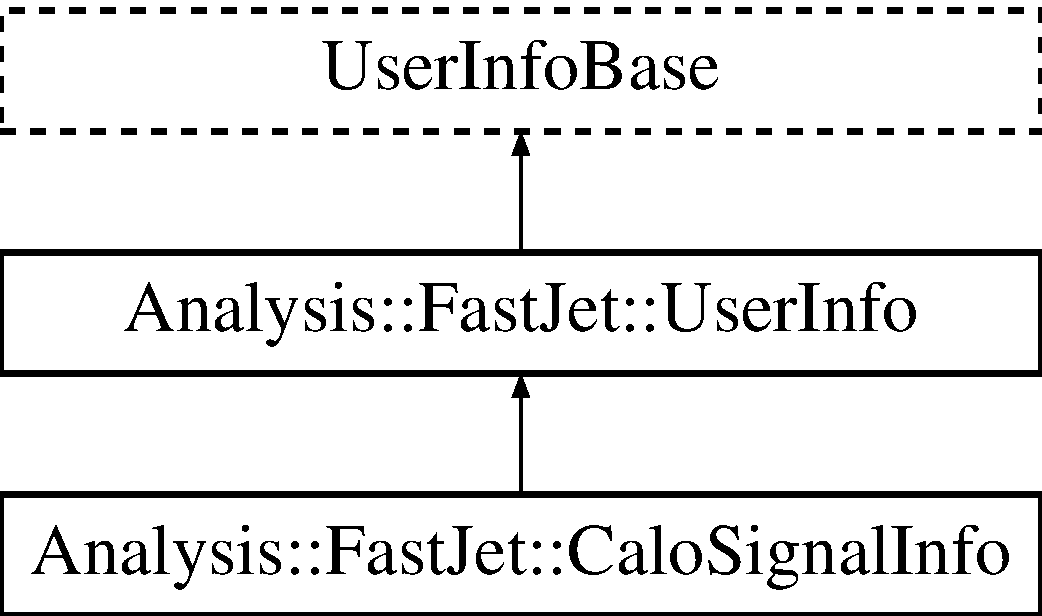
\includegraphics[height=3.000000cm]{classAnalysis_1_1FastJet_1_1CaloSignalInfo}
\end{center}
\end{figure}
\subsection*{Public Types}
\begin{DoxyCompactItemize}
\item 
enum \hyperlink{classAnalysis_1_1FastJet_1_1CaloSignalInfo_ac03e8f6d7fb631eab49a9ab02cda7675}{Type} \{ \\*
\hyperlink{classAnalysis_1_1FastJet_1_1CaloSignalInfo_ac03e8f6d7fb631eab49a9ab02cda7675acf1212505f289985f1e261fbbca13484}{Topo\+Cluster} = 0x01, 
\hyperlink{classAnalysis_1_1FastJet_1_1CaloSignalInfo_ac03e8f6d7fb631eab49a9ab02cda7675a8a62dc4a7b24c36d548a3e382d32a403}{Topo\+Tower} =0x02, 
\hyperlink{classAnalysis_1_1FastJet_1_1CaloSignalInfo_ac03e8f6d7fb631eab49a9ab02cda7675adfd6d8fa14b4f9e9e42564c26c0773ae}{Topo\+Tower\+Norm} = 0x02, 
\hyperlink{classAnalysis_1_1FastJet_1_1CaloSignalInfo_ac03e8f6d7fb631eab49a9ab02cda7675aa6b1555b17060efe7771635af1a87519}{Topo\+Tower\+Coarse} = 0x02, 
\\*
\hyperlink{classAnalysis_1_1FastJet_1_1CaloSignalInfo_ac03e8f6d7fb631eab49a9ab02cda7675ae4a6680d4c780d03251c9065791e2792}{Topo\+Tower\+Fine} = 0x04, 
\hyperlink{classAnalysis_1_1FastJet_1_1CaloSignalInfo_ac03e8f6d7fb631eab49a9ab02cda7675a263dc44fe7b5d0fd7c5d761e23c8ea9a}{Unknown} = 0x00
 \}
\end{DoxyCompactItemize}
\subsection*{Public Member Functions}
\begin{DoxyCompactItemize}
\item 
\hyperlink{classAnalysis_1_1FastJet_1_1CaloSignalInfo_a1c052e698143cf8df61401bf14211c63}{Calo\+Signal\+Info} (int idx, \hyperlink{classAnalysis_1_1FastJet_1_1CaloSignalInfo_ac03e8f6d7fb631eab49a9ab02cda7675}{Type} stype)
\item 
\hyperlink{classAnalysis_1_1FastJet_1_1CaloSignalInfo_a6e6e4b3fddd49811dbe358bdd9925e2c}{Calo\+Signal\+Info} ()
\item 
\hyperlink{classAnalysis_1_1FastJet_1_1CaloSignalInfo_ad95c893fa0a848f5e9d236f6f8a95754}{Calo\+Signal\+Info} (const \hyperlink{classAnalysis_1_1FastJet_1_1CaloSignalInfo}{Calo\+Signal\+Info} \&ci)
\item 
\hyperlink{classAnalysis_1_1FastJet_1_1CaloSignalInfo_a44997a907fd4e790004a96ff9839c7b3}{Calo\+Signal\+Info} (const \hyperlink{classAnalysis_1_1FastJet_1_1CaloSignalInfo}{Calo\+Signal\+Info} $\ast$ci)
\item 
virtual \hyperlink{classAnalysis_1_1FastJet_1_1CaloSignalInfo_af5f8d21c9cc239c7353d74901fa23101}{$\sim$\+Calo\+Signal\+Info} ()
\item 
\hyperlink{classAnalysis_1_1FastJet_1_1CaloSignalInfo_ac03e8f6d7fb631eab49a9ab02cda7675}{Type} \hyperlink{classAnalysis_1_1FastJet_1_1CaloSignalInfo_abac003e16f1fae225bb6d3627a71e8ac}{type} () const 
\item 
\hyperlink{classAnalysis_1_1FastJet_1_1CaloSignalInfo_ac03e8f6d7fb631eab49a9ab02cda7675}{Type} \hyperlink{classAnalysis_1_1FastJet_1_1CaloSignalInfo_a4ce902eef34836cb0736e6c133294a69}{type} (const std\+::string \&\hyperlink{classAnalysis_1_1FastJet_1_1CaloSignalInfo_acc8335b43ac3e8cc2cc040c230b50aa3}{type\+Name}) const 
\item 
const std\+::string \& \hyperlink{classAnalysis_1_1FastJet_1_1CaloSignalInfo_acc8335b43ac3e8cc2cc040c230b50aa3}{type\+Name} () const 
\item 
void \hyperlink{classAnalysis_1_1FastJet_1_1CaloSignalInfo_ac8ec46a412dbacf12caca458a0aec2f0}{set\+Area} (double \hyperlink{classAnalysis_1_1FastJet_1_1CaloSignalInfo_a4998572743794def4adae57cf3865a2c}{area})
\item 
void \hyperlink{classAnalysis_1_1FastJet_1_1CaloSignalInfo_a2003366c8743fc150442bf638d15b688}{set\+P\+TD} (double ptd)
\item 
void \hyperlink{classAnalysis_1_1FastJet_1_1CaloSignalInfo_a5e765abf01922d438c57d917d4ed4c73}{set\+E\+P\+OS} (double epos)
\item 
void \hyperlink{classAnalysis_1_1FastJet_1_1CaloSignalInfo_a187b575d702f519644f2182217967b75}{set\+Time} (double \hyperlink{classAnalysis_1_1FastJet_1_1CaloSignalInfo_a74925b32feb684ee5c4629f126519be7}{time})
\item 
void \hyperlink{classAnalysis_1_1FastJet_1_1CaloSignalInfo_a1690e94963b3c31c00dcfbdc8aba7067}{set\+Type} (\hyperlink{classAnalysis_1_1FastJet_1_1CaloSignalInfo_ac03e8f6d7fb631eab49a9ab02cda7675}{Type} type\+Id)
\item 
void \hyperlink{classAnalysis_1_1FastJet_1_1CaloSignalInfo_a41827f5221f07e060ce86d0fd82ddda5}{set\+Type\+Name} (const std\+::string \&\hyperlink{classAnalysis_1_1FastJet_1_1CaloSignalInfo_acc8335b43ac3e8cc2cc040c230b50aa3}{type\+Name})
\item 
void \hyperlink{classAnalysis_1_1FastJet_1_1CaloSignalInfo_a273f8e95a73022aa25565216a4508852}{set\+OrigE} (double e)
\item 
double \hyperlink{classAnalysis_1_1FastJet_1_1CaloSignalInfo_a6c825d60c49876434ca6d5535c8e24e2}{fixed\+Area} () const 
\item 
double \hyperlink{classAnalysis_1_1FastJet_1_1CaloSignalInfo_a4998572743794def4adae57cf3865a2c}{area} () const 
\item 
double \hyperlink{classAnalysis_1_1FastJet_1_1CaloSignalInfo_ae7a8771287aac7e9f3de29768f21fb0d}{P\+TD} () const 
\item 
double \hyperlink{classAnalysis_1_1FastJet_1_1CaloSignalInfo_ad0af2ed179c09d0adf74331e9a4a6e08}{E\+P\+OS} () const 
\item 
double \hyperlink{classAnalysis_1_1FastJet_1_1CaloSignalInfo_a74925b32feb684ee5c4629f126519be7}{time} () const 
\item 
double \hyperlink{classAnalysis_1_1FastJet_1_1CaloSignalInfo_a04cfca843c49a95befabfa6b1dcdc9b3}{origE} () const 
\end{DoxyCompactItemize}
\begin{Indent}{\bf Set object status}\par
{\em Set status to \char`\"{}empty\char`\"{} (no reference data) }\begin{DoxyCompactItemize}
\item 
virtual void \hyperlink{classAnalysis_1_1FastJet_1_1UserInfo_ab87ca9e42c15c24c8f54bad4b9674d0c}{set\+Empty} ()
\begin{DoxyCompactList}\small\item\em Set status to \char`\"{}faulty\char`\"{} (broken/invalid) \end{DoxyCompactList}\item 
virtual void \hyperlink{classAnalysis_1_1FastJet_1_1UserInfo_a0c5efdcfb658e75538dd5ec29c27afe0}{set\+Faulty} ()
\begin{DoxyCompactList}\small\item\em Set status to \char`\"{}faulty\char`\"{} (broken/invalid) \end{DoxyCompactList}\item 
virtual void \hyperlink{classAnalysis_1_1FastJet_1_1UserInfo_ab22ff88713e1ad12bd2311cc4f1c998c}{set\+Ghost} ()
\begin{DoxyCompactList}\small\item\em Set status to \char`\"{}ghosted\char`\"{}. \end{DoxyCompactList}\end{DoxyCompactItemize}
\end{Indent}
\begin{Indent}{\bf Access object status and data}\par
{\em Retrieve reference index (or status indicator)

\begin{DoxyReturn}{Returns}
Reference index if $>$= 0 (may still be invalid -\/ no checking); if $<$0 returns status. 
\end{DoxyReturn}
}\begin{DoxyCompactItemize}
\item 
virtual int \hyperlink{classAnalysis_1_1FastJet_1_1UserInfo_a687e6a814e58e5737108ef24aef047df}{index} () const 
\begin{DoxyCompactList}\small\item\em Check if empty. \end{DoxyCompactList}\item 
virtual bool \hyperlink{classAnalysis_1_1FastJet_1_1UserInfo_a4b987d1bba6c854cf9310596abbd3572}{is\+Empty} () const 
\begin{DoxyCompactList}\small\item\em Check if empty. \end{DoxyCompactList}\item 
virtual bool \hyperlink{classAnalysis_1_1FastJet_1_1UserInfo_a74601c143cb58b3bb62e0842b416beed}{is\+Faulty} () const 
\begin{DoxyCompactList}\small\item\em Check if faulty/broken/invalid. \end{DoxyCompactList}\item 
virtual bool \hyperlink{classAnalysis_1_1FastJet_1_1UserInfo_ad7b1ceba9d2ab04e7e7000577fe95198}{is\+Usable} () const 
\begin{DoxyCompactList}\small\item\em Check if usable. \end{DoxyCompactList}\item 
virtual bool \hyperlink{classAnalysis_1_1FastJet_1_1UserInfo_a92d2abe359ed4b794c546a23a9e1ccbe}{is\+Ghost} () const 
\begin{DoxyCompactList}\small\item\em Check if ghost. \end{DoxyCompactList}\end{DoxyCompactItemize}
\end{Indent}
\subsection*{Static Public Member Functions}
\begin{DoxyCompactItemize}
\item 
static double \hyperlink{classAnalysis_1_1FastJet_1_1CaloSignalInfo_aa4008fb819a90eba42de259914b9f799}{def\+Time} ()
\item 
static bool \hyperlink{classAnalysis_1_1FastJet_1_1CaloSignalInfo_ad3987a22c21aafdb3f074dfe6c15ddd4}{is\+Calo\+Signal} (const fastjet\+::\+Pseudo\+Jet \&pj)
\item 
static bool \hyperlink{classAnalysis_1_1FastJet_1_1CaloSignalInfo_a1d00cdcaf5f0c17d9d6aa07f1ec3e486}{has\+Calo\+Area} (const fastjet\+::\+Pseudo\+Jet \&pj)
\item 
static double \hyperlink{classAnalysis_1_1FastJet_1_1CaloSignalInfo_a5585d0b0e21cf7261fbfdd37d88de689}{calo\+Area} (const fastjet\+::\+Pseudo\+Jet \&pj)
\item 
static double \hyperlink{classAnalysis_1_1FastJet_1_1CaloSignalInfo_ab1772259e0578e51056a8e1cc8cdd342}{calo\+Fixed\+Area} (const fastjet\+::\+Pseudo\+Jet \&pj)
\item 
static double \hyperlink{classAnalysis_1_1FastJet_1_1CaloSignalInfo_a3cc740a3b70b82def83ffb9a6ff43cd3}{calo\+P\+TD} (const fastjet\+::\+Pseudo\+Jet \&pj)
\item 
static double \hyperlink{classAnalysis_1_1FastJet_1_1CaloSignalInfo_ac68b4786735b76e511b2f9b801025833}{calo\+E\+P\+OS} (const fastjet\+::\+Pseudo\+Jet \&pj)
\item 
static const std\+::string \& \hyperlink{classAnalysis_1_1FastJet_1_1CaloSignalInfo_a4bcba28ea7871f884c727df5f4d2520b}{signal\+Name} (const fastjet\+::\+Pseudo\+Jet \&pj)
\item 
static \hyperlink{classAnalysis_1_1FastJet_1_1CaloSignalInfo_ac03e8f6d7fb631eab49a9ab02cda7675}{Type} \hyperlink{classAnalysis_1_1FastJet_1_1CaloSignalInfo_a761a65bf1c957b4d7f0d37cf6f85d351}{signal\+Type} (const fastjet\+::\+Pseudo\+Jet \&pj)
\item 
static double \hyperlink{classAnalysis_1_1FastJet_1_1CaloSignalInfo_a815a75eb24f274d882f700e35aaf34b0}{calo\+Time} (const fastjet\+::\+Pseudo\+Jet \&pj)
\item 
static double \hyperlink{classAnalysis_1_1FastJet_1_1CaloSignalInfo_afb7471b4f7adcd5c4a0fe86f8c7d486b}{origE} (const fastjet\+::\+Pseudo\+Jet \&pj)
\item 
static bool \hyperlink{classAnalysis_1_1FastJet_1_1UserInfo_a79ba59c5af9a4bc2e641ab2e54e8d50b}{is\+Empty} (const fastjet\+::\+Pseudo\+Jet \&pj)
\item 
static bool \hyperlink{classAnalysis_1_1FastJet_1_1UserInfo_a18b23aae344587ff280a046e70af1d29}{is\+Usable} (const fastjet\+::\+Pseudo\+Jet \&pj)
\item 
static bool \hyperlink{classAnalysis_1_1FastJet_1_1UserInfo_a4682fdc7e258328293b05951f55cc7a1}{is\+Ghost} (const fastjet\+::\+Pseudo\+Jet \&pj)
\item 
static bool \hyperlink{classAnalysis_1_1FastJet_1_1UserInfo_a681f1076b15320ea55e7104b4fe01c3a}{has\+User\+Info} (const fastjet\+::\+Pseudo\+Jet \&pj)
\item 
static int \hyperlink{classAnalysis_1_1FastJet_1_1UserInfo_a767f93f891d045f209198cdf72fddf36}{user\+Index} (const fastjet\+::\+Pseudo\+Jet \&pj)
\end{DoxyCompactItemize}
\subsection*{Static Protected Member Functions}
\begin{DoxyCompactItemize}
\item 
static bool \hyperlink{classAnalysis_1_1FastJet_1_1CaloSignalInfo_a60da06d7be16ac2b2456058812c02dd2}{\+\_\+fill\+Maps} ()
\item 
static \hyperlink{classAnalysis_1_1FastJet_1_1CaloSignalInfo_ac03e8f6d7fb631eab49a9ab02cda7675}{Type} \hyperlink{classAnalysis_1_1FastJet_1_1CaloSignalInfo_a5523d02e32bfeac621414ac3708da634}{\+\_\+get\+Type} (const std\+::string \&name)
\item 
static const std\+::string \& \hyperlink{classAnalysis_1_1FastJet_1_1CaloSignalInfo_ae8d06605ae61b010fba0605ccd626681}{\+\_\+get\+Name} (\hyperlink{classAnalysis_1_1FastJet_1_1CaloSignalInfo_ac03e8f6d7fb631eab49a9ab02cda7675}{Type} stype)
\item 
static double \hyperlink{classAnalysis_1_1FastJet_1_1CaloSignalInfo_a100c863de34ba4181d425a4c4609da83}{\+\_\+get\+Fixed\+Area} (\hyperlink{classAnalysis_1_1FastJet_1_1CaloSignalInfo_ac03e8f6d7fb631eab49a9ab02cda7675}{Type} stype)
\end{DoxyCompactItemize}
\subsection*{Protected Attributes}
\begin{DoxyCompactItemize}
\item 
\hyperlink{classAnalysis_1_1FastJet_1_1CaloSignalInfo_ac03e8f6d7fb631eab49a9ab02cda7675}{Type} \hyperlink{classAnalysis_1_1FastJet_1_1CaloSignalInfo_ab46f3aed35f69718e0faa3b4aa4580a7}{\+\_\+type\+Id}
\item 
std\+::string \hyperlink{classAnalysis_1_1FastJet_1_1CaloSignalInfo_ad359585157bcda1da4b08560ce2d4977}{\+\_\+type\+Name}
\item 
double \hyperlink{classAnalysis_1_1FastJet_1_1CaloSignalInfo_aa6d9e317ef5ec7c3e75770e068552190}{\+\_\+area}
\item 
double \hyperlink{classAnalysis_1_1FastJet_1_1CaloSignalInfo_a4824760bad2a7b7683145a95e667a436}{\+\_\+\+P\+TD}
\item 
double \hyperlink{classAnalysis_1_1FastJet_1_1CaloSignalInfo_a332e388462beecce5426c3c3dfd43240}{\+\_\+\+E\+P\+OS}
\item 
double \hyperlink{classAnalysis_1_1FastJet_1_1CaloSignalInfo_ae6fd205bf7cf2490b9fb0f1878e0ae37}{\+\_\+time}
\item 
double \hyperlink{classAnalysis_1_1FastJet_1_1CaloSignalInfo_a55ae2c4227e431ea9f322461173628a6}{\+\_\+origE}
\item 
int \hyperlink{classAnalysis_1_1FastJet_1_1UserInfo_ad9aa33e317aea2b675493b664cc718a3}{\+\_\+idx}
\begin{DoxyCompactList}\small\item\em Index to underlying structure holding data. \end{DoxyCompactList}\end{DoxyCompactItemize}
\subsection*{Static Protected Attributes}
\begin{DoxyCompactItemize}
\item 
static std\+::map$<$ \hyperlink{classAnalysis_1_1FastJet_1_1CaloSignalInfo_ac03e8f6d7fb631eab49a9ab02cda7675}{Type}, std\+::string $>$ \hyperlink{classAnalysis_1_1FastJet_1_1CaloSignalInfo_a02077135796cf03c3d55144e7201c2db}{\+\_\+map\+Type\+Name} = std\+::map$<$\hyperlink{classAnalysis_1_1FastJet_1_1CaloSignalInfo_ac03e8f6d7fb631eab49a9ab02cda7675}{Analysis\+::\+Fast\+Jet\+::\+Calo\+Signal\+Info\+::\+Type},std\+::string$>$()
\item 
static std\+::map$<$ std\+::string, \hyperlink{classAnalysis_1_1FastJet_1_1CaloSignalInfo_ac03e8f6d7fb631eab49a9ab02cda7675}{Type} $>$ \hyperlink{classAnalysis_1_1FastJet_1_1CaloSignalInfo_abf6ff7b4cc2f83468d4c8e4ce19e9845}{\+\_\+map\+Name\+Type} = std\+::map$<$std\+::string,\hyperlink{classAnalysis_1_1FastJet_1_1CaloSignalInfo_ac03e8f6d7fb631eab49a9ab02cda7675}{Analysis\+::\+Fast\+Jet\+::\+Calo\+Signal\+Info\+::\+Type}$>$()
\item 
static std\+::map$<$ \hyperlink{classAnalysis_1_1FastJet_1_1CaloSignalInfo_ac03e8f6d7fb631eab49a9ab02cda7675}{Type}, double $>$ \hyperlink{classAnalysis_1_1FastJet_1_1CaloSignalInfo_a239a18104bf9715d803b912b668fce21}{\+\_\+map\+Fixed\+Area} = std\+::map$<$\hyperlink{classAnalysis_1_1FastJet_1_1CaloSignalInfo_ac03e8f6d7fb631eab49a9ab02cda7675}{Analysis\+::\+Fast\+Jet\+::\+Calo\+Signal\+Info\+::\+Type},double$>$()
\item 
static double \hyperlink{classAnalysis_1_1FastJet_1_1CaloSignalInfo_acd4a5a250d92298dd91d4081be322f72}{\+\_\+def\+Time} = -\/999.
\end{DoxyCompactItemize}


\subsection{Detailed Description}


Definition at line 370 of file Analysis\+Data.\+h.



\subsection{Member Enumeration Documentation}
\index{Analysis\+::\+Fast\+Jet\+::\+Calo\+Signal\+Info@{Analysis\+::\+Fast\+Jet\+::\+Calo\+Signal\+Info}!Type@{Type}}
\index{Type@{Type}!Analysis\+::\+Fast\+Jet\+::\+Calo\+Signal\+Info@{Analysis\+::\+Fast\+Jet\+::\+Calo\+Signal\+Info}}
\subsubsection[{\texorpdfstring{Type}{Type}}]{\setlength{\rightskip}{0pt plus 5cm}enum {\bf Analysis\+::\+Fast\+Jet\+::\+Calo\+Signal\+Info\+::\+Type}}\hypertarget{classAnalysis_1_1FastJet_1_1CaloSignalInfo_ac03e8f6d7fb631eab49a9ab02cda7675}{}\label{classAnalysis_1_1FastJet_1_1CaloSignalInfo_ac03e8f6d7fb631eab49a9ab02cda7675}
\begin{Desc}
\item[Enumerator]\par
\begin{description}
\index{Topo\+Cluster@{Topo\+Cluster}!Analysis\+::\+Fast\+Jet\+::\+Calo\+Signal\+Info@{Analysis\+::\+Fast\+Jet\+::\+Calo\+Signal\+Info}}\index{Analysis\+::\+Fast\+Jet\+::\+Calo\+Signal\+Info@{Analysis\+::\+Fast\+Jet\+::\+Calo\+Signal\+Info}!Topo\+Cluster@{Topo\+Cluster}}\item[{\em 
Topo\+Cluster\hypertarget{classAnalysis_1_1FastJet_1_1CaloSignalInfo_ac03e8f6d7fb631eab49a9ab02cda7675acf1212505f289985f1e261fbbca13484}{}\label{classAnalysis_1_1FastJet_1_1CaloSignalInfo_ac03e8f6d7fb631eab49a9ab02cda7675acf1212505f289985f1e261fbbca13484}
}]\index{Topo\+Tower@{Topo\+Tower}!Analysis\+::\+Fast\+Jet\+::\+Calo\+Signal\+Info@{Analysis\+::\+Fast\+Jet\+::\+Calo\+Signal\+Info}}\index{Analysis\+::\+Fast\+Jet\+::\+Calo\+Signal\+Info@{Analysis\+::\+Fast\+Jet\+::\+Calo\+Signal\+Info}!Topo\+Tower@{Topo\+Tower}}\item[{\em 
Topo\+Tower\hypertarget{classAnalysis_1_1FastJet_1_1CaloSignalInfo_ac03e8f6d7fb631eab49a9ab02cda7675a8a62dc4a7b24c36d548a3e382d32a403}{}\label{classAnalysis_1_1FastJet_1_1CaloSignalInfo_ac03e8f6d7fb631eab49a9ab02cda7675a8a62dc4a7b24c36d548a3e382d32a403}
}]\index{Topo\+Tower\+Norm@{Topo\+Tower\+Norm}!Analysis\+::\+Fast\+Jet\+::\+Calo\+Signal\+Info@{Analysis\+::\+Fast\+Jet\+::\+Calo\+Signal\+Info}}\index{Analysis\+::\+Fast\+Jet\+::\+Calo\+Signal\+Info@{Analysis\+::\+Fast\+Jet\+::\+Calo\+Signal\+Info}!Topo\+Tower\+Norm@{Topo\+Tower\+Norm}}\item[{\em 
Topo\+Tower\+Norm\hypertarget{classAnalysis_1_1FastJet_1_1CaloSignalInfo_ac03e8f6d7fb631eab49a9ab02cda7675adfd6d8fa14b4f9e9e42564c26c0773ae}{}\label{classAnalysis_1_1FastJet_1_1CaloSignalInfo_ac03e8f6d7fb631eab49a9ab02cda7675adfd6d8fa14b4f9e9e42564c26c0773ae}
}]\index{Topo\+Tower\+Coarse@{Topo\+Tower\+Coarse}!Analysis\+::\+Fast\+Jet\+::\+Calo\+Signal\+Info@{Analysis\+::\+Fast\+Jet\+::\+Calo\+Signal\+Info}}\index{Analysis\+::\+Fast\+Jet\+::\+Calo\+Signal\+Info@{Analysis\+::\+Fast\+Jet\+::\+Calo\+Signal\+Info}!Topo\+Tower\+Coarse@{Topo\+Tower\+Coarse}}\item[{\em 
Topo\+Tower\+Coarse\hypertarget{classAnalysis_1_1FastJet_1_1CaloSignalInfo_ac03e8f6d7fb631eab49a9ab02cda7675aa6b1555b17060efe7771635af1a87519}{}\label{classAnalysis_1_1FastJet_1_1CaloSignalInfo_ac03e8f6d7fb631eab49a9ab02cda7675aa6b1555b17060efe7771635af1a87519}
}]\index{Topo\+Tower\+Fine@{Topo\+Tower\+Fine}!Analysis\+::\+Fast\+Jet\+::\+Calo\+Signal\+Info@{Analysis\+::\+Fast\+Jet\+::\+Calo\+Signal\+Info}}\index{Analysis\+::\+Fast\+Jet\+::\+Calo\+Signal\+Info@{Analysis\+::\+Fast\+Jet\+::\+Calo\+Signal\+Info}!Topo\+Tower\+Fine@{Topo\+Tower\+Fine}}\item[{\em 
Topo\+Tower\+Fine\hypertarget{classAnalysis_1_1FastJet_1_1CaloSignalInfo_ac03e8f6d7fb631eab49a9ab02cda7675ae4a6680d4c780d03251c9065791e2792}{}\label{classAnalysis_1_1FastJet_1_1CaloSignalInfo_ac03e8f6d7fb631eab49a9ab02cda7675ae4a6680d4c780d03251c9065791e2792}
}]\index{Unknown@{Unknown}!Analysis\+::\+Fast\+Jet\+::\+Calo\+Signal\+Info@{Analysis\+::\+Fast\+Jet\+::\+Calo\+Signal\+Info}}\index{Analysis\+::\+Fast\+Jet\+::\+Calo\+Signal\+Info@{Analysis\+::\+Fast\+Jet\+::\+Calo\+Signal\+Info}!Unknown@{Unknown}}\item[{\em 
Unknown\hypertarget{classAnalysis_1_1FastJet_1_1CaloSignalInfo_ac03e8f6d7fb631eab49a9ab02cda7675a263dc44fe7b5d0fd7c5d761e23c8ea9a}{}\label{classAnalysis_1_1FastJet_1_1CaloSignalInfo_ac03e8f6d7fb631eab49a9ab02cda7675a263dc44fe7b5d0fd7c5d761e23c8ea9a}
}]\end{description}
\end{Desc}


Definition at line 373 of file Analysis\+Data.\+h.



\subsection{Constructor \& Destructor Documentation}
\index{Analysis\+::\+Fast\+Jet\+::\+Calo\+Signal\+Info@{Analysis\+::\+Fast\+Jet\+::\+Calo\+Signal\+Info}!Calo\+Signal\+Info@{Calo\+Signal\+Info}}
\index{Calo\+Signal\+Info@{Calo\+Signal\+Info}!Analysis\+::\+Fast\+Jet\+::\+Calo\+Signal\+Info@{Analysis\+::\+Fast\+Jet\+::\+Calo\+Signal\+Info}}
\subsubsection[{\texorpdfstring{Calo\+Signal\+Info(int idx, Type stype)}{CaloSignalInfo(int idx, Type stype)}}]{\setlength{\rightskip}{0pt plus 5cm}Analysis\+::\+Fast\+Jet\+::\+Calo\+Signal\+Info\+::\+Calo\+Signal\+Info (
\begin{DoxyParamCaption}
\item[{int}]{idx, }
\item[{{\bf Type}}]{stype}
\end{DoxyParamCaption}
)\hspace{0.3cm}{\ttfamily [inline]}}\hypertarget{classAnalysis_1_1FastJet_1_1CaloSignalInfo_a1c052e698143cf8df61401bf14211c63}{}\label{classAnalysis_1_1FastJet_1_1CaloSignalInfo_a1c052e698143cf8df61401bf14211c63}


Definition at line 412 of file Analysis\+Data.\+h.

\index{Analysis\+::\+Fast\+Jet\+::\+Calo\+Signal\+Info@{Analysis\+::\+Fast\+Jet\+::\+Calo\+Signal\+Info}!Calo\+Signal\+Info@{Calo\+Signal\+Info}}
\index{Calo\+Signal\+Info@{Calo\+Signal\+Info}!Analysis\+::\+Fast\+Jet\+::\+Calo\+Signal\+Info@{Analysis\+::\+Fast\+Jet\+::\+Calo\+Signal\+Info}}
\subsubsection[{\texorpdfstring{Calo\+Signal\+Info()}{CaloSignalInfo()}}]{\setlength{\rightskip}{0pt plus 5cm}Analysis\+::\+Fast\+Jet\+::\+Calo\+Signal\+Info\+::\+Calo\+Signal\+Info (
\begin{DoxyParamCaption}
{}
\end{DoxyParamCaption}
)\hspace{0.3cm}{\ttfamily [inline]}}\hypertarget{classAnalysis_1_1FastJet_1_1CaloSignalInfo_a6e6e4b3fddd49811dbe358bdd9925e2c}{}\label{classAnalysis_1_1FastJet_1_1CaloSignalInfo_a6e6e4b3fddd49811dbe358bdd9925e2c}


Definition at line 422 of file Analysis\+Data.\+h.

\index{Analysis\+::\+Fast\+Jet\+::\+Calo\+Signal\+Info@{Analysis\+::\+Fast\+Jet\+::\+Calo\+Signal\+Info}!Calo\+Signal\+Info@{Calo\+Signal\+Info}}
\index{Calo\+Signal\+Info@{Calo\+Signal\+Info}!Analysis\+::\+Fast\+Jet\+::\+Calo\+Signal\+Info@{Analysis\+::\+Fast\+Jet\+::\+Calo\+Signal\+Info}}
\subsubsection[{\texorpdfstring{Calo\+Signal\+Info(const Calo\+Signal\+Info \&ci)}{CaloSignalInfo(const CaloSignalInfo &ci)}}]{\setlength{\rightskip}{0pt plus 5cm}Analysis\+::\+Fast\+Jet\+::\+Calo\+Signal\+Info\+::\+Calo\+Signal\+Info (
\begin{DoxyParamCaption}
\item[{const {\bf Calo\+Signal\+Info} \&}]{ci}
\end{DoxyParamCaption}
)\hspace{0.3cm}{\ttfamily [inline]}}\hypertarget{classAnalysis_1_1FastJet_1_1CaloSignalInfo_ad95c893fa0a848f5e9d236f6f8a95754}{}\label{classAnalysis_1_1FastJet_1_1CaloSignalInfo_ad95c893fa0a848f5e9d236f6f8a95754}


Definition at line 432 of file Analysis\+Data.\+h.

\index{Analysis\+::\+Fast\+Jet\+::\+Calo\+Signal\+Info@{Analysis\+::\+Fast\+Jet\+::\+Calo\+Signal\+Info}!Calo\+Signal\+Info@{Calo\+Signal\+Info}}
\index{Calo\+Signal\+Info@{Calo\+Signal\+Info}!Analysis\+::\+Fast\+Jet\+::\+Calo\+Signal\+Info@{Analysis\+::\+Fast\+Jet\+::\+Calo\+Signal\+Info}}
\subsubsection[{\texorpdfstring{Calo\+Signal\+Info(const Calo\+Signal\+Info $\ast$ci)}{CaloSignalInfo(const CaloSignalInfo *ci)}}]{\setlength{\rightskip}{0pt plus 5cm}Analysis\+::\+Fast\+Jet\+::\+Calo\+Signal\+Info\+::\+Calo\+Signal\+Info (
\begin{DoxyParamCaption}
\item[{const {\bf Calo\+Signal\+Info} $\ast$}]{ci}
\end{DoxyParamCaption}
)\hspace{0.3cm}{\ttfamily [inline]}}\hypertarget{classAnalysis_1_1FastJet_1_1CaloSignalInfo_a44997a907fd4e790004a96ff9839c7b3}{}\label{classAnalysis_1_1FastJet_1_1CaloSignalInfo_a44997a907fd4e790004a96ff9839c7b3}


Definition at line 442 of file Analysis\+Data.\+h.

\index{Analysis\+::\+Fast\+Jet\+::\+Calo\+Signal\+Info@{Analysis\+::\+Fast\+Jet\+::\+Calo\+Signal\+Info}!````~Calo\+Signal\+Info@{$\sim$\+Calo\+Signal\+Info}}
\index{````~Calo\+Signal\+Info@{$\sim$\+Calo\+Signal\+Info}!Analysis\+::\+Fast\+Jet\+::\+Calo\+Signal\+Info@{Analysis\+::\+Fast\+Jet\+::\+Calo\+Signal\+Info}}
\subsubsection[{\texorpdfstring{$\sim$\+Calo\+Signal\+Info()}{~CaloSignalInfo()}}]{\setlength{\rightskip}{0pt plus 5cm}virtual Analysis\+::\+Fast\+Jet\+::\+Calo\+Signal\+Info\+::$\sim$\+Calo\+Signal\+Info (
\begin{DoxyParamCaption}
{}
\end{DoxyParamCaption}
)\hspace{0.3cm}{\ttfamily [inline]}, {\ttfamily [virtual]}}\hypertarget{classAnalysis_1_1FastJet_1_1CaloSignalInfo_af5f8d21c9cc239c7353d74901fa23101}{}\label{classAnalysis_1_1FastJet_1_1CaloSignalInfo_af5f8d21c9cc239c7353d74901fa23101}


Definition at line 443 of file Analysis\+Data.\+h.



\subsection{Member Function Documentation}
\index{Analysis\+::\+Fast\+Jet\+::\+Calo\+Signal\+Info@{Analysis\+::\+Fast\+Jet\+::\+Calo\+Signal\+Info}!\+\_\+fill\+Maps@{\+\_\+fill\+Maps}}
\index{\+\_\+fill\+Maps@{\+\_\+fill\+Maps}!Analysis\+::\+Fast\+Jet\+::\+Calo\+Signal\+Info@{Analysis\+::\+Fast\+Jet\+::\+Calo\+Signal\+Info}}
\subsubsection[{\texorpdfstring{\+\_\+fill\+Maps()}{_fillMaps()}}]{\setlength{\rightskip}{0pt plus 5cm}static bool Analysis\+::\+Fast\+Jet\+::\+Calo\+Signal\+Info\+::\+\_\+fill\+Maps (
\begin{DoxyParamCaption}
{}
\end{DoxyParamCaption}
)\hspace{0.3cm}{\ttfamily [inline]}, {\ttfamily [static]}, {\ttfamily [protected]}}\hypertarget{classAnalysis_1_1FastJet_1_1CaloSignalInfo_a60da06d7be16ac2b2456058812c02dd2}{}\label{classAnalysis_1_1FastJet_1_1CaloSignalInfo_a60da06d7be16ac2b2456058812c02dd2}


Definition at line 379 of file Analysis\+Data.\+h.

\index{Analysis\+::\+Fast\+Jet\+::\+Calo\+Signal\+Info@{Analysis\+::\+Fast\+Jet\+::\+Calo\+Signal\+Info}!\+\_\+get\+Fixed\+Area@{\+\_\+get\+Fixed\+Area}}
\index{\+\_\+get\+Fixed\+Area@{\+\_\+get\+Fixed\+Area}!Analysis\+::\+Fast\+Jet\+::\+Calo\+Signal\+Info@{Analysis\+::\+Fast\+Jet\+::\+Calo\+Signal\+Info}}
\subsubsection[{\texorpdfstring{\+\_\+get\+Fixed\+Area(\+Type stype)}{_getFixedArea(Type stype)}}]{\setlength{\rightskip}{0pt plus 5cm}static double Analysis\+::\+Fast\+Jet\+::\+Calo\+Signal\+Info\+::\+\_\+get\+Fixed\+Area (
\begin{DoxyParamCaption}
\item[{{\bf Type}}]{stype}
\end{DoxyParamCaption}
)\hspace{0.3cm}{\ttfamily [inline]}, {\ttfamily [static]}, {\ttfamily [protected]}}\hypertarget{classAnalysis_1_1FastJet_1_1CaloSignalInfo_a100c863de34ba4181d425a4c4609da83}{}\label{classAnalysis_1_1FastJet_1_1CaloSignalInfo_a100c863de34ba4181d425a4c4609da83}


Definition at line 396 of file Analysis\+Data.\+h.

\index{Analysis\+::\+Fast\+Jet\+::\+Calo\+Signal\+Info@{Analysis\+::\+Fast\+Jet\+::\+Calo\+Signal\+Info}!\+\_\+get\+Name@{\+\_\+get\+Name}}
\index{\+\_\+get\+Name@{\+\_\+get\+Name}!Analysis\+::\+Fast\+Jet\+::\+Calo\+Signal\+Info@{Analysis\+::\+Fast\+Jet\+::\+Calo\+Signal\+Info}}
\subsubsection[{\texorpdfstring{\+\_\+get\+Name(\+Type stype)}{_getName(Type stype)}}]{\setlength{\rightskip}{0pt plus 5cm}static const std\+::string\& Analysis\+::\+Fast\+Jet\+::\+Calo\+Signal\+Info\+::\+\_\+get\+Name (
\begin{DoxyParamCaption}
\item[{{\bf Type}}]{stype}
\end{DoxyParamCaption}
)\hspace{0.3cm}{\ttfamily [inline]}, {\ttfamily [static]}, {\ttfamily [protected]}}\hypertarget{classAnalysis_1_1FastJet_1_1CaloSignalInfo_ae8d06605ae61b010fba0605ccd626681}{}\label{classAnalysis_1_1FastJet_1_1CaloSignalInfo_ae8d06605ae61b010fba0605ccd626681}


Definition at line 391 of file Analysis\+Data.\+h.

\index{Analysis\+::\+Fast\+Jet\+::\+Calo\+Signal\+Info@{Analysis\+::\+Fast\+Jet\+::\+Calo\+Signal\+Info}!\+\_\+get\+Type@{\+\_\+get\+Type}}
\index{\+\_\+get\+Type@{\+\_\+get\+Type}!Analysis\+::\+Fast\+Jet\+::\+Calo\+Signal\+Info@{Analysis\+::\+Fast\+Jet\+::\+Calo\+Signal\+Info}}
\subsubsection[{\texorpdfstring{\+\_\+get\+Type(const std\+::string \&name)}{_getType(const std::string &name)}}]{\setlength{\rightskip}{0pt plus 5cm}static {\bf Type} Analysis\+::\+Fast\+Jet\+::\+Calo\+Signal\+Info\+::\+\_\+get\+Type (
\begin{DoxyParamCaption}
\item[{const std\+::string \&}]{name}
\end{DoxyParamCaption}
)\hspace{0.3cm}{\ttfamily [inline]}, {\ttfamily [static]}, {\ttfamily [protected]}}\hypertarget{classAnalysis_1_1FastJet_1_1CaloSignalInfo_a5523d02e32bfeac621414ac3708da634}{}\label{classAnalysis_1_1FastJet_1_1CaloSignalInfo_a5523d02e32bfeac621414ac3708da634}


Definition at line 386 of file Analysis\+Data.\+h.

\index{Analysis\+::\+Fast\+Jet\+::\+Calo\+Signal\+Info@{Analysis\+::\+Fast\+Jet\+::\+Calo\+Signal\+Info}!area@{area}}
\index{area@{area}!Analysis\+::\+Fast\+Jet\+::\+Calo\+Signal\+Info@{Analysis\+::\+Fast\+Jet\+::\+Calo\+Signal\+Info}}
\subsubsection[{\texorpdfstring{area() const }{area() const }}]{\setlength{\rightskip}{0pt plus 5cm}double Analysis\+::\+Fast\+Jet\+::\+Calo\+Signal\+Info\+::area (
\begin{DoxyParamCaption}
{}
\end{DoxyParamCaption}
) const\hspace{0.3cm}{\ttfamily [inline]}}\hypertarget{classAnalysis_1_1FastJet_1_1CaloSignalInfo_a4998572743794def4adae57cf3865a2c}{}\label{classAnalysis_1_1FastJet_1_1CaloSignalInfo_a4998572743794def4adae57cf3865a2c}


Definition at line 458 of file Analysis\+Data.\+h.

\index{Analysis\+::\+Fast\+Jet\+::\+Calo\+Signal\+Info@{Analysis\+::\+Fast\+Jet\+::\+Calo\+Signal\+Info}!calo\+Area@{calo\+Area}}
\index{calo\+Area@{calo\+Area}!Analysis\+::\+Fast\+Jet\+::\+Calo\+Signal\+Info@{Analysis\+::\+Fast\+Jet\+::\+Calo\+Signal\+Info}}
\subsubsection[{\texorpdfstring{calo\+Area(const fastjet\+::\+Pseudo\+Jet \&pj)}{caloArea(const fastjet::PseudoJet &pj)}}]{\setlength{\rightskip}{0pt plus 5cm}static double Analysis\+::\+Fast\+Jet\+::\+Calo\+Signal\+Info\+::calo\+Area (
\begin{DoxyParamCaption}
\item[{const fastjet\+::\+Pseudo\+Jet \&}]{pj}
\end{DoxyParamCaption}
)\hspace{0.3cm}{\ttfamily [inline]}, {\ttfamily [static]}}\hypertarget{classAnalysis_1_1FastJet_1_1CaloSignalInfo_a5585d0b0e21cf7261fbfdd37d88de689}{}\label{classAnalysis_1_1FastJet_1_1CaloSignalInfo_a5585d0b0e21cf7261fbfdd37d88de689}


Definition at line 467 of file Analysis\+Data.\+h.

\index{Analysis\+::\+Fast\+Jet\+::\+Calo\+Signal\+Info@{Analysis\+::\+Fast\+Jet\+::\+Calo\+Signal\+Info}!calo\+E\+P\+OS@{calo\+E\+P\+OS}}
\index{calo\+E\+P\+OS@{calo\+E\+P\+OS}!Analysis\+::\+Fast\+Jet\+::\+Calo\+Signal\+Info@{Analysis\+::\+Fast\+Jet\+::\+Calo\+Signal\+Info}}
\subsubsection[{\texorpdfstring{calo\+E\+P\+O\+S(const fastjet\+::\+Pseudo\+Jet \&pj)}{caloEPOS(const fastjet::PseudoJet &pj)}}]{\setlength{\rightskip}{0pt plus 5cm}static double Analysis\+::\+Fast\+Jet\+::\+Calo\+Signal\+Info\+::calo\+E\+P\+OS (
\begin{DoxyParamCaption}
\item[{const fastjet\+::\+Pseudo\+Jet \&}]{pj}
\end{DoxyParamCaption}
)\hspace{0.3cm}{\ttfamily [inline]}, {\ttfamily [static]}}\hypertarget{classAnalysis_1_1FastJet_1_1CaloSignalInfo_ac68b4786735b76e511b2f9b801025833}{}\label{classAnalysis_1_1FastJet_1_1CaloSignalInfo_ac68b4786735b76e511b2f9b801025833}


Definition at line 470 of file Analysis\+Data.\+h.

\index{Analysis\+::\+Fast\+Jet\+::\+Calo\+Signal\+Info@{Analysis\+::\+Fast\+Jet\+::\+Calo\+Signal\+Info}!calo\+Fixed\+Area@{calo\+Fixed\+Area}}
\index{calo\+Fixed\+Area@{calo\+Fixed\+Area}!Analysis\+::\+Fast\+Jet\+::\+Calo\+Signal\+Info@{Analysis\+::\+Fast\+Jet\+::\+Calo\+Signal\+Info}}
\subsubsection[{\texorpdfstring{calo\+Fixed\+Area(const fastjet\+::\+Pseudo\+Jet \&pj)}{caloFixedArea(const fastjet::PseudoJet &pj)}}]{\setlength{\rightskip}{0pt plus 5cm}static double Analysis\+::\+Fast\+Jet\+::\+Calo\+Signal\+Info\+::calo\+Fixed\+Area (
\begin{DoxyParamCaption}
\item[{const fastjet\+::\+Pseudo\+Jet \&}]{pj}
\end{DoxyParamCaption}
)\hspace{0.3cm}{\ttfamily [inline]}, {\ttfamily [static]}}\hypertarget{classAnalysis_1_1FastJet_1_1CaloSignalInfo_ab1772259e0578e51056a8e1cc8cdd342}{}\label{classAnalysis_1_1FastJet_1_1CaloSignalInfo_ab1772259e0578e51056a8e1cc8cdd342}


Definition at line 468 of file Analysis\+Data.\+h.

\index{Analysis\+::\+Fast\+Jet\+::\+Calo\+Signal\+Info@{Analysis\+::\+Fast\+Jet\+::\+Calo\+Signal\+Info}!calo\+P\+TD@{calo\+P\+TD}}
\index{calo\+P\+TD@{calo\+P\+TD}!Analysis\+::\+Fast\+Jet\+::\+Calo\+Signal\+Info@{Analysis\+::\+Fast\+Jet\+::\+Calo\+Signal\+Info}}
\subsubsection[{\texorpdfstring{calo\+P\+T\+D(const fastjet\+::\+Pseudo\+Jet \&pj)}{caloPTD(const fastjet::PseudoJet &pj)}}]{\setlength{\rightskip}{0pt plus 5cm}static double Analysis\+::\+Fast\+Jet\+::\+Calo\+Signal\+Info\+::calo\+P\+TD (
\begin{DoxyParamCaption}
\item[{const fastjet\+::\+Pseudo\+Jet \&}]{pj}
\end{DoxyParamCaption}
)\hspace{0.3cm}{\ttfamily [inline]}, {\ttfamily [static]}}\hypertarget{classAnalysis_1_1FastJet_1_1CaloSignalInfo_a3cc740a3b70b82def83ffb9a6ff43cd3}{}\label{classAnalysis_1_1FastJet_1_1CaloSignalInfo_a3cc740a3b70b82def83ffb9a6ff43cd3}


Definition at line 469 of file Analysis\+Data.\+h.

\index{Analysis\+::\+Fast\+Jet\+::\+Calo\+Signal\+Info@{Analysis\+::\+Fast\+Jet\+::\+Calo\+Signal\+Info}!calo\+Time@{calo\+Time}}
\index{calo\+Time@{calo\+Time}!Analysis\+::\+Fast\+Jet\+::\+Calo\+Signal\+Info@{Analysis\+::\+Fast\+Jet\+::\+Calo\+Signal\+Info}}
\subsubsection[{\texorpdfstring{calo\+Time(const fastjet\+::\+Pseudo\+Jet \&pj)}{caloTime(const fastjet::PseudoJet &pj)}}]{\setlength{\rightskip}{0pt plus 5cm}static double Analysis\+::\+Fast\+Jet\+::\+Calo\+Signal\+Info\+::calo\+Time (
\begin{DoxyParamCaption}
\item[{const fastjet\+::\+Pseudo\+Jet \&}]{pj}
\end{DoxyParamCaption}
)\hspace{0.3cm}{\ttfamily [inline]}, {\ttfamily [static]}}\hypertarget{classAnalysis_1_1FastJet_1_1CaloSignalInfo_a815a75eb24f274d882f700e35aaf34b0}{}\label{classAnalysis_1_1FastJet_1_1CaloSignalInfo_a815a75eb24f274d882f700e35aaf34b0}


Definition at line 473 of file Analysis\+Data.\+h.

\index{Analysis\+::\+Fast\+Jet\+::\+Calo\+Signal\+Info@{Analysis\+::\+Fast\+Jet\+::\+Calo\+Signal\+Info}!def\+Time@{def\+Time}}
\index{def\+Time@{def\+Time}!Analysis\+::\+Fast\+Jet\+::\+Calo\+Signal\+Info@{Analysis\+::\+Fast\+Jet\+::\+Calo\+Signal\+Info}}
\subsubsection[{\texorpdfstring{def\+Time()}{defTime()}}]{\setlength{\rightskip}{0pt plus 5cm}static double Analysis\+::\+Fast\+Jet\+::\+Calo\+Signal\+Info\+::def\+Time (
\begin{DoxyParamCaption}
{}
\end{DoxyParamCaption}
)\hspace{0.3cm}{\ttfamily [inline]}, {\ttfamily [static]}}\hypertarget{classAnalysis_1_1FastJet_1_1CaloSignalInfo_aa4008fb819a90eba42de259914b9f799}{}\label{classAnalysis_1_1FastJet_1_1CaloSignalInfo_aa4008fb819a90eba42de259914b9f799}


Definition at line 462 of file Analysis\+Data.\+h.

\index{Analysis\+::\+Fast\+Jet\+::\+Calo\+Signal\+Info@{Analysis\+::\+Fast\+Jet\+::\+Calo\+Signal\+Info}!E\+P\+OS@{E\+P\+OS}}
\index{E\+P\+OS@{E\+P\+OS}!Analysis\+::\+Fast\+Jet\+::\+Calo\+Signal\+Info@{Analysis\+::\+Fast\+Jet\+::\+Calo\+Signal\+Info}}
\subsubsection[{\texorpdfstring{E\+P\+O\+S() const }{EPOS() const }}]{\setlength{\rightskip}{0pt plus 5cm}double Analysis\+::\+Fast\+Jet\+::\+Calo\+Signal\+Info\+::\+E\+P\+OS (
\begin{DoxyParamCaption}
{}
\end{DoxyParamCaption}
) const\hspace{0.3cm}{\ttfamily [inline]}}\hypertarget{classAnalysis_1_1FastJet_1_1CaloSignalInfo_ad0af2ed179c09d0adf74331e9a4a6e08}{}\label{classAnalysis_1_1FastJet_1_1CaloSignalInfo_ad0af2ed179c09d0adf74331e9a4a6e08}


Definition at line 460 of file Analysis\+Data.\+h.

\index{Analysis\+::\+Fast\+Jet\+::\+Calo\+Signal\+Info@{Analysis\+::\+Fast\+Jet\+::\+Calo\+Signal\+Info}!fixed\+Area@{fixed\+Area}}
\index{fixed\+Area@{fixed\+Area}!Analysis\+::\+Fast\+Jet\+::\+Calo\+Signal\+Info@{Analysis\+::\+Fast\+Jet\+::\+Calo\+Signal\+Info}}
\subsubsection[{\texorpdfstring{fixed\+Area() const }{fixedArea() const }}]{\setlength{\rightskip}{0pt plus 5cm}double Analysis\+::\+Fast\+Jet\+::\+Calo\+Signal\+Info\+::fixed\+Area (
\begin{DoxyParamCaption}
{}
\end{DoxyParamCaption}
) const\hspace{0.3cm}{\ttfamily [inline]}}\hypertarget{classAnalysis_1_1FastJet_1_1CaloSignalInfo_a6c825d60c49876434ca6d5535c8e24e2}{}\label{classAnalysis_1_1FastJet_1_1CaloSignalInfo_a6c825d60c49876434ca6d5535c8e24e2}


Definition at line 457 of file Analysis\+Data.\+h.

\index{Analysis\+::\+Fast\+Jet\+::\+Calo\+Signal\+Info@{Analysis\+::\+Fast\+Jet\+::\+Calo\+Signal\+Info}!has\+Calo\+Area@{has\+Calo\+Area}}
\index{has\+Calo\+Area@{has\+Calo\+Area}!Analysis\+::\+Fast\+Jet\+::\+Calo\+Signal\+Info@{Analysis\+::\+Fast\+Jet\+::\+Calo\+Signal\+Info}}
\subsubsection[{\texorpdfstring{has\+Calo\+Area(const fastjet\+::\+Pseudo\+Jet \&pj)}{hasCaloArea(const fastjet::PseudoJet &pj)}}]{\setlength{\rightskip}{0pt plus 5cm}static bool Analysis\+::\+Fast\+Jet\+::\+Calo\+Signal\+Info\+::has\+Calo\+Area (
\begin{DoxyParamCaption}
\item[{const fastjet\+::\+Pseudo\+Jet \&}]{pj}
\end{DoxyParamCaption}
)\hspace{0.3cm}{\ttfamily [inline]}, {\ttfamily [static]}}\hypertarget{classAnalysis_1_1FastJet_1_1CaloSignalInfo_a1d00cdcaf5f0c17d9d6aa07f1ec3e486}{}\label{classAnalysis_1_1FastJet_1_1CaloSignalInfo_a1d00cdcaf5f0c17d9d6aa07f1ec3e486}


Definition at line 466 of file Analysis\+Data.\+h.

\index{Analysis\+::\+Fast\+Jet\+::\+Calo\+Signal\+Info@{Analysis\+::\+Fast\+Jet\+::\+Calo\+Signal\+Info}!has\+User\+Info@{has\+User\+Info}}
\index{has\+User\+Info@{has\+User\+Info}!Analysis\+::\+Fast\+Jet\+::\+Calo\+Signal\+Info@{Analysis\+::\+Fast\+Jet\+::\+Calo\+Signal\+Info}}
\subsubsection[{\texorpdfstring{has\+User\+Info(const fastjet\+::\+Pseudo\+Jet \&pj)}{hasUserInfo(const fastjet::PseudoJet &pj)}}]{\setlength{\rightskip}{0pt plus 5cm}static bool Analysis\+::\+Fast\+Jet\+::\+User\+Info\+::has\+User\+Info (
\begin{DoxyParamCaption}
\item[{const fastjet\+::\+Pseudo\+Jet \&}]{pj}
\end{DoxyParamCaption}
)\hspace{0.3cm}{\ttfamily [inline]}, {\ttfamily [static]}, {\ttfamily [inherited]}}\hypertarget{classAnalysis_1_1FastJet_1_1UserInfo_a681f1076b15320ea55e7104b4fe01c3a}{}\label{classAnalysis_1_1FastJet_1_1UserInfo_a681f1076b15320ea55e7104b4fe01c3a}


Definition at line 357 of file Analysis\+Data.\+h.

\index{Analysis\+::\+Fast\+Jet\+::\+Calo\+Signal\+Info@{Analysis\+::\+Fast\+Jet\+::\+Calo\+Signal\+Info}!index@{index}}
\index{index@{index}!Analysis\+::\+Fast\+Jet\+::\+Calo\+Signal\+Info@{Analysis\+::\+Fast\+Jet\+::\+Calo\+Signal\+Info}}
\subsubsection[{\texorpdfstring{index() const }{index() const }}]{\setlength{\rightskip}{0pt plus 5cm}virtual int Analysis\+::\+Fast\+Jet\+::\+User\+Info\+::index (
\begin{DoxyParamCaption}
{}
\end{DoxyParamCaption}
) const\hspace{0.3cm}{\ttfamily [inline]}, {\ttfamily [virtual]}, {\ttfamily [inherited]}}\hypertarget{classAnalysis_1_1FastJet_1_1UserInfo_a687e6a814e58e5737108ef24aef047df}{}\label{classAnalysis_1_1FastJet_1_1UserInfo_a687e6a814e58e5737108ef24aef047df}


Check if empty. 

\begin{DoxyReturn}{Returns}
{\ttfamily true} if empty. 
\end{DoxyReturn}


Definition at line 338 of file Analysis\+Data.\+h.

\index{Analysis\+::\+Fast\+Jet\+::\+Calo\+Signal\+Info@{Analysis\+::\+Fast\+Jet\+::\+Calo\+Signal\+Info}!is\+Calo\+Signal@{is\+Calo\+Signal}}
\index{is\+Calo\+Signal@{is\+Calo\+Signal}!Analysis\+::\+Fast\+Jet\+::\+Calo\+Signal\+Info@{Analysis\+::\+Fast\+Jet\+::\+Calo\+Signal\+Info}}
\subsubsection[{\texorpdfstring{is\+Calo\+Signal(const fastjet\+::\+Pseudo\+Jet \&pj)}{isCaloSignal(const fastjet::PseudoJet &pj)}}]{\setlength{\rightskip}{0pt plus 5cm}static bool Analysis\+::\+Fast\+Jet\+::\+Calo\+Signal\+Info\+::is\+Calo\+Signal (
\begin{DoxyParamCaption}
\item[{const fastjet\+::\+Pseudo\+Jet \&}]{pj}
\end{DoxyParamCaption}
)\hspace{0.3cm}{\ttfamily [inline]}, {\ttfamily [static]}}\hypertarget{classAnalysis_1_1FastJet_1_1CaloSignalInfo_ad3987a22c21aafdb3f074dfe6c15ddd4}{}\label{classAnalysis_1_1FastJet_1_1CaloSignalInfo_ad3987a22c21aafdb3f074dfe6c15ddd4}


Definition at line 465 of file Analysis\+Data.\+h.

\index{Analysis\+::\+Fast\+Jet\+::\+Calo\+Signal\+Info@{Analysis\+::\+Fast\+Jet\+::\+Calo\+Signal\+Info}!is\+Empty@{is\+Empty}}
\index{is\+Empty@{is\+Empty}!Analysis\+::\+Fast\+Jet\+::\+Calo\+Signal\+Info@{Analysis\+::\+Fast\+Jet\+::\+Calo\+Signal\+Info}}
\subsubsection[{\texorpdfstring{is\+Empty() const }{isEmpty() const }}]{\setlength{\rightskip}{0pt plus 5cm}virtual bool Analysis\+::\+Fast\+Jet\+::\+User\+Info\+::is\+Empty (
\begin{DoxyParamCaption}
{}
\end{DoxyParamCaption}
) const\hspace{0.3cm}{\ttfamily [inline]}, {\ttfamily [virtual]}, {\ttfamily [inherited]}}\hypertarget{classAnalysis_1_1FastJet_1_1UserInfo_a4b987d1bba6c854cf9310596abbd3572}{}\label{classAnalysis_1_1FastJet_1_1UserInfo_a4b987d1bba6c854cf9310596abbd3572}


Check if empty. 

\begin{DoxyReturn}{Returns}
{\ttfamily true} if empty. 
\end{DoxyReturn}


Definition at line 342 of file Analysis\+Data.\+h.

\index{Analysis\+::\+Fast\+Jet\+::\+Calo\+Signal\+Info@{Analysis\+::\+Fast\+Jet\+::\+Calo\+Signal\+Info}!is\+Empty@{is\+Empty}}
\index{is\+Empty@{is\+Empty}!Analysis\+::\+Fast\+Jet\+::\+Calo\+Signal\+Info@{Analysis\+::\+Fast\+Jet\+::\+Calo\+Signal\+Info}}
\subsubsection[{\texorpdfstring{is\+Empty(const fastjet\+::\+Pseudo\+Jet \&pj)}{isEmpty(const fastjet::PseudoJet &pj)}}]{\setlength{\rightskip}{0pt plus 5cm}static bool Analysis\+::\+Fast\+Jet\+::\+User\+Info\+::is\+Empty (
\begin{DoxyParamCaption}
\item[{const fastjet\+::\+Pseudo\+Jet \&}]{pj}
\end{DoxyParamCaption}
)\hspace{0.3cm}{\ttfamily [inline]}, {\ttfamily [static]}, {\ttfamily [inherited]}}\hypertarget{classAnalysis_1_1FastJet_1_1UserInfo_a79ba59c5af9a4bc2e641ab2e54e8d50b}{}\label{classAnalysis_1_1FastJet_1_1UserInfo_a79ba59c5af9a4bc2e641ab2e54e8d50b}


Definition at line 362 of file Analysis\+Data.\+h.

\index{Analysis\+::\+Fast\+Jet\+::\+Calo\+Signal\+Info@{Analysis\+::\+Fast\+Jet\+::\+Calo\+Signal\+Info}!is\+Faulty@{is\+Faulty}}
\index{is\+Faulty@{is\+Faulty}!Analysis\+::\+Fast\+Jet\+::\+Calo\+Signal\+Info@{Analysis\+::\+Fast\+Jet\+::\+Calo\+Signal\+Info}}
\subsubsection[{\texorpdfstring{is\+Faulty() const }{isFaulty() const }}]{\setlength{\rightskip}{0pt plus 5cm}virtual bool Analysis\+::\+Fast\+Jet\+::\+User\+Info\+::is\+Faulty (
\begin{DoxyParamCaption}
{}
\end{DoxyParamCaption}
) const\hspace{0.3cm}{\ttfamily [inline]}, {\ttfamily [virtual]}, {\ttfamily [inherited]}}\hypertarget{classAnalysis_1_1FastJet_1_1UserInfo_a74601c143cb58b3bb62e0842b416beed}{}\label{classAnalysis_1_1FastJet_1_1UserInfo_a74601c143cb58b3bb62e0842b416beed}


Check if faulty/broken/invalid. 

\begin{DoxyReturn}{Returns}
{\ttfamily true} if faulty. 
\end{DoxyReturn}


Definition at line 346 of file Analysis\+Data.\+h.

\index{Analysis\+::\+Fast\+Jet\+::\+Calo\+Signal\+Info@{Analysis\+::\+Fast\+Jet\+::\+Calo\+Signal\+Info}!is\+Ghost@{is\+Ghost}}
\index{is\+Ghost@{is\+Ghost}!Analysis\+::\+Fast\+Jet\+::\+Calo\+Signal\+Info@{Analysis\+::\+Fast\+Jet\+::\+Calo\+Signal\+Info}}
\subsubsection[{\texorpdfstring{is\+Ghost() const }{isGhost() const }}]{\setlength{\rightskip}{0pt plus 5cm}virtual bool Analysis\+::\+Fast\+Jet\+::\+User\+Info\+::is\+Ghost (
\begin{DoxyParamCaption}
{}
\end{DoxyParamCaption}
) const\hspace{0.3cm}{\ttfamily [inline]}, {\ttfamily [virtual]}, {\ttfamily [inherited]}}\hypertarget{classAnalysis_1_1FastJet_1_1UserInfo_a92d2abe359ed4b794c546a23a9e1ccbe}{}\label{classAnalysis_1_1FastJet_1_1UserInfo_a92d2abe359ed4b794c546a23a9e1ccbe}


Check if ghost. 

\begin{DoxyReturn}{Returns}
{\ttfamily true} of associated {\ttfamily fastjet\+::\+Pseudo\+Jet} is ghosted 
\end{DoxyReturn}


Definition at line 354 of file Analysis\+Data.\+h.

\index{Analysis\+::\+Fast\+Jet\+::\+Calo\+Signal\+Info@{Analysis\+::\+Fast\+Jet\+::\+Calo\+Signal\+Info}!is\+Ghost@{is\+Ghost}}
\index{is\+Ghost@{is\+Ghost}!Analysis\+::\+Fast\+Jet\+::\+Calo\+Signal\+Info@{Analysis\+::\+Fast\+Jet\+::\+Calo\+Signal\+Info}}
\subsubsection[{\texorpdfstring{is\+Ghost(const fastjet\+::\+Pseudo\+Jet \&pj)}{isGhost(const fastjet::PseudoJet &pj)}}]{\setlength{\rightskip}{0pt plus 5cm}static bool Analysis\+::\+Fast\+Jet\+::\+User\+Info\+::is\+Ghost (
\begin{DoxyParamCaption}
\item[{const fastjet\+::\+Pseudo\+Jet \&}]{pj}
\end{DoxyParamCaption}
)\hspace{0.3cm}{\ttfamily [inline]}, {\ttfamily [static]}, {\ttfamily [inherited]}}\hypertarget{classAnalysis_1_1FastJet_1_1UserInfo_a4682fdc7e258328293b05951f55cc7a1}{}\label{classAnalysis_1_1FastJet_1_1UserInfo_a4682fdc7e258328293b05951f55cc7a1}


Definition at line 366 of file Analysis\+Data.\+h.

\index{Analysis\+::\+Fast\+Jet\+::\+Calo\+Signal\+Info@{Analysis\+::\+Fast\+Jet\+::\+Calo\+Signal\+Info}!is\+Usable@{is\+Usable}}
\index{is\+Usable@{is\+Usable}!Analysis\+::\+Fast\+Jet\+::\+Calo\+Signal\+Info@{Analysis\+::\+Fast\+Jet\+::\+Calo\+Signal\+Info}}
\subsubsection[{\texorpdfstring{is\+Usable() const }{isUsable() const }}]{\setlength{\rightskip}{0pt plus 5cm}virtual bool Analysis\+::\+Fast\+Jet\+::\+User\+Info\+::is\+Usable (
\begin{DoxyParamCaption}
{}
\end{DoxyParamCaption}
) const\hspace{0.3cm}{\ttfamily [inline]}, {\ttfamily [virtual]}, {\ttfamily [inherited]}}\hypertarget{classAnalysis_1_1FastJet_1_1UserInfo_ad7b1ceba9d2ab04e7e7000577fe95198}{}\label{classAnalysis_1_1FastJet_1_1UserInfo_ad7b1ceba9d2ab04e7e7000577fe95198}


Check if usable. 

\begin{DoxyReturn}{Returns}
{\ttfamily true} if usable -\/ no indication that the index is valid! 
\end{DoxyReturn}


Definition at line 350 of file Analysis\+Data.\+h.

\index{Analysis\+::\+Fast\+Jet\+::\+Calo\+Signal\+Info@{Analysis\+::\+Fast\+Jet\+::\+Calo\+Signal\+Info}!is\+Usable@{is\+Usable}}
\index{is\+Usable@{is\+Usable}!Analysis\+::\+Fast\+Jet\+::\+Calo\+Signal\+Info@{Analysis\+::\+Fast\+Jet\+::\+Calo\+Signal\+Info}}
\subsubsection[{\texorpdfstring{is\+Usable(const fastjet\+::\+Pseudo\+Jet \&pj)}{isUsable(const fastjet::PseudoJet &pj)}}]{\setlength{\rightskip}{0pt plus 5cm}static bool Analysis\+::\+Fast\+Jet\+::\+User\+Info\+::is\+Usable (
\begin{DoxyParamCaption}
\item[{const fastjet\+::\+Pseudo\+Jet \&}]{pj}
\end{DoxyParamCaption}
)\hspace{0.3cm}{\ttfamily [inline]}, {\ttfamily [static]}, {\ttfamily [inherited]}}\hypertarget{classAnalysis_1_1FastJet_1_1UserInfo_a18b23aae344587ff280a046e70af1d29}{}\label{classAnalysis_1_1FastJet_1_1UserInfo_a18b23aae344587ff280a046e70af1d29}


Definition at line 364 of file Analysis\+Data.\+h.

\index{Analysis\+::\+Fast\+Jet\+::\+Calo\+Signal\+Info@{Analysis\+::\+Fast\+Jet\+::\+Calo\+Signal\+Info}!origE@{origE}}
\index{origE@{origE}!Analysis\+::\+Fast\+Jet\+::\+Calo\+Signal\+Info@{Analysis\+::\+Fast\+Jet\+::\+Calo\+Signal\+Info}}
\subsubsection[{\texorpdfstring{orig\+E() const }{origE() const }}]{\setlength{\rightskip}{0pt plus 5cm}double Analysis\+::\+Fast\+Jet\+::\+Calo\+Signal\+Info\+::origE (
\begin{DoxyParamCaption}
{}
\end{DoxyParamCaption}
) const\hspace{0.3cm}{\ttfamily [inline]}}\hypertarget{classAnalysis_1_1FastJet_1_1CaloSignalInfo_a04cfca843c49a95befabfa6b1dcdc9b3}{}\label{classAnalysis_1_1FastJet_1_1CaloSignalInfo_a04cfca843c49a95befabfa6b1dcdc9b3}


Definition at line 463 of file Analysis\+Data.\+h.

\index{Analysis\+::\+Fast\+Jet\+::\+Calo\+Signal\+Info@{Analysis\+::\+Fast\+Jet\+::\+Calo\+Signal\+Info}!origE@{origE}}
\index{origE@{origE}!Analysis\+::\+Fast\+Jet\+::\+Calo\+Signal\+Info@{Analysis\+::\+Fast\+Jet\+::\+Calo\+Signal\+Info}}
\subsubsection[{\texorpdfstring{orig\+E(const fastjet\+::\+Pseudo\+Jet \&pj)}{origE(const fastjet::PseudoJet &pj)}}]{\setlength{\rightskip}{0pt plus 5cm}static double Analysis\+::\+Fast\+Jet\+::\+Calo\+Signal\+Info\+::origE (
\begin{DoxyParamCaption}
\item[{const fastjet\+::\+Pseudo\+Jet \&}]{pj}
\end{DoxyParamCaption}
)\hspace{0.3cm}{\ttfamily [inline]}, {\ttfamily [static]}}\hypertarget{classAnalysis_1_1FastJet_1_1CaloSignalInfo_afb7471b4f7adcd5c4a0fe86f8c7d486b}{}\label{classAnalysis_1_1FastJet_1_1CaloSignalInfo_afb7471b4f7adcd5c4a0fe86f8c7d486b}


Definition at line 474 of file Analysis\+Data.\+h.

\index{Analysis\+::\+Fast\+Jet\+::\+Calo\+Signal\+Info@{Analysis\+::\+Fast\+Jet\+::\+Calo\+Signal\+Info}!P\+TD@{P\+TD}}
\index{P\+TD@{P\+TD}!Analysis\+::\+Fast\+Jet\+::\+Calo\+Signal\+Info@{Analysis\+::\+Fast\+Jet\+::\+Calo\+Signal\+Info}}
\subsubsection[{\texorpdfstring{P\+T\+D() const }{PTD() const }}]{\setlength{\rightskip}{0pt plus 5cm}double Analysis\+::\+Fast\+Jet\+::\+Calo\+Signal\+Info\+::\+P\+TD (
\begin{DoxyParamCaption}
{}
\end{DoxyParamCaption}
) const\hspace{0.3cm}{\ttfamily [inline]}}\hypertarget{classAnalysis_1_1FastJet_1_1CaloSignalInfo_ae7a8771287aac7e9f3de29768f21fb0d}{}\label{classAnalysis_1_1FastJet_1_1CaloSignalInfo_ae7a8771287aac7e9f3de29768f21fb0d}


Definition at line 459 of file Analysis\+Data.\+h.

\index{Analysis\+::\+Fast\+Jet\+::\+Calo\+Signal\+Info@{Analysis\+::\+Fast\+Jet\+::\+Calo\+Signal\+Info}!set\+Area@{set\+Area}}
\index{set\+Area@{set\+Area}!Analysis\+::\+Fast\+Jet\+::\+Calo\+Signal\+Info@{Analysis\+::\+Fast\+Jet\+::\+Calo\+Signal\+Info}}
\subsubsection[{\texorpdfstring{set\+Area(double area)}{setArea(double area)}}]{\setlength{\rightskip}{0pt plus 5cm}void Analysis\+::\+Fast\+Jet\+::\+Calo\+Signal\+Info\+::set\+Area (
\begin{DoxyParamCaption}
\item[{double}]{area}
\end{DoxyParamCaption}
)\hspace{0.3cm}{\ttfamily [inline]}}\hypertarget{classAnalysis_1_1FastJet_1_1CaloSignalInfo_ac8ec46a412dbacf12caca458a0aec2f0}{}\label{classAnalysis_1_1FastJet_1_1CaloSignalInfo_ac8ec46a412dbacf12caca458a0aec2f0}


Definition at line 449 of file Analysis\+Data.\+h.

\index{Analysis\+::\+Fast\+Jet\+::\+Calo\+Signal\+Info@{Analysis\+::\+Fast\+Jet\+::\+Calo\+Signal\+Info}!set\+Empty@{set\+Empty}}
\index{set\+Empty@{set\+Empty}!Analysis\+::\+Fast\+Jet\+::\+Calo\+Signal\+Info@{Analysis\+::\+Fast\+Jet\+::\+Calo\+Signal\+Info}}
\subsubsection[{\texorpdfstring{set\+Empty()}{setEmpty()}}]{\setlength{\rightskip}{0pt plus 5cm}virtual void Analysis\+::\+Fast\+Jet\+::\+User\+Info\+::set\+Empty (
\begin{DoxyParamCaption}
{}
\end{DoxyParamCaption}
)\hspace{0.3cm}{\ttfamily [inline]}, {\ttfamily [virtual]}, {\ttfamily [inherited]}}\hypertarget{classAnalysis_1_1FastJet_1_1UserInfo_ab87ca9e42c15c24c8f54bad4b9674d0c}{}\label{classAnalysis_1_1FastJet_1_1UserInfo_ab87ca9e42c15c24c8f54bad4b9674d0c}


Set status to \char`\"{}faulty\char`\"{} (broken/invalid) 



Definition at line 326 of file Analysis\+Data.\+h.

\index{Analysis\+::\+Fast\+Jet\+::\+Calo\+Signal\+Info@{Analysis\+::\+Fast\+Jet\+::\+Calo\+Signal\+Info}!set\+E\+P\+OS@{set\+E\+P\+OS}}
\index{set\+E\+P\+OS@{set\+E\+P\+OS}!Analysis\+::\+Fast\+Jet\+::\+Calo\+Signal\+Info@{Analysis\+::\+Fast\+Jet\+::\+Calo\+Signal\+Info}}
\subsubsection[{\texorpdfstring{set\+E\+P\+O\+S(double epos)}{setEPOS(double epos)}}]{\setlength{\rightskip}{0pt plus 5cm}void Analysis\+::\+Fast\+Jet\+::\+Calo\+Signal\+Info\+::set\+E\+P\+OS (
\begin{DoxyParamCaption}
\item[{double}]{epos}
\end{DoxyParamCaption}
)\hspace{0.3cm}{\ttfamily [inline]}}\hypertarget{classAnalysis_1_1FastJet_1_1CaloSignalInfo_a5e765abf01922d438c57d917d4ed4c73}{}\label{classAnalysis_1_1FastJet_1_1CaloSignalInfo_a5e765abf01922d438c57d917d4ed4c73}


Definition at line 451 of file Analysis\+Data.\+h.

\index{Analysis\+::\+Fast\+Jet\+::\+Calo\+Signal\+Info@{Analysis\+::\+Fast\+Jet\+::\+Calo\+Signal\+Info}!set\+Faulty@{set\+Faulty}}
\index{set\+Faulty@{set\+Faulty}!Analysis\+::\+Fast\+Jet\+::\+Calo\+Signal\+Info@{Analysis\+::\+Fast\+Jet\+::\+Calo\+Signal\+Info}}
\subsubsection[{\texorpdfstring{set\+Faulty()}{setFaulty()}}]{\setlength{\rightskip}{0pt plus 5cm}virtual void Analysis\+::\+Fast\+Jet\+::\+User\+Info\+::set\+Faulty (
\begin{DoxyParamCaption}
{}
\end{DoxyParamCaption}
)\hspace{0.3cm}{\ttfamily [inline]}, {\ttfamily [virtual]}, {\ttfamily [inherited]}}\hypertarget{classAnalysis_1_1FastJet_1_1UserInfo_a0c5efdcfb658e75538dd5ec29c27afe0}{}\label{classAnalysis_1_1FastJet_1_1UserInfo_a0c5efdcfb658e75538dd5ec29c27afe0}


Set status to \char`\"{}faulty\char`\"{} (broken/invalid) 



Definition at line 328 of file Analysis\+Data.\+h.

\index{Analysis\+::\+Fast\+Jet\+::\+Calo\+Signal\+Info@{Analysis\+::\+Fast\+Jet\+::\+Calo\+Signal\+Info}!set\+Ghost@{set\+Ghost}}
\index{set\+Ghost@{set\+Ghost}!Analysis\+::\+Fast\+Jet\+::\+Calo\+Signal\+Info@{Analysis\+::\+Fast\+Jet\+::\+Calo\+Signal\+Info}}
\subsubsection[{\texorpdfstring{set\+Ghost()}{setGhost()}}]{\setlength{\rightskip}{0pt plus 5cm}virtual void Analysis\+::\+Fast\+Jet\+::\+User\+Info\+::set\+Ghost (
\begin{DoxyParamCaption}
{}
\end{DoxyParamCaption}
)\hspace{0.3cm}{\ttfamily [inline]}, {\ttfamily [virtual]}, {\ttfamily [inherited]}}\hypertarget{classAnalysis_1_1FastJet_1_1UserInfo_ab22ff88713e1ad12bd2311cc4f1c998c}{}\label{classAnalysis_1_1FastJet_1_1UserInfo_ab22ff88713e1ad12bd2311cc4f1c998c}


Set status to \char`\"{}ghosted\char`\"{}. 



Definition at line 330 of file Analysis\+Data.\+h.

\index{Analysis\+::\+Fast\+Jet\+::\+Calo\+Signal\+Info@{Analysis\+::\+Fast\+Jet\+::\+Calo\+Signal\+Info}!set\+OrigE@{set\+OrigE}}
\index{set\+OrigE@{set\+OrigE}!Analysis\+::\+Fast\+Jet\+::\+Calo\+Signal\+Info@{Analysis\+::\+Fast\+Jet\+::\+Calo\+Signal\+Info}}
\subsubsection[{\texorpdfstring{set\+Orig\+E(double e)}{setOrigE(double e)}}]{\setlength{\rightskip}{0pt plus 5cm}void Analysis\+::\+Fast\+Jet\+::\+Calo\+Signal\+Info\+::set\+OrigE (
\begin{DoxyParamCaption}
\item[{double}]{e}
\end{DoxyParamCaption}
)\hspace{0.3cm}{\ttfamily [inline]}}\hypertarget{classAnalysis_1_1FastJet_1_1CaloSignalInfo_a273f8e95a73022aa25565216a4508852}{}\label{classAnalysis_1_1FastJet_1_1CaloSignalInfo_a273f8e95a73022aa25565216a4508852}


Definition at line 455 of file Analysis\+Data.\+h.

\index{Analysis\+::\+Fast\+Jet\+::\+Calo\+Signal\+Info@{Analysis\+::\+Fast\+Jet\+::\+Calo\+Signal\+Info}!set\+P\+TD@{set\+P\+TD}}
\index{set\+P\+TD@{set\+P\+TD}!Analysis\+::\+Fast\+Jet\+::\+Calo\+Signal\+Info@{Analysis\+::\+Fast\+Jet\+::\+Calo\+Signal\+Info}}
\subsubsection[{\texorpdfstring{set\+P\+T\+D(double ptd)}{setPTD(double ptd)}}]{\setlength{\rightskip}{0pt plus 5cm}void Analysis\+::\+Fast\+Jet\+::\+Calo\+Signal\+Info\+::set\+P\+TD (
\begin{DoxyParamCaption}
\item[{double}]{ptd}
\end{DoxyParamCaption}
)\hspace{0.3cm}{\ttfamily [inline]}}\hypertarget{classAnalysis_1_1FastJet_1_1CaloSignalInfo_a2003366c8743fc150442bf638d15b688}{}\label{classAnalysis_1_1FastJet_1_1CaloSignalInfo_a2003366c8743fc150442bf638d15b688}


Definition at line 450 of file Analysis\+Data.\+h.

\index{Analysis\+::\+Fast\+Jet\+::\+Calo\+Signal\+Info@{Analysis\+::\+Fast\+Jet\+::\+Calo\+Signal\+Info}!set\+Time@{set\+Time}}
\index{set\+Time@{set\+Time}!Analysis\+::\+Fast\+Jet\+::\+Calo\+Signal\+Info@{Analysis\+::\+Fast\+Jet\+::\+Calo\+Signal\+Info}}
\subsubsection[{\texorpdfstring{set\+Time(double time)}{setTime(double time)}}]{\setlength{\rightskip}{0pt plus 5cm}void Analysis\+::\+Fast\+Jet\+::\+Calo\+Signal\+Info\+::set\+Time (
\begin{DoxyParamCaption}
\item[{double}]{time}
\end{DoxyParamCaption}
)\hspace{0.3cm}{\ttfamily [inline]}}\hypertarget{classAnalysis_1_1FastJet_1_1CaloSignalInfo_a187b575d702f519644f2182217967b75}{}\label{classAnalysis_1_1FastJet_1_1CaloSignalInfo_a187b575d702f519644f2182217967b75}


Definition at line 452 of file Analysis\+Data.\+h.

\index{Analysis\+::\+Fast\+Jet\+::\+Calo\+Signal\+Info@{Analysis\+::\+Fast\+Jet\+::\+Calo\+Signal\+Info}!set\+Type@{set\+Type}}
\index{set\+Type@{set\+Type}!Analysis\+::\+Fast\+Jet\+::\+Calo\+Signal\+Info@{Analysis\+::\+Fast\+Jet\+::\+Calo\+Signal\+Info}}
\subsubsection[{\texorpdfstring{set\+Type(\+Type type\+Id)}{setType(Type typeId)}}]{\setlength{\rightskip}{0pt plus 5cm}void Analysis\+::\+Fast\+Jet\+::\+Calo\+Signal\+Info\+::set\+Type (
\begin{DoxyParamCaption}
\item[{{\bf Type}}]{type\+Id}
\end{DoxyParamCaption}
)\hspace{0.3cm}{\ttfamily [inline]}}\hypertarget{classAnalysis_1_1FastJet_1_1CaloSignalInfo_a1690e94963b3c31c00dcfbdc8aba7067}{}\label{classAnalysis_1_1FastJet_1_1CaloSignalInfo_a1690e94963b3c31c00dcfbdc8aba7067}


Definition at line 453 of file Analysis\+Data.\+h.

\index{Analysis\+::\+Fast\+Jet\+::\+Calo\+Signal\+Info@{Analysis\+::\+Fast\+Jet\+::\+Calo\+Signal\+Info}!set\+Type\+Name@{set\+Type\+Name}}
\index{set\+Type\+Name@{set\+Type\+Name}!Analysis\+::\+Fast\+Jet\+::\+Calo\+Signal\+Info@{Analysis\+::\+Fast\+Jet\+::\+Calo\+Signal\+Info}}
\subsubsection[{\texorpdfstring{set\+Type\+Name(const std\+::string \&type\+Name)}{setTypeName(const std::string &typeName)}}]{\setlength{\rightskip}{0pt plus 5cm}void Analysis\+::\+Fast\+Jet\+::\+Calo\+Signal\+Info\+::set\+Type\+Name (
\begin{DoxyParamCaption}
\item[{const std\+::string \&}]{type\+Name}
\end{DoxyParamCaption}
)\hspace{0.3cm}{\ttfamily [inline]}}\hypertarget{classAnalysis_1_1FastJet_1_1CaloSignalInfo_a41827f5221f07e060ce86d0fd82ddda5}{}\label{classAnalysis_1_1FastJet_1_1CaloSignalInfo_a41827f5221f07e060ce86d0fd82ddda5}


Definition at line 454 of file Analysis\+Data.\+h.

\index{Analysis\+::\+Fast\+Jet\+::\+Calo\+Signal\+Info@{Analysis\+::\+Fast\+Jet\+::\+Calo\+Signal\+Info}!signal\+Name@{signal\+Name}}
\index{signal\+Name@{signal\+Name}!Analysis\+::\+Fast\+Jet\+::\+Calo\+Signal\+Info@{Analysis\+::\+Fast\+Jet\+::\+Calo\+Signal\+Info}}
\subsubsection[{\texorpdfstring{signal\+Name(const fastjet\+::\+Pseudo\+Jet \&pj)}{signalName(const fastjet::PseudoJet &pj)}}]{\setlength{\rightskip}{0pt plus 5cm}static const std\+::string\& Analysis\+::\+Fast\+Jet\+::\+Calo\+Signal\+Info\+::signal\+Name (
\begin{DoxyParamCaption}
\item[{const fastjet\+::\+Pseudo\+Jet \&}]{pj}
\end{DoxyParamCaption}
)\hspace{0.3cm}{\ttfamily [inline]}, {\ttfamily [static]}}\hypertarget{classAnalysis_1_1FastJet_1_1CaloSignalInfo_a4bcba28ea7871f884c727df5f4d2520b}{}\label{classAnalysis_1_1FastJet_1_1CaloSignalInfo_a4bcba28ea7871f884c727df5f4d2520b}


Definition at line 471 of file Analysis\+Data.\+h.

\index{Analysis\+::\+Fast\+Jet\+::\+Calo\+Signal\+Info@{Analysis\+::\+Fast\+Jet\+::\+Calo\+Signal\+Info}!signal\+Type@{signal\+Type}}
\index{signal\+Type@{signal\+Type}!Analysis\+::\+Fast\+Jet\+::\+Calo\+Signal\+Info@{Analysis\+::\+Fast\+Jet\+::\+Calo\+Signal\+Info}}
\subsubsection[{\texorpdfstring{signal\+Type(const fastjet\+::\+Pseudo\+Jet \&pj)}{signalType(const fastjet::PseudoJet &pj)}}]{\setlength{\rightskip}{0pt plus 5cm}static {\bf Type} Analysis\+::\+Fast\+Jet\+::\+Calo\+Signal\+Info\+::signal\+Type (
\begin{DoxyParamCaption}
\item[{const fastjet\+::\+Pseudo\+Jet \&}]{pj}
\end{DoxyParamCaption}
)\hspace{0.3cm}{\ttfamily [inline]}, {\ttfamily [static]}}\hypertarget{classAnalysis_1_1FastJet_1_1CaloSignalInfo_a761a65bf1c957b4d7f0d37cf6f85d351}{}\label{classAnalysis_1_1FastJet_1_1CaloSignalInfo_a761a65bf1c957b4d7f0d37cf6f85d351}


Definition at line 472 of file Analysis\+Data.\+h.

\index{Analysis\+::\+Fast\+Jet\+::\+Calo\+Signal\+Info@{Analysis\+::\+Fast\+Jet\+::\+Calo\+Signal\+Info}!time@{time}}
\index{time@{time}!Analysis\+::\+Fast\+Jet\+::\+Calo\+Signal\+Info@{Analysis\+::\+Fast\+Jet\+::\+Calo\+Signal\+Info}}
\subsubsection[{\texorpdfstring{time() const }{time() const }}]{\setlength{\rightskip}{0pt plus 5cm}double Analysis\+::\+Fast\+Jet\+::\+Calo\+Signal\+Info\+::time (
\begin{DoxyParamCaption}
{}
\end{DoxyParamCaption}
) const\hspace{0.3cm}{\ttfamily [inline]}}\hypertarget{classAnalysis_1_1FastJet_1_1CaloSignalInfo_a74925b32feb684ee5c4629f126519be7}{}\label{classAnalysis_1_1FastJet_1_1CaloSignalInfo_a74925b32feb684ee5c4629f126519be7}


Definition at line 461 of file Analysis\+Data.\+h.

\index{Analysis\+::\+Fast\+Jet\+::\+Calo\+Signal\+Info@{Analysis\+::\+Fast\+Jet\+::\+Calo\+Signal\+Info}!type@{type}}
\index{type@{type}!Analysis\+::\+Fast\+Jet\+::\+Calo\+Signal\+Info@{Analysis\+::\+Fast\+Jet\+::\+Calo\+Signal\+Info}}
\subsubsection[{\texorpdfstring{type() const }{type() const }}]{\setlength{\rightskip}{0pt plus 5cm}{\bf Type} Analysis\+::\+Fast\+Jet\+::\+Calo\+Signal\+Info\+::type (
\begin{DoxyParamCaption}
{}
\end{DoxyParamCaption}
) const\hspace{0.3cm}{\ttfamily [inline]}}\hypertarget{classAnalysis_1_1FastJet_1_1CaloSignalInfo_abac003e16f1fae225bb6d3627a71e8ac}{}\label{classAnalysis_1_1FastJet_1_1CaloSignalInfo_abac003e16f1fae225bb6d3627a71e8ac}


Definition at line 445 of file Analysis\+Data.\+h.

\index{Analysis\+::\+Fast\+Jet\+::\+Calo\+Signal\+Info@{Analysis\+::\+Fast\+Jet\+::\+Calo\+Signal\+Info}!type@{type}}
\index{type@{type}!Analysis\+::\+Fast\+Jet\+::\+Calo\+Signal\+Info@{Analysis\+::\+Fast\+Jet\+::\+Calo\+Signal\+Info}}
\subsubsection[{\texorpdfstring{type(const std\+::string \&type\+Name) const }{type(const std::string &typeName) const }}]{\setlength{\rightskip}{0pt plus 5cm}{\bf Type} Analysis\+::\+Fast\+Jet\+::\+Calo\+Signal\+Info\+::type (
\begin{DoxyParamCaption}
\item[{const std\+::string \&}]{type\+Name}
\end{DoxyParamCaption}
) const\hspace{0.3cm}{\ttfamily [inline]}}\hypertarget{classAnalysis_1_1FastJet_1_1CaloSignalInfo_a4ce902eef34836cb0736e6c133294a69}{}\label{classAnalysis_1_1FastJet_1_1CaloSignalInfo_a4ce902eef34836cb0736e6c133294a69}


Definition at line 446 of file Analysis\+Data.\+h.

\index{Analysis\+::\+Fast\+Jet\+::\+Calo\+Signal\+Info@{Analysis\+::\+Fast\+Jet\+::\+Calo\+Signal\+Info}!type\+Name@{type\+Name}}
\index{type\+Name@{type\+Name}!Analysis\+::\+Fast\+Jet\+::\+Calo\+Signal\+Info@{Analysis\+::\+Fast\+Jet\+::\+Calo\+Signal\+Info}}
\subsubsection[{\texorpdfstring{type\+Name() const }{typeName() const }}]{\setlength{\rightskip}{0pt plus 5cm}const std\+::string\& Analysis\+::\+Fast\+Jet\+::\+Calo\+Signal\+Info\+::type\+Name (
\begin{DoxyParamCaption}
{}
\end{DoxyParamCaption}
) const\hspace{0.3cm}{\ttfamily [inline]}}\hypertarget{classAnalysis_1_1FastJet_1_1CaloSignalInfo_acc8335b43ac3e8cc2cc040c230b50aa3}{}\label{classAnalysis_1_1FastJet_1_1CaloSignalInfo_acc8335b43ac3e8cc2cc040c230b50aa3}


Definition at line 447 of file Analysis\+Data.\+h.

\index{Analysis\+::\+Fast\+Jet\+::\+Calo\+Signal\+Info@{Analysis\+::\+Fast\+Jet\+::\+Calo\+Signal\+Info}!user\+Index@{user\+Index}}
\index{user\+Index@{user\+Index}!Analysis\+::\+Fast\+Jet\+::\+Calo\+Signal\+Info@{Analysis\+::\+Fast\+Jet\+::\+Calo\+Signal\+Info}}
\subsubsection[{\texorpdfstring{user\+Index(const fastjet\+::\+Pseudo\+Jet \&pj)}{userIndex(const fastjet::PseudoJet &pj)}}]{\setlength{\rightskip}{0pt plus 5cm}static int Analysis\+::\+Fast\+Jet\+::\+User\+Info\+::user\+Index (
\begin{DoxyParamCaption}
\item[{const fastjet\+::\+Pseudo\+Jet \&}]{pj}
\end{DoxyParamCaption}
)\hspace{0.3cm}{\ttfamily [inline]}, {\ttfamily [static]}, {\ttfamily [inherited]}}\hypertarget{classAnalysis_1_1FastJet_1_1UserInfo_a767f93f891d045f209198cdf72fddf36}{}\label{classAnalysis_1_1FastJet_1_1UserInfo_a767f93f891d045f209198cdf72fddf36}


Definition at line 359 of file Analysis\+Data.\+h.



\subsection{Member Data Documentation}
\index{Analysis\+::\+Fast\+Jet\+::\+Calo\+Signal\+Info@{Analysis\+::\+Fast\+Jet\+::\+Calo\+Signal\+Info}!\+\_\+area@{\+\_\+area}}
\index{\+\_\+area@{\+\_\+area}!Analysis\+::\+Fast\+Jet\+::\+Calo\+Signal\+Info@{Analysis\+::\+Fast\+Jet\+::\+Calo\+Signal\+Info}}
\subsubsection[{\texorpdfstring{\+\_\+area}{_area}}]{\setlength{\rightskip}{0pt plus 5cm}double Analysis\+::\+Fast\+Jet\+::\+Calo\+Signal\+Info\+::\+\_\+area\hspace{0.3cm}{\ttfamily [protected]}}\hypertarget{classAnalysis_1_1FastJet_1_1CaloSignalInfo_aa6d9e317ef5ec7c3e75770e068552190}{}\label{classAnalysis_1_1FastJet_1_1CaloSignalInfo_aa6d9e317ef5ec7c3e75770e068552190}


Definition at line 406 of file Analysis\+Data.\+h.

\index{Analysis\+::\+Fast\+Jet\+::\+Calo\+Signal\+Info@{Analysis\+::\+Fast\+Jet\+::\+Calo\+Signal\+Info}!\+\_\+def\+Time@{\+\_\+def\+Time}}
\index{\+\_\+def\+Time@{\+\_\+def\+Time}!Analysis\+::\+Fast\+Jet\+::\+Calo\+Signal\+Info@{Analysis\+::\+Fast\+Jet\+::\+Calo\+Signal\+Info}}
\subsubsection[{\texorpdfstring{\+\_\+def\+Time}{_defTime}}]{\setlength{\rightskip}{0pt plus 5cm}double Analysis\+::\+Fast\+Jet\+::\+Calo\+Signal\+Info\+::\+\_\+def\+Time = -\/999.\hspace{0.3cm}{\ttfamily [static]}, {\ttfamily [protected]}}\hypertarget{classAnalysis_1_1FastJet_1_1CaloSignalInfo_acd4a5a250d92298dd91d4081be322f72}{}\label{classAnalysis_1_1FastJet_1_1CaloSignalInfo_acd4a5a250d92298dd91d4081be322f72}


Definition at line 402 of file Analysis\+Data.\+h.

\index{Analysis\+::\+Fast\+Jet\+::\+Calo\+Signal\+Info@{Analysis\+::\+Fast\+Jet\+::\+Calo\+Signal\+Info}!\+\_\+\+E\+P\+OS@{\+\_\+\+E\+P\+OS}}
\index{\+\_\+\+E\+P\+OS@{\+\_\+\+E\+P\+OS}!Analysis\+::\+Fast\+Jet\+::\+Calo\+Signal\+Info@{Analysis\+::\+Fast\+Jet\+::\+Calo\+Signal\+Info}}
\subsubsection[{\texorpdfstring{\+\_\+\+E\+P\+OS}{_EPOS}}]{\setlength{\rightskip}{0pt plus 5cm}double Analysis\+::\+Fast\+Jet\+::\+Calo\+Signal\+Info\+::\+\_\+\+E\+P\+OS\hspace{0.3cm}{\ttfamily [protected]}}\hypertarget{classAnalysis_1_1FastJet_1_1CaloSignalInfo_a332e388462beecce5426c3c3dfd43240}{}\label{classAnalysis_1_1FastJet_1_1CaloSignalInfo_a332e388462beecce5426c3c3dfd43240}


Definition at line 408 of file Analysis\+Data.\+h.

\index{Analysis\+::\+Fast\+Jet\+::\+Calo\+Signal\+Info@{Analysis\+::\+Fast\+Jet\+::\+Calo\+Signal\+Info}!\+\_\+idx@{\+\_\+idx}}
\index{\+\_\+idx@{\+\_\+idx}!Analysis\+::\+Fast\+Jet\+::\+Calo\+Signal\+Info@{Analysis\+::\+Fast\+Jet\+::\+Calo\+Signal\+Info}}
\subsubsection[{\texorpdfstring{\+\_\+idx}{_idx}}]{\setlength{\rightskip}{0pt plus 5cm}int Analysis\+::\+Fast\+Jet\+::\+User\+Info\+::\+\_\+idx\hspace{0.3cm}{\ttfamily [protected]}, {\ttfamily [inherited]}}\hypertarget{classAnalysis_1_1FastJet_1_1UserInfo_ad9aa33e317aea2b675493b664cc718a3}{}\label{classAnalysis_1_1FastJet_1_1UserInfo_ad9aa33e317aea2b675493b664cc718a3}


Index to underlying structure holding data. 



Definition at line 305 of file Analysis\+Data.\+h.

\index{Analysis\+::\+Fast\+Jet\+::\+Calo\+Signal\+Info@{Analysis\+::\+Fast\+Jet\+::\+Calo\+Signal\+Info}!\+\_\+map\+Fixed\+Area@{\+\_\+map\+Fixed\+Area}}
\index{\+\_\+map\+Fixed\+Area@{\+\_\+map\+Fixed\+Area}!Analysis\+::\+Fast\+Jet\+::\+Calo\+Signal\+Info@{Analysis\+::\+Fast\+Jet\+::\+Calo\+Signal\+Info}}
\subsubsection[{\texorpdfstring{\+\_\+map\+Fixed\+Area}{_mapFixedArea}}]{\setlength{\rightskip}{0pt plus 5cm}std\+::map$<$ {\bf Analysis\+::\+Fast\+Jet\+::\+Calo\+Signal\+Info\+::\+Type}, double $>$ Analysis\+::\+Fast\+Jet\+::\+Calo\+Signal\+Info\+::\+\_\+map\+Fixed\+Area = std\+::map$<${\bf Analysis\+::\+Fast\+Jet\+::\+Calo\+Signal\+Info\+::\+Type},double$>$()\hspace{0.3cm}{\ttfamily [static]}, {\ttfamily [protected]}}\hypertarget{classAnalysis_1_1FastJet_1_1CaloSignalInfo_a239a18104bf9715d803b912b668fce21}{}\label{classAnalysis_1_1FastJet_1_1CaloSignalInfo_a239a18104bf9715d803b912b668fce21}


Definition at line 377 of file Analysis\+Data.\+h.

\index{Analysis\+::\+Fast\+Jet\+::\+Calo\+Signal\+Info@{Analysis\+::\+Fast\+Jet\+::\+Calo\+Signal\+Info}!\+\_\+map\+Name\+Type@{\+\_\+map\+Name\+Type}}
\index{\+\_\+map\+Name\+Type@{\+\_\+map\+Name\+Type}!Analysis\+::\+Fast\+Jet\+::\+Calo\+Signal\+Info@{Analysis\+::\+Fast\+Jet\+::\+Calo\+Signal\+Info}}
\subsubsection[{\texorpdfstring{\+\_\+map\+Name\+Type}{_mapNameType}}]{\setlength{\rightskip}{0pt plus 5cm}std\+::map$<$ std\+::string, {\bf Analysis\+::\+Fast\+Jet\+::\+Calo\+Signal\+Info\+::\+Type} $>$ Analysis\+::\+Fast\+Jet\+::\+Calo\+Signal\+Info\+::\+\_\+map\+Name\+Type = std\+::map$<$std\+::string,{\bf Analysis\+::\+Fast\+Jet\+::\+Calo\+Signal\+Info\+::\+Type}$>$()\hspace{0.3cm}{\ttfamily [static]}, {\ttfamily [protected]}}\hypertarget{classAnalysis_1_1FastJet_1_1CaloSignalInfo_abf6ff7b4cc2f83468d4c8e4ce19e9845}{}\label{classAnalysis_1_1FastJet_1_1CaloSignalInfo_abf6ff7b4cc2f83468d4c8e4ce19e9845}


Definition at line 376 of file Analysis\+Data.\+h.

\index{Analysis\+::\+Fast\+Jet\+::\+Calo\+Signal\+Info@{Analysis\+::\+Fast\+Jet\+::\+Calo\+Signal\+Info}!\+\_\+map\+Type\+Name@{\+\_\+map\+Type\+Name}}
\index{\+\_\+map\+Type\+Name@{\+\_\+map\+Type\+Name}!Analysis\+::\+Fast\+Jet\+::\+Calo\+Signal\+Info@{Analysis\+::\+Fast\+Jet\+::\+Calo\+Signal\+Info}}
\subsubsection[{\texorpdfstring{\+\_\+map\+Type\+Name}{_mapTypeName}}]{\setlength{\rightskip}{0pt plus 5cm}std\+::map$<$ {\bf Analysis\+::\+Fast\+Jet\+::\+Calo\+Signal\+Info\+::\+Type}, std\+::string $>$ Analysis\+::\+Fast\+Jet\+::\+Calo\+Signal\+Info\+::\+\_\+map\+Type\+Name = std\+::map$<${\bf Analysis\+::\+Fast\+Jet\+::\+Calo\+Signal\+Info\+::\+Type},std\+::string$>$()\hspace{0.3cm}{\ttfamily [static]}, {\ttfamily [protected]}}\hypertarget{classAnalysis_1_1FastJet_1_1CaloSignalInfo_a02077135796cf03c3d55144e7201c2db}{}\label{classAnalysis_1_1FastJet_1_1CaloSignalInfo_a02077135796cf03c3d55144e7201c2db}


Definition at line 375 of file Analysis\+Data.\+h.

\index{Analysis\+::\+Fast\+Jet\+::\+Calo\+Signal\+Info@{Analysis\+::\+Fast\+Jet\+::\+Calo\+Signal\+Info}!\+\_\+origE@{\+\_\+origE}}
\index{\+\_\+origE@{\+\_\+origE}!Analysis\+::\+Fast\+Jet\+::\+Calo\+Signal\+Info@{Analysis\+::\+Fast\+Jet\+::\+Calo\+Signal\+Info}}
\subsubsection[{\texorpdfstring{\+\_\+origE}{_origE}}]{\setlength{\rightskip}{0pt plus 5cm}double Analysis\+::\+Fast\+Jet\+::\+Calo\+Signal\+Info\+::\+\_\+origE\hspace{0.3cm}{\ttfamily [protected]}}\hypertarget{classAnalysis_1_1FastJet_1_1CaloSignalInfo_a55ae2c4227e431ea9f322461173628a6}{}\label{classAnalysis_1_1FastJet_1_1CaloSignalInfo_a55ae2c4227e431ea9f322461173628a6}


Definition at line 410 of file Analysis\+Data.\+h.

\index{Analysis\+::\+Fast\+Jet\+::\+Calo\+Signal\+Info@{Analysis\+::\+Fast\+Jet\+::\+Calo\+Signal\+Info}!\+\_\+\+P\+TD@{\+\_\+\+P\+TD}}
\index{\+\_\+\+P\+TD@{\+\_\+\+P\+TD}!Analysis\+::\+Fast\+Jet\+::\+Calo\+Signal\+Info@{Analysis\+::\+Fast\+Jet\+::\+Calo\+Signal\+Info}}
\subsubsection[{\texorpdfstring{\+\_\+\+P\+TD}{_PTD}}]{\setlength{\rightskip}{0pt plus 5cm}double Analysis\+::\+Fast\+Jet\+::\+Calo\+Signal\+Info\+::\+\_\+\+P\+TD\hspace{0.3cm}{\ttfamily [protected]}}\hypertarget{classAnalysis_1_1FastJet_1_1CaloSignalInfo_a4824760bad2a7b7683145a95e667a436}{}\label{classAnalysis_1_1FastJet_1_1CaloSignalInfo_a4824760bad2a7b7683145a95e667a436}


Definition at line 407 of file Analysis\+Data.\+h.

\index{Analysis\+::\+Fast\+Jet\+::\+Calo\+Signal\+Info@{Analysis\+::\+Fast\+Jet\+::\+Calo\+Signal\+Info}!\+\_\+time@{\+\_\+time}}
\index{\+\_\+time@{\+\_\+time}!Analysis\+::\+Fast\+Jet\+::\+Calo\+Signal\+Info@{Analysis\+::\+Fast\+Jet\+::\+Calo\+Signal\+Info}}
\subsubsection[{\texorpdfstring{\+\_\+time}{_time}}]{\setlength{\rightskip}{0pt plus 5cm}double Analysis\+::\+Fast\+Jet\+::\+Calo\+Signal\+Info\+::\+\_\+time\hspace{0.3cm}{\ttfamily [protected]}}\hypertarget{classAnalysis_1_1FastJet_1_1CaloSignalInfo_ae6fd205bf7cf2490b9fb0f1878e0ae37}{}\label{classAnalysis_1_1FastJet_1_1CaloSignalInfo_ae6fd205bf7cf2490b9fb0f1878e0ae37}


Definition at line 409 of file Analysis\+Data.\+h.

\index{Analysis\+::\+Fast\+Jet\+::\+Calo\+Signal\+Info@{Analysis\+::\+Fast\+Jet\+::\+Calo\+Signal\+Info}!\+\_\+type\+Id@{\+\_\+type\+Id}}
\index{\+\_\+type\+Id@{\+\_\+type\+Id}!Analysis\+::\+Fast\+Jet\+::\+Calo\+Signal\+Info@{Analysis\+::\+Fast\+Jet\+::\+Calo\+Signal\+Info}}
\subsubsection[{\texorpdfstring{\+\_\+type\+Id}{_typeId}}]{\setlength{\rightskip}{0pt plus 5cm}{\bf Type} Analysis\+::\+Fast\+Jet\+::\+Calo\+Signal\+Info\+::\+\_\+type\+Id\hspace{0.3cm}{\ttfamily [protected]}}\hypertarget{classAnalysis_1_1FastJet_1_1CaloSignalInfo_ab46f3aed35f69718e0faa3b4aa4580a7}{}\label{classAnalysis_1_1FastJet_1_1CaloSignalInfo_ab46f3aed35f69718e0faa3b4aa4580a7}


Definition at line 404 of file Analysis\+Data.\+h.

\index{Analysis\+::\+Fast\+Jet\+::\+Calo\+Signal\+Info@{Analysis\+::\+Fast\+Jet\+::\+Calo\+Signal\+Info}!\+\_\+type\+Name@{\+\_\+type\+Name}}
\index{\+\_\+type\+Name@{\+\_\+type\+Name}!Analysis\+::\+Fast\+Jet\+::\+Calo\+Signal\+Info@{Analysis\+::\+Fast\+Jet\+::\+Calo\+Signal\+Info}}
\subsubsection[{\texorpdfstring{\+\_\+type\+Name}{_typeName}}]{\setlength{\rightskip}{0pt plus 5cm}std\+::string Analysis\+::\+Fast\+Jet\+::\+Calo\+Signal\+Info\+::\+\_\+type\+Name\hspace{0.3cm}{\ttfamily [protected]}}\hypertarget{classAnalysis_1_1FastJet_1_1CaloSignalInfo_ad359585157bcda1da4b08560ce2d4977}{}\label{classAnalysis_1_1FastJet_1_1CaloSignalInfo_ad359585157bcda1da4b08560ce2d4977}


Definition at line 405 of file Analysis\+Data.\+h.



The documentation for this class was generated from the following file\+:\begin{DoxyCompactItemize}
\item 
\hyperlink{AnalysisData_8h}{Analysis\+Data.\+h}\end{DoxyCompactItemize}

\hypertarget{structAnalysisHelper_1_1Event}{}\section{Analysis\+Helper\+:\+:Event Struct Reference}
\label{structAnalysisHelper_1_1Event}\index{Analysis\+Helper\+::\+Event@{Analysis\+Helper\+::\+Event}}


{\ttfamily \#include $<$Analysis\+Helper.\+h$>$}

\subsection*{Static Public Member Functions}
\begin{DoxyCompactItemize}
\item 
{\footnotesize template$<$class T $>$ }\\static double \hyperlink{structAnalysisHelper_1_1Event_af3364ef6561569708980d6e0079909f4}{central\+Rho} (T $\ast$data, const std\+::string \&scale=\char`\"{}lcw\char`\"{})
\item 
{\footnotesize template$<$class T $>$ }\\static double \hyperlink{structAnalysisHelper_1_1Event_a13bc666c3375e53e185408073763f6e2}{central\+Sigma} (T $\ast$data, const std\+::string \&scale=\char`\"{}lcw\char`\"{})
\item 
{\footnotesize template$<$class T $>$ }\\static double \hyperlink{structAnalysisHelper_1_1Event_a5551c4c4ceca1feede52ebd4adede5b9}{central\+Area} (T $\ast$data, const std\+::string \&scale=\char`\"{}lcw\char`\"{})
\item 
{\footnotesize template$<$class T $>$ }\\static bool \hyperlink{structAnalysisHelper_1_1Event_a4c730fa25ae67fad7c57d676a3042812}{central\+Density} (T $\ast$data, const std\+::string \&scale, double \&rho, double \&sigma, double \&area)
\item 
{\footnotesize template$<$class T $>$ }\\static double \hyperlink{structAnalysisHelper_1_1Event_a056c3a5eabb31e1505af71d3a30225d6}{mu} (T $\ast$data)
\item 
{\footnotesize template$<$class T $>$ }\\static double \hyperlink{structAnalysisHelper_1_1Event_a63eb20f78715700503217a465cfc1644}{npv} (T $\ast$data)
\item 
static double \hyperlink{structAnalysisHelper_1_1Event_a1bf695030f403f0b69cbaab287bafb49}{central\+Rho} (\hyperlink{classSlidingWindow_1_1Window}{Sliding\+Window\+::\+Window} \&rho\+Prof, double rap\+Min=\hyperlink{namespaceAnalysis_1_1Config_1_1RhoProfile_a6a12ebe70b6648825eead16dff1159fd}{Analysis\+::\+Config\+::\+Rho\+Profile\+::rap\+Ctrl\+Min}, double rap\+Max=\hyperlink{namespaceAnalysis_1_1Config_1_1RhoProfile_ab78a2585916e0761da7090b86d5c762b}{Analysis\+::\+Config\+::\+Rho\+Profile\+::rap\+Ctrl\+Max})
\item 
static double \hyperlink{structAnalysisHelper_1_1Event_a592203326e894cca1cf0a6cce0de9d8e}{central\+Sigma} (\hyperlink{classSlidingWindow_1_1Window}{Sliding\+Window\+::\+Window} \&rho\+Prof, double rap\+Min=\hyperlink{namespaceAnalysis_1_1Config_1_1RhoProfile_a6a12ebe70b6648825eead16dff1159fd}{Analysis\+::\+Config\+::\+Rho\+Profile\+::rap\+Ctrl\+Min}, double rap\+Max=\hyperlink{namespaceAnalysis_1_1Config_1_1RhoProfile_ab78a2585916e0761da7090b86d5c762b}{Analysis\+::\+Config\+::\+Rho\+Profile\+::rap\+Ctrl\+Max})
\item 
static bool \hyperlink{structAnalysisHelper_1_1Event_a7074b84321d9134b867626f29f35fe34}{central\+Density} (\hyperlink{classSlidingWindow_1_1Window}{Sliding\+Window\+::\+Window} \&rho\+Prof, double \&rho, double \&sigma, double rap\+Min=\hyperlink{namespaceAnalysis_1_1Config_1_1RhoProfile_a6a12ebe70b6648825eead16dff1159fd}{Analysis\+::\+Config\+::\+Rho\+Profile\+::rap\+Ctrl\+Min}, double rap\+Max=\hyperlink{namespaceAnalysis_1_1Config_1_1RhoProfile_ab78a2585916e0761da7090b86d5c762b}{Analysis\+::\+Config\+::\+Rho\+Profile\+::rap\+Ctrl\+Max})
\end{DoxyCompactItemize}


\subsection{Detailed Description}


Definition at line 1130 of file Analysis\+Helper.\+h.



\subsection{Member Function Documentation}
\index{Analysis\+Helper\+::\+Event@{Analysis\+Helper\+::\+Event}!central\+Area@{central\+Area}}
\index{central\+Area@{central\+Area}!Analysis\+Helper\+::\+Event@{Analysis\+Helper\+::\+Event}}
\subsubsection[{\texorpdfstring{central\+Area(\+T $\ast$data, const std\+::string \&scale=""lcw"")}{centralArea(T *data, const std::string &scale="lcw")}}]{\setlength{\rightskip}{0pt plus 5cm}template$<$class T $>$ static double Analysis\+Helper\+::\+Event\+::central\+Area (
\begin{DoxyParamCaption}
\item[{T $\ast$}]{data, }
\item[{const std\+::string \&}]{scale = {\ttfamily \char`\"{}lcw\char`\"{}}}
\end{DoxyParamCaption}
)\hspace{0.3cm}{\ttfamily [inline]}, {\ttfamily [static]}}\hypertarget{structAnalysisHelper_1_1Event_a5551c4c4ceca1feede52ebd4adede5b9}{}\label{structAnalysisHelper_1_1Event_a5551c4c4ceca1feede52ebd4adede5b9}


Definition at line 1138 of file Analysis\+Helper.\+h.

\index{Analysis\+Helper\+::\+Event@{Analysis\+Helper\+::\+Event}!central\+Density@{central\+Density}}
\index{central\+Density@{central\+Density}!Analysis\+Helper\+::\+Event@{Analysis\+Helper\+::\+Event}}
\subsubsection[{\texorpdfstring{central\+Density(\+T $\ast$data, const std\+::string \&scale, double \&rho, double \&sigma, double \&area)}{centralDensity(T *data, const std::string &scale, double &rho, double &sigma, double &area)}}]{\setlength{\rightskip}{0pt plus 5cm}template$<$class T $>$ static bool Analysis\+Helper\+::\+Event\+::central\+Density (
\begin{DoxyParamCaption}
\item[{T $\ast$}]{data, }
\item[{const std\+::string \&}]{scale, }
\item[{double \&}]{rho, }
\item[{double \&}]{sigma, }
\item[{double \&}]{area}
\end{DoxyParamCaption}
)\hspace{0.3cm}{\ttfamily [inline]}, {\ttfamily [static]}}\hypertarget{structAnalysisHelper_1_1Event_a4c730fa25ae67fad7c57d676a3042812}{}\label{structAnalysisHelper_1_1Event_a4c730fa25ae67fad7c57d676a3042812}


Definition at line 1141 of file Analysis\+Helper.\+h.

\index{Analysis\+Helper\+::\+Event@{Analysis\+Helper\+::\+Event}!central\+Density@{central\+Density}}
\index{central\+Density@{central\+Density}!Analysis\+Helper\+::\+Event@{Analysis\+Helper\+::\+Event}}
\subsubsection[{\texorpdfstring{central\+Density(\+Sliding\+Window\+::\+Window \&rho\+Prof, double \&rho, double \&sigma, double rap\+Min=\+Analysis\+::\+Config\+::\+Rho\+Profile\+::rap\+Ctrl\+Min, double rap\+Max=\+Analysis\+::\+Config\+::\+Rho\+Profile\+::rap\+Ctrl\+Max)}{centralDensity(SlidingWindow::Window &rhoProf, double &rho, double &sigma, double rapMin=Analysis::Config::RhoProfile::rapCtrlMin, double rapMax=Analysis::Config::RhoProfile::rapCtrlMax)}}]{\setlength{\rightskip}{0pt plus 5cm}static bool Analysis\+Helper\+::\+Event\+::central\+Density (
\begin{DoxyParamCaption}
\item[{{\bf Sliding\+Window\+::\+Window} \&}]{rho\+Prof, }
\item[{double \&}]{rho, }
\item[{double \&}]{sigma, }
\item[{double}]{rap\+Min = {\ttfamily {\bf Analysis\+::\+Config\+::\+Rho\+Profile\+::rap\+Ctrl\+Min}}, }
\item[{double}]{rap\+Max = {\ttfamily {\bf Analysis\+::\+Config\+::\+Rho\+Profile\+::rap\+Ctrl\+Max}}}
\end{DoxyParamCaption}
)\hspace{0.3cm}{\ttfamily [inline]}, {\ttfamily [static]}}\hypertarget{structAnalysisHelper_1_1Event_a7074b84321d9134b867626f29f35fe34}{}\label{structAnalysisHelper_1_1Event_a7074b84321d9134b867626f29f35fe34}


Definition at line 1177 of file Analysis\+Helper.\+h.

\index{Analysis\+Helper\+::\+Event@{Analysis\+Helper\+::\+Event}!central\+Rho@{central\+Rho}}
\index{central\+Rho@{central\+Rho}!Analysis\+Helper\+::\+Event@{Analysis\+Helper\+::\+Event}}
\subsubsection[{\texorpdfstring{central\+Rho(\+T $\ast$data, const std\+::string \&scale=""lcw"")}{centralRho(T *data, const std::string &scale="lcw")}}]{\setlength{\rightskip}{0pt plus 5cm}template$<$class T $>$ static double Analysis\+Helper\+::\+Event\+::central\+Rho (
\begin{DoxyParamCaption}
\item[{T $\ast$}]{data, }
\item[{const std\+::string \&}]{scale = {\ttfamily \char`\"{}lcw\char`\"{}}}
\end{DoxyParamCaption}
)\hspace{0.3cm}{\ttfamily [inline]}, {\ttfamily [static]}}\hypertarget{structAnalysisHelper_1_1Event_af3364ef6561569708980d6e0079909f4}{}\label{structAnalysisHelper_1_1Event_af3364ef6561569708980d6e0079909f4}


Definition at line 1132 of file Analysis\+Helper.\+h.

\index{Analysis\+Helper\+::\+Event@{Analysis\+Helper\+::\+Event}!central\+Rho@{central\+Rho}}
\index{central\+Rho@{central\+Rho}!Analysis\+Helper\+::\+Event@{Analysis\+Helper\+::\+Event}}
\subsubsection[{\texorpdfstring{central\+Rho(\+Sliding\+Window\+::\+Window \&rho\+Prof, double rap\+Min=\+Analysis\+::\+Config\+::\+Rho\+Profile\+::rap\+Ctrl\+Min, double rap\+Max=\+Analysis\+::\+Config\+::\+Rho\+Profile\+::rap\+Ctrl\+Max)}{centralRho(SlidingWindow::Window &rhoProf, double rapMin=Analysis::Config::RhoProfile::rapCtrlMin, double rapMax=Analysis::Config::RhoProfile::rapCtrlMax)}}]{\setlength{\rightskip}{0pt plus 5cm}static double Analysis\+Helper\+::\+Event\+::central\+Rho (
\begin{DoxyParamCaption}
\item[{{\bf Sliding\+Window\+::\+Window} \&}]{rho\+Prof, }
\item[{double}]{rap\+Min = {\ttfamily {\bf Analysis\+::\+Config\+::\+Rho\+Profile\+::rap\+Ctrl\+Min}}, }
\item[{double}]{rap\+Max = {\ttfamily {\bf Analysis\+::\+Config\+::\+Rho\+Profile\+::rap\+Ctrl\+Max}}}
\end{DoxyParamCaption}
)\hspace{0.3cm}{\ttfamily [inline]}, {\ttfamily [static]}}\hypertarget{structAnalysisHelper_1_1Event_a1bf695030f403f0b69cbaab287bafb49}{}\label{structAnalysisHelper_1_1Event_a1bf695030f403f0b69cbaab287bafb49}


Definition at line 1158 of file Analysis\+Helper.\+h.

\index{Analysis\+Helper\+::\+Event@{Analysis\+Helper\+::\+Event}!central\+Sigma@{central\+Sigma}}
\index{central\+Sigma@{central\+Sigma}!Analysis\+Helper\+::\+Event@{Analysis\+Helper\+::\+Event}}
\subsubsection[{\texorpdfstring{central\+Sigma(\+T $\ast$data, const std\+::string \&scale=""lcw"")}{centralSigma(T *data, const std::string &scale="lcw")}}]{\setlength{\rightskip}{0pt plus 5cm}template$<$class T $>$ static double Analysis\+Helper\+::\+Event\+::central\+Sigma (
\begin{DoxyParamCaption}
\item[{T $\ast$}]{data, }
\item[{const std\+::string \&}]{scale = {\ttfamily \char`\"{}lcw\char`\"{}}}
\end{DoxyParamCaption}
)\hspace{0.3cm}{\ttfamily [inline]}, {\ttfamily [static]}}\hypertarget{structAnalysisHelper_1_1Event_a13bc666c3375e53e185408073763f6e2}{}\label{structAnalysisHelper_1_1Event_a13bc666c3375e53e185408073763f6e2}


Definition at line 1135 of file Analysis\+Helper.\+h.

\index{Analysis\+Helper\+::\+Event@{Analysis\+Helper\+::\+Event}!central\+Sigma@{central\+Sigma}}
\index{central\+Sigma@{central\+Sigma}!Analysis\+Helper\+::\+Event@{Analysis\+Helper\+::\+Event}}
\subsubsection[{\texorpdfstring{central\+Sigma(\+Sliding\+Window\+::\+Window \&rho\+Prof, double rap\+Min=\+Analysis\+::\+Config\+::\+Rho\+Profile\+::rap\+Ctrl\+Min, double rap\+Max=\+Analysis\+::\+Config\+::\+Rho\+Profile\+::rap\+Ctrl\+Max)}{centralSigma(SlidingWindow::Window &rhoProf, double rapMin=Analysis::Config::RhoProfile::rapCtrlMin, double rapMax=Analysis::Config::RhoProfile::rapCtrlMax)}}]{\setlength{\rightskip}{0pt plus 5cm}static double Analysis\+Helper\+::\+Event\+::central\+Sigma (
\begin{DoxyParamCaption}
\item[{{\bf Sliding\+Window\+::\+Window} \&}]{rho\+Prof, }
\item[{double}]{rap\+Min = {\ttfamily {\bf Analysis\+::\+Config\+::\+Rho\+Profile\+::rap\+Ctrl\+Min}}, }
\item[{double}]{rap\+Max = {\ttfamily {\bf Analysis\+::\+Config\+::\+Rho\+Profile\+::rap\+Ctrl\+Max}}}
\end{DoxyParamCaption}
)\hspace{0.3cm}{\ttfamily [inline]}, {\ttfamily [static]}}\hypertarget{structAnalysisHelper_1_1Event_a592203326e894cca1cf0a6cce0de9d8e}{}\label{structAnalysisHelper_1_1Event_a592203326e894cca1cf0a6cce0de9d8e}


Definition at line 1166 of file Analysis\+Helper.\+h.

\index{Analysis\+Helper\+::\+Event@{Analysis\+Helper\+::\+Event}!mu@{mu}}
\index{mu@{mu}!Analysis\+Helper\+::\+Event@{Analysis\+Helper\+::\+Event}}
\subsubsection[{\texorpdfstring{mu(\+T $\ast$data)}{mu(T *data)}}]{\setlength{\rightskip}{0pt plus 5cm}template$<$class T $>$ static double Analysis\+Helper\+::\+Event\+::mu (
\begin{DoxyParamCaption}
\item[{T $\ast$}]{data}
\end{DoxyParamCaption}
)\hspace{0.3cm}{\ttfamily [inline]}, {\ttfamily [static]}}\hypertarget{structAnalysisHelper_1_1Event_a056c3a5eabb31e1505af71d3a30225d6}{}\label{structAnalysisHelper_1_1Event_a056c3a5eabb31e1505af71d3a30225d6}


Definition at line 1154 of file Analysis\+Helper.\+h.

\index{Analysis\+Helper\+::\+Event@{Analysis\+Helper\+::\+Event}!npv@{npv}}
\index{npv@{npv}!Analysis\+Helper\+::\+Event@{Analysis\+Helper\+::\+Event}}
\subsubsection[{\texorpdfstring{npv(\+T $\ast$data)}{npv(T *data)}}]{\setlength{\rightskip}{0pt plus 5cm}template$<$class T $>$ static double Analysis\+Helper\+::\+Event\+::npv (
\begin{DoxyParamCaption}
\item[{T $\ast$}]{data}
\end{DoxyParamCaption}
)\hspace{0.3cm}{\ttfamily [inline]}, {\ttfamily [static]}}\hypertarget{structAnalysisHelper_1_1Event_a63eb20f78715700503217a465cfc1644}{}\label{structAnalysisHelper_1_1Event_a63eb20f78715700503217a465cfc1644}


Definition at line 1156 of file Analysis\+Helper.\+h.



The documentation for this struct was generated from the following file\+:\begin{DoxyCompactItemize}
\item 
\hyperlink{AnalysisHelper_8h}{Analysis\+Helper.\+h}\end{DoxyCompactItemize}

\hypertarget{structAnalysisHelper_1_1FastJet}{}\section{Analysis\+Helper\+:\+:Fast\+Jet Struct Reference}
\label{structAnalysisHelper_1_1FastJet}\index{Analysis\+Helper\+::\+Fast\+Jet@{Analysis\+Helper\+::\+Fast\+Jet}}


\hyperlink{structAnalysisHelper_1_1FastJet}{Fast\+Jet} helpers.  




{\ttfamily \#include $<$Analysis\+Helper.\+h$>$}

\subsection*{Static Public Member Functions}
\begin{Indent}{\bf General user info access}\par
{\em Check if certain information is attached to, or the state of this information attachment for, a {\ttfamily fastjet\+::\+Pseudo\+Jet} object


\begin{DoxyParams}{Parameters}
{\em pj} & reference to non-\/modifiable {\ttfamily fastjet\+::\+Pseudo\+Jet} object \\
\hline
\end{DoxyParams}
}\begin{DoxyCompactItemize}
\item 
static bool \hyperlink{structAnalysisHelper_1_1FastJet_a495b38c1db87612bbeb1d9f9d3634c63}{is\+Empty} (const fastjet\+::\+Pseudo\+Jet \&pj)
\begin{DoxyCompactList}\small\item\em Attached information empty if {\ttfamily false}. \end{DoxyCompactList}\item 
static bool \hyperlink{structAnalysisHelper_1_1FastJet_a61a31eef8ab3e4166208707f2b5551a7}{has\+User\+Info} (const fastjet\+::\+Pseudo\+Jet \&pj)
\begin{DoxyCompactList}\small\item\em Information is attached if {\ttfamily true}. \end{DoxyCompactList}\item 
static int \hyperlink{structAnalysisHelper_1_1FastJet_a27ddda4131fd0dffbf383882ff10e6c0}{user\+Index} (const fastjet\+::\+Pseudo\+Jet \&pj)
\begin{DoxyCompactList}\small\item\em User assigned index. \end{DoxyCompactList}\end{DoxyCompactItemize}
\end{Indent}
\begin{Indent}{\bf Calorimeter signal info}\par
{\em Check if attached information describes a calorimeter signal

\begin{DoxyReturn}{Returns}
{\ttfamily true} if yes
\end{DoxyReturn}

\begin{DoxyParams}{Parameters}
{\em pj} & reference to non-\/modifiable {\ttfamily fastjet\+::\+Pseudo\+Jet} object\\
\hline
\end{DoxyParams}
Both functions have identical behaviour. }\begin{DoxyCompactItemize}
\item 
static bool \hyperlink{structAnalysisHelper_1_1FastJet_a78dd1bc2743d8a94b8b80a4f1749f3b2}{has\+Calo\+Signal\+Info} (const fastjet\+::\+Pseudo\+Jet \&pj)
\item 
static bool \hyperlink{structAnalysisHelper_1_1FastJet_aafc1a2a0d61a011325f5e7e90de2f5e7}{is\+Calo\+Signal} (const fastjet\+::\+Pseudo\+Jet \&pj)
\end{DoxyCompactItemize}
\end{Indent}
\begin{Indent}{\bf Truth particle info access}\par
{\em Check if certain information is attached to, or the state of this information attachment for, a {\ttfamily fastjet\+::\+Pseudo\+Jet} object


\begin{DoxyParams}{Parameters}
{\em pj} & reference to non-\/modifiable {\ttfamily fastjet\+::\+Pseudo\+Jet} object \\
\hline
\end{DoxyParams}
}\begin{DoxyCompactItemize}
\item 
static bool \hyperlink{structAnalysisHelper_1_1FastJet_a7f2d471a8532314e77e7aa09b0d910be}{has\+Truth\+Info} (const fastjet\+::\+Pseudo\+Jet \&pj)
\begin{DoxyCompactList}\small\item\em Checks if truth information is available ( {\ttfamily true} ) \end{DoxyCompactList}\item 
static bool \hyperlink{structAnalysisHelper_1_1FastJet_a3486c68b6851741bba9066ad03f15a05}{is\+Truth\+Particle} (const fastjet\+::\+Pseudo\+Jet \&pj)
\begin{DoxyCompactList}\small\item\em Checks if truth information is available ( {\ttfamily true} ) \end{DoxyCompactList}\item 
static int \hyperlink{structAnalysisHelper_1_1FastJet_a027968b8c18bfb098f88308d81cf39ea}{pdg} (const fastjet\+::\+Pseudo\+Jet \&pj)
\begin{DoxyCompactList}\small\item\em P\+DG code of associated truth particle. \end{DoxyCompactList}\item 
static int \hyperlink{structAnalysisHelper_1_1FastJet_ac9110679d145b63a2f755de051ea4974}{status} (const fastjet\+::\+Pseudo\+Jet \&pj)
\begin{DoxyCompactList}\small\item\em Generator status code. \end{DoxyCompactList}\item 
static double \hyperlink{structAnalysisHelper_1_1FastJet_ac94926cb2fb936c40fcf88c149785b2f}{charge} (const fastjet\+::\+Pseudo\+Jet \&pj)
\begin{DoxyCompactList}\small\item\em Particle charge. \end{DoxyCompactList}\item 
static bool \hyperlink{structAnalysisHelper_1_1FastJet_a1ea0e8cdbeeded3cbd2c2aef3647fc33}{is\+Hadron} (const fastjet\+::\+Pseudo\+Jet \&pj)
\begin{DoxyCompactList}\small\item\em Checks if particle is a hadron ({\ttfamily true}) or not ({\ttfamily false}) \end{DoxyCompactList}\item 
static bool \hyperlink{structAnalysisHelper_1_1FastJet_a2fd75d11fdfc60434c57467aa798e811}{is\+Lepton} (const fastjet\+::\+Pseudo\+Jet \&pj)
\begin{DoxyCompactList}\small\item\em Checks if particle is a lepton ({\ttfamily true}) or not ({\ttfamily false}) \end{DoxyCompactList}\item 
static bool \hyperlink{structAnalysisHelper_1_1FastJet_a06daab465ab6d937417c9c2e3c15ae34}{is\+Neutrino} (const fastjet\+::\+Pseudo\+Jet \&pj)
\begin{DoxyCompactList}\small\item\em Checks if particle is a neutrino ({\ttfamily true}) or not ({\ttfamily false}) \end{DoxyCompactList}\item 
static bool \hyperlink{structAnalysisHelper_1_1FastJet_aa0529ad04de358d2eafce2d62c13294c}{is\+Charged} (const fastjet\+::\+Pseudo\+Jet \&pj)
\begin{DoxyCompactList}\small\item\em Checks if particle is a charged ({\ttfamily true}) or neutral ({\ttfamily false}) \end{DoxyCompactList}\item 
static bool \hyperlink{structAnalysisHelper_1_1FastJet_adc293a40e376cd1ac951e66c9e43738e}{is\+Neutral} (const fastjet\+::\+Pseudo\+Jet \&pj)
\begin{DoxyCompactList}\small\item\em Checks if particle is a neutral ({\ttfamily true}) or charged ({\ttfamily false}) \end{DoxyCompactList}\end{DoxyCompactItemize}
\end{Indent}


\subsection{Detailed Description}
\hyperlink{structAnalysisHelper_1_1FastJet}{Fast\+Jet} helpers. 

Details on how arbritary information can be attached to a {\ttfamily fastjet\+::\+Pseudo\+Jet} object can be found at \href{http://fastjet.fr/}{\tt fastjet.\+fr}, with specifics \href{http://fastjet.fr/repo/doxygen-3.3.1/classfastjet_1_1PseudoJet.html}{\tt here}. 

Definition at line 300 of file Analysis\+Helper.\+h.



\subsection{Member Function Documentation}
\index{Analysis\+Helper\+::\+Fast\+Jet@{Analysis\+Helper\+::\+Fast\+Jet}!charge@{charge}}
\index{charge@{charge}!Analysis\+Helper\+::\+Fast\+Jet@{Analysis\+Helper\+::\+Fast\+Jet}}
\subsubsection[{\texorpdfstring{charge(const fastjet\+::\+Pseudo\+Jet \&pj)}{charge(const fastjet::PseudoJet &pj)}}]{\setlength{\rightskip}{0pt plus 5cm}static double Analysis\+Helper\+::\+Fast\+Jet\+::charge (
\begin{DoxyParamCaption}
\item[{const fastjet\+::\+Pseudo\+Jet \&}]{pj}
\end{DoxyParamCaption}
)\hspace{0.3cm}{\ttfamily [inline]}, {\ttfamily [static]}}\hypertarget{structAnalysisHelper_1_1FastJet_ac94926cb2fb936c40fcf88c149785b2f}{}\label{structAnalysisHelper_1_1FastJet_ac94926cb2fb936c40fcf88c149785b2f}


Particle charge. 

\begin{DoxyReturn}{Returns}
Particle charge in units of the electron charge $ e $. 
\end{DoxyReturn}
\begin{DoxyWarning}{Warning}
If no \hyperlink{classAnalysis_1_1FastJet_1_1TruthInfo}{Analysis\+::\+Fast\+Jet\+::\+Truth\+Info} object is attached, the return value is 0. 
\end{DoxyWarning}


Definition at line 335 of file Analysis\+Helper.\+h.

\index{Analysis\+Helper\+::\+Fast\+Jet@{Analysis\+Helper\+::\+Fast\+Jet}!has\+Calo\+Signal\+Info@{has\+Calo\+Signal\+Info}}
\index{has\+Calo\+Signal\+Info@{has\+Calo\+Signal\+Info}!Analysis\+Helper\+::\+Fast\+Jet@{Analysis\+Helper\+::\+Fast\+Jet}}
\subsubsection[{\texorpdfstring{has\+Calo\+Signal\+Info(const fastjet\+::\+Pseudo\+Jet \&pj)}{hasCaloSignalInfo(const fastjet::PseudoJet &pj)}}]{\setlength{\rightskip}{0pt plus 5cm}static bool Analysis\+Helper\+::\+Fast\+Jet\+::has\+Calo\+Signal\+Info (
\begin{DoxyParamCaption}
\item[{const fastjet\+::\+Pseudo\+Jet \&}]{pj}
\end{DoxyParamCaption}
)\hspace{0.3cm}{\ttfamily [inline]}, {\ttfamily [static]}}\hypertarget{structAnalysisHelper_1_1FastJet_a78dd1bc2743d8a94b8b80a4f1749f3b2}{}\label{structAnalysisHelper_1_1FastJet_a78dd1bc2743d8a94b8b80a4f1749f3b2}


Definition at line 322 of file Analysis\+Helper.\+h.

\index{Analysis\+Helper\+::\+Fast\+Jet@{Analysis\+Helper\+::\+Fast\+Jet}!has\+Truth\+Info@{has\+Truth\+Info}}
\index{has\+Truth\+Info@{has\+Truth\+Info}!Analysis\+Helper\+::\+Fast\+Jet@{Analysis\+Helper\+::\+Fast\+Jet}}
\subsubsection[{\texorpdfstring{has\+Truth\+Info(const fastjet\+::\+Pseudo\+Jet \&pj)}{hasTruthInfo(const fastjet::PseudoJet &pj)}}]{\setlength{\rightskip}{0pt plus 5cm}static bool Analysis\+Helper\+::\+Fast\+Jet\+::has\+Truth\+Info (
\begin{DoxyParamCaption}
\item[{const fastjet\+::\+Pseudo\+Jet \&}]{pj}
\end{DoxyParamCaption}
)\hspace{0.3cm}{\ttfamily [inline]}, {\ttfamily [static]}}\hypertarget{structAnalysisHelper_1_1FastJet_a7f2d471a8532314e77e7aa09b0d910be}{}\label{structAnalysisHelper_1_1FastJet_a7f2d471a8532314e77e7aa09b0d910be}


Checks if truth information is available ( {\ttfamily true} ) 



Definition at line 329 of file Analysis\+Helper.\+h.

\index{Analysis\+Helper\+::\+Fast\+Jet@{Analysis\+Helper\+::\+Fast\+Jet}!has\+User\+Info@{has\+User\+Info}}
\index{has\+User\+Info@{has\+User\+Info}!Analysis\+Helper\+::\+Fast\+Jet@{Analysis\+Helper\+::\+Fast\+Jet}}
\subsubsection[{\texorpdfstring{has\+User\+Info(const fastjet\+::\+Pseudo\+Jet \&pj)}{hasUserInfo(const fastjet::PseudoJet &pj)}}]{\setlength{\rightskip}{0pt plus 5cm}static bool Analysis\+Helper\+::\+Fast\+Jet\+::has\+User\+Info (
\begin{DoxyParamCaption}
\item[{const fastjet\+::\+Pseudo\+Jet \&}]{pj}
\end{DoxyParamCaption}
)\hspace{0.3cm}{\ttfamily [inline]}, {\ttfamily [static]}}\hypertarget{structAnalysisHelper_1_1FastJet_a61a31eef8ab3e4166208707f2b5551a7}{}\label{structAnalysisHelper_1_1FastJet_a61a31eef8ab3e4166208707f2b5551a7}


Information is attached if {\ttfamily true}. 



Definition at line 308 of file Analysis\+Helper.\+h.

\index{Analysis\+Helper\+::\+Fast\+Jet@{Analysis\+Helper\+::\+Fast\+Jet}!is\+Calo\+Signal@{is\+Calo\+Signal}}
\index{is\+Calo\+Signal@{is\+Calo\+Signal}!Analysis\+Helper\+::\+Fast\+Jet@{Analysis\+Helper\+::\+Fast\+Jet}}
\subsubsection[{\texorpdfstring{is\+Calo\+Signal(const fastjet\+::\+Pseudo\+Jet \&pj)}{isCaloSignal(const fastjet::PseudoJet &pj)}}]{\setlength{\rightskip}{0pt plus 5cm}static bool Analysis\+Helper\+::\+Fast\+Jet\+::is\+Calo\+Signal (
\begin{DoxyParamCaption}
\item[{const fastjet\+::\+Pseudo\+Jet \&}]{pj}
\end{DoxyParamCaption}
)\hspace{0.3cm}{\ttfamily [inline]}, {\ttfamily [static]}}\hypertarget{structAnalysisHelper_1_1FastJet_aafc1a2a0d61a011325f5e7e90de2f5e7}{}\label{structAnalysisHelper_1_1FastJet_aafc1a2a0d61a011325f5e7e90de2f5e7}


Definition at line 323 of file Analysis\+Helper.\+h.

\index{Analysis\+Helper\+::\+Fast\+Jet@{Analysis\+Helper\+::\+Fast\+Jet}!is\+Charged@{is\+Charged}}
\index{is\+Charged@{is\+Charged}!Analysis\+Helper\+::\+Fast\+Jet@{Analysis\+Helper\+::\+Fast\+Jet}}
\subsubsection[{\texorpdfstring{is\+Charged(const fastjet\+::\+Pseudo\+Jet \&pj)}{isCharged(const fastjet::PseudoJet &pj)}}]{\setlength{\rightskip}{0pt plus 5cm}static bool Analysis\+Helper\+::\+Fast\+Jet\+::is\+Charged (
\begin{DoxyParamCaption}
\item[{const fastjet\+::\+Pseudo\+Jet \&}]{pj}
\end{DoxyParamCaption}
)\hspace{0.3cm}{\ttfamily [inline]}, {\ttfamily [static]}}\hypertarget{structAnalysisHelper_1_1FastJet_aa0529ad04de358d2eafce2d62c13294c}{}\label{structAnalysisHelper_1_1FastJet_aa0529ad04de358d2eafce2d62c13294c}


Checks if particle is a charged ({\ttfamily true}) or neutral ({\ttfamily false}) 

\begin{DoxyWarning}{Warning}
If no \hyperlink{classAnalysis_1_1FastJet_1_1TruthInfo}{Analysis\+::\+Fast\+Jet\+::\+Truth\+Info} object is attached, {\ttfamily false} is returned. 
\end{DoxyWarning}


Definition at line 343 of file Analysis\+Helper.\+h.

\index{Analysis\+Helper\+::\+Fast\+Jet@{Analysis\+Helper\+::\+Fast\+Jet}!is\+Empty@{is\+Empty}}
\index{is\+Empty@{is\+Empty}!Analysis\+Helper\+::\+Fast\+Jet@{Analysis\+Helper\+::\+Fast\+Jet}}
\subsubsection[{\texorpdfstring{is\+Empty(const fastjet\+::\+Pseudo\+Jet \&pj)}{isEmpty(const fastjet::PseudoJet &pj)}}]{\setlength{\rightskip}{0pt plus 5cm}static bool Analysis\+Helper\+::\+Fast\+Jet\+::is\+Empty (
\begin{DoxyParamCaption}
\item[{const fastjet\+::\+Pseudo\+Jet \&}]{pj}
\end{DoxyParamCaption}
)\hspace{0.3cm}{\ttfamily [inline]}, {\ttfamily [static]}}\hypertarget{structAnalysisHelper_1_1FastJet_a495b38c1db87612bbeb1d9f9d3634c63}{}\label{structAnalysisHelper_1_1FastJet_a495b38c1db87612bbeb1d9f9d3634c63}


Attached information empty if {\ttfamily false}. 



Definition at line 307 of file Analysis\+Helper.\+h.

\index{Analysis\+Helper\+::\+Fast\+Jet@{Analysis\+Helper\+::\+Fast\+Jet}!is\+Hadron@{is\+Hadron}}
\index{is\+Hadron@{is\+Hadron}!Analysis\+Helper\+::\+Fast\+Jet@{Analysis\+Helper\+::\+Fast\+Jet}}
\subsubsection[{\texorpdfstring{is\+Hadron(const fastjet\+::\+Pseudo\+Jet \&pj)}{isHadron(const fastjet::PseudoJet &pj)}}]{\setlength{\rightskip}{0pt plus 5cm}static bool Analysis\+Helper\+::\+Fast\+Jet\+::is\+Hadron (
\begin{DoxyParamCaption}
\item[{const fastjet\+::\+Pseudo\+Jet \&}]{pj}
\end{DoxyParamCaption}
)\hspace{0.3cm}{\ttfamily [inline]}, {\ttfamily [static]}}\hypertarget{structAnalysisHelper_1_1FastJet_a1ea0e8cdbeeded3cbd2c2aef3647fc33}{}\label{structAnalysisHelper_1_1FastJet_a1ea0e8cdbeeded3cbd2c2aef3647fc33}


Checks if particle is a hadron ({\ttfamily true}) or not ({\ttfamily false}) 



Definition at line 337 of file Analysis\+Helper.\+h.

\index{Analysis\+Helper\+::\+Fast\+Jet@{Analysis\+Helper\+::\+Fast\+Jet}!is\+Lepton@{is\+Lepton}}
\index{is\+Lepton@{is\+Lepton}!Analysis\+Helper\+::\+Fast\+Jet@{Analysis\+Helper\+::\+Fast\+Jet}}
\subsubsection[{\texorpdfstring{is\+Lepton(const fastjet\+::\+Pseudo\+Jet \&pj)}{isLepton(const fastjet::PseudoJet &pj)}}]{\setlength{\rightskip}{0pt plus 5cm}static bool Analysis\+Helper\+::\+Fast\+Jet\+::is\+Lepton (
\begin{DoxyParamCaption}
\item[{const fastjet\+::\+Pseudo\+Jet \&}]{pj}
\end{DoxyParamCaption}
)\hspace{0.3cm}{\ttfamily [inline]}, {\ttfamily [static]}}\hypertarget{structAnalysisHelper_1_1FastJet_a2fd75d11fdfc60434c57467aa798e811}{}\label{structAnalysisHelper_1_1FastJet_a2fd75d11fdfc60434c57467aa798e811}


Checks if particle is a lepton ({\ttfamily true}) or not ({\ttfamily false}) 

\begin{DoxyWarning}{Warning}
If no \hyperlink{classAnalysis_1_1FastJet_1_1TruthInfo}{Analysis\+::\+Fast\+Jet\+::\+Truth\+Info} object is attached, {\ttfamily false} is returned. 
\end{DoxyWarning}


Definition at line 339 of file Analysis\+Helper.\+h.

\index{Analysis\+Helper\+::\+Fast\+Jet@{Analysis\+Helper\+::\+Fast\+Jet}!is\+Neutral@{is\+Neutral}}
\index{is\+Neutral@{is\+Neutral}!Analysis\+Helper\+::\+Fast\+Jet@{Analysis\+Helper\+::\+Fast\+Jet}}
\subsubsection[{\texorpdfstring{is\+Neutral(const fastjet\+::\+Pseudo\+Jet \&pj)}{isNeutral(const fastjet::PseudoJet &pj)}}]{\setlength{\rightskip}{0pt plus 5cm}static bool Analysis\+Helper\+::\+Fast\+Jet\+::is\+Neutral (
\begin{DoxyParamCaption}
\item[{const fastjet\+::\+Pseudo\+Jet \&}]{pj}
\end{DoxyParamCaption}
)\hspace{0.3cm}{\ttfamily [inline]}, {\ttfamily [static]}}\hypertarget{structAnalysisHelper_1_1FastJet_adc293a40e376cd1ac951e66c9e43738e}{}\label{structAnalysisHelper_1_1FastJet_adc293a40e376cd1ac951e66c9e43738e}


Checks if particle is a neutral ({\ttfamily true}) or charged ({\ttfamily false}) 

\begin{DoxyWarning}{Warning}
If no \hyperlink{classAnalysis_1_1FastJet_1_1TruthInfo}{Analysis\+::\+Fast\+Jet\+::\+Truth\+Info} object is attached, {\ttfamily false} is returned. 
\end{DoxyWarning}


Definition at line 345 of file Analysis\+Helper.\+h.

\index{Analysis\+Helper\+::\+Fast\+Jet@{Analysis\+Helper\+::\+Fast\+Jet}!is\+Neutrino@{is\+Neutrino}}
\index{is\+Neutrino@{is\+Neutrino}!Analysis\+Helper\+::\+Fast\+Jet@{Analysis\+Helper\+::\+Fast\+Jet}}
\subsubsection[{\texorpdfstring{is\+Neutrino(const fastjet\+::\+Pseudo\+Jet \&pj)}{isNeutrino(const fastjet::PseudoJet &pj)}}]{\setlength{\rightskip}{0pt plus 5cm}static bool Analysis\+Helper\+::\+Fast\+Jet\+::is\+Neutrino (
\begin{DoxyParamCaption}
\item[{const fastjet\+::\+Pseudo\+Jet \&}]{pj}
\end{DoxyParamCaption}
)\hspace{0.3cm}{\ttfamily [inline]}, {\ttfamily [static]}}\hypertarget{structAnalysisHelper_1_1FastJet_a06daab465ab6d937417c9c2e3c15ae34}{}\label{structAnalysisHelper_1_1FastJet_a06daab465ab6d937417c9c2e3c15ae34}


Checks if particle is a neutrino ({\ttfamily true}) or not ({\ttfamily false}) 

\begin{DoxyWarning}{Warning}
If no \hyperlink{classAnalysis_1_1FastJet_1_1TruthInfo}{Analysis\+::\+Fast\+Jet\+::\+Truth\+Info} object is attached, {\ttfamily false} is returned. 
\end{DoxyWarning}


Definition at line 341 of file Analysis\+Helper.\+h.

\index{Analysis\+Helper\+::\+Fast\+Jet@{Analysis\+Helper\+::\+Fast\+Jet}!is\+Truth\+Particle@{is\+Truth\+Particle}}
\index{is\+Truth\+Particle@{is\+Truth\+Particle}!Analysis\+Helper\+::\+Fast\+Jet@{Analysis\+Helper\+::\+Fast\+Jet}}
\subsubsection[{\texorpdfstring{is\+Truth\+Particle(const fastjet\+::\+Pseudo\+Jet \&pj)}{isTruthParticle(const fastjet::PseudoJet &pj)}}]{\setlength{\rightskip}{0pt plus 5cm}static bool Analysis\+Helper\+::\+Fast\+Jet\+::is\+Truth\+Particle (
\begin{DoxyParamCaption}
\item[{const fastjet\+::\+Pseudo\+Jet \&}]{pj}
\end{DoxyParamCaption}
)\hspace{0.3cm}{\ttfamily [inline]}, {\ttfamily [static]}}\hypertarget{structAnalysisHelper_1_1FastJet_a3486c68b6851741bba9066ad03f15a05}{}\label{structAnalysisHelper_1_1FastJet_a3486c68b6851741bba9066ad03f15a05}


Checks if truth information is available ( {\ttfamily true} ) 



Definition at line 330 of file Analysis\+Helper.\+h.

\index{Analysis\+Helper\+::\+Fast\+Jet@{Analysis\+Helper\+::\+Fast\+Jet}!pdg@{pdg}}
\index{pdg@{pdg}!Analysis\+Helper\+::\+Fast\+Jet@{Analysis\+Helper\+::\+Fast\+Jet}}
\subsubsection[{\texorpdfstring{pdg(const fastjet\+::\+Pseudo\+Jet \&pj)}{pdg(const fastjet::PseudoJet &pj)}}]{\setlength{\rightskip}{0pt plus 5cm}static int Analysis\+Helper\+::\+Fast\+Jet\+::pdg (
\begin{DoxyParamCaption}
\item[{const fastjet\+::\+Pseudo\+Jet \&}]{pj}
\end{DoxyParamCaption}
)\hspace{0.3cm}{\ttfamily [inline]}, {\ttfamily [static]}}\hypertarget{structAnalysisHelper_1_1FastJet_a027968b8c18bfb098f88308d81cf39ea}{}\label{structAnalysisHelper_1_1FastJet_a027968b8c18bfb098f88308d81cf39ea}


P\+DG code of associated truth particle. 

\begin{DoxyReturn}{Returns}
Valid P\+DG code as documented \href{http://pdg.lbl.gov/2017/reviews/rpp2017-rev-monte-carlo-numbering.pdf}{\tt here}. 
\end{DoxyReturn}
\begin{DoxyWarning}{Warning}
If no \hyperlink{classAnalysis_1_1FastJet_1_1TruthInfo}{Analysis\+::\+Fast\+Jet\+::\+Truth\+Info} object is attached, the return value is 0. 
\end{DoxyWarning}


Definition at line 331 of file Analysis\+Helper.\+h.

\index{Analysis\+Helper\+::\+Fast\+Jet@{Analysis\+Helper\+::\+Fast\+Jet}!status@{status}}
\index{status@{status}!Analysis\+Helper\+::\+Fast\+Jet@{Analysis\+Helper\+::\+Fast\+Jet}}
\subsubsection[{\texorpdfstring{status(const fastjet\+::\+Pseudo\+Jet \&pj)}{status(const fastjet::PseudoJet &pj)}}]{\setlength{\rightskip}{0pt plus 5cm}static int Analysis\+Helper\+::\+Fast\+Jet\+::status (
\begin{DoxyParamCaption}
\item[{const fastjet\+::\+Pseudo\+Jet \&}]{pj}
\end{DoxyParamCaption}
)\hspace{0.3cm}{\ttfamily [inline]}, {\ttfamily [static]}}\hypertarget{structAnalysisHelper_1_1FastJet_ac9110679d145b63a2f755de051ea4974}{}\label{structAnalysisHelper_1_1FastJet_ac9110679d145b63a2f755de051ea4974}


Generator status code. 

\begin{DoxyReturn}{Returns}
Generator status code with generator dependent interpretation. 
\end{DoxyReturn}
\begin{DoxyWarning}{Warning}
If no \hyperlink{classAnalysis_1_1FastJet_1_1TruthInfo}{Analysis\+::\+Fast\+Jet\+::\+Truth\+Info} object is attached, the return value is 0. 
\end{DoxyWarning}


Definition at line 333 of file Analysis\+Helper.\+h.

\index{Analysis\+Helper\+::\+Fast\+Jet@{Analysis\+Helper\+::\+Fast\+Jet}!user\+Index@{user\+Index}}
\index{user\+Index@{user\+Index}!Analysis\+Helper\+::\+Fast\+Jet@{Analysis\+Helper\+::\+Fast\+Jet}}
\subsubsection[{\texorpdfstring{user\+Index(const fastjet\+::\+Pseudo\+Jet \&pj)}{userIndex(const fastjet::PseudoJet &pj)}}]{\setlength{\rightskip}{0pt plus 5cm}static int Analysis\+Helper\+::\+Fast\+Jet\+::user\+Index (
\begin{DoxyParamCaption}
\item[{const fastjet\+::\+Pseudo\+Jet \&}]{pj}
\end{DoxyParamCaption}
)\hspace{0.3cm}{\ttfamily [inline]}, {\ttfamily [static]}}\hypertarget{structAnalysisHelper_1_1FastJet_a27ddda4131fd0dffbf383882ff10e6c0}{}\label{structAnalysisHelper_1_1FastJet_a27ddda4131fd0dffbf383882ff10e6c0}


User assigned index. 

\begin{DoxyWarning}{Warning}
Do not use the return value of \hyperlink{structAnalysisHelper_1_1FastJet_a27ddda4131fd0dffbf383882ff10e6c0}{user\+Index()} as reference into a vector. It can be negative or otherwise out of range, because it is also used as a state indicator. 
\end{DoxyWarning}
\begin{DoxyRefDesc}{Todo}
\item[\hyperlink{todo__todo000002}{Todo}]Fix the {\ttfamily \hyperlink{classAnalysis_1_1FastJet_1_1UserInfo_a687e6a814e58e5737108ef24aef047df}{Analysis\+::\+Fast\+Jet\+::\+User\+Info\+::index()}} behaviour (split index feature from status indicator) \end{DoxyRefDesc}


Definition at line 309 of file Analysis\+Helper.\+h.



The documentation for this struct was generated from the following file\+:\begin{DoxyCompactItemize}
\item 
\hyperlink{AnalysisHelper_8h}{Analysis\+Helper.\+h}\end{DoxyCompactItemize}

\hypertarget{classHistUtils_1_1HistMgr}{}\section{Hist\+Utils\+:\+:Hist\+Mgr Class Reference}
\label{classHistUtils_1_1HistMgr}\index{Hist\+Utils\+::\+Hist\+Mgr@{Hist\+Utils\+::\+Hist\+Mgr}}


Histogram manager.  




{\ttfamily \#include $<$Analysis\+Helper.\+h$>$}

\subsection*{Static Public Member Functions}
\begin{DoxyCompactItemize}
\item 
static \hyperlink{classHistUtils_1_1HistMgr}{Hist\+Mgr} $\ast$ \hyperlink{classHistUtils_1_1HistMgr_a470a4d54f8b7f7e305aa43fb48f99e9c}{instance} ()
\begin{DoxyCompactList}\small\item\em Access to object. \end{DoxyCompactList}\item 
static \hyperlink{classHistUtils_1_1HistMgr}{Hist\+Mgr} $\ast$ \hyperlink{classHistUtils_1_1HistMgr_a470a4d54f8b7f7e305aa43fb48f99e9c}{instance} ()
\begin{DoxyCompactList}\small\item\em Access to object. \end{DoxyCompactList}\end{DoxyCompactItemize}
\begin{Indent}{\bf Histogram cache management}\par
{\em Add a histogram to cache


\begin{DoxyParams}{Parameters}
{\em hptr} & base class pointer to histogram to be added. \\
\hline
\end{DoxyParams}
}\begin{DoxyCompactItemize}
\item 
static void \hyperlink{classHistUtils_1_1HistMgr_a0ddb91771b282ca41a4b7b916f8e7e2c}{add} (T\+H1 $\ast$hptr)
\begin{DoxyCompactList}\small\item\em Remove a histogram from cache. \end{DoxyCompactList}\item 
static void \hyperlink{classHistUtils_1_1HistMgr_a0f2238621b12aa2e768f804344d15915}{remove} (T\+H1 $\ast$hptr)
\begin{DoxyCompactList}\small\item\em Remove a histogram from cache. \end{DoxyCompactList}\item 
static void \hyperlink{classHistUtils_1_1HistMgr_a43c6a46f880d56f843ecf0b6d920426d}{clear} ()
\begin{DoxyCompactList}\small\item\em Clear cache. \end{DoxyCompactList}\item 
static size\+\_\+t \hyperlink{classHistUtils_1_1HistMgr_a9af371f98ca15a96b7090e6ab3785998}{write} (bool noempty=true)
\begin{DoxyCompactList}\small\item\em Write known histograms. \end{DoxyCompactList}\item 
static void \hyperlink{classHistUtils_1_1HistMgr_a0ddb91771b282ca41a4b7b916f8e7e2c}{add} (T\+H1 $\ast$hptr)
\begin{DoxyCompactList}\small\item\em Remove a histogram from cache. \end{DoxyCompactList}\item 
static void \hyperlink{classHistUtils_1_1HistMgr_a0f2238621b12aa2e768f804344d15915}{remove} (T\+H1 $\ast$hptr)
\begin{DoxyCompactList}\small\item\em Remove a histogram from cache. \end{DoxyCompactList}\item 
static void \hyperlink{classHistUtils_1_1HistMgr_a43c6a46f880d56f843ecf0b6d920426d}{clear} ()
\begin{DoxyCompactList}\small\item\em Clear cache. \end{DoxyCompactList}\item 
static size\+\_\+t \hyperlink{classHistUtils_1_1HistMgr_a9af371f98ca15a96b7090e6ab3785998}{write} (bool noempty=true)
\begin{DoxyCompactList}\small\item\em Write known histograms. \end{DoxyCompactList}\end{DoxyCompactItemize}
\end{Indent}
\subsection*{Private Member Functions}
\begin{DoxyCompactItemize}
\item 
\hyperlink{classHistUtils_1_1HistMgr_a1ab05ff224b8260bab8e9f2e4c9c9b12}{Hist\+Mgr} ()
\begin{DoxyCompactList}\small\item\em Protected constructor for singleton pattern. \end{DoxyCompactList}\item 
\hyperlink{classHistUtils_1_1HistMgr_a1ab05ff224b8260bab8e9f2e4c9c9b12}{Hist\+Mgr} ()
\begin{DoxyCompactList}\small\item\em Protected constructor for singleton pattern. \end{DoxyCompactList}\end{DoxyCompactItemize}
\subsection*{Static Private Attributes}
\begin{DoxyCompactItemize}
\item 
static \hyperlink{classHistUtils_1_1HistMgr}{Hist\+Mgr} $\ast$ \hyperlink{classHistUtils_1_1HistMgr_a9941e8757f5e3dabfc24422822857fe6}{\+\_\+instance} = 0
\begin{DoxyCompactList}\small\item\em Pointer to only object. \end{DoxyCompactList}\item 
static std\+::list$<$ T\+H1 $\ast$ $>$ \hyperlink{classHistUtils_1_1HistMgr_a2f35b5aff01c50080e7ea59309f69842}{\+\_\+hlist} = std\+::list$<$T\+H1$\ast$$>$()
\begin{DoxyCompactList}\small\item\em List of known histograms. \end{DoxyCompactList}\end{DoxyCompactItemize}


\subsection{Detailed Description}
Histogram manager. 

This object manages histograms (presently collects them for write to output file). Implemented as a singleton (one object instance/job only. Typically used in the background. 

Definition at line 163 of file Analysis\+Helper.\+h.



\subsection{Constructor \& Destructor Documentation}
\index{Hist\+Utils\+::\+Hist\+Mgr@{Hist\+Utils\+::\+Hist\+Mgr}!Hist\+Mgr@{Hist\+Mgr}}
\index{Hist\+Mgr@{Hist\+Mgr}!Hist\+Utils\+::\+Hist\+Mgr@{Hist\+Utils\+::\+Hist\+Mgr}}
\subsubsection[{\texorpdfstring{Hist\+Mgr()}{HistMgr()}}]{\setlength{\rightskip}{0pt plus 5cm}Hist\+Utils\+::\+Hist\+Mgr\+::\+Hist\+Mgr (
\begin{DoxyParamCaption}
{}
\end{DoxyParamCaption}
)\hspace{0.3cm}{\ttfamily [inline]}, {\ttfamily [private]}}\hypertarget{classHistUtils_1_1HistMgr_a1ab05ff224b8260bab8e9f2e4c9c9b12}{}\label{classHistUtils_1_1HistMgr_a1ab05ff224b8260bab8e9f2e4c9c9b12}


Protected constructor for singleton pattern. 



Definition at line 171 of file Analysis\+Helper.\+h.

\index{Hist\+Utils\+::\+Hist\+Mgr@{Hist\+Utils\+::\+Hist\+Mgr}!Hist\+Mgr@{Hist\+Mgr}}
\index{Hist\+Mgr@{Hist\+Mgr}!Hist\+Utils\+::\+Hist\+Mgr@{Hist\+Utils\+::\+Hist\+Mgr}}
\subsubsection[{\texorpdfstring{Hist\+Mgr()}{HistMgr()}}]{\setlength{\rightskip}{0pt plus 5cm}Hist\+Utils\+::\+Hist\+Mgr\+::\+Hist\+Mgr (
\begin{DoxyParamCaption}
{}
\end{DoxyParamCaption}
)\hspace{0.3cm}{\ttfamily [inline]}, {\ttfamily [private]}}\hypertarget{classHistUtils_1_1HistMgr_a1ab05ff224b8260bab8e9f2e4c9c9b12}{}\label{classHistUtils_1_1HistMgr_a1ab05ff224b8260bab8e9f2e4c9c9b12}


Protected constructor for singleton pattern. 



Definition at line 28 of file Analysis\+Helper\+Core.\+h.



\subsection{Member Function Documentation}
\index{Hist\+Utils\+::\+Hist\+Mgr@{Hist\+Utils\+::\+Hist\+Mgr}!add@{add}}
\index{add@{add}!Hist\+Utils\+::\+Hist\+Mgr@{Hist\+Utils\+::\+Hist\+Mgr}}
\subsubsection[{\texorpdfstring{add(\+T\+H1 $\ast$hptr)}{add(TH1 *hptr)}}]{\setlength{\rightskip}{0pt plus 5cm}static void Hist\+Utils\+::\+Hist\+Mgr\+::add (
\begin{DoxyParamCaption}
\item[{T\+H1 $\ast$}]{hptr}
\end{DoxyParamCaption}
)\hspace{0.3cm}{\ttfamily [inline]}, {\ttfamily [static]}}\hypertarget{classHistUtils_1_1HistMgr_a0ddb91771b282ca41a4b7b916f8e7e2c}{}\label{classHistUtils_1_1HistMgr_a0ddb91771b282ca41a4b7b916f8e7e2c}


Remove a histogram from cache. 



Definition at line 36 of file Analysis\+Helper\+Core.\+h.

\index{Hist\+Utils\+::\+Hist\+Mgr@{Hist\+Utils\+::\+Hist\+Mgr}!add@{add}}
\index{add@{add}!Hist\+Utils\+::\+Hist\+Mgr@{Hist\+Utils\+::\+Hist\+Mgr}}
\subsubsection[{\texorpdfstring{add(\+T\+H1 $\ast$hptr)}{add(TH1 *hptr)}}]{\setlength{\rightskip}{0pt plus 5cm}static void Hist\+Utils\+::\+Hist\+Mgr\+::add (
\begin{DoxyParamCaption}
\item[{T\+H1 $\ast$}]{hptr}
\end{DoxyParamCaption}
)\hspace{0.3cm}{\ttfamily [inline]}, {\ttfamily [static]}}\hypertarget{classHistUtils_1_1HistMgr_a0ddb91771b282ca41a4b7b916f8e7e2c}{}\label{classHistUtils_1_1HistMgr_a0ddb91771b282ca41a4b7b916f8e7e2c}


Remove a histogram from cache. 



Definition at line 178 of file Analysis\+Helper.\+h.

\index{Hist\+Utils\+::\+Hist\+Mgr@{Hist\+Utils\+::\+Hist\+Mgr}!clear@{clear}}
\index{clear@{clear}!Hist\+Utils\+::\+Hist\+Mgr@{Hist\+Utils\+::\+Hist\+Mgr}}
\subsubsection[{\texorpdfstring{clear()}{clear()}}]{\setlength{\rightskip}{0pt plus 5cm}static void Hist\+Utils\+::\+Hist\+Mgr\+::clear (
\begin{DoxyParamCaption}
{}
\end{DoxyParamCaption}
)\hspace{0.3cm}{\ttfamily [inline]}, {\ttfamily [static]}}\hypertarget{classHistUtils_1_1HistMgr_a43c6a46f880d56f843ecf0b6d920426d}{}\label{classHistUtils_1_1HistMgr_a43c6a46f880d56f843ecf0b6d920426d}


Clear cache. 



Definition at line 41 of file Analysis\+Helper\+Core.\+h.

\index{Hist\+Utils\+::\+Hist\+Mgr@{Hist\+Utils\+::\+Hist\+Mgr}!clear@{clear}}
\index{clear@{clear}!Hist\+Utils\+::\+Hist\+Mgr@{Hist\+Utils\+::\+Hist\+Mgr}}
\subsubsection[{\texorpdfstring{clear()}{clear()}}]{\setlength{\rightskip}{0pt plus 5cm}static void Hist\+Utils\+::\+Hist\+Mgr\+::clear (
\begin{DoxyParamCaption}
{}
\end{DoxyParamCaption}
)\hspace{0.3cm}{\ttfamily [inline]}, {\ttfamily [static]}}\hypertarget{classHistUtils_1_1HistMgr_a43c6a46f880d56f843ecf0b6d920426d}{}\label{classHistUtils_1_1HistMgr_a43c6a46f880d56f843ecf0b6d920426d}


Clear cache. 



Definition at line 182 of file Analysis\+Helper.\+h.

\index{Hist\+Utils\+::\+Hist\+Mgr@{Hist\+Utils\+::\+Hist\+Mgr}!instance@{instance}}
\index{instance@{instance}!Hist\+Utils\+::\+Hist\+Mgr@{Hist\+Utils\+::\+Hist\+Mgr}}
\subsubsection[{\texorpdfstring{instance()}{instance()}}]{\setlength{\rightskip}{0pt plus 5cm}static {\bf Hist\+Mgr}$\ast$ Hist\+Utils\+::\+Hist\+Mgr\+::instance (
\begin{DoxyParamCaption}
{}
\end{DoxyParamCaption}
)\hspace{0.3cm}{\ttfamily [inline]}, {\ttfamily [static]}}\hypertarget{classHistUtils_1_1HistMgr_a470a4d54f8b7f7e305aa43fb48f99e9c}{}\label{classHistUtils_1_1HistMgr_a470a4d54f8b7f7e305aa43fb48f99e9c}


Access to object. 



Definition at line 31 of file Analysis\+Helper\+Core.\+h.

\index{Hist\+Utils\+::\+Hist\+Mgr@{Hist\+Utils\+::\+Hist\+Mgr}!instance@{instance}}
\index{instance@{instance}!Hist\+Utils\+::\+Hist\+Mgr@{Hist\+Utils\+::\+Hist\+Mgr}}
\subsubsection[{\texorpdfstring{instance()}{instance()}}]{\setlength{\rightskip}{0pt plus 5cm}static {\bf Hist\+Mgr}$\ast$ Hist\+Utils\+::\+Hist\+Mgr\+::instance (
\begin{DoxyParamCaption}
{}
\end{DoxyParamCaption}
)\hspace{0.3cm}{\ttfamily [inline]}, {\ttfamily [static]}}\hypertarget{classHistUtils_1_1HistMgr_a470a4d54f8b7f7e305aa43fb48f99e9c}{}\label{classHistUtils_1_1HistMgr_a470a4d54f8b7f7e305aa43fb48f99e9c}


Access to object. 



Definition at line 174 of file Analysis\+Helper.\+h.

\index{Hist\+Utils\+::\+Hist\+Mgr@{Hist\+Utils\+::\+Hist\+Mgr}!remove@{remove}}
\index{remove@{remove}!Hist\+Utils\+::\+Hist\+Mgr@{Hist\+Utils\+::\+Hist\+Mgr}}
\subsubsection[{\texorpdfstring{remove(\+T\+H1 $\ast$hptr)}{remove(TH1 *hptr)}}]{\setlength{\rightskip}{0pt plus 5cm}static void Hist\+Utils\+::\+Hist\+Mgr\+::remove (
\begin{DoxyParamCaption}
\item[{T\+H1 $\ast$}]{hptr}
\end{DoxyParamCaption}
)\hspace{0.3cm}{\ttfamily [inline]}, {\ttfamily [static]}}\hypertarget{classHistUtils_1_1HistMgr_a0f2238621b12aa2e768f804344d15915}{}\label{classHistUtils_1_1HistMgr_a0f2238621b12aa2e768f804344d15915}


Remove a histogram from cache. 


\begin{DoxyParams}{Parameters}
{\em hptr} & base class pointer to histogram to be removed \\
\hline
\end{DoxyParams}


Definition at line 39 of file Analysis\+Helper\+Core.\+h.

\index{Hist\+Utils\+::\+Hist\+Mgr@{Hist\+Utils\+::\+Hist\+Mgr}!remove@{remove}}
\index{remove@{remove}!Hist\+Utils\+::\+Hist\+Mgr@{Hist\+Utils\+::\+Hist\+Mgr}}
\subsubsection[{\texorpdfstring{remove(\+T\+H1 $\ast$hptr)}{remove(TH1 *hptr)}}]{\setlength{\rightskip}{0pt plus 5cm}static void Hist\+Utils\+::\+Hist\+Mgr\+::remove (
\begin{DoxyParamCaption}
\item[{T\+H1 $\ast$}]{hptr}
\end{DoxyParamCaption}
)\hspace{0.3cm}{\ttfamily [inline]}, {\ttfamily [static]}}\hypertarget{classHistUtils_1_1HistMgr_a0f2238621b12aa2e768f804344d15915}{}\label{classHistUtils_1_1HistMgr_a0f2238621b12aa2e768f804344d15915}


Remove a histogram from cache. 



Definition at line 180 of file Analysis\+Helper.\+h.

\index{Hist\+Utils\+::\+Hist\+Mgr@{Hist\+Utils\+::\+Hist\+Mgr}!write@{write}}
\index{write@{write}!Hist\+Utils\+::\+Hist\+Mgr@{Hist\+Utils\+::\+Hist\+Mgr}}
\subsubsection[{\texorpdfstring{write(bool noempty=true)}{write(bool noempty=true)}}]{\setlength{\rightskip}{0pt plus 5cm}static size\+\_\+t Hist\+Utils\+::\+Hist\+Mgr\+::write (
\begin{DoxyParamCaption}
\item[{bool}]{noempty = {\ttfamily true}}
\end{DoxyParamCaption}
)\hspace{0.3cm}{\ttfamily [inline]}, {\ttfamily [static]}}\hypertarget{classHistUtils_1_1HistMgr_a9af371f98ca15a96b7090e6ab3785998}{}\label{classHistUtils_1_1HistMgr_a9af371f98ca15a96b7090e6ab3785998}


Write known histograms. 

\begin{DoxyReturn}{Returns}
Number of histograms written. 
\end{DoxyReturn}

\begin{DoxyParams}{Parameters}
{\em noempty} & do not write empty histograms if {\ttfamily true} (optional, default {\ttfamily true}) \\
\hline
\end{DoxyParams}


Definition at line 46 of file Analysis\+Helper\+Core.\+h.

\index{Hist\+Utils\+::\+Hist\+Mgr@{Hist\+Utils\+::\+Hist\+Mgr}!write@{write}}
\index{write@{write}!Hist\+Utils\+::\+Hist\+Mgr@{Hist\+Utils\+::\+Hist\+Mgr}}
\subsubsection[{\texorpdfstring{write(bool noempty=true)}{write(bool noempty=true)}}]{\setlength{\rightskip}{0pt plus 5cm}static size\+\_\+t Hist\+Utils\+::\+Hist\+Mgr\+::write (
\begin{DoxyParamCaption}
\item[{bool}]{noempty = {\ttfamily true}}
\end{DoxyParamCaption}
)\hspace{0.3cm}{\ttfamily [inline]}, {\ttfamily [static]}}\hypertarget{classHistUtils_1_1HistMgr_a9af371f98ca15a96b7090e6ab3785998}{}\label{classHistUtils_1_1HistMgr_a9af371f98ca15a96b7090e6ab3785998}


Write known histograms. 

\begin{DoxyReturn}{Returns}
Number of histograms written. 
\end{DoxyReturn}

\begin{DoxyParams}{Parameters}
{\em noempty} & do not write empty histograms if {\ttfamily true} (optional, default {\ttfamily true}) \\
\hline
\end{DoxyParams}


Definition at line 187 of file Analysis\+Helper.\+h.



\subsection{Member Data Documentation}
\index{Hist\+Utils\+::\+Hist\+Mgr@{Hist\+Utils\+::\+Hist\+Mgr}!\+\_\+hlist@{\+\_\+hlist}}
\index{\+\_\+hlist@{\+\_\+hlist}!Hist\+Utils\+::\+Hist\+Mgr@{Hist\+Utils\+::\+Hist\+Mgr}}
\subsubsection[{\texorpdfstring{\+\_\+hlist}{_hlist}}]{\setlength{\rightskip}{0pt plus 5cm}std\+::list$<$ T\+H1 $\ast$ $>$ Hist\+Utils\+::\+Hist\+Mgr\+::\+\_\+hlist = std\+::list$<$T\+H1$\ast$$>$()\hspace{0.3cm}{\ttfamily [static]}, {\ttfamily [private]}}\hypertarget{classHistUtils_1_1HistMgr_a2f35b5aff01c50080e7ea59309f69842}{}\label{classHistUtils_1_1HistMgr_a2f35b5aff01c50080e7ea59309f69842}


List of known histograms. 

Histogram pointer cache. 

Definition at line 169 of file Analysis\+Helper.\+h.

\index{Hist\+Utils\+::\+Hist\+Mgr@{Hist\+Utils\+::\+Hist\+Mgr}!\+\_\+instance@{\+\_\+instance}}
\index{\+\_\+instance@{\+\_\+instance}!Hist\+Utils\+::\+Hist\+Mgr@{Hist\+Utils\+::\+Hist\+Mgr}}
\subsubsection[{\texorpdfstring{\+\_\+instance}{_instance}}]{\setlength{\rightskip}{0pt plus 5cm}{\bf Hist\+Utils\+::\+Hist\+Mgr} $\ast$ Hist\+Utils\+::\+Hist\+Mgr\+::\+\_\+instance = 0\hspace{0.3cm}{\ttfamily [static]}, {\ttfamily [private]}}\hypertarget{classHistUtils_1_1HistMgr_a9941e8757f5e3dabfc24422822857fe6}{}\label{classHistUtils_1_1HistMgr_a9941e8757f5e3dabfc24422822857fe6}


Pointer to only object. 

Singleton pattern pre-\/set.

Pointer to only manager object. 

Definition at line 167 of file Analysis\+Helper.\+h.



The documentation for this class was generated from the following files\+:\begin{DoxyCompactItemize}
\item 
\hyperlink{AnalysisHelper_8h}{Analysis\+Helper.\+h}\item 
\hyperlink{AnalysisHelperCore_8h}{Analysis\+Helper\+Core.\+h}\end{DoxyCompactItemize}

\hypertarget{structAnalysisHelper_1_1PseudoJetGetter}{}\section{Analysis\+Helper\+:\+:Pseudo\+Jet\+Getter Struct Reference}
\label{structAnalysisHelper_1_1PseudoJetGetter}\index{Analysis\+Helper\+::\+Pseudo\+Jet\+Getter@{Analysis\+Helper\+::\+Pseudo\+Jet\+Getter}}


{\ttfamily \#include $<$Analysis\+Helper.\+h$>$}

\subsection*{Static Public Member Functions}
\begin{DoxyCompactItemize}
\item 
{\footnotesize template$<$class T $>$ }\\static std\+::vector$<$ fastjet\+::\+Pseudo\+Jet $>$ \hyperlink{structAnalysisHelper_1_1PseudoJetGetter_ab09760ad8a820ebd84dd86ab4908b78d}{get\+Topo\+Clusters} (T $\ast$data, const std\+::string \&scale=\char`\"{}lcw\char`\"{}, bool incl=false, std\+::vector$<$ fastjet\+::\+Pseudo\+Jet $>$ \&jets=\hyperlink{namespaceAnalysis_1_1InternalRef_1_1Untrusted_af67827e0785b8a3fc082a287e1a03f14}{Analysis\+::\+Internal\+Ref\+::\+Untrusted\+::pj\+Store})
\item 
{\footnotesize template$<$class T $>$ }\\static std\+::vector$<$ fastjet\+::\+Pseudo\+Jet $>$ \hyperlink{structAnalysisHelper_1_1PseudoJetGetter_a579d671c702b1d0a348983e38d64912c}{get\+Topo\+Towers\+Fine} (T $\ast$data, const std\+::string \&scale=\char`\"{}lcw\char`\"{}, bool incl=false)
\item 
{\footnotesize template$<$class T $>$ }\\static std\+::vector$<$ fastjet\+::\+Pseudo\+Jet $>$ \hyperlink{structAnalysisHelper_1_1PseudoJetGetter_afebd4a14f9faeb91b2009d889f648d36}{get\+Topo\+Towers} (T $\ast$data, const std\+::string \&scale=\char`\"{}lcw\char`\"{}, bool incl=false)
\item 
{\footnotesize template$<$class T $>$ }\\static std\+::vector$<$ fastjet\+::\+Pseudo\+Jet $>$ \hyperlink{structAnalysisHelper_1_1PseudoJetGetter_aaf0957a5ef4a1de8c1c2a80886f7b775}{get\+Topo\+Towers\+Norm} (T $\ast$data, const std\+::string \&scale=\char`\"{}lcw\char`\"{}, bool incl=false)
\item 
{\footnotesize template$<$class T $>$ }\\static std\+::vector$<$ fastjet\+::\+Pseudo\+Jet $>$ \hyperlink{structAnalysisHelper_1_1PseudoJetGetter_a06e4ca18950b8fd4ae2da0be3cc405ee}{get\+Truth\+Hadrons} (T $\ast$data)
\item 
{\footnotesize template$<$class T $>$ }\\static std\+::vector$<$ fastjet\+::\+Pseudo\+Jet $>$ \hyperlink{structAnalysisHelper_1_1PseudoJetGetter_aa9b43a97e3ae2ad6d458e8298df3674c}{get\+Truth\+Leptons} (T $\ast$data)
\item 
{\footnotesize template$<$class T $>$ }\\static std\+::vector$<$ fastjet\+::\+Pseudo\+Jet $>$ \hyperlink{structAnalysisHelper_1_1PseudoJetGetter_a3c45d4409f3bfcb9d34304953dabecd6}{get\+Truth\+Particles} (T $\ast$data, const std\+::string \&type=\char`\"{}hadrons\char`\"{})
\item 
{\footnotesize template$<$class T $>$ }\\static std\+::vector$<$ fastjet\+::\+Pseudo\+Jet $>$ \hyperlink{structAnalysisHelper_1_1PseudoJetGetter_a75a3d9fe6a12ff0775c6bdd8a99d03e7}{get\+Calo\+Signals} (T $\ast$data, const std\+::string \&type=\char`\"{}topocluster\char`\"{}, const std\+::string \&scale=\char`\"{}lcw\char`\"{}, bool incl=false)
\end{DoxyCompactItemize}


\subsection{Detailed Description}


Definition at line 539 of file Analysis\+Helper.\+h.



\subsection{Member Function Documentation}
\index{Analysis\+Helper\+::\+Pseudo\+Jet\+Getter@{Analysis\+Helper\+::\+Pseudo\+Jet\+Getter}!get\+Calo\+Signals@{get\+Calo\+Signals}}
\index{get\+Calo\+Signals@{get\+Calo\+Signals}!Analysis\+Helper\+::\+Pseudo\+Jet\+Getter@{Analysis\+Helper\+::\+Pseudo\+Jet\+Getter}}
\subsubsection[{\texorpdfstring{get\+Calo\+Signals(\+T $\ast$data, const std\+::string \&type=""topocluster"", const std\+::string \&scale=""lcw"", bool incl=false)}{getCaloSignals(T *data, const std::string &type="topocluster", const std::string &scale="lcw", bool incl=false)}}]{\setlength{\rightskip}{0pt plus 5cm}template$<$class T $>$ static std\+::vector$<$fastjet\+::\+Pseudo\+Jet$>$ Analysis\+Helper\+::\+Pseudo\+Jet\+Getter\+::get\+Calo\+Signals (
\begin{DoxyParamCaption}
\item[{T $\ast$}]{data, }
\item[{const std\+::string \&}]{type = {\ttfamily \char`\"{}topocluster\char`\"{}}, }
\item[{const std\+::string \&}]{scale = {\ttfamily \char`\"{}lcw\char`\"{}}, }
\item[{bool}]{incl = {\ttfamily false}}
\end{DoxyParamCaption}
)\hspace{0.3cm}{\ttfamily [inline]}, {\ttfamily [static]}}\hypertarget{structAnalysisHelper_1_1PseudoJetGetter_a75a3d9fe6a12ff0775c6bdd8a99d03e7}{}\label{structAnalysisHelper_1_1PseudoJetGetter_a75a3d9fe6a12ff0775c6bdd8a99d03e7}


Definition at line 691 of file Analysis\+Helper.\+h.

\index{Analysis\+Helper\+::\+Pseudo\+Jet\+Getter@{Analysis\+Helper\+::\+Pseudo\+Jet\+Getter}!get\+Topo\+Clusters@{get\+Topo\+Clusters}}
\index{get\+Topo\+Clusters@{get\+Topo\+Clusters}!Analysis\+Helper\+::\+Pseudo\+Jet\+Getter@{Analysis\+Helper\+::\+Pseudo\+Jet\+Getter}}
\subsubsection[{\texorpdfstring{get\+Topo\+Clusters(\+T $\ast$data, const std\+::string \&scale=""lcw"", bool incl=false, std\+::vector$<$ fastjet\+::\+Pseudo\+Jet $>$ \&jets=\+Analysis\+::\+Internal\+Ref\+::\+Untrusted\+::pj\+Store)}{getTopoClusters(T *data, const std::string &scale="lcw", bool incl=false, std::vector< fastjet::PseudoJet > &jets=Analysis::InternalRef::Untrusted::pjStore)}}]{\setlength{\rightskip}{0pt plus 5cm}template$<$class T $>$ static std\+::vector$<$fastjet\+::\+Pseudo\+Jet$>$ Analysis\+Helper\+::\+Pseudo\+Jet\+Getter\+::get\+Topo\+Clusters (
\begin{DoxyParamCaption}
\item[{T $\ast$}]{data, }
\item[{const std\+::string \&}]{scale = {\ttfamily \char`\"{}lcw\char`\"{}}, }
\item[{bool}]{incl = {\ttfamily false}, }
\item[{std\+::vector$<$ fastjet\+::\+Pseudo\+Jet $>$ \&}]{jets = {\ttfamily {\bf Analysis\+::\+Internal\+Ref\+::\+Untrusted\+::pj\+Store}}}
\end{DoxyParamCaption}
)\hspace{0.3cm}{\ttfamily [inline]}, {\ttfamily [static]}}\hypertarget{structAnalysisHelper_1_1PseudoJetGetter_ab09760ad8a820ebd84dd86ab4908b78d}{}\label{structAnalysisHelper_1_1PseudoJetGetter_ab09760ad8a820ebd84dd86ab4908b78d}


Definition at line 543 of file Analysis\+Helper.\+h.

\index{Analysis\+Helper\+::\+Pseudo\+Jet\+Getter@{Analysis\+Helper\+::\+Pseudo\+Jet\+Getter}!get\+Topo\+Towers@{get\+Topo\+Towers}}
\index{get\+Topo\+Towers@{get\+Topo\+Towers}!Analysis\+Helper\+::\+Pseudo\+Jet\+Getter@{Analysis\+Helper\+::\+Pseudo\+Jet\+Getter}}
\subsubsection[{\texorpdfstring{get\+Topo\+Towers(\+T $\ast$data, const std\+::string \&scale=""lcw"", bool incl=false)}{getTopoTowers(T *data, const std::string &scale="lcw", bool incl=false)}}]{\setlength{\rightskip}{0pt plus 5cm}template$<$class T $>$ static std\+::vector$<$fastjet\+::\+Pseudo\+Jet$>$ Analysis\+Helper\+::\+Pseudo\+Jet\+Getter\+::get\+Topo\+Towers (
\begin{DoxyParamCaption}
\item[{T $\ast$}]{data, }
\item[{const std\+::string \&}]{scale = {\ttfamily \char`\"{}lcw\char`\"{}}, }
\item[{bool}]{incl = {\ttfamily false}}
\end{DoxyParamCaption}
)\hspace{0.3cm}{\ttfamily [inline]}, {\ttfamily [static]}}\hypertarget{structAnalysisHelper_1_1PseudoJetGetter_afebd4a14f9faeb91b2009d889f648d36}{}\label{structAnalysisHelper_1_1PseudoJetGetter_afebd4a14f9faeb91b2009d889f648d36}


Definition at line 618 of file Analysis\+Helper.\+h.

\index{Analysis\+Helper\+::\+Pseudo\+Jet\+Getter@{Analysis\+Helper\+::\+Pseudo\+Jet\+Getter}!get\+Topo\+Towers\+Fine@{get\+Topo\+Towers\+Fine}}
\index{get\+Topo\+Towers\+Fine@{get\+Topo\+Towers\+Fine}!Analysis\+Helper\+::\+Pseudo\+Jet\+Getter@{Analysis\+Helper\+::\+Pseudo\+Jet\+Getter}}
\subsubsection[{\texorpdfstring{get\+Topo\+Towers\+Fine(\+T $\ast$data, const std\+::string \&scale=""lcw"", bool incl=false)}{getTopoTowersFine(T *data, const std::string &scale="lcw", bool incl=false)}}]{\setlength{\rightskip}{0pt plus 5cm}template$<$class T $>$ static std\+::vector$<$fastjet\+::\+Pseudo\+Jet$>$ Analysis\+Helper\+::\+Pseudo\+Jet\+Getter\+::get\+Topo\+Towers\+Fine (
\begin{DoxyParamCaption}
\item[{T $\ast$}]{data, }
\item[{const std\+::string \&}]{scale = {\ttfamily \char`\"{}lcw\char`\"{}}, }
\item[{bool}]{incl = {\ttfamily false}}
\end{DoxyParamCaption}
)\hspace{0.3cm}{\ttfamily [inline]}, {\ttfamily [static]}}\hypertarget{structAnalysisHelper_1_1PseudoJetGetter_a579d671c702b1d0a348983e38d64912c}{}\label{structAnalysisHelper_1_1PseudoJetGetter_a579d671c702b1d0a348983e38d64912c}


Definition at line 594 of file Analysis\+Helper.\+h.

\index{Analysis\+Helper\+::\+Pseudo\+Jet\+Getter@{Analysis\+Helper\+::\+Pseudo\+Jet\+Getter}!get\+Topo\+Towers\+Norm@{get\+Topo\+Towers\+Norm}}
\index{get\+Topo\+Towers\+Norm@{get\+Topo\+Towers\+Norm}!Analysis\+Helper\+::\+Pseudo\+Jet\+Getter@{Analysis\+Helper\+::\+Pseudo\+Jet\+Getter}}
\subsubsection[{\texorpdfstring{get\+Topo\+Towers\+Norm(\+T $\ast$data, const std\+::string \&scale=""lcw"", bool incl=false)}{getTopoTowersNorm(T *data, const std::string &scale="lcw", bool incl=false)}}]{\setlength{\rightskip}{0pt plus 5cm}template$<$class T $>$ static std\+::vector$<$fastjet\+::\+Pseudo\+Jet$>$ Analysis\+Helper\+::\+Pseudo\+Jet\+Getter\+::get\+Topo\+Towers\+Norm (
\begin{DoxyParamCaption}
\item[{T $\ast$}]{data, }
\item[{const std\+::string \&}]{scale = {\ttfamily \char`\"{}lcw\char`\"{}}, }
\item[{bool}]{incl = {\ttfamily false}}
\end{DoxyParamCaption}
)\hspace{0.3cm}{\ttfamily [inline]}, {\ttfamily [static]}}\hypertarget{structAnalysisHelper_1_1PseudoJetGetter_aaf0957a5ef4a1de8c1c2a80886f7b775}{}\label{structAnalysisHelper_1_1PseudoJetGetter_aaf0957a5ef4a1de8c1c2a80886f7b775}


Definition at line 642 of file Analysis\+Helper.\+h.

\index{Analysis\+Helper\+::\+Pseudo\+Jet\+Getter@{Analysis\+Helper\+::\+Pseudo\+Jet\+Getter}!get\+Truth\+Hadrons@{get\+Truth\+Hadrons}}
\index{get\+Truth\+Hadrons@{get\+Truth\+Hadrons}!Analysis\+Helper\+::\+Pseudo\+Jet\+Getter@{Analysis\+Helper\+::\+Pseudo\+Jet\+Getter}}
\subsubsection[{\texorpdfstring{get\+Truth\+Hadrons(\+T $\ast$data)}{getTruthHadrons(T *data)}}]{\setlength{\rightskip}{0pt plus 5cm}template$<$class T $>$ static std\+::vector$<$fastjet\+::\+Pseudo\+Jet$>$ Analysis\+Helper\+::\+Pseudo\+Jet\+Getter\+::get\+Truth\+Hadrons (
\begin{DoxyParamCaption}
\item[{T $\ast$}]{data}
\end{DoxyParamCaption}
)\hspace{0.3cm}{\ttfamily [inline]}, {\ttfamily [static]}}\hypertarget{structAnalysisHelper_1_1PseudoJetGetter_a06e4ca18950b8fd4ae2da0be3cc405ee}{}\label{structAnalysisHelper_1_1PseudoJetGetter_a06e4ca18950b8fd4ae2da0be3cc405ee}


Definition at line 647 of file Analysis\+Helper.\+h.

\index{Analysis\+Helper\+::\+Pseudo\+Jet\+Getter@{Analysis\+Helper\+::\+Pseudo\+Jet\+Getter}!get\+Truth\+Leptons@{get\+Truth\+Leptons}}
\index{get\+Truth\+Leptons@{get\+Truth\+Leptons}!Analysis\+Helper\+::\+Pseudo\+Jet\+Getter@{Analysis\+Helper\+::\+Pseudo\+Jet\+Getter}}
\subsubsection[{\texorpdfstring{get\+Truth\+Leptons(\+T $\ast$data)}{getTruthLeptons(T *data)}}]{\setlength{\rightskip}{0pt plus 5cm}template$<$class T $>$ static std\+::vector$<$fastjet\+::\+Pseudo\+Jet$>$ Analysis\+Helper\+::\+Pseudo\+Jet\+Getter\+::get\+Truth\+Leptons (
\begin{DoxyParamCaption}
\item[{T $\ast$}]{data}
\end{DoxyParamCaption}
)\hspace{0.3cm}{\ttfamily [inline]}, {\ttfamily [static]}}\hypertarget{structAnalysisHelper_1_1PseudoJetGetter_aa9b43a97e3ae2ad6d458e8298df3674c}{}\label{structAnalysisHelper_1_1PseudoJetGetter_aa9b43a97e3ae2ad6d458e8298df3674c}


Definition at line 664 of file Analysis\+Helper.\+h.

\index{Analysis\+Helper\+::\+Pseudo\+Jet\+Getter@{Analysis\+Helper\+::\+Pseudo\+Jet\+Getter}!get\+Truth\+Particles@{get\+Truth\+Particles}}
\index{get\+Truth\+Particles@{get\+Truth\+Particles}!Analysis\+Helper\+::\+Pseudo\+Jet\+Getter@{Analysis\+Helper\+::\+Pseudo\+Jet\+Getter}}
\subsubsection[{\texorpdfstring{get\+Truth\+Particles(\+T $\ast$data, const std\+::string \&type=""hadrons"")}{getTruthParticles(T *data, const std::string &type="hadrons")}}]{\setlength{\rightskip}{0pt plus 5cm}template$<$class T $>$ static std\+::vector$<$fastjet\+::\+Pseudo\+Jet$>$ Analysis\+Helper\+::\+Pseudo\+Jet\+Getter\+::get\+Truth\+Particles (
\begin{DoxyParamCaption}
\item[{T $\ast$}]{data, }
\item[{const std\+::string \&}]{type = {\ttfamily \char`\"{}hadrons\char`\"{}}}
\end{DoxyParamCaption}
)\hspace{0.3cm}{\ttfamily [inline]}, {\ttfamily [static]}}\hypertarget{structAnalysisHelper_1_1PseudoJetGetter_a3c45d4409f3bfcb9d34304953dabecd6}{}\label{structAnalysisHelper_1_1PseudoJetGetter_a3c45d4409f3bfcb9d34304953dabecd6}


Definition at line 683 of file Analysis\+Helper.\+h.



The documentation for this struct was generated from the following file\+:\begin{DoxyCompactItemize}
\item 
\hyperlink{AnalysisHelper_8h}{Analysis\+Helper.\+h}\end{DoxyCompactItemize}

\hypertarget{structAnalysisHelper_1_1TopoCluster}{}\section{Analysis\+Helper\+:\+:Topo\+Cluster Struct Reference}
\label{structAnalysisHelper_1_1TopoCluster}\index{Analysis\+Helper\+::\+Topo\+Cluster@{Analysis\+Helper\+::\+Topo\+Cluster}}


Pseudo\+Jet representation of topo-\/cluster.  




{\ttfamily \#include $<$Analysis\+Helper.\+h$>$}

\subsection*{Static Public Member Functions}
\begin{DoxyCompactItemize}
\item 
{\footnotesize template$<$class T $>$ }\\static fastjet\+::\+Pseudo\+Jet \hyperlink{structAnalysisHelper_1_1TopoCluster_a85b22d495e10c3fab507d1021ac58e25}{pseudo\+Jet\+\_\+em} (T $\ast$data, size\+\_\+t idx, bool check=true)
\begin{DoxyCompactList}\small\item\em Generator for topo-\/cluster on electromagnetic energy scale. \end{DoxyCompactList}\item 
{\footnotesize template$<$class T $>$ }\\static std\+::vector$<$ fastjet\+::\+Pseudo\+Jet $>$ \hyperlink{structAnalysisHelper_1_1TopoCluster_a42c486ac46367d594c9a94fec7fa39a2}{pseudo\+Jet\+Vector\+\_\+em} (T $\ast$data, bool incl=false)
\begin{DoxyCompactList}\small\item\em Generator for a list of topo-\/clusters on electromagnetic energy scale. \end{DoxyCompactList}\item 
{\footnotesize template$<$class T $>$ }\\static fastjet\+::\+Pseudo\+Jet \hyperlink{structAnalysisHelper_1_1TopoCluster_ae9197b3dde2144c2c04db69734c8f1d3}{pseudo\+Jet\+\_\+lcw} (T $\ast$data, size\+\_\+t idx, bool check=true)
\begin{DoxyCompactList}\small\item\em Generator for topo-\/cluster on locally calibrated (hadronic) energy scale. \end{DoxyCompactList}\item 
{\footnotesize template$<$class T $>$ }\\static std\+::vector$<$ fastjet\+::\+Pseudo\+Jet $>$ \hyperlink{structAnalysisHelper_1_1TopoCluster_a1e8f69d64ab36d08257141fc61d673d6}{pseudo\+Jet\+Vector\+\_\+lcw} (T $\ast$data, bool incl=false)
\begin{DoxyCompactList}\small\item\em Generator for a list of topo-\/clusters on locally calibrated (hadronic) energy scale. \end{DoxyCompactList}\item 
{\footnotesize template$<$class T $>$ }\\static fastjet\+::\+Pseudo\+Jet \hyperlink{structAnalysisHelper_1_1TopoCluster_ab15aed8b985c37ad97bb5bd4a71286e8}{pseudo\+Jet} (T $\ast$data, size\+\_\+t idx, const std\+::string \&sstr=\char`\"{}lcw\char`\"{}, bool check=true)
\begin{DoxyCompactList}\small\item\em Generator for topo-\/cluster on a given energy scale. \end{DoxyCompactList}\item 
{\footnotesize template$<$class T $>$ }\\static std\+::vector$<$ fastjet\+::\+Pseudo\+Jet $>$ \hyperlink{structAnalysisHelper_1_1TopoCluster_a87e2d6dbe157f2a38608a184dc35a427}{pseudo\+Jet\+Vector} (T $\ast$data, const std\+::string \&sstr=\char`\"{}lcw\char`\"{}, bool incl=false)
\begin{DoxyCompactList}\small\item\em Generator for a list of topo-\/clusters on a given energy scale. \end{DoxyCompactList}\end{DoxyCompactItemize}


\subsection{Detailed Description}
Pseudo\+Jet representation of topo-\/cluster. 

Definition at line 375 of file Analysis\+Helper.\+h.



\subsection{Member Function Documentation}
\index{Analysis\+Helper\+::\+Topo\+Cluster@{Analysis\+Helper\+::\+Topo\+Cluster}!pseudo\+Jet@{pseudo\+Jet}}
\index{pseudo\+Jet@{pseudo\+Jet}!Analysis\+Helper\+::\+Topo\+Cluster@{Analysis\+Helper\+::\+Topo\+Cluster}}
\subsubsection[{\texorpdfstring{pseudo\+Jet(\+T $\ast$data, size\+\_\+t idx, const std\+::string \&sstr=""lcw"", bool check=true)}{pseudoJet(T *data, size_t idx, const std::string &sstr="lcw", bool check=true)}}]{\setlength{\rightskip}{0pt plus 5cm}template$<$class T $>$ static fastjet\+::\+Pseudo\+Jet Analysis\+Helper\+::\+Topo\+Cluster\+::pseudo\+Jet (
\begin{DoxyParamCaption}
\item[{T $\ast$}]{data, }
\item[{size\+\_\+t}]{idx, }
\item[{const std\+::string \&}]{sstr = {\ttfamily \char`\"{}lcw\char`\"{}}, }
\item[{bool}]{check = {\ttfamily true}}
\end{DoxyParamCaption}
)\hspace{0.3cm}{\ttfamily [inline]}, {\ttfamily [static]}}\hypertarget{structAnalysisHelper_1_1TopoCluster_ab15aed8b985c37ad97bb5bd4a71286e8}{}\label{structAnalysisHelper_1_1TopoCluster_ab15aed8b985c37ad97bb5bd4a71286e8}


Generator for topo-\/cluster on a given energy scale. 

\begin{DoxyReturn}{Returns}
{\ttfamily fastjet\+::\+Pseudo\+Jet} object with {\ttfamily \hyperlink{classAnalysis_1_1FastJet_1_1CaloSignalInfo}{Analysis\+::\+Fast\+Jet\+::\+Calo\+Signal\+Info}} object representing a topo-\/cluster attached. The returned energy and momentum correspond to a massless {\itshape pseudo-\/particle} with physically valid kinematics, even for unphysical detector signals.
\end{DoxyReturn}
The returned object has valid four-\/momentum kinematics. In case of a signal $ E < 0 $, the object is \char`\"{}ghosted\char`\"{}, e.\+g. it has a tiny positive signal $ E \approx 0 $ but the correct $ (y,\phi) $ directions.


\begin{DoxyParams}{Parameters}
{\em data} & pointer to underlying data structure of templated type \\
\hline
{\em idx} & index of associated data \\
\hline
{\em check} & check on $ E > 0 $ if {\ttfamily true}, else generate {\ttfamily fastjet\+::\+Pseudo\+Jet} from all signals \\
\hline
{\em sstr} & string indicating energy scale (options \char`\"{}em\char`\"{} and \char`\"{}lcw\char`\"{}, default \char`\"{}lcw\char`\"{})\\
\hline
\end{DoxyParams}
\begin{DoxyWarning}{Warning}
In case an unknown string is passed to the function, an empty {\ttfamily fastjet\+::\+Pseudo\+Jet} object is returned. 
\end{DoxyWarning}


Definition at line 428 of file Analysis\+Helper.\+h.

\index{Analysis\+Helper\+::\+Topo\+Cluster@{Analysis\+Helper\+::\+Topo\+Cluster}!pseudo\+Jet\+\_\+em@{pseudo\+Jet\+\_\+em}}
\index{pseudo\+Jet\+\_\+em@{pseudo\+Jet\+\_\+em}!Analysis\+Helper\+::\+Topo\+Cluster@{Analysis\+Helper\+::\+Topo\+Cluster}}
\subsubsection[{\texorpdfstring{pseudo\+Jet\+\_\+em(\+T $\ast$data, size\+\_\+t idx, bool check=true)}{pseudoJet_em(T *data, size_t idx, bool check=true)}}]{\setlength{\rightskip}{0pt plus 5cm}template$<$class T $>$ static fastjet\+::\+Pseudo\+Jet Analysis\+Helper\+::\+Topo\+Cluster\+::pseudo\+Jet\+\_\+em (
\begin{DoxyParamCaption}
\item[{T $\ast$}]{data, }
\item[{size\+\_\+t}]{idx, }
\item[{bool}]{check = {\ttfamily true}}
\end{DoxyParamCaption}
)\hspace{0.3cm}{\ttfamily [inline]}, {\ttfamily [static]}}\hypertarget{structAnalysisHelper_1_1TopoCluster_a85b22d495e10c3fab507d1021ac58e25}{}\label{structAnalysisHelper_1_1TopoCluster_a85b22d495e10c3fab507d1021ac58e25}


Generator for topo-\/cluster on electromagnetic energy scale. 

\begin{DoxyReturn}{Returns}
{\ttfamily fastjet\+::\+Pseudo\+Jet} object with {\ttfamily \hyperlink{classAnalysis_1_1FastJet_1_1CaloSignalInfo}{Analysis\+::\+Fast\+Jet\+::\+Calo\+Signal\+Info}} object representing a topo-\/cluster attached. The returned energy and momentum correspond to a massless {\itshape pseudo-\/particle} with physically valid kinematics, even for unphysical detector signals.
\end{DoxyReturn}
The returned object has valid four-\/momentum kinematics. In case of a signal $ E < 0 $, the object is \char`\"{}ghosted\char`\"{}, e.\+g. it has a tiny positive signal $ E \approx 0 $ but the correct $ (y,\phi) $ directions.


\begin{DoxyParams}{Parameters}
{\em data} & pointer to underlying data structure of templated type \\
\hline
{\em idx} & index of associated data \\
\hline
{\em check} & check on $ E > 0 $ if {\ttfamily true}, else generate {\ttfamily fastjet\+::\+Pseudo\+Jet} from all signals \\
\hline
\end{DoxyParams}


Definition at line 390 of file Analysis\+Helper.\+h.

\index{Analysis\+Helper\+::\+Topo\+Cluster@{Analysis\+Helper\+::\+Topo\+Cluster}!pseudo\+Jet\+\_\+lcw@{pseudo\+Jet\+\_\+lcw}}
\index{pseudo\+Jet\+\_\+lcw@{pseudo\+Jet\+\_\+lcw}!Analysis\+Helper\+::\+Topo\+Cluster@{Analysis\+Helper\+::\+Topo\+Cluster}}
\subsubsection[{\texorpdfstring{pseudo\+Jet\+\_\+lcw(\+T $\ast$data, size\+\_\+t idx, bool check=true)}{pseudoJet_lcw(T *data, size_t idx, bool check=true)}}]{\setlength{\rightskip}{0pt plus 5cm}template$<$class T $>$ static fastjet\+::\+Pseudo\+Jet Analysis\+Helper\+::\+Topo\+Cluster\+::pseudo\+Jet\+\_\+lcw (
\begin{DoxyParamCaption}
\item[{T $\ast$}]{data, }
\item[{size\+\_\+t}]{idx, }
\item[{bool}]{check = {\ttfamily true}}
\end{DoxyParamCaption}
)\hspace{0.3cm}{\ttfamily [inline]}, {\ttfamily [static]}}\hypertarget{structAnalysisHelper_1_1TopoCluster_ae9197b3dde2144c2c04db69734c8f1d3}{}\label{structAnalysisHelper_1_1TopoCluster_ae9197b3dde2144c2c04db69734c8f1d3}


Generator for topo-\/cluster on locally calibrated (hadronic) energy scale. 

\begin{DoxyReturn}{Returns}
{\ttfamily fastjet\+::\+Pseudo\+Jet} object with {\ttfamily \hyperlink{classAnalysis_1_1FastJet_1_1CaloSignalInfo}{Analysis\+::\+Fast\+Jet\+::\+Calo\+Signal\+Info}} object representing a topo-\/cluster attached. The returned energy and momentum correspond to a massless {\itshape pseudo-\/particle} with physically valid kinematics, even for unphysical detector signals.
\end{DoxyReturn}
The returned object has valid four-\/momentum kinematics. In case of a signal $ E < 0 $, the object is \char`\"{}ghosted\char`\"{}, e.\+g. it has a tiny positive signal $ E \approx 0 $ but the correct $ (y,\phi) $ directions.


\begin{DoxyParams}{Parameters}
{\em data} & pointer to underlying data structure of templated type \\
\hline
{\em idx} & index of associated data \\
\hline
{\em check} & check on $ E > 0 $ if {\ttfamily true}, else generate {\ttfamily fastjet\+::\+Pseudo\+Jet} from all signals \\
\hline
\end{DoxyParams}


Definition at line 411 of file Analysis\+Helper.\+h.

\index{Analysis\+Helper\+::\+Topo\+Cluster@{Analysis\+Helper\+::\+Topo\+Cluster}!pseudo\+Jet\+Vector@{pseudo\+Jet\+Vector}}
\index{pseudo\+Jet\+Vector@{pseudo\+Jet\+Vector}!Analysis\+Helper\+::\+Topo\+Cluster@{Analysis\+Helper\+::\+Topo\+Cluster}}
\subsubsection[{\texorpdfstring{pseudo\+Jet\+Vector(\+T $\ast$data, const std\+::string \&sstr=""lcw"", bool incl=false)}{pseudoJetVector(T *data, const std::string &sstr="lcw", bool incl=false)}}]{\setlength{\rightskip}{0pt plus 5cm}template$<$class T $>$ static std\+::vector$<$fastjet\+::\+Pseudo\+Jet$>$ Analysis\+Helper\+::\+Topo\+Cluster\+::pseudo\+Jet\+Vector (
\begin{DoxyParamCaption}
\item[{T $\ast$}]{data, }
\item[{const std\+::string \&}]{sstr = {\ttfamily \char`\"{}lcw\char`\"{}}, }
\item[{bool}]{incl = {\ttfamily false}}
\end{DoxyParamCaption}
)\hspace{0.3cm}{\ttfamily [inline]}, {\ttfamily [static]}}\hypertarget{structAnalysisHelper_1_1TopoCluster_a87e2d6dbe157f2a38608a184dc35a427}{}\label{structAnalysisHelper_1_1TopoCluster_a87e2d6dbe157f2a38608a184dc35a427}


Generator for a list of topo-\/clusters on a given energy scale. 

\begin{DoxyReturn}{Returns}
{\ttfamily fastjet\+::\+Pseudo\+Jet} object with {\ttfamily \hyperlink{classAnalysis_1_1FastJet_1_1CaloSignalInfo}{Analysis\+::\+Fast\+Jet\+::\+Calo\+Signal\+Info}} object representing a topo-\/cluster attached. The returned energy and momentum correspond to a massless {\itshape pseudo-\/particle} with physically valid kinematics, even for unphysical detector signals.
\end{DoxyReturn}
The returned object have valid four-\/momentum kinematics. In case of signals $ E < 0 $, the objects are \char`\"{}ghosted\char`\"{}, e.\+g. they are assigned a tiny positive signal $ E \approx 0 $ and the correct $ (y,\phi) $ directions.


\begin{DoxyParams}{Parameters}
{\em data} & pointer to underlying data structure of templated type \\
\hline
{\em incl} & include unphysical signals as ghosted if {\ttfamily true}, else only include objects from physical signals \\
\hline
{\em sstr} & string indicating energy scale (options \char`\"{}em\char`\"{} and \char`\"{}lcw\char`\"{}, default \char`\"{}lcw\char`\"{})\\
\hline
\end{DoxyParams}
\begin{DoxyWarning}{Warning}
In case an unknown string is passed to the function, an empty vector is returned. 
\end{DoxyWarning}


Definition at line 437 of file Analysis\+Helper.\+h.

\index{Analysis\+Helper\+::\+Topo\+Cluster@{Analysis\+Helper\+::\+Topo\+Cluster}!pseudo\+Jet\+Vector\+\_\+em@{pseudo\+Jet\+Vector\+\_\+em}}
\index{pseudo\+Jet\+Vector\+\_\+em@{pseudo\+Jet\+Vector\+\_\+em}!Analysis\+Helper\+::\+Topo\+Cluster@{Analysis\+Helper\+::\+Topo\+Cluster}}
\subsubsection[{\texorpdfstring{pseudo\+Jet\+Vector\+\_\+em(\+T $\ast$data, bool incl=false)}{pseudoJetVector_em(T *data, bool incl=false)}}]{\setlength{\rightskip}{0pt plus 5cm}template$<$class T $>$ static std\+::vector$<$fastjet\+::\+Pseudo\+Jet$>$ Analysis\+Helper\+::\+Topo\+Cluster\+::pseudo\+Jet\+Vector\+\_\+em (
\begin{DoxyParamCaption}
\item[{T $\ast$}]{data, }
\item[{bool}]{incl = {\ttfamily false}}
\end{DoxyParamCaption}
)\hspace{0.3cm}{\ttfamily [inline]}, {\ttfamily [static]}}\hypertarget{structAnalysisHelper_1_1TopoCluster_a42c486ac46367d594c9a94fec7fa39a2}{}\label{structAnalysisHelper_1_1TopoCluster_a42c486ac46367d594c9a94fec7fa39a2}


Generator for a list of topo-\/clusters on electromagnetic energy scale. 

\begin{DoxyReturn}{Returns}
{\ttfamily fastjet\+::\+Pseudo\+Jet} object with {\ttfamily \hyperlink{classAnalysis_1_1FastJet_1_1CaloSignalInfo}{Analysis\+::\+Fast\+Jet\+::\+Calo\+Signal\+Info}} object representing a topo-\/cluster attached. The returned energy and momentum correspond to a massless {\itshape pseudo-\/particle} with physically valid kinematics, even for unphysical detector signals.
\end{DoxyReturn}
The returned object have valid four-\/momentum kinematics. In case of signals $ E < 0 $, the objects are \char`\"{}ghosted\char`\"{}, e.\+g. they are assigned a tiny positive signal $ E \approx 0 $ and the correct $ (y,\phi) $ directions.


\begin{DoxyParams}{Parameters}
{\em data} & pointer to underlying data structure of templated type \\
\hline
{\em incl} & include unphysical signals as ghosted if {\ttfamily true}, else only include objects from physical signals \\
\hline
\end{DoxyParams}


Definition at line 404 of file Analysis\+Helper.\+h.

\index{Analysis\+Helper\+::\+Topo\+Cluster@{Analysis\+Helper\+::\+Topo\+Cluster}!pseudo\+Jet\+Vector\+\_\+lcw@{pseudo\+Jet\+Vector\+\_\+lcw}}
\index{pseudo\+Jet\+Vector\+\_\+lcw@{pseudo\+Jet\+Vector\+\_\+lcw}!Analysis\+Helper\+::\+Topo\+Cluster@{Analysis\+Helper\+::\+Topo\+Cluster}}
\subsubsection[{\texorpdfstring{pseudo\+Jet\+Vector\+\_\+lcw(\+T $\ast$data, bool incl=false)}{pseudoJetVector_lcw(T *data, bool incl=false)}}]{\setlength{\rightskip}{0pt plus 5cm}template$<$class T $>$ static std\+::vector$<$fastjet\+::\+Pseudo\+Jet$>$ Analysis\+Helper\+::\+Topo\+Cluster\+::pseudo\+Jet\+Vector\+\_\+lcw (
\begin{DoxyParamCaption}
\item[{T $\ast$}]{data, }
\item[{bool}]{incl = {\ttfamily false}}
\end{DoxyParamCaption}
)\hspace{0.3cm}{\ttfamily [inline]}, {\ttfamily [static]}}\hypertarget{structAnalysisHelper_1_1TopoCluster_a1e8f69d64ab36d08257141fc61d673d6}{}\label{structAnalysisHelper_1_1TopoCluster_a1e8f69d64ab36d08257141fc61d673d6}


Generator for a list of topo-\/clusters on locally calibrated (hadronic) energy scale. 

\begin{DoxyReturn}{Returns}
{\ttfamily fastjet\+::\+Pseudo\+Jet} object with {\ttfamily \hyperlink{classAnalysis_1_1FastJet_1_1CaloSignalInfo}{Analysis\+::\+Fast\+Jet\+::\+Calo\+Signal\+Info}} object representing a topo-\/cluster attached. The returned energy and momentum correspond to a massless {\itshape pseudo-\/particle} with physically valid kinematics, even for unphysical detector signals.
\end{DoxyReturn}
The returned object have valid four-\/momentum kinematics. In case of signals $ E < 0 $, the objects are \char`\"{}ghosted\char`\"{}, e.\+g. they are assigned a tiny positive signal $ E \approx 0 $ and the correct $ (y,\phi) $ directions.


\begin{DoxyParams}{Parameters}
{\em data} & pointer to underlying data structure of templated type \\
\hline
{\em incl} & include unphysical signals as ghosted if {\ttfamily true}, else only include objects from physical signals \\
\hline
\end{DoxyParams}


Definition at line 417 of file Analysis\+Helper.\+h.



The documentation for this struct was generated from the following file\+:\begin{DoxyCompactItemize}
\item 
\hyperlink{AnalysisHelper_8h}{Analysis\+Helper.\+h}\end{DoxyCompactItemize}

\hypertarget{structAnalysisHelper_1_1TopoTower}{}\section{Analysis\+Helper\+:\+:Topo\+Tower Struct Reference}
\label{structAnalysisHelper_1_1TopoTower}\index{Analysis\+Helper\+::\+Topo\+Tower@{Analysis\+Helper\+::\+Topo\+Tower}}


Pseudo\+Jet representation of standard topo-\/tower $ \Delta\eta\times\Delta\phi = 0.1\times 0.1 $.  




{\ttfamily \#include $<$Analysis\+Helper.\+h$>$}

\subsection*{Static Public Member Functions}
\begin{DoxyCompactItemize}
\item 
{\footnotesize template$<$class T $>$ }\\static fastjet\+::\+Pseudo\+Jet \hyperlink{structAnalysisHelper_1_1TopoTower_a809a9d1d715a6496f7794a2995c90354}{pseudo\+Jet\+\_\+em} (T $\ast$data, size\+\_\+t idx, bool check=true)
\begin{DoxyCompactList}\small\item\em Generator for topo-\/towers on electromagnetic energy scale. \end{DoxyCompactList}\item 
{\footnotesize template$<$class T $>$ }\\static std\+::vector$<$ fastjet\+::\+Pseudo\+Jet $>$ \hyperlink{structAnalysisHelper_1_1TopoTower_ae278dbc88a69e9c2923741c1698091dd}{pseudo\+Jet\+Vector\+\_\+em} (T $\ast$data, bool incl=false)
\item 
{\footnotesize template$<$class T $>$ }\\static fastjet\+::\+Pseudo\+Jet \hyperlink{structAnalysisHelper_1_1TopoTower_afd149ba166f00053329c8177b589b537}{pseudo\+Jet\+\_\+lcw} (T $\ast$data, size\+\_\+t idx, bool check=true)
\item 
{\footnotesize template$<$class T $>$ }\\static std\+::vector$<$ fastjet\+::\+Pseudo\+Jet $>$ \hyperlink{structAnalysisHelper_1_1TopoTower_a5e59bf161c269548b66e8c03a686dfe8}{pseudo\+Jet\+Vector\+\_\+lcw} (T $\ast$data, bool incl=false)
\item 
{\footnotesize template$<$class T $>$ }\\static fastjet\+::\+Pseudo\+Jet \hyperlink{structAnalysisHelper_1_1TopoTower_abffe1bf17c9af28575e3b17de077386b}{pseudo\+Jet} (T $\ast$data, size\+\_\+t idx, const std\+::string \&sstr=\char`\"{}lcw\char`\"{}, bool check=true)
\item 
{\footnotesize template$<$class T $>$ }\\static std\+::vector$<$ fastjet\+::\+Pseudo\+Jet $>$ \hyperlink{structAnalysisHelper_1_1TopoTower_a08ba9fc95092fad750bfcee5140443a3}{pseudo\+Jet\+Vector} (T $\ast$data, const std\+::string \&sstr=\char`\"{}lcw\char`\"{}, bool incl=false)
\end{DoxyCompactItemize}


\subsection{Detailed Description}
Pseudo\+Jet representation of standard topo-\/tower $ \Delta\eta\times\Delta\phi = 0.1\times 0.1 $. 

Definition at line 442 of file Analysis\+Helper.\+h.



\subsection{Member Function Documentation}
\index{Analysis\+Helper\+::\+Topo\+Tower@{Analysis\+Helper\+::\+Topo\+Tower}!pseudo\+Jet@{pseudo\+Jet}}
\index{pseudo\+Jet@{pseudo\+Jet}!Analysis\+Helper\+::\+Topo\+Tower@{Analysis\+Helper\+::\+Topo\+Tower}}
\subsubsection[{\texorpdfstring{pseudo\+Jet(\+T $\ast$data, size\+\_\+t idx, const std\+::string \&sstr=""lcw"", bool check=true)}{pseudoJet(T *data, size_t idx, const std::string &sstr="lcw", bool check=true)}}]{\setlength{\rightskip}{0pt plus 5cm}template$<$class T $>$ static fastjet\+::\+Pseudo\+Jet Analysis\+Helper\+::\+Topo\+Tower\+::pseudo\+Jet (
\begin{DoxyParamCaption}
\item[{T $\ast$}]{data, }
\item[{size\+\_\+t}]{idx, }
\item[{const std\+::string \&}]{sstr = {\ttfamily \char`\"{}lcw\char`\"{}}, }
\item[{bool}]{check = {\ttfamily true}}
\end{DoxyParamCaption}
)\hspace{0.3cm}{\ttfamily [inline]}, {\ttfamily [static]}}\hypertarget{structAnalysisHelper_1_1TopoTower_abffe1bf17c9af28575e3b17de077386b}{}\label{structAnalysisHelper_1_1TopoTower_abffe1bf17c9af28575e3b17de077386b}


Definition at line 463 of file Analysis\+Helper.\+h.

\index{Analysis\+Helper\+::\+Topo\+Tower@{Analysis\+Helper\+::\+Topo\+Tower}!pseudo\+Jet\+\_\+em@{pseudo\+Jet\+\_\+em}}
\index{pseudo\+Jet\+\_\+em@{pseudo\+Jet\+\_\+em}!Analysis\+Helper\+::\+Topo\+Tower@{Analysis\+Helper\+::\+Topo\+Tower}}
\subsubsection[{\texorpdfstring{pseudo\+Jet\+\_\+em(\+T $\ast$data, size\+\_\+t idx, bool check=true)}{pseudoJet_em(T *data, size_t idx, bool check=true)}}]{\setlength{\rightskip}{0pt plus 5cm}template$<$class T $>$ static fastjet\+::\+Pseudo\+Jet Analysis\+Helper\+::\+Topo\+Tower\+::pseudo\+Jet\+\_\+em (
\begin{DoxyParamCaption}
\item[{T $\ast$}]{data, }
\item[{size\+\_\+t}]{idx, }
\item[{bool}]{check = {\ttfamily true}}
\end{DoxyParamCaption}
)\hspace{0.3cm}{\ttfamily [inline]}, {\ttfamily [static]}}\hypertarget{structAnalysisHelper_1_1TopoTower_a809a9d1d715a6496f7794a2995c90354}{}\label{structAnalysisHelper_1_1TopoTower_a809a9d1d715a6496f7794a2995c90354}


Generator for topo-\/towers on electromagnetic energy scale. 

\begin{DoxyReturn}{Returns}
{\ttfamily fastjet\+::\+Pseudo\+Jet} object with {\ttfamily \hyperlink{classAnalysis_1_1FastJet_1_1CaloSignalInfo}{Analysis\+::\+Fast\+Jet\+::\+Calo\+Signal\+Info}} object representing a topo-\/cluster attached. The returned energy and momentum correspond to a massless {\itshape pseudo-\/particle} with physically valid kinematics, even for unphysical detector signals.
\end{DoxyReturn}
The returned object has valid four-\/momentum kinematics. In case of a signal $ E < 0 $, the object is \char`\"{}ghosted\char`\"{}, e.\+g. it has a tiny positive signal $ E \approx 0 $ but the correct $ (y,\phi) $ directions.


\begin{DoxyParams}{Parameters}
{\em data} & pointer to underlying data structure of templated type \\
\hline
{\em idx} & index of associated data \\
\hline
{\em check} & check on $ E > 0 $ if {\ttfamily true}, else generate {\ttfamily fastjet\+::\+Pseudo\+Jet} from all signals \\
\hline
\end{DoxyParams}


Definition at line 447 of file Analysis\+Helper.\+h.

\index{Analysis\+Helper\+::\+Topo\+Tower@{Analysis\+Helper\+::\+Topo\+Tower}!pseudo\+Jet\+\_\+lcw@{pseudo\+Jet\+\_\+lcw}}
\index{pseudo\+Jet\+\_\+lcw@{pseudo\+Jet\+\_\+lcw}!Analysis\+Helper\+::\+Topo\+Tower@{Analysis\+Helper\+::\+Topo\+Tower}}
\subsubsection[{\texorpdfstring{pseudo\+Jet\+\_\+lcw(\+T $\ast$data, size\+\_\+t idx, bool check=true)}{pseudoJet_lcw(T *data, size_t idx, bool check=true)}}]{\setlength{\rightskip}{0pt plus 5cm}template$<$class T $>$ static fastjet\+::\+Pseudo\+Jet Analysis\+Helper\+::\+Topo\+Tower\+::pseudo\+Jet\+\_\+lcw (
\begin{DoxyParamCaption}
\item[{T $\ast$}]{data, }
\item[{size\+\_\+t}]{idx, }
\item[{bool}]{check = {\ttfamily true}}
\end{DoxyParamCaption}
)\hspace{0.3cm}{\ttfamily [inline]}, {\ttfamily [static]}}\hypertarget{structAnalysisHelper_1_1TopoTower_afd149ba166f00053329c8177b589b537}{}\label{structAnalysisHelper_1_1TopoTower_afd149ba166f00053329c8177b589b537}


Definition at line 455 of file Analysis\+Helper.\+h.

\index{Analysis\+Helper\+::\+Topo\+Tower@{Analysis\+Helper\+::\+Topo\+Tower}!pseudo\+Jet\+Vector@{pseudo\+Jet\+Vector}}
\index{pseudo\+Jet\+Vector@{pseudo\+Jet\+Vector}!Analysis\+Helper\+::\+Topo\+Tower@{Analysis\+Helper\+::\+Topo\+Tower}}
\subsubsection[{\texorpdfstring{pseudo\+Jet\+Vector(\+T $\ast$data, const std\+::string \&sstr=""lcw"", bool incl=false)}{pseudoJetVector(T *data, const std::string &sstr="lcw", bool incl=false)}}]{\setlength{\rightskip}{0pt plus 5cm}template$<$class T $>$ static std\+::vector$<$fastjet\+::\+Pseudo\+Jet$>$ Analysis\+Helper\+::\+Topo\+Tower\+::pseudo\+Jet\+Vector (
\begin{DoxyParamCaption}
\item[{T $\ast$}]{data, }
\item[{const std\+::string \&}]{sstr = {\ttfamily \char`\"{}lcw\char`\"{}}, }
\item[{bool}]{incl = {\ttfamily false}}
\end{DoxyParamCaption}
)\hspace{0.3cm}{\ttfamily [inline]}, {\ttfamily [static]}}\hypertarget{structAnalysisHelper_1_1TopoTower_a08ba9fc95092fad750bfcee5140443a3}{}\label{structAnalysisHelper_1_1TopoTower_a08ba9fc95092fad750bfcee5140443a3}


Definition at line 466 of file Analysis\+Helper.\+h.

\index{Analysis\+Helper\+::\+Topo\+Tower@{Analysis\+Helper\+::\+Topo\+Tower}!pseudo\+Jet\+Vector\+\_\+em@{pseudo\+Jet\+Vector\+\_\+em}}
\index{pseudo\+Jet\+Vector\+\_\+em@{pseudo\+Jet\+Vector\+\_\+em}!Analysis\+Helper\+::\+Topo\+Tower@{Analysis\+Helper\+::\+Topo\+Tower}}
\subsubsection[{\texorpdfstring{pseudo\+Jet\+Vector\+\_\+em(\+T $\ast$data, bool incl=false)}{pseudoJetVector_em(T *data, bool incl=false)}}]{\setlength{\rightskip}{0pt plus 5cm}template$<$class T $>$ static std\+::vector$<$fastjet\+::\+Pseudo\+Jet$>$ Analysis\+Helper\+::\+Topo\+Tower\+::pseudo\+Jet\+Vector\+\_\+em (
\begin{DoxyParamCaption}
\item[{T $\ast$}]{data, }
\item[{bool}]{incl = {\ttfamily false}}
\end{DoxyParamCaption}
)\hspace{0.3cm}{\ttfamily [inline]}, {\ttfamily [static]}}\hypertarget{structAnalysisHelper_1_1TopoTower_ae278dbc88a69e9c2923741c1698091dd}{}\label{structAnalysisHelper_1_1TopoTower_ae278dbc88a69e9c2923741c1698091dd}


Definition at line 450 of file Analysis\+Helper.\+h.

\index{Analysis\+Helper\+::\+Topo\+Tower@{Analysis\+Helper\+::\+Topo\+Tower}!pseudo\+Jet\+Vector\+\_\+lcw@{pseudo\+Jet\+Vector\+\_\+lcw}}
\index{pseudo\+Jet\+Vector\+\_\+lcw@{pseudo\+Jet\+Vector\+\_\+lcw}!Analysis\+Helper\+::\+Topo\+Tower@{Analysis\+Helper\+::\+Topo\+Tower}}
\subsubsection[{\texorpdfstring{pseudo\+Jet\+Vector\+\_\+lcw(\+T $\ast$data, bool incl=false)}{pseudoJetVector_lcw(T *data, bool incl=false)}}]{\setlength{\rightskip}{0pt plus 5cm}template$<$class T $>$ static std\+::vector$<$fastjet\+::\+Pseudo\+Jet$>$ Analysis\+Helper\+::\+Topo\+Tower\+::pseudo\+Jet\+Vector\+\_\+lcw (
\begin{DoxyParamCaption}
\item[{T $\ast$}]{data, }
\item[{bool}]{incl = {\ttfamily false}}
\end{DoxyParamCaption}
)\hspace{0.3cm}{\ttfamily [inline]}, {\ttfamily [static]}}\hypertarget{structAnalysisHelper_1_1TopoTower_a5e59bf161c269548b66e8c03a686dfe8}{}\label{structAnalysisHelper_1_1TopoTower_a5e59bf161c269548b66e8c03a686dfe8}


Definition at line 458 of file Analysis\+Helper.\+h.



The documentation for this struct was generated from the following file\+:\begin{DoxyCompactItemize}
\item 
\hyperlink{AnalysisHelper_8h}{Analysis\+Helper.\+h}\end{DoxyCompactItemize}

\hypertarget{structAnalysisHelper_1_1TopoTowerFine}{}\section{Analysis\+Helper\+:\+:Topo\+Tower\+Fine Struct Reference}
\label{structAnalysisHelper_1_1TopoTowerFine}\index{Analysis\+Helper\+::\+Topo\+Tower\+Fine@{Analysis\+Helper\+::\+Topo\+Tower\+Fine}}


Pseudo\+Jet representation of topo-\/tower.  




{\ttfamily \#include $<$Analysis\+Helper.\+h$>$}

\subsection*{Static Public Member Functions}
\begin{DoxyCompactItemize}
\item 
{\footnotesize template$<$class T $>$ }\\static fastjet\+::\+Pseudo\+Jet \hyperlink{structAnalysisHelper_1_1TopoTowerFine_ac9d4c942abb9755eabf381a560864e0c}{pseudo\+Jet\+\_\+em} (T $\ast$data, size\+\_\+t idx, bool check=true)
\item 
{\footnotesize template$<$class T $>$ }\\static std\+::vector$<$ fastjet\+::\+Pseudo\+Jet $>$ \hyperlink{structAnalysisHelper_1_1TopoTowerFine_ad764a4d232cdfb94caf4c65fabfcf909}{pseudo\+Jet\+Vector\+\_\+em} (T $\ast$data, bool incl=false)
\item 
{\footnotesize template$<$class T $>$ }\\static fastjet\+::\+Pseudo\+Jet \hyperlink{structAnalysisHelper_1_1TopoTowerFine_a5595a15af3cbf1595249f039dab9a78d}{pseudo\+Jet\+\_\+lcw} (T $\ast$data, size\+\_\+t idx, bool check=true)
\item 
{\footnotesize template$<$class T $>$ }\\static std\+::vector$<$ fastjet\+::\+Pseudo\+Jet $>$ \hyperlink{structAnalysisHelper_1_1TopoTowerFine_a89b189a7a3bd4ae87a9f737a16e13592}{pseudo\+Jet\+Vector\+\_\+lcw} (T $\ast$data, bool incl=false)
\item 
{\footnotesize template$<$class T $>$ }\\static fastjet\+::\+Pseudo\+Jet \hyperlink{structAnalysisHelper_1_1TopoTowerFine_a3e13f367df53b5d1586d3b7d752bf798}{pseudo\+Jet} (T $\ast$data, size\+\_\+t idx, const std\+::string \&sstr=\char`\"{}lcw\char`\"{}, bool check=true)
\item 
{\footnotesize template$<$class T $>$ }\\static std\+::vector$<$ fastjet\+::\+Pseudo\+Jet $>$ \hyperlink{structAnalysisHelper_1_1TopoTowerFine_a172705cc4e344a826fc6f6bb4b10d1dc}{pseudo\+Jet\+Vector} (T $\ast$data, const std\+::string \&sstr=\char`\"{}lcw\char`\"{}, bool incl=false)
\end{DoxyCompactItemize}


\subsection{Detailed Description}
Pseudo\+Jet representation of topo-\/tower. 

Definition at line 471 of file Analysis\+Helper.\+h.



\subsection{Member Function Documentation}
\index{Analysis\+Helper\+::\+Topo\+Tower\+Fine@{Analysis\+Helper\+::\+Topo\+Tower\+Fine}!pseudo\+Jet@{pseudo\+Jet}}
\index{pseudo\+Jet@{pseudo\+Jet}!Analysis\+Helper\+::\+Topo\+Tower\+Fine@{Analysis\+Helper\+::\+Topo\+Tower\+Fine}}
\subsubsection[{\texorpdfstring{pseudo\+Jet(\+T $\ast$data, size\+\_\+t idx, const std\+::string \&sstr=""lcw"", bool check=true)}{pseudoJet(T *data, size_t idx, const std::string &sstr="lcw", bool check=true)}}]{\setlength{\rightskip}{0pt plus 5cm}template$<$class T $>$ static fastjet\+::\+Pseudo\+Jet Analysis\+Helper\+::\+Topo\+Tower\+Fine\+::pseudo\+Jet (
\begin{DoxyParamCaption}
\item[{T $\ast$}]{data, }
\item[{size\+\_\+t}]{idx, }
\item[{const std\+::string \&}]{sstr = {\ttfamily \char`\"{}lcw\char`\"{}}, }
\item[{bool}]{check = {\ttfamily true}}
\end{DoxyParamCaption}
)\hspace{0.3cm}{\ttfamily [inline]}, {\ttfamily [static]}}\hypertarget{structAnalysisHelper_1_1TopoTowerFine_a3e13f367df53b5d1586d3b7d752bf798}{}\label{structAnalysisHelper_1_1TopoTowerFine_a3e13f367df53b5d1586d3b7d752bf798}


Definition at line 491 of file Analysis\+Helper.\+h.

\index{Analysis\+Helper\+::\+Topo\+Tower\+Fine@{Analysis\+Helper\+::\+Topo\+Tower\+Fine}!pseudo\+Jet\+\_\+em@{pseudo\+Jet\+\_\+em}}
\index{pseudo\+Jet\+\_\+em@{pseudo\+Jet\+\_\+em}!Analysis\+Helper\+::\+Topo\+Tower\+Fine@{Analysis\+Helper\+::\+Topo\+Tower\+Fine}}
\subsubsection[{\texorpdfstring{pseudo\+Jet\+\_\+em(\+T $\ast$data, size\+\_\+t idx, bool check=true)}{pseudoJet_em(T *data, size_t idx, bool check=true)}}]{\setlength{\rightskip}{0pt plus 5cm}template$<$class T $>$ static fastjet\+::\+Pseudo\+Jet Analysis\+Helper\+::\+Topo\+Tower\+Fine\+::pseudo\+Jet\+\_\+em (
\begin{DoxyParamCaption}
\item[{T $\ast$}]{data, }
\item[{size\+\_\+t}]{idx, }
\item[{bool}]{check = {\ttfamily true}}
\end{DoxyParamCaption}
)\hspace{0.3cm}{\ttfamily [inline]}, {\ttfamily [static]}}\hypertarget{structAnalysisHelper_1_1TopoTowerFine_ac9d4c942abb9755eabf381a560864e0c}{}\label{structAnalysisHelper_1_1TopoTowerFine_ac9d4c942abb9755eabf381a560864e0c}


Definition at line 475 of file Analysis\+Helper.\+h.

\index{Analysis\+Helper\+::\+Topo\+Tower\+Fine@{Analysis\+Helper\+::\+Topo\+Tower\+Fine}!pseudo\+Jet\+\_\+lcw@{pseudo\+Jet\+\_\+lcw}}
\index{pseudo\+Jet\+\_\+lcw@{pseudo\+Jet\+\_\+lcw}!Analysis\+Helper\+::\+Topo\+Tower\+Fine@{Analysis\+Helper\+::\+Topo\+Tower\+Fine}}
\subsubsection[{\texorpdfstring{pseudo\+Jet\+\_\+lcw(\+T $\ast$data, size\+\_\+t idx, bool check=true)}{pseudoJet_lcw(T *data, size_t idx, bool check=true)}}]{\setlength{\rightskip}{0pt plus 5cm}template$<$class T $>$ static fastjet\+::\+Pseudo\+Jet Analysis\+Helper\+::\+Topo\+Tower\+Fine\+::pseudo\+Jet\+\_\+lcw (
\begin{DoxyParamCaption}
\item[{T $\ast$}]{data, }
\item[{size\+\_\+t}]{idx, }
\item[{bool}]{check = {\ttfamily true}}
\end{DoxyParamCaption}
)\hspace{0.3cm}{\ttfamily [inline]}, {\ttfamily [static]}}\hypertarget{structAnalysisHelper_1_1TopoTowerFine_a5595a15af3cbf1595249f039dab9a78d}{}\label{structAnalysisHelper_1_1TopoTowerFine_a5595a15af3cbf1595249f039dab9a78d}


Definition at line 483 of file Analysis\+Helper.\+h.

\index{Analysis\+Helper\+::\+Topo\+Tower\+Fine@{Analysis\+Helper\+::\+Topo\+Tower\+Fine}!pseudo\+Jet\+Vector@{pseudo\+Jet\+Vector}}
\index{pseudo\+Jet\+Vector@{pseudo\+Jet\+Vector}!Analysis\+Helper\+::\+Topo\+Tower\+Fine@{Analysis\+Helper\+::\+Topo\+Tower\+Fine}}
\subsubsection[{\texorpdfstring{pseudo\+Jet\+Vector(\+T $\ast$data, const std\+::string \&sstr=""lcw"", bool incl=false)}{pseudoJetVector(T *data, const std::string &sstr="lcw", bool incl=false)}}]{\setlength{\rightskip}{0pt plus 5cm}template$<$class T $>$ static std\+::vector$<$fastjet\+::\+Pseudo\+Jet$>$ Analysis\+Helper\+::\+Topo\+Tower\+Fine\+::pseudo\+Jet\+Vector (
\begin{DoxyParamCaption}
\item[{T $\ast$}]{data, }
\item[{const std\+::string \&}]{sstr = {\ttfamily \char`\"{}lcw\char`\"{}}, }
\item[{bool}]{incl = {\ttfamily false}}
\end{DoxyParamCaption}
)\hspace{0.3cm}{\ttfamily [inline]}, {\ttfamily [static]}}\hypertarget{structAnalysisHelper_1_1TopoTowerFine_a172705cc4e344a826fc6f6bb4b10d1dc}{}\label{structAnalysisHelper_1_1TopoTowerFine_a172705cc4e344a826fc6f6bb4b10d1dc}


Definition at line 494 of file Analysis\+Helper.\+h.

\index{Analysis\+Helper\+::\+Topo\+Tower\+Fine@{Analysis\+Helper\+::\+Topo\+Tower\+Fine}!pseudo\+Jet\+Vector\+\_\+em@{pseudo\+Jet\+Vector\+\_\+em}}
\index{pseudo\+Jet\+Vector\+\_\+em@{pseudo\+Jet\+Vector\+\_\+em}!Analysis\+Helper\+::\+Topo\+Tower\+Fine@{Analysis\+Helper\+::\+Topo\+Tower\+Fine}}
\subsubsection[{\texorpdfstring{pseudo\+Jet\+Vector\+\_\+em(\+T $\ast$data, bool incl=false)}{pseudoJetVector_em(T *data, bool incl=false)}}]{\setlength{\rightskip}{0pt plus 5cm}template$<$class T $>$ static std\+::vector$<$fastjet\+::\+Pseudo\+Jet$>$ Analysis\+Helper\+::\+Topo\+Tower\+Fine\+::pseudo\+Jet\+Vector\+\_\+em (
\begin{DoxyParamCaption}
\item[{T $\ast$}]{data, }
\item[{bool}]{incl = {\ttfamily false}}
\end{DoxyParamCaption}
)\hspace{0.3cm}{\ttfamily [inline]}, {\ttfamily [static]}}\hypertarget{structAnalysisHelper_1_1TopoTowerFine_ad764a4d232cdfb94caf4c65fabfcf909}{}\label{structAnalysisHelper_1_1TopoTowerFine_ad764a4d232cdfb94caf4c65fabfcf909}


Definition at line 478 of file Analysis\+Helper.\+h.

\index{Analysis\+Helper\+::\+Topo\+Tower\+Fine@{Analysis\+Helper\+::\+Topo\+Tower\+Fine}!pseudo\+Jet\+Vector\+\_\+lcw@{pseudo\+Jet\+Vector\+\_\+lcw}}
\index{pseudo\+Jet\+Vector\+\_\+lcw@{pseudo\+Jet\+Vector\+\_\+lcw}!Analysis\+Helper\+::\+Topo\+Tower\+Fine@{Analysis\+Helper\+::\+Topo\+Tower\+Fine}}
\subsubsection[{\texorpdfstring{pseudo\+Jet\+Vector\+\_\+lcw(\+T $\ast$data, bool incl=false)}{pseudoJetVector_lcw(T *data, bool incl=false)}}]{\setlength{\rightskip}{0pt plus 5cm}template$<$class T $>$ static std\+::vector$<$fastjet\+::\+Pseudo\+Jet$>$ Analysis\+Helper\+::\+Topo\+Tower\+Fine\+::pseudo\+Jet\+Vector\+\_\+lcw (
\begin{DoxyParamCaption}
\item[{T $\ast$}]{data, }
\item[{bool}]{incl = {\ttfamily false}}
\end{DoxyParamCaption}
)\hspace{0.3cm}{\ttfamily [inline]}, {\ttfamily [static]}}\hypertarget{structAnalysisHelper_1_1TopoTowerFine_a89b189a7a3bd4ae87a9f737a16e13592}{}\label{structAnalysisHelper_1_1TopoTowerFine_a89b189a7a3bd4ae87a9f737a16e13592}


Definition at line 486 of file Analysis\+Helper.\+h.



The documentation for this struct was generated from the following file\+:\begin{DoxyCompactItemize}
\item 
\hyperlink{AnalysisHelper_8h}{Analysis\+Helper.\+h}\end{DoxyCompactItemize}

\hypertarget{classAnalysis_1_1FastJet_1_1TruthInfo}{}\section{Analysis\+:\+:Fast\+Jet\+:\+:Truth\+Info Class Reference}
\label{classAnalysis_1_1FastJet_1_1TruthInfo}\index{Analysis\+::\+Fast\+Jet\+::\+Truth\+Info@{Analysis\+::\+Fast\+Jet\+::\+Truth\+Info}}


{\ttfamily \#include $<$Analysis\+Data.\+h$>$}

Inheritance diagram for Analysis\+:\+:Fast\+Jet\+:\+:Truth\+Info\+:\begin{figure}[H]
\begin{center}
\leavevmode
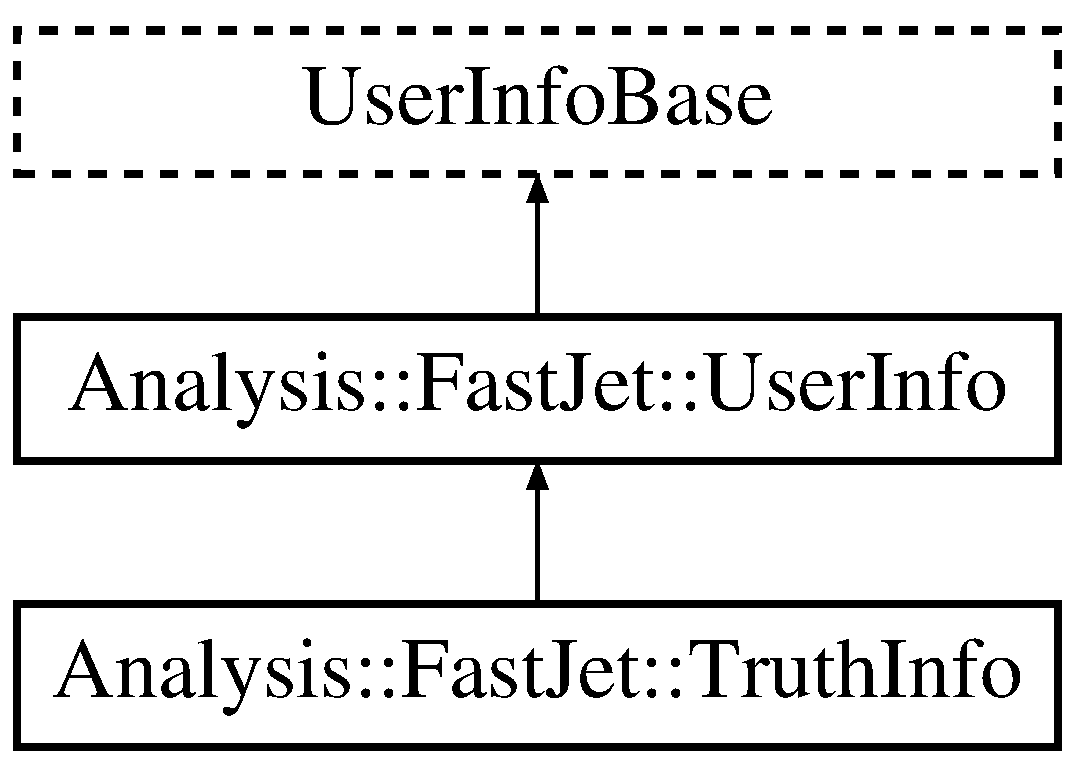
\includegraphics[height=3.000000cm]{classAnalysis_1_1FastJet_1_1TruthInfo}
\end{center}
\end{figure}
\subsection*{Public Member Functions}
\begin{DoxyCompactItemize}
\item 
\hyperlink{classAnalysis_1_1FastJet_1_1TruthInfo_a9f95f6e6557d67d77703a816fc913746}{Truth\+Info} ()
\item 
\hyperlink{classAnalysis_1_1FastJet_1_1TruthInfo_a983c57b1d61815b8e61e6debafc9a376}{Truth\+Info} (int idx, int \hyperlink{classAnalysis_1_1FastJet_1_1TruthInfo_ac1a7c34a77d7f0fc815ede73c35607ad}{pdg}, int \hyperlink{classAnalysis_1_1FastJet_1_1TruthInfo_a52a4e57c1e862882218f1e20ca9220c8}{status}, double \hyperlink{classAnalysis_1_1FastJet_1_1TruthInfo_a7d09bc00a310b2511bfc0ee4de23360c}{charge})
\item 
\hyperlink{classAnalysis_1_1FastJet_1_1TruthInfo_a0f0755f08f4cd85e21e646b0fbd6e47d}{Truth\+Info} (const \hyperlink{classAnalysis_1_1FastJet_1_1TruthInfo}{Truth\+Info} \&ti)
\item 
virtual \hyperlink{classAnalysis_1_1FastJet_1_1TruthInfo_a62a6d53a837ff38df9f7a7328bfb4d45}{$\sim$\+Truth\+Info} ()
\item 
int \hyperlink{classAnalysis_1_1FastJet_1_1TruthInfo_ac1a7c34a77d7f0fc815ede73c35607ad}{pdg} () const 
\item 
int \hyperlink{classAnalysis_1_1FastJet_1_1TruthInfo_a52a4e57c1e862882218f1e20ca9220c8}{status} () const 
\item 
double \hyperlink{classAnalysis_1_1FastJet_1_1TruthInfo_a7d09bc00a310b2511bfc0ee4de23360c}{charge} () const 
\item 
bool \hyperlink{classAnalysis_1_1FastJet_1_1TruthInfo_a1cdab47e0a01229a93aeebdbfbc4a993}{is\+Lepton} () const 
\item 
bool \hyperlink{classAnalysis_1_1FastJet_1_1TruthInfo_ac6f4703af5217047f0bc92f7853068a4}{is\+Hadron} () const 
\item 
bool \hyperlink{classAnalysis_1_1FastJet_1_1TruthInfo_a87297aa11e7f43dd729cdb709406a4d5}{is\+Neutrino} () const 
\item 
bool \hyperlink{classAnalysis_1_1FastJet_1_1TruthInfo_a1b994926fce41dc264134f1e61bdef00}{is\+Charged} () const 
\item 
bool \hyperlink{classAnalysis_1_1FastJet_1_1TruthInfo_a4edb489e915f6fcd967e8aa5b08b1027}{is\+Neutral} () const 
\end{DoxyCompactItemize}
\begin{Indent}{\bf Set object status}\par
{\em Set status to \char`\"{}empty\char`\"{} (no reference data) }\begin{DoxyCompactItemize}
\item 
virtual void \hyperlink{classAnalysis_1_1FastJet_1_1UserInfo_ab87ca9e42c15c24c8f54bad4b9674d0c}{set\+Empty} ()
\begin{DoxyCompactList}\small\item\em Set status to \char`\"{}faulty\char`\"{} (broken/invalid) \end{DoxyCompactList}\item 
virtual void \hyperlink{classAnalysis_1_1FastJet_1_1UserInfo_a0c5efdcfb658e75538dd5ec29c27afe0}{set\+Faulty} ()
\begin{DoxyCompactList}\small\item\em Set status to \char`\"{}faulty\char`\"{} (broken/invalid) \end{DoxyCompactList}\item 
virtual void \hyperlink{classAnalysis_1_1FastJet_1_1UserInfo_ab22ff88713e1ad12bd2311cc4f1c998c}{set\+Ghost} ()
\begin{DoxyCompactList}\small\item\em Set status to \char`\"{}ghosted\char`\"{}. \end{DoxyCompactList}\end{DoxyCompactItemize}
\end{Indent}
\begin{Indent}{\bf Access object status and data}\par
{\em Retrieve reference index (or status indicator)

\begin{DoxyReturn}{Returns}
Reference index if $>$= 0 (may still be invalid -\/ no checking); if $<$0 returns status. 
\end{DoxyReturn}
}\begin{DoxyCompactItemize}
\item 
virtual int \hyperlink{classAnalysis_1_1FastJet_1_1UserInfo_a687e6a814e58e5737108ef24aef047df}{index} () const 
\begin{DoxyCompactList}\small\item\em Check if empty. \end{DoxyCompactList}\item 
virtual bool \hyperlink{classAnalysis_1_1FastJet_1_1UserInfo_a4b987d1bba6c854cf9310596abbd3572}{is\+Empty} () const 
\begin{DoxyCompactList}\small\item\em Check if empty. \end{DoxyCompactList}\item 
virtual bool \hyperlink{classAnalysis_1_1FastJet_1_1UserInfo_a74601c143cb58b3bb62e0842b416beed}{is\+Faulty} () const 
\begin{DoxyCompactList}\small\item\em Check if faulty/broken/invalid. \end{DoxyCompactList}\item 
virtual bool \hyperlink{classAnalysis_1_1FastJet_1_1UserInfo_ad7b1ceba9d2ab04e7e7000577fe95198}{is\+Usable} () const 
\begin{DoxyCompactList}\small\item\em Check if usable. \end{DoxyCompactList}\item 
virtual bool \hyperlink{classAnalysis_1_1FastJet_1_1UserInfo_a92d2abe359ed4b794c546a23a9e1ccbe}{is\+Ghost} () const 
\begin{DoxyCompactList}\small\item\em Check if ghost. \end{DoxyCompactList}\end{DoxyCompactItemize}
\end{Indent}
\subsection*{Static Public Member Functions}
\begin{DoxyCompactItemize}
\item 
static bool \hyperlink{classAnalysis_1_1FastJet_1_1TruthInfo_a62a082245c4c8d8d370c7087de193dd4}{is\+Truth\+Particle} (const fastjet\+::\+Pseudo\+Jet \&pj)
\item 
static int \hyperlink{classAnalysis_1_1FastJet_1_1TruthInfo_ae1c07a279249c17a4d23c332291db118}{pdg} (const fastjet\+::\+Pseudo\+Jet \&pj)
\item 
static int \hyperlink{classAnalysis_1_1FastJet_1_1TruthInfo_ac12a01abd7648c60dd46f555c9c1a80d}{status} (const fastjet\+::\+Pseudo\+Jet \&pj)
\item 
static double \hyperlink{classAnalysis_1_1FastJet_1_1TruthInfo_af2cae2b143b988d8df611b0b66c744e2}{charge} (const fastjet\+::\+Pseudo\+Jet \&pj)
\item 
static bool \hyperlink{classAnalysis_1_1FastJet_1_1TruthInfo_a4444f96f6c8fe5ff215cff9d9ca34415}{is\+Hadron} (const fastjet\+::\+Pseudo\+Jet \&pj)
\item 
static bool \hyperlink{classAnalysis_1_1FastJet_1_1TruthInfo_a872fd6a63380813b5cbfac09372c3057}{is\+Lepton} (const fastjet\+::\+Pseudo\+Jet \&pj)
\item 
static bool \hyperlink{classAnalysis_1_1FastJet_1_1TruthInfo_a223902efb31a681c06d507ff6971c95b}{is\+Neutrino} (const fastjet\+::\+Pseudo\+Jet \&pj)
\item 
static bool \hyperlink{classAnalysis_1_1FastJet_1_1TruthInfo_a0c53d9c724ca822ec93efa84fcfbbafd}{is\+Charged} (const fastjet\+::\+Pseudo\+Jet \&pj)
\item 
static bool \hyperlink{classAnalysis_1_1FastJet_1_1TruthInfo_a41b32998acd985a82b5da1928b9723b7}{is\+Neutral} (const fastjet\+::\+Pseudo\+Jet \&pj)
\item 
static bool \hyperlink{classAnalysis_1_1FastJet_1_1UserInfo_a79ba59c5af9a4bc2e641ab2e54e8d50b}{is\+Empty} (const fastjet\+::\+Pseudo\+Jet \&pj)
\item 
static bool \hyperlink{classAnalysis_1_1FastJet_1_1UserInfo_a18b23aae344587ff280a046e70af1d29}{is\+Usable} (const fastjet\+::\+Pseudo\+Jet \&pj)
\item 
static bool \hyperlink{classAnalysis_1_1FastJet_1_1UserInfo_a4682fdc7e258328293b05951f55cc7a1}{is\+Ghost} (const fastjet\+::\+Pseudo\+Jet \&pj)
\item 
static bool \hyperlink{classAnalysis_1_1FastJet_1_1UserInfo_a681f1076b15320ea55e7104b4fe01c3a}{has\+User\+Info} (const fastjet\+::\+Pseudo\+Jet \&pj)
\item 
static int \hyperlink{classAnalysis_1_1FastJet_1_1UserInfo_a767f93f891d045f209198cdf72fddf36}{user\+Index} (const fastjet\+::\+Pseudo\+Jet \&pj)
\end{DoxyCompactItemize}
\subsection*{Protected Attributes}
\begin{DoxyCompactItemize}
\item 
int \hyperlink{classAnalysis_1_1FastJet_1_1TruthInfo_a667df4369792991c7882f89bc120e3e1}{\+\_\+pdg}
\item 
int \hyperlink{classAnalysis_1_1FastJet_1_1TruthInfo_a9da9ba4c65c112317584823af4de0bd7}{\+\_\+status}
\item 
double \hyperlink{classAnalysis_1_1FastJet_1_1TruthInfo_a44a9ca75492ca6e4e788e559f9afb1e7}{\+\_\+charge}
\item 
bool \hyperlink{classAnalysis_1_1FastJet_1_1TruthInfo_a3a86cf67d7da9be46ccd842723a75bcb}{\+\_\+is\+Hadron}
\item 
bool \hyperlink{classAnalysis_1_1FastJet_1_1TruthInfo_afa94b750c98dede7d4fa6a48c459dd5d}{\+\_\+is\+Lepton}
\item 
bool \hyperlink{classAnalysis_1_1FastJet_1_1TruthInfo_a18a62f405e19e57214a4ca36f815a2a0}{\+\_\+is\+Neutrino}
\item 
int \hyperlink{classAnalysis_1_1FastJet_1_1UserInfo_ad9aa33e317aea2b675493b664cc718a3}{\+\_\+idx}
\begin{DoxyCompactList}\small\item\em Index to underlying structure holding data. \end{DoxyCompactList}\end{DoxyCompactItemize}
\subsection*{Static Private Attributes}
\begin{DoxyCompactItemize}
\item 
static const std\+::vector$<$ int $>$ \hyperlink{classAnalysis_1_1FastJet_1_1TruthInfo_a23c0cd8c38cbc6613aafb00170365437}{\+\_\+leptons} = \{ 11, -\/11, 13, -\/13, 15, -\/15, 17, -\/17 \}
\item 
static const std\+::vector$<$ int $>$ \hyperlink{classAnalysis_1_1FastJet_1_1TruthInfo_a79f2101d71790e8f4a9bbb42843b3c26}{\+\_\+neutrinos} = \{ 12, -\/12, 14, -\/14, 16, -\/16, 18, -\/18 \}
\end{DoxyCompactItemize}


\subsection{Detailed Description}


Definition at line 492 of file Analysis\+Data.\+h.



\subsection{Constructor \& Destructor Documentation}
\index{Analysis\+::\+Fast\+Jet\+::\+Truth\+Info@{Analysis\+::\+Fast\+Jet\+::\+Truth\+Info}!Truth\+Info@{Truth\+Info}}
\index{Truth\+Info@{Truth\+Info}!Analysis\+::\+Fast\+Jet\+::\+Truth\+Info@{Analysis\+::\+Fast\+Jet\+::\+Truth\+Info}}
\subsubsection[{\texorpdfstring{Truth\+Info()}{TruthInfo()}}]{\setlength{\rightskip}{0pt plus 5cm}Analysis\+::\+Fast\+Jet\+::\+Truth\+Info\+::\+Truth\+Info (
\begin{DoxyParamCaption}
{}
\end{DoxyParamCaption}
)\hspace{0.3cm}{\ttfamily [inline]}}\hypertarget{classAnalysis_1_1FastJet_1_1TruthInfo_a9f95f6e6557d67d77703a816fc913746}{}\label{classAnalysis_1_1FastJet_1_1TruthInfo_a9f95f6e6557d67d77703a816fc913746}


Definition at line 505 of file Analysis\+Data.\+h.

\index{Analysis\+::\+Fast\+Jet\+::\+Truth\+Info@{Analysis\+::\+Fast\+Jet\+::\+Truth\+Info}!Truth\+Info@{Truth\+Info}}
\index{Truth\+Info@{Truth\+Info}!Analysis\+::\+Fast\+Jet\+::\+Truth\+Info@{Analysis\+::\+Fast\+Jet\+::\+Truth\+Info}}
\subsubsection[{\texorpdfstring{Truth\+Info(int idx, int pdg, int status, double charge)}{TruthInfo(int idx, int pdg, int status, double charge)}}]{\setlength{\rightskip}{0pt plus 5cm}Analysis\+::\+Fast\+Jet\+::\+Truth\+Info\+::\+Truth\+Info (
\begin{DoxyParamCaption}
\item[{int}]{idx, }
\item[{int}]{pdg, }
\item[{int}]{status, }
\item[{double}]{charge}
\end{DoxyParamCaption}
)\hspace{0.3cm}{\ttfamily [inline]}}\hypertarget{classAnalysis_1_1FastJet_1_1TruthInfo_a983c57b1d61815b8e61e6debafc9a376}{}\label{classAnalysis_1_1FastJet_1_1TruthInfo_a983c57b1d61815b8e61e6debafc9a376}


Definition at line 514 of file Analysis\+Data.\+h.

\index{Analysis\+::\+Fast\+Jet\+::\+Truth\+Info@{Analysis\+::\+Fast\+Jet\+::\+Truth\+Info}!Truth\+Info@{Truth\+Info}}
\index{Truth\+Info@{Truth\+Info}!Analysis\+::\+Fast\+Jet\+::\+Truth\+Info@{Analysis\+::\+Fast\+Jet\+::\+Truth\+Info}}
\subsubsection[{\texorpdfstring{Truth\+Info(const Truth\+Info \&ti)}{TruthInfo(const TruthInfo &ti)}}]{\setlength{\rightskip}{0pt plus 5cm}Analysis\+::\+Fast\+Jet\+::\+Truth\+Info\+::\+Truth\+Info (
\begin{DoxyParamCaption}
\item[{const {\bf Truth\+Info} \&}]{ti}
\end{DoxyParamCaption}
)\hspace{0.3cm}{\ttfamily [inline]}}\hypertarget{classAnalysis_1_1FastJet_1_1TruthInfo_a0f0755f08f4cd85e21e646b0fbd6e47d}{}\label{classAnalysis_1_1FastJet_1_1TruthInfo_a0f0755f08f4cd85e21e646b0fbd6e47d}


Definition at line 530 of file Analysis\+Data.\+h.

\index{Analysis\+::\+Fast\+Jet\+::\+Truth\+Info@{Analysis\+::\+Fast\+Jet\+::\+Truth\+Info}!````~Truth\+Info@{$\sim$\+Truth\+Info}}
\index{````~Truth\+Info@{$\sim$\+Truth\+Info}!Analysis\+::\+Fast\+Jet\+::\+Truth\+Info@{Analysis\+::\+Fast\+Jet\+::\+Truth\+Info}}
\subsubsection[{\texorpdfstring{$\sim$\+Truth\+Info()}{~TruthInfo()}}]{\setlength{\rightskip}{0pt plus 5cm}virtual Analysis\+::\+Fast\+Jet\+::\+Truth\+Info\+::$\sim$\+Truth\+Info (
\begin{DoxyParamCaption}
{}
\end{DoxyParamCaption}
)\hspace{0.3cm}{\ttfamily [inline]}, {\ttfamily [virtual]}}\hypertarget{classAnalysis_1_1FastJet_1_1TruthInfo_a62a6d53a837ff38df9f7a7328bfb4d45}{}\label{classAnalysis_1_1FastJet_1_1TruthInfo_a62a6d53a837ff38df9f7a7328bfb4d45}


Definition at line 539 of file Analysis\+Data.\+h.



\subsection{Member Function Documentation}
\index{Analysis\+::\+Fast\+Jet\+::\+Truth\+Info@{Analysis\+::\+Fast\+Jet\+::\+Truth\+Info}!charge@{charge}}
\index{charge@{charge}!Analysis\+::\+Fast\+Jet\+::\+Truth\+Info@{Analysis\+::\+Fast\+Jet\+::\+Truth\+Info}}
\subsubsection[{\texorpdfstring{charge() const }{charge() const }}]{\setlength{\rightskip}{0pt plus 5cm}double Analysis\+::\+Fast\+Jet\+::\+Truth\+Info\+::charge (
\begin{DoxyParamCaption}
{}
\end{DoxyParamCaption}
) const\hspace{0.3cm}{\ttfamily [inline]}}\hypertarget{classAnalysis_1_1FastJet_1_1TruthInfo_a7d09bc00a310b2511bfc0ee4de23360c}{}\label{classAnalysis_1_1FastJet_1_1TruthInfo_a7d09bc00a310b2511bfc0ee4de23360c}


Definition at line 542 of file Analysis\+Data.\+h.

\index{Analysis\+::\+Fast\+Jet\+::\+Truth\+Info@{Analysis\+::\+Fast\+Jet\+::\+Truth\+Info}!charge@{charge}}
\index{charge@{charge}!Analysis\+::\+Fast\+Jet\+::\+Truth\+Info@{Analysis\+::\+Fast\+Jet\+::\+Truth\+Info}}
\subsubsection[{\texorpdfstring{charge(const fastjet\+::\+Pseudo\+Jet \&pj)}{charge(const fastjet::PseudoJet &pj)}}]{\setlength{\rightskip}{0pt plus 5cm}static double Analysis\+::\+Fast\+Jet\+::\+Truth\+Info\+::charge (
\begin{DoxyParamCaption}
\item[{const fastjet\+::\+Pseudo\+Jet \&}]{pj}
\end{DoxyParamCaption}
)\hspace{0.3cm}{\ttfamily [inline]}, {\ttfamily [static]}}\hypertarget{classAnalysis_1_1FastJet_1_1TruthInfo_af2cae2b143b988d8df611b0b66c744e2}{}\label{classAnalysis_1_1FastJet_1_1TruthInfo_af2cae2b143b988d8df611b0b66c744e2}


Definition at line 556 of file Analysis\+Data.\+h.

\index{Analysis\+::\+Fast\+Jet\+::\+Truth\+Info@{Analysis\+::\+Fast\+Jet\+::\+Truth\+Info}!has\+User\+Info@{has\+User\+Info}}
\index{has\+User\+Info@{has\+User\+Info}!Analysis\+::\+Fast\+Jet\+::\+Truth\+Info@{Analysis\+::\+Fast\+Jet\+::\+Truth\+Info}}
\subsubsection[{\texorpdfstring{has\+User\+Info(const fastjet\+::\+Pseudo\+Jet \&pj)}{hasUserInfo(const fastjet::PseudoJet &pj)}}]{\setlength{\rightskip}{0pt plus 5cm}static bool Analysis\+::\+Fast\+Jet\+::\+User\+Info\+::has\+User\+Info (
\begin{DoxyParamCaption}
\item[{const fastjet\+::\+Pseudo\+Jet \&}]{pj}
\end{DoxyParamCaption}
)\hspace{0.3cm}{\ttfamily [inline]}, {\ttfamily [static]}, {\ttfamily [inherited]}}\hypertarget{classAnalysis_1_1FastJet_1_1UserInfo_a681f1076b15320ea55e7104b4fe01c3a}{}\label{classAnalysis_1_1FastJet_1_1UserInfo_a681f1076b15320ea55e7104b4fe01c3a}


Definition at line 357 of file Analysis\+Data.\+h.

\index{Analysis\+::\+Fast\+Jet\+::\+Truth\+Info@{Analysis\+::\+Fast\+Jet\+::\+Truth\+Info}!index@{index}}
\index{index@{index}!Analysis\+::\+Fast\+Jet\+::\+Truth\+Info@{Analysis\+::\+Fast\+Jet\+::\+Truth\+Info}}
\subsubsection[{\texorpdfstring{index() const }{index() const }}]{\setlength{\rightskip}{0pt plus 5cm}virtual int Analysis\+::\+Fast\+Jet\+::\+User\+Info\+::index (
\begin{DoxyParamCaption}
{}
\end{DoxyParamCaption}
) const\hspace{0.3cm}{\ttfamily [inline]}, {\ttfamily [virtual]}, {\ttfamily [inherited]}}\hypertarget{classAnalysis_1_1FastJet_1_1UserInfo_a687e6a814e58e5737108ef24aef047df}{}\label{classAnalysis_1_1FastJet_1_1UserInfo_a687e6a814e58e5737108ef24aef047df}


Check if empty. 

\begin{DoxyReturn}{Returns}
{\ttfamily true} if empty. 
\end{DoxyReturn}


Definition at line 338 of file Analysis\+Data.\+h.

\index{Analysis\+::\+Fast\+Jet\+::\+Truth\+Info@{Analysis\+::\+Fast\+Jet\+::\+Truth\+Info}!is\+Charged@{is\+Charged}}
\index{is\+Charged@{is\+Charged}!Analysis\+::\+Fast\+Jet\+::\+Truth\+Info@{Analysis\+::\+Fast\+Jet\+::\+Truth\+Info}}
\subsubsection[{\texorpdfstring{is\+Charged() const }{isCharged() const }}]{\setlength{\rightskip}{0pt plus 5cm}bool Analysis\+::\+Fast\+Jet\+::\+Truth\+Info\+::is\+Charged (
\begin{DoxyParamCaption}
{}
\end{DoxyParamCaption}
) const\hspace{0.3cm}{\ttfamily [inline]}}\hypertarget{classAnalysis_1_1FastJet_1_1TruthInfo_a1b994926fce41dc264134f1e61bdef00}{}\label{classAnalysis_1_1FastJet_1_1TruthInfo_a1b994926fce41dc264134f1e61bdef00}


Definition at line 546 of file Analysis\+Data.\+h.

\index{Analysis\+::\+Fast\+Jet\+::\+Truth\+Info@{Analysis\+::\+Fast\+Jet\+::\+Truth\+Info}!is\+Charged@{is\+Charged}}
\index{is\+Charged@{is\+Charged}!Analysis\+::\+Fast\+Jet\+::\+Truth\+Info@{Analysis\+::\+Fast\+Jet\+::\+Truth\+Info}}
\subsubsection[{\texorpdfstring{is\+Charged(const fastjet\+::\+Pseudo\+Jet \&pj)}{isCharged(const fastjet::PseudoJet &pj)}}]{\setlength{\rightskip}{0pt plus 5cm}static bool Analysis\+::\+Fast\+Jet\+::\+Truth\+Info\+::is\+Charged (
\begin{DoxyParamCaption}
\item[{const fastjet\+::\+Pseudo\+Jet \&}]{pj}
\end{DoxyParamCaption}
)\hspace{0.3cm}{\ttfamily [inline]}, {\ttfamily [static]}}\hypertarget{classAnalysis_1_1FastJet_1_1TruthInfo_a0c53d9c724ca822ec93efa84fcfbbafd}{}\label{classAnalysis_1_1FastJet_1_1TruthInfo_a0c53d9c724ca822ec93efa84fcfbbafd}


Definition at line 564 of file Analysis\+Data.\+h.

\index{Analysis\+::\+Fast\+Jet\+::\+Truth\+Info@{Analysis\+::\+Fast\+Jet\+::\+Truth\+Info}!is\+Empty@{is\+Empty}}
\index{is\+Empty@{is\+Empty}!Analysis\+::\+Fast\+Jet\+::\+Truth\+Info@{Analysis\+::\+Fast\+Jet\+::\+Truth\+Info}}
\subsubsection[{\texorpdfstring{is\+Empty() const }{isEmpty() const }}]{\setlength{\rightskip}{0pt plus 5cm}virtual bool Analysis\+::\+Fast\+Jet\+::\+User\+Info\+::is\+Empty (
\begin{DoxyParamCaption}
{}
\end{DoxyParamCaption}
) const\hspace{0.3cm}{\ttfamily [inline]}, {\ttfamily [virtual]}, {\ttfamily [inherited]}}\hypertarget{classAnalysis_1_1FastJet_1_1UserInfo_a4b987d1bba6c854cf9310596abbd3572}{}\label{classAnalysis_1_1FastJet_1_1UserInfo_a4b987d1bba6c854cf9310596abbd3572}


Check if empty. 

\begin{DoxyReturn}{Returns}
{\ttfamily true} if empty. 
\end{DoxyReturn}


Definition at line 342 of file Analysis\+Data.\+h.

\index{Analysis\+::\+Fast\+Jet\+::\+Truth\+Info@{Analysis\+::\+Fast\+Jet\+::\+Truth\+Info}!is\+Empty@{is\+Empty}}
\index{is\+Empty@{is\+Empty}!Analysis\+::\+Fast\+Jet\+::\+Truth\+Info@{Analysis\+::\+Fast\+Jet\+::\+Truth\+Info}}
\subsubsection[{\texorpdfstring{is\+Empty(const fastjet\+::\+Pseudo\+Jet \&pj)}{isEmpty(const fastjet::PseudoJet &pj)}}]{\setlength{\rightskip}{0pt plus 5cm}static bool Analysis\+::\+Fast\+Jet\+::\+User\+Info\+::is\+Empty (
\begin{DoxyParamCaption}
\item[{const fastjet\+::\+Pseudo\+Jet \&}]{pj}
\end{DoxyParamCaption}
)\hspace{0.3cm}{\ttfamily [inline]}, {\ttfamily [static]}, {\ttfamily [inherited]}}\hypertarget{classAnalysis_1_1FastJet_1_1UserInfo_a79ba59c5af9a4bc2e641ab2e54e8d50b}{}\label{classAnalysis_1_1FastJet_1_1UserInfo_a79ba59c5af9a4bc2e641ab2e54e8d50b}


Definition at line 362 of file Analysis\+Data.\+h.

\index{Analysis\+::\+Fast\+Jet\+::\+Truth\+Info@{Analysis\+::\+Fast\+Jet\+::\+Truth\+Info}!is\+Faulty@{is\+Faulty}}
\index{is\+Faulty@{is\+Faulty}!Analysis\+::\+Fast\+Jet\+::\+Truth\+Info@{Analysis\+::\+Fast\+Jet\+::\+Truth\+Info}}
\subsubsection[{\texorpdfstring{is\+Faulty() const }{isFaulty() const }}]{\setlength{\rightskip}{0pt plus 5cm}virtual bool Analysis\+::\+Fast\+Jet\+::\+User\+Info\+::is\+Faulty (
\begin{DoxyParamCaption}
{}
\end{DoxyParamCaption}
) const\hspace{0.3cm}{\ttfamily [inline]}, {\ttfamily [virtual]}, {\ttfamily [inherited]}}\hypertarget{classAnalysis_1_1FastJet_1_1UserInfo_a74601c143cb58b3bb62e0842b416beed}{}\label{classAnalysis_1_1FastJet_1_1UserInfo_a74601c143cb58b3bb62e0842b416beed}


Check if faulty/broken/invalid. 

\begin{DoxyReturn}{Returns}
{\ttfamily true} if faulty. 
\end{DoxyReturn}


Definition at line 346 of file Analysis\+Data.\+h.

\index{Analysis\+::\+Fast\+Jet\+::\+Truth\+Info@{Analysis\+::\+Fast\+Jet\+::\+Truth\+Info}!is\+Ghost@{is\+Ghost}}
\index{is\+Ghost@{is\+Ghost}!Analysis\+::\+Fast\+Jet\+::\+Truth\+Info@{Analysis\+::\+Fast\+Jet\+::\+Truth\+Info}}
\subsubsection[{\texorpdfstring{is\+Ghost() const }{isGhost() const }}]{\setlength{\rightskip}{0pt plus 5cm}virtual bool Analysis\+::\+Fast\+Jet\+::\+User\+Info\+::is\+Ghost (
\begin{DoxyParamCaption}
{}
\end{DoxyParamCaption}
) const\hspace{0.3cm}{\ttfamily [inline]}, {\ttfamily [virtual]}, {\ttfamily [inherited]}}\hypertarget{classAnalysis_1_1FastJet_1_1UserInfo_a92d2abe359ed4b794c546a23a9e1ccbe}{}\label{classAnalysis_1_1FastJet_1_1UserInfo_a92d2abe359ed4b794c546a23a9e1ccbe}


Check if ghost. 

\begin{DoxyReturn}{Returns}
{\ttfamily true} of associated {\ttfamily fastjet\+::\+Pseudo\+Jet} is ghosted 
\end{DoxyReturn}


Definition at line 354 of file Analysis\+Data.\+h.

\index{Analysis\+::\+Fast\+Jet\+::\+Truth\+Info@{Analysis\+::\+Fast\+Jet\+::\+Truth\+Info}!is\+Ghost@{is\+Ghost}}
\index{is\+Ghost@{is\+Ghost}!Analysis\+::\+Fast\+Jet\+::\+Truth\+Info@{Analysis\+::\+Fast\+Jet\+::\+Truth\+Info}}
\subsubsection[{\texorpdfstring{is\+Ghost(const fastjet\+::\+Pseudo\+Jet \&pj)}{isGhost(const fastjet::PseudoJet &pj)}}]{\setlength{\rightskip}{0pt plus 5cm}static bool Analysis\+::\+Fast\+Jet\+::\+User\+Info\+::is\+Ghost (
\begin{DoxyParamCaption}
\item[{const fastjet\+::\+Pseudo\+Jet \&}]{pj}
\end{DoxyParamCaption}
)\hspace{0.3cm}{\ttfamily [inline]}, {\ttfamily [static]}, {\ttfamily [inherited]}}\hypertarget{classAnalysis_1_1FastJet_1_1UserInfo_a4682fdc7e258328293b05951f55cc7a1}{}\label{classAnalysis_1_1FastJet_1_1UserInfo_a4682fdc7e258328293b05951f55cc7a1}


Definition at line 366 of file Analysis\+Data.\+h.

\index{Analysis\+::\+Fast\+Jet\+::\+Truth\+Info@{Analysis\+::\+Fast\+Jet\+::\+Truth\+Info}!is\+Hadron@{is\+Hadron}}
\index{is\+Hadron@{is\+Hadron}!Analysis\+::\+Fast\+Jet\+::\+Truth\+Info@{Analysis\+::\+Fast\+Jet\+::\+Truth\+Info}}
\subsubsection[{\texorpdfstring{is\+Hadron() const }{isHadron() const }}]{\setlength{\rightskip}{0pt plus 5cm}bool Analysis\+::\+Fast\+Jet\+::\+Truth\+Info\+::is\+Hadron (
\begin{DoxyParamCaption}
{}
\end{DoxyParamCaption}
) const\hspace{0.3cm}{\ttfamily [inline]}}\hypertarget{classAnalysis_1_1FastJet_1_1TruthInfo_ac6f4703af5217047f0bc92f7853068a4}{}\label{classAnalysis_1_1FastJet_1_1TruthInfo_ac6f4703af5217047f0bc92f7853068a4}


Definition at line 544 of file Analysis\+Data.\+h.

\index{Analysis\+::\+Fast\+Jet\+::\+Truth\+Info@{Analysis\+::\+Fast\+Jet\+::\+Truth\+Info}!is\+Hadron@{is\+Hadron}}
\index{is\+Hadron@{is\+Hadron}!Analysis\+::\+Fast\+Jet\+::\+Truth\+Info@{Analysis\+::\+Fast\+Jet\+::\+Truth\+Info}}
\subsubsection[{\texorpdfstring{is\+Hadron(const fastjet\+::\+Pseudo\+Jet \&pj)}{isHadron(const fastjet::PseudoJet &pj)}}]{\setlength{\rightskip}{0pt plus 5cm}static bool Analysis\+::\+Fast\+Jet\+::\+Truth\+Info\+::is\+Hadron (
\begin{DoxyParamCaption}
\item[{const fastjet\+::\+Pseudo\+Jet \&}]{pj}
\end{DoxyParamCaption}
)\hspace{0.3cm}{\ttfamily [inline]}, {\ttfamily [static]}}\hypertarget{classAnalysis_1_1FastJet_1_1TruthInfo_a4444f96f6c8fe5ff215cff9d9ca34415}{}\label{classAnalysis_1_1FastJet_1_1TruthInfo_a4444f96f6c8fe5ff215cff9d9ca34415}


Definition at line 558 of file Analysis\+Data.\+h.

\index{Analysis\+::\+Fast\+Jet\+::\+Truth\+Info@{Analysis\+::\+Fast\+Jet\+::\+Truth\+Info}!is\+Lepton@{is\+Lepton}}
\index{is\+Lepton@{is\+Lepton}!Analysis\+::\+Fast\+Jet\+::\+Truth\+Info@{Analysis\+::\+Fast\+Jet\+::\+Truth\+Info}}
\subsubsection[{\texorpdfstring{is\+Lepton() const }{isLepton() const }}]{\setlength{\rightskip}{0pt plus 5cm}bool Analysis\+::\+Fast\+Jet\+::\+Truth\+Info\+::is\+Lepton (
\begin{DoxyParamCaption}
{}
\end{DoxyParamCaption}
) const\hspace{0.3cm}{\ttfamily [inline]}}\hypertarget{classAnalysis_1_1FastJet_1_1TruthInfo_a1cdab47e0a01229a93aeebdbfbc4a993}{}\label{classAnalysis_1_1FastJet_1_1TruthInfo_a1cdab47e0a01229a93aeebdbfbc4a993}


Definition at line 543 of file Analysis\+Data.\+h.

\index{Analysis\+::\+Fast\+Jet\+::\+Truth\+Info@{Analysis\+::\+Fast\+Jet\+::\+Truth\+Info}!is\+Lepton@{is\+Lepton}}
\index{is\+Lepton@{is\+Lepton}!Analysis\+::\+Fast\+Jet\+::\+Truth\+Info@{Analysis\+::\+Fast\+Jet\+::\+Truth\+Info}}
\subsubsection[{\texorpdfstring{is\+Lepton(const fastjet\+::\+Pseudo\+Jet \&pj)}{isLepton(const fastjet::PseudoJet &pj)}}]{\setlength{\rightskip}{0pt plus 5cm}static bool Analysis\+::\+Fast\+Jet\+::\+Truth\+Info\+::is\+Lepton (
\begin{DoxyParamCaption}
\item[{const fastjet\+::\+Pseudo\+Jet \&}]{pj}
\end{DoxyParamCaption}
)\hspace{0.3cm}{\ttfamily [inline]}, {\ttfamily [static]}}\hypertarget{classAnalysis_1_1FastJet_1_1TruthInfo_a872fd6a63380813b5cbfac09372c3057}{}\label{classAnalysis_1_1FastJet_1_1TruthInfo_a872fd6a63380813b5cbfac09372c3057}


Definition at line 560 of file Analysis\+Data.\+h.

\index{Analysis\+::\+Fast\+Jet\+::\+Truth\+Info@{Analysis\+::\+Fast\+Jet\+::\+Truth\+Info}!is\+Neutral@{is\+Neutral}}
\index{is\+Neutral@{is\+Neutral}!Analysis\+::\+Fast\+Jet\+::\+Truth\+Info@{Analysis\+::\+Fast\+Jet\+::\+Truth\+Info}}
\subsubsection[{\texorpdfstring{is\+Neutral() const }{isNeutral() const }}]{\setlength{\rightskip}{0pt plus 5cm}bool Analysis\+::\+Fast\+Jet\+::\+Truth\+Info\+::is\+Neutral (
\begin{DoxyParamCaption}
{}
\end{DoxyParamCaption}
) const\hspace{0.3cm}{\ttfamily [inline]}}\hypertarget{classAnalysis_1_1FastJet_1_1TruthInfo_a4edb489e915f6fcd967e8aa5b08b1027}{}\label{classAnalysis_1_1FastJet_1_1TruthInfo_a4edb489e915f6fcd967e8aa5b08b1027}


Definition at line 547 of file Analysis\+Data.\+h.

\index{Analysis\+::\+Fast\+Jet\+::\+Truth\+Info@{Analysis\+::\+Fast\+Jet\+::\+Truth\+Info}!is\+Neutral@{is\+Neutral}}
\index{is\+Neutral@{is\+Neutral}!Analysis\+::\+Fast\+Jet\+::\+Truth\+Info@{Analysis\+::\+Fast\+Jet\+::\+Truth\+Info}}
\subsubsection[{\texorpdfstring{is\+Neutral(const fastjet\+::\+Pseudo\+Jet \&pj)}{isNeutral(const fastjet::PseudoJet &pj)}}]{\setlength{\rightskip}{0pt plus 5cm}static bool Analysis\+::\+Fast\+Jet\+::\+Truth\+Info\+::is\+Neutral (
\begin{DoxyParamCaption}
\item[{const fastjet\+::\+Pseudo\+Jet \&}]{pj}
\end{DoxyParamCaption}
)\hspace{0.3cm}{\ttfamily [inline]}, {\ttfamily [static]}}\hypertarget{classAnalysis_1_1FastJet_1_1TruthInfo_a41b32998acd985a82b5da1928b9723b7}{}\label{classAnalysis_1_1FastJet_1_1TruthInfo_a41b32998acd985a82b5da1928b9723b7}


Definition at line 566 of file Analysis\+Data.\+h.

\index{Analysis\+::\+Fast\+Jet\+::\+Truth\+Info@{Analysis\+::\+Fast\+Jet\+::\+Truth\+Info}!is\+Neutrino@{is\+Neutrino}}
\index{is\+Neutrino@{is\+Neutrino}!Analysis\+::\+Fast\+Jet\+::\+Truth\+Info@{Analysis\+::\+Fast\+Jet\+::\+Truth\+Info}}
\subsubsection[{\texorpdfstring{is\+Neutrino() const }{isNeutrino() const }}]{\setlength{\rightskip}{0pt plus 5cm}bool Analysis\+::\+Fast\+Jet\+::\+Truth\+Info\+::is\+Neutrino (
\begin{DoxyParamCaption}
{}
\end{DoxyParamCaption}
) const\hspace{0.3cm}{\ttfamily [inline]}}\hypertarget{classAnalysis_1_1FastJet_1_1TruthInfo_a87297aa11e7f43dd729cdb709406a4d5}{}\label{classAnalysis_1_1FastJet_1_1TruthInfo_a87297aa11e7f43dd729cdb709406a4d5}


Definition at line 545 of file Analysis\+Data.\+h.

\index{Analysis\+::\+Fast\+Jet\+::\+Truth\+Info@{Analysis\+::\+Fast\+Jet\+::\+Truth\+Info}!is\+Neutrino@{is\+Neutrino}}
\index{is\+Neutrino@{is\+Neutrino}!Analysis\+::\+Fast\+Jet\+::\+Truth\+Info@{Analysis\+::\+Fast\+Jet\+::\+Truth\+Info}}
\subsubsection[{\texorpdfstring{is\+Neutrino(const fastjet\+::\+Pseudo\+Jet \&pj)}{isNeutrino(const fastjet::PseudoJet &pj)}}]{\setlength{\rightskip}{0pt plus 5cm}static bool Analysis\+::\+Fast\+Jet\+::\+Truth\+Info\+::is\+Neutrino (
\begin{DoxyParamCaption}
\item[{const fastjet\+::\+Pseudo\+Jet \&}]{pj}
\end{DoxyParamCaption}
)\hspace{0.3cm}{\ttfamily [inline]}, {\ttfamily [static]}}\hypertarget{classAnalysis_1_1FastJet_1_1TruthInfo_a223902efb31a681c06d507ff6971c95b}{}\label{classAnalysis_1_1FastJet_1_1TruthInfo_a223902efb31a681c06d507ff6971c95b}


Definition at line 562 of file Analysis\+Data.\+h.

\index{Analysis\+::\+Fast\+Jet\+::\+Truth\+Info@{Analysis\+::\+Fast\+Jet\+::\+Truth\+Info}!is\+Truth\+Particle@{is\+Truth\+Particle}}
\index{is\+Truth\+Particle@{is\+Truth\+Particle}!Analysis\+::\+Fast\+Jet\+::\+Truth\+Info@{Analysis\+::\+Fast\+Jet\+::\+Truth\+Info}}
\subsubsection[{\texorpdfstring{is\+Truth\+Particle(const fastjet\+::\+Pseudo\+Jet \&pj)}{isTruthParticle(const fastjet::PseudoJet &pj)}}]{\setlength{\rightskip}{0pt plus 5cm}static bool Analysis\+::\+Fast\+Jet\+::\+Truth\+Info\+::is\+Truth\+Particle (
\begin{DoxyParamCaption}
\item[{const fastjet\+::\+Pseudo\+Jet \&}]{pj}
\end{DoxyParamCaption}
)\hspace{0.3cm}{\ttfamily [inline]}, {\ttfamily [static]}}\hypertarget{classAnalysis_1_1FastJet_1_1TruthInfo_a62a082245c4c8d8d370c7087de193dd4}{}\label{classAnalysis_1_1FastJet_1_1TruthInfo_a62a082245c4c8d8d370c7087de193dd4}


Definition at line 549 of file Analysis\+Data.\+h.

\index{Analysis\+::\+Fast\+Jet\+::\+Truth\+Info@{Analysis\+::\+Fast\+Jet\+::\+Truth\+Info}!is\+Usable@{is\+Usable}}
\index{is\+Usable@{is\+Usable}!Analysis\+::\+Fast\+Jet\+::\+Truth\+Info@{Analysis\+::\+Fast\+Jet\+::\+Truth\+Info}}
\subsubsection[{\texorpdfstring{is\+Usable() const }{isUsable() const }}]{\setlength{\rightskip}{0pt plus 5cm}virtual bool Analysis\+::\+Fast\+Jet\+::\+User\+Info\+::is\+Usable (
\begin{DoxyParamCaption}
{}
\end{DoxyParamCaption}
) const\hspace{0.3cm}{\ttfamily [inline]}, {\ttfamily [virtual]}, {\ttfamily [inherited]}}\hypertarget{classAnalysis_1_1FastJet_1_1UserInfo_ad7b1ceba9d2ab04e7e7000577fe95198}{}\label{classAnalysis_1_1FastJet_1_1UserInfo_ad7b1ceba9d2ab04e7e7000577fe95198}


Check if usable. 

\begin{DoxyReturn}{Returns}
{\ttfamily true} if usable -\/ no indication that the index is valid! 
\end{DoxyReturn}


Definition at line 350 of file Analysis\+Data.\+h.

\index{Analysis\+::\+Fast\+Jet\+::\+Truth\+Info@{Analysis\+::\+Fast\+Jet\+::\+Truth\+Info}!is\+Usable@{is\+Usable}}
\index{is\+Usable@{is\+Usable}!Analysis\+::\+Fast\+Jet\+::\+Truth\+Info@{Analysis\+::\+Fast\+Jet\+::\+Truth\+Info}}
\subsubsection[{\texorpdfstring{is\+Usable(const fastjet\+::\+Pseudo\+Jet \&pj)}{isUsable(const fastjet::PseudoJet &pj)}}]{\setlength{\rightskip}{0pt plus 5cm}static bool Analysis\+::\+Fast\+Jet\+::\+User\+Info\+::is\+Usable (
\begin{DoxyParamCaption}
\item[{const fastjet\+::\+Pseudo\+Jet \&}]{pj}
\end{DoxyParamCaption}
)\hspace{0.3cm}{\ttfamily [inline]}, {\ttfamily [static]}, {\ttfamily [inherited]}}\hypertarget{classAnalysis_1_1FastJet_1_1UserInfo_a18b23aae344587ff280a046e70af1d29}{}\label{classAnalysis_1_1FastJet_1_1UserInfo_a18b23aae344587ff280a046e70af1d29}


Definition at line 364 of file Analysis\+Data.\+h.

\index{Analysis\+::\+Fast\+Jet\+::\+Truth\+Info@{Analysis\+::\+Fast\+Jet\+::\+Truth\+Info}!pdg@{pdg}}
\index{pdg@{pdg}!Analysis\+::\+Fast\+Jet\+::\+Truth\+Info@{Analysis\+::\+Fast\+Jet\+::\+Truth\+Info}}
\subsubsection[{\texorpdfstring{pdg() const }{pdg() const }}]{\setlength{\rightskip}{0pt plus 5cm}int Analysis\+::\+Fast\+Jet\+::\+Truth\+Info\+::pdg (
\begin{DoxyParamCaption}
{}
\end{DoxyParamCaption}
) const\hspace{0.3cm}{\ttfamily [inline]}}\hypertarget{classAnalysis_1_1FastJet_1_1TruthInfo_ac1a7c34a77d7f0fc815ede73c35607ad}{}\label{classAnalysis_1_1FastJet_1_1TruthInfo_ac1a7c34a77d7f0fc815ede73c35607ad}


Definition at line 540 of file Analysis\+Data.\+h.

\index{Analysis\+::\+Fast\+Jet\+::\+Truth\+Info@{Analysis\+::\+Fast\+Jet\+::\+Truth\+Info}!pdg@{pdg}}
\index{pdg@{pdg}!Analysis\+::\+Fast\+Jet\+::\+Truth\+Info@{Analysis\+::\+Fast\+Jet\+::\+Truth\+Info}}
\subsubsection[{\texorpdfstring{pdg(const fastjet\+::\+Pseudo\+Jet \&pj)}{pdg(const fastjet::PseudoJet &pj)}}]{\setlength{\rightskip}{0pt plus 5cm}static int Analysis\+::\+Fast\+Jet\+::\+Truth\+Info\+::pdg (
\begin{DoxyParamCaption}
\item[{const fastjet\+::\+Pseudo\+Jet \&}]{pj}
\end{DoxyParamCaption}
)\hspace{0.3cm}{\ttfamily [inline]}, {\ttfamily [static]}}\hypertarget{classAnalysis_1_1FastJet_1_1TruthInfo_ae1c07a279249c17a4d23c332291db118}{}\label{classAnalysis_1_1FastJet_1_1TruthInfo_ae1c07a279249c17a4d23c332291db118}


Definition at line 552 of file Analysis\+Data.\+h.

\index{Analysis\+::\+Fast\+Jet\+::\+Truth\+Info@{Analysis\+::\+Fast\+Jet\+::\+Truth\+Info}!set\+Empty@{set\+Empty}}
\index{set\+Empty@{set\+Empty}!Analysis\+::\+Fast\+Jet\+::\+Truth\+Info@{Analysis\+::\+Fast\+Jet\+::\+Truth\+Info}}
\subsubsection[{\texorpdfstring{set\+Empty()}{setEmpty()}}]{\setlength{\rightskip}{0pt plus 5cm}virtual void Analysis\+::\+Fast\+Jet\+::\+User\+Info\+::set\+Empty (
\begin{DoxyParamCaption}
{}
\end{DoxyParamCaption}
)\hspace{0.3cm}{\ttfamily [inline]}, {\ttfamily [virtual]}, {\ttfamily [inherited]}}\hypertarget{classAnalysis_1_1FastJet_1_1UserInfo_ab87ca9e42c15c24c8f54bad4b9674d0c}{}\label{classAnalysis_1_1FastJet_1_1UserInfo_ab87ca9e42c15c24c8f54bad4b9674d0c}


Set status to \char`\"{}faulty\char`\"{} (broken/invalid) 



Definition at line 326 of file Analysis\+Data.\+h.

\index{Analysis\+::\+Fast\+Jet\+::\+Truth\+Info@{Analysis\+::\+Fast\+Jet\+::\+Truth\+Info}!set\+Faulty@{set\+Faulty}}
\index{set\+Faulty@{set\+Faulty}!Analysis\+::\+Fast\+Jet\+::\+Truth\+Info@{Analysis\+::\+Fast\+Jet\+::\+Truth\+Info}}
\subsubsection[{\texorpdfstring{set\+Faulty()}{setFaulty()}}]{\setlength{\rightskip}{0pt plus 5cm}virtual void Analysis\+::\+Fast\+Jet\+::\+User\+Info\+::set\+Faulty (
\begin{DoxyParamCaption}
{}
\end{DoxyParamCaption}
)\hspace{0.3cm}{\ttfamily [inline]}, {\ttfamily [virtual]}, {\ttfamily [inherited]}}\hypertarget{classAnalysis_1_1FastJet_1_1UserInfo_a0c5efdcfb658e75538dd5ec29c27afe0}{}\label{classAnalysis_1_1FastJet_1_1UserInfo_a0c5efdcfb658e75538dd5ec29c27afe0}


Set status to \char`\"{}faulty\char`\"{} (broken/invalid) 



Definition at line 328 of file Analysis\+Data.\+h.

\index{Analysis\+::\+Fast\+Jet\+::\+Truth\+Info@{Analysis\+::\+Fast\+Jet\+::\+Truth\+Info}!set\+Ghost@{set\+Ghost}}
\index{set\+Ghost@{set\+Ghost}!Analysis\+::\+Fast\+Jet\+::\+Truth\+Info@{Analysis\+::\+Fast\+Jet\+::\+Truth\+Info}}
\subsubsection[{\texorpdfstring{set\+Ghost()}{setGhost()}}]{\setlength{\rightskip}{0pt plus 5cm}virtual void Analysis\+::\+Fast\+Jet\+::\+User\+Info\+::set\+Ghost (
\begin{DoxyParamCaption}
{}
\end{DoxyParamCaption}
)\hspace{0.3cm}{\ttfamily [inline]}, {\ttfamily [virtual]}, {\ttfamily [inherited]}}\hypertarget{classAnalysis_1_1FastJet_1_1UserInfo_ab22ff88713e1ad12bd2311cc4f1c998c}{}\label{classAnalysis_1_1FastJet_1_1UserInfo_ab22ff88713e1ad12bd2311cc4f1c998c}


Set status to \char`\"{}ghosted\char`\"{}. 



Definition at line 330 of file Analysis\+Data.\+h.

\index{Analysis\+::\+Fast\+Jet\+::\+Truth\+Info@{Analysis\+::\+Fast\+Jet\+::\+Truth\+Info}!status@{status}}
\index{status@{status}!Analysis\+::\+Fast\+Jet\+::\+Truth\+Info@{Analysis\+::\+Fast\+Jet\+::\+Truth\+Info}}
\subsubsection[{\texorpdfstring{status() const }{status() const }}]{\setlength{\rightskip}{0pt plus 5cm}int Analysis\+::\+Fast\+Jet\+::\+Truth\+Info\+::status (
\begin{DoxyParamCaption}
{}
\end{DoxyParamCaption}
) const\hspace{0.3cm}{\ttfamily [inline]}}\hypertarget{classAnalysis_1_1FastJet_1_1TruthInfo_a52a4e57c1e862882218f1e20ca9220c8}{}\label{classAnalysis_1_1FastJet_1_1TruthInfo_a52a4e57c1e862882218f1e20ca9220c8}


Definition at line 541 of file Analysis\+Data.\+h.

\index{Analysis\+::\+Fast\+Jet\+::\+Truth\+Info@{Analysis\+::\+Fast\+Jet\+::\+Truth\+Info}!status@{status}}
\index{status@{status}!Analysis\+::\+Fast\+Jet\+::\+Truth\+Info@{Analysis\+::\+Fast\+Jet\+::\+Truth\+Info}}
\subsubsection[{\texorpdfstring{status(const fastjet\+::\+Pseudo\+Jet \&pj)}{status(const fastjet::PseudoJet &pj)}}]{\setlength{\rightskip}{0pt plus 5cm}static int Analysis\+::\+Fast\+Jet\+::\+Truth\+Info\+::status (
\begin{DoxyParamCaption}
\item[{const fastjet\+::\+Pseudo\+Jet \&}]{pj}
\end{DoxyParamCaption}
)\hspace{0.3cm}{\ttfamily [inline]}, {\ttfamily [static]}}\hypertarget{classAnalysis_1_1FastJet_1_1TruthInfo_ac12a01abd7648c60dd46f555c9c1a80d}{}\label{classAnalysis_1_1FastJet_1_1TruthInfo_ac12a01abd7648c60dd46f555c9c1a80d}


Definition at line 554 of file Analysis\+Data.\+h.

\index{Analysis\+::\+Fast\+Jet\+::\+Truth\+Info@{Analysis\+::\+Fast\+Jet\+::\+Truth\+Info}!user\+Index@{user\+Index}}
\index{user\+Index@{user\+Index}!Analysis\+::\+Fast\+Jet\+::\+Truth\+Info@{Analysis\+::\+Fast\+Jet\+::\+Truth\+Info}}
\subsubsection[{\texorpdfstring{user\+Index(const fastjet\+::\+Pseudo\+Jet \&pj)}{userIndex(const fastjet::PseudoJet &pj)}}]{\setlength{\rightskip}{0pt plus 5cm}static int Analysis\+::\+Fast\+Jet\+::\+User\+Info\+::user\+Index (
\begin{DoxyParamCaption}
\item[{const fastjet\+::\+Pseudo\+Jet \&}]{pj}
\end{DoxyParamCaption}
)\hspace{0.3cm}{\ttfamily [inline]}, {\ttfamily [static]}, {\ttfamily [inherited]}}\hypertarget{classAnalysis_1_1FastJet_1_1UserInfo_a767f93f891d045f209198cdf72fddf36}{}\label{classAnalysis_1_1FastJet_1_1UserInfo_a767f93f891d045f209198cdf72fddf36}


Definition at line 359 of file Analysis\+Data.\+h.



\subsection{Member Data Documentation}
\index{Analysis\+::\+Fast\+Jet\+::\+Truth\+Info@{Analysis\+::\+Fast\+Jet\+::\+Truth\+Info}!\+\_\+charge@{\+\_\+charge}}
\index{\+\_\+charge@{\+\_\+charge}!Analysis\+::\+Fast\+Jet\+::\+Truth\+Info@{Analysis\+::\+Fast\+Jet\+::\+Truth\+Info}}
\subsubsection[{\texorpdfstring{\+\_\+charge}{_charge}}]{\setlength{\rightskip}{0pt plus 5cm}double Analysis\+::\+Fast\+Jet\+::\+Truth\+Info\+::\+\_\+charge\hspace{0.3cm}{\ttfamily [protected]}}\hypertarget{classAnalysis_1_1FastJet_1_1TruthInfo_a44a9ca75492ca6e4e788e559f9afb1e7}{}\label{classAnalysis_1_1FastJet_1_1TruthInfo_a44a9ca75492ca6e4e788e559f9afb1e7}


Definition at line 500 of file Analysis\+Data.\+h.

\index{Analysis\+::\+Fast\+Jet\+::\+Truth\+Info@{Analysis\+::\+Fast\+Jet\+::\+Truth\+Info}!\+\_\+idx@{\+\_\+idx}}
\index{\+\_\+idx@{\+\_\+idx}!Analysis\+::\+Fast\+Jet\+::\+Truth\+Info@{Analysis\+::\+Fast\+Jet\+::\+Truth\+Info}}
\subsubsection[{\texorpdfstring{\+\_\+idx}{_idx}}]{\setlength{\rightskip}{0pt plus 5cm}int Analysis\+::\+Fast\+Jet\+::\+User\+Info\+::\+\_\+idx\hspace{0.3cm}{\ttfamily [protected]}, {\ttfamily [inherited]}}\hypertarget{classAnalysis_1_1FastJet_1_1UserInfo_ad9aa33e317aea2b675493b664cc718a3}{}\label{classAnalysis_1_1FastJet_1_1UserInfo_ad9aa33e317aea2b675493b664cc718a3}


Index to underlying structure holding data. 



Definition at line 305 of file Analysis\+Data.\+h.

\index{Analysis\+::\+Fast\+Jet\+::\+Truth\+Info@{Analysis\+::\+Fast\+Jet\+::\+Truth\+Info}!\+\_\+is\+Hadron@{\+\_\+is\+Hadron}}
\index{\+\_\+is\+Hadron@{\+\_\+is\+Hadron}!Analysis\+::\+Fast\+Jet\+::\+Truth\+Info@{Analysis\+::\+Fast\+Jet\+::\+Truth\+Info}}
\subsubsection[{\texorpdfstring{\+\_\+is\+Hadron}{_isHadron}}]{\setlength{\rightskip}{0pt plus 5cm}bool Analysis\+::\+Fast\+Jet\+::\+Truth\+Info\+::\+\_\+is\+Hadron\hspace{0.3cm}{\ttfamily [protected]}}\hypertarget{classAnalysis_1_1FastJet_1_1TruthInfo_a3a86cf67d7da9be46ccd842723a75bcb}{}\label{classAnalysis_1_1FastJet_1_1TruthInfo_a3a86cf67d7da9be46ccd842723a75bcb}


Definition at line 501 of file Analysis\+Data.\+h.

\index{Analysis\+::\+Fast\+Jet\+::\+Truth\+Info@{Analysis\+::\+Fast\+Jet\+::\+Truth\+Info}!\+\_\+is\+Lepton@{\+\_\+is\+Lepton}}
\index{\+\_\+is\+Lepton@{\+\_\+is\+Lepton}!Analysis\+::\+Fast\+Jet\+::\+Truth\+Info@{Analysis\+::\+Fast\+Jet\+::\+Truth\+Info}}
\subsubsection[{\texorpdfstring{\+\_\+is\+Lepton}{_isLepton}}]{\setlength{\rightskip}{0pt plus 5cm}bool Analysis\+::\+Fast\+Jet\+::\+Truth\+Info\+::\+\_\+is\+Lepton\hspace{0.3cm}{\ttfamily [protected]}}\hypertarget{classAnalysis_1_1FastJet_1_1TruthInfo_afa94b750c98dede7d4fa6a48c459dd5d}{}\label{classAnalysis_1_1FastJet_1_1TruthInfo_afa94b750c98dede7d4fa6a48c459dd5d}


Definition at line 502 of file Analysis\+Data.\+h.

\index{Analysis\+::\+Fast\+Jet\+::\+Truth\+Info@{Analysis\+::\+Fast\+Jet\+::\+Truth\+Info}!\+\_\+is\+Neutrino@{\+\_\+is\+Neutrino}}
\index{\+\_\+is\+Neutrino@{\+\_\+is\+Neutrino}!Analysis\+::\+Fast\+Jet\+::\+Truth\+Info@{Analysis\+::\+Fast\+Jet\+::\+Truth\+Info}}
\subsubsection[{\texorpdfstring{\+\_\+is\+Neutrino}{_isNeutrino}}]{\setlength{\rightskip}{0pt plus 5cm}bool Analysis\+::\+Fast\+Jet\+::\+Truth\+Info\+::\+\_\+is\+Neutrino\hspace{0.3cm}{\ttfamily [protected]}}\hypertarget{classAnalysis_1_1FastJet_1_1TruthInfo_a18a62f405e19e57214a4ca36f815a2a0}{}\label{classAnalysis_1_1FastJet_1_1TruthInfo_a18a62f405e19e57214a4ca36f815a2a0}


Definition at line 503 of file Analysis\+Data.\+h.

\index{Analysis\+::\+Fast\+Jet\+::\+Truth\+Info@{Analysis\+::\+Fast\+Jet\+::\+Truth\+Info}!\+\_\+leptons@{\+\_\+leptons}}
\index{\+\_\+leptons@{\+\_\+leptons}!Analysis\+::\+Fast\+Jet\+::\+Truth\+Info@{Analysis\+::\+Fast\+Jet\+::\+Truth\+Info}}
\subsubsection[{\texorpdfstring{\+\_\+leptons}{_leptons}}]{\setlength{\rightskip}{0pt plus 5cm}const std\+::vector$<$ int $>$ Analysis\+::\+Fast\+Jet\+::\+Truth\+Info\+::\+\_\+leptons = \{ 11, -\/11, 13, -\/13, 15, -\/15, 17, -\/17 \}\hspace{0.3cm}{\ttfamily [static]}, {\ttfamily [private]}}\hypertarget{classAnalysis_1_1FastJet_1_1TruthInfo_a23c0cd8c38cbc6613aafb00170365437}{}\label{classAnalysis_1_1FastJet_1_1TruthInfo_a23c0cd8c38cbc6613aafb00170365437}


Definition at line 495 of file Analysis\+Data.\+h.

\index{Analysis\+::\+Fast\+Jet\+::\+Truth\+Info@{Analysis\+::\+Fast\+Jet\+::\+Truth\+Info}!\+\_\+neutrinos@{\+\_\+neutrinos}}
\index{\+\_\+neutrinos@{\+\_\+neutrinos}!Analysis\+::\+Fast\+Jet\+::\+Truth\+Info@{Analysis\+::\+Fast\+Jet\+::\+Truth\+Info}}
\subsubsection[{\texorpdfstring{\+\_\+neutrinos}{_neutrinos}}]{\setlength{\rightskip}{0pt plus 5cm}const std\+::vector$<$ int $>$ Analysis\+::\+Fast\+Jet\+::\+Truth\+Info\+::\+\_\+neutrinos = \{ 12, -\/12, 14, -\/14, 16, -\/16, 18, -\/18 \}\hspace{0.3cm}{\ttfamily [static]}, {\ttfamily [private]}}\hypertarget{classAnalysis_1_1FastJet_1_1TruthInfo_a79f2101d71790e8f4a9bbb42843b3c26}{}\label{classAnalysis_1_1FastJet_1_1TruthInfo_a79f2101d71790e8f4a9bbb42843b3c26}


Definition at line 496 of file Analysis\+Data.\+h.

\index{Analysis\+::\+Fast\+Jet\+::\+Truth\+Info@{Analysis\+::\+Fast\+Jet\+::\+Truth\+Info}!\+\_\+pdg@{\+\_\+pdg}}
\index{\+\_\+pdg@{\+\_\+pdg}!Analysis\+::\+Fast\+Jet\+::\+Truth\+Info@{Analysis\+::\+Fast\+Jet\+::\+Truth\+Info}}
\subsubsection[{\texorpdfstring{\+\_\+pdg}{_pdg}}]{\setlength{\rightskip}{0pt plus 5cm}int Analysis\+::\+Fast\+Jet\+::\+Truth\+Info\+::\+\_\+pdg\hspace{0.3cm}{\ttfamily [protected]}}\hypertarget{classAnalysis_1_1FastJet_1_1TruthInfo_a667df4369792991c7882f89bc120e3e1}{}\label{classAnalysis_1_1FastJet_1_1TruthInfo_a667df4369792991c7882f89bc120e3e1}


Definition at line 498 of file Analysis\+Data.\+h.

\index{Analysis\+::\+Fast\+Jet\+::\+Truth\+Info@{Analysis\+::\+Fast\+Jet\+::\+Truth\+Info}!\+\_\+status@{\+\_\+status}}
\index{\+\_\+status@{\+\_\+status}!Analysis\+::\+Fast\+Jet\+::\+Truth\+Info@{Analysis\+::\+Fast\+Jet\+::\+Truth\+Info}}
\subsubsection[{\texorpdfstring{\+\_\+status}{_status}}]{\setlength{\rightskip}{0pt plus 5cm}int Analysis\+::\+Fast\+Jet\+::\+Truth\+Info\+::\+\_\+status\hspace{0.3cm}{\ttfamily [protected]}}\hypertarget{classAnalysis_1_1FastJet_1_1TruthInfo_a9da9ba4c65c112317584823af4de0bd7}{}\label{classAnalysis_1_1FastJet_1_1TruthInfo_a9da9ba4c65c112317584823af4de0bd7}


Definition at line 499 of file Analysis\+Data.\+h.



The documentation for this class was generated from the following file\+:\begin{DoxyCompactItemize}
\item 
\hyperlink{AnalysisData_8h}{Analysis\+Data.\+h}\end{DoxyCompactItemize}

\hypertarget{classAnalysis_1_1FastJet_1_1TruthJetInfo}{}\section{Analysis\+:\+:Fast\+Jet\+:\+:Truth\+Jet\+Info Class Reference}
\label{classAnalysis_1_1FastJet_1_1TruthJetInfo}\index{Analysis\+::\+Fast\+Jet\+::\+Truth\+Jet\+Info@{Analysis\+::\+Fast\+Jet\+::\+Truth\+Jet\+Info}}


{\ttfamily \#include $<$Analysis\+Data.\+h$>$}

Inheritance diagram for Analysis\+:\+:Fast\+Jet\+:\+:Truth\+Jet\+Info\+:\begin{figure}[H]
\begin{center}
\leavevmode
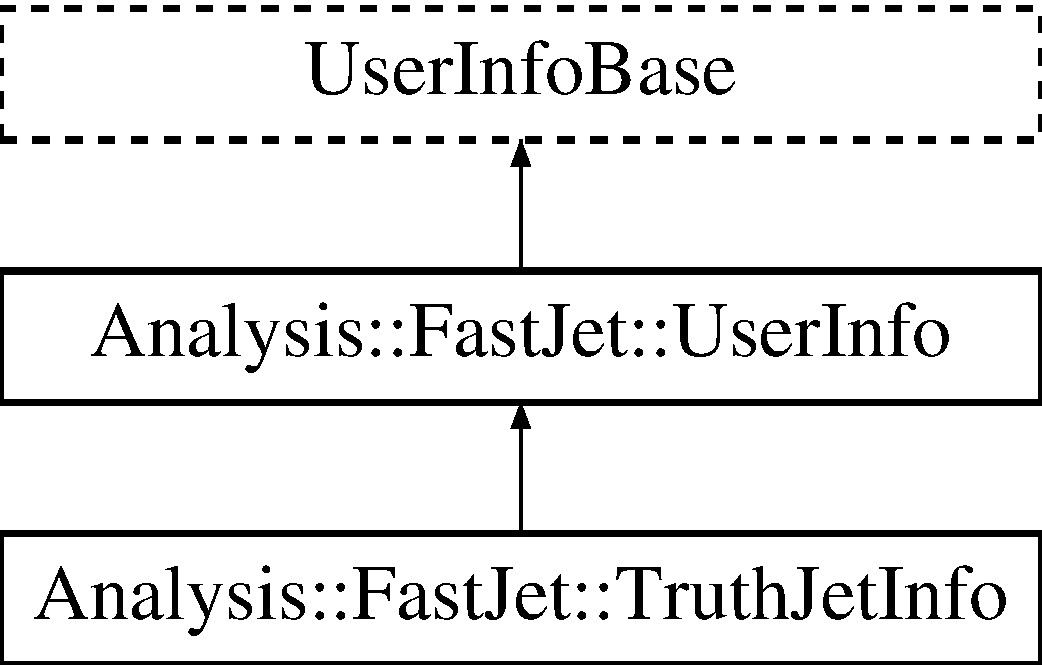
\includegraphics[height=3.000000cm]{classAnalysis_1_1FastJet_1_1TruthJetInfo}
\end{center}
\end{figure}
\subsection*{Public Member Functions}
\begin{DoxyCompactItemize}
\item 
\hyperlink{classAnalysis_1_1FastJet_1_1TruthJetInfo_ae2ae7a6f393f32397f801364dcb4bfe9}{Truth\+Jet\+Info} ()
\item 
\hyperlink{classAnalysis_1_1FastJet_1_1TruthJetInfo_ad318a0c5d02f36a24a44222980429ae9}{Truth\+Jet\+Info} (size\+\_\+t n\+Constits)
\item 
\hyperlink{classAnalysis_1_1FastJet_1_1TruthJetInfo_ae60ed5e1e6731924f3c2b30c3e9095aa}{Truth\+Jet\+Info} (const \hyperlink{classAnalysis_1_1FastJet_1_1TruthJetInfo}{Truth\+Jet\+Info} \&tjinfo)
\item 
virtual \hyperlink{classAnalysis_1_1FastJet_1_1TruthJetInfo_aaa34d97cea3e30c8c7bbc3ecdefefff1}{$\sim$\+Truth\+Jet\+Info} ()
\item 
size\+\_\+t \hyperlink{classAnalysis_1_1FastJet_1_1TruthJetInfo_a5fda799429f1c85925af4e03adaa6c09}{number\+Of\+Constituents} () const 
\item 
size\+\_\+t \hyperlink{classAnalysis_1_1FastJet_1_1TruthJetInfo_aec74be978cd1617442494c545a1cb4cb}{size} () const 
\end{DoxyCompactItemize}
\begin{Indent}{\bf Set object status}\par
{\em Set status to \char`\"{}empty\char`\"{} (no reference data) }\begin{DoxyCompactItemize}
\item 
virtual void \hyperlink{classAnalysis_1_1FastJet_1_1UserInfo_ab87ca9e42c15c24c8f54bad4b9674d0c}{set\+Empty} ()
\begin{DoxyCompactList}\small\item\em Set status to \char`\"{}faulty\char`\"{} (broken/invalid) \end{DoxyCompactList}\item 
virtual void \hyperlink{classAnalysis_1_1FastJet_1_1UserInfo_a0c5efdcfb658e75538dd5ec29c27afe0}{set\+Faulty} ()
\begin{DoxyCompactList}\small\item\em Set status to \char`\"{}faulty\char`\"{} (broken/invalid) \end{DoxyCompactList}\item 
virtual void \hyperlink{classAnalysis_1_1FastJet_1_1UserInfo_ab22ff88713e1ad12bd2311cc4f1c998c}{set\+Ghost} ()
\begin{DoxyCompactList}\small\item\em Set status to \char`\"{}ghosted\char`\"{}. \end{DoxyCompactList}\end{DoxyCompactItemize}
\end{Indent}
\begin{Indent}{\bf Access object status and data}\par
{\em Retrieve reference index (or status indicator)

\begin{DoxyReturn}{Returns}
Reference index if $>$= 0 (may still be invalid -\/ no checking); if $<$0 returns status. 
\end{DoxyReturn}
}\begin{DoxyCompactItemize}
\item 
virtual int \hyperlink{classAnalysis_1_1FastJet_1_1UserInfo_a687e6a814e58e5737108ef24aef047df}{index} () const 
\begin{DoxyCompactList}\small\item\em Check if empty. \end{DoxyCompactList}\item 
virtual bool \hyperlink{classAnalysis_1_1FastJet_1_1UserInfo_a4b987d1bba6c854cf9310596abbd3572}{is\+Empty} () const 
\begin{DoxyCompactList}\small\item\em Check if empty. \end{DoxyCompactList}\item 
virtual bool \hyperlink{classAnalysis_1_1FastJet_1_1UserInfo_a74601c143cb58b3bb62e0842b416beed}{is\+Faulty} () const 
\begin{DoxyCompactList}\small\item\em Check if faulty/broken/invalid. \end{DoxyCompactList}\item 
virtual bool \hyperlink{classAnalysis_1_1FastJet_1_1UserInfo_ad7b1ceba9d2ab04e7e7000577fe95198}{is\+Usable} () const 
\begin{DoxyCompactList}\small\item\em Check if usable. \end{DoxyCompactList}\item 
virtual bool \hyperlink{classAnalysis_1_1FastJet_1_1UserInfo_a92d2abe359ed4b794c546a23a9e1ccbe}{is\+Ghost} () const 
\begin{DoxyCompactList}\small\item\em Check if ghost. \end{DoxyCompactList}\end{DoxyCompactItemize}
\end{Indent}
\subsection*{Static Public Member Functions}
\begin{DoxyCompactItemize}
\item 
static bool \hyperlink{classAnalysis_1_1FastJet_1_1UserInfo_a79ba59c5af9a4bc2e641ab2e54e8d50b}{is\+Empty} (const fastjet\+::\+Pseudo\+Jet \&pj)
\item 
static bool \hyperlink{classAnalysis_1_1FastJet_1_1UserInfo_a18b23aae344587ff280a046e70af1d29}{is\+Usable} (const fastjet\+::\+Pseudo\+Jet \&pj)
\item 
static bool \hyperlink{classAnalysis_1_1FastJet_1_1UserInfo_a4682fdc7e258328293b05951f55cc7a1}{is\+Ghost} (const fastjet\+::\+Pseudo\+Jet \&pj)
\item 
static bool \hyperlink{classAnalysis_1_1FastJet_1_1UserInfo_a681f1076b15320ea55e7104b4fe01c3a}{has\+User\+Info} (const fastjet\+::\+Pseudo\+Jet \&pj)
\item 
static int \hyperlink{classAnalysis_1_1FastJet_1_1UserInfo_a767f93f891d045f209198cdf72fddf36}{user\+Index} (const fastjet\+::\+Pseudo\+Jet \&pj)
\end{DoxyCompactItemize}
\subsection*{Protected Attributes}
\begin{DoxyCompactItemize}
\item 
size\+\_\+t \hyperlink{classAnalysis_1_1FastJet_1_1TruthJetInfo_aba7d046daedfd7f63bcca2b85ff448aa}{\+\_\+n\+Constits}
\item 
int \hyperlink{classAnalysis_1_1FastJet_1_1UserInfo_ad9aa33e317aea2b675493b664cc718a3}{\+\_\+idx}
\begin{DoxyCompactList}\small\item\em Index to underlying structure holding data. \end{DoxyCompactList}\end{DoxyCompactItemize}


\subsection{Detailed Description}


Definition at line 479 of file Analysis\+Data.\+h.



\subsection{Constructor \& Destructor Documentation}
\index{Analysis\+::\+Fast\+Jet\+::\+Truth\+Jet\+Info@{Analysis\+::\+Fast\+Jet\+::\+Truth\+Jet\+Info}!Truth\+Jet\+Info@{Truth\+Jet\+Info}}
\index{Truth\+Jet\+Info@{Truth\+Jet\+Info}!Analysis\+::\+Fast\+Jet\+::\+Truth\+Jet\+Info@{Analysis\+::\+Fast\+Jet\+::\+Truth\+Jet\+Info}}
\subsubsection[{\texorpdfstring{Truth\+Jet\+Info()}{TruthJetInfo()}}]{\setlength{\rightskip}{0pt plus 5cm}Analysis\+::\+Fast\+Jet\+::\+Truth\+Jet\+Info\+::\+Truth\+Jet\+Info (
\begin{DoxyParamCaption}
{}
\end{DoxyParamCaption}
)\hspace{0.3cm}{\ttfamily [inline]}}\hypertarget{classAnalysis_1_1FastJet_1_1TruthJetInfo_ae2ae7a6f393f32397f801364dcb4bfe9}{}\label{classAnalysis_1_1FastJet_1_1TruthJetInfo_ae2ae7a6f393f32397f801364dcb4bfe9}


Definition at line 484 of file Analysis\+Data.\+h.

\index{Analysis\+::\+Fast\+Jet\+::\+Truth\+Jet\+Info@{Analysis\+::\+Fast\+Jet\+::\+Truth\+Jet\+Info}!Truth\+Jet\+Info@{Truth\+Jet\+Info}}
\index{Truth\+Jet\+Info@{Truth\+Jet\+Info}!Analysis\+::\+Fast\+Jet\+::\+Truth\+Jet\+Info@{Analysis\+::\+Fast\+Jet\+::\+Truth\+Jet\+Info}}
\subsubsection[{\texorpdfstring{Truth\+Jet\+Info(size\+\_\+t n\+Constits)}{TruthJetInfo(size_t nConstits)}}]{\setlength{\rightskip}{0pt plus 5cm}Analysis\+::\+Fast\+Jet\+::\+Truth\+Jet\+Info\+::\+Truth\+Jet\+Info (
\begin{DoxyParamCaption}
\item[{size\+\_\+t}]{n\+Constits}
\end{DoxyParamCaption}
)\hspace{0.3cm}{\ttfamily [inline]}}\hypertarget{classAnalysis_1_1FastJet_1_1TruthJetInfo_ad318a0c5d02f36a24a44222980429ae9}{}\label{classAnalysis_1_1FastJet_1_1TruthJetInfo_ad318a0c5d02f36a24a44222980429ae9}


Definition at line 485 of file Analysis\+Data.\+h.

\index{Analysis\+::\+Fast\+Jet\+::\+Truth\+Jet\+Info@{Analysis\+::\+Fast\+Jet\+::\+Truth\+Jet\+Info}!Truth\+Jet\+Info@{Truth\+Jet\+Info}}
\index{Truth\+Jet\+Info@{Truth\+Jet\+Info}!Analysis\+::\+Fast\+Jet\+::\+Truth\+Jet\+Info@{Analysis\+::\+Fast\+Jet\+::\+Truth\+Jet\+Info}}
\subsubsection[{\texorpdfstring{Truth\+Jet\+Info(const Truth\+Jet\+Info \&tjinfo)}{TruthJetInfo(const TruthJetInfo &tjinfo)}}]{\setlength{\rightskip}{0pt plus 5cm}Analysis\+::\+Fast\+Jet\+::\+Truth\+Jet\+Info\+::\+Truth\+Jet\+Info (
\begin{DoxyParamCaption}
\item[{const {\bf Truth\+Jet\+Info} \&}]{tjinfo}
\end{DoxyParamCaption}
)\hspace{0.3cm}{\ttfamily [inline]}}\hypertarget{classAnalysis_1_1FastJet_1_1TruthJetInfo_ae60ed5e1e6731924f3c2b30c3e9095aa}{}\label{classAnalysis_1_1FastJet_1_1TruthJetInfo_ae60ed5e1e6731924f3c2b30c3e9095aa}


Definition at line 486 of file Analysis\+Data.\+h.

\index{Analysis\+::\+Fast\+Jet\+::\+Truth\+Jet\+Info@{Analysis\+::\+Fast\+Jet\+::\+Truth\+Jet\+Info}!````~Truth\+Jet\+Info@{$\sim$\+Truth\+Jet\+Info}}
\index{````~Truth\+Jet\+Info@{$\sim$\+Truth\+Jet\+Info}!Analysis\+::\+Fast\+Jet\+::\+Truth\+Jet\+Info@{Analysis\+::\+Fast\+Jet\+::\+Truth\+Jet\+Info}}
\subsubsection[{\texorpdfstring{$\sim$\+Truth\+Jet\+Info()}{~TruthJetInfo()}}]{\setlength{\rightskip}{0pt plus 5cm}virtual Analysis\+::\+Fast\+Jet\+::\+Truth\+Jet\+Info\+::$\sim$\+Truth\+Jet\+Info (
\begin{DoxyParamCaption}
{}
\end{DoxyParamCaption}
)\hspace{0.3cm}{\ttfamily [inline]}, {\ttfamily [virtual]}}\hypertarget{classAnalysis_1_1FastJet_1_1TruthJetInfo_aaa34d97cea3e30c8c7bbc3ecdefefff1}{}\label{classAnalysis_1_1FastJet_1_1TruthJetInfo_aaa34d97cea3e30c8c7bbc3ecdefefff1}


Definition at line 487 of file Analysis\+Data.\+h.



\subsection{Member Function Documentation}
\index{Analysis\+::\+Fast\+Jet\+::\+Truth\+Jet\+Info@{Analysis\+::\+Fast\+Jet\+::\+Truth\+Jet\+Info}!has\+User\+Info@{has\+User\+Info}}
\index{has\+User\+Info@{has\+User\+Info}!Analysis\+::\+Fast\+Jet\+::\+Truth\+Jet\+Info@{Analysis\+::\+Fast\+Jet\+::\+Truth\+Jet\+Info}}
\subsubsection[{\texorpdfstring{has\+User\+Info(const fastjet\+::\+Pseudo\+Jet \&pj)}{hasUserInfo(const fastjet::PseudoJet &pj)}}]{\setlength{\rightskip}{0pt plus 5cm}static bool Analysis\+::\+Fast\+Jet\+::\+User\+Info\+::has\+User\+Info (
\begin{DoxyParamCaption}
\item[{const fastjet\+::\+Pseudo\+Jet \&}]{pj}
\end{DoxyParamCaption}
)\hspace{0.3cm}{\ttfamily [inline]}, {\ttfamily [static]}, {\ttfamily [inherited]}}\hypertarget{classAnalysis_1_1FastJet_1_1UserInfo_a681f1076b15320ea55e7104b4fe01c3a}{}\label{classAnalysis_1_1FastJet_1_1UserInfo_a681f1076b15320ea55e7104b4fe01c3a}


Definition at line 357 of file Analysis\+Data.\+h.

\index{Analysis\+::\+Fast\+Jet\+::\+Truth\+Jet\+Info@{Analysis\+::\+Fast\+Jet\+::\+Truth\+Jet\+Info}!index@{index}}
\index{index@{index}!Analysis\+::\+Fast\+Jet\+::\+Truth\+Jet\+Info@{Analysis\+::\+Fast\+Jet\+::\+Truth\+Jet\+Info}}
\subsubsection[{\texorpdfstring{index() const }{index() const }}]{\setlength{\rightskip}{0pt plus 5cm}virtual int Analysis\+::\+Fast\+Jet\+::\+User\+Info\+::index (
\begin{DoxyParamCaption}
{}
\end{DoxyParamCaption}
) const\hspace{0.3cm}{\ttfamily [inline]}, {\ttfamily [virtual]}, {\ttfamily [inherited]}}\hypertarget{classAnalysis_1_1FastJet_1_1UserInfo_a687e6a814e58e5737108ef24aef047df}{}\label{classAnalysis_1_1FastJet_1_1UserInfo_a687e6a814e58e5737108ef24aef047df}


Check if empty. 

\begin{DoxyReturn}{Returns}
{\ttfamily true} if empty. 
\end{DoxyReturn}


Definition at line 338 of file Analysis\+Data.\+h.

\index{Analysis\+::\+Fast\+Jet\+::\+Truth\+Jet\+Info@{Analysis\+::\+Fast\+Jet\+::\+Truth\+Jet\+Info}!is\+Empty@{is\+Empty}}
\index{is\+Empty@{is\+Empty}!Analysis\+::\+Fast\+Jet\+::\+Truth\+Jet\+Info@{Analysis\+::\+Fast\+Jet\+::\+Truth\+Jet\+Info}}
\subsubsection[{\texorpdfstring{is\+Empty() const }{isEmpty() const }}]{\setlength{\rightskip}{0pt plus 5cm}virtual bool Analysis\+::\+Fast\+Jet\+::\+User\+Info\+::is\+Empty (
\begin{DoxyParamCaption}
{}
\end{DoxyParamCaption}
) const\hspace{0.3cm}{\ttfamily [inline]}, {\ttfamily [virtual]}, {\ttfamily [inherited]}}\hypertarget{classAnalysis_1_1FastJet_1_1UserInfo_a4b987d1bba6c854cf9310596abbd3572}{}\label{classAnalysis_1_1FastJet_1_1UserInfo_a4b987d1bba6c854cf9310596abbd3572}


Check if empty. 

\begin{DoxyReturn}{Returns}
{\ttfamily true} if empty. 
\end{DoxyReturn}


Definition at line 342 of file Analysis\+Data.\+h.

\index{Analysis\+::\+Fast\+Jet\+::\+Truth\+Jet\+Info@{Analysis\+::\+Fast\+Jet\+::\+Truth\+Jet\+Info}!is\+Empty@{is\+Empty}}
\index{is\+Empty@{is\+Empty}!Analysis\+::\+Fast\+Jet\+::\+Truth\+Jet\+Info@{Analysis\+::\+Fast\+Jet\+::\+Truth\+Jet\+Info}}
\subsubsection[{\texorpdfstring{is\+Empty(const fastjet\+::\+Pseudo\+Jet \&pj)}{isEmpty(const fastjet::PseudoJet &pj)}}]{\setlength{\rightskip}{0pt plus 5cm}static bool Analysis\+::\+Fast\+Jet\+::\+User\+Info\+::is\+Empty (
\begin{DoxyParamCaption}
\item[{const fastjet\+::\+Pseudo\+Jet \&}]{pj}
\end{DoxyParamCaption}
)\hspace{0.3cm}{\ttfamily [inline]}, {\ttfamily [static]}, {\ttfamily [inherited]}}\hypertarget{classAnalysis_1_1FastJet_1_1UserInfo_a79ba59c5af9a4bc2e641ab2e54e8d50b}{}\label{classAnalysis_1_1FastJet_1_1UserInfo_a79ba59c5af9a4bc2e641ab2e54e8d50b}


Definition at line 362 of file Analysis\+Data.\+h.

\index{Analysis\+::\+Fast\+Jet\+::\+Truth\+Jet\+Info@{Analysis\+::\+Fast\+Jet\+::\+Truth\+Jet\+Info}!is\+Faulty@{is\+Faulty}}
\index{is\+Faulty@{is\+Faulty}!Analysis\+::\+Fast\+Jet\+::\+Truth\+Jet\+Info@{Analysis\+::\+Fast\+Jet\+::\+Truth\+Jet\+Info}}
\subsubsection[{\texorpdfstring{is\+Faulty() const }{isFaulty() const }}]{\setlength{\rightskip}{0pt plus 5cm}virtual bool Analysis\+::\+Fast\+Jet\+::\+User\+Info\+::is\+Faulty (
\begin{DoxyParamCaption}
{}
\end{DoxyParamCaption}
) const\hspace{0.3cm}{\ttfamily [inline]}, {\ttfamily [virtual]}, {\ttfamily [inherited]}}\hypertarget{classAnalysis_1_1FastJet_1_1UserInfo_a74601c143cb58b3bb62e0842b416beed}{}\label{classAnalysis_1_1FastJet_1_1UserInfo_a74601c143cb58b3bb62e0842b416beed}


Check if faulty/broken/invalid. 

\begin{DoxyReturn}{Returns}
{\ttfamily true} if faulty. 
\end{DoxyReturn}


Definition at line 346 of file Analysis\+Data.\+h.

\index{Analysis\+::\+Fast\+Jet\+::\+Truth\+Jet\+Info@{Analysis\+::\+Fast\+Jet\+::\+Truth\+Jet\+Info}!is\+Ghost@{is\+Ghost}}
\index{is\+Ghost@{is\+Ghost}!Analysis\+::\+Fast\+Jet\+::\+Truth\+Jet\+Info@{Analysis\+::\+Fast\+Jet\+::\+Truth\+Jet\+Info}}
\subsubsection[{\texorpdfstring{is\+Ghost() const }{isGhost() const }}]{\setlength{\rightskip}{0pt plus 5cm}virtual bool Analysis\+::\+Fast\+Jet\+::\+User\+Info\+::is\+Ghost (
\begin{DoxyParamCaption}
{}
\end{DoxyParamCaption}
) const\hspace{0.3cm}{\ttfamily [inline]}, {\ttfamily [virtual]}, {\ttfamily [inherited]}}\hypertarget{classAnalysis_1_1FastJet_1_1UserInfo_a92d2abe359ed4b794c546a23a9e1ccbe}{}\label{classAnalysis_1_1FastJet_1_1UserInfo_a92d2abe359ed4b794c546a23a9e1ccbe}


Check if ghost. 

\begin{DoxyReturn}{Returns}
{\ttfamily true} of associated {\ttfamily fastjet\+::\+Pseudo\+Jet} is ghosted 
\end{DoxyReturn}


Definition at line 354 of file Analysis\+Data.\+h.

\index{Analysis\+::\+Fast\+Jet\+::\+Truth\+Jet\+Info@{Analysis\+::\+Fast\+Jet\+::\+Truth\+Jet\+Info}!is\+Ghost@{is\+Ghost}}
\index{is\+Ghost@{is\+Ghost}!Analysis\+::\+Fast\+Jet\+::\+Truth\+Jet\+Info@{Analysis\+::\+Fast\+Jet\+::\+Truth\+Jet\+Info}}
\subsubsection[{\texorpdfstring{is\+Ghost(const fastjet\+::\+Pseudo\+Jet \&pj)}{isGhost(const fastjet::PseudoJet &pj)}}]{\setlength{\rightskip}{0pt plus 5cm}static bool Analysis\+::\+Fast\+Jet\+::\+User\+Info\+::is\+Ghost (
\begin{DoxyParamCaption}
\item[{const fastjet\+::\+Pseudo\+Jet \&}]{pj}
\end{DoxyParamCaption}
)\hspace{0.3cm}{\ttfamily [inline]}, {\ttfamily [static]}, {\ttfamily [inherited]}}\hypertarget{classAnalysis_1_1FastJet_1_1UserInfo_a4682fdc7e258328293b05951f55cc7a1}{}\label{classAnalysis_1_1FastJet_1_1UserInfo_a4682fdc7e258328293b05951f55cc7a1}


Definition at line 366 of file Analysis\+Data.\+h.

\index{Analysis\+::\+Fast\+Jet\+::\+Truth\+Jet\+Info@{Analysis\+::\+Fast\+Jet\+::\+Truth\+Jet\+Info}!is\+Usable@{is\+Usable}}
\index{is\+Usable@{is\+Usable}!Analysis\+::\+Fast\+Jet\+::\+Truth\+Jet\+Info@{Analysis\+::\+Fast\+Jet\+::\+Truth\+Jet\+Info}}
\subsubsection[{\texorpdfstring{is\+Usable() const }{isUsable() const }}]{\setlength{\rightskip}{0pt plus 5cm}virtual bool Analysis\+::\+Fast\+Jet\+::\+User\+Info\+::is\+Usable (
\begin{DoxyParamCaption}
{}
\end{DoxyParamCaption}
) const\hspace{0.3cm}{\ttfamily [inline]}, {\ttfamily [virtual]}, {\ttfamily [inherited]}}\hypertarget{classAnalysis_1_1FastJet_1_1UserInfo_ad7b1ceba9d2ab04e7e7000577fe95198}{}\label{classAnalysis_1_1FastJet_1_1UserInfo_ad7b1ceba9d2ab04e7e7000577fe95198}


Check if usable. 

\begin{DoxyReturn}{Returns}
{\ttfamily true} if usable -\/ no indication that the index is valid! 
\end{DoxyReturn}


Definition at line 350 of file Analysis\+Data.\+h.

\index{Analysis\+::\+Fast\+Jet\+::\+Truth\+Jet\+Info@{Analysis\+::\+Fast\+Jet\+::\+Truth\+Jet\+Info}!is\+Usable@{is\+Usable}}
\index{is\+Usable@{is\+Usable}!Analysis\+::\+Fast\+Jet\+::\+Truth\+Jet\+Info@{Analysis\+::\+Fast\+Jet\+::\+Truth\+Jet\+Info}}
\subsubsection[{\texorpdfstring{is\+Usable(const fastjet\+::\+Pseudo\+Jet \&pj)}{isUsable(const fastjet::PseudoJet &pj)}}]{\setlength{\rightskip}{0pt plus 5cm}static bool Analysis\+::\+Fast\+Jet\+::\+User\+Info\+::is\+Usable (
\begin{DoxyParamCaption}
\item[{const fastjet\+::\+Pseudo\+Jet \&}]{pj}
\end{DoxyParamCaption}
)\hspace{0.3cm}{\ttfamily [inline]}, {\ttfamily [static]}, {\ttfamily [inherited]}}\hypertarget{classAnalysis_1_1FastJet_1_1UserInfo_a18b23aae344587ff280a046e70af1d29}{}\label{classAnalysis_1_1FastJet_1_1UserInfo_a18b23aae344587ff280a046e70af1d29}


Definition at line 364 of file Analysis\+Data.\+h.

\index{Analysis\+::\+Fast\+Jet\+::\+Truth\+Jet\+Info@{Analysis\+::\+Fast\+Jet\+::\+Truth\+Jet\+Info}!number\+Of\+Constituents@{number\+Of\+Constituents}}
\index{number\+Of\+Constituents@{number\+Of\+Constituents}!Analysis\+::\+Fast\+Jet\+::\+Truth\+Jet\+Info@{Analysis\+::\+Fast\+Jet\+::\+Truth\+Jet\+Info}}
\subsubsection[{\texorpdfstring{number\+Of\+Constituents() const }{numberOfConstituents() const }}]{\setlength{\rightskip}{0pt plus 5cm}size\+\_\+t Analysis\+::\+Fast\+Jet\+::\+Truth\+Jet\+Info\+::number\+Of\+Constituents (
\begin{DoxyParamCaption}
{}
\end{DoxyParamCaption}
) const\hspace{0.3cm}{\ttfamily [inline]}}\hypertarget{classAnalysis_1_1FastJet_1_1TruthJetInfo_a5fda799429f1c85925af4e03adaa6c09}{}\label{classAnalysis_1_1FastJet_1_1TruthJetInfo_a5fda799429f1c85925af4e03adaa6c09}


Definition at line 488 of file Analysis\+Data.\+h.

\index{Analysis\+::\+Fast\+Jet\+::\+Truth\+Jet\+Info@{Analysis\+::\+Fast\+Jet\+::\+Truth\+Jet\+Info}!set\+Empty@{set\+Empty}}
\index{set\+Empty@{set\+Empty}!Analysis\+::\+Fast\+Jet\+::\+Truth\+Jet\+Info@{Analysis\+::\+Fast\+Jet\+::\+Truth\+Jet\+Info}}
\subsubsection[{\texorpdfstring{set\+Empty()}{setEmpty()}}]{\setlength{\rightskip}{0pt plus 5cm}virtual void Analysis\+::\+Fast\+Jet\+::\+User\+Info\+::set\+Empty (
\begin{DoxyParamCaption}
{}
\end{DoxyParamCaption}
)\hspace{0.3cm}{\ttfamily [inline]}, {\ttfamily [virtual]}, {\ttfamily [inherited]}}\hypertarget{classAnalysis_1_1FastJet_1_1UserInfo_ab87ca9e42c15c24c8f54bad4b9674d0c}{}\label{classAnalysis_1_1FastJet_1_1UserInfo_ab87ca9e42c15c24c8f54bad4b9674d0c}


Set status to \char`\"{}faulty\char`\"{} (broken/invalid) 



Definition at line 326 of file Analysis\+Data.\+h.

\index{Analysis\+::\+Fast\+Jet\+::\+Truth\+Jet\+Info@{Analysis\+::\+Fast\+Jet\+::\+Truth\+Jet\+Info}!set\+Faulty@{set\+Faulty}}
\index{set\+Faulty@{set\+Faulty}!Analysis\+::\+Fast\+Jet\+::\+Truth\+Jet\+Info@{Analysis\+::\+Fast\+Jet\+::\+Truth\+Jet\+Info}}
\subsubsection[{\texorpdfstring{set\+Faulty()}{setFaulty()}}]{\setlength{\rightskip}{0pt plus 5cm}virtual void Analysis\+::\+Fast\+Jet\+::\+User\+Info\+::set\+Faulty (
\begin{DoxyParamCaption}
{}
\end{DoxyParamCaption}
)\hspace{0.3cm}{\ttfamily [inline]}, {\ttfamily [virtual]}, {\ttfamily [inherited]}}\hypertarget{classAnalysis_1_1FastJet_1_1UserInfo_a0c5efdcfb658e75538dd5ec29c27afe0}{}\label{classAnalysis_1_1FastJet_1_1UserInfo_a0c5efdcfb658e75538dd5ec29c27afe0}


Set status to \char`\"{}faulty\char`\"{} (broken/invalid) 



Definition at line 328 of file Analysis\+Data.\+h.

\index{Analysis\+::\+Fast\+Jet\+::\+Truth\+Jet\+Info@{Analysis\+::\+Fast\+Jet\+::\+Truth\+Jet\+Info}!set\+Ghost@{set\+Ghost}}
\index{set\+Ghost@{set\+Ghost}!Analysis\+::\+Fast\+Jet\+::\+Truth\+Jet\+Info@{Analysis\+::\+Fast\+Jet\+::\+Truth\+Jet\+Info}}
\subsubsection[{\texorpdfstring{set\+Ghost()}{setGhost()}}]{\setlength{\rightskip}{0pt plus 5cm}virtual void Analysis\+::\+Fast\+Jet\+::\+User\+Info\+::set\+Ghost (
\begin{DoxyParamCaption}
{}
\end{DoxyParamCaption}
)\hspace{0.3cm}{\ttfamily [inline]}, {\ttfamily [virtual]}, {\ttfamily [inherited]}}\hypertarget{classAnalysis_1_1FastJet_1_1UserInfo_ab22ff88713e1ad12bd2311cc4f1c998c}{}\label{classAnalysis_1_1FastJet_1_1UserInfo_ab22ff88713e1ad12bd2311cc4f1c998c}


Set status to \char`\"{}ghosted\char`\"{}. 



Definition at line 330 of file Analysis\+Data.\+h.

\index{Analysis\+::\+Fast\+Jet\+::\+Truth\+Jet\+Info@{Analysis\+::\+Fast\+Jet\+::\+Truth\+Jet\+Info}!size@{size}}
\index{size@{size}!Analysis\+::\+Fast\+Jet\+::\+Truth\+Jet\+Info@{Analysis\+::\+Fast\+Jet\+::\+Truth\+Jet\+Info}}
\subsubsection[{\texorpdfstring{size() const }{size() const }}]{\setlength{\rightskip}{0pt plus 5cm}size\+\_\+t Analysis\+::\+Fast\+Jet\+::\+Truth\+Jet\+Info\+::size (
\begin{DoxyParamCaption}
{}
\end{DoxyParamCaption}
) const\hspace{0.3cm}{\ttfamily [inline]}}\hypertarget{classAnalysis_1_1FastJet_1_1TruthJetInfo_aec74be978cd1617442494c545a1cb4cb}{}\label{classAnalysis_1_1FastJet_1_1TruthJetInfo_aec74be978cd1617442494c545a1cb4cb}


Definition at line 489 of file Analysis\+Data.\+h.

\index{Analysis\+::\+Fast\+Jet\+::\+Truth\+Jet\+Info@{Analysis\+::\+Fast\+Jet\+::\+Truth\+Jet\+Info}!user\+Index@{user\+Index}}
\index{user\+Index@{user\+Index}!Analysis\+::\+Fast\+Jet\+::\+Truth\+Jet\+Info@{Analysis\+::\+Fast\+Jet\+::\+Truth\+Jet\+Info}}
\subsubsection[{\texorpdfstring{user\+Index(const fastjet\+::\+Pseudo\+Jet \&pj)}{userIndex(const fastjet::PseudoJet &pj)}}]{\setlength{\rightskip}{0pt plus 5cm}static int Analysis\+::\+Fast\+Jet\+::\+User\+Info\+::user\+Index (
\begin{DoxyParamCaption}
\item[{const fastjet\+::\+Pseudo\+Jet \&}]{pj}
\end{DoxyParamCaption}
)\hspace{0.3cm}{\ttfamily [inline]}, {\ttfamily [static]}, {\ttfamily [inherited]}}\hypertarget{classAnalysis_1_1FastJet_1_1UserInfo_a767f93f891d045f209198cdf72fddf36}{}\label{classAnalysis_1_1FastJet_1_1UserInfo_a767f93f891d045f209198cdf72fddf36}


Definition at line 359 of file Analysis\+Data.\+h.



\subsection{Member Data Documentation}
\index{Analysis\+::\+Fast\+Jet\+::\+Truth\+Jet\+Info@{Analysis\+::\+Fast\+Jet\+::\+Truth\+Jet\+Info}!\+\_\+idx@{\+\_\+idx}}
\index{\+\_\+idx@{\+\_\+idx}!Analysis\+::\+Fast\+Jet\+::\+Truth\+Jet\+Info@{Analysis\+::\+Fast\+Jet\+::\+Truth\+Jet\+Info}}
\subsubsection[{\texorpdfstring{\+\_\+idx}{_idx}}]{\setlength{\rightskip}{0pt plus 5cm}int Analysis\+::\+Fast\+Jet\+::\+User\+Info\+::\+\_\+idx\hspace{0.3cm}{\ttfamily [protected]}, {\ttfamily [inherited]}}\hypertarget{classAnalysis_1_1FastJet_1_1UserInfo_ad9aa33e317aea2b675493b664cc718a3}{}\label{classAnalysis_1_1FastJet_1_1UserInfo_ad9aa33e317aea2b675493b664cc718a3}


Index to underlying structure holding data. 



Definition at line 305 of file Analysis\+Data.\+h.

\index{Analysis\+::\+Fast\+Jet\+::\+Truth\+Jet\+Info@{Analysis\+::\+Fast\+Jet\+::\+Truth\+Jet\+Info}!\+\_\+n\+Constits@{\+\_\+n\+Constits}}
\index{\+\_\+n\+Constits@{\+\_\+n\+Constits}!Analysis\+::\+Fast\+Jet\+::\+Truth\+Jet\+Info@{Analysis\+::\+Fast\+Jet\+::\+Truth\+Jet\+Info}}
\subsubsection[{\texorpdfstring{\+\_\+n\+Constits}{_nConstits}}]{\setlength{\rightskip}{0pt plus 5cm}size\+\_\+t Analysis\+::\+Fast\+Jet\+::\+Truth\+Jet\+Info\+::\+\_\+n\+Constits\hspace{0.3cm}{\ttfamily [protected]}}\hypertarget{classAnalysis_1_1FastJet_1_1TruthJetInfo_aba7d046daedfd7f63bcca2b85ff448aa}{}\label{classAnalysis_1_1FastJet_1_1TruthJetInfo_aba7d046daedfd7f63bcca2b85ff448aa}


Definition at line 482 of file Analysis\+Data.\+h.



The documentation for this class was generated from the following file\+:\begin{DoxyCompactItemize}
\item 
\hyperlink{AnalysisData_8h}{Analysis\+Data.\+h}\end{DoxyCompactItemize}

\hypertarget{classAnalysis_1_1FastJet_1_1UserInfo}{}\section{Analysis\+:\+:Fast\+Jet\+:\+:User\+Info Class Reference}
\label{classAnalysis_1_1FastJet_1_1UserInfo}\index{Analysis\+::\+Fast\+Jet\+::\+User\+Info@{Analysis\+::\+Fast\+Jet\+::\+User\+Info}}


Attachment of general user information to {\ttfamily fastjet\+::\+Pseudo\+Jet}.  




{\ttfamily \#include $<$Analysis\+Data.\+h$>$}

Inheritance diagram for Analysis\+:\+:Fast\+Jet\+:\+:User\+Info\+:\begin{figure}[H]
\begin{center}
\leavevmode
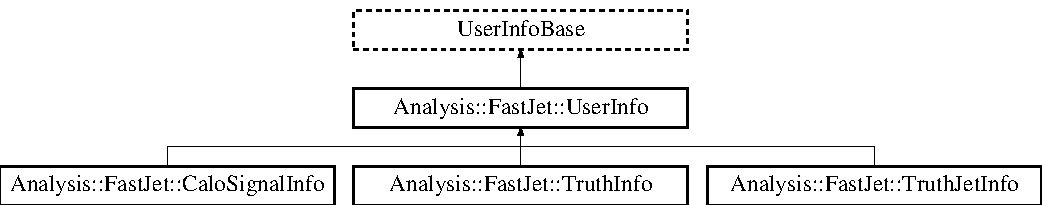
\includegraphics[height=2.758621cm]{classAnalysis_1_1FastJet_1_1UserInfo}
\end{center}
\end{figure}
\subsection*{Public Member Functions}
\begin{DoxyCompactItemize}
\item 
\hyperlink{classAnalysis_1_1FastJet_1_1UserInfo_a200d4c59fd157da608f7536449dd225b}{User\+Info} ()
\begin{DoxyCompactList}\small\item\em Default constructor. \end{DoxyCompactList}\item 
\hyperlink{classAnalysis_1_1FastJet_1_1UserInfo_af1e1e8981d308187f1722dcf6ae60039}{User\+Info} (int idx)
\begin{DoxyCompactList}\small\item\em Loaded constructor. \end{DoxyCompactList}\item 
\hyperlink{classAnalysis_1_1FastJet_1_1UserInfo_a09681790d8cfd040ee05967ceafc80f3}{User\+Info} (const \hyperlink{classAnalysis_1_1FastJet_1_1UserInfo}{User\+Info} \&ui)
\begin{DoxyCompactList}\small\item\em Copy constructor. \end{DoxyCompactList}\item 
virtual \hyperlink{classAnalysis_1_1FastJet_1_1UserInfo_aaa606bdfd9a79327258d5296fe4108a8}{$\sim$\+User\+Info} ()
\begin{DoxyCompactList}\small\item\em Destructor. \end{DoxyCompactList}\end{DoxyCompactItemize}
\begin{Indent}{\bf Set object status}\par
{\em Set status to \char`\"{}empty\char`\"{} (no reference data) }\begin{DoxyCompactItemize}
\item 
virtual void \hyperlink{classAnalysis_1_1FastJet_1_1UserInfo_ab87ca9e42c15c24c8f54bad4b9674d0c}{set\+Empty} ()
\begin{DoxyCompactList}\small\item\em Set status to \char`\"{}faulty\char`\"{} (broken/invalid) \end{DoxyCompactList}\item 
virtual void \hyperlink{classAnalysis_1_1FastJet_1_1UserInfo_a0c5efdcfb658e75538dd5ec29c27afe0}{set\+Faulty} ()
\begin{DoxyCompactList}\small\item\em Set status to \char`\"{}faulty\char`\"{} (broken/invalid) \end{DoxyCompactList}\item 
virtual void \hyperlink{classAnalysis_1_1FastJet_1_1UserInfo_ab22ff88713e1ad12bd2311cc4f1c998c}{set\+Ghost} ()
\begin{DoxyCompactList}\small\item\em Set status to \char`\"{}ghosted\char`\"{}. \end{DoxyCompactList}\end{DoxyCompactItemize}
\end{Indent}
\begin{Indent}{\bf Access object status and data}\par
{\em Retrieve reference index (or status indicator)

\begin{DoxyReturn}{Returns}
Reference index if $>$= 0 (may still be invalid -\/ no checking); if $<$0 returns status. 
\end{DoxyReturn}
}\begin{DoxyCompactItemize}
\item 
virtual int \hyperlink{classAnalysis_1_1FastJet_1_1UserInfo_a687e6a814e58e5737108ef24aef047df}{index} () const 
\begin{DoxyCompactList}\small\item\em Check if empty. \end{DoxyCompactList}\item 
virtual bool \hyperlink{classAnalysis_1_1FastJet_1_1UserInfo_a4b987d1bba6c854cf9310596abbd3572}{is\+Empty} () const 
\begin{DoxyCompactList}\small\item\em Check if empty. \end{DoxyCompactList}\item 
virtual bool \hyperlink{classAnalysis_1_1FastJet_1_1UserInfo_a74601c143cb58b3bb62e0842b416beed}{is\+Faulty} () const 
\begin{DoxyCompactList}\small\item\em Check if faulty/broken/invalid. \end{DoxyCompactList}\item 
virtual bool \hyperlink{classAnalysis_1_1FastJet_1_1UserInfo_ad7b1ceba9d2ab04e7e7000577fe95198}{is\+Usable} () const 
\begin{DoxyCompactList}\small\item\em Check if usable. \end{DoxyCompactList}\item 
virtual bool \hyperlink{classAnalysis_1_1FastJet_1_1UserInfo_a92d2abe359ed4b794c546a23a9e1ccbe}{is\+Ghost} () const 
\begin{DoxyCompactList}\small\item\em Check if ghost. \end{DoxyCompactList}\end{DoxyCompactItemize}
\end{Indent}
\subsection*{Static Public Member Functions}
\begin{DoxyCompactItemize}
\item 
static bool \hyperlink{classAnalysis_1_1FastJet_1_1UserInfo_a681f1076b15320ea55e7104b4fe01c3a}{has\+User\+Info} (const fastjet\+::\+Pseudo\+Jet \&pj)
\item 
static int \hyperlink{classAnalysis_1_1FastJet_1_1UserInfo_a767f93f891d045f209198cdf72fddf36}{user\+Index} (const fastjet\+::\+Pseudo\+Jet \&pj)
\item 
static bool \hyperlink{classAnalysis_1_1FastJet_1_1UserInfo_a79ba59c5af9a4bc2e641ab2e54e8d50b}{is\+Empty} (const fastjet\+::\+Pseudo\+Jet \&pj)
\item 
static bool \hyperlink{classAnalysis_1_1FastJet_1_1UserInfo_a18b23aae344587ff280a046e70af1d29}{is\+Usable} (const fastjet\+::\+Pseudo\+Jet \&pj)
\item 
static bool \hyperlink{classAnalysis_1_1FastJet_1_1UserInfo_a4682fdc7e258328293b05951f55cc7a1}{is\+Ghost} (const fastjet\+::\+Pseudo\+Jet \&pj)
\end{DoxyCompactItemize}
\subsection*{Protected Attributes}
\begin{DoxyCompactItemize}
\item 
int \hyperlink{classAnalysis_1_1FastJet_1_1UserInfo_ad9aa33e317aea2b675493b664cc718a3}{\+\_\+idx}
\begin{DoxyCompactList}\small\item\em Index to underlying structure holding data. \end{DoxyCompactList}\end{DoxyCompactItemize}
\subsection*{Static Private Attributes}
\begin{Indent}{\bf Status indicators}\par
\begin{DoxyCompactItemize}
\item 
static const int \hyperlink{classAnalysis_1_1FastJet_1_1UserInfo_a48e0b4a7c3bd0c598334865c7772f3d7}{\+\_\+id\+Empty} = -\/1
\begin{DoxyCompactList}\small\item\em Info object is empty. \end{DoxyCompactList}\item 
static const int \hyperlink{classAnalysis_1_1FastJet_1_1UserInfo_aadf5fa5d0ecc73ef4eacf06657cda88c}{\+\_\+id\+Broken} = -\/2
\begin{DoxyCompactList}\small\item\em Info object is broken/invalid. \end{DoxyCompactList}\item 
static const int \hyperlink{classAnalysis_1_1FastJet_1_1UserInfo_a85f8fb3a938f3a5ccffcbab501c8acbc}{\+\_\+id\+Ok} = 0
\begin{DoxyCompactList}\small\item\em Info object is ok. \end{DoxyCompactList}\item 
static const int \hyperlink{classAnalysis_1_1FastJet_1_1UserInfo_ae7eefe2914d52bb4fa38566bdb300607}{\+\_\+id\+Ghost} = -\/3
\begin{DoxyCompactList}\small\item\em Info object indicates that {\ttfamily fastjet\+::\+Pseudo\+Jet} is ghosted. \end{DoxyCompactList}\end{DoxyCompactItemize}
\end{Indent}


\subsection{Detailed Description}
Attachment of general user information to {\ttfamily fastjet\+::\+Pseudo\+Jet}. 

This object provides a store for an index which in previous implementations was intended to reference the index of the data in the underlying data structure (e.\+g. a {\ttfamily R\+O\+OT} tuple). This index can in general not be relied on since the \char`\"{}ghosted\char`\"{} status is now available. A ghosted {\ttfamily fastjet\+::\+Pseudo\+Jet} can have a valid reference index, but will return a numerical value $<$ 0 when using the {\ttfamily \hyperlink{classAnalysis_1_1FastJet_1_1UserInfo_a687e6a814e58e5737108ef24aef047df}{index()}} function. Therefore this function should not be used if possible. Rather, the index to the underlyging data structure is now available directly using the {\ttfamily fastjet\+::\+Pseudo\+Jet\+::user\+\_\+index()} feature.

\begin{DoxyRefDesc}{Todo}
\item[\hyperlink{todo__todo000001}{Todo}]Fix the index/status handling to a more obvious behaviour. \end{DoxyRefDesc}


Definition at line 293 of file Analysis\+Data.\+h.



\subsection{Constructor \& Destructor Documentation}
\index{Analysis\+::\+Fast\+Jet\+::\+User\+Info@{Analysis\+::\+Fast\+Jet\+::\+User\+Info}!User\+Info@{User\+Info}}
\index{User\+Info@{User\+Info}!Analysis\+::\+Fast\+Jet\+::\+User\+Info@{Analysis\+::\+Fast\+Jet\+::\+User\+Info}}
\subsubsection[{\texorpdfstring{User\+Info()}{UserInfo()}}]{\setlength{\rightskip}{0pt plus 5cm}Analysis\+::\+Fast\+Jet\+::\+User\+Info\+::\+User\+Info (
\begin{DoxyParamCaption}
{}
\end{DoxyParamCaption}
)\hspace{0.3cm}{\ttfamily [inline]}}\hypertarget{classAnalysis_1_1FastJet_1_1UserInfo_a200d4c59fd157da608f7536449dd225b}{}\label{classAnalysis_1_1FastJet_1_1UserInfo_a200d4c59fd157da608f7536449dd225b}


Default constructor. 

Instantiates an empty {\ttfamily \hyperlink{classAnalysis_1_1FastJet_1_1UserInfo}{User\+Info}} object 

Definition at line 310 of file Analysis\+Data.\+h.

\index{Analysis\+::\+Fast\+Jet\+::\+User\+Info@{Analysis\+::\+Fast\+Jet\+::\+User\+Info}!User\+Info@{User\+Info}}
\index{User\+Info@{User\+Info}!Analysis\+::\+Fast\+Jet\+::\+User\+Info@{Analysis\+::\+Fast\+Jet\+::\+User\+Info}}
\subsubsection[{\texorpdfstring{User\+Info(int idx)}{UserInfo(int idx)}}]{\setlength{\rightskip}{0pt plus 5cm}Analysis\+::\+Fast\+Jet\+::\+User\+Info\+::\+User\+Info (
\begin{DoxyParamCaption}
\item[{int}]{idx}
\end{DoxyParamCaption}
)\hspace{0.3cm}{\ttfamily [inline]}}\hypertarget{classAnalysis_1_1FastJet_1_1UserInfo_af1e1e8981d308187f1722dcf6ae60039}{}\label{classAnalysis_1_1FastJet_1_1UserInfo_af1e1e8981d308187f1722dcf6ae60039}


Loaded constructor. 

Instantiates a {\ttfamily \hyperlink{classAnalysis_1_1FastJet_1_1UserInfo}{User\+Info}} object with a reference index. There is no check on the validity of this index. 
\begin{DoxyParams}{Parameters}
{\em idx} & reference index \\
\hline
\end{DoxyParams}


Definition at line 315 of file Analysis\+Data.\+h.

\index{Analysis\+::\+Fast\+Jet\+::\+User\+Info@{Analysis\+::\+Fast\+Jet\+::\+User\+Info}!User\+Info@{User\+Info}}
\index{User\+Info@{User\+Info}!Analysis\+::\+Fast\+Jet\+::\+User\+Info@{Analysis\+::\+Fast\+Jet\+::\+User\+Info}}
\subsubsection[{\texorpdfstring{User\+Info(const User\+Info \&ui)}{UserInfo(const UserInfo &ui)}}]{\setlength{\rightskip}{0pt plus 5cm}Analysis\+::\+Fast\+Jet\+::\+User\+Info\+::\+User\+Info (
\begin{DoxyParamCaption}
\item[{const {\bf User\+Info} \&}]{ui}
\end{DoxyParamCaption}
)\hspace{0.3cm}{\ttfamily [inline]}}\hypertarget{classAnalysis_1_1FastJet_1_1UserInfo_a09681790d8cfd040ee05967ceafc80f3}{}\label{classAnalysis_1_1FastJet_1_1UserInfo_a09681790d8cfd040ee05967ceafc80f3}


Copy constructor. 



Definition at line 317 of file Analysis\+Data.\+h.

\index{Analysis\+::\+Fast\+Jet\+::\+User\+Info@{Analysis\+::\+Fast\+Jet\+::\+User\+Info}!````~User\+Info@{$\sim$\+User\+Info}}
\index{````~User\+Info@{$\sim$\+User\+Info}!Analysis\+::\+Fast\+Jet\+::\+User\+Info@{Analysis\+::\+Fast\+Jet\+::\+User\+Info}}
\subsubsection[{\texorpdfstring{$\sim$\+User\+Info()}{~UserInfo()}}]{\setlength{\rightskip}{0pt plus 5cm}virtual Analysis\+::\+Fast\+Jet\+::\+User\+Info\+::$\sim$\+User\+Info (
\begin{DoxyParamCaption}
{}
\end{DoxyParamCaption}
)\hspace{0.3cm}{\ttfamily [inline]}, {\ttfamily [virtual]}}\hypertarget{classAnalysis_1_1FastJet_1_1UserInfo_aaa606bdfd9a79327258d5296fe4108a8}{}\label{classAnalysis_1_1FastJet_1_1UserInfo_aaa606bdfd9a79327258d5296fe4108a8}


Destructor. 



Definition at line 321 of file Analysis\+Data.\+h.



\subsection{Member Function Documentation}
\index{Analysis\+::\+Fast\+Jet\+::\+User\+Info@{Analysis\+::\+Fast\+Jet\+::\+User\+Info}!has\+User\+Info@{has\+User\+Info}}
\index{has\+User\+Info@{has\+User\+Info}!Analysis\+::\+Fast\+Jet\+::\+User\+Info@{Analysis\+::\+Fast\+Jet\+::\+User\+Info}}
\subsubsection[{\texorpdfstring{has\+User\+Info(const fastjet\+::\+Pseudo\+Jet \&pj)}{hasUserInfo(const fastjet::PseudoJet &pj)}}]{\setlength{\rightskip}{0pt plus 5cm}static bool Analysis\+::\+Fast\+Jet\+::\+User\+Info\+::has\+User\+Info (
\begin{DoxyParamCaption}
\item[{const fastjet\+::\+Pseudo\+Jet \&}]{pj}
\end{DoxyParamCaption}
)\hspace{0.3cm}{\ttfamily [inline]}, {\ttfamily [static]}}\hypertarget{classAnalysis_1_1FastJet_1_1UserInfo_a681f1076b15320ea55e7104b4fe01c3a}{}\label{classAnalysis_1_1FastJet_1_1UserInfo_a681f1076b15320ea55e7104b4fe01c3a}


Definition at line 357 of file Analysis\+Data.\+h.

\index{Analysis\+::\+Fast\+Jet\+::\+User\+Info@{Analysis\+::\+Fast\+Jet\+::\+User\+Info}!index@{index}}
\index{index@{index}!Analysis\+::\+Fast\+Jet\+::\+User\+Info@{Analysis\+::\+Fast\+Jet\+::\+User\+Info}}
\subsubsection[{\texorpdfstring{index() const }{index() const }}]{\setlength{\rightskip}{0pt plus 5cm}virtual int Analysis\+::\+Fast\+Jet\+::\+User\+Info\+::index (
\begin{DoxyParamCaption}
{}
\end{DoxyParamCaption}
) const\hspace{0.3cm}{\ttfamily [inline]}, {\ttfamily [virtual]}}\hypertarget{classAnalysis_1_1FastJet_1_1UserInfo_a687e6a814e58e5737108ef24aef047df}{}\label{classAnalysis_1_1FastJet_1_1UserInfo_a687e6a814e58e5737108ef24aef047df}


Check if empty. 

\begin{DoxyReturn}{Returns}
{\ttfamily true} if empty. 
\end{DoxyReturn}


Definition at line 338 of file Analysis\+Data.\+h.

\index{Analysis\+::\+Fast\+Jet\+::\+User\+Info@{Analysis\+::\+Fast\+Jet\+::\+User\+Info}!is\+Empty@{is\+Empty}}
\index{is\+Empty@{is\+Empty}!Analysis\+::\+Fast\+Jet\+::\+User\+Info@{Analysis\+::\+Fast\+Jet\+::\+User\+Info}}
\subsubsection[{\texorpdfstring{is\+Empty() const }{isEmpty() const }}]{\setlength{\rightskip}{0pt plus 5cm}virtual bool Analysis\+::\+Fast\+Jet\+::\+User\+Info\+::is\+Empty (
\begin{DoxyParamCaption}
{}
\end{DoxyParamCaption}
) const\hspace{0.3cm}{\ttfamily [inline]}, {\ttfamily [virtual]}}\hypertarget{classAnalysis_1_1FastJet_1_1UserInfo_a4b987d1bba6c854cf9310596abbd3572}{}\label{classAnalysis_1_1FastJet_1_1UserInfo_a4b987d1bba6c854cf9310596abbd3572}


Check if empty. 

\begin{DoxyReturn}{Returns}
{\ttfamily true} if empty. 
\end{DoxyReturn}


Definition at line 342 of file Analysis\+Data.\+h.

\index{Analysis\+::\+Fast\+Jet\+::\+User\+Info@{Analysis\+::\+Fast\+Jet\+::\+User\+Info}!is\+Empty@{is\+Empty}}
\index{is\+Empty@{is\+Empty}!Analysis\+::\+Fast\+Jet\+::\+User\+Info@{Analysis\+::\+Fast\+Jet\+::\+User\+Info}}
\subsubsection[{\texorpdfstring{is\+Empty(const fastjet\+::\+Pseudo\+Jet \&pj)}{isEmpty(const fastjet::PseudoJet &pj)}}]{\setlength{\rightskip}{0pt plus 5cm}static bool Analysis\+::\+Fast\+Jet\+::\+User\+Info\+::is\+Empty (
\begin{DoxyParamCaption}
\item[{const fastjet\+::\+Pseudo\+Jet \&}]{pj}
\end{DoxyParamCaption}
)\hspace{0.3cm}{\ttfamily [inline]}, {\ttfamily [static]}}\hypertarget{classAnalysis_1_1FastJet_1_1UserInfo_a79ba59c5af9a4bc2e641ab2e54e8d50b}{}\label{classAnalysis_1_1FastJet_1_1UserInfo_a79ba59c5af9a4bc2e641ab2e54e8d50b}


Definition at line 362 of file Analysis\+Data.\+h.

\index{Analysis\+::\+Fast\+Jet\+::\+User\+Info@{Analysis\+::\+Fast\+Jet\+::\+User\+Info}!is\+Faulty@{is\+Faulty}}
\index{is\+Faulty@{is\+Faulty}!Analysis\+::\+Fast\+Jet\+::\+User\+Info@{Analysis\+::\+Fast\+Jet\+::\+User\+Info}}
\subsubsection[{\texorpdfstring{is\+Faulty() const }{isFaulty() const }}]{\setlength{\rightskip}{0pt plus 5cm}virtual bool Analysis\+::\+Fast\+Jet\+::\+User\+Info\+::is\+Faulty (
\begin{DoxyParamCaption}
{}
\end{DoxyParamCaption}
) const\hspace{0.3cm}{\ttfamily [inline]}, {\ttfamily [virtual]}}\hypertarget{classAnalysis_1_1FastJet_1_1UserInfo_a74601c143cb58b3bb62e0842b416beed}{}\label{classAnalysis_1_1FastJet_1_1UserInfo_a74601c143cb58b3bb62e0842b416beed}


Check if faulty/broken/invalid. 

\begin{DoxyReturn}{Returns}
{\ttfamily true} if faulty. 
\end{DoxyReturn}


Definition at line 346 of file Analysis\+Data.\+h.

\index{Analysis\+::\+Fast\+Jet\+::\+User\+Info@{Analysis\+::\+Fast\+Jet\+::\+User\+Info}!is\+Ghost@{is\+Ghost}}
\index{is\+Ghost@{is\+Ghost}!Analysis\+::\+Fast\+Jet\+::\+User\+Info@{Analysis\+::\+Fast\+Jet\+::\+User\+Info}}
\subsubsection[{\texorpdfstring{is\+Ghost() const }{isGhost() const }}]{\setlength{\rightskip}{0pt plus 5cm}virtual bool Analysis\+::\+Fast\+Jet\+::\+User\+Info\+::is\+Ghost (
\begin{DoxyParamCaption}
{}
\end{DoxyParamCaption}
) const\hspace{0.3cm}{\ttfamily [inline]}, {\ttfamily [virtual]}}\hypertarget{classAnalysis_1_1FastJet_1_1UserInfo_a92d2abe359ed4b794c546a23a9e1ccbe}{}\label{classAnalysis_1_1FastJet_1_1UserInfo_a92d2abe359ed4b794c546a23a9e1ccbe}


Check if ghost. 

\begin{DoxyReturn}{Returns}
{\ttfamily true} of associated {\ttfamily fastjet\+::\+Pseudo\+Jet} is ghosted 
\end{DoxyReturn}


Definition at line 354 of file Analysis\+Data.\+h.

\index{Analysis\+::\+Fast\+Jet\+::\+User\+Info@{Analysis\+::\+Fast\+Jet\+::\+User\+Info}!is\+Ghost@{is\+Ghost}}
\index{is\+Ghost@{is\+Ghost}!Analysis\+::\+Fast\+Jet\+::\+User\+Info@{Analysis\+::\+Fast\+Jet\+::\+User\+Info}}
\subsubsection[{\texorpdfstring{is\+Ghost(const fastjet\+::\+Pseudo\+Jet \&pj)}{isGhost(const fastjet::PseudoJet &pj)}}]{\setlength{\rightskip}{0pt plus 5cm}static bool Analysis\+::\+Fast\+Jet\+::\+User\+Info\+::is\+Ghost (
\begin{DoxyParamCaption}
\item[{const fastjet\+::\+Pseudo\+Jet \&}]{pj}
\end{DoxyParamCaption}
)\hspace{0.3cm}{\ttfamily [inline]}, {\ttfamily [static]}}\hypertarget{classAnalysis_1_1FastJet_1_1UserInfo_a4682fdc7e258328293b05951f55cc7a1}{}\label{classAnalysis_1_1FastJet_1_1UserInfo_a4682fdc7e258328293b05951f55cc7a1}


Definition at line 366 of file Analysis\+Data.\+h.

\index{Analysis\+::\+Fast\+Jet\+::\+User\+Info@{Analysis\+::\+Fast\+Jet\+::\+User\+Info}!is\+Usable@{is\+Usable}}
\index{is\+Usable@{is\+Usable}!Analysis\+::\+Fast\+Jet\+::\+User\+Info@{Analysis\+::\+Fast\+Jet\+::\+User\+Info}}
\subsubsection[{\texorpdfstring{is\+Usable() const }{isUsable() const }}]{\setlength{\rightskip}{0pt plus 5cm}virtual bool Analysis\+::\+Fast\+Jet\+::\+User\+Info\+::is\+Usable (
\begin{DoxyParamCaption}
{}
\end{DoxyParamCaption}
) const\hspace{0.3cm}{\ttfamily [inline]}, {\ttfamily [virtual]}}\hypertarget{classAnalysis_1_1FastJet_1_1UserInfo_ad7b1ceba9d2ab04e7e7000577fe95198}{}\label{classAnalysis_1_1FastJet_1_1UserInfo_ad7b1ceba9d2ab04e7e7000577fe95198}


Check if usable. 

\begin{DoxyReturn}{Returns}
{\ttfamily true} if usable -\/ no indication that the index is valid! 
\end{DoxyReturn}


Definition at line 350 of file Analysis\+Data.\+h.

\index{Analysis\+::\+Fast\+Jet\+::\+User\+Info@{Analysis\+::\+Fast\+Jet\+::\+User\+Info}!is\+Usable@{is\+Usable}}
\index{is\+Usable@{is\+Usable}!Analysis\+::\+Fast\+Jet\+::\+User\+Info@{Analysis\+::\+Fast\+Jet\+::\+User\+Info}}
\subsubsection[{\texorpdfstring{is\+Usable(const fastjet\+::\+Pseudo\+Jet \&pj)}{isUsable(const fastjet::PseudoJet &pj)}}]{\setlength{\rightskip}{0pt plus 5cm}static bool Analysis\+::\+Fast\+Jet\+::\+User\+Info\+::is\+Usable (
\begin{DoxyParamCaption}
\item[{const fastjet\+::\+Pseudo\+Jet \&}]{pj}
\end{DoxyParamCaption}
)\hspace{0.3cm}{\ttfamily [inline]}, {\ttfamily [static]}}\hypertarget{classAnalysis_1_1FastJet_1_1UserInfo_a18b23aae344587ff280a046e70af1d29}{}\label{classAnalysis_1_1FastJet_1_1UserInfo_a18b23aae344587ff280a046e70af1d29}


Definition at line 364 of file Analysis\+Data.\+h.

\index{Analysis\+::\+Fast\+Jet\+::\+User\+Info@{Analysis\+::\+Fast\+Jet\+::\+User\+Info}!set\+Empty@{set\+Empty}}
\index{set\+Empty@{set\+Empty}!Analysis\+::\+Fast\+Jet\+::\+User\+Info@{Analysis\+::\+Fast\+Jet\+::\+User\+Info}}
\subsubsection[{\texorpdfstring{set\+Empty()}{setEmpty()}}]{\setlength{\rightskip}{0pt plus 5cm}virtual void Analysis\+::\+Fast\+Jet\+::\+User\+Info\+::set\+Empty (
\begin{DoxyParamCaption}
{}
\end{DoxyParamCaption}
)\hspace{0.3cm}{\ttfamily [inline]}, {\ttfamily [virtual]}}\hypertarget{classAnalysis_1_1FastJet_1_1UserInfo_ab87ca9e42c15c24c8f54bad4b9674d0c}{}\label{classAnalysis_1_1FastJet_1_1UserInfo_ab87ca9e42c15c24c8f54bad4b9674d0c}


Set status to \char`\"{}faulty\char`\"{} (broken/invalid) 



Definition at line 326 of file Analysis\+Data.\+h.

\index{Analysis\+::\+Fast\+Jet\+::\+User\+Info@{Analysis\+::\+Fast\+Jet\+::\+User\+Info}!set\+Faulty@{set\+Faulty}}
\index{set\+Faulty@{set\+Faulty}!Analysis\+::\+Fast\+Jet\+::\+User\+Info@{Analysis\+::\+Fast\+Jet\+::\+User\+Info}}
\subsubsection[{\texorpdfstring{set\+Faulty()}{setFaulty()}}]{\setlength{\rightskip}{0pt plus 5cm}virtual void Analysis\+::\+Fast\+Jet\+::\+User\+Info\+::set\+Faulty (
\begin{DoxyParamCaption}
{}
\end{DoxyParamCaption}
)\hspace{0.3cm}{\ttfamily [inline]}, {\ttfamily [virtual]}}\hypertarget{classAnalysis_1_1FastJet_1_1UserInfo_a0c5efdcfb658e75538dd5ec29c27afe0}{}\label{classAnalysis_1_1FastJet_1_1UserInfo_a0c5efdcfb658e75538dd5ec29c27afe0}


Set status to \char`\"{}faulty\char`\"{} (broken/invalid) 



Definition at line 328 of file Analysis\+Data.\+h.

\index{Analysis\+::\+Fast\+Jet\+::\+User\+Info@{Analysis\+::\+Fast\+Jet\+::\+User\+Info}!set\+Ghost@{set\+Ghost}}
\index{set\+Ghost@{set\+Ghost}!Analysis\+::\+Fast\+Jet\+::\+User\+Info@{Analysis\+::\+Fast\+Jet\+::\+User\+Info}}
\subsubsection[{\texorpdfstring{set\+Ghost()}{setGhost()}}]{\setlength{\rightskip}{0pt plus 5cm}virtual void Analysis\+::\+Fast\+Jet\+::\+User\+Info\+::set\+Ghost (
\begin{DoxyParamCaption}
{}
\end{DoxyParamCaption}
)\hspace{0.3cm}{\ttfamily [inline]}, {\ttfamily [virtual]}}\hypertarget{classAnalysis_1_1FastJet_1_1UserInfo_ab22ff88713e1ad12bd2311cc4f1c998c}{}\label{classAnalysis_1_1FastJet_1_1UserInfo_ab22ff88713e1ad12bd2311cc4f1c998c}


Set status to \char`\"{}ghosted\char`\"{}. 



Definition at line 330 of file Analysis\+Data.\+h.

\index{Analysis\+::\+Fast\+Jet\+::\+User\+Info@{Analysis\+::\+Fast\+Jet\+::\+User\+Info}!user\+Index@{user\+Index}}
\index{user\+Index@{user\+Index}!Analysis\+::\+Fast\+Jet\+::\+User\+Info@{Analysis\+::\+Fast\+Jet\+::\+User\+Info}}
\subsubsection[{\texorpdfstring{user\+Index(const fastjet\+::\+Pseudo\+Jet \&pj)}{userIndex(const fastjet::PseudoJet &pj)}}]{\setlength{\rightskip}{0pt plus 5cm}static int Analysis\+::\+Fast\+Jet\+::\+User\+Info\+::user\+Index (
\begin{DoxyParamCaption}
\item[{const fastjet\+::\+Pseudo\+Jet \&}]{pj}
\end{DoxyParamCaption}
)\hspace{0.3cm}{\ttfamily [inline]}, {\ttfamily [static]}}\hypertarget{classAnalysis_1_1FastJet_1_1UserInfo_a767f93f891d045f209198cdf72fddf36}{}\label{classAnalysis_1_1FastJet_1_1UserInfo_a767f93f891d045f209198cdf72fddf36}


Definition at line 359 of file Analysis\+Data.\+h.



\subsection{Member Data Documentation}
\index{Analysis\+::\+Fast\+Jet\+::\+User\+Info@{Analysis\+::\+Fast\+Jet\+::\+User\+Info}!\+\_\+id\+Broken@{\+\_\+id\+Broken}}
\index{\+\_\+id\+Broken@{\+\_\+id\+Broken}!Analysis\+::\+Fast\+Jet\+::\+User\+Info@{Analysis\+::\+Fast\+Jet\+::\+User\+Info}}
\subsubsection[{\texorpdfstring{\+\_\+id\+Broken}{_idBroken}}]{\setlength{\rightskip}{0pt plus 5cm}const int Analysis\+::\+Fast\+Jet\+::\+User\+Info\+::\+\_\+id\+Broken = -\/2\hspace{0.3cm}{\ttfamily [static]}, {\ttfamily [private]}}\hypertarget{classAnalysis_1_1FastJet_1_1UserInfo_aadf5fa5d0ecc73ef4eacf06657cda88c}{}\label{classAnalysis_1_1FastJet_1_1UserInfo_aadf5fa5d0ecc73ef4eacf06657cda88c}


Info object is broken/invalid. 



Definition at line 299 of file Analysis\+Data.\+h.

\index{Analysis\+::\+Fast\+Jet\+::\+User\+Info@{Analysis\+::\+Fast\+Jet\+::\+User\+Info}!\+\_\+id\+Empty@{\+\_\+id\+Empty}}
\index{\+\_\+id\+Empty@{\+\_\+id\+Empty}!Analysis\+::\+Fast\+Jet\+::\+User\+Info@{Analysis\+::\+Fast\+Jet\+::\+User\+Info}}
\subsubsection[{\texorpdfstring{\+\_\+id\+Empty}{_idEmpty}}]{\setlength{\rightskip}{0pt plus 5cm}const int Analysis\+::\+Fast\+Jet\+::\+User\+Info\+::\+\_\+id\+Empty = -\/1\hspace{0.3cm}{\ttfamily [static]}, {\ttfamily [private]}}\hypertarget{classAnalysis_1_1FastJet_1_1UserInfo_a48e0b4a7c3bd0c598334865c7772f3d7}{}\label{classAnalysis_1_1FastJet_1_1UserInfo_a48e0b4a7c3bd0c598334865c7772f3d7}


Info object is empty. 



Definition at line 298 of file Analysis\+Data.\+h.

\index{Analysis\+::\+Fast\+Jet\+::\+User\+Info@{Analysis\+::\+Fast\+Jet\+::\+User\+Info}!\+\_\+id\+Ghost@{\+\_\+id\+Ghost}}
\index{\+\_\+id\+Ghost@{\+\_\+id\+Ghost}!Analysis\+::\+Fast\+Jet\+::\+User\+Info@{Analysis\+::\+Fast\+Jet\+::\+User\+Info}}
\subsubsection[{\texorpdfstring{\+\_\+id\+Ghost}{_idGhost}}]{\setlength{\rightskip}{0pt plus 5cm}const int Analysis\+::\+Fast\+Jet\+::\+User\+Info\+::\+\_\+id\+Ghost = -\/3\hspace{0.3cm}{\ttfamily [static]}, {\ttfamily [private]}}\hypertarget{classAnalysis_1_1FastJet_1_1UserInfo_ae7eefe2914d52bb4fa38566bdb300607}{}\label{classAnalysis_1_1FastJet_1_1UserInfo_ae7eefe2914d52bb4fa38566bdb300607}


Info object indicates that {\ttfamily fastjet\+::\+Pseudo\+Jet} is ghosted. 



Definition at line 301 of file Analysis\+Data.\+h.

\index{Analysis\+::\+Fast\+Jet\+::\+User\+Info@{Analysis\+::\+Fast\+Jet\+::\+User\+Info}!\+\_\+id\+Ok@{\+\_\+id\+Ok}}
\index{\+\_\+id\+Ok@{\+\_\+id\+Ok}!Analysis\+::\+Fast\+Jet\+::\+User\+Info@{Analysis\+::\+Fast\+Jet\+::\+User\+Info}}
\subsubsection[{\texorpdfstring{\+\_\+id\+Ok}{_idOk}}]{\setlength{\rightskip}{0pt plus 5cm}const int Analysis\+::\+Fast\+Jet\+::\+User\+Info\+::\+\_\+id\+Ok = 0\hspace{0.3cm}{\ttfamily [static]}, {\ttfamily [private]}}\hypertarget{classAnalysis_1_1FastJet_1_1UserInfo_a85f8fb3a938f3a5ccffcbab501c8acbc}{}\label{classAnalysis_1_1FastJet_1_1UserInfo_a85f8fb3a938f3a5ccffcbab501c8acbc}


Info object is ok. 



Definition at line 300 of file Analysis\+Data.\+h.

\index{Analysis\+::\+Fast\+Jet\+::\+User\+Info@{Analysis\+::\+Fast\+Jet\+::\+User\+Info}!\+\_\+idx@{\+\_\+idx}}
\index{\+\_\+idx@{\+\_\+idx}!Analysis\+::\+Fast\+Jet\+::\+User\+Info@{Analysis\+::\+Fast\+Jet\+::\+User\+Info}}
\subsubsection[{\texorpdfstring{\+\_\+idx}{_idx}}]{\setlength{\rightskip}{0pt plus 5cm}int Analysis\+::\+Fast\+Jet\+::\+User\+Info\+::\+\_\+idx\hspace{0.3cm}{\ttfamily [protected]}}\hypertarget{classAnalysis_1_1FastJet_1_1UserInfo_ad9aa33e317aea2b675493b664cc718a3}{}\label{classAnalysis_1_1FastJet_1_1UserInfo_ad9aa33e317aea2b675493b664cc718a3}


Index to underlying structure holding data. 



Definition at line 305 of file Analysis\+Data.\+h.



The documentation for this class was generated from the following file\+:\begin{DoxyCompactItemize}
\item 
\hyperlink{AnalysisData_8h}{Analysis\+Data.\+h}\end{DoxyCompactItemize}

\hypertarget{classSlidingWindow_1_1Window}{}\section{Sliding\+Window\+:\+:Window Class Reference}
\label{classSlidingWindow_1_1Window}\index{Sliding\+Window\+::\+Window@{Sliding\+Window\+::\+Window}}


\hyperlink{classSlidingWindow_1_1Window}{Window} collector.  




{\ttfamily \#include $<$Sliding\+Window.\+h$>$}

\subsection*{Classes}
\begin{DoxyCompactItemize}
\item 
struct \hyperlink{structSlidingWindow_1_1Window_1_1__sortObjects}{\+\_\+sort\+Objects}
\end{DoxyCompactItemize}
\subsection*{Public Types}
\begin{Indent}{\bf Data types}\par
\begin{DoxyCompactItemize}
\item 
typedef std\+::vector$<$ double $>$ \hyperlink{classSlidingWindow_1_1Window_abc07b028eea17a8713e74a556b9d1ad2}{data\+\_\+t}
\begin{DoxyCompactList}\small\item\em Real number list type. \end{DoxyCompactList}\item 
typedef std\+::vector$<$ \hyperlink{classSlidingWindow_1_1Window_abc07b028eea17a8713e74a556b9d1ad2}{data\+\_\+t} $>$ \hyperlink{classSlidingWindow_1_1Window_a86da88957da29f042341ff4b0413316e}{collector\+\_\+t}
\begin{DoxyCompactList}\small\item\em Real number matrix type (2-\/dimensional) \end{DoxyCompactList}\item 
typedef std\+::vector$<$ fastjet\+::\+Pseudo\+Jet $>$ \hyperlink{classSlidingWindow_1_1Window_a0ee13c18faf2f2ec3855b6449ef765e0}{object\+\_\+t}
\begin{DoxyCompactList}\small\item\em Object list type. \end{DoxyCompactList}\item 
typedef std\+::vector$<$ \hyperlink{classSlidingWindow_1_1Window_a0ee13c18faf2f2ec3855b6449ef765e0}{object\+\_\+t} $>$ \hyperlink{classSlidingWindow_1_1Window_a3883a474287703a42cf8971ba8ef6884}{object\+\_\+collector\+\_\+t}
\begin{DoxyCompactList}\small\item\em Object matrix type (2-\/dimensional) \end{DoxyCompactList}\item 
typedef \hyperlink{classSlidingWindow_1_1Bin}{Bin} \hyperlink{classSlidingWindow_1_1Window_a9bbfc142a52e17a3e1c51093edfe936f}{bin\+\_\+t}
\begin{DoxyCompactList}\small\item\em \hyperlink{classSlidingWindow_1_1Bin}{Bin} descriptor type. \end{DoxyCompactList}\item 
typedef std\+::vector$<$ \hyperlink{classSlidingWindow_1_1Window_a9bbfc142a52e17a3e1c51093edfe936f}{bin\+\_\+t} $>$ \hyperlink{classSlidingWindow_1_1Window_a71c711c04a16a1f32a9731f80e73b5e8}{binning\+\_\+t}
\begin{DoxyCompactList}\small\item\em List of bin descriptors type. \end{DoxyCompactList}\end{DoxyCompactItemize}
\end{Indent}
\subsection*{Public Member Functions}
\begin{DoxyCompactItemize}
\item 
\hyperlink{classSlidingWindow_1_1Window_adaccac4f0906832d5417de50a82fb068}{Window} ()
\begin{DoxyCompactList}\small\item\em Default constructor. \end{DoxyCompactList}\item 
\hyperlink{classSlidingWindow_1_1Window_a4e940851f8491269fa36c267a94713c0}{Window} (const std\+::string \&p\+Name, size\+\_\+t n\+Bins, double \hyperlink{classSlidingWindow_1_1Window_a9f134cb80a395f11025c5d0fa1465852}{min}, double \hyperlink{classSlidingWindow_1_1Window_a57ad1e073130318a845129c8d92dae4c}{max}, double window, bool store\+Objects=false)
\begin{DoxyCompactList}\small\item\em Loaded constructor. \end{DoxyCompactList}\item 
virtual \hyperlink{classSlidingWindow_1_1Window_aeacafc20517bb5509871450e75151fca}{$\sim$\+Window} ()
\begin{DoxyCompactList}\small\item\em Base class destructor. \end{DoxyCompactList}\end{DoxyCompactItemize}
\begin{Indent}{\bf Configurations and states}\par
{\em Book sliding window collector


\begin{DoxyParams}{Parameters}
{\em prn} & controls printout; if {\ttfamily true} (default) details of the collector configuration are printed, else printing is suppressed. \\
\hline
\end{DoxyParams}
}\begin{DoxyCompactItemize}
\item 
bool \hyperlink{classSlidingWindow_1_1Window_a553cfe27c9cc1b3c8830652aa3380cc3}{book} (bool prn=true)
\begin{DoxyCompactList}\small\item\em Check if void areas contribute to median. \end{DoxyCompactList}\item 
bool \hyperlink{classSlidingWindow_1_1Window_a1d2d499fbb6a6e7681c71df13e8f4a4c}{use\+Zero\+Suppression} () const 
\begin{DoxyCompactList}\small\item\em Check if void areas contribute to median. \end{DoxyCompactList}\item 
void \hyperlink{classSlidingWindow_1_1Window_a2d621b897887a5eaa7f8deda24ca8740}{set\+Zero\+Suppression} (bool turn\+On=true)
\begin{DoxyCompactList}\small\item\em Turn on/off void area contribution. \end{DoxyCompactList}\end{DoxyCompactItemize}
\end{Indent}
\begin{Indent}{\bf Add data and objects}\par
{\em Add a list of objects to the collector

The object is assumed to be a {\ttfamily fastjet\+::\+Pseudo\+Jet} with a valid area associated. If no area is found, $ \rho = 0 $ is added to the data.


\begin{DoxyParams}{Parameters}
{\em mom} & reference to non-\/modifiable vector of {\ttfamily fastjet\+::\+Pseudo\+Jet} typed objects \\
\hline
\end{DoxyParams}
}\begin{DoxyCompactItemize}
\item 
bool \hyperlink{classSlidingWindow_1_1Window_aa8463b76b792d875ded8616db02e8c09}{add} (const \hyperlink{classSlidingWindow_1_1Window_a0ee13c18faf2f2ec3855b6449ef765e0}{object\+\_\+t} \&mom)
\begin{DoxyCompactList}\small\item\em Add a single object with area to the collector. \end{DoxyCompactList}\item 
{\footnotesize template$<$class O\+BJ $>$ }\\bool \hyperlink{classSlidingWindow_1_1Window_a172533181c0916537bb48c3b6d56d2ec}{add\+Object} (const O\+BJ \&obj, double \hyperlink{classSlidingWindow_1_1Window_a76aea1b4663a127bae0fd7a67a0b52b3}{area}=0.)
\begin{DoxyCompactList}\small\item\em Add a single object with area to the collector. \end{DoxyCompactList}\item 
bool \hyperlink{classSlidingWindow_1_1Window_a5367773eb3a8d3733e234be5f6bba901}{add\+Object} (const fastjet\+::\+Pseudo\+Jet \&fj, double \hyperlink{classSlidingWindow_1_1Window_a76aea1b4663a127bae0fd7a67a0b52b3}{area}=0.)
\begin{DoxyCompactList}\small\item\em Add a single object with area to the collector. \end{DoxyCompactList}\end{DoxyCompactItemize}
\end{Indent}
\subsection*{Static Public Member Functions}
\begin{DoxyCompactItemize}
\item 
static double \hyperlink{classSlidingWindow_1_1Window_a53b2cc3cc4fe5090e947d58aa05b943c}{median} (\hyperlink{classSlidingWindow_1_1Window_abc07b028eea17a8713e74a556b9d1ad2}{data\+\_\+t} \&values)
\end{DoxyCompactItemize}
\subsection*{Protected Member Functions}
\begin{DoxyCompactItemize}
\item 
std\+::string \hyperlink{classSlidingWindow_1_1Window_aa7c8ebbf1c8f8733347cf4b89839ae40}{module\+Name} (const std\+::string \&method)
\item 
double \hyperlink{classSlidingWindow_1_1Window_a76aea1b4663a127bae0fd7a67a0b52b3}{area} (int root\+Idx) const 
\item 
double \hyperlink{classSlidingWindow_1_1Window_a5cedad1cc29cde1eaffcdae9eb6054fa}{center} (int root\+Idx) const 
\item 
double \hyperlink{classSlidingWindow_1_1Window_a4ae79a4961c9116fad3ed61c12ef7a6a}{low\+Edge} (int root\+Idx) const 
\item 
double \hyperlink{classSlidingWindow_1_1Window_a69ff1bc463409ab3254a67a1fb6052e8}{up\+Edge} (int root\+Idx) const 
\item 
const \hyperlink{classSlidingWindow_1_1Bin}{Bin} \& \hyperlink{classSlidingWindow_1_1Window_a3d5b8a5cbd556cccfb783b38b5aad70b}{bin} (int root\+Idx) const 
\item 
bool \hyperlink{classSlidingWindow_1_1Window_a0b5c696522d85d8f98617e1acbc42a34}{integrate} (const fastjet\+::\+Pseudo\+Jet \&p\+Mom)
\item 
bool \hyperlink{classSlidingWindow_1_1Window_ac49709dfb4a0c531153a48908ddd0301}{integrate} (const fastjet\+::\+Pseudo\+Jet \&p\+Mom, double \hyperlink{classSlidingWindow_1_1Window_a76aea1b4663a127bae0fd7a67a0b52b3}{area})
\item 
void \hyperlink{classSlidingWindow_1_1Window_a1abf7b58633a333df3a6f27b2e1e0df2}{setup\+Collector} ()
\item 
void \hyperlink{classSlidingWindow_1_1Window_a6943bd7a73fb6122845c18c956822a58}{reset\+Collector} ()
\item 
double \hyperlink{classSlidingWindow_1_1Window_ade380e81afc10699fbcdd354159f7215}{median} (\hyperlink{classSlidingWindow_1_1Window_a0ee13c18faf2f2ec3855b6449ef765e0}{object\+\_\+t} \&jet)
\item 
bool \hyperlink{classSlidingWindow_1_1Window_afc74b5dbbe5144bc11dedb8980436858}{is\+Complete} (const fastjet\+::\+Pseudo\+Jet \&jet) const 
\item 
double \hyperlink{classSlidingWindow_1_1Window_a0ab685b6c22237c1ef01afe98ce3e0ac}{rho\+From\+Jet} (const fastjet\+::\+Pseudo\+Jet \&jet) const 
\item 
int \hyperlink{classSlidingWindow_1_1Window_a98c3c6acfc89fa989470a195dac46dcb}{get\+Voids} (const \hyperlink{classSlidingWindow_1_1Window_abc07b028eea17a8713e74a556b9d1ad2}{data\+\_\+t} \&areas, const \hyperlink{classSlidingWindow_1_1Window_a9bbfc142a52e17a3e1c51093edfe936f}{bin\+\_\+t} \&\hyperlink{classSlidingWindow_1_1Window_a3d5b8a5cbd556cccfb783b38b5aad70b}{bin})
\end{DoxyCompactItemize}
\subsection*{Protected Attributes}
\begin{DoxyCompactItemize}
\item 
\hyperlink{classSlidingWindow_1_1Window_a71c711c04a16a1f32a9731f80e73b5e8}{binning\+\_\+t} \hyperlink{classSlidingWindow_1_1Window_a3f4acfc8faac69f90803bdbce13828bc}{m\+\_\+bins}
\item 
\hyperlink{classSlidingWindow_1_1Window_a86da88957da29f042341ff4b0413316e}{collector\+\_\+t} \hyperlink{classSlidingWindow_1_1Window_a37032250670011a5a2fdff0a0c406ba3}{m\+\_\+collector}
\item 
\hyperlink{classSlidingWindow_1_1Window_a86da88957da29f042341ff4b0413316e}{collector\+\_\+t} \hyperlink{classSlidingWindow_1_1Window_ac3654a276b9c1e8ca2d03a18ab23336d}{m\+\_\+areas}
\item 
\hyperlink{classSlidingWindow_1_1Window_a3883a474287703a42cf8971ba8ef6884}{object\+\_\+collector\+\_\+t} \hyperlink{classSlidingWindow_1_1Window_a05a54515c6d4c39b28f524d6cb491cec}{m\+\_\+objects}
\item 
size\+\_\+t \hyperlink{classSlidingWindow_1_1Window_a3766b935d338405d7e475770233fcea3}{m\+\_\+n\+Bins}
\item 
double \hyperlink{classSlidingWindow_1_1Window_a76de5f0c8ec2471d87122221bd8704fe}{m\+\_\+min}
\item 
double \hyperlink{classSlidingWindow_1_1Window_a8432b5cb2b2905277fce6156bbea4884}{m\+\_\+max}
\item 
double \hyperlink{classSlidingWindow_1_1Window_a29f03954035661fea490d9442e730f47}{m\+\_\+window}
\item 
double \hyperlink{classSlidingWindow_1_1Window_a290b3c6a5a678ce8651b650758e20401}{m\+\_\+bin\+Width}
\item 
size\+\_\+t \hyperlink{classSlidingWindow_1_1Window_a94679f3f59d0fb1cfe3a0ea3992f7198}{m\+\_\+adjust\+Bins}
\item 
size\+\_\+t \hyperlink{classSlidingWindow_1_1Window_a742d6f030de136c948ef0bd62fd11bb2}{m\+\_\+adjust\+Bin\+Range}
\item 
double \hyperlink{classSlidingWindow_1_1Window_ae0d29d89f73402d85c3bac1cc295d4c4}{m\+\_\+adjust\+Min}
\item 
double \hyperlink{classSlidingWindow_1_1Window_aeb0cb796c71f6fc4029a03ce839fe759}{m\+\_\+adjust\+Max}
\item 
double \hyperlink{classSlidingWindow_1_1Window_aa1ae0483bbbcdb0334d3356f279ef2b7}{m\+\_\+adjust\+Bin\+Width}
\item 
bool \hyperlink{classSlidingWindow_1_1Window_af8a01fa818b69a4c3abe07e1f6c738c9}{m\+\_\+first\+Call}
\item 
bool \hyperlink{classSlidingWindow_1_1Window_a760dc31d2bafceaabcb58261d0766d63}{m\+\_\+is\+Dead}
\item 
bool \hyperlink{classSlidingWindow_1_1Window_a70c04eb01ffc3d64680c11d0e0b2c4e8}{m\+\_\+store\+Objects}
\item 
bool \hyperlink{classSlidingWindow_1_1Window_abc51f8686319ba77efe62878ebf8bb8e}{m\+\_\+update\+Profile}
\item 
bool \hyperlink{classSlidingWindow_1_1Window_a07c0d538384a9a35d5bfb2b341f41fae}{m\+\_\+use\+Zero\+Suppression}
\item 
std\+::string \hyperlink{classSlidingWindow_1_1Window_a91d8a34cff48db9b83909c8d3ea8320a}{m\+\_\+name}
\item 
T\+H1D $\ast$ \hyperlink{classSlidingWindow_1_1Window_a6b488ac4c3f0f5d0562479df27e31dbd}{h\+\_\+spread\+Profile}
\item 
T\+H1D $\ast$ \hyperlink{classSlidingWindow_1_1Window_a64de3976873889730213091ea196eee9}{h\+\_\+area\+Profile}
\item 
T\+H1D $\ast$ \hyperlink{classSlidingWindow_1_1Window_abe926d32bb55044c3ab6ae69d6ed7503}{h\+\_\+median\+Profile}
\item 
T\+H1D $\ast$ \hyperlink{classSlidingWindow_1_1Window_af23a441ea30a49948e3d3a77ac921127}{h\+\_\+entries\+Profile}
\item 
T\+Profile $\ast$ \hyperlink{classSlidingWindow_1_1Window_abd3e78a58ed38aaefef14afd2a27e448}{p\+\_\+event\+Profile}
\end{DoxyCompactItemize}
\subsection*{Static Protected Attributes}
\begin{DoxyCompactItemize}
\item 
static size\+\_\+t \hyperlink{classSlidingWindow_1_1Window_a9e500dcaf7c2a18fd5a2e8f1775704c2}{m\+\_\+invalid\+Index}
\item 
static std\+::string \hyperlink{classSlidingWindow_1_1Window_a963bd3e616c1936117625416b97775b2}{\+\_\+named\+\_\+algo\+\_\+\+Window}
\end{DoxyCompactItemize}
\subsection*{Operations and data access}
\begin{DoxyCompactItemize}
\item 
virtual void \hyperlink{classSlidingWindow_1_1Window_aab38992dcb5d21c9b42d0dfc2d5d6b70}{reset} ()
\begin{DoxyCompactList}\small\item\em Reset the collector. \end{DoxyCompactList}\item 
virtual size\+\_\+t \hyperlink{classSlidingWindow_1_1Window_a4ce7cbe7a8bc9c3a3e8b5d5ac74300ba}{bin\+Index} (double value) const 
\begin{DoxyCompactList}\small\item\em Return the window bin index for a given value. \end{DoxyCompactList}\item 
virtual int \hyperlink{classSlidingWindow_1_1Window_a07c2d3226451be44b674498f0d47fbaa}{root\+Bin\+Index} (double value) const 
\begin{DoxyCompactList}\small\item\em Return the window bin index for R\+O\+OT histograms for a given value. \end{DoxyCompactList}\item 
virtual int \hyperlink{classSlidingWindow_1_1Window_a019814f4ba2c35edc996e2b2133ec9ce}{root\+Bin\+Index} (size\+\_\+t index) const 
\begin{DoxyCompactList}\small\item\em Convert the window bin index into the corresponding R\+O\+OT histogram bin index. \end{DoxyCompactList}\item 
bool \hyperlink{classSlidingWindow_1_1Window_a13ae48dc79b651da691ddf04e012b7ec}{find\+All\+Bins} (double value, std\+::vector$<$ size\+\_\+t $>$ \&indices) const 
\begin{DoxyCompactList}\small\item\em Find all windows a value is contained in. \end{DoxyCompactList}\item 
const \hyperlink{classSlidingWindow_1_1Window_a71c711c04a16a1f32a9731f80e73b5e8}{binning\+\_\+t} \& \hyperlink{classSlidingWindow_1_1Window_a4f5edd9ab13664503267c782a35d69a0}{binning} () const 
\begin{DoxyCompactList}\small\item\em Return all bin descriptions. \end{DoxyCompactList}\item 
double \hyperlink{classSlidingWindow_1_1Window_ae6e240862b8c40f2c965f50848f3adad}{window\+Size} () const 
\begin{DoxyCompactList}\small\item\em Return nominal window width (size -\/ actual window in a given bin may be smaller) \end{DoxyCompactList}\item 
double \hyperlink{classSlidingWindow_1_1Window_a9f134cb80a395f11025c5d0fa1465852}{min} () const 
\begin{DoxyCompactList}\small\item\em Lower value range limit for sliding windows. \end{DoxyCompactList}\item 
double \hyperlink{classSlidingWindow_1_1Window_a57ad1e073130318a845129c8d92dae4c}{max} () const 
\begin{DoxyCompactList}\small\item\em Upper value range limit for sliding windows. \end{DoxyCompactList}\item 
double \hyperlink{classSlidingWindow_1_1Window_a23fe1a632194bc586c7f9852f3e074b5}{adjusted\+Min} () const 
\begin{DoxyCompactList}\small\item\em Adjusted lower value range limit for sliding window (after symmetrization) \end{DoxyCompactList}\item 
double \hyperlink{classSlidingWindow_1_1Window_a8cfa3f86e61cfb558b71fc070a82f553}{adjusted\+Max} () const 
\begin{DoxyCompactList}\small\item\em Adjusted upper value range limit for sliding window (after symmetrization) \end{DoxyCompactList}\item 
T\+H1D $\ast$ \hyperlink{classSlidingWindow_1_1Window_a86d931b16c66ede031e568c9bf095245}{area\+Profile} ()
\begin{DoxyCompactList}\small\item\em Reset the collector. \end{DoxyCompactList}\item 
T\+Profile $\ast$ \hyperlink{classSlidingWindow_1_1Window_af4485ccec8660fad543a20b98b10d76e}{event\+Profile} ()
\begin{DoxyCompactList}\small\item\em Reset the collector. \end{DoxyCompactList}\item 
T\+H1D $\ast$ \hyperlink{classSlidingWindow_1_1Window_a2f635b99980da8f83ad16c865b1d9378}{spread\+Profile} ()
\begin{DoxyCompactList}\small\item\em Reset the collector. \end{DoxyCompactList}\item 
T\+H1D $\ast$ \hyperlink{classSlidingWindow_1_1Window_ace2ce2aa3b66eea31ef1f03acff976b2}{median\+Profile} ()
\begin{DoxyCompactList}\small\item\em Reset the collector. \end{DoxyCompactList}\item 
T\+H1D $\ast$ \hyperlink{classSlidingWindow_1_1Window_a8981fc06aac580eeaf0a47f075f5d7e0}{entries\+Profile} ()
\begin{DoxyCompactList}\small\item\em Reset the collector. \end{DoxyCompactList}\item 
std\+::vector$<$ double $>$ \hyperlink{classSlidingWindow_1_1Window_a77d21efe15501ae7d293f1107ee1f884}{find\+Medians} ()
\begin{DoxyCompactList}\small\item\em Reset the collector. \end{DoxyCompactList}\item 
const \hyperlink{classSlidingWindow_1_1Window_a86da88957da29f042341ff4b0413316e}{collector\+\_\+t} \& \hyperlink{classSlidingWindow_1_1Window_acd125998cc557744021e2177572dcb26}{rho\+Collection} () const 
\begin{DoxyCompactList}\small\item\em Reset the collector. \end{DoxyCompactList}\item 
const \hyperlink{classSlidingWindow_1_1Window_a86da88957da29f042341ff4b0413316e}{collector\+\_\+t} \& \hyperlink{classSlidingWindow_1_1Window_a8724fe27d8ce5285ac18687337e8d051}{area\+Collection} () const 
\begin{DoxyCompactList}\small\item\em Reset the collector. \end{DoxyCompactList}\item 
std\+::vector$<$ int $>$ \hyperlink{classSlidingWindow_1_1Window_a54fbc911abec5ef96753330dd9f7dff1}{entries\+Collection} () const 
\begin{DoxyCompactList}\small\item\em Reset the collector. \end{DoxyCompactList}\item 
const \hyperlink{classSlidingWindow_1_1Window_a3883a474287703a42cf8971ba8ef6884}{object\+\_\+collector\+\_\+t} \& \hyperlink{classSlidingWindow_1_1Window_a6739836c037dab15b40402e9b843e596}{object\+Collection} () const 
\begin{DoxyCompactList}\small\item\em Reset the collector. \end{DoxyCompactList}\item 
const std\+::string \& \hyperlink{classSlidingWindow_1_1Window_a6e73fa686560987efd9f6638f21ce498}{name} () const 
\begin{DoxyCompactList}\small\item\em Reset the collector. \end{DoxyCompactList}\item 
bool \hyperlink{classSlidingWindow_1_1Window_a9dda3fd75fd3a0c4e9100ab7b265b5fa}{operator$<$} (const \hyperlink{classSlidingWindow_1_1Window}{Window} \&wdow) const 
\begin{DoxyCompactList}\small\item\em Reset the collector. \end{DoxyCompactList}\item 
bool \hyperlink{classSlidingWindow_1_1Window_a67c4b776bbfa88884d034ffe8e482c90}{operator$>$} (const \hyperlink{classSlidingWindow_1_1Window}{Window} \&wdow) const 
\begin{DoxyCompactList}\small\item\em Reset the collector. \end{DoxyCompactList}\item 
bool \hyperlink{classSlidingWindow_1_1Window_a2f875343fe56bd7640fa35ecc047232e}{operator==} (const \hyperlink{classSlidingWindow_1_1Window}{Window} \&wdow) const 
\begin{DoxyCompactList}\small\item\em Reset the collector. \end{DoxyCompactList}\item 
static const std\+::string \& \hyperlink{classSlidingWindow_1_1Window_a545617bc70be6e22a50e79d147eb3c75}{alg\+Name} ()
\begin{DoxyCompactList}\small\item\em Reset the collector. \end{DoxyCompactList}\end{DoxyCompactItemize}


\subsection{Detailed Description}
\hyperlink{classSlidingWindow_1_1Window}{Window} collector. 

Collects data and objects in (overlapping) windows. The windows area characterized by a width and an area. The covered value space is defined by a minimum and maximum value, and the number of steps the windows slide between these two values. Data and objects are stored in each window they contribute to.

The window width is fixed across the full range, except when the window gets close to the limits sliding range. At the correspondign edges the window width is reduced such that the window does not extend beyond the range delimiters.

The collected data can be analyzed and a median value can be returned for each window. As this collector is intended to be used to measure the median transverse momentum density $ \rho $, which is calculated for each entry using the transverse momentum $ p_{\rm T} $ and an associated (user-\/provided) area in $ (\eta,\phi) $ space, $ A_{\eta\phi} $. After all signals are collected into the respective windows, uncovered (void) areas can exist for a window with area $ A_{\rm window} $ if $ \sum A_{\eta\phi} < A_{\rm window} $. This uncovered area is not considered part of the {\itshape catchment area} defined by the implemented area association strategy, and thus can be associated with $ \rho = 0 $. Its size affects the median $ \rho $ in the window.

\begin{DoxyNote}{Note}
In case of Voronoi areas, $ \sum A_{\eta\phi} \geq A_{\rm window} $ is expected, thus no void areas. This is partly a limitation of the present implementation, as it only allows positive (physical) signals to contribute to the $ \rho $ measurement. 
\end{DoxyNote}


Definition at line 109 of file Sliding\+Window.\+h.



\subsection{Member Typedef Documentation}
\index{Sliding\+Window\+::\+Window@{Sliding\+Window\+::\+Window}!bin\+\_\+t@{bin\+\_\+t}}
\index{bin\+\_\+t@{bin\+\_\+t}!Sliding\+Window\+::\+Window@{Sliding\+Window\+::\+Window}}
\subsubsection[{\texorpdfstring{bin\+\_\+t}{bin_t}}]{\setlength{\rightskip}{0pt plus 5cm}typedef {\bf Bin} {\bf Sliding\+Window\+::\+Window\+::bin\+\_\+t}}\hypertarget{classSlidingWindow_1_1Window_a9bbfc142a52e17a3e1c51093edfe936f}{}\label{classSlidingWindow_1_1Window_a9bbfc142a52e17a3e1c51093edfe936f}


\hyperlink{classSlidingWindow_1_1Bin}{Bin} descriptor type. 



Definition at line 119 of file Sliding\+Window.\+h.

\index{Sliding\+Window\+::\+Window@{Sliding\+Window\+::\+Window}!binning\+\_\+t@{binning\+\_\+t}}
\index{binning\+\_\+t@{binning\+\_\+t}!Sliding\+Window\+::\+Window@{Sliding\+Window\+::\+Window}}
\subsubsection[{\texorpdfstring{binning\+\_\+t}{binning_t}}]{\setlength{\rightskip}{0pt plus 5cm}typedef std\+::vector$<${\bf bin\+\_\+t}$>$ {\bf Sliding\+Window\+::\+Window\+::binning\+\_\+t}}\hypertarget{classSlidingWindow_1_1Window_a71c711c04a16a1f32a9731f80e73b5e8}{}\label{classSlidingWindow_1_1Window_a71c711c04a16a1f32a9731f80e73b5e8}


List of bin descriptors type. 



Definition at line 120 of file Sliding\+Window.\+h.

\index{Sliding\+Window\+::\+Window@{Sliding\+Window\+::\+Window}!collector\+\_\+t@{collector\+\_\+t}}
\index{collector\+\_\+t@{collector\+\_\+t}!Sliding\+Window\+::\+Window@{Sliding\+Window\+::\+Window}}
\subsubsection[{\texorpdfstring{collector\+\_\+t}{collector_t}}]{\setlength{\rightskip}{0pt plus 5cm}typedef std\+::vector$<${\bf data\+\_\+t}$>$ {\bf Sliding\+Window\+::\+Window\+::collector\+\_\+t}}\hypertarget{classSlidingWindow_1_1Window_a86da88957da29f042341ff4b0413316e}{}\label{classSlidingWindow_1_1Window_a86da88957da29f042341ff4b0413316e}


Real number matrix type (2-\/dimensional) 



Definition at line 116 of file Sliding\+Window.\+h.

\index{Sliding\+Window\+::\+Window@{Sliding\+Window\+::\+Window}!data\+\_\+t@{data\+\_\+t}}
\index{data\+\_\+t@{data\+\_\+t}!Sliding\+Window\+::\+Window@{Sliding\+Window\+::\+Window}}
\subsubsection[{\texorpdfstring{data\+\_\+t}{data_t}}]{\setlength{\rightskip}{0pt plus 5cm}typedef std\+::vector$<$double$>$ {\bf Sliding\+Window\+::\+Window\+::data\+\_\+t}}\hypertarget{classSlidingWindow_1_1Window_abc07b028eea17a8713e74a556b9d1ad2}{}\label{classSlidingWindow_1_1Window_abc07b028eea17a8713e74a556b9d1ad2}


Real number list type. 



Definition at line 115 of file Sliding\+Window.\+h.

\index{Sliding\+Window\+::\+Window@{Sliding\+Window\+::\+Window}!object\+\_\+collector\+\_\+t@{object\+\_\+collector\+\_\+t}}
\index{object\+\_\+collector\+\_\+t@{object\+\_\+collector\+\_\+t}!Sliding\+Window\+::\+Window@{Sliding\+Window\+::\+Window}}
\subsubsection[{\texorpdfstring{object\+\_\+collector\+\_\+t}{object_collector_t}}]{\setlength{\rightskip}{0pt plus 5cm}typedef std\+::vector$<${\bf object\+\_\+t}$>$ {\bf Sliding\+Window\+::\+Window\+::object\+\_\+collector\+\_\+t}}\hypertarget{classSlidingWindow_1_1Window_a3883a474287703a42cf8971ba8ef6884}{}\label{classSlidingWindow_1_1Window_a3883a474287703a42cf8971ba8ef6884}


Object matrix type (2-\/dimensional) 



Definition at line 118 of file Sliding\+Window.\+h.

\index{Sliding\+Window\+::\+Window@{Sliding\+Window\+::\+Window}!object\+\_\+t@{object\+\_\+t}}
\index{object\+\_\+t@{object\+\_\+t}!Sliding\+Window\+::\+Window@{Sliding\+Window\+::\+Window}}
\subsubsection[{\texorpdfstring{object\+\_\+t}{object_t}}]{\setlength{\rightskip}{0pt plus 5cm}typedef std\+::vector$<$fastjet\+::\+Pseudo\+Jet$>$ {\bf Sliding\+Window\+::\+Window\+::object\+\_\+t}}\hypertarget{classSlidingWindow_1_1Window_a0ee13c18faf2f2ec3855b6449ef765e0}{}\label{classSlidingWindow_1_1Window_a0ee13c18faf2f2ec3855b6449ef765e0}


Object list type. 



Definition at line 117 of file Sliding\+Window.\+h.



\subsection{Constructor \& Destructor Documentation}
\index{Sliding\+Window\+::\+Window@{Sliding\+Window\+::\+Window}!Window@{Window}}
\index{Window@{Window}!Sliding\+Window\+::\+Window@{Sliding\+Window\+::\+Window}}
\subsubsection[{\texorpdfstring{Window()}{Window()}}]{\setlength{\rightskip}{0pt plus 5cm}Sliding\+Window\+::\+Window\+::\+Window (
\begin{DoxyParamCaption}
{}
\end{DoxyParamCaption}
)}\hypertarget{classSlidingWindow_1_1Window_adaccac4f0906832d5417de50a82fb068}{}\label{classSlidingWindow_1_1Window_adaccac4f0906832d5417de50a82fb068}


Default constructor. 

\index{Sliding\+Window\+::\+Window@{Sliding\+Window\+::\+Window}!Window@{Window}}
\index{Window@{Window}!Sliding\+Window\+::\+Window@{Sliding\+Window\+::\+Window}}
\subsubsection[{\texorpdfstring{Window(const std\+::string \&p\+Name, size\+\_\+t n\+Bins, double min, double max, double window, bool store\+Objects=false)}{Window(const std::string &pName, size_t nBins, double min, double max, double window, bool storeObjects=false)}}]{\setlength{\rightskip}{0pt plus 5cm}Sliding\+Window\+::\+Window\+::\+Window (
\begin{DoxyParamCaption}
\item[{const std\+::string \&}]{p\+Name, }
\item[{size\+\_\+t}]{n\+Bins, }
\item[{double}]{min, }
\item[{double}]{max, }
\item[{double}]{window, }
\item[{bool}]{store\+Objects = {\ttfamily false}}
\end{DoxyParamCaption}
)}\hypertarget{classSlidingWindow_1_1Window_a4e940851f8491269fa36c267a94713c0}{}\label{classSlidingWindow_1_1Window_a4e940851f8491269fa36c267a94713c0}


Loaded constructor. 


\begin{DoxyParams}{Parameters}
{\em p\+Name} & name of sliding window collector \\
\hline
{\em n\+Bins} & number of bins (steps) for sliding window \\
\hline
{\em min} & lower edge of sliding window range \\
\hline
{\em max} & upper edge of sliding window range \\
\hline
\end{DoxyParams}
\index{Sliding\+Window\+::\+Window@{Sliding\+Window\+::\+Window}!````~Window@{$\sim$\+Window}}
\index{````~Window@{$\sim$\+Window}!Sliding\+Window\+::\+Window@{Sliding\+Window\+::\+Window}}
\subsubsection[{\texorpdfstring{$\sim$\+Window()}{~Window()}}]{\setlength{\rightskip}{0pt plus 5cm}virtual Sliding\+Window\+::\+Window\+::$\sim$\+Window (
\begin{DoxyParamCaption}
{}
\end{DoxyParamCaption}
)\hspace{0.3cm}{\ttfamily [virtual]}}\hypertarget{classSlidingWindow_1_1Window_aeacafc20517bb5509871450e75151fca}{}\label{classSlidingWindow_1_1Window_aeacafc20517bb5509871450e75151fca}


Base class destructor. 



\subsection{Member Function Documentation}
\index{Sliding\+Window\+::\+Window@{Sliding\+Window\+::\+Window}!add@{add}}
\index{add@{add}!Sliding\+Window\+::\+Window@{Sliding\+Window\+::\+Window}}
\subsubsection[{\texorpdfstring{add(const object\+\_\+t \&mom)}{add(const object_t &mom)}}]{\setlength{\rightskip}{0pt plus 5cm}bool Sliding\+Window\+::\+Window\+::add (
\begin{DoxyParamCaption}
\item[{const {\bf object\+\_\+t} \&}]{mom}
\end{DoxyParamCaption}
)\hspace{0.3cm}{\ttfamily [inline]}}\hypertarget{classSlidingWindow_1_1Window_aa8463b76b792d875ded8616db02e8c09}{}\label{classSlidingWindow_1_1Window_aa8463b76b792d875ded8616db02e8c09}


Add a single object with area to the collector. 

The object can be of any type providing an interface {\ttfamily O\+B\+J\+::pt()}.


\begin{DoxyParams}{Parameters}
{\em obj} & reference to non-\/modifiable object \\
\hline
{\em area} & user-\/provided area measure (default is 0) \\
\hline
\end{DoxyParams}


Definition at line 159 of file Sliding\+Window.\+h.

\index{Sliding\+Window\+::\+Window@{Sliding\+Window\+::\+Window}!add\+Object@{add\+Object}}
\index{add\+Object@{add\+Object}!Sliding\+Window\+::\+Window@{Sliding\+Window\+::\+Window}}
\subsubsection[{\texorpdfstring{add\+Object(const O\+B\+J \&obj, double area=0.)}{addObject(const OBJ &obj, double area=0.)}}]{\setlength{\rightskip}{0pt plus 5cm}template$<$class O\+BJ $>$ bool Sliding\+Window\+::\+Window\+::add\+Object (
\begin{DoxyParamCaption}
\item[{const O\+BJ \&}]{obj, }
\item[{double}]{area = {\ttfamily 0.}}
\end{DoxyParamCaption}
)\hspace{0.3cm}{\ttfamily [inline]}}\hypertarget{classSlidingWindow_1_1Window_a172533181c0916537bb48c3b6d56d2ec}{}\label{classSlidingWindow_1_1Window_a172533181c0916537bb48c3b6d56d2ec}


Add a single object with area to the collector. 

The object can be of any type providing an interface {\ttfamily O\+B\+J\+::pt()}.


\begin{DoxyParams}{Parameters}
{\em obj} & reference to non-\/modifiable object \\
\hline
{\em area} & user-\/provided area measure (default is 0) \\
\hline
\end{DoxyParams}


Definition at line 174 of file Sliding\+Window.\+h.

\index{Sliding\+Window\+::\+Window@{Sliding\+Window\+::\+Window}!add\+Object@{add\+Object}}
\index{add\+Object@{add\+Object}!Sliding\+Window\+::\+Window@{Sliding\+Window\+::\+Window}}
\subsubsection[{\texorpdfstring{add\+Object(const fastjet\+::\+Pseudo\+Jet \&fj, double area=0.)}{addObject(const fastjet::PseudoJet &fj, double area=0.)}}]{\setlength{\rightskip}{0pt plus 5cm}bool Sliding\+Window\+::\+Window\+::add\+Object (
\begin{DoxyParamCaption}
\item[{const fastjet\+::\+Pseudo\+Jet \&}]{fj, }
\item[{double}]{area = {\ttfamily 0.}}
\end{DoxyParamCaption}
)\hspace{0.3cm}{\ttfamily [inline]}}\hypertarget{classSlidingWindow_1_1Window_a5367773eb3a8d3733e234be5f6bba901}{}\label{classSlidingWindow_1_1Window_a5367773eb3a8d3733e234be5f6bba901}


Add a single object with area to the collector. 

The object can be of any type providing an interface {\ttfamily O\+B\+J\+::pt()}.


\begin{DoxyParams}{Parameters}
{\em obj} & reference to non-\/modifiable object \\
\hline
{\em area} & user-\/provided area measure (default is 0) \\
\hline
\end{DoxyParams}


Definition at line 181 of file Sliding\+Window.\+h.

\index{Sliding\+Window\+::\+Window@{Sliding\+Window\+::\+Window}!adjusted\+Max@{adjusted\+Max}}
\index{adjusted\+Max@{adjusted\+Max}!Sliding\+Window\+::\+Window@{Sliding\+Window\+::\+Window}}
\subsubsection[{\texorpdfstring{adjusted\+Max() const }{adjustedMax() const }}]{\setlength{\rightskip}{0pt plus 5cm}double Sliding\+Window\+::\+Window\+::adjusted\+Max (
\begin{DoxyParamCaption}
{}
\end{DoxyParamCaption}
) const\hspace{0.3cm}{\ttfamily [inline]}}\hypertarget{classSlidingWindow_1_1Window_a8cfa3f86e61cfb558b71fc070a82f553}{}\label{classSlidingWindow_1_1Window_a8cfa3f86e61cfb558b71fc070a82f553}


Adjusted upper value range limit for sliding window (after symmetrization) 



Definition at line 203 of file Sliding\+Window.\+h.

\index{Sliding\+Window\+::\+Window@{Sliding\+Window\+::\+Window}!adjusted\+Min@{adjusted\+Min}}
\index{adjusted\+Min@{adjusted\+Min}!Sliding\+Window\+::\+Window@{Sliding\+Window\+::\+Window}}
\subsubsection[{\texorpdfstring{adjusted\+Min() const }{adjustedMin() const }}]{\setlength{\rightskip}{0pt plus 5cm}double Sliding\+Window\+::\+Window\+::adjusted\+Min (
\begin{DoxyParamCaption}
{}
\end{DoxyParamCaption}
) const\hspace{0.3cm}{\ttfamily [inline]}}\hypertarget{classSlidingWindow_1_1Window_a23fe1a632194bc586c7f9852f3e074b5}{}\label{classSlidingWindow_1_1Window_a23fe1a632194bc586c7f9852f3e074b5}


Adjusted lower value range limit for sliding window (after symmetrization) 



Definition at line 202 of file Sliding\+Window.\+h.

\index{Sliding\+Window\+::\+Window@{Sliding\+Window\+::\+Window}!alg\+Name@{alg\+Name}}
\index{alg\+Name@{alg\+Name}!Sliding\+Window\+::\+Window@{Sliding\+Window\+::\+Window}}
\subsubsection[{\texorpdfstring{alg\+Name()}{algName()}}]{\setlength{\rightskip}{0pt plus 5cm}static const std\+::string\& Sliding\+Window\+::\+Window\+::alg\+Name (
\begin{DoxyParamCaption}
{}
\end{DoxyParamCaption}
)\hspace{0.3cm}{\ttfamily [static]}}\hypertarget{classSlidingWindow_1_1Window_a545617bc70be6e22a50e79d147eb3c75}{}\label{classSlidingWindow_1_1Window_a545617bc70be6e22a50e79d147eb3c75}


Reset the collector. 

\index{Sliding\+Window\+::\+Window@{Sliding\+Window\+::\+Window}!area@{area}}
\index{area@{area}!Sliding\+Window\+::\+Window@{Sliding\+Window\+::\+Window}}
\subsubsection[{\texorpdfstring{area(int root\+Idx) const }{area(int rootIdx) const }}]{\setlength{\rightskip}{0pt plus 5cm}double Sliding\+Window\+::\+Window\+::area (
\begin{DoxyParamCaption}
\item[{int}]{root\+Idx}
\end{DoxyParamCaption}
) const\hspace{0.3cm}{\ttfamily [inline]}, {\ttfamily [protected]}}\hypertarget{classSlidingWindow_1_1Window_a76aea1b4663a127bae0fd7a67a0b52b3}{}\label{classSlidingWindow_1_1Window_a76aea1b4663a127bae0fd7a67a0b52b3}


Definition at line 305 of file Sliding\+Window.\+h.

\index{Sliding\+Window\+::\+Window@{Sliding\+Window\+::\+Window}!area\+Collection@{area\+Collection}}
\index{area\+Collection@{area\+Collection}!Sliding\+Window\+::\+Window@{Sliding\+Window\+::\+Window}}
\subsubsection[{\texorpdfstring{area\+Collection() const }{areaCollection() const }}]{\setlength{\rightskip}{0pt plus 5cm}const {\bf collector\+\_\+t}\& Sliding\+Window\+::\+Window\+::area\+Collection (
\begin{DoxyParamCaption}
{}
\end{DoxyParamCaption}
) const\hspace{0.3cm}{\ttfamily [inline]}}\hypertarget{classSlidingWindow_1_1Window_a8724fe27d8ce5285ac18687337e8d051}{}\label{classSlidingWindow_1_1Window_a8724fe27d8ce5285ac18687337e8d051}


Reset the collector. 



Definition at line 213 of file Sliding\+Window.\+h.

\index{Sliding\+Window\+::\+Window@{Sliding\+Window\+::\+Window}!area\+Profile@{area\+Profile}}
\index{area\+Profile@{area\+Profile}!Sliding\+Window\+::\+Window@{Sliding\+Window\+::\+Window}}
\subsubsection[{\texorpdfstring{area\+Profile()}{areaProfile()}}]{\setlength{\rightskip}{0pt plus 5cm}T\+H1D$\ast$ Sliding\+Window\+::\+Window\+::area\+Profile (
\begin{DoxyParamCaption}
{}
\end{DoxyParamCaption}
)\hspace{0.3cm}{\ttfamily [inline]}}\hypertarget{classSlidingWindow_1_1Window_a86d931b16c66ede031e568c9bf095245}{}\label{classSlidingWindow_1_1Window_a86d931b16c66ede031e568c9bf095245}


Reset the collector. 



Definition at line 204 of file Sliding\+Window.\+h.

\index{Sliding\+Window\+::\+Window@{Sliding\+Window\+::\+Window}!bin@{bin}}
\index{bin@{bin}!Sliding\+Window\+::\+Window@{Sliding\+Window\+::\+Window}}
\subsubsection[{\texorpdfstring{bin(int root\+Idx) const }{bin(int rootIdx) const }}]{\setlength{\rightskip}{0pt plus 5cm}const {\bf Sliding\+Window\+::\+Bin} \& Sliding\+Window\+::\+Window\+::bin (
\begin{DoxyParamCaption}
\item[{int}]{root\+Idx}
\end{DoxyParamCaption}
) const\hspace{0.3cm}{\ttfamily [inline]}, {\ttfamily [protected]}}\hypertarget{classSlidingWindow_1_1Window_a3d5b8a5cbd556cccfb783b38b5aad70b}{}\label{classSlidingWindow_1_1Window_a3d5b8a5cbd556cccfb783b38b5aad70b}


Definition at line 321 of file Sliding\+Window.\+h.

\index{Sliding\+Window\+::\+Window@{Sliding\+Window\+::\+Window}!bin\+Index@{bin\+Index}}
\index{bin\+Index@{bin\+Index}!Sliding\+Window\+::\+Window@{Sliding\+Window\+::\+Window}}
\subsubsection[{\texorpdfstring{bin\+Index(double value) const }{binIndex(double value) const }}]{\setlength{\rightskip}{0pt plus 5cm}virtual size\+\_\+t Sliding\+Window\+::\+Window\+::bin\+Index (
\begin{DoxyParamCaption}
\item[{double}]{value}
\end{DoxyParamCaption}
) const\hspace{0.3cm}{\ttfamily [virtual]}}\hypertarget{classSlidingWindow_1_1Window_a4ce7cbe7a8bc9c3a3e8b5d5ac74300ba}{}\label{classSlidingWindow_1_1Window_a4ce7cbe7a8bc9c3a3e8b5d5ac74300ba}


Return the window bin index for a given value. 

\index{Sliding\+Window\+::\+Window@{Sliding\+Window\+::\+Window}!binning@{binning}}
\index{binning@{binning}!Sliding\+Window\+::\+Window@{Sliding\+Window\+::\+Window}}
\subsubsection[{\texorpdfstring{binning() const }{binning() const }}]{\setlength{\rightskip}{0pt plus 5cm}const {\bf binning\+\_\+t}\& Sliding\+Window\+::\+Window\+::binning (
\begin{DoxyParamCaption}
{}
\end{DoxyParamCaption}
) const\hspace{0.3cm}{\ttfamily [inline]}}\hypertarget{classSlidingWindow_1_1Window_a4f5edd9ab13664503267c782a35d69a0}{}\label{classSlidingWindow_1_1Window_a4f5edd9ab13664503267c782a35d69a0}


Return all bin descriptions. 



Definition at line 198 of file Sliding\+Window.\+h.

\index{Sliding\+Window\+::\+Window@{Sliding\+Window\+::\+Window}!book@{book}}
\index{book@{book}!Sliding\+Window\+::\+Window@{Sliding\+Window\+::\+Window}}
\subsubsection[{\texorpdfstring{book(bool prn=true)}{book(bool prn=true)}}]{\setlength{\rightskip}{0pt plus 5cm}bool Sliding\+Window\+::\+Window\+::book (
\begin{DoxyParamCaption}
\item[{bool}]{prn = {\ttfamily true}}
\end{DoxyParamCaption}
)}\hypertarget{classSlidingWindow_1_1Window_a553cfe27c9cc1b3c8830652aa3380cc3}{}\label{classSlidingWindow_1_1Window_a553cfe27c9cc1b3c8830652aa3380cc3}


Check if void areas contribute to median. 

\begin{DoxyReturn}{Returns}
{\ttfamily true} if void areas (areas not occupied by signals) are not included in median 
\end{DoxyReturn}
\index{Sliding\+Window\+::\+Window@{Sliding\+Window\+::\+Window}!center@{center}}
\index{center@{center}!Sliding\+Window\+::\+Window@{Sliding\+Window\+::\+Window}}
\subsubsection[{\texorpdfstring{center(int root\+Idx) const }{center(int rootIdx) const }}]{\setlength{\rightskip}{0pt plus 5cm}double Sliding\+Window\+::\+Window\+::center (
\begin{DoxyParamCaption}
\item[{int}]{root\+Idx}
\end{DoxyParamCaption}
) const\hspace{0.3cm}{\ttfamily [inline]}, {\ttfamily [protected]}}\hypertarget{classSlidingWindow_1_1Window_a5cedad1cc29cde1eaffcdae9eb6054fa}{}\label{classSlidingWindow_1_1Window_a5cedad1cc29cde1eaffcdae9eb6054fa}


Definition at line 309 of file Sliding\+Window.\+h.

\index{Sliding\+Window\+::\+Window@{Sliding\+Window\+::\+Window}!entries\+Collection@{entries\+Collection}}
\index{entries\+Collection@{entries\+Collection}!Sliding\+Window\+::\+Window@{Sliding\+Window\+::\+Window}}
\subsubsection[{\texorpdfstring{entries\+Collection() const }{entriesCollection() const }}]{\setlength{\rightskip}{0pt plus 5cm}std\+::vector$<$ int $>$ Sliding\+Window\+::\+Window\+::entries\+Collection (
\begin{DoxyParamCaption}
{}
\end{DoxyParamCaption}
) const\hspace{0.3cm}{\ttfamily [inline]}}\hypertarget{classSlidingWindow_1_1Window_a54fbc911abec5ef96753330dd9f7dff1}{}\label{classSlidingWindow_1_1Window_a54fbc911abec5ef96753330dd9f7dff1}


Reset the collector. 



Definition at line 346 of file Sliding\+Window.\+h.

\index{Sliding\+Window\+::\+Window@{Sliding\+Window\+::\+Window}!entries\+Profile@{entries\+Profile}}
\index{entries\+Profile@{entries\+Profile}!Sliding\+Window\+::\+Window@{Sliding\+Window\+::\+Window}}
\subsubsection[{\texorpdfstring{entries\+Profile()}{entriesProfile()}}]{\setlength{\rightskip}{0pt plus 5cm}T\+H1D $\ast$ Sliding\+Window\+::\+Window\+::entries\+Profile (
\begin{DoxyParamCaption}
{}
\end{DoxyParamCaption}
)\hspace{0.3cm}{\ttfamily [inline]}}\hypertarget{classSlidingWindow_1_1Window_a8981fc06aac580eeaf0a47f075f5d7e0}{}\label{classSlidingWindow_1_1Window_a8981fc06aac580eeaf0a47f075f5d7e0}


Reset the collector. 



Definition at line 353 of file Sliding\+Window.\+h.

\index{Sliding\+Window\+::\+Window@{Sliding\+Window\+::\+Window}!event\+Profile@{event\+Profile}}
\index{event\+Profile@{event\+Profile}!Sliding\+Window\+::\+Window@{Sliding\+Window\+::\+Window}}
\subsubsection[{\texorpdfstring{event\+Profile()}{eventProfile()}}]{\setlength{\rightskip}{0pt plus 5cm}T\+Profile$\ast$ Sliding\+Window\+::\+Window\+::event\+Profile (
\begin{DoxyParamCaption}
{}
\end{DoxyParamCaption}
)\hspace{0.3cm}{\ttfamily [inline]}}\hypertarget{classSlidingWindow_1_1Window_af4485ccec8660fad543a20b98b10d76e}{}\label{classSlidingWindow_1_1Window_af4485ccec8660fad543a20b98b10d76e}


Reset the collector. 



Definition at line 205 of file Sliding\+Window.\+h.

\index{Sliding\+Window\+::\+Window@{Sliding\+Window\+::\+Window}!find\+All\+Bins@{find\+All\+Bins}}
\index{find\+All\+Bins@{find\+All\+Bins}!Sliding\+Window\+::\+Window@{Sliding\+Window\+::\+Window}}
\subsubsection[{\texorpdfstring{find\+All\+Bins(double value, std\+::vector$<$ size\+\_\+t $>$ \&indices) const }{findAllBins(double value, std::vector< size_t > &indices) const }}]{\setlength{\rightskip}{0pt plus 5cm}bool Sliding\+Window\+::\+Window\+::find\+All\+Bins (
\begin{DoxyParamCaption}
\item[{double}]{value, }
\item[{std\+::vector$<$ size\+\_\+t $>$ \&}]{indices}
\end{DoxyParamCaption}
) const}\hypertarget{classSlidingWindow_1_1Window_a13ae48dc79b651da691ddf04e012b7ec}{}\label{classSlidingWindow_1_1Window_a13ae48dc79b651da691ddf04e012b7ec}


Find all windows a value is contained in. 

\begin{DoxyReturn}{Returns}
{\ttfamily true} if the value contributes to any described window, else {\ttfamily false} 
\end{DoxyReturn}

\begin{DoxyParams}{Parameters}
{\em value} & value to be checked \\
\hline
{\em indices} & list of window indices the value contributes to (empty if value does not overlap with any window) \\
\hline
\end{DoxyParams}
\index{Sliding\+Window\+::\+Window@{Sliding\+Window\+::\+Window}!find\+Medians@{find\+Medians}}
\index{find\+Medians@{find\+Medians}!Sliding\+Window\+::\+Window@{Sliding\+Window\+::\+Window}}
\subsubsection[{\texorpdfstring{find\+Medians()}{findMedians()}}]{\setlength{\rightskip}{0pt plus 5cm}std\+::vector$<$double$>$ Sliding\+Window\+::\+Window\+::find\+Medians (
\begin{DoxyParamCaption}
{}
\end{DoxyParamCaption}
)}\hypertarget{classSlidingWindow_1_1Window_a77d21efe15501ae7d293f1107ee1f884}{}\label{classSlidingWindow_1_1Window_a77d21efe15501ae7d293f1107ee1f884}


Reset the collector. 

\index{Sliding\+Window\+::\+Window@{Sliding\+Window\+::\+Window}!get\+Voids@{get\+Voids}}
\index{get\+Voids@{get\+Voids}!Sliding\+Window\+::\+Window@{Sliding\+Window\+::\+Window}}
\subsubsection[{\texorpdfstring{get\+Voids(const data\+\_\+t \&areas, const bin\+\_\+t \&bin)}{getVoids(const data_t &areas, const bin_t &bin)}}]{\setlength{\rightskip}{0pt plus 5cm}int Sliding\+Window\+::\+Window\+::get\+Voids (
\begin{DoxyParamCaption}
\item[{const {\bf data\+\_\+t} \&}]{areas, }
\item[{const {\bf bin\+\_\+t} \&}]{bin}
\end{DoxyParamCaption}
)\hspace{0.3cm}{\ttfamily [protected]}}\hypertarget{classSlidingWindow_1_1Window_a98c3c6acfc89fa989470a195dac46dcb}{}\label{classSlidingWindow_1_1Window_a98c3c6acfc89fa989470a195dac46dcb}
\index{Sliding\+Window\+::\+Window@{Sliding\+Window\+::\+Window}!integrate@{integrate}}
\index{integrate@{integrate}!Sliding\+Window\+::\+Window@{Sliding\+Window\+::\+Window}}
\subsubsection[{\texorpdfstring{integrate(const fastjet\+::\+Pseudo\+Jet \&p\+Mom)}{integrate(const fastjet::PseudoJet &pMom)}}]{\setlength{\rightskip}{0pt plus 5cm}bool Sliding\+Window\+::\+Window\+::integrate (
\begin{DoxyParamCaption}
\item[{const fastjet\+::\+Pseudo\+Jet \&}]{p\+Mom}
\end{DoxyParamCaption}
)\hspace{0.3cm}{\ttfamily [protected]}}\hypertarget{classSlidingWindow_1_1Window_a0b5c696522d85d8f98617e1acbc42a34}{}\label{classSlidingWindow_1_1Window_a0b5c696522d85d8f98617e1acbc42a34}
\index{Sliding\+Window\+::\+Window@{Sliding\+Window\+::\+Window}!integrate@{integrate}}
\index{integrate@{integrate}!Sliding\+Window\+::\+Window@{Sliding\+Window\+::\+Window}}
\subsubsection[{\texorpdfstring{integrate(const fastjet\+::\+Pseudo\+Jet \&p\+Mom, double area)}{integrate(const fastjet::PseudoJet &pMom, double area)}}]{\setlength{\rightskip}{0pt plus 5cm}bool Sliding\+Window\+::\+Window\+::integrate (
\begin{DoxyParamCaption}
\item[{const fastjet\+::\+Pseudo\+Jet \&}]{p\+Mom, }
\item[{double}]{area}
\end{DoxyParamCaption}
)\hspace{0.3cm}{\ttfamily [protected]}}\hypertarget{classSlidingWindow_1_1Window_ac49709dfb4a0c531153a48908ddd0301}{}\label{classSlidingWindow_1_1Window_ac49709dfb4a0c531153a48908ddd0301}
\index{Sliding\+Window\+::\+Window@{Sliding\+Window\+::\+Window}!is\+Complete@{is\+Complete}}
\index{is\+Complete@{is\+Complete}!Sliding\+Window\+::\+Window@{Sliding\+Window\+::\+Window}}
\subsubsection[{\texorpdfstring{is\+Complete(const fastjet\+::\+Pseudo\+Jet \&jet) const }{isComplete(const fastjet::PseudoJet &jet) const }}]{\setlength{\rightskip}{0pt plus 5cm}bool Sliding\+Window\+::\+Window\+::is\+Complete (
\begin{DoxyParamCaption}
\item[{const fastjet\+::\+Pseudo\+Jet \&}]{jet}
\end{DoxyParamCaption}
) const\hspace{0.3cm}{\ttfamily [inline]}, {\ttfamily [protected]}}\hypertarget{classSlidingWindow_1_1Window_afc74b5dbbe5144bc11dedb8980436858}{}\label{classSlidingWindow_1_1Window_afc74b5dbbe5144bc11dedb8980436858}


Definition at line 332 of file Sliding\+Window.\+h.

\index{Sliding\+Window\+::\+Window@{Sliding\+Window\+::\+Window}!low\+Edge@{low\+Edge}}
\index{low\+Edge@{low\+Edge}!Sliding\+Window\+::\+Window@{Sliding\+Window\+::\+Window}}
\subsubsection[{\texorpdfstring{low\+Edge(int root\+Idx) const }{lowEdge(int rootIdx) const }}]{\setlength{\rightskip}{0pt plus 5cm}double Sliding\+Window\+::\+Window\+::low\+Edge (
\begin{DoxyParamCaption}
\item[{int}]{root\+Idx}
\end{DoxyParamCaption}
) const\hspace{0.3cm}{\ttfamily [inline]}, {\ttfamily [protected]}}\hypertarget{classSlidingWindow_1_1Window_a4ae79a4961c9116fad3ed61c12ef7a6a}{}\label{classSlidingWindow_1_1Window_a4ae79a4961c9116fad3ed61c12ef7a6a}


Definition at line 313 of file Sliding\+Window.\+h.

\index{Sliding\+Window\+::\+Window@{Sliding\+Window\+::\+Window}!max@{max}}
\index{max@{max}!Sliding\+Window\+::\+Window@{Sliding\+Window\+::\+Window}}
\subsubsection[{\texorpdfstring{max() const }{max() const }}]{\setlength{\rightskip}{0pt plus 5cm}double Sliding\+Window\+::\+Window\+::max (
\begin{DoxyParamCaption}
{}
\end{DoxyParamCaption}
) const\hspace{0.3cm}{\ttfamily [inline]}}\hypertarget{classSlidingWindow_1_1Window_a57ad1e073130318a845129c8d92dae4c}{}\label{classSlidingWindow_1_1Window_a57ad1e073130318a845129c8d92dae4c}


Upper value range limit for sliding windows. 



Definition at line 201 of file Sliding\+Window.\+h.

\index{Sliding\+Window\+::\+Window@{Sliding\+Window\+::\+Window}!median@{median}}
\index{median@{median}!Sliding\+Window\+::\+Window@{Sliding\+Window\+::\+Window}}
\subsubsection[{\texorpdfstring{median(data\+\_\+t \&values)}{median(data_t &values)}}]{\setlength{\rightskip}{0pt plus 5cm}static double Sliding\+Window\+::\+Window\+::median (
\begin{DoxyParamCaption}
\item[{{\bf data\+\_\+t} \&}]{values}
\end{DoxyParamCaption}
)\hspace{0.3cm}{\ttfamily [static]}}\hypertarget{classSlidingWindow_1_1Window_a53b2cc3cc4fe5090e947d58aa05b943c}{}\label{classSlidingWindow_1_1Window_a53b2cc3cc4fe5090e947d58aa05b943c}
\index{Sliding\+Window\+::\+Window@{Sliding\+Window\+::\+Window}!median@{median}}
\index{median@{median}!Sliding\+Window\+::\+Window@{Sliding\+Window\+::\+Window}}
\subsubsection[{\texorpdfstring{median(object\+\_\+t \&jet)}{median(object_t &jet)}}]{\setlength{\rightskip}{0pt plus 5cm}double Sliding\+Window\+::\+Window\+::median (
\begin{DoxyParamCaption}
\item[{{\bf object\+\_\+t} \&}]{jet}
\end{DoxyParamCaption}
)\hspace{0.3cm}{\ttfamily [protected]}}\hypertarget{classSlidingWindow_1_1Window_ade380e81afc10699fbcdd354159f7215}{}\label{classSlidingWindow_1_1Window_ade380e81afc10699fbcdd354159f7215}
\index{Sliding\+Window\+::\+Window@{Sliding\+Window\+::\+Window}!median\+Profile@{median\+Profile}}
\index{median\+Profile@{median\+Profile}!Sliding\+Window\+::\+Window@{Sliding\+Window\+::\+Window}}
\subsubsection[{\texorpdfstring{median\+Profile()}{medianProfile()}}]{\setlength{\rightskip}{0pt plus 5cm}T\+H1D$\ast$ Sliding\+Window\+::\+Window\+::median\+Profile (
\begin{DoxyParamCaption}
{}
\end{DoxyParamCaption}
)\hspace{0.3cm}{\ttfamily [inline]}}\hypertarget{classSlidingWindow_1_1Window_ace2ce2aa3b66eea31ef1f03acff976b2}{}\label{classSlidingWindow_1_1Window_ace2ce2aa3b66eea31ef1f03acff976b2}


Reset the collector. 



Definition at line 207 of file Sliding\+Window.\+h.

\index{Sliding\+Window\+::\+Window@{Sliding\+Window\+::\+Window}!min@{min}}
\index{min@{min}!Sliding\+Window\+::\+Window@{Sliding\+Window\+::\+Window}}
\subsubsection[{\texorpdfstring{min() const }{min() const }}]{\setlength{\rightskip}{0pt plus 5cm}double Sliding\+Window\+::\+Window\+::min (
\begin{DoxyParamCaption}
{}
\end{DoxyParamCaption}
) const\hspace{0.3cm}{\ttfamily [inline]}}\hypertarget{classSlidingWindow_1_1Window_a9f134cb80a395f11025c5d0fa1465852}{}\label{classSlidingWindow_1_1Window_a9f134cb80a395f11025c5d0fa1465852}


Lower value range limit for sliding windows. 



Definition at line 200 of file Sliding\+Window.\+h.

\index{Sliding\+Window\+::\+Window@{Sliding\+Window\+::\+Window}!module\+Name@{module\+Name}}
\index{module\+Name@{module\+Name}!Sliding\+Window\+::\+Window@{Sliding\+Window\+::\+Window}}
\subsubsection[{\texorpdfstring{module\+Name(const std\+::string \&method)}{moduleName(const std::string &method)}}]{\setlength{\rightskip}{0pt plus 5cm}std\+::string Sliding\+Window\+::\+Window\+::module\+Name (
\begin{DoxyParamCaption}
\item[{const std\+::string \&}]{method}
\end{DoxyParamCaption}
)\hspace{0.3cm}{\ttfamily [inline]}, {\ttfamily [protected]}}\hypertarget{classSlidingWindow_1_1Window_aa7c8ebbf1c8f8733347cf4b89839ae40}{}\label{classSlidingWindow_1_1Window_aa7c8ebbf1c8f8733347cf4b89839ae40}


Definition at line 364 of file Sliding\+Window.\+h.

\index{Sliding\+Window\+::\+Window@{Sliding\+Window\+::\+Window}!name@{name}}
\index{name@{name}!Sliding\+Window\+::\+Window@{Sliding\+Window\+::\+Window}}
\subsubsection[{\texorpdfstring{name() const }{name() const }}]{\setlength{\rightskip}{0pt plus 5cm}const std\+::string\& Sliding\+Window\+::\+Window\+::name (
\begin{DoxyParamCaption}
{}
\end{DoxyParamCaption}
) const\hspace{0.3cm}{\ttfamily [inline]}}\hypertarget{classSlidingWindow_1_1Window_a6e73fa686560987efd9f6638f21ce498}{}\label{classSlidingWindow_1_1Window_a6e73fa686560987efd9f6638f21ce498}


Reset the collector. 



Definition at line 217 of file Sliding\+Window.\+h.

\index{Sliding\+Window\+::\+Window@{Sliding\+Window\+::\+Window}!object\+Collection@{object\+Collection}}
\index{object\+Collection@{object\+Collection}!Sliding\+Window\+::\+Window@{Sliding\+Window\+::\+Window}}
\subsubsection[{\texorpdfstring{object\+Collection() const }{objectCollection() const }}]{\setlength{\rightskip}{0pt plus 5cm}const {\bf object\+\_\+collector\+\_\+t}\& Sliding\+Window\+::\+Window\+::object\+Collection (
\begin{DoxyParamCaption}
{}
\end{DoxyParamCaption}
) const\hspace{0.3cm}{\ttfamily [inline]}}\hypertarget{classSlidingWindow_1_1Window_a6739836c037dab15b40402e9b843e596}{}\label{classSlidingWindow_1_1Window_a6739836c037dab15b40402e9b843e596}


Reset the collector. 



Definition at line 215 of file Sliding\+Window.\+h.

\index{Sliding\+Window\+::\+Window@{Sliding\+Window\+::\+Window}!operator$<$@{operator$<$}}
\index{operator$<$@{operator$<$}!Sliding\+Window\+::\+Window@{Sliding\+Window\+::\+Window}}
\subsubsection[{\texorpdfstring{operator$<$(const Window \&wdow) const }{operator<(const Window &wdow) const }}]{\setlength{\rightskip}{0pt plus 5cm}bool Sliding\+Window\+::\+Window\+::operator$<$ (
\begin{DoxyParamCaption}
\item[{const {\bf Window} \&}]{wdow}
\end{DoxyParamCaption}
) const\hspace{0.3cm}{\ttfamily [inline]}}\hypertarget{classSlidingWindow_1_1Window_a9dda3fd75fd3a0c4e9100ab7b265b5fa}{}\label{classSlidingWindow_1_1Window_a9dda3fd75fd3a0c4e9100ab7b265b5fa}


Reset the collector. 



Definition at line 301 of file Sliding\+Window.\+h.

\index{Sliding\+Window\+::\+Window@{Sliding\+Window\+::\+Window}!operator==@{operator==}}
\index{operator==@{operator==}!Sliding\+Window\+::\+Window@{Sliding\+Window\+::\+Window}}
\subsubsection[{\texorpdfstring{operator==(const Window \&wdow) const }{operator==(const Window &wdow) const }}]{\setlength{\rightskip}{0pt plus 5cm}bool Sliding\+Window\+::\+Window\+::operator== (
\begin{DoxyParamCaption}
\item[{const {\bf Window} \&}]{wdow}
\end{DoxyParamCaption}
) const\hspace{0.3cm}{\ttfamily [inline]}}\hypertarget{classSlidingWindow_1_1Window_a2f875343fe56bd7640fa35ecc047232e}{}\label{classSlidingWindow_1_1Window_a2f875343fe56bd7640fa35ecc047232e}


Reset the collector. 



Definition at line 303 of file Sliding\+Window.\+h.

\index{Sliding\+Window\+::\+Window@{Sliding\+Window\+::\+Window}!operator$>$@{operator$>$}}
\index{operator$>$@{operator$>$}!Sliding\+Window\+::\+Window@{Sliding\+Window\+::\+Window}}
\subsubsection[{\texorpdfstring{operator$>$(const Window \&wdow) const }{operator>(const Window &wdow) const }}]{\setlength{\rightskip}{0pt plus 5cm}bool Sliding\+Window\+::\+Window\+::operator$>$ (
\begin{DoxyParamCaption}
\item[{const {\bf Window} \&}]{wdow}
\end{DoxyParamCaption}
) const\hspace{0.3cm}{\ttfamily [inline]}}\hypertarget{classSlidingWindow_1_1Window_a67c4b776bbfa88884d034ffe8e482c90}{}\label{classSlidingWindow_1_1Window_a67c4b776bbfa88884d034ffe8e482c90}


Reset the collector. 



Definition at line 302 of file Sliding\+Window.\+h.

\index{Sliding\+Window\+::\+Window@{Sliding\+Window\+::\+Window}!reset@{reset}}
\index{reset@{reset}!Sliding\+Window\+::\+Window@{Sliding\+Window\+::\+Window}}
\subsubsection[{\texorpdfstring{reset()}{reset()}}]{\setlength{\rightskip}{0pt plus 5cm}virtual void Sliding\+Window\+::\+Window\+::reset (
\begin{DoxyParamCaption}
{}
\end{DoxyParamCaption}
)\hspace{0.3cm}{\ttfamily [virtual]}}\hypertarget{classSlidingWindow_1_1Window_aab38992dcb5d21c9b42d0dfc2d5d6b70}{}\label{classSlidingWindow_1_1Window_aab38992dcb5d21c9b42d0dfc2d5d6b70}


Reset the collector. 

\index{Sliding\+Window\+::\+Window@{Sliding\+Window\+::\+Window}!reset\+Collector@{reset\+Collector}}
\index{reset\+Collector@{reset\+Collector}!Sliding\+Window\+::\+Window@{Sliding\+Window\+::\+Window}}
\subsubsection[{\texorpdfstring{reset\+Collector()}{resetCollector()}}]{\setlength{\rightskip}{0pt plus 5cm}void Sliding\+Window\+::\+Window\+::reset\+Collector (
\begin{DoxyParamCaption}
{}
\end{DoxyParamCaption}
)\hspace{0.3cm}{\ttfamily [protected]}}\hypertarget{classSlidingWindow_1_1Window_a6943bd7a73fb6122845c18c956822a58}{}\label{classSlidingWindow_1_1Window_a6943bd7a73fb6122845c18c956822a58}
\index{Sliding\+Window\+::\+Window@{Sliding\+Window\+::\+Window}!rho\+Collection@{rho\+Collection}}
\index{rho\+Collection@{rho\+Collection}!Sliding\+Window\+::\+Window@{Sliding\+Window\+::\+Window}}
\subsubsection[{\texorpdfstring{rho\+Collection() const }{rhoCollection() const }}]{\setlength{\rightskip}{0pt plus 5cm}const {\bf collector\+\_\+t}\& Sliding\+Window\+::\+Window\+::rho\+Collection (
\begin{DoxyParamCaption}
{}
\end{DoxyParamCaption}
) const\hspace{0.3cm}{\ttfamily [inline]}}\hypertarget{classSlidingWindow_1_1Window_acd125998cc557744021e2177572dcb26}{}\label{classSlidingWindow_1_1Window_acd125998cc557744021e2177572dcb26}


Reset the collector. 



Definition at line 212 of file Sliding\+Window.\+h.

\index{Sliding\+Window\+::\+Window@{Sliding\+Window\+::\+Window}!rho\+From\+Jet@{rho\+From\+Jet}}
\index{rho\+From\+Jet@{rho\+From\+Jet}!Sliding\+Window\+::\+Window@{Sliding\+Window\+::\+Window}}
\subsubsection[{\texorpdfstring{rho\+From\+Jet(const fastjet\+::\+Pseudo\+Jet \&jet) const }{rhoFromJet(const fastjet::PseudoJet &jet) const }}]{\setlength{\rightskip}{0pt plus 5cm}double Sliding\+Window\+::\+Window\+::rho\+From\+Jet (
\begin{DoxyParamCaption}
\item[{const fastjet\+::\+Pseudo\+Jet \&}]{jet}
\end{DoxyParamCaption}
) const\hspace{0.3cm}{\ttfamily [inline]}, {\ttfamily [protected]}}\hypertarget{classSlidingWindow_1_1Window_a0ab685b6c22237c1ef01afe98ce3e0ac}{}\label{classSlidingWindow_1_1Window_a0ab685b6c22237c1ef01afe98ce3e0ac}


Definition at line 334 of file Sliding\+Window.\+h.

\index{Sliding\+Window\+::\+Window@{Sliding\+Window\+::\+Window}!root\+Bin\+Index@{root\+Bin\+Index}}
\index{root\+Bin\+Index@{root\+Bin\+Index}!Sliding\+Window\+::\+Window@{Sliding\+Window\+::\+Window}}
\subsubsection[{\texorpdfstring{root\+Bin\+Index(double value) const }{rootBinIndex(double value) const }}]{\setlength{\rightskip}{0pt plus 5cm}int Sliding\+Window\+::\+Window\+::root\+Bin\+Index (
\begin{DoxyParamCaption}
\item[{double}]{value}
\end{DoxyParamCaption}
) const\hspace{0.3cm}{\ttfamily [inline]}, {\ttfamily [virtual]}}\hypertarget{classSlidingWindow_1_1Window_a07c2d3226451be44b674498f0d47fbaa}{}\label{classSlidingWindow_1_1Window_a07c2d3226451be44b674498f0d47fbaa}


Return the window bin index for R\+O\+OT histograms for a given value. 



Definition at line 325 of file Sliding\+Window.\+h.

\index{Sliding\+Window\+::\+Window@{Sliding\+Window\+::\+Window}!root\+Bin\+Index@{root\+Bin\+Index}}
\index{root\+Bin\+Index@{root\+Bin\+Index}!Sliding\+Window\+::\+Window@{Sliding\+Window\+::\+Window}}
\subsubsection[{\texorpdfstring{root\+Bin\+Index(size\+\_\+t index) const }{rootBinIndex(size_t index) const }}]{\setlength{\rightskip}{0pt plus 5cm}int Sliding\+Window\+::\+Window\+::root\+Bin\+Index (
\begin{DoxyParamCaption}
\item[{size\+\_\+t}]{index}
\end{DoxyParamCaption}
) const\hspace{0.3cm}{\ttfamily [inline]}, {\ttfamily [virtual]}}\hypertarget{classSlidingWindow_1_1Window_a019814f4ba2c35edc996e2b2133ec9ce}{}\label{classSlidingWindow_1_1Window_a019814f4ba2c35edc996e2b2133ec9ce}


Convert the window bin index into the corresponding R\+O\+OT histogram bin index. 



Definition at line 328 of file Sliding\+Window.\+h.

\index{Sliding\+Window\+::\+Window@{Sliding\+Window\+::\+Window}!setup\+Collector@{setup\+Collector}}
\index{setup\+Collector@{setup\+Collector}!Sliding\+Window\+::\+Window@{Sliding\+Window\+::\+Window}}
\subsubsection[{\texorpdfstring{setup\+Collector()}{setupCollector()}}]{\setlength{\rightskip}{0pt plus 5cm}void Sliding\+Window\+::\+Window\+::setup\+Collector (
\begin{DoxyParamCaption}
{}
\end{DoxyParamCaption}
)\hspace{0.3cm}{\ttfamily [protected]}}\hypertarget{classSlidingWindow_1_1Window_a1abf7b58633a333df3a6f27b2e1e0df2}{}\label{classSlidingWindow_1_1Window_a1abf7b58633a333df3a6f27b2e1e0df2}
\index{Sliding\+Window\+::\+Window@{Sliding\+Window\+::\+Window}!set\+Zero\+Suppression@{set\+Zero\+Suppression}}
\index{set\+Zero\+Suppression@{set\+Zero\+Suppression}!Sliding\+Window\+::\+Window@{Sliding\+Window\+::\+Window}}
\subsubsection[{\texorpdfstring{set\+Zero\+Suppression(bool turn\+On=true)}{setZeroSuppression(bool turnOn=true)}}]{\setlength{\rightskip}{0pt plus 5cm}void Sliding\+Window\+::\+Window\+::set\+Zero\+Suppression (
\begin{DoxyParamCaption}
\item[{bool}]{turn\+On = {\ttfamily true}}
\end{DoxyParamCaption}
)\hspace{0.3cm}{\ttfamily [inline]}}\hypertarget{classSlidingWindow_1_1Window_a2d621b897887a5eaa7f8deda24ca8740}{}\label{classSlidingWindow_1_1Window_a2d621b897887a5eaa7f8deda24ca8740}


Turn on/off void area contribution. 


\begin{DoxyParams}{Parameters}
{\em turn\+On} & if {\ttfamily true} (default) excludes void areas from median determination. \\
\hline
\end{DoxyParams}


Definition at line 338 of file Sliding\+Window.\+h.

\index{Sliding\+Window\+::\+Window@{Sliding\+Window\+::\+Window}!spread\+Profile@{spread\+Profile}}
\index{spread\+Profile@{spread\+Profile}!Sliding\+Window\+::\+Window@{Sliding\+Window\+::\+Window}}
\subsubsection[{\texorpdfstring{spread\+Profile()}{spreadProfile()}}]{\setlength{\rightskip}{0pt plus 5cm}T\+H1D$\ast$ Sliding\+Window\+::\+Window\+::spread\+Profile (
\begin{DoxyParamCaption}
{}
\end{DoxyParamCaption}
)\hspace{0.3cm}{\ttfamily [inline]}}\hypertarget{classSlidingWindow_1_1Window_a2f635b99980da8f83ad16c865b1d9378}{}\label{classSlidingWindow_1_1Window_a2f635b99980da8f83ad16c865b1d9378}


Reset the collector. 



Definition at line 206 of file Sliding\+Window.\+h.

\index{Sliding\+Window\+::\+Window@{Sliding\+Window\+::\+Window}!up\+Edge@{up\+Edge}}
\index{up\+Edge@{up\+Edge}!Sliding\+Window\+::\+Window@{Sliding\+Window\+::\+Window}}
\subsubsection[{\texorpdfstring{up\+Edge(int root\+Idx) const }{upEdge(int rootIdx) const }}]{\setlength{\rightskip}{0pt plus 5cm}double Sliding\+Window\+::\+Window\+::up\+Edge (
\begin{DoxyParamCaption}
\item[{int}]{root\+Idx}
\end{DoxyParamCaption}
) const\hspace{0.3cm}{\ttfamily [inline]}, {\ttfamily [protected]}}\hypertarget{classSlidingWindow_1_1Window_a69ff1bc463409ab3254a67a1fb6052e8}{}\label{classSlidingWindow_1_1Window_a69ff1bc463409ab3254a67a1fb6052e8}


Definition at line 317 of file Sliding\+Window.\+h.

\index{Sliding\+Window\+::\+Window@{Sliding\+Window\+::\+Window}!use\+Zero\+Suppression@{use\+Zero\+Suppression}}
\index{use\+Zero\+Suppression@{use\+Zero\+Suppression}!Sliding\+Window\+::\+Window@{Sliding\+Window\+::\+Window}}
\subsubsection[{\texorpdfstring{use\+Zero\+Suppression() const }{useZeroSuppression() const }}]{\setlength{\rightskip}{0pt plus 5cm}bool Sliding\+Window\+::\+Window\+::use\+Zero\+Suppression (
\begin{DoxyParamCaption}
{}
\end{DoxyParamCaption}
) const\hspace{0.3cm}{\ttfamily [inline]}}\hypertarget{classSlidingWindow_1_1Window_a1d2d499fbb6a6e7681c71df13e8f4a4c}{}\label{classSlidingWindow_1_1Window_a1d2d499fbb6a6e7681c71df13e8f4a4c}


Check if void areas contribute to median. 

\begin{DoxyReturn}{Returns}
{\ttfamily true} if void areas (areas not occupied by signals) are not included in median 
\end{DoxyReturn}


Definition at line 337 of file Sliding\+Window.\+h.

\index{Sliding\+Window\+::\+Window@{Sliding\+Window\+::\+Window}!window\+Size@{window\+Size}}
\index{window\+Size@{window\+Size}!Sliding\+Window\+::\+Window@{Sliding\+Window\+::\+Window}}
\subsubsection[{\texorpdfstring{window\+Size() const }{windowSize() const }}]{\setlength{\rightskip}{0pt plus 5cm}double Sliding\+Window\+::\+Window\+::window\+Size (
\begin{DoxyParamCaption}
{}
\end{DoxyParamCaption}
) const\hspace{0.3cm}{\ttfamily [inline]}}\hypertarget{classSlidingWindow_1_1Window_ae6e240862b8c40f2c965f50848f3adad}{}\label{classSlidingWindow_1_1Window_ae6e240862b8c40f2c965f50848f3adad}


Return nominal window width (size -\/ actual window in a given bin may be smaller) 



Definition at line 199 of file Sliding\+Window.\+h.



\subsection{Member Data Documentation}
\index{Sliding\+Window\+::\+Window@{Sliding\+Window\+::\+Window}!\+\_\+named\+\_\+algo\+\_\+\+Window@{\+\_\+named\+\_\+algo\+\_\+\+Window}}
\index{\+\_\+named\+\_\+algo\+\_\+\+Window@{\+\_\+named\+\_\+algo\+\_\+\+Window}!Sliding\+Window\+::\+Window@{Sliding\+Window\+::\+Window}}
\subsubsection[{\texorpdfstring{\+\_\+named\+\_\+algo\+\_\+\+Window}{_named_algo_Window}}]{\setlength{\rightskip}{0pt plus 5cm}std\+::string Sliding\+Window\+::\+Window\+::\+\_\+named\+\_\+algo\+\_\+\+Window\hspace{0.3cm}{\ttfamily [static]}, {\ttfamily [protected]}}\hypertarget{classSlidingWindow_1_1Window_a963bd3e616c1936117625416b97775b2}{}\label{classSlidingWindow_1_1Window_a963bd3e616c1936117625416b97775b2}


Definition at line 267 of file Sliding\+Window.\+h.

\index{Sliding\+Window\+::\+Window@{Sliding\+Window\+::\+Window}!h\+\_\+area\+Profile@{h\+\_\+area\+Profile}}
\index{h\+\_\+area\+Profile@{h\+\_\+area\+Profile}!Sliding\+Window\+::\+Window@{Sliding\+Window\+::\+Window}}
\subsubsection[{\texorpdfstring{h\+\_\+area\+Profile}{h_areaProfile}}]{\setlength{\rightskip}{0pt plus 5cm}T\+H1D$\ast$ Sliding\+Window\+::\+Window\+::h\+\_\+area\+Profile\hspace{0.3cm}{\ttfamily [protected]}}\hypertarget{classSlidingWindow_1_1Window_a64de3976873889730213091ea196eee9}{}\label{classSlidingWindow_1_1Window_a64de3976873889730213091ea196eee9}


Definition at line 262 of file Sliding\+Window.\+h.

\index{Sliding\+Window\+::\+Window@{Sliding\+Window\+::\+Window}!h\+\_\+entries\+Profile@{h\+\_\+entries\+Profile}}
\index{h\+\_\+entries\+Profile@{h\+\_\+entries\+Profile}!Sliding\+Window\+::\+Window@{Sliding\+Window\+::\+Window}}
\subsubsection[{\texorpdfstring{h\+\_\+entries\+Profile}{h_entriesProfile}}]{\setlength{\rightskip}{0pt plus 5cm}T\+H1D$\ast$ Sliding\+Window\+::\+Window\+::h\+\_\+entries\+Profile\hspace{0.3cm}{\ttfamily [protected]}}\hypertarget{classSlidingWindow_1_1Window_af23a441ea30a49948e3d3a77ac921127}{}\label{classSlidingWindow_1_1Window_af23a441ea30a49948e3d3a77ac921127}


Definition at line 264 of file Sliding\+Window.\+h.

\index{Sliding\+Window\+::\+Window@{Sliding\+Window\+::\+Window}!h\+\_\+median\+Profile@{h\+\_\+median\+Profile}}
\index{h\+\_\+median\+Profile@{h\+\_\+median\+Profile}!Sliding\+Window\+::\+Window@{Sliding\+Window\+::\+Window}}
\subsubsection[{\texorpdfstring{h\+\_\+median\+Profile}{h_medianProfile}}]{\setlength{\rightskip}{0pt plus 5cm}T\+H1D$\ast$ Sliding\+Window\+::\+Window\+::h\+\_\+median\+Profile\hspace{0.3cm}{\ttfamily [protected]}}\hypertarget{classSlidingWindow_1_1Window_abe926d32bb55044c3ab6ae69d6ed7503}{}\label{classSlidingWindow_1_1Window_abe926d32bb55044c3ab6ae69d6ed7503}


Definition at line 263 of file Sliding\+Window.\+h.

\index{Sliding\+Window\+::\+Window@{Sliding\+Window\+::\+Window}!h\+\_\+spread\+Profile@{h\+\_\+spread\+Profile}}
\index{h\+\_\+spread\+Profile@{h\+\_\+spread\+Profile}!Sliding\+Window\+::\+Window@{Sliding\+Window\+::\+Window}}
\subsubsection[{\texorpdfstring{h\+\_\+spread\+Profile}{h_spreadProfile}}]{\setlength{\rightskip}{0pt plus 5cm}T\+H1D$\ast$ Sliding\+Window\+::\+Window\+::h\+\_\+spread\+Profile\hspace{0.3cm}{\ttfamily [protected]}}\hypertarget{classSlidingWindow_1_1Window_a6b488ac4c3f0f5d0562479df27e31dbd}{}\label{classSlidingWindow_1_1Window_a6b488ac4c3f0f5d0562479df27e31dbd}


Definition at line 261 of file Sliding\+Window.\+h.

\index{Sliding\+Window\+::\+Window@{Sliding\+Window\+::\+Window}!m\+\_\+adjust\+Bin\+Range@{m\+\_\+adjust\+Bin\+Range}}
\index{m\+\_\+adjust\+Bin\+Range@{m\+\_\+adjust\+Bin\+Range}!Sliding\+Window\+::\+Window@{Sliding\+Window\+::\+Window}}
\subsubsection[{\texorpdfstring{m\+\_\+adjust\+Bin\+Range}{m_adjustBinRange}}]{\setlength{\rightskip}{0pt plus 5cm}size\+\_\+t Sliding\+Window\+::\+Window\+::m\+\_\+adjust\+Bin\+Range\hspace{0.3cm}{\ttfamily [protected]}}\hypertarget{classSlidingWindow_1_1Window_a742d6f030de136c948ef0bd62fd11bb2}{}\label{classSlidingWindow_1_1Window_a742d6f030de136c948ef0bd62fd11bb2}


Definition at line 245 of file Sliding\+Window.\+h.

\index{Sliding\+Window\+::\+Window@{Sliding\+Window\+::\+Window}!m\+\_\+adjust\+Bins@{m\+\_\+adjust\+Bins}}
\index{m\+\_\+adjust\+Bins@{m\+\_\+adjust\+Bins}!Sliding\+Window\+::\+Window@{Sliding\+Window\+::\+Window}}
\subsubsection[{\texorpdfstring{m\+\_\+adjust\+Bins}{m_adjustBins}}]{\setlength{\rightskip}{0pt plus 5cm}size\+\_\+t Sliding\+Window\+::\+Window\+::m\+\_\+adjust\+Bins\hspace{0.3cm}{\ttfamily [protected]}}\hypertarget{classSlidingWindow_1_1Window_a94679f3f59d0fb1cfe3a0ea3992f7198}{}\label{classSlidingWindow_1_1Window_a94679f3f59d0fb1cfe3a0ea3992f7198}


Definition at line 244 of file Sliding\+Window.\+h.

\index{Sliding\+Window\+::\+Window@{Sliding\+Window\+::\+Window}!m\+\_\+adjust\+Bin\+Width@{m\+\_\+adjust\+Bin\+Width}}
\index{m\+\_\+adjust\+Bin\+Width@{m\+\_\+adjust\+Bin\+Width}!Sliding\+Window\+::\+Window@{Sliding\+Window\+::\+Window}}
\subsubsection[{\texorpdfstring{m\+\_\+adjust\+Bin\+Width}{m_adjustBinWidth}}]{\setlength{\rightskip}{0pt plus 5cm}double Sliding\+Window\+::\+Window\+::m\+\_\+adjust\+Bin\+Width\hspace{0.3cm}{\ttfamily [protected]}}\hypertarget{classSlidingWindow_1_1Window_aa1ae0483bbbcdb0334d3356f279ef2b7}{}\label{classSlidingWindow_1_1Window_aa1ae0483bbbcdb0334d3356f279ef2b7}


Definition at line 248 of file Sliding\+Window.\+h.

\index{Sliding\+Window\+::\+Window@{Sliding\+Window\+::\+Window}!m\+\_\+adjust\+Max@{m\+\_\+adjust\+Max}}
\index{m\+\_\+adjust\+Max@{m\+\_\+adjust\+Max}!Sliding\+Window\+::\+Window@{Sliding\+Window\+::\+Window}}
\subsubsection[{\texorpdfstring{m\+\_\+adjust\+Max}{m_adjustMax}}]{\setlength{\rightskip}{0pt plus 5cm}double Sliding\+Window\+::\+Window\+::m\+\_\+adjust\+Max\hspace{0.3cm}{\ttfamily [protected]}}\hypertarget{classSlidingWindow_1_1Window_aeb0cb796c71f6fc4029a03ce839fe759}{}\label{classSlidingWindow_1_1Window_aeb0cb796c71f6fc4029a03ce839fe759}


Definition at line 247 of file Sliding\+Window.\+h.

\index{Sliding\+Window\+::\+Window@{Sliding\+Window\+::\+Window}!m\+\_\+adjust\+Min@{m\+\_\+adjust\+Min}}
\index{m\+\_\+adjust\+Min@{m\+\_\+adjust\+Min}!Sliding\+Window\+::\+Window@{Sliding\+Window\+::\+Window}}
\subsubsection[{\texorpdfstring{m\+\_\+adjust\+Min}{m_adjustMin}}]{\setlength{\rightskip}{0pt plus 5cm}double Sliding\+Window\+::\+Window\+::m\+\_\+adjust\+Min\hspace{0.3cm}{\ttfamily [protected]}}\hypertarget{classSlidingWindow_1_1Window_ae0d29d89f73402d85c3bac1cc295d4c4}{}\label{classSlidingWindow_1_1Window_ae0d29d89f73402d85c3bac1cc295d4c4}


Definition at line 246 of file Sliding\+Window.\+h.

\index{Sliding\+Window\+::\+Window@{Sliding\+Window\+::\+Window}!m\+\_\+areas@{m\+\_\+areas}}
\index{m\+\_\+areas@{m\+\_\+areas}!Sliding\+Window\+::\+Window@{Sliding\+Window\+::\+Window}}
\subsubsection[{\texorpdfstring{m\+\_\+areas}{m_areas}}]{\setlength{\rightskip}{0pt plus 5cm}{\bf collector\+\_\+t} Sliding\+Window\+::\+Window\+::m\+\_\+areas\hspace{0.3cm}{\ttfamily [protected]}}\hypertarget{classSlidingWindow_1_1Window_ac3654a276b9c1e8ca2d03a18ab23336d}{}\label{classSlidingWindow_1_1Window_ac3654a276b9c1e8ca2d03a18ab23336d}


Definition at line 234 of file Sliding\+Window.\+h.

\index{Sliding\+Window\+::\+Window@{Sliding\+Window\+::\+Window}!m\+\_\+bins@{m\+\_\+bins}}
\index{m\+\_\+bins@{m\+\_\+bins}!Sliding\+Window\+::\+Window@{Sliding\+Window\+::\+Window}}
\subsubsection[{\texorpdfstring{m\+\_\+bins}{m_bins}}]{\setlength{\rightskip}{0pt plus 5cm}{\bf binning\+\_\+t} Sliding\+Window\+::\+Window\+::m\+\_\+bins\hspace{0.3cm}{\ttfamily [protected]}}\hypertarget{classSlidingWindow_1_1Window_a3f4acfc8faac69f90803bdbce13828bc}{}\label{classSlidingWindow_1_1Window_a3f4acfc8faac69f90803bdbce13828bc}


Definition at line 232 of file Sliding\+Window.\+h.

\index{Sliding\+Window\+::\+Window@{Sliding\+Window\+::\+Window}!m\+\_\+bin\+Width@{m\+\_\+bin\+Width}}
\index{m\+\_\+bin\+Width@{m\+\_\+bin\+Width}!Sliding\+Window\+::\+Window@{Sliding\+Window\+::\+Window}}
\subsubsection[{\texorpdfstring{m\+\_\+bin\+Width}{m_binWidth}}]{\setlength{\rightskip}{0pt plus 5cm}double Sliding\+Window\+::\+Window\+::m\+\_\+bin\+Width\hspace{0.3cm}{\ttfamily [protected]}}\hypertarget{classSlidingWindow_1_1Window_a290b3c6a5a678ce8651b650758e20401}{}\label{classSlidingWindow_1_1Window_a290b3c6a5a678ce8651b650758e20401}


Definition at line 242 of file Sliding\+Window.\+h.

\index{Sliding\+Window\+::\+Window@{Sliding\+Window\+::\+Window}!m\+\_\+collector@{m\+\_\+collector}}
\index{m\+\_\+collector@{m\+\_\+collector}!Sliding\+Window\+::\+Window@{Sliding\+Window\+::\+Window}}
\subsubsection[{\texorpdfstring{m\+\_\+collector}{m_collector}}]{\setlength{\rightskip}{0pt plus 5cm}{\bf collector\+\_\+t} Sliding\+Window\+::\+Window\+::m\+\_\+collector\hspace{0.3cm}{\ttfamily [protected]}}\hypertarget{classSlidingWindow_1_1Window_a37032250670011a5a2fdff0a0c406ba3}{}\label{classSlidingWindow_1_1Window_a37032250670011a5a2fdff0a0c406ba3}


Definition at line 233 of file Sliding\+Window.\+h.

\index{Sliding\+Window\+::\+Window@{Sliding\+Window\+::\+Window}!m\+\_\+first\+Call@{m\+\_\+first\+Call}}
\index{m\+\_\+first\+Call@{m\+\_\+first\+Call}!Sliding\+Window\+::\+Window@{Sliding\+Window\+::\+Window}}
\subsubsection[{\texorpdfstring{m\+\_\+first\+Call}{m_firstCall}}]{\setlength{\rightskip}{0pt plus 5cm}bool Sliding\+Window\+::\+Window\+::m\+\_\+first\+Call\hspace{0.3cm}{\ttfamily [protected]}}\hypertarget{classSlidingWindow_1_1Window_af8a01fa818b69a4c3abe07e1f6c738c9}{}\label{classSlidingWindow_1_1Window_af8a01fa818b69a4c3abe07e1f6c738c9}


Definition at line 251 of file Sliding\+Window.\+h.

\index{Sliding\+Window\+::\+Window@{Sliding\+Window\+::\+Window}!m\+\_\+invalid\+Index@{m\+\_\+invalid\+Index}}
\index{m\+\_\+invalid\+Index@{m\+\_\+invalid\+Index}!Sliding\+Window\+::\+Window@{Sliding\+Window\+::\+Window}}
\subsubsection[{\texorpdfstring{m\+\_\+invalid\+Index}{m_invalidIndex}}]{\setlength{\rightskip}{0pt plus 5cm}size\+\_\+t Sliding\+Window\+::\+Window\+::m\+\_\+invalid\+Index\hspace{0.3cm}{\ttfamily [static]}, {\ttfamily [protected]}}\hypertarget{classSlidingWindow_1_1Window_a9e500dcaf7c2a18fd5a2e8f1775704c2}{}\label{classSlidingWindow_1_1Window_a9e500dcaf7c2a18fd5a2e8f1775704c2}


Definition at line 257 of file Sliding\+Window.\+h.

\index{Sliding\+Window\+::\+Window@{Sliding\+Window\+::\+Window}!m\+\_\+is\+Dead@{m\+\_\+is\+Dead}}
\index{m\+\_\+is\+Dead@{m\+\_\+is\+Dead}!Sliding\+Window\+::\+Window@{Sliding\+Window\+::\+Window}}
\subsubsection[{\texorpdfstring{m\+\_\+is\+Dead}{m_isDead}}]{\setlength{\rightskip}{0pt plus 5cm}bool Sliding\+Window\+::\+Window\+::m\+\_\+is\+Dead\hspace{0.3cm}{\ttfamily [protected]}}\hypertarget{classSlidingWindow_1_1Window_a760dc31d2bafceaabcb58261d0766d63}{}\label{classSlidingWindow_1_1Window_a760dc31d2bafceaabcb58261d0766d63}


Definition at line 252 of file Sliding\+Window.\+h.

\index{Sliding\+Window\+::\+Window@{Sliding\+Window\+::\+Window}!m\+\_\+max@{m\+\_\+max}}
\index{m\+\_\+max@{m\+\_\+max}!Sliding\+Window\+::\+Window@{Sliding\+Window\+::\+Window}}
\subsubsection[{\texorpdfstring{m\+\_\+max}{m_max}}]{\setlength{\rightskip}{0pt plus 5cm}double Sliding\+Window\+::\+Window\+::m\+\_\+max\hspace{0.3cm}{\ttfamily [protected]}}\hypertarget{classSlidingWindow_1_1Window_a8432b5cb2b2905277fce6156bbea4884}{}\label{classSlidingWindow_1_1Window_a8432b5cb2b2905277fce6156bbea4884}


Definition at line 240 of file Sliding\+Window.\+h.

\index{Sliding\+Window\+::\+Window@{Sliding\+Window\+::\+Window}!m\+\_\+min@{m\+\_\+min}}
\index{m\+\_\+min@{m\+\_\+min}!Sliding\+Window\+::\+Window@{Sliding\+Window\+::\+Window}}
\subsubsection[{\texorpdfstring{m\+\_\+min}{m_min}}]{\setlength{\rightskip}{0pt plus 5cm}double Sliding\+Window\+::\+Window\+::m\+\_\+min\hspace{0.3cm}{\ttfamily [protected]}}\hypertarget{classSlidingWindow_1_1Window_a76de5f0c8ec2471d87122221bd8704fe}{}\label{classSlidingWindow_1_1Window_a76de5f0c8ec2471d87122221bd8704fe}


Definition at line 239 of file Sliding\+Window.\+h.

\index{Sliding\+Window\+::\+Window@{Sliding\+Window\+::\+Window}!m\+\_\+name@{m\+\_\+name}}
\index{m\+\_\+name@{m\+\_\+name}!Sliding\+Window\+::\+Window@{Sliding\+Window\+::\+Window}}
\subsubsection[{\texorpdfstring{m\+\_\+name}{m_name}}]{\setlength{\rightskip}{0pt plus 5cm}std\+::string Sliding\+Window\+::\+Window\+::m\+\_\+name\hspace{0.3cm}{\ttfamily [protected]}}\hypertarget{classSlidingWindow_1_1Window_a91d8a34cff48db9b83909c8d3ea8320a}{}\label{classSlidingWindow_1_1Window_a91d8a34cff48db9b83909c8d3ea8320a}


Definition at line 256 of file Sliding\+Window.\+h.

\index{Sliding\+Window\+::\+Window@{Sliding\+Window\+::\+Window}!m\+\_\+n\+Bins@{m\+\_\+n\+Bins}}
\index{m\+\_\+n\+Bins@{m\+\_\+n\+Bins}!Sliding\+Window\+::\+Window@{Sliding\+Window\+::\+Window}}
\subsubsection[{\texorpdfstring{m\+\_\+n\+Bins}{m_nBins}}]{\setlength{\rightskip}{0pt plus 5cm}size\+\_\+t Sliding\+Window\+::\+Window\+::m\+\_\+n\+Bins\hspace{0.3cm}{\ttfamily [protected]}}\hypertarget{classSlidingWindow_1_1Window_a3766b935d338405d7e475770233fcea3}{}\label{classSlidingWindow_1_1Window_a3766b935d338405d7e475770233fcea3}


Definition at line 238 of file Sliding\+Window.\+h.

\index{Sliding\+Window\+::\+Window@{Sliding\+Window\+::\+Window}!m\+\_\+objects@{m\+\_\+objects}}
\index{m\+\_\+objects@{m\+\_\+objects}!Sliding\+Window\+::\+Window@{Sliding\+Window\+::\+Window}}
\subsubsection[{\texorpdfstring{m\+\_\+objects}{m_objects}}]{\setlength{\rightskip}{0pt plus 5cm}{\bf object\+\_\+collector\+\_\+t} Sliding\+Window\+::\+Window\+::m\+\_\+objects\hspace{0.3cm}{\ttfamily [protected]}}\hypertarget{classSlidingWindow_1_1Window_a05a54515c6d4c39b28f524d6cb491cec}{}\label{classSlidingWindow_1_1Window_a05a54515c6d4c39b28f524d6cb491cec}


Definition at line 235 of file Sliding\+Window.\+h.

\index{Sliding\+Window\+::\+Window@{Sliding\+Window\+::\+Window}!m\+\_\+store\+Objects@{m\+\_\+store\+Objects}}
\index{m\+\_\+store\+Objects@{m\+\_\+store\+Objects}!Sliding\+Window\+::\+Window@{Sliding\+Window\+::\+Window}}
\subsubsection[{\texorpdfstring{m\+\_\+store\+Objects}{m_storeObjects}}]{\setlength{\rightskip}{0pt plus 5cm}bool Sliding\+Window\+::\+Window\+::m\+\_\+store\+Objects\hspace{0.3cm}{\ttfamily [protected]}}\hypertarget{classSlidingWindow_1_1Window_a70c04eb01ffc3d64680c11d0e0b2c4e8}{}\label{classSlidingWindow_1_1Window_a70c04eb01ffc3d64680c11d0e0b2c4e8}


Definition at line 253 of file Sliding\+Window.\+h.

\index{Sliding\+Window\+::\+Window@{Sliding\+Window\+::\+Window}!m\+\_\+update\+Profile@{m\+\_\+update\+Profile}}
\index{m\+\_\+update\+Profile@{m\+\_\+update\+Profile}!Sliding\+Window\+::\+Window@{Sliding\+Window\+::\+Window}}
\subsubsection[{\texorpdfstring{m\+\_\+update\+Profile}{m_updateProfile}}]{\setlength{\rightskip}{0pt plus 5cm}bool Sliding\+Window\+::\+Window\+::m\+\_\+update\+Profile\hspace{0.3cm}{\ttfamily [protected]}}\hypertarget{classSlidingWindow_1_1Window_abc51f8686319ba77efe62878ebf8bb8e}{}\label{classSlidingWindow_1_1Window_abc51f8686319ba77efe62878ebf8bb8e}


Definition at line 254 of file Sliding\+Window.\+h.

\index{Sliding\+Window\+::\+Window@{Sliding\+Window\+::\+Window}!m\+\_\+use\+Zero\+Suppression@{m\+\_\+use\+Zero\+Suppression}}
\index{m\+\_\+use\+Zero\+Suppression@{m\+\_\+use\+Zero\+Suppression}!Sliding\+Window\+::\+Window@{Sliding\+Window\+::\+Window}}
\subsubsection[{\texorpdfstring{m\+\_\+use\+Zero\+Suppression}{m_useZeroSuppression}}]{\setlength{\rightskip}{0pt plus 5cm}bool Sliding\+Window\+::\+Window\+::m\+\_\+use\+Zero\+Suppression\hspace{0.3cm}{\ttfamily [protected]}}\hypertarget{classSlidingWindow_1_1Window_a07c0d538384a9a35d5bfb2b341f41fae}{}\label{classSlidingWindow_1_1Window_a07c0d538384a9a35d5bfb2b341f41fae}


Definition at line 255 of file Sliding\+Window.\+h.

\index{Sliding\+Window\+::\+Window@{Sliding\+Window\+::\+Window}!m\+\_\+window@{m\+\_\+window}}
\index{m\+\_\+window@{m\+\_\+window}!Sliding\+Window\+::\+Window@{Sliding\+Window\+::\+Window}}
\subsubsection[{\texorpdfstring{m\+\_\+window}{m_window}}]{\setlength{\rightskip}{0pt plus 5cm}double Sliding\+Window\+::\+Window\+::m\+\_\+window\hspace{0.3cm}{\ttfamily [protected]}}\hypertarget{classSlidingWindow_1_1Window_a29f03954035661fea490d9442e730f47}{}\label{classSlidingWindow_1_1Window_a29f03954035661fea490d9442e730f47}


Definition at line 241 of file Sliding\+Window.\+h.

\index{Sliding\+Window\+::\+Window@{Sliding\+Window\+::\+Window}!p\+\_\+event\+Profile@{p\+\_\+event\+Profile}}
\index{p\+\_\+event\+Profile@{p\+\_\+event\+Profile}!Sliding\+Window\+::\+Window@{Sliding\+Window\+::\+Window}}
\subsubsection[{\texorpdfstring{p\+\_\+event\+Profile}{p_eventProfile}}]{\setlength{\rightskip}{0pt plus 5cm}T\+Profile$\ast$ Sliding\+Window\+::\+Window\+::p\+\_\+event\+Profile\hspace{0.3cm}{\ttfamily [protected]}}\hypertarget{classSlidingWindow_1_1Window_abd3e78a58ed38aaefef14afd2a27e448}{}\label{classSlidingWindow_1_1Window_abd3e78a58ed38aaefef14afd2a27e448}


Definition at line 265 of file Sliding\+Window.\+h.



The documentation for this class was generated from the following file\+:\begin{DoxyCompactItemize}
\item 
\hyperlink{SlidingWindow_8h}{Sliding\+Window.\+h}\end{DoxyCompactItemize}

\chapter{File Documentation}
\hypertarget{AnalysisBanner_8h}{}\section{Analysis\+Banner.\+h File Reference}
\label{AnalysisBanner_8h}\index{Analysis\+Banner.\+h@{Analysis\+Banner.\+h}}
{\ttfamily \#include \char`\"{}Analysis\+Utils.\+h\char`\"{}}\\*
{\ttfamily \#include $<$vector$>$}\\*
{\ttfamily \#include $<$string$>$}\\*
\subsection*{Namespaces}
\begin{DoxyCompactItemize}
\item 
 \hyperlink{namespaceAnalysis}{Analysis}
\begin{DoxyCompactList}\small\item\em \hyperlink{namespaceAnalysis}{Analysis} configuration data. \end{DoxyCompactList}\item 
 \hyperlink{namespaceAnalysis_1_1Banner}{Analysis\+::\+Banner}
\begin{DoxyCompactList}\small\item\em \hyperlink{namespaceAnalysis_1_1Banner}{Banner} printout. \end{DoxyCompactList}\item 
 \hyperlink{namespaceAnalysis_1_1Banner_1_1TopoCluster}{Analysis\+::\+Banner\+::\+Topo\+Cluster}
\begin{DoxyCompactList}\small\item\em Topo-\/cluster. \end{DoxyCompactList}\item 
 \hyperlink{namespaceAnalysis_1_1Banner_1_1TopoTower}{Analysis\+::\+Banner\+::\+Topo\+Tower}
\begin{DoxyCompactList}\small\item\em Topo-\/tower (standard $ \Delta\eta\times\Delta\phi = 0.1\times 0.1 $ ) \end{DoxyCompactList}\item 
 \hyperlink{namespaceAnalysis_1_1Banner_1_1TopoTowerFine}{Analysis\+::\+Banner\+::\+Topo\+Tower\+Fine}
\begin{DoxyCompactList}\small\item\em Topo-\/tower (fine $ \Delta\eta\times\Delta\phi = 0.05\times 0.05 $ ) \end{DoxyCompactList}\end{DoxyCompactItemize}
\subsection*{Functions}
\begin{Indent}{\bf Printers}\par
{\em A collection of functions printing banners or list of strings.

A line-\/feed and carriage return is printed after each string.


\begin{DoxyParams}{Parameters}
{\em module} & name of the module invoking the print \\
\hline
{\em banner} & lines of text \\
\hline
\end{DoxyParams}
}\begin{DoxyCompactItemize}
\item 
static void \hyperlink{namespaceAnalysis_1_1Banner_a5c24f8135036c4f91da82124b65cc108}{Analysis\+::\+Banner\+::print} (const std\+::string \&module, const std\+::vector$<$ std\+::string $>$ \&banner)
\begin{DoxyCompactList}\small\item\em Print any list of strings. \end{DoxyCompactList}\item 
static void \hyperlink{namespaceAnalysis_1_1Banner_a5ee1340f2640f11e204af4eb2f704745}{Analysis\+::\+Banner\+::print\+Topo\+Cluster} (const std\+::string \&module)
\begin{DoxyCompactList}\small\item\em Print topo-\/cluster banner. \end{DoxyCompactList}\item 
static void \hyperlink{namespaceAnalysis_1_1Banner_a851db5eaedf96ef99e7ca109e27288e2}{Analysis\+::\+Banner\+::print\+Topo\+Tower} (const std\+::string \&module)
\begin{DoxyCompactList}\small\item\em Print topo-\/tower ( $ \Delta\eta\times\Delta\phi = 0.1\times 0.1 $ ) banner. \end{DoxyCompactList}\item 
static void \hyperlink{namespaceAnalysis_1_1Banner_a45f4f0c5ea5f9bda4915a909828f3e1a}{Analysis\+::\+Banner\+::print\+Topo\+Tower\+Fine} (const std\+::string \&module)
\begin{DoxyCompactList}\small\item\em Print topo-\/tower ( $ \Delta\eta\times\Delta\phi = 0.05\times 0.05 $ ) banner. \end{DoxyCompactList}\end{DoxyCompactItemize}
\end{Indent}
\subsection*{Variables}
\begin{DoxyCompactItemize}
\item 
static const std\+::vector$<$ std\+::string $>$ \hyperlink{namespaceAnalysis_1_1Banner_1_1TopoCluster_abceaa1529e8c7c09c75e73fefdbcf8f1}{Analysis\+::\+Banner\+::\+Topo\+Cluster\+::text}
\begin{DoxyCompactList}\small\item\em \hyperlink{namespaceAnalysis_1_1Banner}{Banner} data. \end{DoxyCompactList}\item 
static const std\+::vector$<$ std\+::string $>$ \hyperlink{namespaceAnalysis_1_1Banner_1_1TopoTower_aa34a322d74236067c435f60c9bd76847}{Analysis\+::\+Banner\+::\+Topo\+Tower\+::text}
\item 
static const std\+::vector$<$ std\+::string $>$ \hyperlink{namespaceAnalysis_1_1Banner_1_1TopoTowerFine_a5429950d1207be6f4f8d7d0eaa62be34}{Analysis\+::\+Banner\+::\+Topo\+Tower\+Fine\+::text}
\end{DoxyCompactItemize}

\hypertarget{AnalysisData_8h}{}\section{Analysis\+Data.\+h File Reference}
\label{AnalysisData_8h}\index{Analysis\+Data.\+h@{Analysis\+Data.\+h}}
{\ttfamily \#include $<$string$>$}\\*
{\ttfamily \#include $<$map$>$}\\*
{\ttfamily \#include $<$vector$>$}\\*
{\ttfamily \#include $<$limits$>$}\\*
{\ttfamily \#include \char`\"{}fastjet/\+Pseudo\+Jet.\+hh\char`\"{}}\\*
{\ttfamily \#include \char`\"{}fastjet/\+Jet\+Definition.\+hh\char`\"{}}\\*
{\ttfamily \#include \char`\"{}fastjet/\+Area\+Definition.\+hh\char`\"{}}\\*
{\ttfamily \#include \char`\"{}fastjet/\+Cluster\+Sequence.\+hh\char`\"{}}\\*
{\ttfamily \#include \char`\"{}fastjet/\+Cluster\+Sequence\+Area.\+hh\char`\"{}}\\*
{\ttfamily \#include \char`\"{}Analysis\+Data\+\_\+jetcfg.\+icc\char`\"{}}\\*
\subsection*{Classes}
\begin{DoxyCompactItemize}
\item 
class \hyperlink{classAnalysis_1_1FastJet_1_1UserInfo}{Analysis\+::\+Fast\+Jet\+::\+User\+Info}
\begin{DoxyCompactList}\small\item\em Attachment of general user information to {\ttfamily fastjet\+::\+Pseudo\+Jet}. \end{DoxyCompactList}\item 
class \hyperlink{classAnalysis_1_1FastJet_1_1CaloSignalInfo}{Analysis\+::\+Fast\+Jet\+::\+Calo\+Signal\+Info}
\item 
class \hyperlink{classAnalysis_1_1FastJet_1_1TruthJetInfo}{Analysis\+::\+Fast\+Jet\+::\+Truth\+Jet\+Info}
\item 
class \hyperlink{classAnalysis_1_1FastJet_1_1TruthInfo}{Analysis\+::\+Fast\+Jet\+::\+Truth\+Info}
\end{DoxyCompactItemize}
\subsection*{Namespaces}
\begin{DoxyCompactItemize}
\item 
 \hyperlink{namespaceAnalysis}{Analysis}
\begin{DoxyCompactList}\small\item\em \hyperlink{namespaceAnalysis}{Analysis} configuration data. \end{DoxyCompactList}\item 
 \hyperlink{namespaceAnalysis_1_1Config}{Analysis\+::\+Config}
\begin{DoxyCompactList}\small\item\em Configuration parameters. \end{DoxyCompactList}\item 
 \hyperlink{namespaceAnalysis_1_1Config_1_1Job}{Analysis\+::\+Config\+::\+Job}
\begin{DoxyCompactList}\small\item\em \hyperlink{namespaceAnalysis_1_1Config_1_1Job}{Job} configuration. \end{DoxyCompactList}\item 
 \hyperlink{namespaceAnalysis_1_1Config_1_1Input}{Analysis\+::\+Config\+::\+Input}
\begin{DoxyCompactList}\small\item\em Define input. \end{DoxyCompactList}\item 
 \hyperlink{namespaceAnalysis_1_1Config_1_1Output}{Analysis\+::\+Config\+::\+Output}
\begin{DoxyCompactList}\small\item\em \hyperlink{namespaceAnalysis_1_1Config_1_1Output}{Output} file specifications. \end{DoxyCompactList}\item 
 \hyperlink{namespaceAnalysis_1_1Config_1_1JetFinder}{Analysis\+::\+Config\+::\+Jet\+Finder}
\item 
 \hyperlink{namespaceAnalysis_1_1Config_1_1RecoJet}{Analysis\+::\+Config\+::\+Reco\+Jet}
\begin{DoxyCompactList}\small\item\em Reconstructed (detector) jet. \end{DoxyCompactList}\item 
 \hyperlink{namespaceAnalysis_1_1Config_1_1TruthJet}{Analysis\+::\+Config\+::\+Truth\+Jet}
\begin{DoxyCompactList}\small\item\em Truth (generated particle level) jet. \end{DoxyCompactList}\item 
 \hyperlink{namespaceAnalysis_1_1Config_1_1RhoProfile}{Analysis\+::\+Config\+::\+Rho\+Profile}
\begin{DoxyCompactList}\small\item\em Configuration for $ \rho(\eta) $ measurement. \end{DoxyCompactList}\item 
 \hyperlink{namespaceAnalysis_1_1Select}{Analysis\+::\+Select}
\begin{DoxyCompactList}\small\item\em Configuration of selections. \end{DoxyCompactList}\item 
 \hyperlink{namespaceAnalysis_1_1Select_1_1RecoJet}{Analysis\+::\+Select\+::\+Reco\+Jet}
\item 
 \hyperlink{namespaceAnalysis_1_1Select_1_1TruthJet}{Analysis\+::\+Select\+::\+Truth\+Jet}
\begin{DoxyCompactList}\small\item\em Truth (generated particle level) jet. \end{DoxyCompactList}\item 
 \hyperlink{namespaceAnalysis_1_1Select_1_1MatchedJet}{Analysis\+::\+Select\+::\+Matched\+Jet}
\begin{DoxyCompactList}\small\item\em Matched detector jet. \end{DoxyCompactList}\item 
 \hyperlink{namespaceAnalysis_1_1Select_1_1CaloSignal}{Analysis\+::\+Select\+::\+Calo\+Signal}
\item 
 \hyperlink{namespaceAnalysis_1_1Select_1_1Particle}{Analysis\+::\+Select\+::\+Particle}
\begin{DoxyCompactList}\small\item\em \hyperlink{namespaceAnalysis_1_1Select_1_1Particle}{Particle} selection. \end{DoxyCompactList}\item 
 \hyperlink{namespaceAnalysis_1_1Select_1_1Event}{Analysis\+::\+Select\+::\+Event}
\begin{DoxyCompactList}\small\item\em \hyperlink{namespaceAnalysis_1_1Select_1_1Event}{Event} selection parameters. \end{DoxyCompactList}\item 
 \hyperlink{namespaceAnalysis_1_1FastJet}{Analysis\+::\+Fast\+Jet}
\begin{DoxyCompactList}\small\item\em {\ttfamily \hyperlink{namespaceAnalysis_1_1FastJet}{Fast\+Jet}} related data structures \end{DoxyCompactList}\end{DoxyCompactItemize}
\subsection*{Enumerations}
\begin{DoxyCompactItemize}
\item 
enum \hyperlink{namespaceAnalysis_1_1Config_1_1Input_a4fbe1ba2d37856e6b9784b4999d5268a}{Analysis\+::\+Config\+::\+Input\+::\+Selector} \{ \hyperlink{namespaceAnalysis_1_1Config_1_1Input_a4fbe1ba2d37856e6b9784b4999d5268aa314665a30d375cd30c58b262159a7742}{Analysis\+::\+Config\+::\+Input\+::\+Topo\+Cluster} = 0x11, 
\hyperlink{namespaceAnalysis_1_1Config_1_1Input_a4fbe1ba2d37856e6b9784b4999d5268aaed118233c2f6356936e24cc848d97b64}{Analysis\+::\+Config\+::\+Input\+::\+Topo\+Tower} =0x21, 
\hyperlink{namespaceAnalysis_1_1Config_1_1Input_a4fbe1ba2d37856e6b9784b4999d5268aa2180f436367feb0818a05ef720ff19a2}{Analysis\+::\+Config\+::\+Input\+::\+Topo\+Tower\+Fine} =0x22, 
\hyperlink{namespaceAnalysis_1_1Config_1_1Input_a4fbe1ba2d37856e6b9784b4999d5268aa18e62acb2e8539c61f5a9a2cd005cd52}{Analysis\+::\+Config\+::\+Input\+::\+Unknown} =0x00
 \}\begin{DoxyCompactList}\small\item\em Available input data type tags. \end{DoxyCompactList}
\item 
enum \hyperlink{namespaceAnalysis_1_1Select_1_1Event_a52c4d90d5d3ef88d9ca5c6a16798cbdb}{Analysis\+::\+Select\+::\+Event\+::\+Failure\+Lvl} \{ \\*
\hyperlink{namespaceAnalysis_1_1Select_1_1Event_a52c4d90d5d3ef88d9ca5c6a16798cbdbab300d88a5e45155c13d5fa8a7ddc2936}{Analysis\+::\+Select\+::\+Event\+::\+Pass} = 0x1000, 
\hyperlink{namespaceAnalysis_1_1Select_1_1Event_a52c4d90d5d3ef88d9ca5c6a16798cbdba056fdc52ce5e130e3852eb60f858dae5}{Analysis\+::\+Select\+::\+Event\+::\+Pass\+Truth\+Jet} = 0x1010, 
\hyperlink{namespaceAnalysis_1_1Select_1_1Event_a52c4d90d5d3ef88d9ca5c6a16798cbdbab24a0d589dc8ab9acd357289823a21d6}{Analysis\+::\+Select\+::\+Event\+::\+Pass\+N\+Truth\+Jet} = 0x1011, 
\hyperlink{namespaceAnalysis_1_1Select_1_1Event_a52c4d90d5d3ef88d9ca5c6a16798cbdba9deb9f05fec7e9c940d316129702eb43}{Analysis\+::\+Select\+::\+Event\+::\+Pass\+Reco\+Jet} = 0x1020, 
\\*
\hyperlink{namespaceAnalysis_1_1Select_1_1Event_a52c4d90d5d3ef88d9ca5c6a16798cbdba6cef4b182b0e542eacc17c48e848704b}{Analysis\+::\+Select\+::\+Event\+::\+Pass\+N\+Reco\+Jet} = 0x1021, 
\hyperlink{namespaceAnalysis_1_1Select_1_1Event_a52c4d90d5d3ef88d9ca5c6a16798cbdba1e121929bcd30b7e486e043304fc8db3}{Analysis\+::\+Select\+::\+Event\+::\+Pass\+Leptons} = 0x1040, 
\hyperlink{namespaceAnalysis_1_1Select_1_1Event_a52c4d90d5d3ef88d9ca5c6a16798cbdba062782fa83f5c1a4e59975b92cb4db28}{Analysis\+::\+Select\+::\+Event\+::\+Pass\+Topology} = 0x1080, 
\hyperlink{namespaceAnalysis_1_1Select_1_1Event_a52c4d90d5d3ef88d9ca5c6a16798cbdba66457f70b0c4e422ae854d1c58ff84e5}{Analysis\+::\+Select\+::\+Event\+::\+Pass\+Minv} = 0x1081, 
\\*
\hyperlink{namespaceAnalysis_1_1Select_1_1Event_a52c4d90d5d3ef88d9ca5c6a16798cbdba0d92604fea84b8d1ce773870ede176c3}{Analysis\+::\+Select\+::\+Event\+::\+Pass\+Rap\+Gap} = 0x1082, 
\hyperlink{namespaceAnalysis_1_1Select_1_1Event_a52c4d90d5d3ef88d9ca5c6a16798cbdba3584a8beaf61e1b99aa3111b0d007b2b}{Analysis\+::\+Select\+::\+Event\+::\+Pass\+Isolation} = 0x1084, 
\hyperlink{namespaceAnalysis_1_1Select_1_1Event_a52c4d90d5d3ef88d9ca5c6a16798cbdba75b06ade68c8cbc18b581c238e5d1e32}{Analysis\+::\+Select\+::\+Event\+::\+Pass\+Hemisphere} = 0x1088, 
\hyperlink{namespaceAnalysis_1_1Select_1_1Event_a52c4d90d5d3ef88d9ca5c6a16798cbdba01e747858390d8d05231b4a4535e1883}{Analysis\+::\+Select\+::\+Event\+::\+Fail} = 0x2000, 
\\*
\hyperlink{namespaceAnalysis_1_1Select_1_1Event_a52c4d90d5d3ef88d9ca5c6a16798cbdbac83d3bed08489f6b3869d602227f7ddf}{Analysis\+::\+Select\+::\+Event\+::\+Fail\+Truth\+Jet} = 0x2010, 
\hyperlink{namespaceAnalysis_1_1Select_1_1Event_a52c4d90d5d3ef88d9ca5c6a16798cbdba5a195e7ae14465ad63e5e356c2165171}{Analysis\+::\+Select\+::\+Event\+::\+Fail\+N\+Truth\+Jet} = 0x2011, 
\hyperlink{namespaceAnalysis_1_1Select_1_1Event_a52c4d90d5d3ef88d9ca5c6a16798cbdba4fc823d811862d9ea803460769b09014}{Analysis\+::\+Select\+::\+Event\+::\+Fail\+Reco\+Jet} = 0x2020, 
\hyperlink{namespaceAnalysis_1_1Select_1_1Event_a52c4d90d5d3ef88d9ca5c6a16798cbdba3d9b0bd548c0e94001e62169d09ff24f}{Analysis\+::\+Select\+::\+Event\+::\+Fail\+N\+Reco\+Jet} = 0x2021, 
\\*
\hyperlink{namespaceAnalysis_1_1Select_1_1Event_a52c4d90d5d3ef88d9ca5c6a16798cbdba97124ed642db2a7edda639a0cede8ee7}{Analysis\+::\+Select\+::\+Event\+::\+Fail\+Topology} = 0x2040, 
\hyperlink{namespaceAnalysis_1_1Select_1_1Event_a52c4d90d5d3ef88d9ca5c6a16798cbdbaca2bd3f83d6513fd00031ed535a98452}{Analysis\+::\+Select\+::\+Event\+::\+Fail\+Minv} = 0x2041, 
\hyperlink{namespaceAnalysis_1_1Select_1_1Event_a52c4d90d5d3ef88d9ca5c6a16798cbdbab43e0417bc2c0be2deb2619022a0c6b1}{Analysis\+::\+Select\+::\+Event\+::\+Fail\+Rap\+Gap} = 0x2042, 
\hyperlink{namespaceAnalysis_1_1Select_1_1Event_a52c4d90d5d3ef88d9ca5c6a16798cbdba72cefeddba1285fc71003c6eab8c0c32}{Analysis\+::\+Select\+::\+Event\+::\+Fail\+Isolation} = 0x2044, 
\\*
\hyperlink{namespaceAnalysis_1_1Select_1_1Event_a52c4d90d5d3ef88d9ca5c6a16798cbdba11941daf89d8650bbd65447d8c0c1a6c}{Analysis\+::\+Select\+::\+Event\+::\+Fail\+Hemisphere} = 0x2048, 
\hyperlink{namespaceAnalysis_1_1Select_1_1Event_a52c4d90d5d3ef88d9ca5c6a16798cbdbab4d7b79b5b6e1713d9cbfc213463f551}{Analysis\+::\+Select\+::\+Event\+::\+Unknown} = 0x0000
 \}\begin{DoxyCompactList}\small\item\em Failure level indicators. \end{DoxyCompactList}
\end{DoxyCompactItemize}
\subsection*{Functions}
\begin{DoxyCompactItemize}
\item 
static void \hyperlink{namespaceAnalysis_1_1Config_1_1JetFinder_aa2ea119b568bdc629fe0077b4c4fd87c}{Analysis\+::\+Config\+::\+Jet\+Finder\+::set\+Jet\+Definition} (fastjet\+::\+Jet\+Algorithm jetalg, double rjet)
\begin{DoxyCompactList}\small\item\em Set up a jet definition. \end{DoxyCompactList}\item 
static void \hyperlink{namespaceAnalysis_1_1Config_1_1JetFinder_a3131a94663fdf8f592d4ded2d6be9393}{Analysis\+::\+Config\+::\+Jet\+Finder\+::setup\+Voronoi} (fastjet\+::\+Voronoi\+Area\+Spec vas=voronoi\+Spec)
\begin{DoxyCompactList}\small\item\em Jet area definition update (Voronoi) \end{DoxyCompactList}\item 
static void \hyperlink{namespaceAnalysis_1_1Config_1_1JetFinder_a6fa594e4a45f2951131d57cdf56d7bad}{Analysis\+::\+Config\+::\+Jet\+Finder\+::setup\+Ghosted} (fastjet\+::\+Ghosted\+Area\+Spec gas=ghosted\+Spec, bool expl=false)
\begin{DoxyCompactList}\small\item\em Jet area definition update (ghosted area) \end{DoxyCompactList}\item 
static void \hyperlink{namespaceAnalysis_1_1Config_1_1RecoJet_a57809760613f058ed73218ccb272b948}{Analysis\+::\+Config\+::\+Reco\+Jet\+::set\+Jet\+Definition} (fastjet\+::\+Jet\+Algorithm jetalg, double rjet)
\begin{DoxyCompactList}\small\item\em Set up a jet definition. \end{DoxyCompactList}\item 
static void \hyperlink{namespaceAnalysis_1_1Config_1_1RecoJet_a4fc6b347f3137794f8a2083cfadfe1ab}{Analysis\+::\+Config\+::\+Reco\+Jet\+::setup\+Voronoi} (fastjet\+::\+Voronoi\+Area\+Spec vas=voronoi\+Spec)
\begin{DoxyCompactList}\small\item\em Jet area definition update (Voronoi) \end{DoxyCompactList}\item 
static void \hyperlink{namespaceAnalysis_1_1Config_1_1RecoJet_a763aa07f1bb2f03fe29298a77f0a0c68}{Analysis\+::\+Config\+::\+Reco\+Jet\+::setup\+Ghosted} (fastjet\+::\+Ghosted\+Area\+Spec gas=ghosted\+Spec, bool expl=false)
\begin{DoxyCompactList}\small\item\em Jet area definition update (ghosted area) \end{DoxyCompactList}\item 
static void \hyperlink{namespaceAnalysis_1_1Config_1_1TruthJet_a483f9e093914b5a94c91df3a771fe890}{Analysis\+::\+Config\+::\+Truth\+Jet\+::set\+Jet\+Definition} (fastjet\+::\+Jet\+Algorithm jetalg, double rjet)
\begin{DoxyCompactList}\small\item\em Set up a jet definition. \end{DoxyCompactList}\item 
static void \hyperlink{namespaceAnalysis_1_1Config_1_1TruthJet_a5c5eb24dbfb9c811a772cc12ecd0a4cc}{Analysis\+::\+Config\+::\+Truth\+Jet\+::setup\+Voronoi} (fastjet\+::\+Voronoi\+Area\+Spec vas=voronoi\+Spec)
\begin{DoxyCompactList}\small\item\em Jet area definition update (Voronoi) \end{DoxyCompactList}\item 
static void \hyperlink{namespaceAnalysis_1_1Config_1_1TruthJet_a369676042ed8902d6f4dd9aa6dea3c23}{Analysis\+::\+Config\+::\+Truth\+Jet\+::setup\+Ghosted} (fastjet\+::\+Ghosted\+Area\+Spec gas=ghosted\+Spec, bool expl=false)
\begin{DoxyCompactList}\small\item\em Jet area definition update (ghosted area) \end{DoxyCompactList}\item 
static bool \hyperlink{namespaceAnalysis_1_1Select_1_1Event_ae6355636c7fd09c619df02ac9b82ea76}{Analysis\+::\+Select\+::\+Event\+::check} (unsigned int flvl, Failure\+Lvl test)
\begin{DoxyCompactList}\small\item\em Check if given {\ttfamily Failure\+Level} is passed. \end{DoxyCompactList}\item 
static bool \hyperlink{namespaceAnalysis_1_1Select_1_1Event_a6b609361cb4fb560e2f8c3e7329f38d0}{Analysis\+::\+Select\+::\+Event\+::pass} (unsigned int flvl)
\begin{DoxyCompactList}\small\item\em Check if given failure level indicator is a \char`\"{}pass\char`\"{}. \end{DoxyCompactList}\item 
static bool \hyperlink{namespaceAnalysis_1_1Select_1_1Event_a19a75502cbbe89bb3bf3b6a847aa081c}{Analysis\+::\+Select\+::\+Event\+::pass\+Truth\+Jet} (unsigned int flvl)
\begin{DoxyCompactList}\small\item\em Check if given failure level indicator flags \char`\"{}passing truth jet selections\char`\"{}. \end{DoxyCompactList}\item 
static bool \hyperlink{namespaceAnalysis_1_1Select_1_1Event_ab14c62eab67d11e0ea5d3f5c9587e58f}{Analysis\+::\+Select\+::\+Event\+::pass\+Reco\+Jet} (unsigned int flvl)
\begin{DoxyCompactList}\small\item\em Check if given failure level indicator flags \char`\"{}passing reco jet selections\char`\"{}. \end{DoxyCompactList}\item 
static bool \hyperlink{namespaceAnalysis_1_1Select_1_1Event_a9536d732c6d6377a8899b30b7569102e}{Analysis\+::\+Select\+::\+Event\+::pass\+Leptons} (unsigned int flvl)
\begin{DoxyCompactList}\small\item\em Check if given failure level indicator flags \char`\"{}passing lepton selections\char`\"{}. \end{DoxyCompactList}\item 
static bool \hyperlink{namespaceAnalysis_1_1Select_1_1Event_a58269c4d9ac0f09f6c46f6185fffc720}{Analysis\+::\+Select\+::\+Event\+::pass\+Topology} (unsigned int flvl)
\begin{DoxyCompactList}\small\item\em Check if given failure level indicator flags \char`\"{}passing topology selections\char`\"{}. \end{DoxyCompactList}\item 
static bool \hyperlink{namespaceAnalysis_1_1Select_1_1Event_a47502e772035183d09ef7699edc27ce2}{Analysis\+::\+Select\+::\+Event\+::fail} (unsigned int flvl)
\begin{DoxyCompactList}\small\item\em Check if given failure level indicator is a \char`\"{}fail\char`\"{}. \end{DoxyCompactList}\item 
static double \hyperlink{namespaceAnalysis_1_1FastJet_a39011989fc3200fab3514e41fb072bdb}{Analysis\+::\+Fast\+Jet\+::area} (const fastjet\+::\+Pseudo\+Jet \&pj)
\end{DoxyCompactItemize}
\subsection*{Variables}
\begin{DoxyCompactItemize}
\item 
static bool \hyperlink{namespaceAnalysis_1_1Config_1_1Job_aabd902531ff651c92a08fa9f986e2046}{Analysis\+::\+Config\+::\+Job\+::print\+Debug} = false
\begin{DoxyCompactList}\small\item\em Controls debug printing ({\ttfamily true} is \char`\"{}on\char`\"{}) \end{DoxyCompactList}\item 
static int \hyperlink{namespaceAnalysis_1_1Config_1_1Job_a1cbee93d8fe720cde075eb23877eb114}{Analysis\+::\+Config\+::\+Job\+::msgs\+Debug} = 20
\begin{DoxyCompactList}\small\item\em Maxiumum number of debug messages. \end{DoxyCompactList}\item 
static int \hyperlink{namespaceAnalysis_1_1Config_1_1Job_a5db682379b8905ddba5cc6b4093555d2}{Analysis\+::\+Config\+::\+Job\+::ticker\+Freq} = 500
\begin{DoxyCompactList}\small\item\em Ticker frequency controls message on processed number of input events (default every 500 events) \end{DoxyCompactList}\item 
static bool \hyperlink{namespaceAnalysis_1_1Config_1_1Job_a745c1fecd2479d21b556bfb812e3805b}{Analysis\+::\+Config\+::\+Job\+::do\+Sliding\+Window\+Rho} = false
\begin{DoxyCompactList}\small\item\em Tunrs on/off $ \rho(\eta) $ calculation using sliding windows (default {\ttfamily false} os \char`\"{}off\char`\"{}) \end{DoxyCompactList}\item 
static int \hyperlink{namespaceAnalysis_1_1Config_1_1Input_a6b14e2a15595b34711b62b77d22cd759}{Analysis\+::\+Config\+::\+Input\+::n\+Events} = -\/1
\begin{DoxyCompactList}\small\item\em Number of events to be processed in this job (default -\/1 means all available on input) \end{DoxyCompactList}\item 
static std\+::string \hyperlink{namespaceAnalysis_1_1Config_1_1Output_a29f1fb8da8e579fa6db674009ae8ed44}{Analysis\+::\+Config\+::\+Output\+::file} = \char`\"{}jetanalysis.\+root\char`\"{}
\begin{DoxyCompactList}\small\item\em \hyperlink{namespaceAnalysis_1_1Config_1_1Output}{Output} file name. \end{DoxyCompactList}\item 
static double \hyperlink{namespaceAnalysis_1_1Config_1_1JetFinder_af8dfcbb2cc7b1fd0d76546cc4b2984bd}{Analysis\+::\+Config\+::\+Jet\+Finder\+::radius} = 0.\+4
\begin{DoxyCompactList}\small\item\em Distance parameter (default $ R = 0.4 $) \end{DoxyCompactList}\item 
static fastjet\+::\+Jet\+Algorithm \hyperlink{namespaceAnalysis_1_1Config_1_1JetFinder_abce841a2f75b96e943dc5e2be875765b}{Analysis\+::\+Config\+::\+Jet\+Finder\+::algo} = fastjet\+::antikt\+\_\+algorithm
\begin{DoxyCompactList}\small\item\em Jet algorithm (default is anti-\/kt) \end{DoxyCompactList}\item 
static fastjet\+::\+Jet\+Definition \hyperlink{namespaceAnalysis_1_1Config_1_1JetFinder_aba0bf7a22523481843fb40dd34488c8c}{Analysis\+::\+Config\+::\+Jet\+Finder\+::definition} = fastjet\+::\+Jet\+Definition(algo,radius)
\begin{DoxyCompactList}\small\item\em Jet definition (default is Anti-\/kt, $ R = 0.4 $) \end{DoxyCompactList}\item 
static fastjet\+::\+Area\+Type \hyperlink{namespaceAnalysis_1_1Config_1_1JetFinder_a42b6e6b7c1bebe8646790c377d569664}{Analysis\+::\+Config\+::\+Jet\+Finder\+::area\+Type} = fastjet\+::voronoi\+\_\+area
\begin{DoxyCompactList}\small\item\em Type of jet area (default Voronoi) \end{DoxyCompactList}\item 
static fastjet\+::\+Voronoi\+Area\+Spec \hyperlink{namespaceAnalysis_1_1Config_1_1JetFinder_a63a996b81ad4a7216c5652fb216c0ed2}{Analysis\+::\+Config\+::\+Jet\+Finder\+::voronoi\+Spec} = fastjet\+::\+Voronoi\+Spec(0.\+9)
\begin{DoxyCompactList}\small\item\em Voronoi area specs (default resolution 0.\+9) \end{DoxyCompactList}\item 
static fastjet\+::\+Ghosted\+Areaspec \hyperlink{namespaceAnalysis_1_1Config_1_1JetFinder_a69fd2afa3ea463941c31076604b1f430}{Analysis\+::\+Config\+::\+Jet\+Finder\+::ghosted\+Spec} = fastjet\+::\+Ghosted\+Area\+Spec(\hyperlink{namespaceAnalysis_1_1Select_1_1CaloSignal_aa11187307efce66323ce38d6afdd75d7}{Analysis\+::\+Select\+::\+Calo\+Signal\+::rap\+Min},\hyperlink{namespaceAnalysis_1_1Select_1_1CaloSignal_a358398a6fbba8bcfd3f534ccbf838aa8}{Analysis\+::\+Select\+::\+Calo\+Signal\+::rap\+Max})
\begin{DoxyCompactList}\small\item\em Ghosted area specs (default $ -4.9 < y < 4.9 $ for jet input) \end{DoxyCompactList}\item 
static fastjet\+::\+Area\+Definition \hyperlink{namespaceAnalysis_1_1Config_1_1JetFinder_a2b26c98f62ad8322f8f593fc0dea22af}{Analysis\+::\+Config\+::\+Jet\+Finder\+::area\+Def} = fastjet\+::\+Area\+Definition(area\+Type,voronoi\+Spec)
\begin{DoxyCompactList}\small\item\em Jet area definition (default Voronoi) \end{DoxyCompactList}\item 
static double \hyperlink{namespaceAnalysis_1_1Config_1_1RecoJet_a794023c376e6d0221d52f71275229b41}{Analysis\+::\+Config\+::\+Reco\+Jet\+::radius} = 0.\+4
\begin{DoxyCompactList}\small\item\em Distance parameter (default $ R = 0.4 $) \end{DoxyCompactList}\item 
static fastjet\+::\+Jet\+Algorithm \hyperlink{namespaceAnalysis_1_1Config_1_1RecoJet_afe52c6bcca8e10c9c07996cbf4dc6a59}{Analysis\+::\+Config\+::\+Reco\+Jet\+::algo} = fastjet\+::antikt\+\_\+algorithm
\begin{DoxyCompactList}\small\item\em Jet algorithm (default is anti-\/kt) \end{DoxyCompactList}\item 
static fastjet\+::\+Jet\+Definition \hyperlink{namespaceAnalysis_1_1Config_1_1RecoJet_ae0c23bbd5e0420037cbbb9f7929da17f}{Analysis\+::\+Config\+::\+Reco\+Jet\+::definition} = fastjet\+::\+Jet\+Definition(algo,radius)
\begin{DoxyCompactList}\small\item\em Jet definition (default is Anti-\/kt, $ R = 0.4 $) \end{DoxyCompactList}\item 
static fastjet\+::\+Area\+Type \hyperlink{namespaceAnalysis_1_1Config_1_1RecoJet_a7c2d1fae6f1b2f14bf18c5a2ac3d106f}{Analysis\+::\+Config\+::\+Reco\+Jet\+::area\+Type} = fastjet\+::voronoi\+\_\+area
\begin{DoxyCompactList}\small\item\em Type of jet area (default Voronoi) \end{DoxyCompactList}\item 
static fastjet\+::\+Voronoi\+Area\+Spec \hyperlink{namespaceAnalysis_1_1Config_1_1RecoJet_a851b86d5a4096ee867e561f0489a4062}{Analysis\+::\+Config\+::\+Reco\+Jet\+::voronoi\+Spec} = fastjet\+::\+Voronoi\+Spec(0.\+9)
\begin{DoxyCompactList}\small\item\em Voronoi area specs (default resolution 0.\+9) \end{DoxyCompactList}\item 
static fastjet\+::\+Ghosted\+Areaspec \hyperlink{namespaceAnalysis_1_1Config_1_1RecoJet_a319c43bb7084593808400c0ac0b2f5a6}{Analysis\+::\+Config\+::\+Reco\+Jet\+::ghosted\+Spec} = fastjet\+::\+Ghosted\+Area\+Spec(\hyperlink{namespaceAnalysis_1_1Select_1_1CaloSignal_aa11187307efce66323ce38d6afdd75d7}{Analysis\+::\+Select\+::\+Calo\+Signal\+::rap\+Min},\hyperlink{namespaceAnalysis_1_1Select_1_1CaloSignal_a358398a6fbba8bcfd3f534ccbf838aa8}{Analysis\+::\+Select\+::\+Calo\+Signal\+::rap\+Max})
\begin{DoxyCompactList}\small\item\em Ghosted area specs (default $ -4.9 < y < 4.9 $ for jet input) \end{DoxyCompactList}\item 
static fastjet\+::\+Area\+Definition \hyperlink{namespaceAnalysis_1_1Config_1_1RecoJet_a327f69062972ac03aac1dd7464fe778b}{Analysis\+::\+Config\+::\+Reco\+Jet\+::area\+Def} = fastjet\+::\+Area\+Definition(area\+Type,voronoi\+Spec)
\begin{DoxyCompactList}\small\item\em Jet area definition (default Voronoi) \end{DoxyCompactList}\item 
static double \hyperlink{namespaceAnalysis_1_1Config_1_1TruthJet_a6a947195217aef2c4d4c6360017bab95}{Analysis\+::\+Config\+::\+Truth\+Jet\+::radius} = 0.\+4
\begin{DoxyCompactList}\small\item\em Distance parameter (default $ R = 0.4 $) \end{DoxyCompactList}\item 
static fastjet\+::\+Jet\+Algorithm \hyperlink{namespaceAnalysis_1_1Config_1_1TruthJet_ac60138634b23bdc579520adf99f9393f}{Analysis\+::\+Config\+::\+Truth\+Jet\+::algo} = fastjet\+::antikt\+\_\+algorithm
\begin{DoxyCompactList}\small\item\em Jet algorithm (default is anti-\/kt) \end{DoxyCompactList}\item 
static fastjet\+::\+Jet\+Definition \hyperlink{namespaceAnalysis_1_1Config_1_1TruthJet_a15280a9c639a88c02bf1e3794b6ec29d}{Analysis\+::\+Config\+::\+Truth\+Jet\+::definition} = fastjet\+::\+Jet\+Definition(algo,radius)
\begin{DoxyCompactList}\small\item\em Jet definition (default is Anti-\/kt, $ R = 0.4 $) \end{DoxyCompactList}\item 
static fastjet\+::\+Area\+Type \hyperlink{namespaceAnalysis_1_1Config_1_1TruthJet_a1d08c937d56d2b35cdc78f99825a6af2}{Analysis\+::\+Config\+::\+Truth\+Jet\+::area\+Type} = fastjet\+::voronoi\+\_\+area
\begin{DoxyCompactList}\small\item\em Type of jet area (default Voronoi) \end{DoxyCompactList}\item 
static fastjet\+::\+Voronoi\+Area\+Spec \hyperlink{namespaceAnalysis_1_1Config_1_1TruthJet_aacd5481a0b6ada44cb0c879204391075}{Analysis\+::\+Config\+::\+Truth\+Jet\+::voronoi\+Spec} = fastjet\+::\+Voronoi\+Spec(0.\+9)
\begin{DoxyCompactList}\small\item\em Voronoi area specs (default resolution 0.\+9) \end{DoxyCompactList}\item 
static fastjet\+::\+Ghosted\+Areaspec \hyperlink{namespaceAnalysis_1_1Config_1_1TruthJet_a661169c3a6db009e6993226459cf8124}{Analysis\+::\+Config\+::\+Truth\+Jet\+::ghosted\+Spec} = fastjet\+::\+Ghosted\+Area\+Spec(\hyperlink{namespaceAnalysis_1_1Select_1_1CaloSignal_aa11187307efce66323ce38d6afdd75d7}{Analysis\+::\+Select\+::\+Calo\+Signal\+::rap\+Min},\hyperlink{namespaceAnalysis_1_1Select_1_1CaloSignal_a358398a6fbba8bcfd3f534ccbf838aa8}{Analysis\+::\+Select\+::\+Calo\+Signal\+::rap\+Max})
\begin{DoxyCompactList}\small\item\em Ghosted area specs (default $ -4.9 < y < 4.9 $ for jet input) \end{DoxyCompactList}\item 
static fastjet\+::\+Area\+Definition \hyperlink{namespaceAnalysis_1_1Config_1_1TruthJet_aaaf974e7a2655200c6cd5aa5b6f86f90}{Analysis\+::\+Config\+::\+Truth\+Jet\+::area\+Def} = fastjet\+::\+Area\+Definition(area\+Type,voronoi\+Spec)
\begin{DoxyCompactList}\small\item\em Jet area definition (default Voronoi) \end{DoxyCompactList}\item 
static size\+\_\+t \hyperlink{namespaceAnalysis_1_1Config_1_1RhoProfile_aed9bc5e8b5b6b35cf2eb5462c04c4221}{Analysis\+::\+Config\+::\+Rho\+Profile\+::n\+Bins} = 99
\begin{DoxyCompactList}\small\item\em Number of rapdity bins. \end{DoxyCompactList}\item 
static double \hyperlink{namespaceAnalysis_1_1Config_1_1RhoProfile_a75f726356d3f7bb7894942b568f83123}{Analysis\+::\+Config\+::\+Rho\+Profile\+::rap\+Min} = -\/4.\+95
\begin{DoxyCompactList}\small\item\em Lower boundary of rapidity range. \end{DoxyCompactList}\item 
static double \hyperlink{namespaceAnalysis_1_1Config_1_1RhoProfile_aee14811464e345a118e1e64077014c2d}{Analysis\+::\+Config\+::\+Rho\+Profile\+::rap\+Max} = 4.\+95
\begin{DoxyCompactList}\small\item\em Upper boundary of rapidity range. \end{DoxyCompactList}\item 
static double \hyperlink{namespaceAnalysis_1_1Config_1_1RhoProfile_a6a12ebe70b6648825eead16dff1159fd}{Analysis\+::\+Config\+::\+Rho\+Profile\+::rap\+Ctrl\+Min} = -\/2.\+0
\begin{DoxyCompactList}\small\item\em Lower boundary of central rapidity region. \end{DoxyCompactList}\item 
static double \hyperlink{namespaceAnalysis_1_1Config_1_1RhoProfile_ab78a2585916e0761da7090b86d5c762b}{Analysis\+::\+Config\+::\+Rho\+Profile\+::rap\+Ctrl\+Max} = 2.\+0
\begin{DoxyCompactList}\small\item\em Upper boundary of central rapidity region. \end{DoxyCompactList}\item 
static double \hyperlink{namespaceAnalysis_1_1Config_1_1RhoProfile_a0d0b2059ea054c907e9ef66dd1bc3604}{Analysis\+::\+Config\+::\+Rho\+Profile\+::window} = 0.\+8
\begin{DoxyCompactList}\small\item\em Width of rapidity window. \end{DoxyCompactList}\item 
static bool \hyperlink{namespaceAnalysis_1_1Config_1_1RhoProfile_af8222f6942cc30594db578bb98a39b3b}{Analysis\+::\+Config\+::\+Rho\+Profile\+::store\+Objects} = false
\begin{DoxyCompactList}\small\item\em Store invidual signal object pointers in window if {\ttfamily true}; else only store $ \rho $ value. \end{DoxyCompactList}\item 
static double \hyperlink{namespaceAnalysis_1_1Select_1_1RecoJet_af7dbdbda43aa5be9d83a31fc3b41ac14}{Analysis\+::\+Select\+::\+Reco\+Jet\+::p\+Tmin} = 20000.
\begin{DoxyCompactList}\small\item\em $ p_{\rm T,jet}^{\rm min} [MeV] $ \end{DoxyCompactList}\item 
static double \hyperlink{namespaceAnalysis_1_1Select_1_1RecoJet_ac41d804583ac29fe7c1f64a692b8a747}{Analysis\+::\+Select\+::\+Reco\+Jet\+::eta\+Min} = -\/4.\+5
\begin{DoxyCompactList}\small\item\em Lower boundary of $ \eta $ range. \end{DoxyCompactList}\item 
static double \hyperlink{namespaceAnalysis_1_1Select_1_1RecoJet_ae6e8687dcd257798bc0849d786c4a7e0}{Analysis\+::\+Select\+::\+Reco\+Jet\+::eta\+Max} = 4.\+5
\begin{DoxyCompactList}\small\item\em Upper boundary of $ \eta $ range. \end{DoxyCompactList}\item 
static double \hyperlink{namespaceAnalysis_1_1Select_1_1RecoJet_a5e056f65c8f2f9b0ad358760fc0f4481}{Analysis\+::\+Select\+::\+Reco\+Jet\+::rap\+Min} = eta\+Min
\begin{DoxyCompactList}\small\item\em Lower boundary of rapidity range. \end{DoxyCompactList}\item 
static double \hyperlink{namespaceAnalysis_1_1Select_1_1RecoJet_ada7395a2f03291db87208b68e4030d92}{Analysis\+::\+Select\+::\+Reco\+Jet\+::rap\+Max} = eta\+Max
\begin{DoxyCompactList}\small\item\em Upper boundary of rapidity range. \end{DoxyCompactList}\item 
static size\+\_\+t \hyperlink{namespaceAnalysis_1_1Select_1_1RecoJet_a66b9735f564115b3ac0b7a823291b689}{Analysis\+::\+Select\+::\+Reco\+Jet\+::num\+Min} = 0
\begin{DoxyCompactList}\small\item\em Minimum number of jets with $ p_{\rm T,jet} > p_{\rm T,jet}^{\rm min} $ required. \end{DoxyCompactList}\item 
static size\+\_\+t \hyperlink{namespaceAnalysis_1_1Select_1_1RecoJet_a2ebaef4812757f83c5b2a29519e93e6d}{Analysis\+::\+Select\+::\+Reco\+Jet\+::num\+Max} = std\+::numeric\+\_\+limits$<$size\+\_\+t$>$\+::max()
\begin{DoxyCompactList}\small\item\em Maximum number of jets with $ p_{\rm T,jet} > p_{\rm T,jet}^{\rm min} $ considered. \end{DoxyCompactList}\item 
static double \hyperlink{namespaceAnalysis_1_1Select_1_1RecoJet_a731f85162ee98774ae0a5f52aab27498}{Analysis\+::\+Select\+::\+Reco\+Jet\+::iso\+DeltaR} = std\+::numeric\+\_\+limits$<$double$>$\+::min()
\begin{DoxyCompactList}\small\item\em Minimum angular distance between the two jets with highest $ p_{\rm T,jet} $ required. \end{DoxyCompactList}\item 
static double \hyperlink{namespaceAnalysis_1_1Select_1_1TruthJet_a861b3fa8b899e322a5f8a8d04a707220}{Analysis\+::\+Select\+::\+Truth\+Jet\+::p\+Tmin} = Analysis\+::\+Select\+::\+Reco\+Jet\+::p\+Tmin/2.
\begin{DoxyCompactList}\small\item\em $ p_{\rm T,jet}^{\rm min} [MeV] $ \end{DoxyCompactList}\item 
static double \hyperlink{namespaceAnalysis_1_1Select_1_1TruthJet_a37b231bdadb05d096c3542de8387283f}{Analysis\+::\+Select\+::\+Truth\+Jet\+::eta\+Min} = -\/4.\+5
\begin{DoxyCompactList}\small\item\em Lower boundary of $ \eta $ range. \end{DoxyCompactList}\item 
static double \hyperlink{namespaceAnalysis_1_1Select_1_1TruthJet_a667ad09951ba9ba785549ec2e4a10770}{Analysis\+::\+Select\+::\+Truth\+Jet\+::eta\+Max} = 4.\+5
\begin{DoxyCompactList}\small\item\em Upper boundary of $ \eta $ range. \end{DoxyCompactList}\item 
static double \hyperlink{namespaceAnalysis_1_1Select_1_1TruthJet_ac25d5e19383f354b51fb4eec2d0b5d97}{Analysis\+::\+Select\+::\+Truth\+Jet\+::rap\+Min} = eta\+Min
\begin{DoxyCompactList}\small\item\em Lower boundary of rapidity range. \end{DoxyCompactList}\item 
static double \hyperlink{namespaceAnalysis_1_1Select_1_1TruthJet_a1f15c201f6726e1fb1251c65df7204cf}{Analysis\+::\+Select\+::\+Truth\+Jet\+::rap\+Max} = eta\+Max
\begin{DoxyCompactList}\small\item\em Upper boundary of rapidity range. \end{DoxyCompactList}\item 
static size\+\_\+t \hyperlink{namespaceAnalysis_1_1Select_1_1TruthJet_aa181b8b794140e329394a3a941e18138}{Analysis\+::\+Select\+::\+Truth\+Jet\+::num\+Min} = 2
\begin{DoxyCompactList}\small\item\em Minimum number of jets with $ p_{\rm T,jet} > p_{\rm T,jet}^{\rm min} $ required. \end{DoxyCompactList}\item 
static size\+\_\+t \hyperlink{namespaceAnalysis_1_1Select_1_1TruthJet_a3e73a3d49de39243c85530cbc79563b6}{Analysis\+::\+Select\+::\+Truth\+Jet\+::num\+Max} = 4
\begin{DoxyCompactList}\small\item\em Maximum number of jets with $ p_{\rm T,jet} > p_{\rm T,jet}^{\rm min} $ considered. \end{DoxyCompactList}\item 
static double \hyperlink{namespaceAnalysis_1_1Select_1_1TruthJet_a194aba6714870814928ce1f6490f42cf}{Analysis\+::\+Select\+::\+Truth\+Jet\+::iso\+DeltaR} = 1.\+0
\begin{DoxyCompactList}\small\item\em Isolation radius against other truth jets. \end{DoxyCompactList}\item 
static double \hyperlink{namespaceAnalysis_1_1Select_1_1TruthJet_a697911d5caa69806e031195dc61cade4}{Analysis\+::\+Select\+::\+Truth\+Jet\+::lepton\+DeltaR} = iso\+DeltaR
\begin{DoxyCompactList}\small\item\em Isolation radius against leptons. \end{DoxyCompactList}\item 
static double \hyperlink{namespaceAnalysis_1_1Select_1_1TruthJet_ad6f1403d6765ca907d71e550adf59b0d}{Analysis\+::\+Select\+::\+Truth\+Jet\+::lepton\+Pt\+Min} = p\+Tmin
\begin{DoxyCompactList}\small\item\em $ p_{{\rm T},\ell}^{\rm min} [MeV] $ for leptons considered for isolation \end{DoxyCompactList}\item 
static double \hyperlink{namespaceAnalysis_1_1Select_1_1MatchedJet_a70d769912979c438eb760d8a20cccbe0}{Analysis\+::\+Select\+::\+Matched\+Jet\+::p\+Tmin} = Analysis\+::\+Select\+::\+Reco\+Jet\+::p\+Tmin
\begin{DoxyCompactList}\small\item\em $ p_{\rm T,jet}^{\rm min} [MeV] $ \end{DoxyCompactList}\item 
static double \hyperlink{namespaceAnalysis_1_1Select_1_1MatchedJet_a228bc6198c8f81574a0a079278850e20}{Analysis\+::\+Select\+::\+Matched\+Jet\+::eta\+Min} = -\/4.\+5
\begin{DoxyCompactList}\small\item\em Lower boundary of $ \eta $ range. \end{DoxyCompactList}\item 
static double \hyperlink{namespaceAnalysis_1_1Select_1_1MatchedJet_aace30370f95bae87ac3c44a942dc718d}{Analysis\+::\+Select\+::\+Matched\+Jet\+::eta\+Max} = 4.\+5
\begin{DoxyCompactList}\small\item\em Upper boundary of $ \eta $ range. \end{DoxyCompactList}\item 
static double \hyperlink{namespaceAnalysis_1_1Select_1_1MatchedJet_a4b14791609e4c5ca3c66c1811cbab05c}{Analysis\+::\+Select\+::\+Matched\+Jet\+::rap\+Min} = eta\+Min
\begin{DoxyCompactList}\small\item\em Lower boundary of rapidity range. \end{DoxyCompactList}\item 
static double \hyperlink{namespaceAnalysis_1_1Select_1_1MatchedJet_ac94f07d8da9fb774050861e765aa7f9e}{Analysis\+::\+Select\+::\+Matched\+Jet\+::rap\+Max} = eta\+Max
\begin{DoxyCompactList}\small\item\em Upper boundary of rapidity range. \end{DoxyCompactList}\item 
static size\+\_\+t \hyperlink{namespaceAnalysis_1_1Select_1_1MatchedJet_a528450e4a45949ec4d94d15cfaef73ce}{Analysis\+::\+Select\+::\+Matched\+Jet\+::num\+Min} = Analysis\+::\+Select\+::\+Truth\+Jet\+::num\+Min
\begin{DoxyCompactList}\small\item\em Minimum number of jets with $ p_{\rm T,jet} > p_{\rm T,jet}^{\rm min} $ required. \end{DoxyCompactList}\item 
static size\+\_\+t \hyperlink{namespaceAnalysis_1_1Select_1_1MatchedJet_afc778d9fb3fb78bc47fe0d1cabbde8ad}{Analysis\+::\+Select\+::\+Matched\+Jet\+::num\+Max} = Analysis\+::\+Select\+::\+Truth\+Jet\+::num\+Max
\begin{DoxyCompactList}\small\item\em Maximum number of jets with $ p_{\rm T,jet} > p_{\rm T,jet}^{\rm min} $ considered. \end{DoxyCompactList}\item 
static double \hyperlink{namespaceAnalysis_1_1Select_1_1MatchedJet_a1fd4c19e756cb09ffce16b4e28f29b1e}{Analysis\+::\+Select\+::\+Matched\+Jet\+::iso\+DeltaR} = std\+::numeric\+\_\+limits$<$double$>$\+::min()
\begin{DoxyCompactList}\small\item\em Isolation radius against other matched jets. \end{DoxyCompactList}\item 
static double \hyperlink{namespaceAnalysis_1_1Select_1_1MatchedJet_ad59f2cab2bdc032b32b4ce0321ecfbb1}{Analysis\+::\+Select\+::\+Matched\+Jet\+::matchR} = 0.\+4
\begin{DoxyCompactList}\small\item\em $ R_{\rm match} $ such that $ \Delta R = \sqrt{\Delta y^{2}+\Delta\phi^{2}} < R_{\rm match} $ is matched \end{DoxyCompactList}\item 
static double \hyperlink{namespaceAnalysis_1_1Select_1_1CaloSignal_a1a58695e9774b4a545d92fca555eb0c0}{Analysis\+::\+Select\+::\+Calo\+Signal\+::e\+Min} = std\+::numeric\+\_\+limits$<$double$>$\+::min()
\begin{DoxyCompactList}\small\item\em Minimum signal considered \mbox{[}MeV\mbox{]}. \end{DoxyCompactList}\item 
static double \hyperlink{namespaceAnalysis_1_1Select_1_1CaloSignal_afe6b59ea6218484d4f8d976594af5cba}{Analysis\+::\+Select\+::\+Calo\+Signal\+::e\+Min\+Reco} = 0.
\begin{DoxyCompactList}\small\item\em Minimum reconstructed energy requirement for physics object reconstruction \mbox{[}MeV\mbox{]}. \end{DoxyCompactList}\item 
static double \hyperlink{namespaceAnalysis_1_1Select_1_1CaloSignal_abeb7a2c3395cdb72a38f5834405bf805}{Analysis\+::\+Select\+::\+Calo\+Signal\+::time\+Min} = std\+::numeric\+\_\+limits$<$double$>$\+::min()
\begin{DoxyCompactList}\small\item\em Lower boundary of acceptable signal time range \mbox{[}ns\mbox{]}. \end{DoxyCompactList}\item 
static double \hyperlink{namespaceAnalysis_1_1Select_1_1CaloSignal_a74dfc4bcd69d76f68f67e638a3b26e67}{Analysis\+::\+Select\+::\+Calo\+Signal\+::time\+Max} = std\+::numeric\+\_\+limits$<$double$>$\+::max()
\begin{DoxyCompactList}\small\item\em Upper boundary of acceptable signal time range \mbox{[}ns\mbox{]}. \end{DoxyCompactList}\item 
static double \hyperlink{namespaceAnalysis_1_1Select_1_1CaloSignal_a84374213c119a3c9850969eb36fca6d9}{Analysis\+::\+Select\+::\+Calo\+Signal\+::signif\+Min} = std\+::numeric\+\_\+limits$<$double$>$\+::min()
\begin{DoxyCompactList}\small\item\em Lower boundary for signal significance. \end{DoxyCompactList}\item 
static double \hyperlink{namespaceAnalysis_1_1Select_1_1CaloSignal_a2bb73d45f1bf8d8d81e7be8a8d247e47}{Analysis\+::\+Select\+::\+Calo\+Signal\+::signif\+Max} = std\+::numeric\+\_\+limits$<$double$>$\+::max()
\begin{DoxyCompactList}\small\item\em Upper boundary for signal significance. \end{DoxyCompactList}\item 
static double \hyperlink{namespaceAnalysis_1_1Select_1_1CaloSignal_af20c529b123696be2ab71aaa25906edb}{Analysis\+::\+Select\+::\+Calo\+Signal\+::eta\+Min} = -\/4.\+9
\begin{DoxyCompactList}\small\item\em Lower boundary of $ \eta $ range for signal. \end{DoxyCompactList}\item 
static double \hyperlink{namespaceAnalysis_1_1Select_1_1CaloSignal_a24fdf3ac5549dff1f349eb1cb4146352}{Analysis\+::\+Select\+::\+Calo\+Signal\+::eta\+Max} = 4.\+9
\begin{DoxyCompactList}\small\item\em Upper boundary of $ \eta $ range for signal. \end{DoxyCompactList}\item 
static double \hyperlink{namespaceAnalysis_1_1Select_1_1CaloSignal_aa11187307efce66323ce38d6afdd75d7}{Analysis\+::\+Select\+::\+Calo\+Signal\+::rap\+Min} = eta\+Min
\begin{DoxyCompactList}\small\item\em Lower boundary rapidity range for signal. \end{DoxyCompactList}\item 
static double \hyperlink{namespaceAnalysis_1_1Select_1_1CaloSignal_a358398a6fbba8bcfd3f534ccbf838aa8}{Analysis\+::\+Select\+::\+Calo\+Signal\+::rap\+Max} = eta\+Max
\begin{DoxyCompactList}\small\item\em Upper boundary rapidity range for signal. \end{DoxyCompactList}\item 
static double \hyperlink{namespaceAnalysis_1_1Select_1_1Particle_ab5299c0a57bfa014570ccdeded3bcaf5}{Analysis\+::\+Select\+::\+Particle\+::eta\+Extend} = 1.
\begin{DoxyCompactList}\small\item\em Extension of detector $ \eta $ coverage for particles. \end{DoxyCompactList}\item 
static double \hyperlink{namespaceAnalysis_1_1Select_1_1Particle_ac17ab5165e634e471d1d520d814a8e69}{Analysis\+::\+Select\+::\+Particle\+::eta\+Min} = Calo\+Signal\+::eta\+Min-\/eta\+Extend
\begin{DoxyCompactList}\small\item\em Lower boundary of $ \eta $ range. \end{DoxyCompactList}\item 
static double \hyperlink{namespaceAnalysis_1_1Select_1_1Particle_a216c67e30d7e332f2da3e29fe69a9c06}{Analysis\+::\+Select\+::\+Particle\+::eta\+Max} = Calo\+Signal\+::eta\+Max+eta\+Extend
\begin{DoxyCompactList}\small\item\em Upper boundary of $ \eta $ range. \end{DoxyCompactList}\item 
static double \hyperlink{namespaceAnalysis_1_1Select_1_1Particle_a74ff6d11b36b671ebc16e69953b5fa26}{Analysis\+::\+Select\+::\+Particle\+::rap\+Min} = eta\+Min
\begin{DoxyCompactList}\small\item\em Lower boundary rapidity range. \end{DoxyCompactList}\item 
static double \hyperlink{namespaceAnalysis_1_1Select_1_1Particle_ae064bc4211aab509277062751d7b5bf2}{Analysis\+::\+Select\+::\+Particle\+::rap\+Max} = eta\+Max
\begin{DoxyCompactList}\small\item\em Upper boundary rapidity range. \end{DoxyCompactList}\item 
static double \hyperlink{namespaceAnalysis_1_1Select_1_1Event_a7b2bce93ace6ef0368b6e38ccd809ed0}{Analysis\+::\+Select\+::\+Event\+::rap\+Gap\+Min} = 1.\+0
\begin{DoxyCompactList}\small\item\em Minimum required rapidity gap. \end{DoxyCompactList}\item 
static double \hyperlink{namespaceAnalysis_1_1Select_1_1Event_a46517b487f23e3507e9b714039ead277}{Analysis\+::\+Select\+::\+Event\+::rap\+Gap\+Max} = \hyperlink{namespaceAnalysis_1_1Select_1_1TruthJet_a667ad09951ba9ba785549ec2e4a10770}{Analysis\+::\+Select\+::\+Truth\+Jet\+::eta\+Max} -\/ \hyperlink{namespaceAnalysis_1_1Select_1_1TruthJet_a37b231bdadb05d096c3542de8387283f}{Analysis\+::\+Select\+::\+Truth\+Jet\+::eta\+Min}
\begin{DoxyCompactList}\small\item\em Maximum required apidity gap. \end{DoxyCompactList}\item 
static double \hyperlink{namespaceAnalysis_1_1Select_1_1Event_a5be60eaed61b702f72c99039d08478bd}{Analysis\+::\+Select\+::\+Event\+::rap\+Gap} = rap\+Gap\+Min
\begin{DoxyCompactList}\small\item\em Minimum required rapidity gap. \end{DoxyCompactList}\item 
static double \hyperlink{namespaceAnalysis_1_1Select_1_1Event_ae9452563af166c95dc76ce45889435a1}{Analysis\+::\+Select\+::\+Event\+::s\+Hat} = 2600000. $\ast$ 2600000.
\begin{DoxyCompactList}\small\item\em Central $ \hat{s} [MeV] $. \end{DoxyCompactList}\item 
static double \hyperlink{namespaceAnalysis_1_1Select_1_1Event_afc8b09ec51a480d59ceb969a6e984788}{Analysis\+::\+Select\+::\+Event\+::s\+Hat\+Min} = 0.\+75$\ast$s\+Hat
\begin{DoxyCompactList}\small\item\em Lower boundary $ \hat{s} $ range \mbox{[}MeV\mbox{]}. \end{DoxyCompactList}\item 
static double \hyperlink{namespaceAnalysis_1_1Select_1_1Event_a5a398a3f4f0590598003266da5bb6d9f}{Analysis\+::\+Select\+::\+Event\+::s\+Hat\+Max} = 1.\+25$\ast$s\+Hat
\begin{DoxyCompactList}\small\item\em Upper boundary $ \hat{s} $ range \mbox{[}MeV\mbox{]}. \end{DoxyCompactList}\item 
static double \hyperlink{namespaceAnalysis_1_1Select_1_1Event_aad3b80c550b598d2523d76c1819f69fc}{Analysis\+::\+Select\+::\+Event\+::min\+Minv} = std\+::sqrt(s\+Hat\+Min)
\begin{DoxyCompactList}\small\item\em Lower edge invariant mass window \mbox{[}MeV\mbox{]}. \end{DoxyCompactList}\item 
static double \hyperlink{namespaceAnalysis_1_1Select_1_1Event_ac8ebe80d80c112512ad10d3092e21fb1}{Analysis\+::\+Select\+::\+Event\+::max\+Minv} = std\+::sqrt(s\+Hat\+Max)
\begin{DoxyCompactList}\small\item\em Upper edge invariant mass window \mbox{[}MeV\mbox{]}. \end{DoxyCompactList}\end{DoxyCompactItemize}
\begin{Indent}{\bf Input data specifications}\par
{\em Data directory

The default expects a directory named {\ttfamily data} in the current working directory }\begin{DoxyCompactItemize}
\item 
static std\+::string \hyperlink{namespaceAnalysis_1_1Config_1_1Input_a73db141eb393d7a7835899cf5e857b2d}{Analysis\+::\+Config\+::\+Input\+::data\+Dir} = \char`\"{}./data\char`\"{}
\begin{DoxyCompactList}\small\item\em File name mask. \end{DoxyCompactList}\item 
static std\+::string \hyperlink{namespaceAnalysis_1_1Config_1_1Input_a899bf3cd0603807b96f93b2ff5e58311}{Analysis\+::\+Config\+::\+Input\+::file\+Mask} = \char`\"{}\char`\"{}
\begin{DoxyCompactList}\small\item\em File name mask. \end{DoxyCompactList}\item 
static int \hyperlink{namespaceAnalysis_1_1Config_1_1Input_a3b76605b518ed07f9f6984fb80f40039}{Analysis\+::\+Config\+::\+Input\+::n\+Files} = -\/1
\begin{DoxyCompactList}\small\item\em Number of files on input. \end{DoxyCompactList}\end{DoxyCompactItemize}
\end{Indent}
\subsection*{Input data type indicators}
\label{_amgrp56599f4f4c9ceb6580b8aadff0ee7e3e}%
Input data type for this job (default is {\ttfamily Topo\+Cluster}) \begin{DoxyCompactItemize}
\item 
static Selector \hyperlink{namespaceAnalysis_1_1Config_1_1Input_a768360b14e622980b67a7f09f524415c}{Analysis\+::\+Config\+::\+Input\+::collection} = Topo\+Cluster
\begin{DoxyCompactList}\small\item\em Human-\/readable translation of input data type (non-\/modifiable) \end{DoxyCompactList}\item 
static const std\+::vector$<$ std\+::string $>$ \hyperlink{namespaceAnalysis_1_1Config_1_1Input_a91cee154e576aa79ee787627d6aca540}{Analysis\+::\+Config\+::\+Input\+::names} = \{ \char`\"{}Topo\+Cluster\char`\"{}, \char`\"{}Topo\+Tower\char`\"{}, \char`\"{}Topo\+Tower\+Fine\char`\"{}, \char`\"{}Unknown\char`\"{} \}
\begin{DoxyCompactList}\small\item\em Human-\/readable translation of input data type (non-\/modifiable) \end{DoxyCompactList}\item 
static const std\+::vector$<$ Selector $>$ \hyperlink{namespaceAnalysis_1_1Config_1_1Input_aad61028452c46869efe0b2dc1274a2b6}{Analysis\+::\+Config\+::\+Input\+::types} = \{ Topo\+Cluster, Topo\+Tower, Topo\+Tower\+Fine, Unknown \}
\begin{DoxyCompactList}\small\item\em List of all availbale types with same sequence (non-\/modifiable) \end{DoxyCompactList}\item 
static std\+::map$<$ Selector, std\+::string $>$ \hyperlink{namespaceAnalysis_1_1Config_1_1Input_a3464419de97f63c4c1740c3fde0deff0}{Analysis\+::\+Config\+::\+Input\+::selector\+Name\+Lookup} = std\+::map$<$Selector,std\+::string$>$()
\begin{DoxyCompactList}\small\item\em Lookup of human-\/readable input data type names (type-\/$>$name) \end{DoxyCompactList}\item 
static std\+::map$<$ std\+::string, Selector $>$ \hyperlink{namespaceAnalysis_1_1Config_1_1Input_ab48a0d60ba640c5a21e979d16e58115c}{Analysis\+::\+Config\+::\+Input\+::selector\+Lookup} = std\+::map$<$std\+::string,Selector$>$()
\begin{DoxyCompactList}\small\item\em Inverse lookup of input data type (name-\/$>$type) \end{DoxyCompactList}\item 
static bool \hyperlink{namespaceAnalysis_1_1Config_1_1Input_af64e34d8da610aae7d8e1af4f21e092e}{Analysis\+::\+Config\+::\+Input\+::is\+Topo\+Cluster} ()
\begin{DoxyCompactList}\small\item\em Returns {\ttfamily true} if actual type is {\ttfamily Topo\+Cluster}. \end{DoxyCompactList}\item 
static bool \hyperlink{namespaceAnalysis_1_1Config_1_1Input_a8e48910b447b8c7667f8bcac33850d41}{Analysis\+::\+Config\+::\+Input\+::is\+Topo\+Tower} ()
\begin{DoxyCompactList}\small\item\em Returns {\ttfamily true} if actual type is {\ttfamily Topo\+Topwer} ( $ \Delta\eta\times\Delta\phi = 0.1\times 0.1) $) \end{DoxyCompactList}\item 
static bool \hyperlink{namespaceAnalysis_1_1Config_1_1Input_ad8bc3f4c2a336a8776a1ebe56aaa3b7c}{Analysis\+::\+Config\+::\+Input\+::is\+Topo\+Tower\+Fine} ()
\begin{DoxyCompactList}\small\item\em Returns {\ttfamily true} if actual type is {\ttfamily Topo\+Topwer} ( $ \Delta\eta\times\Delta\phi = 0.05\times 0.05) $) \end{DoxyCompactList}\item 
static void \hyperlink{namespaceAnalysis_1_1Config_1_1Input_a2e06dcb1733ba407a5398c4a4bc0a43f}{Analysis\+::\+Config\+::\+Input\+::fill\+Selector\+Maps} ()
\begin{DoxyCompactList}\small\item\em Function filling lookup and reverse lookup. \end{DoxyCompactList}\item 
static const std\+::string \& \hyperlink{namespaceAnalysis_1_1Config_1_1Input_aa5d9fccd604bbebe94b3ce68f9a5fbe7}{Analysis\+::\+Config\+::\+Input\+::selector\+Name} (Selector stype)
\begin{DoxyCompactList}\small\item\em Function accessing input data type name for a given type tag. \end{DoxyCompactList}\item 
static Selector \hyperlink{namespaceAnalysis_1_1Config_1_1Input_aab66e95b8ef82678b43dbab59db6ce0e}{Analysis\+::\+Config\+::\+Input\+::selector\+Type} (const std\+::string \&sname)
\begin{DoxyCompactList}\small\item\em Function accessing input data type tag for a given type name. \end{DoxyCompactList}\end{DoxyCompactItemize}

\hypertarget{AnalysisData__jetcfg_8icc}{}\section{Analysis\+Data\+\_\+jetcfg.\+icc File Reference}
\label{AnalysisData__jetcfg_8icc}\index{Analysis\+Data\+\_\+jetcfg.\+icc@{Analysis\+Data\+\_\+jetcfg.\+icc}}

\hypertarget{AnalysisHelper_8h}{}\section{Analysis\+Helper.\+h File Reference}
\label{AnalysisHelper_8h}\index{Analysis\+Helper.\+h@{Analysis\+Helper.\+h}}
{\ttfamily \#include \char`\"{}Analysis\+Data.\+h\char`\"{}}\\*
{\ttfamily \#include \char`\"{}Analysis\+Utils.\+h\char`\"{}}\\*
{\ttfamily \#include \char`\"{}Analysis\+Banner.\+h\char`\"{}}\\*
{\ttfamily \#include \char`\"{}Sliding\+Window.\+h\char`\"{}}\\*
{\ttfamily \#include \char`\"{}Hist\+Utils.\+h\char`\"{}}\\*
{\ttfamily \#include \char`\"{}fastjet/\+Pseudo\+Jet.\+hh\char`\"{}}\\*
{\ttfamily \#include \char`\"{}fastjet/\+Jet\+Definition.\+hh\char`\"{}}\\*
{\ttfamily \#include \char`\"{}fastjet/\+Cluster\+Sequence\+Area.\+hh\char`\"{}}\\*
{\ttfamily \#include \char`\"{}fastjet/\+Area\+Definition.\+hh\char`\"{}}\\*
{\ttfamily \#include \char`\"{}fastjet/\+Ghosted\+Area\+Spec.\+hh\char`\"{}}\\*
{\ttfamily \#include \char`\"{}fastjet/\+Selector.\+hh\char`\"{}}\\*
{\ttfamily \#include $<$vector$>$}\\*
{\ttfamily \#include $<$map$>$}\\*
{\ttfamily \#include $<$string$>$}\\*
{\ttfamily \#include $<$list$>$}\\*
{\ttfamily \#include $<$algorithm$>$}\\*
{\ttfamily \#include $<$cmath$>$}\\*
{\ttfamily \#include $<$limits$>$}\\*
{\ttfamily \#include $<$fstream$>$}\\*
{\ttfamily \#include $<$boost/tuple/tuple.\+hpp$>$}\\*
{\ttfamily \#include $<$T\+H1.\+h$>$}\\*
{\ttfamily \#include $<$T\+File.\+h$>$}\\*
\subsection*{Classes}
\begin{DoxyCompactItemize}
\item 
class \hyperlink{classHistUtils_1_1HistMgr}{Hist\+Utils\+::\+Hist\+Mgr}
\begin{DoxyCompactList}\small\item\em Histogram manager. \end{DoxyCompactList}\item 
struct \hyperlink{structAnalysisHelper}{Analysis\+Helper}
\begin{DoxyCompactList}\small\item\em Collection of useful functions to support analysis. \end{DoxyCompactList}\item 
struct \hyperlink{structAnalysisHelper_1_1FastJet}{Analysis\+Helper\+::\+Fast\+Jet}
\begin{DoxyCompactList}\small\item\em \hyperlink{structAnalysisHelper_1_1FastJet}{Fast\+Jet} helpers. \end{DoxyCompactList}\item 
struct \hyperlink{structAnalysisHelper_1_1CaloSignal}{Analysis\+Helper\+::\+Calo\+Signal}
\begin{DoxyCompactList}\small\item\em Pseudo\+Jet representation of calorimeter signals (general aspects) \end{DoxyCompactList}\item 
struct \hyperlink{structAnalysisHelper_1_1TopoCluster}{Analysis\+Helper\+::\+Topo\+Cluster}
\begin{DoxyCompactList}\small\item\em Pseudo\+Jet representation of topo-\/cluster. \end{DoxyCompactList}\item 
struct \hyperlink{structAnalysisHelper_1_1TopoTower}{Analysis\+Helper\+::\+Topo\+Tower}
\begin{DoxyCompactList}\small\item\em Pseudo\+Jet representation of standard topo-\/tower $ \Delta\eta\times\Delta\phi = 0.1\times 0.1 $. \end{DoxyCompactList}\item 
struct \hyperlink{structAnalysisHelper_1_1TopoTowerFine}{Analysis\+Helper\+::\+Topo\+Tower\+Fine}
\begin{DoxyCompactList}\small\item\em Pseudo\+Jet representation of topo-\/tower. \end{DoxyCompactList}\item 
struct \hyperlink{structAnalysisHelper_1_1PseudoJetGetter}{Analysis\+Helper\+::\+Pseudo\+Jet\+Getter}
\item 
struct \hyperlink{structAnalysisHelper_1_1Event}{Analysis\+Helper\+::\+Event}
\end{DoxyCompactItemize}
\subsection*{Namespaces}
\begin{DoxyCompactItemize}
\item 
 \hyperlink{namespaceAnalysis}{Analysis}
\begin{DoxyCompactList}\small\item\em \hyperlink{namespaceAnalysis}{Analysis} configuration data. \end{DoxyCompactList}\item 
 \hyperlink{namespaceAnalysis_1_1InternalRef}{Analysis\+::\+Internal\+Ref}
\begin{DoxyCompactList}\small\item\em Internal references. \end{DoxyCompactList}\item 
 \hyperlink{namespaceAnalysis_1_1InternalRef_1_1Untrusted}{Analysis\+::\+Internal\+Ref\+::\+Untrusted}
\begin{DoxyCompactList}\small\item\em Modifiable references. \end{DoxyCompactList}\item 
 \hyperlink{namespaceAnalysis_1_1InternalRef_1_1Trusted}{Analysis\+::\+Internal\+Ref\+::\+Trusted}
\begin{DoxyCompactList}\small\item\em Non-\/modifiable references. \end{DoxyCompactList}\item 
 \hyperlink{namespaceAnalysis_1_1FastJet}{Analysis\+::\+Fast\+Jet}
\begin{DoxyCompactList}\small\item\em {\ttfamily \hyperlink{namespaceAnalysis_1_1FastJet}{Fast\+Jet}} related data structures \end{DoxyCompactList}\item 
 \hyperlink{namespaceAnalysis_1_1FastJet_1_1Ghosts}{Analysis\+::\+Fast\+Jet\+::\+Ghosts}
\begin{DoxyCompactList}\small\item\em Ghosted {\ttfamily fastjet\+::\+Pseudo\+Jet} specifications. \end{DoxyCompactList}\item 
 \hyperlink{namespaceHistUtils}{Hist\+Utils}
\begin{DoxyCompactList}\small\item\em Histogram utilities. \end{DoxyCompactList}\end{DoxyCompactItemize}
\subsection*{Macros}
\begin{DoxyCompactItemize}
\item 
\#define \hyperlink{AnalysisHelper_8h_a6007a59b47f9653651808332167ebf6c}{\+\_\+\+I\+M\+P\+L\+\_\+\+P\+J\+\_\+\+E\+X\+T\+R\+A\+CT}(T\+AG,  T\+Y\+PE)
\item 
\#define \hyperlink{AnalysisHelper_8h_a9fffeb25176c5a44fdb8df76c1bfa35a}{\+\_\+\+I\+M\+P\+L\+\_\+\+P\+J\+\_\+\+V\+E\+C\+T\+\_\+\+E\+X\+T\+R\+A\+CT}(T\+AG,  S\+C\+A\+LE,  I\+F\+LG)
\item 
\#define \hyperlink{AnalysisHelper_8h_acaec138f25a6b354dda6ace59ff89524}{\+\_\+\+C\+F\+G\+\_\+\+S\+TR}(S\+T\+RG,  N\+A\+ME,  V\+A\+L\+UE,  F\+L\+AG)
\item 
\#define \hyperlink{AnalysisHelper_8h_aac4f407ae99d242ec54f4c25663f7c9f}{\+\_\+\+C\+F\+G\+\_\+\+L\+OG}(S\+T\+RG,  N\+A\+ME,  V\+A\+L\+UE,  F\+L\+AG)
\item 
\#define \hyperlink{AnalysisHelper_8h_ab7aadcc2560b326c4ec631ca39a19513}{\+\_\+\+C\+F\+G\+\_\+\+E\+NM}(S\+T\+RG,  N\+A\+ME,  V\+A\+L\+UE,  F\+L\+AG)
\item 
\#define \hyperlink{AnalysisHelper_8h_a9fffe81cd7e9ee3d432b8fbbd5b6279d}{\+\_\+\+C\+F\+G\+\_\+\+I\+NT}(S\+T\+RG,  N\+A\+ME,  V\+A\+L\+UE,  F\+L\+AG)
\item 
\#define \hyperlink{AnalysisHelper_8h_ad4a0786ad32eae9b3d4b2aea881f34de}{\+\_\+\+C\+F\+G\+\_\+\+D\+BL}(S\+T\+RG,  N\+A\+ME,  V\+A\+L\+UE,  F\+L\+AG)      
\end{DoxyCompactItemize}
\subsection*{Typedefs}
\begin{DoxyCompactItemize}
\item 
typedef \hyperlink{structAnalysisHelper}{Analysis\+Helper} \hyperlink{AnalysisHelper_8h_a0c2a264adb48da831b33653dcd897b74}{AH}
\end{DoxyCompactItemize}
\subsection*{Variables}
\begin{DoxyCompactItemize}
\item 
static std\+::vector$<$ fastjet\+::\+Pseudo\+Jet $>$ \hyperlink{namespaceAnalysis_1_1InternalRef_1_1Untrusted_af67827e0785b8a3fc082a287e1a03f14}{Analysis\+::\+Internal\+Ref\+::\+Untrusted\+::pj\+Store} = std\+::vector$<$fastjet\+::\+Pseudo\+Jet$>$()
\begin{DoxyCompactList}\small\item\em {\ttfamily fastjet\+::\+Pseudo\+Jet} vector \end{DoxyCompactList}\item 
static const std\+::vector$<$ fastjet\+::\+Pseudo\+Jet $>$ \hyperlink{namespaceAnalysis_1_1InternalRef_1_1Trusted_ae5f4c662b47b5cb2b0158ccd22583a20}{Analysis\+::\+Internal\+Ref\+::\+Trusted\+::pj\+Store} = std\+::vector$<$fastjet\+::\+Pseudo\+Jet$>$()
\begin{DoxyCompactList}\small\item\em {\ttfamily fastjet\+::\+Pseudo\+Jet} vector \end{DoxyCompactList}\item 
static double \hyperlink{namespaceAnalysis_1_1FastJet_1_1Ghosts_a22e0fc0b5688c128c5a0caa65b6a4794}{Analysis\+::\+Fast\+Jet\+::\+Ghosts\+::nominal\+Pt} = fastjet\+::gas\+::def\+\_\+mean\+\_\+ghost\+\_\+pt$\ast$1000.
\begin{DoxyCompactList}\small\item\em Nominal $ p_{\rm T} $ \mbox{[}MeV\mbox{]}. \end{DoxyCompactList}\item 
static double \hyperlink{namespaceAnalysis_1_1FastJet_1_1Ghosts_af83d2982eca3608672efba570c5209b2}{Analysis\+::\+Fast\+Jet\+::\+Ghosts\+::filter\+Pt} = 1.\+1$\ast$nominal\+Pt
\begin{DoxyCompactList}\small\item\em filter $ p_{\rm T} $ threshold \mbox{[}MeV\mbox{]} \end{DoxyCompactList}\end{DoxyCompactItemize}


\subsection{Macro Definition Documentation}
\index{Analysis\+Helper.\+h@{Analysis\+Helper.\+h}!\+\_\+\+C\+F\+G\+\_\+\+D\+BL@{\+\_\+\+C\+F\+G\+\_\+\+D\+BL}}
\index{\+\_\+\+C\+F\+G\+\_\+\+D\+BL@{\+\_\+\+C\+F\+G\+\_\+\+D\+BL}!Analysis\+Helper.\+h@{Analysis\+Helper.\+h}}
\subsubsection[{\texorpdfstring{\+\_\+\+C\+F\+G\+\_\+\+D\+BL}{_CFG_DBL}}]{\setlength{\rightskip}{0pt plus 5cm}\#define \+\_\+\+C\+F\+G\+\_\+\+D\+BL(
\begin{DoxyParamCaption}
\item[{}]{S\+T\+RG, }
\item[{}]{N\+A\+ME, }
\item[{}]{V\+A\+L\+UE, }
\item[{}]{F\+L\+AG}
\end{DoxyParamCaption}
)}\hypertarget{AnalysisHelper_8h_ad4a0786ad32eae9b3d4b2aea881f34de}{}\label{AnalysisHelper_8h_ad4a0786ad32eae9b3d4b2aea881f34de}
{\bfseries Value\+:}
\begin{DoxyCode}
\textcolor{keywordflow}{if} ( Analysis::Utils::String::fetchValue( STRG, #NAME, VALUE ) ) \{ \(\backslash\)
    std::string pstr( #NAME );                      \(\backslash\)
    Analysis::Print::Info(\textcolor{stringliteral}{"AnalysisHelper::readCfg"},\textcolor{stringliteral}{"# property %-s %-24.3g [%.3g]"}, 
      Analysis::Utils::String::fill(pstr,64).c\_str(), VALUE, NAME ); \(\backslash\)
    NAME = VALUE ;                          \(\backslash\)
    FLAG = \textcolor{keyword}{true};                            \(\backslash\)
  \}
\end{DoxyCode}


Definition at line 113 of file Analysis\+Helper.\+h.

\index{Analysis\+Helper.\+h@{Analysis\+Helper.\+h}!\+\_\+\+C\+F\+G\+\_\+\+E\+NM@{\+\_\+\+C\+F\+G\+\_\+\+E\+NM}}
\index{\+\_\+\+C\+F\+G\+\_\+\+E\+NM@{\+\_\+\+C\+F\+G\+\_\+\+E\+NM}!Analysis\+Helper.\+h@{Analysis\+Helper.\+h}}
\subsubsection[{\texorpdfstring{\+\_\+\+C\+F\+G\+\_\+\+E\+NM}{_CFG_ENM}}]{\setlength{\rightskip}{0pt plus 5cm}\#define \+\_\+\+C\+F\+G\+\_\+\+E\+NM(
\begin{DoxyParamCaption}
\item[{}]{S\+T\+RG, }
\item[{}]{N\+A\+ME, }
\item[{}]{V\+A\+L\+UE, }
\item[{}]{F\+L\+AG}
\end{DoxyParamCaption}
)}\hypertarget{AnalysisHelper_8h_ab7aadcc2560b326c4ec631ca39a19513}{}\label{AnalysisHelper_8h_ab7aadcc2560b326c4ec631ca39a19513}
{\bfseries Value\+:}
\begin{DoxyCode}
\textcolor{keywordflow}{if} ( Analysis::Utils::String::fetchValue( STRG, #NAME, VALUE ) ) \{  \(\backslash\)
    std::string pstr( #NAME );                      \(\backslash\)
    std::string tstr(\hyperlink{namespaceAnalysis_1_1Config_1_1Input_aa5d9fccd604bbebe94b3ce68f9a5fbe7}{Analysis::Config::Input::selectorName}( NAME ));   
      \(\backslash\)
    Analysis::Print::Info(\textcolor{stringliteral}{"AnalysisHelper::readCfg"},\textcolor{stringliteral}{"# property %-s %-24s [%s]"}, 
      Analysis::Utils::String::fill(pstr,64).c\_str(), VALUE.c\_str(), tstr.c\_str() ); \(\backslash\)
    FLAG = \textcolor{keyword}{true};                            \(\backslash\)
  \}
\end{DoxyCode}


Definition at line 99 of file Analysis\+Helper.\+h.

\index{Analysis\+Helper.\+h@{Analysis\+Helper.\+h}!\+\_\+\+C\+F\+G\+\_\+\+I\+NT@{\+\_\+\+C\+F\+G\+\_\+\+I\+NT}}
\index{\+\_\+\+C\+F\+G\+\_\+\+I\+NT@{\+\_\+\+C\+F\+G\+\_\+\+I\+NT}!Analysis\+Helper.\+h@{Analysis\+Helper.\+h}}
\subsubsection[{\texorpdfstring{\+\_\+\+C\+F\+G\+\_\+\+I\+NT}{_CFG_INT}}]{\setlength{\rightskip}{0pt plus 5cm}\#define \+\_\+\+C\+F\+G\+\_\+\+I\+NT(
\begin{DoxyParamCaption}
\item[{}]{S\+T\+RG, }
\item[{}]{N\+A\+ME, }
\item[{}]{V\+A\+L\+UE, }
\item[{}]{F\+L\+AG}
\end{DoxyParamCaption}
)}\hypertarget{AnalysisHelper_8h_a9fffe81cd7e9ee3d432b8fbbd5b6279d}{}\label{AnalysisHelper_8h_a9fffe81cd7e9ee3d432b8fbbd5b6279d}
{\bfseries Value\+:}
\begin{DoxyCode}
\textcolor{keywordflow}{if} ( Analysis::Utils::String::fetchValue( STRG, #NAME, VALUE ) ) \{  \(\backslash\)
    std::string pstr( #NAME );                      \(\backslash\)
    Analysis::Print::Info(\textcolor{stringliteral}{"AnalysisHelper::readCfg"},\textcolor{stringliteral}{"# property %-s %-24i [%i]"}, 
      Analysis::Utils::String::fill(pstr,64).c\_str(), VALUE, NAME ); \(\backslash\)
    NAME = VALUE ;                          \(\backslash\)
    FLAG = \textcolor{keyword}{true};                            \(\backslash\)
  \}
\end{DoxyCode}


Definition at line 106 of file Analysis\+Helper.\+h.

\index{Analysis\+Helper.\+h@{Analysis\+Helper.\+h}!\+\_\+\+C\+F\+G\+\_\+\+L\+OG@{\+\_\+\+C\+F\+G\+\_\+\+L\+OG}}
\index{\+\_\+\+C\+F\+G\+\_\+\+L\+OG@{\+\_\+\+C\+F\+G\+\_\+\+L\+OG}!Analysis\+Helper.\+h@{Analysis\+Helper.\+h}}
\subsubsection[{\texorpdfstring{\+\_\+\+C\+F\+G\+\_\+\+L\+OG}{_CFG_LOG}}]{\setlength{\rightskip}{0pt plus 5cm}\#define \+\_\+\+C\+F\+G\+\_\+\+L\+OG(
\begin{DoxyParamCaption}
\item[{}]{S\+T\+RG, }
\item[{}]{N\+A\+ME, }
\item[{}]{V\+A\+L\+UE, }
\item[{}]{F\+L\+AG}
\end{DoxyParamCaption}
)}\hypertarget{AnalysisHelper_8h_aac4f407ae99d242ec54f4c25663f7c9f}{}\label{AnalysisHelper_8h_aac4f407ae99d242ec54f4c25663f7c9f}
{\bfseries Value\+:}
\begin{DoxyCode}
\textcolor{keywordflow}{if} ( Analysis::Utils::String::fetchValue( STRG, #NAME, VALUE ) ) \{  \(\backslash\)
    std::string pstr( #NAME );                      \(\backslash\)
    std::string tag = NAME ? \textcolor{stringliteral}{"true"} : \textcolor{stringliteral}{"false"};              \(\backslash\)
    PRINT\_INFO( \textcolor{stringliteral}{"AnalysisHelper::readCfg"},\textcolor{stringliteral}{"# property %-s %-24s [%s]"}, Analysis::Utils::String::fill(pstr,6
      4).c\_str(), VALUE.c\_str(), tag.c\_str() ); \(\backslash\)
    NAME = VALUE == \textcolor{stringliteral}{"true"};                     \(\backslash\)
    FLAG + \textcolor{keyword}{true};                            \(\backslash\)
  \}
\end{DoxyCode}


Definition at line 91 of file Analysis\+Helper.\+h.

\index{Analysis\+Helper.\+h@{Analysis\+Helper.\+h}!\+\_\+\+C\+F\+G\+\_\+\+S\+TR@{\+\_\+\+C\+F\+G\+\_\+\+S\+TR}}
\index{\+\_\+\+C\+F\+G\+\_\+\+S\+TR@{\+\_\+\+C\+F\+G\+\_\+\+S\+TR}!Analysis\+Helper.\+h@{Analysis\+Helper.\+h}}
\subsubsection[{\texorpdfstring{\+\_\+\+C\+F\+G\+\_\+\+S\+TR}{_CFG_STR}}]{\setlength{\rightskip}{0pt plus 5cm}\#define \+\_\+\+C\+F\+G\+\_\+\+S\+TR(
\begin{DoxyParamCaption}
\item[{}]{S\+T\+RG, }
\item[{}]{N\+A\+ME, }
\item[{}]{V\+A\+L\+UE, }
\item[{}]{F\+L\+AG}
\end{DoxyParamCaption}
)}\hypertarget{AnalysisHelper_8h_acaec138f25a6b354dda6ace59ff89524}{}\label{AnalysisHelper_8h_acaec138f25a6b354dda6ace59ff89524}
{\bfseries Value\+:}
\begin{DoxyCode}
\textcolor{keywordflow}{if} ( Analysis::Utils::String::fetchValue( STRG, #NAME, VALUE ) ) \{  \(\backslash\)
    std::string pstr( #NAME );                      \(\backslash\)
    PRINT\_INFO( \textcolor{stringliteral}{"AnalysisHelper::readCfg"},\textcolor{stringliteral}{"# property %-s %-24s [%s]"}, Analysis::Utils::String::fill(pstr,6
      4).c\_str(), VALUE.c\_str(), NAME.c\_str() ); \(\backslash\)
    NAME = VALUE;                           \(\backslash\)
    FLAG = \textcolor{keyword}{true};                            \(\backslash\)
  \}
\end{DoxyCode}


Definition at line 84 of file Analysis\+Helper.\+h.

\index{Analysis\+Helper.\+h@{Analysis\+Helper.\+h}!\+\_\+\+I\+M\+P\+L\+\_\+\+P\+J\+\_\+\+E\+X\+T\+R\+A\+CT@{\+\_\+\+I\+M\+P\+L\+\_\+\+P\+J\+\_\+\+E\+X\+T\+R\+A\+CT}}
\index{\+\_\+\+I\+M\+P\+L\+\_\+\+P\+J\+\_\+\+E\+X\+T\+R\+A\+CT@{\+\_\+\+I\+M\+P\+L\+\_\+\+P\+J\+\_\+\+E\+X\+T\+R\+A\+CT}!Analysis\+Helper.\+h@{Analysis\+Helper.\+h}}
\subsubsection[{\texorpdfstring{\+\_\+\+I\+M\+P\+L\+\_\+\+P\+J\+\_\+\+E\+X\+T\+R\+A\+CT}{_IMPL_PJ_EXTRACT}}]{\setlength{\rightskip}{0pt plus 5cm}\#define \+\_\+\+I\+M\+P\+L\+\_\+\+P\+J\+\_\+\+E\+X\+T\+R\+A\+CT(
\begin{DoxyParamCaption}
\item[{}]{T\+AG, }
\item[{}]{T\+Y\+PE}
\end{DoxyParamCaption}
)}\hypertarget{AnalysisHelper_8h_a6007a59b47f9653651808332167ebf6c}{}\label{AnalysisHelper_8h_a6007a59b47f9653651808332167ebf6c}


Definition at line 38 of file Analysis\+Helper.\+h.

\index{Analysis\+Helper.\+h@{Analysis\+Helper.\+h}!\+\_\+\+I\+M\+P\+L\+\_\+\+P\+J\+\_\+\+V\+E\+C\+T\+\_\+\+E\+X\+T\+R\+A\+CT@{\+\_\+\+I\+M\+P\+L\+\_\+\+P\+J\+\_\+\+V\+E\+C\+T\+\_\+\+E\+X\+T\+R\+A\+CT}}
\index{\+\_\+\+I\+M\+P\+L\+\_\+\+P\+J\+\_\+\+V\+E\+C\+T\+\_\+\+E\+X\+T\+R\+A\+CT@{\+\_\+\+I\+M\+P\+L\+\_\+\+P\+J\+\_\+\+V\+E\+C\+T\+\_\+\+E\+X\+T\+R\+A\+CT}!Analysis\+Helper.\+h@{Analysis\+Helper.\+h}}
\subsubsection[{\texorpdfstring{\+\_\+\+I\+M\+P\+L\+\_\+\+P\+J\+\_\+\+V\+E\+C\+T\+\_\+\+E\+X\+T\+R\+A\+CT}{_IMPL_PJ_VECT_EXTRACT}}]{\setlength{\rightskip}{0pt plus 5cm}\#define \+\_\+\+I\+M\+P\+L\+\_\+\+P\+J\+\_\+\+V\+E\+C\+T\+\_\+\+E\+X\+T\+R\+A\+CT(
\begin{DoxyParamCaption}
\item[{}]{T\+AG, }
\item[{}]{S\+C\+A\+LE, }
\item[{}]{I\+F\+LG}
\end{DoxyParamCaption}
)}\hypertarget{AnalysisHelper_8h_a9fffeb25176c5a44fdb8df76c1bfa35a}{}\label{AnalysisHelper_8h_a9fffeb25176c5a44fdb8df76c1bfa35a}
{\bfseries Value\+:}
\begin{DoxyCode}
std::vector<fastjet::PseudoJet> pjVec; pjVec.reserve(data-> TAG##\_pt->size()); \(\backslash\)
  for ( \textcolor{keywordtype}{size\_t} idx(0); idx<data-> TAG##\_e->size() ; ++idx ) \{       \(\backslash\)
    fastjet::PseudoJet pj = pseudoJet\_##SCALE( data, idx, ! IFLG ); \(\backslash\)
    if ( !\hyperlink{structAnalysisHelper_1_1FastJet_a495b38c1db87612bbeb1d9f9d3634c63}{AnalysisHelper::FastJet::isEmpty}(pj) && ( pj.rap() > 
      \hyperlink{namespaceAnalysis_1_1Select_1_1CaloSignal_aa11187307efce66323ce38d6afdd75d7}{Analysis::Select::CaloSignal::rapMin} && pj.rap() < 
      \hyperlink{namespaceAnalysis_1_1Select_1_1CaloSignal_a358398a6fbba8bcfd3f534ccbf838aa8}{Analysis::Select::CaloSignal::rapMax} ) ) \{ pjVec.push\_back( pj ); \} \(\backslash\)
  \}                                 \(\backslash\)
  return pjVec
\end{DoxyCode}


Definition at line 77 of file Analysis\+Helper.\+h.



\subsection{Typedef Documentation}
\index{Analysis\+Helper.\+h@{Analysis\+Helper.\+h}!AH@{AH}}
\index{AH@{AH}!Analysis\+Helper.\+h@{Analysis\+Helper.\+h}}
\subsubsection[{\texorpdfstring{AH}{AH}}]{\setlength{\rightskip}{0pt plus 5cm}typedef {\bf Analysis\+Helper} {\bf AH}}\hypertarget{AnalysisHelper_8h_a0c2a264adb48da831b33653dcd897b74}{}\label{AnalysisHelper_8h_a0c2a264adb48da831b33653dcd897b74}


Definition at line 1253 of file Analysis\+Helper.\+h.


\hypertarget{AnalysisHelperCore_8h}{}\section{Analysis\+Helper\+Core.\+h File Reference}
\label{AnalysisHelperCore_8h}\index{Analysis\+Helper\+Core.\+h@{Analysis\+Helper\+Core.\+h}}
{\ttfamily \#include \char`\"{}Hist\+Utils.\+h\char`\"{}}\\*
{\ttfamily \#include $<$string$>$}\\*
{\ttfamily \#include $<$list$>$}\\*
{\ttfamily \#include $<$algorithm$>$}\\*
{\ttfamily \#include $<$T\+H1.\+h$>$}\\*
{\ttfamily \#include $<$T\+File.\+h$>$}\\*
\subsection*{Classes}
\begin{DoxyCompactItemize}
\item 
class \hyperlink{classHistUtils_1_1HistMgr}{Hist\+Utils\+::\+Hist\+Mgr}
\begin{DoxyCompactList}\small\item\em Histogram manager. \end{DoxyCompactList}\item 
struct \hyperlink{structAnalysisHelper}{Analysis\+Helper}
\begin{DoxyCompactList}\small\item\em Collection of useful functions to support analysis. \end{DoxyCompactList}\end{DoxyCompactItemize}
\subsection*{Namespaces}
\begin{DoxyCompactItemize}
\item 
 \hyperlink{namespaceHistUtils}{Hist\+Utils}
\begin{DoxyCompactList}\small\item\em Histogram utilities. \end{DoxyCompactList}\end{DoxyCompactItemize}
\subsection*{Typedefs}
\begin{DoxyCompactItemize}
\item 
typedef \hyperlink{structAnalysisHelper}{Analysis\+Helper} \hyperlink{AnalysisHelperCore_8h_a0c2a264adb48da831b33653dcd897b74}{AH}
\begin{DoxyCompactList}\small\item\em Alternative (short) access. \end{DoxyCompactList}\end{DoxyCompactItemize}


\subsection{Typedef Documentation}
\index{Analysis\+Helper\+Core.\+h@{Analysis\+Helper\+Core.\+h}!AH@{AH}}
\index{AH@{AH}!Analysis\+Helper\+Core.\+h@{Analysis\+Helper\+Core.\+h}}
\subsubsection[{\texorpdfstring{AH}{AH}}]{\setlength{\rightskip}{0pt plus 5cm}typedef {\bf Analysis\+Helper} {\bf AH}}\hypertarget{AnalysisHelperCore_8h_a0c2a264adb48da831b33653dcd897b74}{}\label{AnalysisHelperCore_8h_a0c2a264adb48da831b33653dcd897b74}


Alternative (short) access. 

The functions in {\ttfamily \hyperlink{structAnalysisHelper}{Analysis\+Helper}} can be accessed by


\begin{DoxyCode}
1 int nhist = AnalysisHelper::writeHists("test.root");
\end{DoxyCode}


or


\begin{DoxyCode}
1 int nhist = AH::writeHists("test.root");
\end{DoxyCode}


This feature is introduced for backward compatibility in various analysis code environments. 

Definition at line 154 of file Analysis\+Helper\+Core.\+h.


\hypertarget{mainpage_8h}{}\section{mainpage.\+h File Reference}
\label{mainpage_8h}\index{mainpage.\+h@{mainpage.\+h}}

\hypertarget{SlidingWindow_8h}{}\section{Sliding\+Window.\+h File Reference}
\label{SlidingWindow_8h}\index{Sliding\+Window.\+h@{Sliding\+Window.\+h}}
{\ttfamily \#include $<$T\+H1\+D.\+h$>$}\\*
{\ttfamily \#include $<$T\+Profile.\+h$>$}\\*
{\ttfamily \#include $<$string$>$}\\*
{\ttfamily \#include $<$vector$>$}\\*
{\ttfamily \#include $<$cmath$>$}\\*
{\ttfamily \#include $<$cstdio$>$}\\*
{\ttfamily \#include \char`\"{}Analysis\+Utils.\+h\char`\"{}}\\*
{\ttfamily \#include \char`\"{}fastjet/\+Pseudo\+Jet.\+hh\char`\"{}}\\*
\subsection*{Classes}
\begin{DoxyCompactItemize}
\item 
class \hyperlink{classSlidingWindow_1_1Bin}{Sliding\+Window\+::\+Bin}
\begin{DoxyCompactList}\small\item\em \hyperlink{classSlidingWindow_1_1Bin}{Bin} descriptors. \end{DoxyCompactList}\item 
class \hyperlink{classSlidingWindow_1_1Window}{Sliding\+Window\+::\+Window}
\begin{DoxyCompactList}\small\item\em \hyperlink{classSlidingWindow_1_1Window}{Window} collector. \end{DoxyCompactList}\item 
struct \hyperlink{structSlidingWindow_1_1Window_1_1__sortObjects}{Sliding\+Window\+::\+Window\+::\+\_\+sort\+Objects}
\end{DoxyCompactItemize}
\subsection*{Namespaces}
\begin{DoxyCompactItemize}
\item 
 \hyperlink{namespaceSlidingWindow}{Sliding\+Window}
\begin{DoxyCompactList}\small\item\em Sliding $ \eta $ window collector. \end{DoxyCompactList}\end{DoxyCompactItemize}

%--- End generated contents ---

% Index
\backmatter
\newpage
\phantomsection
\clearemptydoublepage
\addcontentsline{toc}{chapter}{Index}
\printindex

\end{document}
